% 同伦类型论:数学的泛等基础
% Homotopy Type Theory: Univalent Foundations of Mathematics
% 中文版 / Chinese Edition

% 本文件是中文版的主文件
% 基于原版 main.tex 修改

% 文档类 (ctexbook 已包含中文支持)
\documentclass[11pt]{ctexbook}

\PassOptionsToPackage{table}{xcolor}

\usepackage{etex}

% 页面设置
\usepackage[papersize={7in,10in},
            twoside,
            includehead,
            top=1in,
            bottom=1in,
            inner=0.75in,
            outer=1in,
            bindingoffset=0.35in]{geometry}

% 超链接
\usepackage[backref=page,
            colorlinks,
            citecolor=blue,
            linkcolor=blue,
            urlcolor=blue,
            unicode,
            pdfauthor={Univalent Foundations Program},
            pdftitle={同伦类型论:数学的泛等基础},
            pdfsubject={数学},
            pdfkeywords={类型论, 同伦论, 泛等公理}]{hyperref}

% 其他宏包
\usepackage{graphicx}
\usepackage{amsmath,amssymb,amsthm}
\usepackage{mathrsfs}
\usepackage{stmaryrd}
\usepackage{wasysym}
\usepackage{enumitem}
\usepackage{mathtools}
\usepackage{xspace}
\usepackage{xcolor}
\usepackage{booktabs}
\usepackage{array}
\usepackage{tikz}
\usetikzlibrary{decorations.pathmorphing,arrows}
\usepackage{braket}
\usepackage[all,2cell,cmtip]{xy}
\UseAllTwocells

% 与原版 main.tex 一致的包
\usepackage{pifont}           % 表格符号
\usepackage{multicol}         % 多栏布局
\usepackage{fancyhdr}         % 页眉页脚
\usepackage{nextpage}         % 跳转到奇数页
\usepackage{xstring}          % 字符串处理
\usepackage{comment}          % 注释环境
\usepackage{etoolbox}         % TOC 处理
\usepackage{mathpartir}       % 形式化附录
\usepackage[numbered]{bookmark}  % PDF 书签

% 索引
\usepackage{makeidx}
\makeindex

% aliascnt 和 cleveref 必须在 macros 之前加载
\usepackage{aliascnt}
\usepackage[capitalize]{cleveref}

% 加载原版宏 (包含定理环境定义)
\input{../macros}

% 加载中文版宏 (不要重复加载 ctex)
% 中文版宏定义
% Chinese Version Macros
% 注意:ctex 已由 ctexbook 文档类加载,此处不要重复加载

% 中文字体设置 (ctexbook 默认使用系统字体,如需自定义可取消注释)
% \setCJKmainfont{SimSun}[BoldFont=SimHei, ItalicFont=KaiTi]
% \setCJKsansfont{SimHei}
% \setCJKmonofont{FangSong}

% 章节标题中文化
% 注意:章节编号使用阿拉伯数字,章节标题显示使用中文格式
\renewcommand{\partname}{第}
\renewcommand{\thepart}{\chinese{part}}
\renewcommand{\chaptername}{第}
% \thechapter 保持阿拉伯数字,这样节编号为 "1.1" 而非 "一章.1"
% 章标题格式由 ctexbook 的 chapter/name 和 chapter/number 控制

% ctex 格式设置
% 章标题显示格式
\ctexset{
  chapter = {
    name = {第,章},
    number = \arabic{chapter}
  },
  part = {
    name = {第,部分},
    number = \arabic{part}
  }
}

% 强制重置 \thechapter 和 \thepart 为纯阿拉伯数字
% 这是为了确保 cleveref 正常工作
\makeatletter
\renewcommand{\thechapter}{\@arabic\c@chapter}
\renewcommand{\thepart}{\@arabic\c@part}
\makeatother
\renewcommand{\contentsname}{目录}
\renewcommand{\listfigurename}{插图目录}
\renewcommand{\listtablename}{表格目录}
\renewcommand{\bibname}{参考文献}
\renewcommand{\indexname}{索引}
\renewcommand{\figurename}{图}
\renewcommand{\tablename}{表}
\renewcommand{\appendixname}{附录}

% 定理环境中文化 (使用 \providecommand 避免重复定义错误)
\providecommand{\theoremname}{定理}
\providecommand{\lemmaname}{引理}
\providecommand{\corollaryname}{推论}
\providecommand{\propositionname}{命题}
\providecommand{\definitionname}{定义}
\providecommand{\remarkname}{注记}
\providecommand{\examplename}{例}
\providecommand{\exercisename}{练习}
\renewcommand{\proofname}{证明}  % 已由 amsthm 定义,需用 renewcommand
\providecommand{\solutionname}{解}
\providecommand{\notename}{注}
\providecommand{\axiomname}{公理}

% HoTT 特定术语命令
\newcommand{\zhtype}{类型}
\newcommand{\zhuniverse}{宇宙}
\newcommand{\zhpath}{路径}
\newcommand{\zhhomotopy}{同伦}
\newcommand{\zhequivalence}{等价}
\newcommand{\zhunivalence}{泛等性}
\newcommand{\zhcontractible}{可缩的}
\newcommand{\zhtruncation}{截断}
\newcommand{\zhfiber}{纤维}
\newcommand{\zhfibration}{纤维化}
\newcommand{\zhinduction}{归纳}
\newcommand{\zhrecursion}{递归}
\newcommand{\zhtransport}{传输}

% 中英文对照命令
% 用于在正文中标注英文原词
% 例如: \en{homotopy type theory}{同伦类型论}
\newcommand{\en}[2]{#2\footnote{英文: #1}}

% 术语首次出现时使用
% 例如: \term{同伦类型论}{homotopy type theory}
\newcommand{\term}[2]{\textbf{#1} (#2)}

% 数学术语(不需要翻译的专有名词)
\newcommand{\mathterm}[1]{\textit{#1}}

% narrowmultline 环境 (来自原书的 opt-*.tex)
\newenvironment{narrowmultline*}{\csname multline*\endcsname}{\csname endmultline*\endcsname}
\newenvironment{narrowmultline}{\csname multline\endcsname}{\csname endmultline\endcsname}

% 断行命令 (用于 narrowmultline 环境)
\providecommand{\narrowbreak}{\\}

% narrowamp 命令 (用于对齐环境中的条件换行)
\providecommand{\narrowamp}{}

% 来自原书 opt-*.tex 的布局命令 (作为空操作)
\providecommand{\OPTwidow}{}
\providecommand{\OPTsmalltable}{}
\providecommand{\mentalpause}{\par\medskip}

% narrowequation 环境 (用于窄方程)
\providecommand{\narrowequation}[1]{\begin{equation*}#1\end{equation*}}

% 修复 \eqref 方程引用问题
% hyperref 和 cleveref 可能会干扰 amsmath 的 \eqref
% 重新定义以确保正常工作
\makeatletter
\renewcommand{\eqref}[1]{\textup{(\ref{#1})}}
\makeatother

% cleveref 中文配置
% 首先设置引用名称 (用于默认格式和多引用)
\crefname{chapter}{章}{章}
\Crefname{chapter}{章}{章}
\crefname{section}{节}{节}
\Crefname{section}{节}{节}
\crefname{part}{部分}{部分}
\Crefname{part}{部分}{部分}
\crefname{appendix}{附录}{附录}
\Crefname{appendix}{附录}{附录}
\crefname{figure}{图}{图}
\Crefname{figure}{图}{图}
\crefname{table}{表}{表}
\Crefname{table}{表}{表}
\crefname{equation}{公式}{公式}
\Crefname{equation}{公式}{公式}

% 章的格式 - 使用阿拉伯数字
\crefformat{chapter}{第~#2#1#3~章}
\Crefformat{chapter}{第~#2#1#3~章}
\crefmultiformat{chapter}{第~#2#1#3~章}{ 和第~#2#1#3~章}{、第~#2#1#3~章}{ 和第~#2#1#3~章}
\Crefmultiformat{chapter}{第~#2#1#3~章}{ 和第~#2#1#3~章}{、第~#2#1#3~章}{ 和第~#2#1#3~章}
\crefrangeformat{chapter}{第~#3#1#4~章至第~#5#2#6~章}
\Crefrangeformat{chapter}{第~#3#1#4~章至第~#5#2#6~章}

% 节的格式
\crefformat{section}{第~#2#1#3~节}
\Crefformat{section}{第~#2#1#3~节}
\crefmultiformat{section}{第~#2#1#3~节}{ 和第~#2#1#3~节}{、第~#2#1#3~节}{ 和第~#2#1#3~节}
\Crefmultiformat{section}{第~#2#1#3~节}{ 和第~#2#1#3~节}{、第~#2#1#3~节}{ 和第~#2#1#3~节}
\crefrangeformat{section}{第~#3#1#4~节至第~#5#2#6~节}
\Crefrangeformat{section}{第~#3#1#4~节至第~#5#2#6~节}

% 小节
\crefformat{subsection}{第~#2#1#3~小节}
\Crefformat{subsection}{第~#2#1#3~小节}

% 部分
\crefformat{part}{第#2#1#3部分}
\Crefformat{part}{第#2#1#3部分}
\crefmultiformat{part}{第#2#1#3部分}{ 和第#2#1#3部分}{、第#2#1#3部分}{ 和第#2#1#3部分}
\Crefmultiformat{part}{第#2#1#3部分}{ 和第#2#1#3部分}{、第#2#1#3部分}{ 和第#2#1#3部分}

% 附录
\crefformat{appendix}{附录~#2#1#3}
\Crefformat{appendix}{附录~#2#1#3}

% 图表公式
\crefformat{figure}{图~#2#1#3}
\Crefformat{figure}{图~#2#1#3}
\crefformat{table}{表~#2#1#3}
\Crefformat{table}{表~#2#1#3}
\crefformat{equation}{公式~(#2#1#3)}
\Crefformat{equation}{公式~(#2#1#3)}

% 定理类型的引用名称
\crefname{thm}{定理}{定理}
\Crefname{thm}{定理}{定理}
\crefname{lem}{引理}{引理}
\Crefname{lem}{引理}{引理}
\crefname{cor}{推论}{推论}
\Crefname{cor}{推论}{推论}
\crefname{defn}{定义}{定义}
\Crefname{defn}{定义}{定义}
\crefname{rmk}{注记}{注记}
\Crefname{rmk}{注记}{注记}
\crefname{eg}{例}{例}
\Crefname{eg}{例}{例}
\crefname{ex}{练习}{练习}
\Crefname{ex}{练习}{练习}

% 定理类型的引用格式
\crefformat{thm}{定理~#2#1#3}
\Crefformat{thm}{定理~#2#1#3}
\crefformat{lem}{引理~#2#1#3}
\Crefformat{lem}{引理~#2#1#3}
\crefformat{cor}{推论~#2#1#3}
\Crefformat{cor}{推论~#2#1#3}
\crefformat{defn}{定义~#2#1#3}
\Crefformat{defn}{定义~#2#1#3}
\crefformat{rmk}{注记~#2#1#3}
\Crefformat{rmk}{注记~#2#1#3}
\crefformat{eg}{例~#2#1#3}
\Crefformat{eg}{例~#2#1#3}
\crefformat{ex}{练习~#2#1#3}
\Crefformat{ex}{练习~#2#1#3}

% 修复 ctex 与 cleveref 章节引用的兼容性问题
% ctex 的计数器格式与 cleveref 不完全兼容
% 创建自定义章节引用命令来绕过这个问题

% 自定义章引用命令 - 直接输出 "第X章" 格式
\newcommand{\zhchapter}[1]{%
  第\ref{#1}章%
}

% 自定义节引用命令
\newcommand{\zhsection}[1]{%
  第~\ref{#1}~节%
}

% 自定义部分引用命令
\newcommand{\zhpart}[1]{%
  第\ref{#1}部分%
}

% 保存原始的 cref 命令并重新定义
% 由于 ctex 污染了 cleveref 的内部数据,我们根据标签前缀来判断类型
% 并直接使用 \ref 来避免 cleveref 的损坏数据
\makeatletter
\let\origcref\cref
\let\origCref\Cref

% 单标签引用的内部命令
\newcommand{\@singlecref}[1]{%
  \@ifundefined{r@#1}{??}{%
    \in@{cha:}{#1}%
    \ifin@
      第~\ref{#1}~章%
    \else
      \in@{part:}{#1}%
      \ifin@
        第\ref{#1}部分%
      \else
        \in@{sec:}{#1}%
        \ifin@
          第~\ref{#1}~节%
        \else
          \in@{thm:}{#1}%
          \ifin@
            定理~\ref{#1}%
          \else
            \in@{lem:}{#1}%
            \ifin@
              引理~\ref{#1}%
            \else
              \in@{cor:}{#1}%
              \ifin@
                推论~\ref{#1}%
              \else
                \in@{defn:}{#1}%
                \ifin@
                  定义~\ref{#1}%
                \else
                  \in@{rmk:}{#1}%
                  \ifin@
                    注记~\ref{#1}%
                  \else
                    \in@{eg:}{#1}%
                    \ifin@
                      例~\ref{#1}%
                    \else
                      \in@{ex:}{#1}%
                      \ifin@
                        练习~\ref{#1}%
                      \else
                        \in@{eq:}{#1}%
                        \ifin@
                          公式~(\ref{#1})%
                        \else
                          \in@{fig:}{#1}%
                          \ifin@
                            图~\ref{#1}%
                          \else
                            \in@{tab:}{#1}%
                            \ifin@
                              表~\ref{#1}%
                            \else
                              % 其他类型直接使用 ref 避免 cleveref 损坏数据
                              \ref{#1}%
                            \fi
                          \fi
                        \fi
                      \fi
                    \fi
                  \fi
                \fi
              \fi
            \fi
          \fi
        \fi
      \fi
    \fi
  }%
}

% 处理逗号分隔的多标签引用
\newcounter{@crefcount}
\newcommand{\@processcreflist}[1]{%
  \setcounter{@crefcount}{0}%
  \@for\@crefitem:=#1\do{%
    \stepcounter{@crefcount}%
    \ifnum\value{@crefcount}>1 { 和 }\fi
    \expandafter\@singlecref\expandafter{\@crefitem}%
  }%
}

% 重新定义 cref,支持逗号分隔的多标签
\renewcommand{\cref}[1]{%
  \in@{,}{#1}%
  \ifin@
    \@processcreflist{#1}%
  \else
    \@singlecref{#1}%
  \fi
}

\renewcommand{\Cref}[1]{\cref{#1}}

% 处理 crefrange - 简化为 "X 至 Y" 格式
\let\origcrefrange\crefrange
\renewcommand{\crefrange}[2]{%
  \@singlecref{#1}~至~\@singlecref{#2}%
}
\makeatother


\begin{document}

% 标题
\title{同伦类型论\\{\large 数学的泛等基础}}
\author{Univalent Foundations Program\\[1em]中文翻译组}
\date{}

\frontmatter

\maketitle

% 版权页
\thispagestyle{empty}
\vspace*{\fill}
\begin{center}
\textbf{同伦类型论:数学的泛等基础}\\[1em]
Homotopy Type Theory: Univalent Foundations of Mathematics\\[2em]
原作者:The Univalent Foundations Program\\[1em]
中文翻译组\\[3em]
本翻译基于原书,遵循\\
Creative Commons Attribution-ShareAlike 3.0 Unported License\\
\url{http://creativecommons.org/licenses/by-sa/3.0/}
\end{center}
\vspace*{\fill}
\newpage

% 前言
\chapter*{译者序}
\addcontentsline{toc}{chapter}{译者序}

本书是《Homotopy Type Theory: Univalent Foundations of Mathematics》的中文译本。

同伦类型论(Homotopy Type Theory,简称 HoTT)是21世纪数学基础研究的一个重要突破。它将同伦论的思想引入类型论,建立了一种全新的数学基础框架。核心的泛等公理(Univalence Axiom)断言:等价即相等,这一优雅的原理使得数学中大量显然的等同得以形式化。

本书是2012-2013年普林斯顿高等研究院数学泛等基础特别年活动的成果,由该领域的先驱学者们集体撰写。

翻译本书的目的是让更多中文读者能够接触和学习这一前沿领域。我们力求忠实于原文,同时使译文通顺易读。对于专业术语,我们参考了已有的中文文献,并在首次出现时标注英文原词。

由于译者水平有限,疏漏之处在所难免,恳请读者批评指正。

\vspace{2em}
\hfill 中文翻译组

% 目录
\tableofcontents

\mainmatter

% ============================================
% 导论
% ============================================
\chapter*{导论}
\markboth{\textsc{导论}}{}
\addcontentsline{toc}{chapter}{导论}
% 导论内容 (章节标题在 main-zh.tex 中定义)

\term{同伦类型论}{Homotopy type theory}是数学的一个新分支,它以令人惊讶的方式结合了若干不同领域的诸多方面。它基于最近发现的\term{同伦论}{homotopy theory}与\term{类型论}{type theory}之间的联系。
同伦论是代数拓扑和同调代数的延伸,与高阶范畴论有着联系;而类型论则是数理逻辑和理论计算机科学的一个分支。
尽管这两者之间的联系目前正是密集研究的焦点,但越来越清楚的是,它们只是一个主题的开始,要完全理解这个主题还需要更多的时间和艰苦的工作。
它涉及的主题看似遥远,如球面的同伦群、类型检查的算法,以及弱 $\infty$-群胚的定义。

同伦类型论也为数学的根基带来了新的思想。
\index{foundations, univalent}%
一方面,有 Voevodsky 精妙而优美的\term{泛等公理}{univalence axiom}。
\index{univalence axiom}%
泛等公理特别蕴含了同构的结构可以被等同,这是数学家们在工作日里一直愉快使用的原则,尽管它与传统基础的官方教条不相容。
另一方面,我们有\term{高阶归纳类型}{higher inductive types},它们为同伦论的一些基本空间和构造提供了直接的逻辑描述:球面、柱面、截断、局部化等等。
这两个思想在经典的集合论基础中都无法直接捕捉,但当它们在同伦类型论中结合时,它们允许一种全新的同伦类型的逻辑。
\index{foundations}%

这暗示了一种数学基础的新概念,它具有内在的同伦内容,是数学对象的一种不变概念——并且有方便的机器实现,可以作为工作数学家的实用辅助。
这就是\term{泛等基础}{Univalent Foundations}纲领。
本书旨在作为泛等基础基本原理的第一个系统性阐述,以及这种新推理风格的一系列例子——但不要求读者知道或学习任何形式逻辑,或使用任何计算机证明助手。

% This enlarges the page by one line in letter format. Use sparringly.
\OPTwidow

我们强调,同伦类型论是一个年轻的领域,泛等基础还在积极发展中。
本书应被视为该领域某一部分在写作时的快照,而非一个完成大厦的精致阐述。
正如我们稍后将简要讨论的,同伦类型论还有许多方面尚未完全理解——有些甚至在这里没有涉及。
最终的理论几乎肯定不会与本书中描述的理论完全一样,但它肯定\emph{至少}会同样强大和有力;因此我们相信,泛等基础最终将成为集合论作为大多数数学家进行非形式化数学的隐含基础的可行替代方案。

\subsection*{类型论}

类型论最初由 Bertrand Russell \cite{Russell:1908}\index{Russell, Bertrand} 发明,作为阻止当时正在研究的数学逻辑基础中悖论的手段。
它在接下来的几十年中由许多人进一步发展,特别是 Church~\cite{Church:1940tu,Church:1941tc},他将其与他的 \textit{$\lambda$-演算}结合起来。
尽管它通常不被视为经典数学的基础(集合论更为常见),但类型论仍有许多应用,特别是在计算机科学和程序设计语言理论中~\cite{Pierce-TAPL}。
\index{programming}%
\index{type theory}%
\index{lambda-calculus@$\lambda$-calculus}%
Per Martin-L\"of \cite{Martin-Lof-1972,Martin-Lof-1973,Martin-Lof-1979,martin-lof:bibliopolis} 等人发展了 Church 类型系统的预断修改,现在通常称为依赖的、构造的、直觉主义的,或简称为 \emph{Martin-L\"of 类型论}。这是我们在此考虑的系统的基础;它最初旨在作为构造数学形式化的严格框架。在下文中,我们通常会用类型论来特指这个系统及类似系统,尽管类型论作为一个学科要广泛得多(关于类型论的历史,见 \cite{somma,kamar})。

在类型论中,与集合论不同,对象使用\term{类型}{type}的原始概念进行分类,类似于程序设计语言中使用的数据类型。这些精心构造的类型可用于表达被分类对象的详细规格说明,从而产生关于这些对象的推理原则。举一个非常简单的例子,乘积类型 $A\times B$ 的对象已知具有形式 $\pairr{a,b}$,因此人们自动知道如何构造它们以及如何分解它们。类似地,函数类型 $A\to B$ 的对象可以从由类型 $A$ 的对象参数化的类型 $B$ 的对象中获得,并且可以在类型 $A$ 的参数处求值。所有对象的这种严格可预测的行为(与集合论更自由的形成原则相反,允许非齐次集合)是类型论被广泛用于验证计算机程序正确性的一个方面。与类型构造相关的清晰推理原则也构成了现代\term{计算机证明助手}{computer proof assistants}的基础,
\index{proof!assistant}%
\indexsee{computer proof assistant}{proof assistant}
\index{mathematics!formalized}%
用于形式化数学和验证形式化证明的正确性。我们将在下文中回到类型论的这一方面。

然而,从数学的角度理解类型论的一个问题一直是\term{类型}{type}的基本概念与\term{集合}{set}的概念不同,其方式一直难以精确表述。我们相信,将类型视为空间而非奇怪的集合(可能不使用经典逻辑构造),从同伦论的角度来看,是一个重大进步。特别是,它解决了理解类型的元素的相等性概念如何不同于集合的元素的相等性概念的问题。

在同伦论中,人们关注空间
\index{topological!space}%
及它们之间的连续映射,
\index{function!continuous!in classical homotopy theory}%
直到同伦为止。一对连续映射 $f : X \to Y$ 和 $g : X\to Y$ 之间的\term{同伦}{homotopy}
\index{homotopy!topological}%
是满足 $H(x, 0) = f (x)$ 和 $H(x, 1) = g(x)$ 的连续映射 $H : X \times [0, 1] \to Y$。同伦 $H$ 可以被认为是 $f$ 到 $g$ 的连续变形。如果存在来回的连续映射,其复合同伦于相应的恒等映射,即它们在同伦意义下同构,则称空间 $X$ 和 $Y$ 是\term{同伦等价的}{homotopy equivalent},
\index{homotopy!equivalence!topological}%
记作 $\eqv X Y$。同伦等价的空间具有相同的代数不变量(例如,同调或基本群),并且被称为具有相同的\term{同伦型}{homotopy type}。

\subsection*{同伦类型论}

同伦类型论 (HoTT) 从同伦的角度解释类型论。
在同伦类型论中,我们将类型视为空间(如同伦论中所研究的)或高阶群胚,并将逻辑构造(如乘积 $A\times B$)视为这些空间上的同伦不变构造。
通过这种方式,我们能够直接操作空间,而无需首先发展点集拓扑(或其任何组合替代,如单纯集理论)。
为简要解释这一观点,首先考虑类型论的基本概念,即
\term{项}{term} $a$ 是\term{类型}{type} $A$,记作:
\[ a:A. \]
这个表达式传统上被认为类似于:
\begin{center}
$a$ 是集合 $A$ 的元素。
\end{center}
然而,在同伦类型论中,我们将其视为:
\begin{center}
$a$ 是空间 $A$ 的点。
\end{center}
\index{continuity of functions in type theory@``continuity'' of functions in type theory}%
类似地,类型论中的每个函数 $f : A\to B$ 都被视为从空间 $A$ 到空间 $B$ 的连续映射。

我们应该强调,这些空间是纯粹从同伦角度而非拓扑角度处理的。
例如,没有类型的开子集或类型元素序列的收敛的概念。
我们只有同伦概念,如点之间的路径和路径之间的同伦,这在同伦论的其他模型(如单纯集)中也有意义。
因此,更准确地说,我们将类型视为 \emph{$\infty$-群胚}\index{.infinity-groupoid@$\infty$-groupoid};这是同伦论的不变对象的名称,可以由拓扑空间、
\index{topological!space}%
单纯集或同伦论的任何其他模型来呈现。
然而,有时使用空间和路径等拓扑词汇是方便的,只要我们记住其他拓扑概念不适用即可。

(使用短语\term{同伦型}{homotopy type}
\index{homotopy!type}%
来称呼这些对象也很诱人,暗示(作为类型论中的)类型从同伦角度看和从同伦论的角度看的空间的双重解释。
后者与同伦型的经典含义作为空间在同伦等价下的\emph{等价类}略有不同,尽管它确实保留了诸如这两个空间具有相同的同伦型等短语的含义。)

将类型解释为结构化对象而非集合的想法有着悠久的历史,并且已知可以澄清类型论的各种神秘方面。
例如,将类型解释为层有助于解释类型论逻辑的直觉主义性质,而将它们解释为偏等价关系或域有助于解释其计算方面。
它还意味着我们可以使用类型论推理来研究结构化对象,从而产生了丰富的范畴逻辑领域。
同伦解释符合这一模式:它澄清了类型论中\term{同一性}{identity}(或相等性)的本质,并允许我们在同伦论的研究中使用类型论推理。

同伦解释的关键新思想是,同一类型 $A$ 的两个对象 $a, b: A$ 的逻辑同一性概念 $a = b$ 可以理解为空间 $A$ 中从点 $a$ 到点 $b$ 的路径 $p : a \leadsto b$ 的存在。
这也意味着,如果两个函数 $f, g: A\to B$ 是同伦的,则它们可以被等同,因为同伦只是 $B$ 中路径 $p_x: f(x) \leadsto g(x)$ 的(连续)族,每个 $x:A$ 对应一条路径。
在类型论中,对于每个类型 $A$,存在一个(以前有些神秘的)类型 $\idtypevar{A}$,表示 $A$ 的两个对象的同一性;在同伦类型论中,这恰好是从单位区间到 $A$ 的所有连续映射 $I\to A$ 的\term{路径空间}{path space} $A^I$。
\index{unit!interval}%
\index{interval!topological unit}%
\index{path!topological}%
\index{topological!path}%
通过这种方式,项 $p : \idtype[A]{a}{b}$ 表示 $A$ 中的路径 $p : a \leadsto b$。

同伦类型论的思想大约在 2006 年由 Awodey 和 Warren~\cite{AW} 以及 Voevodsky~\cite{VV} 的独立工作中产生,但它受到 Hofmann 和 Streicher 早期的群胚解释~\cite{hs:gpd-typethy}的启发。
事实上,高维范畴论(特别是弱 $\infty$-群胚理论)现在已知与同伦论密切相关,这是 Grothendieck 提出的,现在正被两类数学家密集研究。
Awodey--Warren 和 Voevodsky 的原始语义模型使用了同伦论中的著名概念和技术,这些概念和技术现在也用于高阶范畴论,如 Quillen 模型范畴和 Kan\index{Kan complex} 单纯集\index{simplicial!sets}。
\index{Quillen model category}%
\index{model category}%

特别是,Voevodsky 构造了类型论在 Kan 单纯集中的解释,并认识到这种解释满足了他称为\term{泛等性}{univalence}的另一个关键性质。
这在类型论中以前从未被考虑过(尽管 Church 的命题外延性原则被证明是它的一个非常特殊的情况,并且 Hofmann 和 Streicher 在宇宙外延性的名称下考虑过另一个特殊情况)。
以新公理的形式将泛等性添加到类型论中具有深远的影响,其中许多是自然的、简化的和令人信服的。
泛等公理还进一步加强了类型论的同伦观点,因为它在单纯模型和其他相关模型中成立,而在将类型视为集合的观点下失败。

\subsection*{泛等基础}

非常简要地说,泛等公理的基本思想可以解释如下。
在类型论中,可以有一个类型,其元素本身是类型;这样的类型称为\term{宇宙}{universe},通常记为 $\UU$。
作为 $\UU$ 的项的那些类型通常称为\term{小}{small}类型。
\index{type!small}%
\index{small!type}%
像任何类型一样,$\UU$ 有一个同一性类型 $\idtypevar{\UU}$,它表达小类型之间的同一性关系 $A = B$。
将类型视为空间,$\UU$ 是一个空间,其点是空间;要理解其同一性类型,我们必须问,$\UU$ 中空间之间的路径 $p : A \leadsto B$ 是什么?
泛等公理说,这样的路径对应于同伦等价 $\eqv A B$,(粗略地)如上所述。
更精确地说,给定任何(小)类型 $A$ 和 $B$,除了 $A$ 与 $B$ 的同一性的原始类型 $\idtype[\UU]AB$ 之外,还有从 $A$ 到 $B$ 的等价的定义类型 $\texteqv AB$。
由于任何对象上的恒等映射是等价,因此存在规范映射,
\[\idtype[\UU]AB\to\texteqv AB.\]
泛等公理断言这个映射本身是等价。
冒着过度简化的风险,我们可以简洁地陈述如下:

\begin{description}\index{univalence axiom}%
\item[泛等公理:]  $\eqvspaced{(A = B)}{(\eqv A B)}$。
\end{description}
%
换句话说,同一性等价于等价。\index{identity}%
特别是,人们可以说等价的类型是同一的。
然而,这个短语有些误导,因为它可能听起来像一种骨架性条件,它将等价的概念\emph{坍缩}为与同一性重合,而实际上泛等性是关于\emph{扩展}同一性的概念,以便与(不变的)等价概念重合。

从同伦的角度来看,泛等性意味着具有相同同伦型的空间通过宇宙 $\UU$ 中的路径连接,符合(小)空间的分类空间的直觉。
然而,从逻辑的角度来看,这是一个全新的思想:它说同构的东西可以被等同!数学家当然习惯于在实践中等同同构的结构,但他们通常通过记号滥用\index{abuse!of notation}或其他一些非正式手段来这样做,知道所涉及的对象并不真正同一。但在这个新的基础方案中,这样的结构可以被正式等同,在逻辑意义上,涉及一个的每个性质或构造也适用于另一个。事实上,等同现在是明确的,性质和构造可以系统地沿着它传输。此外,进行这种等同的不同方式本身形成了一个结构,人们可以(并且应该!)考虑到这一点。

因此总的来说,对于宇宙 $\UU$ 的点 $A$ 和 $B$(即小类型),泛等公理等同了以下三个概念:
\begin{itemize}
\item (逻辑)$A$ 和 $B$ 的同一性 $p:A=B$
\item (拓扑)$\UU$ 中从 $A$ 到 $B$ 的路径 $p:A \leadsto B$
\item (同伦)$A$ 和 $B$ 之间的等价 $p:\eqv A B$。
\end{itemize}

\subsection*{高阶归纳类型}\index{type!higher inductive}%

类型论的经典优势之一是其用于处理归纳定义结构的简单而有效的技术。
最简单的非平凡归纳定义结构是自然数,它由零和后继函数归纳生成。
从这个陈述可以算法地\index{algorithm}提取数学归纳原理,它刻画了自然数。
更一般的归纳定义包括各种列表和良基树,每一个都由相应的归纳原理刻画。
这包括某些程序设计语言中使用的大多数数据结构;因此类型论在关于后者的形式推理中的有用性。
如果以非常一般的意义来理解,归纳定义还包括诸如不交并 $A+B$ 之类的例子,它可以被视为由两个注入 $A\to A+B$ 和 $B\to A+B$ 归纳地生成。
在这种情况下,归纳原理是按情况分析证明,它刻画了不交并。

在同伦论中,考虑归纳定义的空间也很自然,它们不仅由\emph{点}的集合生成,还由\emph{路径}和更高路径的集合生成。
经典地,这样的空间称为 \emph{CW 复形}。
\index{CW complex}%
例如,圆 $S^1$ 由单个点和从该点到自身的单个路径生成。
类似地,2-球面 $S^2$ 由单个点 $b$ 和从 $b$ 处的常路径到自身的单个二维路径生成,而环面 $T^2$ 由单个点、从该点到自身的两条路径 $p$ 和 $q$,以及从 $p\ct q$ 到 $q\ct p$ 的二维路径生成。

通过使用同伦类型论中路径与同一性的等同,这种归纳定义的空间可以在类型论中通过归纳原理刻画,完全类似于自然数和不交并等经典例子。
由此产生的\term{高阶归纳类型}{higher inductive types}
\index{type!higher inductive}%
提供了直接逻辑的方式来推理熟悉的空间,如球面,这(与泛等性结合)可以用于以纯形式的方式执行同伦论中的熟悉论证,如计算球面的同伦群。
由此产生的证明是经典同伦论思想与经典类型论思想的结合,为两个学科都提供了新的见解。

此外,这只是冰山一角:同伦论中的许多抽象构造,如同伦余极限、悬挂、Postnikov 塔、局部化、完备化和谱化,也可以表示为高阶归纳类型。
其中许多在经典上使用 Quillen 的小对象论证构造,它可以被视为无限 CW 复形呈现\index{presentation!of a space as a CW complex}空间的有限算法描述方式,就像零和后继是自然数无限集的有限算法\index{algorithm}描述一样。
通过小对象论证产生的空间是出了名的复杂和难以理解;类型论方法可能简单得多,通过直接访问适当的归纳原理绕过任何显式构造的需要。
因此,泛等性和高阶归纳类型的结合暗示了同伦论实践中的某种革命的可能性。


\subsection*{泛等基础中的集合}

\index{set|(}%

我们声称泛等基础最终可以作为所有数学的基础,但到目前为止我们只讨论了同伦论。当然,有许多使用类型论而不使用新的同伦类型论特性来形式化数学的具体例子,
\index{mathematics!formalized}%
\index{theorem!Feit--Thompson}%
\index{theorem!odd-order}%
\index{Feit--Thompson theorem}%
\index{odd-order theorem}%
例如最近在 \Coq~\cite{gonthier} 中形式化的 Feit--Thompson 奇阶定理。

但传统观点是,数学建立在集合论之上,从某种意义上说,所有数学对象和构造都可以编码到 Zermelo--Fraenkel 集合论 (ZF) 这样的理论中。
\index{set theory!Zermelo--Fraenkel}%
\indexsee{Zermelo-Fraenkel set theory}{set theory}%
\indexsee{ZF}{set theory}%
\indexsee{ZFC}{set theory}%
然而,现在已经确立的是,对于集合论本身之外的大多数数学,ZF 中集合的复杂层次成员结构实际上是不必要的:一个更结构化的理论,如 Lawvere\index{Lawvere} 的集合范畴的初等理论~\cite{lawvere:etcs-long},就足够了。
\index{Elementary Theory of the Category of Sets}%

在泛等基础中,基本对象是同伦类型而不是集合,但我们可以\emph{定义}一类表现得像集合的类型。
从同伦角度来看,这些可以被认为是每个连通分量都是可缩的空间,即那些同伦等价于离散空间的空间。
\index{discrete!space}%
这样的集合的范畴满足 Lawvere\index{Lawvere} 的公理(或相关公理,取决于理论的细节)是一个定理。
因此,可以在类似 ETCS 的理论中表示的任何数学(经验表明,这基本上是所有数学)同样可以在泛等基础中表示。

这支持了泛等基础至少与现有数学基础一样好的主张。
在泛等基础中工作的数学家可以以熟悉的方式从集合构建结构,更一般的同伦类型在基础背景中等待,直到需要它们。
因此,本书中的大多数应用都被选择为泛等基础有\emph{新}贡献的领域,使其与现有基础系统区分开来。

不出所料,同伦论和范畴论是其中两个,但也许不太明显的是,泛等基础即使在集合论和实分析等学科中也有新的和有趣的东西可以提供。
例如,泛等公理允许我们等同同构的结构,而高阶归纳类型允许通过它们的泛性质直接描述对象。
因此,我们通常可以避免诉诸任意选择的代表或超限迭代构造。
事实上,甚至 ZF 集合论中的研究对象也可以在泛等基础的集合内部通过这样的归纳泛性质来刻画。

\index{set|)}%


\subsection*{非形式类型论}

\index{mathematics!formalized|(defstyle}%
\index{informal type theory|(defstyle}%
\index{type theory!informal|(defstyle}%
\index{type theory!formal|(}%
经典数学家在面对学习类型论时经常遇到的一个困难是,它通常以完全或部分形式化的演绎系统呈现。
这种风格对于证明论研究非常有用,但对于应用、非形式推理并不特别方便。
它甚至对大多数工作数学家来说都不熟悉,即使是那些可能对数学基础感兴趣的人。
本工作的一个目标是在泛等基础中发展一种非形式的数学风格,它既严格又精确,但也更接近日常数学的语言和表达风格。

在当今数学中,人们通常以一种原则上可以在初等集合论系统(如 ZFC)中形式化的方式构造和推理数学对象——至少给定足够的独创性和耐心。
在大多数情况下,人们甚至不需要意识到这种可能性,因为它在很大程度上与证明完全严格的条件一致(从所有数学家通过教育和经验直观理解的意义上来说)。
但是,人们确实需要学会对非形式集合论的几个方面保持谨慎:使用太大或太模糊而无法成为集合的集合;选择公理及其等价物;甚至(对于本科生)反证法;等等。
采用新的基础系统(如同伦类型论)作为非形式推理的\emph{隐含形式基础}将需要调整一些人的直觉和实践。
本文旨在作为这种新数学的一个例子,它仍然是非形式的,但现在原则上可以在同伦类型论而不是 ZFC 中形式化,同样需要足够的独创性和耐心。

值得强调的是,在这个新系统中,这种形式化可以有真正的实际好处。
类型论的形式系统适合计算机系统,并已在现有的证明助手中实现。
\index{proof!assistant}%
证明助手是一种计算机程序,它引导用户构造完全形式的证明,只允许有效的推理步骤。
它还提供一定程度的自动化,可以搜索库以查找现有定理,甚至可以从由此产生的(构造性)证明中提取数值算法\index{algorithm} \index{extraction of algorithms}。

我们相信,泛等基础纲领的这一方面使其与其他基础方法区分开来,可能为工作数学家提供新的实用性。
事实上,基于较旧类型论的证明助手已经被用于形式化重要的数学证明,如四色定理\index{theorem!four-color} \index{four-color theorem}和 Feit--Thompson 定理。
泛等基础的计算机实现目前正在进行中(就像理论本身一样)。
\index{proof!assistant}%
然而,即使是其当前可用的实现(这些主要是对现有证明助手(如 \Coq 和 \Agda)的小修改)也已经证明了它们的价值,不仅在已知证明的形式化方面,而且在发现新证明方面。
事实上,本书中描述的许多证明实际上\emph{首先}是以证明助手中的完全形式化形式完成的,现在才第一次被非形式化——这是形式数学和非形式数学之间通常关系的逆转。

可以想象,在不太遥远的将来,数学家将能够通过在泛等基础系统内工作(在证明助手中形式化)来验证自己论文的正确性,并且这样做将变得像在 \TeX 中排版自己的论文一样自然。
%(Whether this proves to be the publishers' dream or their nightmare remains to be seen.)
原则上,这对于任何其他基础系统都可以同样成立,但我们相信使用泛等基础更实际可行,正如本工作及其形式对应物所见证的那样。

\index{type theory!formal|)}%
\index{informal type theory|)}%
\index{type theory!informal|)}%
\index{mathematics!formalized|)}%

\subsection*{构造性}

\index{mathematics!constructive|(}%

经典\index{mathematics!classical}基础和类型论之间最显著的区别之一是\term{证明相关性}{proof relevance}的思想,根据这种思想,数学陈述甚至它们的证明都成为第一类数学对象。
在类型论中,我们用类型表示数学陈述,这些类型可以同时被视为数学构造和数学断言,这种概念也称为\term{命题即类型}{propositions as types}。
\index{proposition!as types}%
因此,我们可以将项 $a : A$ 同时视为类型 $A$ 的元素(或在同伦类型论中,空间 $A$ 的点),同时也是命题 $A$ 的证明。
举个例子,假设我们有集合 $A$ 和 $B$(离散空间),
\index{discrete!space}%
考虑陈述$A$ 同构于 $B$。
在类型论中,这可以表示为:
\begin{narrowmultline*}
  \mathsf{Iso}(A,B) \defeq \narrowbreak
  \sm{f : A\to B}{g : B\to A}\Big(\big(\tprd{x:A} g(f(x)) = x\big) \times \big(\tprd{y:B}\, f(g(y)) = y\big)\Big).
\end{narrowmultline*}
%
在这里将类型构造子 $\Sigma, \Pi, \times$ 分别读作存在、对所有和与,得到$A$ 和 $B$ 是同构的的通常表述;另一方面,将它们读作和与积,得到 $A$ 和 $B$ 之间的\emph{所有同构的类型}!要证明 $A$ 和 $B$ 是同构的,就要构造一个证明 $p : \mathsf{Iso}(A,B)$,因此这与构造 $A$ 和 $B$ 之间的同构是一样的,即展示一对函数 $f, g$ 以及它们的复合是相应恒等映射的\emph{证明}。后面的证明依次只是适当类型的同伦。通过这种方式,\emph{证明一个命题与构造某个特定类型的元素是一样的}。
特别地,证明形式为$A$ 且 $B$的陈述就是证明 $A$ 和证明 $B$,即给出类型 $A\times B$ 的元素。
证明 $A$ 蕴含 $B$ 就是找到 $A\to B$ 的元素,即从 $A$ 到 $B$ 的函数(确定从 $A$ 的证明到 $B$ 的证明的映射)。

命题即类型逻辑是灵活的,支持许多变体,例如仅使用类型的子类来表示命题。
在同伦类型论中,有从这样一个事实产生的自然子类,即所有类型的系统,就像经典同伦论中的空间一样,根据它们的高阶同伦结构存在或坍缩的维度进行分层。
特别地,Voevodsky 发现了\term{同伦 $n$-类型}{homotopy $n$-types}的纯类型论定义,对应于在维度 $n$ 以上没有非平凡同伦信息的空间。
($0$-类型是前面提到的满足 Lawvere 公理\index{Lawvere}的集合。)
此外,使用高阶归纳类型,我们可以将类型普遍地截断为 $n$-类型;在经典同伦论中,这将是它的第 $n$ 个 Postnikov\index{Postnikov tower} 截面。\index{n-type@$n$-type}
对于逻辑特别重要的是同伦 $(-1)$-类型的情况,我们称之为\term{纯命题}{mere propositions}。
经典地,每个 $(-1)$-类型要么是空的要么是可缩的;我们将这些可能性分别解释为真值假和真。

使用所有类型作为命题会产生非常构造性的逻辑概念;更多关于此的信息,见~\cite{kolmogorov,TroelstraI,TroelstraII}。
例如,某物存在的每个证明都携带足够的信息来实际找到这样的对象;并且$A$ 或 $B$成立的每个证明要么是 $A$ 成立的证明,要么是 $B$ 成立的证明。
因此,从每个证明我们都可以自动提取算法;\index{algorithm} \index{extraction of algorithms}这在计算机编程的应用中可能非常有用。

然而,另一方面,这种逻辑确实与数学中对存在性证明的传统理解有所不同。
特别是,它不能忠实地表示某些重要的经典推理原则,如选择公理和排中律。
对于这些,我们需要使用$(-1)$-截断逻辑,其中只有同伦 $(-1)$-类型表示命题。

\index{axiom!of choice}%
更具体地说,一方面考虑\term{选择公理}{axiom of choice}:如果对于每个 $x: A$ 存在 $y:B$ 使得 $R(x,y)$,则存在函数 $f : A\to B$ 使得对所有 $x:A$ 我们有 $R(x, f(x))$。
纯命题即类型概念的存在足够强大,使得这个陈述是可证明的——然而它没有通常选择公理的所有结果。
但是,在 $(-1)$-截断逻辑中,这个陈述不是自动真的,而是一个强假设,具有与经典\index{mathematics!classical}集合论中的对应物相同类型的结果。

\index{excluded middle}%
\index{univalence axiom}%
另一方面,考虑\term{排中律}{law of excluded middle}:对所有 $A$,要么 $A$ 要么非 $A$。
在纯命题即类型逻辑中解释这个会产生一个与泛等公理不一致的陈述。
因为既然证明$A$意味着展示它的一个元素,这个假设将给出从每个非空类型中统一选择一个元素的方法——一种 Hilbert 选择算子。
泛等性意味着由这样的选择算子选择的 $A$ 的元素必须在 $A$ 的所有自等价下不变,因为这些被等同为自同一性,并且每个操作都必须尊重同一性;但显然某些类型有没有不动点的自同构,例如我们可以交换两元素类型的元素。
\index{automorphism!fixed-point-free}%
然而,$(-1)$-截断的排中律虽然也不是自动真的,但可以与大多数经典数学中的相同结果一致地假设。

换句话说,虽然纯命题即类型逻辑在上述强算法意义上是构造性的,但默认的 $(-1)$-截断逻辑在不同的意义上是构造性的(即 Heyting 以直觉主义名义形式化的逻辑的意义);对于后者,我们可以自由地添加选择公理和排中律,以获得可以称为经典的逻辑。
因此,同伦类型论与构造性和经典逻辑概念兼容,以及更多其他概念。
\index{logic!constructive vs classical}%
事实上,同伦视角揭示了经典逻辑和构造逻辑可以共存,作为不同系统的谱的端点,在两者之间有无限多的可能性(同伦 $n$-类型,其中 $-1 < n < \infty$)。
我们可以说\LEM{n}和\choice{n},其中 $\choice{\infty}$ 是可证明的,\LEM{\infty} 与泛等性不一致,而 $\choice{-1}$ 和 $\LEM{-1}$ 是经典数学家熟悉的版本(因此在大多数情况下,当没有给出下标时,假设下标为 $(-1)$ 是适当的)。事实上,甚至可以有有用的系统,其中只有\emph{某些}类型满足这些进一步的经典原则,而类型一般仍然是构造的。\index{excluded middle}\index{axiom!of choice}%%

值得强调的是,泛等基础不\emph{要求}使用构造或直觉主义逻辑。\index{logic!intuitionistic}\index{logic!constructive}%
依赖于排中律和选择公理的大多数经典数学都可以在泛等基础中执行,只需假设这两个原则成立(以其适当的 $(-1)$-截断形式)。
然而,类型论确实鼓励在不必要时避免这些原则,原因有几个。

首先,每个数学家都知道,使用更少假设证明的定理更强大,因为它适用于更多例子。
\choice{} 和 \LEM{} 的情况也不例外:
类型论允许许多有趣的非标准模型,例如在层拓扑\index{topos}中,其中经典性原则如 \choice{} 和 \LEM{} 往往失败。
同伦类型论在高阶拓扑中允许类似的模型,如~\cite{ToenVezzosi02,Rezk05,lurie:higher-topoi}中研究的那样。
因此,如果我们避免使用这些原则,我们证明的定理将在所有这样的模型内部有效。

其次,类型论的另一个附加优点是其可计算特性。
除了作为数学的基础,类型论还是计算的形式理论,可以被视为强大的程序设计语言。
\index{programming}%
从这个角度来看,系统的规则不能像集合论公理那样任意选择:它们之间必须有和谐,允许所有证明作为程序执行。
我们还没有完全理解同伦类型论引入的新原则,如泛等性和高阶归纳类型,从这个角度来看,但基本轮廓正在浮现;例如,见~\cite{lh:canonicity}。
然而,长期以来已知的是,诸如 \choice{} 和 \LEM{} 之类的原则从根本上与可计算性对立,因为它们直言不讳地断言某些东西存在,而没有给出任何计算它们的方法。
因此,避免它们对于维持类型论作为计算理论的特性是必要的。

幸运的是,构造性推理并不像看起来那么困难。
在某些情况下,只需重新表述一些定义,定理就可以变得构造性,其证明也更优雅。
此外,在泛等基础中,这似乎更经常发生。
例如:
\begin{enumerate}
\item 在集合论基础中,同伦论和范畴论的各个点需要选择公理来执行超限构造。
  但使用高阶归纳类型,我们可以直接和构造性地编码这些构造。
  特别是,\cref{cha:homotopy}中的综合同伦论都不需要 \LEM{} 或 \choice{}。
\item 在集合论基础中,陈述每个完全忠实且本质满射的函子是范畴的等价等价于选择公理。
  但使用泛等公理,它只是\emph{真的};见 \cref{cha:category-theory}。
\item 在集合论中,需要各种迂回来获得规范地表示集合和良序集的同构类的基数和序数概念——可能涉及选择公理或基础公理。
  但使用泛等性和高阶归纳类型,我们可以通过截断宇宙直接获得这样的代表;见 \cref{cha:set-math}。
\item 在集合论基础中,将实数定义为 Cauchy 序列的等价类需要排中律或(可数)选择公理才能表现良好。
  但使用高阶归纳类型,我们可以给出这个定义的一个版本,它表现良好并避免任何选择原则;见 \cref{cha:real-numbers}。
\end{enumerate}
当然,这些简化也可以被视为证据,表明新方法最终不会真正被证明是构造性的。然而,我们再次强调,读者不必关心或担心构造性才能阅读本书。重点是,在上述所有例子中,我们给出的理论版本都有独立的优势,无论 \LEM{} 和 \choice{} 是否被假定可用。如果达到,构造性将是一个额外的奖励。\index{constructivity}%

鉴于这种关于添加新原则(如泛等性、高阶归纳类型、\choice{} 和 \LEM{})的讨论,人们可能想知道由此产生的系统是否保持一致。
(类型论相对于集合论的原始优点之一是它可以通过证明论手段被视为一致的)。
与任何基础系统一样,一致性\index{consistency}是一个相对问题:相对于什么一致?
简短的答案是,本书中考虑的所有构造和公理在 Kan\index{Kan complex} 复形范畴中都有模型,这归功于 Voevodsky~\cite{klv:ssetmodel}(对于高阶归纳类型见~\cite{ls:hits})。
因此,已知它们相对于 ZFC(以及我们需要多少不可达基数
\index{inaccessible cardinal}\index{consistency}%
嵌套泛等宇宙)是一致的。
给出这种一致性的更传统的类型论说明是正在进行的工作(见,例如,~\cite{lh:canonicity,coquand2012constructive})。

我们在\cref{tab:pov}中总结了类型论操作的不同观点。

\begin{table}[htb]
  \centering
  \OPTsmalltable
 \begin{tabular}{lllll}
    \toprule
       类型 && 逻辑 & 集合 & 同伦\\ \addlinespace[2pt]
    \midrule
       $A$ && 命题 & 集合 & 空间\\ \addlinespace[2pt]
       $a:A$ && 证明 & 元素 & 点 \\ \addlinespace[2pt]
       $B(x)$ && 谓词 & 集合族 & 纤维化 \\ \addlinespace[2pt]
       $b(x) : B(x)$ && 条件证明 & 元素族 & 截面\\ \addlinespace[2pt]
       $\emptyt, \unit$ && $\bot, \top$ & $\emptyset, \{ \emptyset \}$ & $\emptyset, *$\\ \addlinespace[2pt]
       $A + B$ && $A\vee B$ & 不交并 & 余积\\ \addlinespace[2pt]
       $A\times B$ && $A\wedge B$ & 序对集合 & 乘积空间\\ \addlinespace[2pt]
       $A\to B$ && $A\Rightarrow B$ & 函数集合 & 函数空间\\ \addlinespace[2pt]
       $\sm{x:A}B(x)$ &&  $\exists_{x:A}B(x)$ & 不交和 & 全空间\\ \addlinespace[2pt]
       $\prd{x:A}B(x)$ &&  $\forall_{x:A}B(x)$ & 乘积 & 截面空间\\ \addlinespace[2pt]
       $\mathsf{Id}_{A}$ && 相等 $=$ & $\setof{\pairr{x,x} | x\in A}$ & 路径空间 $A^I$ \\ \addlinespace[2pt]
    \bottomrule
  \end{tabular}
  \caption{比较类型论操作的不同观点}\label{tab:pov}
\end{table}

\index{mathematics!constructive|)}%

\subsection*{开放问题}

\index{open!problem|(}%

对于那些有兴趣为这个新数学分支做出贡献的人来说,了解有许多有趣的开放问题可能会令人鼓舞。

\index{univalence axiom!constructivity of}%
也许其中最紧迫的是 Voevodsky 在 \cite{Universe-poly} 中提出的泛等公理的构造性。
类型论的基本系统遵循 Gentzen 自然演绎的结构。逻辑联结词由其引入规则定义,并具有由计算规则证明合理的消除规则。遵循这种模式,并使用 Tait 的可计算性方法(最初设计用于分析 G\"odel 的辩证解释),人们可以证明类型论的\emph{规范化}性质。这反过来意味着重要性质,如类型检查的可判定性(一个关键性质,因为类型检查对应于证明检查,人们可以争辩说我们应该能够在看到证明时识别证明),以及所谓的正则性\index{canonicity}性质,即自然数类型的任何封闭项都归约为数字。当人们用公理(如函数外延性公理或泛等公理)扩展类型论时,这最后一个性质和引入/消除规则的统一结构就丢失了。Voevodsky 已经制定了一个与这个关于用泛等公理扩展的类型论的正则性问题相关的精确数学猜想:给定自然数类型的封闭项,是否总是可以找到一个数字和这个项等于这个数字的证明,其中这个相等的证明本身可以使用泛等公理?更一般地说,一个重要问题是是否可能提供泛等公理的构造性证明。
如果添加其他同伦启发的构造(如高阶归纳类型),情况又如何?
这些问题目前仍然开放,尽管目前正在开发试图找到答案的方法。

另一个基本问题是处理本质上是集合(即离散空间)的类型(如自然数)的困难,
\index{discrete!space}%
只包含平凡路径。
目前,同伦类型论实际上只能刻画空间直到同伦等价,这意味着这些离散空间可能只是\emph{同伦等价于}离散空间。
类型论地说,这意味着有许多路径等于自反性,但不\emph{判断性地}等于它(关于判断性地的含义,见 \cref{sec:types-vs-sets})。
虽然这种同伦不变性有优势,但这些无意义的同一性项确实给论证和构造带来了不必要的复杂性,因此拥有系统的方法来消除或坍缩它们会很方便。
% In some cases, the proliferation of such superfluous identity terms makes it very difficult or impossible to formulate what should be a straightforward concept, such as the definition of a (semi-)simplicial type.

一个更专业但同样重要的问题是同伦类型论与目前在高阶范畴论和同伦论交汇处发生的关于\term{高阶拓扑}{higher toposes}%
\index{.infinity1-topos@$(\infty,1)$-topos}
的研究之间的关系。
在熟悉这两个主题的人中,越来越相信它们密切相关。
例如,泛等宇宙的概念应该与对象分类器的概念一致,而高阶归纳类型应该是局部可呈现性的初等反映。
更一般地,同伦类型论应该是 $(\infty,1)$-拓扑的内语言,正如直觉主义高阶逻辑是普通 1-拓扑的内语言一样。
尽管有这种普遍共识,但细节仍有待解决——特别是,相干性和严格性问题仍有待解决——这样做无疑会导致对这两个概念的进一步洞察。

\index{mathematics!formalized}%
但到目前为止,要做的最大工作领域是在这个新系统中持续形式化日常数学。
最近在形式化基础同伦论和范畴论的一些事实方面的成功令人鼓舞;其中一些在 \cref{cha:homotopy,cha:category-theory} 中描述。
显然,然而,还有很多工作要做。

\index{open!problem|)}%

同伦类型论社区在 \url{http://homotopytypetheory.org} 维护网站和群博客,以及讨论邮件列表。
新人总是受欢迎的!


\subsection*{如何阅读本书}

本书分为两个部分。
\cref{part:foundations},基础,发展同伦类型论的基本概念。
这是在其上构建特定主题发展的数学基础,并且是理解泛等基础方法所必需的。对于程序员来说,这是库代码。
由于泛等基础是一种新的和不同的数学,其基本概念需要一些时间来适应;因此 \cref{part:foundations} 相当广泛。

\cref{part:mathematics},数学,由四章组成,这些章节建立在 \cref{part:foundations} 的基本概念之上,以展示我们可以用泛等基础在四个不同的数学领域做的一些新事情:同伦论(\cref{cha:homotopy})、范畴论(\cref{cha:category-theory})、集合论(\cref{cha:set-math})和实分析(\cref{cha:real-numbers})。
\cref{part:mathematics} 中的章节或多或少是相互独立的,尽管偶尔一个会使用另一个中证明的引理。

想要认真理解泛等基础并能够在其中工作的读者最终将不得不阅读并理解 \cref{part:foundations} 的大部分内容。
然而,只想了解泛等基础及其能做什么的读者在到达 \cref{part:mathematics} 中的主体之前必须阅读超过 200 页,这是可以理解的退缩。
幸运的是,并非 \cref{part:foundations} 的所有内容都是阅读 \cref{part:mathematics} 中章节所必需的。
\cref{part:mathematics} 中的每一章都以其主题、泛等基础对它的贡献以及来自 \cref{part:foundations} 的必要背景的简要概述开始,因此勇敢的读者可以立即转到他们喜欢的主题的相应章节。
对于那些想要比这更深入地理解 \cref{part:mathematics} 中的一个或多个章节,但还没有准备好阅读所有 \cref{part:foundations} 的人,我们在这里提供 \cref{part:foundations} 的简要总结,并备注哪些部分对于 \cref{part:mathematics} 中的哪些章节是必要的。

\cref{cha:typetheory} 是关于类型论的基本概念,在任何同伦解释之前。
熟悉 Martin-L\"of 类型论的读者可以快速浏览它以了解我们使用的理论的细节。
然而,没有类型论经验的读者需要阅读 \cref{cha:typetheory},因为类型论与集合论等其他基础之间有许多微妙的差异。

\cref{cha:basics} 介绍了类型论的同伦观点,以及支持这一观点的基本概念,并描述了 \cref{cha:typetheory} 中类型论的每个组件的同伦行为。
它还介绍了\emph{泛等公理}(\cref{sec:compute-universe})——同伦类型论的两个基本创新之一。
因此,它非常基础,我们鼓励每个人阅读它,特别是 \crefrange{sec:equality}{sec:basics-equivalences}。

\cref{cha:logic} 描述了我们如何在同伦类型论中表示逻辑,以及它与经典逻辑以及构造和直觉主义逻辑的联系。
这里我们定义了排中律、选择公理和命题大小调整公理(尽管在大多数情况下,我们不需要在本书的其余部分假设这些),以及对于表示传统逻辑至关重要的\emph{命题截断}。
本章是 \cref{cha:set-math,cha:real-numbers} 的重要背景,对于 \cref{cha:category-theory} 不太重要,对于 \cref{cha:homotopy} 不太必要。

\cref{cha:equivalences,cha:induction} 详细研究两个特殊主题:等价(及相关概念)和广义归纳定义。
虽然这些本身是重要的主题,并提供了对同伦类型论的更深入理解,但在大多数情况下,它们对于 \cref{part:mathematics} 不是必需的。
只有 \cref{cha:equivalences} 中的几个引理在这里和那里使用,而 \cref{sec:bool-nat,sec:strictly-positive,sec:generalizations} 中的一般讨论有助于提供 \cref{cha:hits} 所需的直觉。
\cref{sec:generalizations} 中讨论的广义归纳定义也在 \cref{cha:set-math,cha:real-numbers} 的几个地方使用。

\cref{cha:hits} 介绍了同伦类型论的第二个基本创新——\emph{高阶归纳类型}——并给出了许多例子。
高阶归纳类型是 \cref{cha:homotopy} 中研究的主要对象,一些特定的高阶归纳类型在 \cref{cha:set-math,cha:real-numbers} 中发挥着重要作用。
它们对于 \cref{cha:category-theory} 不太必要,尽管在 \cref{sec:rezk} 中使用了一个例子。

最后,\cref{cha:hlevels} 讨论同伦 $n$-类型和相关概念,如 $n$-连通类型。
这些概念对于 \cref{cha:homotopy} 很重要,但在 \cref{part:mathematics} 的其余部分不太重要,尽管某些引理的 $n=-1$ 情况在 \cref{sec:piw-pretopos} 中使用。

这完成了 \cref{part:foundations}。
如上所述,\cref{part:mathematics} 由四个基本无关的章节组成,每个章节描述泛等基础对特定主题的贡献。

在 \cref{part:mathematics} 的章节中,\cref{cha:homotopy}(同伦论)也许是最激进的。
泛等基础有一种非常不同的综合同伦论方法,其中同伦型是基本对象(即类型),而不是使用拓扑空间或其他一些集合论模型来构造。
这使得经典代数拓扑定理的新证明风格成为可能,我们提供了一些样本,从 $\pi_1(\Sn^1)=\Z$ 到 Freudenthal 悬挂定理。

在 \cref{cha:category-theory}(范畴论)中,我们发展了一些基本的(1-)范畴论,坚持泛等公理的原则,即\emph{相等即同构}。
这产生了令人愉快的效果,确保所有定义和构造在范畴等价下自动不变:事实上,等价的范畴是相等的,就像等价的类型是相等的一样。
(它还与高阶范畴论和高阶拓扑理论有联系。)

\cref{cha:set-math}(集合论)研究泛等基础中的集合。
集合范畴具有其通常的性质,因此为不需要同伦或高范畴结构的任何数学提供基础。
我们还观察到,泛等性使基数和序数更加愉快,高阶归纳类型产生满足 Zermelo--Fraenkel 集合论通常公理的累积层次。

在 \cref{cha:real-numbers}(实数)中,我们总结了 Dedekind 实数的构造,然后观察到高阶归纳类型允许 Cauchy 实数的定义,避免了构造数学中的一些相关问题。
然后我们勾画了 Conway 超实数的类似方法。

本书每一章都以注释部分结尾,其中收集了历史评论、文献参考和结果归属(尽可能)。
我们还在每章结尾包含了习题,以帮助读者熟悉在泛等基础中进行数学。

最后,回想一下,本书是由大量人员作为大规模协作努力编写的。
我们已尽最大努力在术语和符号方面实现一致性,并将数学置于逻辑流动的线性序列中,但很可能仍存在一些不完美之处。
我们请求读者原谅任何此类不妥之处,并欢迎对下一版的改进建议。


% Local Variables:
% TeX-master: hott-online
% End:


% ============================================
% 第一部分:基础
% ============================================
\part{基础}
\label{part:foundations}

\chapter{类型论}
\label{cha:typetheory}
% 第1章 类型论 / Chapter 1: Type Theory
% 翻译状态:进行中
% 译者:Claude
% 审校:

\section{类型论 vs 集合论}
\label{sec:types-vs-sets}
\label{sec:axioms}

\index{type theory}
同伦类型论(除其他方面外)是数学的一种基础语言,即 Zermelo--Fraenkel\index{set theory!Zermelo--Fraenkel} 集合论的一种替代方案。
然而,它在几个重要方面与集合论的行为不同,这需要一些时间来适应。
仔细解释这些差异需要我们在此处比本书其余部分更加形式化。
如导论所述,我们的目标是\emph{非形式地}书写类型论;但对于习惯于集合论的数学家来说,开始时更精确可以帮助避免一些常见的误解和错误。

我们注意到,集合论基础有两个层次:一阶逻辑\index{first-order!logic}的演绎系统,以及在这个系统内部表述的特定理论的公理,如 ZFC。
因此,集合论不仅仅是关于集合的,而是关于集合(第二层的对象)和命题(第一层的对象)之间的相互作用。

相比之下,类型论是它自己的演绎系统:它不需要在任何上层结构(如一阶逻辑)内部表述。
类型论不是像集合论那样有两个基本概念——集合和命题,而是只有一个基本概念:\emph{类型}。
命题(我们可以证明、反驳、假设、否定等的陈述\footnote{令人困惑的是,将命题一词与定理同义使用也是一种常见做法(可追溯到欧几里得)。
  我们将限制自己使用逻辑学家的用法,根据这种用法,\emph{命题}\indexfoot{proposition}是\emph{可被}证明的陈述,而\emph{定理}\indexfoot{theorem}(或引理\indexfoot{lemma}或推论\indexfoot{corollary})是\emph{已被}证明的这样的陈述。
因此$0=1$及其否定$\neg(0=1)$都是命题,但只有后者是定理。})通过第~\pageref{tab:pov}~页\cref{tab:pov}所示的对应关系与特定类型等同。
因此,\emph{证明定理}的数学活动被等同于\emph{构造对象}的数学活动的一个特例——在这种情况下,是构造一个表示命题的类型的居民。

\index{deductive system}%
这引导我们到类型论和集合论之间的另一个区别,但要解释它,我们必须先简要介绍一下演绎系统的一般概念。
非形式地说,演绎系统是推导称为\define{判断}的事物的\define{规则}的集合。
\indexdef{rule}%
\indexdef{judgment}%
如果我们把演绎系统想象成一个形式游戏,
\index{game!deductive system as}%
那么判断就是我们通过遵循游戏规则所达到的局面。
我们也可以把演绎系统想象成一种代数理论,在这种情况下,判断是元素(像群的元素),而演绎规则是运算(像群乘法)。
从逻辑的角度来看,判断可以被认为是外部陈述,存在于元理论中,与理论本身的内部陈述相对。

在一阶逻辑的演绎系统中(集合论基于此),只有一种判断:给定命题有证明。
也就是说,每个命题 $A$ 产生一个判断$A$ 有证明,所有判断都是这种形式。
一阶逻辑的规则,如从 $A$ 和 $B$ 推出 $A\wedge B$,实际上是证明构造的规则,它说的是:给定判断$A$ 有证明和$B$ 有证明,我们可以推导出$A\wedge B$ 有证明。
注意,判断$A$ 有证明与\emph{命题} $A$ 本身存在于不同的层次,后者是理论的内部陈述。

类型论的基本判断,类似于$A$ 有证明,写作$a:A$,读作项 $a$ 具有类型 $A$,或更宽松地说$a$ 是 $A$ 的元素(或者在同伦类型论中,$a$ 是 $A$ 的点)。
\indexdef{term}%
\indexdef{element}%
\indexdef{point!of a type}%
当 $A$ 是表示命题的类型时,$a$ 可以被称为 $A$ 可证性的\emph{见证}\index{witness!to the truth of a proposition},或 $A$ 真值的\emph{证据}\index{evidence, of the truth of a proposition}(甚至是 $A$ 的\emph{证明}\index{proof},但我们将尽量避免这种容易混淆的术语)。
在这种情况下,判断 $a:A$ 在类型论中可推导(对于某个 $a$)恰好当类似的判断$A$ 有证明在一阶逻辑中可推导时(模去假设的公理和数学编码的差异,我们将在全书中讨论)。

另一方面,如果类型 $A$ 被更多地当作集合而非命题处理(尽管我们将看到,这种区别可能变得模糊),那么$a:A$可以被视为类似于集合论陈述$a\in A$。
然而,有一个本质区别: $a:A$是一个\emph{判断},而$a\in A$是一个\emph{命题}。
特别是,当在类型论内部工作时,我们不能做出诸如如果 $a:A$,那么不是 $b:B$这样的陈述,也不能反驳判断$a:A$。

思考这一点的好方法是:在集合论中,成员关系是一种可能在两个预先存在的对象$a$和$A$之间成立或不成立的关系,而在类型论中,我们不能孤立地谈论一个元素$a$:每个元素\emph{本质上}是某个类型的元素,而且那个类型(一般而言)是唯一确定的。
因此,当我们非形式地说设 $x$ 是自然数时,在集合论中这是设 $x$ 是一个东西并假设 $x\in\nat$的简写,而在类型论中设 $x:\nat$是一个原子陈述:我们不能在不指定其类型的情况下引入一个变量。\index{membership}

乍一看,这似乎是一个令人不适的限制,但它可以说更接近于设 $x$ 是自然数的直觉数学含义。
在实践中,似乎每当我们确实\emph{需要}$a\in A$是一个命题而非判断时,总是有一个环境集合 $B$,其中 $a$ 已知是 $B$ 的元素,而 $A$ 已知是 $B$ 的子集。
这种情况在类型论中也很容易表示,只需取 $a$ 为类型 $B$ 的元素,$A$ 为 $B$ 上的谓词;参见 \cref{subsec:prop-subsets}。

类型论和集合论之间的最后一个区别是对相等性的处理。
数学中熟悉的相等性概念是一个命题:例如,我们可以反驳一个等式或假设一个等式作为假设。
由于在类型论中,命题是类型,这意味着相等性是一个类型:对于元素 $a,b:A$(即 $a:A$ 且 $b:A$),我们有一个类型$\id[A]ab$。
(当然,在\emph{同伦}类型论中,这个相等性命题可能以不熟悉的方式行为:参见 \cref{sec:identity-types,cha:basics},以及本书的其余部分)。
当 $\id[A]ab$ 有居民时,我们说 $a$ 和 $b$ 是\define{(命题地)相等的}。
\index{propositional!equality}%
\index{equality!propositional}%

然而,在类型论中还需要一个相等性\emph{判断},与判断$x:A$存在于同一层次。\index{judgment}
\symlabel{defn:judgmental-equality}%
这被称为\define{判断相等性}
\indexdef{equality!judgmental}%
\indexdef{judgmental equality}%
或\define{定义相等性},
\indexdef{equality!definitional}%
\indexsee{definitional equality}{equality, definitional}%
我们将其写作 $a\jdeq b : A$ 或简写为 $a \jdeq b$。
把它理解为定义上相等是有帮助的。
例如,如果我们通过方程 $f(x)=x^2$ 定义函数 $f:\nat\to\nat$,那么表达式 $f(3)$ \emph{定义上}等于 $3^2$。
在理论内部,否定或假设一个定义相等性是没有意义的;我们不能说如果 $x$ 定义上等于 $y$,那么 $z$ 定义上不等于 $w$。
两个表达式是否定义上相等只是展开定义的问题;特别是,它是算法上\index{algorithm}可判定的(尽管该算法必然是元理论的,而非理论内部的)。\index{decidable!definitional equality}

随着类型论变得更加复杂,判断相等性可能比这更加微妙,但这是一个好的起点直觉。
或者,如果我们把演绎系统看作代数理论,那么判断相等性就是该理论中的相等性,类似于群元素之间的相等性——唯一可能混淆的是,类型论的演绎系统\emph{内部}还有一个对象(即类型$a=b$),它在内部表现为相等性的概念。

我们\emph{想要}判断相等性概念的原因是它可以控制另一种形式的判断$a:A$。
例如,假设我们给出了 $3^2=9$ 的证明,即我们对某个 $p$ 推导出了判断 $p:(3^2=9)$。
那么同一个见证 $p$ 应该算作 $f(3)=9$ 的证明,因为 $f(3)$ \emph{定义上}就是 $3^2$。
表示这一点的最好方式是一条规则:给定判断 $a:A$ 和 $A\jdeq B$,我们可以推导判断 $a:B$。

因此,对我们而言,类型论将是一个基于两种形式判断的演绎系统:
\begin{center}
\medskip
\begin{tabular}{cl}
  \toprule
  判断 & 含义\\
  \midrule
  $a : A$       & $a$ 是类型 $A$ 的对象\\
  $a \jdeq b : A$ & $a$ 和 $b$ 是类型 $A$ 的定义上相等的对象\\
  \bottomrule
\end{tabular}
\medskip
\end{center}
%
\symlabel{defn:defeq}%
当引入定义相等性时,即定义一个东西等于另一个东西时,我们将使用符号$\defeq$。
因此,上面函数 $f$ 的定义将写作 $f(x)\defeq x^2$。

因为判断不能组合成更复杂的陈述,符号$:$和$\jdeq$比任何其他东西结合得都更松散。%
\footnote{在形式化\indexfoot{mathematics!formalized}类型论中,逗号和推导符号可以结合得更加松散。
  例如,$x:A,y:B\vdash c:C$ 被解析为 $((x:A),(y:B))\vdash (c:C)$。
  然而,在本书中,我们在 \cref{cha:rules} 之前避免使用这种记法。}
因此,例如,$p:\id{x}{y}$应该被解析为$p:(\id{x}{y})$,这是有意义的,因为$\id{x}{y}$是一个类型,而不是$\id{(p:x)}{y}$,后者是没有意义的,因为$p:x$是一个判断,不能等于任何东西。
类似地,$A\jdeq \id{x}{y}$只能被解析为$A\jdeq(\id{x}{y})$,尽管在这种极端情况下,无论如何都应该加上括号以帮助理解。
此外,稍后我们将陷入链接等式的常见记法——例如写 $a=b=c=d$ 表示$a=b$ 且 $b=c$ 且 $c=d$,因此 $a=d$——我们也会在这种链中包含判断相等性。
上下文通常足以使意图清晰。

这也许也是提到常见数学记法$f:A\to B$的合适地方,该记法表达 $f$ 是从 $A$ 到 $B$ 的函数这一事实,可以被视为一个类型判断,因为我们使用$A\to B$作为从 $A$ 到 $B$ 的函数类型的记法(这是类型论中的标准做法;参见 \cref{sec:pi-types})。

\index{assumption|(defstyle}%
判断可以依赖于形如 $x:A$ 的\emph{假设},其中 $x$ 是变量
\indexdef{variable}%
而 $A$ 是类型。
例如,我们可以在假设 $m,n : \nat$ 的情况下构造对象 $m + n : \nat$。
另一个例子是,假设 $A$ 是类型,$x,y : A$,以及 $p : \id[A]{x}{y}$,我们可以构造元素 $p^{-1} : \id[A]{y}{x}$。
所有这些假设的集合称为\define{上下文};%
\index{context}
从拓扑观点来看,它可以被认为是参数\index{parameter!space}空间。
事实上,技术上上下文必须是假设的有序列表,因为后面的假设可能依赖于前面的假设:假设 $x:A$ 只能在类型 $A$ 中出现的任何变量的假设\emph{之后}做出。

如果假设 $x:A$ 中的类型 $A$ 表示一个命题,那么该假设是\emph{假说}的类型论版本:
\indexdef{hypothesis}%
我们假设命题 $A$ 成立。
当类型被视为命题时,我们可以省略它们的证明的名称。
因此,在上面的第二个例子中,我们可以说:假设 $\id[A]{x}{y}$,我们可以证明 $\id[A]{y}{x}$。
然而,由于我们正在做证明相关的数学,
\index{mathematics!proof-relevant}%
我们将经常把证明作为对象来引用。
例如,在上面的例子中,我们可能想要确立 $p^{-1}$ 连同传递性和自反性的证明表现得像一个群胚;参见 \cref{cha:basics}。

注意,在\emph{假设}这个词的这种含义下,我们可以假设一个命题相等性(通过假设变量 $p:x=y$),但我们不能假设一个判断相等性 $x\jdeq y$,因为它不是可以有元素的类型。
然而,我们可以做一些看起来像假设判断相等性的其他事情:如果我们有一个涉及变量 $x:A$ 的类型或元素,那么我们可以用任何特定元素 $a:A$ \emph{代换} $x$ 以获得一个更具体的类型或元素。
我们有时会使用诸如现在假设 $x\jdeq a$这样的语言来指代这个代换过程,尽管它不是上面引入的技术意义上的\emph{假设}。
\index{assumption|)}%

同样,我们也不能\emph{证明}一个判断相等性,因为它不是我们可以展示见证的类型。
然而,我们有时会将判断相等性作为定理的一部分来陈述,例如存在 $f:A\to B$ 使得 $f(x)\jdeq y$。
这应该被视为做出两个独立的判断:首先我们对某个元素 $f$ 做出判断 $f:A\to B$,然后我们做出额外的判断 $f(x)\jdeq y$。

在本章的其余部分,我们尝试给出类型论的非形式表述,足以满足本书的目的;我们在 \cref{cha:rules} 中给出更形式化的说明。
除了一些相当明显的规则(如判断上相等的东西总是可以相互代换\index{substitution})之外,类型论的规则可以分组为\emph{类型构造子}。
每个类型构造子由构造类型的方式(可能使用先前构造的类型)组成,以及构造和行为规则用于该类型的元素。
在大多数情况下,这些规则遵循相当可预测的模式,但我们不会在此处试图使其精确;然而参见 \cref{sec:finite-product-types} 的开头以及 \cref{cha:induction}。\index{type theory!informal}

\index{axiom!versus rules}%
\index{rule!versus axioms}%
本章介绍的类型论的一个重要方面是,它完全由\emph{规则}组成,没有任何\emph{公理}。
在用判断描述演绎系统时,\emph{规则}允许我们从一组判断推导出另一个判断,而\emph{公理}是我们一开始就给定的判断。
如果我们把演绎系统想象成一个形式游戏,那么规则是游戏的规则,而公理是起始位置。
如果我们把演绎系统想象成代数理论,那么规则是理论的运算,而公理是该理论某个特定自由模型的\emph{生成元}。

在集合论中,唯一的规则是一阶逻辑的规则(如允许我们从$A$ 有证明和$B$ 有证明推导出$A\wedge B$ 有证明的规则):关于集合行为的所有信息都包含在公理中。
相比之下,在类型论中,通常是\emph{规则}包含所有信息,不需要公理。
例如,在 \cref{sec:finite-product-types} 中,我们将看到有一条规则允许我们从$a:A$和$b:B$推导出判断$(a,b):A\times B$,而在集合论中,类似的陈述将是(配对公理的结果)。

仅使用规则来表述类型论的优势在于规则是程序性的。
特别是,这个性质使类型论的良好计算性质(如正则性)成为可能(尽管它不自动保证)。\index{canonicity}
然而,虽然这种风格对传统类型论有效,但我们还不理解如何以这种方式表述\emph{同伦}类型论所需的一切。
特别是,在 \cref{sec:compute-pi,sec:compute-universe,cha:hits} 中,我们将不得不通过引入额外的公理来增强本章介绍的类型论规则,特别是\emph{泛等公理}。
然而,在本章中,我们限于传统的基于规则的类型论。


\section{函数类型}
\label{sec:function-types}

\index{type!function|(defstyle}%
\indexsee{function type}{type, function}%
给定类型 $A$ 和 $B$,我们可以构造\define{函数}的类型 $A \to B$,
\index{function|(defstyle}%
\indexsee{map}{function}%
\indexsee{mapping}{function}%
其定义域为 $A$,陪域为 $B$。
我们有时也将函数称为\define{映射}。
\index{domain!of a function}%
\index{codomain, of a function}%
\index{function!domain of}%
\index{function!codomain of}%
\index{functional relation}%
与集合论不同,函数不是定义为
函数关系;相反,它们是类型论中的原始概念。
我们通过规定我们可以对函数做什么、如何构造它们以及它们诱导什么等式来解释函数类型。

给定函数 $f : A \to B$ 和定义域的元素 $a : A$,我们可以\define{应用}
\indexdef{application!of function}%
\indexdef{function!application}%
\indexsee{evaluation}{application, of a function}
函数以获得陪域 $B$ 的元素,
记作 $f(a)$,称为 $f$ 在 $a$ 处的\define{值}。
\indexdef{value!of a function}%
在类型论中,省略括号\index{parentheses}并简单地将 $f(a)$ 写作 $f\,a$ 是常见的,我们有时也会这样做。

但是我们如何构造 $A \to B$ 的元素呢?有两种等价的方式:
要么通过直接定义,要么使用
$\lambda$-抽象。通过定义引入函数
\indexdef{definition!of function, direct}%
意味着
我们通过给它一个名字——比如 $f$——来引入一个函数,并通过给出方程
\begin{equation}
  \label{eq:expldef}
  f(x) \defeq \Phi
\end{equation}
来定义 $f : A \to B$,
其中 $x$ 是变量
\index{variable}%
而 $\Phi$ 是可能使用 $x$ 的表达式。
为了使这有效,我们必须在假设 $x:A$ 的情况下检验 $\Phi : B$。

现在我们可以通过用 $a$ 替换 $\Phi$ 中的变量 $x$ 来计算 $f(a)$。作为例子,考虑由 $f(x) \defeq x+x$ 定义的函数 $f : \nat \to \nat$。(我们将在 \cref{sec:inductive-types} 中定义 $\nat$ 和 $+$。)
那么 $f(2)$ 判断上等于 $2+2$。

如果我们不想为函数引入名字,我们可以使用
\define{$\lambda$-抽象}。
\index{lambda abstraction@$\lambda$-abstraction|defstyle}%
\indexsee{function!lambda abstraction@$\lambda$-abstraction}{$\lambda$-abstraction}%
\indexsee{abstraction!lambda-@$\lambda$-}{$\lambda$-abstraction}%
给定类型为 $B$ 的表达式 $\Phi$,它可能使用 $x:A$,如上所述,我们写 $\lam{x:A} \Phi$ 来表示由~\eqref{eq:expldef}定义的同一个函数。
因此,我们有
\[ (\lamt{x:A}\Phi) : A \to B. \]
对于前一段的例子,我们有类型判断
\[ (\lam{x:\nat}x+x) : \nat \to \nat. \]
作为另一个例子,对于任何类型 $A$ 和 $B$ 以及任何元素 $y:B$,我们有一个\define{常值函数}
\indexdef{constant!function}%
\indexdef{function!constant}%
$(\lam{x:A} y): A\to B$。

我们通常省略 $\lambda$-抽象中变量 $x$ 的类型,写成 $\lam{x}\Phi$,因为类型 $x:A$ 可以从函数 $\lam x \Phi$ 具有类型 $A\to B$ 的判断推断出来。
按照惯例,变量绑定$\lam{x}$的作用域
\indexdef{variable!scope of}%
\indexdef{scope}%
是表达式的整个剩余部分,除非用括号\index{parentheses}分隔。
因此,例如,$\lam{x} x+x$ 应该被解析为 $\lam{x} (x+x)$,而不是 $(\lam{x}x)+x$(在这种情况下,后者无论如何都是类型错误的)。

另一种等价记法是
\symlabel{mapsto}%
\[ (x \mapsto \Phi) : A \to B. \]
\symlabel{blank}%
我们有时也可以在表达式 $\Phi$ 中使用空白$\blank$代替变量,来表示隐式的 $\lambda$-抽象。
例如,$g(x,\blank)$ 是写 $\lam{y} g(x,y)$ 的另一种方式。

现在 $\lambda$-抽象是一个函数,所以我们可以将它应用到参数 $a:A$。
然后我们有以下\define{计算规则}\indexdef{computation rule!for function types}\footnote{这个等式的使用通常被称为 \define{$\beta$-变换}
\indexsee{beta-conversion@$\beta $-conversion}{$\beta$-reduction}%
\indexsee{conversion!beta@$\beta $-}{$\beta$-reduction}%
或 \define{$\beta$-归约}。%
\index{beta-reduction@$\beta $-reduction|footstyle}%
\indexsee{reduction!beta@$\beta $-}{$\beta$-reduction}%
},这是一个定义等式:
\[(\lamu{x:A}\Phi)(a) \jdeq \Phi'\]
其中 $\Phi'$ 是
将 $\Phi$ 中所有 $x$ 的出现替换为 $a$ 的表达式。
继续上面的例子,我们有
%
\[ (\lamu{x:\nat}x+x)(2) \jdeq 2+2. \]
%
注意,从任何函数 $f:A\to B$,我们可以构造一个 lambda 抽象函数 $\lam{x} f(x)$。
由于这按定义是将 $f$ 应用到其参数的函数,我们认为它定义上等于 $f$:\footnote{这个等式的使用通常被称为 \define{$\eta$-变换}
\indexsee{eta-conversion@$\eta $-conversion}{$\eta$-expansion}%
\indexsee{conversion!eta@$\eta $-}{$\eta$-expansion}%
或 \define{$\eta$-展开}。
\index{eta-expansion@$\eta $-expansion|footstyle}%
\indexsee{expansion, eta-@expansion, $\eta $-}{$\eta$-expansion}%
}
\[ f \jdeq (\lam{x} f(x)). \]
这个等式是\define{函数类型的唯一性原则}\indexdef{uniqueness!principle!for function types},因为它表明 $f$ 被其值唯一确定。

通过使用 $\lambda$-抽象,带有显式参数的定义引入函数可以归约为简单定义:即,我们可以将
\[ f(x) \defeq \Phi \]
对 $f: A\to B$ 的定义读作
\[ f \defeq \lamu{x:A}\Phi.\]

当进行涉及变量的计算时,当用也涉及变量的表达式替换变量时,我们必须小心,因为我们想要保持表达式的绑定结构。所谓\emph{绑定结构}\indexdef{binding structure}是指
由 $\lambda$、$\Pi$ 和 $\Sigma$(后者我们很快会遇到)等绑定器在变量引入处和使用处之间生成的不可见链接。作为例子,考虑定义为
\[ f(x) \defeq \lamu{y:\nat} x + y \]
的 $f : \nat \to (\nat \to \nat)$。
现在如果我们在某处假设了 $y : \nat$,那么 $f(y)$ 是什么?简单地在定义 $f(x)$ 的表达式$\lam{y}x+y$中用 $y$ 替换 $x$ 是错误的,得到 $\lamu{y:\nat} y + y$,因为这意味着 $y$ 被\define{捕获}了。
\indexdef{capture, of a variable}%
\indexdef{variable!captured}%
以前,被代换的\index{substitution} $y$ 是指我们的假设,但现在它指的是 $\lambda$-抽象的参数。因此,这种朴素的代换会破坏绑定结构,允许我们执行语义上不健全的计算。

但在这个例子中 $f(y)$ \emph{是}什么?注意,约束(或哑)变量
\indexdef{variable!bound}%
\indexdef{variable!dummy}%
\indexsee{bound variable}{variable, bound}%
\indexsee{dummy variable}{variable, bound}%
如表达式 $\lamu{y:\nat} x + y$ 中的 $y$
只有局部含义,可以一致地用任何其他变量替换,同时保持绑定结构。事实上,$\lamu{y:\nat} x + y$ 被声明为判断上等于\footnote{这个等式的使用通常被称为 \define{$\alpha$-变换}。
\indexfoot{alpha-conversion@$\alpha $-conversion}
\indexsee{conversion!alpha@$\alpha$-}{$\alpha$-conversion}
}
$\lamu{z:\nat} x + z$。由此可得
$f(y)$ 判断上等于 $\lamu{z:\nat} y + z$,这就回答了我们的问题。(除了 $z$,任何与 $y$ 不同的变量都可以使用,产生相等的结果。)

当然,这对任何数学家来说都应该是熟悉的:这与以下事实是同一现象:如果 $f(x) \defeq \int_1^2 \frac{dt}{x-t}$,那么 $f(t)$ 不是 $\int_1^2 \frac{dt}{t-t}$ 而是 $\int_1^2 \frac{ds}{t-s}$。
$\lambda$-抽象绑定哑变量的方式与积分完全相同。

我们已经看到了如何定义单变量函数。定义多变量函数的一种方式是使用笛卡尔积,这将在后面介绍;具有参数 $A$ 和 $B$ 且结果在 $C$ 中的函数将被赋予类型 $f : A \times B \to C$。然而,还有另一种避免使用积类型的选择,称为\define{柯里化}
\indexdef{currying}%
\indexdef{function!currying of}%
(以数学家 Haskell Curry 命名)。
\index{programming}%

柯里化的思想是将两个输入 $a:A$ 和 $b:B$ 的函数表示为一个接受\emph{一个}输入 $a:A$ 并返回\emph{另一个函数}的函数,后者再接受第二个输入 $b:B$ 并返回结果。
也就是说,我们认为双变量函数属于迭代函数类型,$f : A \to (B \to C)$。
我们也可以不带括号\index{parentheses}地写成 $f : A \to B \to C$,默认右结合\index{associativity!of function types}。然后给定 $a : A$ 和 $b : B$,
我们可以将 $f$ 应用到 $a$,然后将结果应用到 $b$,得到
$f(a)(b) : C$。为了避免括号泛滥,我们允许自己
将 $f(a)(b)$ 写作 $f(a,b)$,尽管没有涉及积类型。
当完全省略函数参数周围的括号时,我们将 $f\,a\,b$ 写作 $(f\,a)\,b$,现在默认结合性是左结合的,使 $f$ 以正确的顺序应用到其参数。

我们带显式参数定义的记法扩展到这种情况:我们可以通过给出方程
\[ f(x,y) \defeq \Phi\]
来定义具名函数 $f : A \to B \to C$,
其中 $\Phi:C$ 假设 $x:A$ 和 $y:B$。使用 $\lambda$-抽象\index{lambda abstraction@$\lambda$-abstraction}这对应于
\[ f \defeq \lamu{x:A}{y:B} \Phi, \]
也可以写作
\[ f \defeq x \mapsto y \mapsto \Phi. \]
我们也可以通过写多个空白来隐式地对多个变量抽象,例如 $g(\blank,\blank)$ 意味着 $\lam{x}{y} g(x,y)$。
对三个或更多参数的函数进行柯里化是我们刚才描述的直接推广。

\index{type!function|)}%
\index{function|)}%


\section{宇宙与族}
\label{sec:universes}

到目前为止,我们一直非形式地使用表达式$A$ 是类型。我们将通过引入\define{宇宙}来使这更加精确。
\index{type!universe|(defstyle}%
\indexsee{universe}{type, universe}%
宇宙是一个其元素是类型的类型。如同朴素集合论,
我们可能希望有一个包含自身的所有类型的宇宙 $\UU_\infty$
(即满足 $\UU_\infty : \UU_\infty$)。
然而,如同集合论,这是不健全的,即我们可以从它推导出每个类型,
包括表示命题假的空类型(见 \cref{sec:coproduct-types}),都是有居民的。
例如,使用集合作为树的表示,我们可以直接编码 Russell
悖论\index{paradox} \cite{coquand:paradox}。

为了避免悖论,我们引入宇宙的层级
\indexsee{hierarchy!of universes}{type, universe}%
\[ \UU_0 : \UU_1 : \UU_2 : \cdots \]
其中每个宇宙 $\UU_i$ 是下一个宇宙 $\UU_{i+1}$ 的元素。此外,我们假设我们的宇宙是
\define{累积的},
\indexdef{type!universe!cumulative}%
\indexdef{cumulative!universes}%
即第 $i$ 个宇宙的所有元素也是第 $(i+1)$ 个宇宙的元素,即如果
$A:\UU_i$ 则也有 $A:\UU_{i+1}$。
这很方便,但有一个稍微不愉快的后果,即元素不再有唯一的类型,并且在其他方面也有些棘手,这里不需要关心;见注记。

当我们说 $A$ 是类型时,我们的意思是它居住在某个宇宙 $\UU_i$ 中。我们通常想要避免显式提及层级
\indexdef{universe level}%
\indexsee{level}{universe level or $n$-type}%
\indexsee{type!universe!level}{universe level}%
$i$,
只是假设层级可以以一致的方式分配;因此我们可以写 $A:\UU$ 省略层级。这样我们甚至可以写
$\UU:\UU$,它可以读作 $\UU_i:\UU_{i+1}$,索引已被隐式省略。以这种风格写宇宙被称为
\define{典型歧义}。
\indexdef{typical ambiguity}%
这很方便但有点危险,因为它允许我们写出看起来有效但重现自指悖论的证明。
如果对一个论证是否正确有任何疑问,检查的方法是尝试一致地为其中出现的所有宇宙分配层级。
当假设某个宇宙 \UU 时,我们可以将属于 \UU 的类型称为\define{小类型}。
\indexdef{small!type}%
\indexdef{type!small}%

为了对在给定类型 $A$ 上变化的类型的集合建模,我们使用陪域为宇宙的函数 $B : A \to \UU$。这些函数被称为
\define{类型族}(或有时称为\emph{依赖类型});
\indexsee{family!of types}{type, family of}%
\indexdef{type!family of}%
\indexsee{type!dependent}{type, family of}%
\indexsee{dependent!type}{type, family of}%
它们对应于集合论中使用的集合族。

\symlabel{fin}%
类型族的一个例子是有限集族 $\Fin
: \nat \to \UU$,其中 $\Fin(n)$ 是恰好有 $n$ 个元素的类型。
(我们还不能\emph{定义}族 $\Fin$——事实上,我们甚至还没有引入它的定义域 $\nat$——但我们很快就能够做到;见 \cref{ex:fin}。)
我们可以将 $\Fin(n)$ 的元素记为 $0_n,1_n,\dots,(n-1)_n$,带有下标以强调如果 $n$ 与 $m$ 不同则 $\Fin(n)$ 的元素与 $\Fin(m)$ 的元素不同,并且它们都不同于普通自然数(我们将在 \cref{sec:inductive-types} 中介绍)。
\index{finite!sets, family of}%

一个更平凡(但非常重要)的类型族例子是类型 $B:\UU$ 的\define{常值}类型族
\indexdef{constant!type family}%
\indexdef{type!family of!constant}%
,它当然是常值函数 $(\lam{x:A} B):A\to\UU$。

作为\emph{非}例子,在我们的类型论版本中,没有类型族$\lam{i:\nat} \UU_i$。
事实上,没有足够大的宇宙作为它的陪域。
此外,我们甚至不将宇宙 $\UU_i$ 的索引 $i$ 与类型论的自然数 \nat 等同(后者将在 \cref{sec:inductive-types} 中介绍)。

\index{type!universe|)}%

\section{依赖函数类型($\Pi$-类型)}
\label{sec:pi-types}

\index{type!dependent function|(defstyle}%
\index{function!dependent|(defstyle}%
\indexsee{dependent!function}{function, dependent}%
\indexsee{type!Pi-@$\Pi$-}{type, dependent function}%
\indexsee{Pi-type@$\Pi$-type}{type, dependent function}%
在类型论中,我们经常使用函数类型的更一般版本,称为 \define{$\Pi$-类型}或\define{依赖函数类型}。$\Pi$-类型的元素是
其陪域类型可以根据函数应用到的定义域元素而变化的函数,称为\define{依赖函数}。名称$\Pi$-类型
的使用是因为这种类型也可以被视为在给定类型上的笛卡尔积。

给定类型 $A:\UU$ 和族 $B:A \to \UU$,我们可以构造
依赖函数的类型 $\prd{x:A}B(x) : \UU$。
这种类型有许多替代记法,如
\[ \tprd{x:A} B(x) \qquad \dprd{x:A}B(x) \qquad \lprd{x:A} B(x). \]
如果 $B$ 是常值族,那么依赖积类型就是普通函数类型:
\[\tprd{x:A} B \jdeq (A \to B).\]
事实上,$\Pi$-类型的所有构造都是普通函数类型上相应构造的推广。

\indexdef{definition!of function, direct}%
我们可以通过显式定义引入依赖函数:为了
定义 $f : \prd{x:A}B(x)$,其中 $f$ 是要定义的依赖函数的名称,我们需要一个可能涉及变量 $x:A$ 的表达式 $\Phi : B(x)$,
\index{variable}%
我们写
\[ f(x) \defeq \Phi \qquad \mbox{对于 $x:A$}。\]
或者,我们可以使用 \define{$\lambda$-抽象}%
\index{lambda abstraction@$\lambda$-abstraction|defstyle}%
\begin{equation}
  \label{eq:lambda-abstraction}
  \lamu{x:A} \Phi \ :\ \prd{x:A} B(x).
\end{equation}
\indexdef{application!of dependent function}%
\indexdef{function!dependent!application}%
与非依赖函数一样,我们可以将依赖函数 $f : \prd{x:A}B(x)$ \define{应用}到参数 $a:A$ 以获得元素 $f(a):B(a)$。
等式与普通函数类型相同,即我们有以下计算规则:
\index{computation rule!for dependent function types}%
给定 $a:A$ 我们有 $f(a) \jdeq \Phi'$ 以及
$(\lamu{x:A} \Phi)(a) \jdeq \Phi'$,其中 $\Phi'$ 是通过将 $\Phi$ 中所有 $x$ 的出现替换为 $a$(像往常一样避免变量捕获)得到的。
类似地,对于任何 $f:\prd{x:A} B(x)$,我们有唯一性原则 $f\jdeq (\lam{x} f(x))$。
\index{uniqueness!principle!for dependent function types}%

作为例子,回顾 \cref{sec:universes} 中有一个类型族 $\Fin:\nat\to\UU$,其值是标准有限集,元素为 $0_n,1_n,\dots,(n-1)_n : \Fin(n)$。
然后有一个依赖函数 $\fmax : \prd{n:\nat} \Fin(n+1)$
返回每个非空有限类型的最大元素,$\fmax(n) \defeq n_{n+1}$。
\index{finite!sets, family of}%
与 $\Fin$ 本身一样,我们还不能定义 $\fmax$,但很快就能够;见 \cref{ex:fin}。

另一类重要的依赖函数类型,我们现在可以定义,是在给定宇宙上\define{多态}的函数
\indexdef{function!polymorphic}%
\indexdef{polymorphic function}%
。
多态函数是以类型作为其参数之一,然后作用于该类型的元素(或从它构造的其他类型)的函数。
\symlabel{idfunc}%
\indexdef{function!identity}%
\indexdef{identity!function}%
一个例子是多态恒等函数 $\idfunc : \prd{A:\UU} A \to A$,我们将其定义为 $\idfunc{} \defeq \lam{A:\type}{x:A} x$。
(像 $\lambda$-抽象一样,$\Pi$ 自动在表达式的其余部分上定界\index{scope},除非有分隔符;因此 $\idfunc : \prd{A:\UU} A \to A$ 意味着 $\idfunc : \prd{A:\UU} (A \to A)$。
这个惯例虽然在数学中不常见,但在类型论中很常见。)

我们有时将依赖函数的某些参数写作下标。
例如,我们可以等价地通过 $\idfunc[A](x) \defeq x$ 定义多态恒等函数。
此外,如果参数可以从上下文推断,我们可以完全省略它。
例如,如果 $a:A$,那么写 $\idfunc(a)$ 是无歧义的,因为 $\idfunc$ 必须意味着 $\idfunc[A]$ 才能应用到 $a$。

另一个不太平凡的多态函数例子是交换操作,它交换(柯里化的)双参数函数的参数顺序:
\[ \mathsf{swap} : \prd{A:\UU}{B:\UU}{C:\UU} (A\to B\to C) \to (B\to A \to C). \]
我们可以将其定义为
\[ \mathsf{swap}(A,B,C,g) \defeq \lam{b}{a} g(a)(b). \]
我们也可以等价地将类型参数写作下标:
\[ \mathsf{swap}_{A,B,C}(g)(b,a) \defeq g(a,b). \]

注意,正如我们对普通函数所做的那样,我们使用柯里化来定义具有
多个参数的依赖函数(如 $\mathsf{swap}$)。然而,在依赖的情况下,第二个定义域可能
依赖于第一个,而陪域可能依赖于两者。即,
给定 $A:\UU$ 和类型族 $B : A \to \UU$ 以及 $C : \prd{x:A}B(x) \to \UU$,我们可以构造
具有两个参数的函数的类型 $\prd{x:A}{y : B(x)} C(x,y)$。
在 $B$ 是常值且等于 $A$ 的情况下,我们可以简化记法写作 $\prd{x,y:A}$;例如,$\mathsf{swap}$ 的类型也可以写作
\[ \mathsf{swap} : \prd{A,B,C:\UU} (A\to B\to C) \to (B\to A \to C). \]
最后,给定 $f:\prd{x:A}{y : B(x)} C(x,y)$ 和参数 $a:A$ 和 $b:B(a)$,我们有 $f(a)(b) : C(a,b)$,
和以前一样,我们将其写作 $f(a,b) : C(a,b)$。

\index{type!dependent function|)}%
\index{function!dependent|)}%


\section{积类型}
\label{sec:finite-product-types}

给定类型 $A,B:\UU$ 我们引入类型 $A\times B:\UU$,我们称之为它们的\define{笛卡尔积}。
\indexsee{cartesian product}{type, product}%
\indexsee{type!cartesian product}{type, product}%
\index{type!product|(defstyle}%
\indexsee{product!of types}{type, product}%
我们还引入一个零元积类型,称为\define{单位类型} $\unit : \UU$。
\indexsee{nullary!product}{type, unit}%
\indexsee{unit!type}{type, unit}%
\index{type!unit|(defstyle}%
我们打算让 $A\times B$ 的元素是序对 $\tup{a}{b} : A \times B$,其中 $a:A$ 且 $b:B$,而 $\unit$ 的唯一元素是某个特定对象 $\ttt : \unit$。
\indexdef{pair!ordered}%
然而,与集合论不同——在集合论中我们将有序对定义为特定的集合然后将它们全部收集到笛卡尔积中——在类型论中,有序对是原始概念,正如函数一样。

\begin{rmk}\label{rmk:introducing-new-concepts}
  在类型论中引入新种类的类型有一个一般模式。
  我们已经在 \cref{sec:function-types,sec:pi-types}\footnote{上面对宇宙的描述是一个例外。}中看到了这个模式,所以值得强调一般形式。
  为了指定一个类型,我们指定:
  \begin{enumerate}
  \item 如何通过\define{形成规则}形成这种类型的新类型。
    \indexdef{formation rule}%
    \index{rule!formation}%
(例如,当 $A$ 是类型且 $B$ 是类型时,我们可以形成函数类型 $A \to B$。当 $A$ 是类型且对于 $x:A$ 有 $B(x)$ 是类型时,我们可以形成依赖函数类型 $\prd{x:A} B(x)$。)

  \item 如何构造该类型的元素。
    这些被称为该类型的\define{构造子}或\define{引入规则}。
    \indexdef{constructor}%
    \indexdef{rule!introduction}%
    \indexdef{introduction rule}%
    (例如,函数类型有一个构造子,$\lambda$-抽象。
    回顾像 $f(x)\defeq 2x$ 这样的直接定义可以等价地表述为
    $\lambda$-抽象 $f\defeq \lam{x} 2x$。)

  \item 如何使用该类型的元素。
    这些被称为该类型的\define{消除子}或\define{消除规则}。
    \indexsee{rule!elimination}{eliminator}%
    \indexsee{elimination rule}{eliminator}%
    \indexdef{eliminator}%
    (例如,函数类型有一个消除子,即函数应用。)

  \item
    \define{计算规则}\indexdef{computation rule}\footnote{也称为 \define{$\beta$-归约}\index{beta-reduction@$\beta $-reduction|footstyle}},表达消除子如何作用于构造子。
(例如,对于函数,计算规则说 $(\lamu{x:A}\Phi)(a)$ 判断上等于将 $a$ 代入 $\Phi$ 中的 $x$。)

  \item
    可选的\define{唯一性原则}\indexdef{uniqueness!principle}\footnote{也称为 \define{$\eta$-展开}\index{eta-expansion@$\eta $-expansion|footstyle}},表达
映射进入或映射出该类型的唯一性。
对于某些类型,唯一性原则刻画了映射到该类型的映射,通过陈述
该类型的每个元素由将消除子应用于它的结果唯一确定,并且可以通过应用构造子从这些结果重构——从而表达构造子如何作用于消除子,与计算规则对偶。
(例如,对于函数,唯一性原则说任何函数 $f$ 判断上等于展开的函数 $\lamu{x} f(x)$,因此被其值唯一确定。)
对于其他类型,唯一性原则说从该类型出发的每个映射(函数)由某些数据唯一确定。(一个例子是 \cref{sec:coproduct-types} 中引入的余积类型,其唯一性原则在 \cref{sec:universal-properties} 中提到。)

    当唯一性原则不作为判断相等性规则时,它通常仍然可以作为从该类型的其他规则得出的\emph{命题}相等性来证明。
    在这种情况下,我们称之为\define{命题唯一性原则}。
    \indexdef{uniqueness!principle, propositional}%
    \indexsee{propositional!uniqueness principle}{uniqueness principle, propositional}%
    (在后面的章节中,我们偶尔也会遇到\emph{命题计算规则}。)
    \indexdef{computation rule!propositional}%
  \end{enumerate}
\cref{sec:syntax-more-formally} 中的推理规则相应地组织和命名;例如,参见 \cref{sec:more-formal-pi},其中每种可能性都实现了。
\end{rmk}

构造序对的方式是显然的:给定 $a:A$ 和 $b:B$,我们可以形成 $(a,b):A\times B$。
类似地,有一种唯一的方式来构造 $\unit$ 的元素,即我们有 $\ttt:\unit$。
我们期望$A\times B$ 的每个元素都是序对,这是积的唯一性原则;我们不将此断言为类型论的规则,但稍后我们将证明它作为命题相等性。

现在,我们如何\emph{使用}序对,即如何定义从积类型出发的函数?
让我们首先考虑非依赖函数 $f : A\times B \to C$ 的定义。
由于我们打算 $A\times B$ 的唯一元素是序对,我们期望能够通过规定
当 $f$ 应用于序对 $\tup{a}{b}$ 时的结果来定义这样的函数。
我们可以通过提供函数 $g : A \to B \to C$ 来规定这些结果。
因此,我们引入一条新规则(积的消除规则),它说对于任何这样的 $g$,我们可以通过
\[ f(\tup{a}{b}) \defeq g(a)(b) \]
定义函数 $f : A\times B \to C$。
我们在此避免写 $g(a,b)$,以强调 $g$ 不是积上的函数。
(然而,在本书后面,我们经常将 $g(a,b)$ 既用于积上的函数,也用于柯里化的双变量函数。)
这个定义方程是积类型的计算规则\index{computation rule!for product types}。

注意,在集合论中,我们会通过以下事实来证明上述 $f$ 的定义:$A\times B$ 的每个元素都是有序对,因此只需在这样的序对上定义 $f$ 就足够了。
相比之下,类型论颠倒了这种情况:我们假设一旦我们指定了 $A\times B$ 上的函数在序对上的值,它就是良定义的,从这个(或更精确地说,从它对依赖函数的更一般版本,见下文)我们将能够\emph{证明} $A\times B$ 的每个元素都是序对。
从范畴论的角度来看,我们可以说我们将积 $A\times B$ 定义为指数 $B\to C$ 的左伴随,后者我们已经介绍了。

作为例子,我们可以推导出\define{投影}
\indexsee{function!projection}{projection}%
\indexsee{component, of a pair}{projection}%
\indexdef{projection!from cartesian product type}%
函数
\symlabel{defn:proj}%
\begin{align*}
  \fst & :  A \times B \to A \\
  \snd & :  A \times B \to B
\end{align*}
及定义方程
\begin{align*}
  \fst(\tup{a}{b}) & \defeq  a \\
  \snd(\tup{a}{b}) & \defeq  b.
\end{align*}
%
\symlabel{defn:recursor-times}%
与其每次想要定义函数时都调用这个函数定义原则,另一种方法是在一个普遍情况下调用它一次,然后在所有其他情况下简单地应用得到的函数。
也就是说,我们可以定义一个类型为
\begin{equation}
  \rec{A\times B} : \prd{C:\UU}(A \to B \to C) \to A \times B \to C
\end{equation}
的函数,
及定义方程
\[\rec{A\times B}(C,g,\tup{a}{b}) \defeq g(a)(b). \]
然后与其通过定义方程直接定义像 $\fst$ 和 $\snd$ 这样的函数,我们可以定义
\begin{align*}
  \fst &\defeq \rec{A\times B}(A, \lam{a}{b} a)\\
  \snd &\defeq \rec{A\times B}(B, \lam{a}{b} b).
\end{align*}
我们将函数 $\rec{A\times B}$ 称为积类型的\define{递归子}
\indexsee{recursor}{recursion principle}%
。名称递归子在这里有些不幸,因为没有发生递归。它来自积类型是归纳类型的一般框架的退化例子这一事实,对于像自然数这样的类型,递归子实际上将是递归的。我们也可以谈论笛卡尔积的\define{递归原则},意思是我们可以如上所述通过给出它在序对上的值来定义函数 $f:A\times B\to C$ 的事实。
\index{recursion principle!for cartesian product}%

我们留给读者作为简单练习来证明递归子可以从投影推导出来,反之亦然。

\symlabel{defn:recursor-unit}%
我们也有单位类型的递归子:
\[\rec{\unit} : \prd{C:\UU}C \to \unit \to C\]
及定义方程
\[ \rec{\unit}(C,c,\ttt) \defeq c. \]
虽然我们包含它以保持类型定义的模式,但 $\unit$ 的递归子是完全无用的,
因为我们可以通过简单地忽略类型 $\unit$ 的参数来直接定义这样的函数。

为了能够在积类型上定义\emph{依赖}函数,我们必须
推广递归子。给定 $C: A \times B \to \UU$,我们可以
通过提供函数
\narrowequation{
 g : \prd{x:A}\prd{y:B} C(\tup{x}{y})
}
定义函数 $f : \prd{x : A \times B} C(x)$,
及定义方程
\[ f(\tup x y) \defeq g(x)(y). \]
例如,通过这种方式,我们可以证明命题唯一性原则,它说 $A\times B$ 的每个元素都等于一个序对。
\index{uniqueness!principle, propositional!for product types}%
具体地,我们可以构造一个函数
\[ \uniq{A\times B} : \prd{x:A \times B} (\id[A\times B]{\tup{\fst {(x)}}{\snd {(x)}}}{x}). \]
这里我们使用了恒等类型,我们将在下面的 \cref{sec:identity-types} 中介绍。
然而,我们现在需要知道的只是对于任何 $x:A$ 有一个自反性元素 $\refl{x} : \id[A]{x}{x}$。
给定这个,我们可以定义
\label{uniquenessproduct}
\[ \uniq{A\times B}(\tup{a}{b}) \defeq \refl{\tup{a}{b}}. \]
这个构造有效,因为在 $x \defeq \tup{a}{b}$ 的情况下,我们可以
使用投影的定义方程计算
\[ \tup{\fst(\tup{a}{b})}{\snd{(\tup{a}{b})}} \jdeq \tup{a}{b} \]
因此,
\[ \refl{\tup{a}{b}} : \id{\tup{\fst(\tup{a}{b})}{\snd{(\tup{a}{b})}}}{\tup{a}{b}} \]
类型良好,因为等式两边判断上相等。

更一般地,能够以这种方式定义依赖函数意味着要证明积的所有元素的性质,只需
为其规范元素——有序对——证明它就足够了。
当我们谈到像自然数这样的归纳类型时,类似的性质将是能够通过归纳写证明的能力。
因此,如果我们像上面那样在普遍情况下应用这个原则一次,我们称得到的函数为积类型的\define{归纳}:给定 $A,B : \UU$ 我们有
\symlabel{defn:induction-times}%
\[ \ind{A\times B} : \prd{C:A \times B \to \UU}
\Parens{\prd{x:A}{y:B} C(\tup{x}{y})} \to \prd{x:A \times B} C(x) \]
及定义方程
\[ \ind{A\times B}(C,g,\tup{a}{b}) \defeq g(a)(b). \]
类似地,我们可以说在序对上定义的依赖函数是从笛卡尔积的\define{归纳原则}获得的
\index{induction principle}%
\index{induction principle!for product}%
。
容易看出,递归子只是在族 $C$ 是常值的情况下归纳的特例。
因为归纳描述了如何使用积类型的元素,归纳也被称为\define{(依赖)消除子},
\indexsee{eliminator!of inductive type!dependent}{induction principle}%
而递归则被称为\define{非依赖消除子}。
\indexsee{eliminator!of inductive type!non-dependent}{recursion principle}%
\indexsee{non-dependent eliminator}{recursion principle}%
\indexsee{dependent eliminator}{induction principle}%

% 我们可以将归纳命题性地解读为:对所有序对成立的性质对积类型的所有元素成立。

单位类型的归纳比递归子更有用:
\symlabel{defn:induction-unit}%
\[ \ind{\unit} : \prd{C:\unit \to \UU} C(\ttt) \to \prd{x:\unit}C(x)\]
及定义方程
\[ \ind{\unit}(C,c,\ttt) \defeq c. \]
归纳使我们能够证明 $\unit$ 的命题唯一性原则,它断言其唯一的居民是 $\ttt$。
即,我们可以构造
\label{uniquenessunit}
\[\uniq{\unit} : \prd{x:\unit} \id{x}{\ttt} \]
通过使用定义方程
\[\uniq{\unit}(\ttt) \defeq \refl{\ttt} \]
或者等价地通过使用归纳:
\[\uniq{\unit} \defeq \ind{\unit}(\lamu{x:\unit} \id{x}{\ttt},\refl{\ttt}). \]

\index{type!product|)}%
\index{type!unit|)}%

\section{依赖对类型($\Sigma$-类型)}
\label{sec:sigma-types}

\index{type!dependent pair|(defstyle}%
\indexsee{type!dependent sum}{type, dependent pair}%
\indexsee{type!Sigma-@$\Sigma$-}{type, dependent pair}%
\indexsee{Sigma-type@$\Sigma$-type}{type, dependent pair}%
\indexsee{sum!dependent}{type, dependent pair}%

正如我们将函数类型(\cref{sec:function-types})推广到依赖函数类型(\cref{sec:pi-types}),将 \cref{sec:finite-product-types} 的积类型推广为允许序对的第二分量的类型依赖于第一分量的选择通常也是有用的。这被称为\define{依赖对类型}或\define{$\Sigma$-类型},因为在集合论中它对应于给定类型上的索引和(在余积或不交并的意义上)。

给定类型 $A:\UU$ 和族 $B : A \to \UU$,依赖对类型写作 $\sm{x:A} B(x) : \UU$。
可选的记法有
\[ \tsm{x:A} B(x) \hspace{2cm} \dsm{x:A}B(x) \hspace{2cm} \lsm{x:A} B(x). \]
与 $\lambda$-抽象和 $\Pi$ 等其他绑定构造一样,$\Sigma$ 自动将作用域\index{scope}延伸到表达式的其余部分(除非有分隔符),因此例如 $\sm{x:A} B(x) \to C$ 意味着 $\sm{x:A} (B(x) \to C)$。

\symlabel{defn:dependent-pair}%
\indexdef{pair!dependent}%
构造依赖对类型元素的方式是配对:给定 $a:A$ 和 $b:B(a)$,我们有 $\tup{a}{b} : \sm{x:A} B(x)$。
如果 $B$ 是常值的,那么依赖对类型就是普通的笛卡尔积类型:
\[ \Parens{\sm{x:A} B} \jdeq (A \times B).\]
$\Sigma$-类型上的所有构造都作为积类型构造的直接推广出现,依赖函数常常替换非依赖函数。

例如,递归原则%
\index{recursion principle!for dependent pair type}
说明要定义从 $\Sigma$-类型出发的非依赖函数
$f : (\sm{x:A} B(x)) \to C$,我们提供一个函数
$g : \prd{x:A} B(x) \to C$,然后我们可以通过定义方程定义 $f$
\[ f(\tup{a}{b}) \defeq g(a)(b). \]
\indexdef{projection!from dependent pair type}%
例如,我们可以从 $\Sigma$-类型推导第一投影:
\symlabel{defn:dependent-proj1}%
\begin{equation*}
  \fst : \Parens{\sm{x : A}B(x)} \to A
\end{equation*}
通过定义方程
\begin{equation*}
  \fst(\tup{a}{b}) \defeq a.
\end{equation*}
然而,由于序对
\narrowequation{
  (a,b):\sm{x:A} B(x)
}
的第二分量的类型是 $B(a)$,第二投影必须是\emph{依赖}函数,其类型涉及第一投影函数:
\symlabel{defn:dependent-proj2}%
\[ \snd : \prd{p:\sm{x : A}B(x)}B(\fst(p)). \]
因此我们需要 $\Sigma$-类型的\emph{归纳}原则%
\index{induction principle!for dependent pair type}
(依赖消除子)。
这说明要从 $\Sigma$-类型构造到族 $C : (\sm{x:A} B(x)) \to \UU$ 的依赖函数,我们需要一个函数
\[ g : \prd{a:A}{b:B(a)} C(\tup{a}{b}). \]
然后我们可以推导一个函数
\[ f : \prd{p : \sm{x:A}B(x)} C(p) \]
及定义方程\index{computation rule!for dependent pair type}
\[ f(\tup{a}{b}) \defeq g(a)(b).\]
应用这个并令 $C(p)\defeq B(\fst(p))$,我们可以定义
\narrowequation{
\snd : \prd{p:\sm{x : A}B(x)}B(\fst(p))
}
及明显的方程
\[ \snd(\tup{a}{b})  \defeq  b. \]
为了说服自己这是正确的,我们注意到使用 $\fst$ 的定义方程有 $B (\fst(\tup{a}{b})) \jdeq B(a)$,而确实 $b : B(a)$。

我们可以将递归和归纳原则打包成 $\Sigma$ 的递归子:
\symlabel{defn:recursor-sm}%
\[ \rec{\sm{x:A}B(x)} : \dprd{C:\UU}\Parens{\tprd{x:A} B(x) \to C} \to
\Parens{\tsm{x:A}B(x)} \to C \]
及定义方程
\[ \rec{\sm{x:A}B(x)}(C,g,\tup{a}{b}) \defeq g(a)(b) \]
以及相应的归纳算子:
\symlabel{defn:induction-sm}%
\begin{narrowmultline*}
  \ind{\sm{x:A}B(x)} : \narrowbreak
    \dprd{C:(\sm{x:A} B(x)) \to \UU}
    \Parens{\tprd{a:A}{b:B(a)} C(\tup{a}{b})}
    \to \dprd{p : \sm{x:A}B(x)} C(p)
\end{narrowmultline*}
及定义方程
\[ \ind{\sm{x:A}B(x)}(C,g,\tup{a}{b}) \defeq g(a)(b). \]
如前所述,递归子是当族 $C$ 是常值时归纳的特例。

作为进一步的例子,考虑以下原则,其中 $A$ 和 $B$ 是类型且 $R:A\to B\to \UU$:
\[ \ac : \Parens{\tprd{x:A} \tsm{y :B} R(x,y)} \to
\Parens{\tsm{f:A\to B} \tprd{x:A} R(x,f(x))}.
\]
我们可以将 $R$ 视为 $A$ 和 $B$ 之间的证明相关关系
\index{mathematics!proof-relevant}%
,其中 $R(a,b)$ 是 $a:A$ 和 $b:B$ 相关的见证类型。
那么 $\ac$ 直观地说如果我们有一个依赖函数 $g$ 为每个 $a:A$ 分配一个依赖对 $(b,r)$,其中 $b:B$ 且 $r:R(a,b)$,那么我们有一个函数 $f:A\to B$ 和一个依赖函数为每个 $a:A$ 分配一个 $R(a,f(a))$ 的见证。
我们的直觉告诉我们可以直接将 $g$ 的值分解成它们的分量。
确实,使用我们刚刚定义的投影,我们可以定义:
\[ \ac(g) \defeq \Parens{\lamu{x:A} \fst(g(x)),\, \lamu{x:A} \snd(g(x))}. \]
为了验证这是类型良好的,注意如果 $g:\prd{x:A} \sm{y :B} R(x,y)$,我们有
\begin{align*}
\lamu{x:A} \fst(g(x)) &: A \to  B, \\
\lamu{x:A} \snd(g(x)) &: \tprd{x:A} R(x,\fst(g(x))).
\end{align*}
此外,类型 $\prd{x:A} R(x,\fst(g(x)))$ 是将 \ac{} 的陪域中被求和的类型族 $\lamu{f:A\to B} \tprd{x:A} R(x,f(x))$ 应用于函数 $\lamu{x:A} \fst(g(x))$ 的结果:
\[ \tprd{x:A} R(x,\fst(g(x))) \jdeq
\Parens{\lamu{f:A\to B} \tprd{x:A} R(x,f(x))}\big(\lamu{x:A} \fst(g(x))\big). \]
因此,我们有
\[ \Parens{\lamu{x:A} \fst(g(x)),\, \lamu{x:A} \snd(g(x))} : \tsm{f:A\to B} \tprd{x:A} R(x,f(x))\]
如所需。

如果我们将 $\Pi$ 读作对所有而将 $\Sigma$ 读作存在,那么函数 $\ac$ 的类型表达的是:
\emph{如果对所有 $x:A$ 存在 $y:B$ 使得 $R(x,y)$,那么存在函数 $f : A \to B$ 使得对所有 $x:A$ 有 $R(x,f(x))$}。
由于这听起来像是选择公理的一个版本,函数 \ac{} 传统上被称为\define{类型论选择公理},正如我们刚刚展示的,它可以直接从类型论的规则证明,而不必作为公理接受。
\index{axiom!of choice!type-theoretic}%
然而,注意实际上没有涉及选择,因为选择已经在前提中给出:我们所要做的只是将它拆分成两个函数:一个代表选择,另一个代表其正确性。
在 \cref{sec:axiom-choice} 中我们将给出另一个更接近通常形式的选择公理表述。

依赖对类型常用于定义数学结构的类型,这些结构通常由若干相互依赖的数据组成。
举一个简单的例子,假设我们想定义\define{原群}\indexdef{magma}为一个类型 $A$ 连同一个二元运算 $m:A\to A\to A$。
短语连同\index{together with}(以及同义的配备)\index{equipped with}的精确含义是一个原群是由类型 $A:\UU$ 和运算 $m:A\to A\to A$ 组成的\emph{序对} $(A,m)$。
由于这个序对的第二分量 $m$ 的类型 $A\to A\to A$ 依赖于它的第一分量 $A$,这样的序对属于依赖对类型。
因此,定义原群是一个类型 $A$ 连同一个二元运算 $m:A\to A\to A$应该理解为定义\emph{原群的类型}为
\[ \mathsf{Magma} \defeq \sm{A:\UU} (A\to A\to A). \]
给定一个原群,我们用第一投影 $\proj1$ 提取它的底层类型(它的载体\index{carrier}),用第二投影 $\proj2$ 提取它的运算。
当然,由多于两片数据构建的结构需要迭代的对类型,它们可能只是部分依赖的;例如带点原群(配备基点 $e:A$ 的原群 $(A,m)$)的类型是
\[ \mathsf{PointedMagma} \defeq \sm{A:\UU} (A\to A\to A) \times A. \]
我们通常还想对这样的结构施加公理,例如使带点原群成为幺半群或群。
这也可以用 $\Sigma$-类型完成;见 \cref{sec:pat}。

在本书的其余部分,我们有时会明确说明这种定义,但最终我们相信读者能将它们从英语翻译成 $\Sigma$-类型。
我们也通常遵循常见的数学实践,对这种结构及其载体使用相同的字母(这相当于在记法中隐含适当的投影函数):即,我们会说原群 $A$ 及其运算 $m:A\to A\to A$。

注意 $\mathsf{PointedMagma}$ 的规范元素形如 $(A,(m,e))$,其中 $A:\UU$,$m:A\to A\to A$,且 $e:A$。
由于这种迭代 $\Sigma$-类型出现的频率,我们使用有序三元组、四元组等的通常记法来表示向右结合的嵌套对。
即,我们有 $(x,y,z) \defeq (x,(y,z))$ 和 $(x,y,z,w)\defeq (x,(y,(z,w)))$,等等。

\index{type!dependent pair|)}%

\section{余积类型}
\label{sec:coproduct-types}

给定 $A,B:\UU$,我们引入它们的\define{余积}类型 $A+B:\UU$。
\indexsee{coproduct}{type, coproduct}%
\index{type!coproduct|(defstyle}%
\indexsee{disjoint!sum}{type, coproduct}%
\indexsee{disjoint!union}{type, coproduct}%
\indexsee{sum!disjoint}{type, coproduct}%
\indexsee{union!disjoint}{type, coproduct}%
这对应于集合论中的\emph{不交并},我们也可以用这个名称称呼它。
在类型论中,与函数和积的情况一样,余积必须是基本构造,因为没有预先给定的类型的并的概念。
我们还引入一个零元版本:\define{空类型 $\emptyt:\UU$}。
\indexsee{nullary!coproduct}{type, empty}%
\indexsee{empty type}{type, empty}%
\index{type!empty|(defstyle}%

有两种方式构造 $A+B$ 的元素,要么作为 $\inl(a) : A+B$(对于 $a:A$),要么作为 $\inr(b):A+B$(对于 $b:B$)。
(名称 $\inl$ 和 $\inr$ 是左注入和右注入的缩写。)
没有方式构造空类型的元素。

\index{recursion principle!for coproduct}
要构造一个非依赖函数 $f : A+B \to C$,我们需要函数 $g_0 : A \to C$ 和 $g_1 : B \to C$。然后 $f$ 通过定义方程定义
\begin{align*}
  f(\inl(a)) &\defeq g_0(a), \\
  f(\inr(b)) &\defeq g_1(b).
\end{align*}
也就是说,函数 $f$ 是通过\define{分情况分析}定义的。
\indexdef{case analysis}%
如前所述,我们可以推导递归子:
\symlabel{defn:recursor-plus}%
\[ \rec{A+B} : \dprd{C:\UU}(A \to C) \to (B\to C) \to A+B \to C\]
及定义方程
\begin{align*}
\rec{A+B}(C,g_0,g_1,\inl(a)) &\defeq g_0(a), \\
\rec{A+B}(C,g_0,g_1,\inr(b)) &\defeq g_1(b).
\end{align*}

\index{recursion principle!for empty type}
我们总是可以构造函数 $f : \emptyt \to C$ 而不必给出任何定义方程,因为没有 \emptyt{} 的元素需要在其上定义 $f$。
因此,$\emptyt$ 的递归子是
\symlabel{defn:recursor-emptyt}%
\[\rec{\emptyt} : \tprd{C:\UU} \emptyt \to C,\]
它构造从空类型到任何其他类型的规范函数。
在逻辑上,它对应于原则 \textit{ex falso quodlibet}(从假可推出任何事)。
\index{ex falso quodlibet@\textit{ex falso quodlibet}}

\index{induction principle!for coproduct}
要从余积构造依赖函数 $f:\prd{x:A+B}C(x)$,我们假定给定族
$C: (A + B) \to \UU$,并要求
\begin{align*}
  g_0 &: \prd{a:A} C(\inl(a)), \\
  g_1 &: \prd{b:B} C(\inr(b)).
\end{align*}
这产生 $f$ 及定义方程:\index{computation rule!for coproduct type}
\begin{align*}
  f(\inl(a)) &\defeq g_0(a), \\
  f(\inr(b)) &\defeq g_1(b).
\end{align*}
我们将这个模式打包成余积的归纳原则:
\symlabel{defn:induction-plus}%
\begin{narrowmultline*}
  \ind{A+B} :
  \dprd{C: (A + B) \to \UU}
  \Parens{\tprd{a:A} C(\inl(a))} \to \narrowbreak
  \Parens{\tprd{b:B} C(\inr(b))} \to \tprd{x:A+B}C(x).
\end{narrowmultline*}
如前所述,当族 $C$ 是常值时递归子出现。

\index{induction principle!for empty type}
空类型的归纳原则
\symlabel{defn:induction-emptyt}%
\[ \ind{\emptyt} : \prd{C:\emptyt \to \UU}{z:\emptyt} C(z) \]
给我们一种定义从空类型出发的平凡依赖函数的方式。

\index{type!coproduct|)}%
\index{type!empty|)}%


\section{布尔类型}
\label{sec:type-booleans}

\indexsee{boolean!type of}{type of booleans}%
\index{type!of booleans|(defstyle}%
布尔类型 $\bool:\UU$ 旨在恰好有两个元素
$\bfalse,\btrue : \bool$。很明显我们可以用余积
\index{type!coproduct}%
和单位\index{type!unit}类型将这个类型构造为 $\unit + \unit$。然而,
由于它被频繁使用,我们在这里给出明确的规则。
事实上,我们将观察到我们也可以反过来从 $\Sigma$-类型和 $\bool$ 推导二元余积。

\index{recursion principle!for type of booleans}
要推导函数 $f : \bool \to C$,我们需要 $c_0,c_1 : C$ 并添加定义方程
\begin{align*}
  f(\bfalse) &\defeq c_0, \\
  f(\btrue)  &\defeq c_1.
\end{align*}
递归子对应于函数式编程中的 if-then-else 构造:
\symlabel{defn:recursor-bool}%
\[ \rec{\bool} : \prd{C:\UU}  C \to C \to \bool \to C \]
及定义方程
\begin{align*}
  \rec{\bool}(C,c_0,c_1,\bfalse) &\defeq c_0, \\
  \rec{\bool}(C,c_0,c_1,\btrue)  &\defeq c_1.
\end{align*}

\index{induction principle!for type of booleans}
给定 $C : \bool \to \UU$,要推导依赖函数
$f : \prd{x:\bool}C(x)$,我们需要 $c_0:C(\bfalse)$ 和 $c_1 : C(\btrue)$,在这种情况下我们可以给出定义方程
\begin{align*}
  f(\bfalse) &\defeq c_0, \\
  f(\btrue)  &\defeq c_1.
\end{align*}
我们将此打包成归纳原则
\symlabel{defn:induction-bool}%
\[ \ind{\bool} : \dprd{C:\bool \to \UU}  C(\bfalse) \to C(\btrue)
\to \tprd{x:\bool} C(x) \]
及定义方程
\begin{align*}
  \ind{\bool}(C,c_0,c_1,\bfalse) &\defeq c_0, \\
  \ind{\bool}(C,c_0,c_1,\btrue)  &\defeq c_1.
\end{align*}

作为例子,使用归纳原则我们可以推出,正如预期的,$\bool$ 的每个元素要么是 $\btrue$ 要么是 $\bfalse$。
如前所述,为了陈述这一点,我们使用尚未引入的等式类型,但我们只需要知道每个东西都等于它自己:$\refl{x}:x=x$。
因此,我们构造一个
\begin{equation}\label{thm:allbool-trueorfalse}
  \prd{x:\bool}(x=\bfalse)+(x=\btrue)
\end{equation}
的元素,即一个函数为每个 $x:\bool$ 分配一个等式 $x=\bfalse$ 或等式 $x=\btrue$。
我们使用 \bool{} 的归纳原则定义这个元素,令 $C(x) \defeq (x=\bfalse)+(x=\btrue)$;
两个输入是 $\inl(\refl{\bfalse}) : C(\bfalse)$ 和 $\inr(\refl{\btrue}):C(\btrue)$。
换言之,我们的 \eqref{thm:allbool-trueorfalse} 的元素是
\[ \ind{\bool}\big(\lam{x}(x=\bfalse)+(x=\btrue),\, \inl(\refl{\bfalse}),\, \inr(\refl{\btrue})\big). \]

我们已经说过 $\Sigma$-类型可以被视为类似于索引不交并,而余积是二元不交并。
很自然地期望二元不交并 $A+B$ 可以被构造为双元素类型 \bool{} 上的索引不交并。
为此我们需要一个类型族 $P:\bool\to\type$ 使得 $P(\bfalse)\jdeq A$ 且 $P(\btrue)\jdeq B$。
确实,我们可以精确地通过 $\bool$ 的递归原则获得这样的族。
\index{type!family of}%
(能够通过归纳和递归定义\emph{类型族},使用宇宙 $\UU$ 本身是一个类型这一事实,是类型论的一个微妙而重要的方面。)
因此,我们本可以定义
\index{type!coproduct}%
\[ A + B \defeq \sm{x:\bool} \rec{\bool}(\UU,A,B,x) \]
及
\begin{align*}
  \inl(a) &\defeq \tup{\bfalse}{a}, \\
  \inr(b) &\defeq \tup{\btrue}{b}.
\end{align*}
我们留给读者作为练习从这个定义推导余积类型的归纳原则。
(另见 \cref{ex:sum-via-bool,sec:appetizer-univalence}。)

我们可以将同样的想法应用于积和 $\Pi$-类型:我们本可以定义
\[ A \times B \defeq \prd{x:\bool}\rec{\bool}(\UU,A,B,x). \]
序对可以用 \bool{} 的归纳构造:
\[ \tup{a}{b} \defeq \ind{\bool}(\rec{\bool}(\UU,A,B),a,b) \]
而投影是直接的应用
\begin{align*}
  \fst(p) &\defeq p(\bfalse), \\
  \snd(p) &\defeq p(\btrue).
\end{align*}
以这种方式定义的二元积的归纳原则的推导更加复杂,并且需要函数外延性,我们将在 \cref{sec:compute-pi} 中引入。
此外,我们不能得到相同的判断等式;见 \cref{ex:prod-via-bool}。
这是将一种类型编码为另一种类型时的一个反复出现的问题;我们将在 \cref{sec:htpy-inductive} 中回到这个问题。

我们有时会分别将 $\bool$ 的元素 $\bfalse$ 和 $\btrue$ 称为假和真。
然而,注意与经典\index{mathematics!classical}数学不同,我们不使用 $\bool$ 的元素作为真值
\index{value!truth}%
或作为命题。
(相反我们将命题与类型等同;见 \cref{sec:pat}。)
特别是,类型 $A \to \bool$ 通常不是 $A$ 的幂集\index{power set};它只代表 $A$ 的可判定子集(见 \cref{cha:logic})。
\index{decidable!subset}%

\index{type!of booleans|)}%


\section{自然数}
\label{sec:inductive-types}

\indexsee{type!of natural numbers}{natural numbers}%
\index{natural numbers|(defstyle}%
\indexsee{number!natural}{natural numbers}%
到目前为止,我们有通过抽象操作构造新类型的规则,但要做具体的数学,我们还需要一些具体的类型,如数的类型。
最基本的这种类型是自然数类型 $\nat : \UU$;一旦我们有了这个,我们可以构造整数、有理数、实数等等(见 \cref{cha:real-numbers})。

$\nat$ 的元素使用 $0 : \nat$\indexdef{zero} 和后继\indexdef{successor}运算 $\suc : \nat \to \nat$ 构造。
当表示自然数时,我们采用通常的十进制记法 $1 \defeq \suc(0)$,$2 \defeq \suc(1)$,$3 \defeq \suc(2)$,\dots。

自然数的基本性质是我们可以通过递归定义函数并通过归纳进行证明——这里递归和归纳这两个词有了更熟悉的含义。
\index{recursion principle!for natural numbers}%
要通过递归从自然数构造非依赖函数 $f : \nat \to C$,只需提供一个起点 $c_0 : C$ 和一个下一步函数 $c_s : \nat \to C \to C$。
这产生 $f$ 及定义方程\index{computation rule!for natural numbers}
\begin{align*}
  f(0) &\defeq c_0, \\
  f(\suc(n)) &\defeq c_s(n,f(n)).
\end{align*}
我们说 $f$ 是通过\define{原始递归}定义的。
\indexdef{primitive!recursion}%
\indexdef{recursion!primitive}%

作为例子,我们来看如何定义一个将其参数加倍的自然数函数。
在这种情况下我们有 $C\defeq \nat$。
我们首先需要提供 $\dbl(0)$ 的值,这很容易:我们令 $c_0 \defeq 0$。
接下来,要计算自然数 $n$ 的 $\dbl(\suc(n))$ 的值,我们首先计算 $\dbl(n)$ 的值,然后执行两次后继运算。
这由递推式\index{recurrence} $c_s(n,y) \defeq \suc(\suc(y))$ 捕获。
注意 $c_s$ 的第二个参数 $y$ 代表\emph{递归调用}\index{recursive call} $\dbl(n)$ 的结果。

因此,以这种方式通过原始递归定义 $\dbl:\nat\to\nat$,我们得到定义方程:
\begin{align*}
  \dbl(0) &\defeq 0\\
  \dbl(\suc(n)) &\defeq \suc(\suc(\dbl(n))).
\end{align*}
这确实有正确的计算行为:例如,我们有
\begin{align*}
  \dbl(2) &\jdeq \dbl(\suc(\suc(0)))\\
  & \jdeq c_s(\suc(0), \dbl(\suc(0))) \\
                 & \jdeq \suc(\suc(\dbl(\suc(0)))) \\
                 & \jdeq \suc(\suc(c_s(0,\dbl(0)))) \\
                 & \jdeq \suc(\suc(\suc(\suc(\dbl(0))))) \\
                 & \jdeq \suc(\suc(\suc(\suc(c_0)))) \\
                 & \jdeq \suc(\suc(\suc(\suc(0))))\\
                 &\jdeq 4.
\end{align*}
我们也可以通过原始递归定义多变量函数,方法是柯里化并允许 $C$ 是函数类型。
\indexdef{addition!of natural numbers}
例如,我们用 $C \defeq \nat \to \nat$ 和以下起点和下一步数据定义加法 $\add : \nat \to \nat \to \nat$:
\begin{align*}
  c_0 & : \nat \to \nat \\
  c_0 (n) & \defeq n \\
  c_s & : \nat \to (\nat \to \nat) \to (\nat \to \nat) \\
  c_s(m,g)(n) & \defeq \suc(g(n)).
\end{align*}
因此我们得到 $\add : \nat \to \nat \to \nat$ 满足定义等式
\begin{align*}
  \add(0,n) &\jdeq n \\
  \add(\suc(m),n) &\jdeq \suc(\add(m,n)).
\end{align*}
照例,我们将 $\add(m,n)$ 写成 $m+n$。
请读者验证 $2+2\jdeq 4$。

如在以前的情况中,我们可以将原始递归原则打包成递归子:
\[\rec{\nat}  : \dprd{C:\UU} C \to (\nat \to C \to C) \to \nat \to C \]
及定义方程
\symlabel{defn:recursor-nat}%
\begin{align*}
\rec{\nat}(C,c_0,c_s,0)  &\defeq c_0, \\
\rec{\nat}(C,c_0,c_s,\suc(n)) &\defeq c_s(n,\rec{\nat}(C,c_0,c_s,n)).
\end{align*}
使用 $\rec{\nat}$ 我们可以将 $\dbl$ 和 $\add$ 表示如下:
\begin{align}
\dbl &\defeq \rec\nat\big(\nat,\, 0,\, \lamu{n:\nat}{y:\nat} \suc(\suc(y))\big) \label{eq:dbl-as-rec}\\
\add &\defeq \rec{\nat}\big(\nat \to \nat,\, \lamu{n:\nat} n,\, \lamu{m:\nat}{g:\nat \to \nat}{n :\nat} \suc(g(n))\big).
\end{align}
当然,所有仅使用原始递归原则可定义的函数都将是\emph{可计算的}。
(然而,高阶函数类型的存在——即以其他函数作为参数的函数——确实意味着我们可以定义比通常的原始递归函数更多的函数;见例如 \cref{ex:ackermann}。)
这在构造性数学中是合适的;
\index{mathematics!constructive}%
在 \cref{sec:intuitionism,sec:axiom-choice} 中我们将看到如何扩充类型论使我们可以定义更一般的数学函数。

\index{induction principle!for natural numbers}
我们现在遵循与其他类型相同的方法,将原始递归推广到依赖函数以获得\emph{归纳原则}。
因此,假定给定族 $C : \nat \to \UU$,元素 $c_0 : C(0)$,和函数 $c_s : \prd{n:\nat} C(n) \to C(\suc(n))$;那么我们可以构造 $f : \prd{n:\nat} C(n)$ 及定义方程:\index{computation rule!for natural numbers}
\begin{align*}
  f(0) &\defeq c_0, \\
  f(\suc(n)) &\defeq c_s(n,f(n)).
\end{align*}
我们也可以将此打包成单个函数
\symlabel{defn:induction-nat}%
\[\ind{\nat}  : \dprd{C:\nat\to \UU} C(0) \to \Parens{\tprd{n : \nat} C(n) \to C(\suc(n))} \to \tprd{n : \nat} C(n) \]
及定义方程
\begin{align*}
\ind{\nat}(C,c_0,c_s,0)  &\defeq c_0, \\
\ind{\nat}(C,c_0,c_s,\suc(n)) &\defeq c_s(n,\ind{\nat}(C,c_0,c_s,n)).
\end{align*}
这里我们终于看到了与经典的归纳证明概念的联系。
回想在类型论中我们用类型表示命题,通过居于相应类型来证明命题。
特别地,自然数的\emph{性质}由类型族 $P:\nat\to\type$ 表示。
从这个观点看,上述归纳原则说的是如果我们能证明 $P(0)$,且对任何 $n$ 我们能假设 $P(n)$ 证明 $P(\suc(n))$,那么对所有 $n$ 我们有 $P(n)$。
这当然正是对自然数归纳证明的通常原则。

\index{associativity!of addition!of natural numbers}
作为例子,考虑我们如何表示 $+$ 是结合的显式证明。
(我们实际上不会以这种风格写出证明,但它作为理解归纳如何在类型论中形式表示的有用例子。)
要推导
\[\assoc : \prd{i,j,k:\nat} \id{i + (j + k)}{(i + j) + k}, \]
只需提供
\[ \assoc_0 :  \prd{j,k:\nat} \id{0 + (j + k)}{(0+ j) + k} \]
和
\begin{narrowmultline*}
  \assoc_s  : \prd{i:\nat} \left(\prd{j,k:\nat} \id{i + (j + k)}{(i + j) + k}\right)
   \narrowbreak
   \to \prd{j,k:\nat} \id{\suc(i) + (j + k)}{(\suc(i) + j) + k}.
\end{narrowmultline*}
要推导 $\assoc_0$,回想 $0+n \jdeq n$,因此 $0 + (j + k) \jdeq j+k \jdeq (0+ j) + k$。
因此我们可以直接令
\[ \assoc_0(j,k) \defeq \refl{j+k}. \]
对于 $\assoc_s$,回想 $+$ 的定义给出 $\suc(m)+n \jdeq \suc(m+n)$,因此
\begin{align*}
   \suc(i) + (j + k)  &\jdeq \suc(i+(j+k)) \qquad\text{且}\\
   (\suc(i)+j)+k &\jdeq \suc((i+j)+k).
\end{align*}
因此,$\assoc_s$ 的输出类型等价于 $\id{\suc(i+(j+k))}{\suc((i+j)+k)}$。
但它的输入(归纳假设)
\index{hypothesis!inductive}%
\index{inductive!hypothesis}%
产出 $\id{i+(j+k)}{(i+j)+k}$,所以只需援引如果两个自然数相等,那么它们的后继也相等这一事实。
(我们将在 \cref{lem:map} 中使用恒等类型的归纳原则证明这个显然的事实。)
我们将后一个事实称为
$\apfunc{\suc} :
(\id[\nat]{m}{n}) \to (\id[\nat]{\suc(m)}{\suc(n)})$,所以我们可以定义
\[\assoc_s(i,h,j,k) \defeq \apfunc{\suc}(h(j,k)). \]
将这些与 $\ind{\nat}$ 放在一起,我们得到结合性的证明。

\index{natural numbers|)}%


\section{模式匹配与递归}
\label{sec:pattern-matching}

\index{pattern matching|(defstyle}%
\indexsee{matching}{pattern matching}%
\index{definition!by pattern matching|(}%
自然数比到目前为止考虑的类型引入了额外的微妙之处。
在余积的情况下,例如,我们可以用递归子定义函数 $f:A+B\to C$:
\[ f \defeq \rec{A+B}(C, g_0, g_1) \]
或者通过给出定义方程:
\begin{align*}
  f(\inl(a)) &\defeq g_0(a)\\
  f(\inr(b)) &\defeq g_1(b).
\end{align*}
从前一个表达式到后一个表达式,我们只需使用递归子的计算规则。
反过来,给定任何定义方程
\begin{align*}
  f(\inl(a)) &\defeq \Phi_0\\
  f(\inr(b)) &\defeq \Phi_1
\end{align*}
其中 $\Phi_0$ 和 $\Phi_1$ 是可能分别涉及变量
\index{variable}%
$a$ 和 $b$ 的表达式,我们可以用 $\lambda$-抽象\index{lambda abstraction@$\lambda$-abstraction}将这些方程等价地用递归子表达:
\[ f\defeq \rec{A+B}(C, \lam{a} \Phi_0, \lam{b} \Phi_1).\]
然而在自然数的情况下,像 $\dbl$ 这样的函数的定义方程:
\begin{align}
  \dbl(0) &\defeq 0 \label{eq:dbl0}\\
  \dbl(\suc(n)) &\defeq \suc(\suc(\dbl(n)))\label{eq:dblsuc}
\end{align}
在右侧涉及\emph{函数 $\dbl$ 本身}。
然而,我们仍然希望能够给出这些方程而不是 \eqref{eq:dbl-as-rec} 作为 \dbl{} 的定义,因为它们更加方便和可读。
解决方案是将 \eqref{eq:dblsuc} 右侧的表达式$\dbl(n)$解读为代表递归调用的结果,在形式 $\dbl\defeq \rec{\nat}(\nat,c_0,c_s)$ 的定义中它将是 $c_s$ 的第二个参数。

更一般地,如果我们有函数 $f:\nat\to C$ 的定义如
\begin{align*}
  f(0) &\defeq \Phi_0\\
  f(\suc(n)) &\defeq \Phi_s
\end{align*}
其中 $\Phi_0$ 是类型 $C$ 的表达式,而 $\Phi_s$ 是类型 $C$ 的表达式,可能涉及变量 $n$ 以及符号$f(n)$,我们可以将其翻译成定义
\[ f \defeq \rec{\nat}(C,\,\Phi_0,\,\lam{n}{r} \Phi_s') \]
其中 $\Phi_s'$ 是通过将$f(n)$的所有出现替换为新变量 $r$ 从 $\Phi_s$ 获得的。

这种通过递归(或更一般地,通过归纳)定义函数(或依赖函数)的风格非常方便,我们经常采用它。
它被称为通过\define{模式匹配}定义。
当然,这与计算机程序员如何定义一个函数体实际包含对自身递归调用的递归函数非常相似。
然而,与程序员不同,我们对可以进行什么样的递归调用有限制:为了使这样的定义可用递归原则重新表达,被定义的函数 $f$ 只能作为复合符号$f(n)$的一部分出现在 $f(\suc(n))$ 的函数体中。
否则,我们可以写出无意义的函数如
\begin{align*}
  f(0)&\defeq 0\\
  f(\suc(n)) &\defeq f(\suc(\suc(n))).
\end{align*}
如果程序员写这样的函数,它会在任何正输入上无限地调用自己,进入无限循环并且永远不返回值。
然而在数学中,要配得上这个名称,一个\emph{函数}必须总是为每个输入值关联一个唯一的输出值,所以这是不可接受的。

当我们在 \cref{cha:induction,cha:hits,cha:real-numbers} 中引入更复杂的归纳类型时,这一点将更加重要。
每当我们引入一种新的归纳定义时,我们总是首先推导它的归纳原则。
只有这样我们才引入一种适当的模式匹配作为归纳原则的简写。

\index{pattern matching|)}%
\index{definition!by pattern matching|)}%

\section{命题即类型}
\label{sec:pat}

\index{proposition!as types|(defstyle}%
\index{logic!propositions as types|(}%
如导论中所述,在类型论中证明一个命题为真对应于展示该命题对应的类型的一个元素。
\index{evidence, of the truth of a proposition}%
\index{witness!to the truth of a proposition}%
\index{proof|(}
我们将这个类型的元素视为命题为真的\emph{证据}或\emph{见证}。(它们有时甚至被称为\emph{证明},但这个术语可能会误导,所以我们通常避免使用它。)
然而一般来说,我们不会显式构造见证;相反我们用普通的数学散文呈现证明,以可以翻译成类型的元素的方式。
这与在经典集合论中的推理没有区别,在那里我们也不期望看到使用谓词逻辑规则和集合论公理的显式推导。

然而,类型论对证明的观点在重要方面是不同的。
类型论逻辑的基本原则是命题不仅仅是真或假,而是可以被看作其真的所有可能见证的集合。
在这种概念下,证明不仅是交流数学的手段,而且是与更熟悉的对象如数、映射、群等同等地位的数学对象。
因此,由于类型分类可用的数学对象并支配它们如何交互,命题不过是特殊的类型——即其元素是证明的类型。

\index{propositional!logic}%
\index{logic!propositional}%
使这种等同可行的基本观察是,我们在用英语表达的命题上的\emph{逻辑}运算与其见证类型上的\emph{类型论}运算之间有以下自然对应。
\index{false}%
\index{true}%
\index{conjunction}%
\index{disjunction}%
\index{implication}%
\begin{center}
\medskip
\begin{tabular}{ll}
  \toprule
  英语 & 类型论\\
  \midrule
  真 & $\unit$ \\
  假 & $\emptyt$ \\
  $A$ 且 $B$ & $A \times B$ \\
  $A$ 或 $B$ & $A + B$ \\
  若 $A$ 则 $B$ & $A \to B$ \\
  $A$ 当且仅当 $B$ & $(A \to B) \times (B \to A)$ \\
  非 $A$ &  $A \to \emptyt$ \\
  \bottomrule
\end{tabular}
\medskip
\end{center}

对应的要点是在每种情况下,构造和使用右边类型元素的规则对应于关于左边命题推理的规则。
例如,证明$A$ 且 $B$形式陈述的基本方式是证明 $A$ 并且也证明 $B$,而构造 $A\times B$ 的元素的基本方式是作为序对 $(a,b)$,其中 $a$ 是 $A$ 的元素(或见证)而 $b$ 是 $B$ 的元素(或见证)。
如果我们想用$A$ 且 $B$证明其他事情,我们可以自由地在证明中同时使用 $A$ 和 $B$,类似于 $A\times B$ 的归纳原则如何允许我们通过使用 $A$ 和 $B$ 的元素从它构造函数。

类似地,证明蕴含\index{implication}若 $A$ 则 $B$的基本方式是假设 $A$ 并证明 $B$,而构造 $A\to B$ 的元素的基本方式是给出一个表达式表示 $B$ 的元素(见证),它可能涉及类型 $A$ 的未指定变量元素(见证)。
使用蕴含若 $A$ 则 $B$的基本方式是如果我们知道 $A$ 则推出 $B$,类似于我们可以将函数 $f:A\to B$ 应用于 $A$ 的元素来产生 $B$ 的元素。
我们强烈鼓励读者做练习验证支配其他类型构造子的规则合理地翻译成逻辑。

特别值得注意的是空类型 $\emptyt$ 对应于假。\index{false}
当从逻辑上讲时,我们将 $\emptyt$ 的居民称为\define{矛盾}:
\indexdef{contradiction}%
因此没有方式证明矛盾,%
\footnote{更精确地说,没有\emph{基本的}方式证明矛盾,即 \emptyt{} 没有构造子。
如果我们的类型论是不一致的,那么会有某种更复杂的方式构造 $\emptyt$ 的元素。}
而从矛盾可以推出任何东西。
我们还定义类型 $A$ 的\define{否定}
\indexdef{negation}%
为
%
\begin{equation*}
  \neg A \ \defeq\ A \to \emptyt.
\end{equation*}
%
因此,$\neg A$ 的见证是函数 $A \to \emptyt$,我们可以通过假设 $x : A$ 并推导 $\emptyt$ 的元素来构造它。
\index{proof!by contradiction}%
\index{logic!constructive vs classical}
注意虽然我们获得的逻辑是构造的,如导论中讨论的,这种反证法(假设 $A$ 并推导矛盾,得出 $\neg A$)在构造上是完全有效的:它只是援引否定的\emph{含义}。
不被允许的那种反证法是假设 $\neg A$ 并推导矛盾作为证明 $A$ 的方式。
构造地,这样的论证只允许我们得出 $\neg\neg A$,读者可以验证没有明显的方式从 $\neg\neg A$(即从 $(A\to \emptyt)\to\emptyt$)得到 $A$。

\mentalpause

上述将逻辑连接词翻译成类型形成操作被称为\define{命题即类型}:它给我们一种方式将用英语写的命题及其证明翻译成类型及其元素。
例如,假设我们想证明以下重言式(德摩根定律之一):
\index{law!de Morgan's|(}%
\index{de Morgan's laws|(}%
\begin{equation}\label{eq:tautology1}
  \text{\emph{若非 $A$ 且非 $B$,则非($A$ 或 $B$)}}
\end{equation}
这个事实的普通英语证明可能如下。
\begin{quote}
  假设非 $A$ 且非 $B$,并且也假设 $A$ 或 $B$;我们将推导矛盾。
  有两种情况。
  若 $A$ 成立,则由于非 $A$,我们有矛盾。
  类似地,若 $B$ 成立,则由于非 $B$,我们也有矛盾。
  因此在任一情况下我们都有矛盾,所以非($A$ 或 $B$)。
\end{quote}
现在,根据上面给出的规则,对应于我们的重言式 \eqref{eq:tautology1} 的类型是
\begin{equation}\label{eq:tautology2}
  (A\to \emptyt) \times (B\to\emptyt) \to (A+B\to\emptyt)
\end{equation}
所以我们应该能够将上述证明翻译成这个类型的元素。

作为这种翻译如何工作的例子,让我们描述一个数学家阅读上述英语证明时如何可能同时在头脑中构造 \eqref{eq:tautology2} 的元素。
介绍短语假设非 $A$ 且非 $B$翻译成定义一个函数,隐式应用其定义域 $(A\to\emptyt)\times (B\to\emptyt)$ 上笛卡尔积的递归原则。
这引入了未命名的变量
\index{variable}%
(假设)
\index{hypothesis}%
类型分别为 $A\to\emptyt$ 和 $B\to\emptyt$。
当翻译成类型论时,我们必须给这些变量命名;让我们称它们为 $x$ 和 $y$。
此时我们对 \eqref{eq:tautology2} 的元素的部分定义可以写成
\[ f((x,y)) \defeq\; \Box\;:A+B\to\emptyt \]
带有一个类型为 $A+B\to\emptyt$ 的洞 $\Box$ 表示还需要做什么。
(我们可以等价地写 $f \defeq \rec{(A\to\emptyt)\times (B\to\emptyt)}(A+B\to\emptyt,\lam{x}{y} \Box)$,使用递归子而不是模式匹配。)
下一个短语也假设 $A$ 或 $B$;我们将推导矛盾表示通过函数定义填充这个洞,引入另一个未命名假设 $z:A+B$,导致证明状态:
\[ f((x,y))(z) \defeq \;\Box\; :\emptyt. \]
现在说有两种情况表示分情况分析,即应用余积 $A+B$ 的递归原则。
如果我们用递归子写这个,它将是
\[ f((x,y))(z) \defeq \rec{A+B}(\emptyt,\lam{a} \Box,\lam{b}\Box,z) \]
而如果我们用模式匹配写,它将是
\begin{align*}
  f((x,y))(\inl(a)) &\defeq \;\Box\;:\emptyt\\
  f((x,y))(\inr(b)) &\defeq \;\Box\;:\emptyt.
\end{align*}
注意在两种情况下我们现在有两个类型为 $\emptyt$ 的洞要填充,对应于我们必须推导矛盾的两种情况。
最后,从 $a:A$ 和 $x:A\to\emptyt$ 得出矛盾只是将函数 $x$ 应用于 $a$,在另一种情况下类似。
\index{application!of hypothesis or theorem}%
(注意应用函数的短语与应用假设或定理的短语的方便巧合。)
因此我们最终的定义是
\begin{align*}
  f((x,y))(\inl(a)) &\defeq x(a)\\
  f((x,y))(\inr(b)) &\defeq y(b).
\end{align*}

作为练习,你应该通过对任何类型 $A$ 和 $B$ 展示
\[ ((A + B) \to \emptyt) \to (A \to \emptyt) \times (B \to \emptyt) \]
的元素来验证相反的重言式\emph{若非($A$ 或 $B$),则(非 $A$)且(非 $B$)},使用我们刚刚引入的规则。

\index{logic!classical vs constructive|(}
然而,并非所有经典\index{mathematics!classical}重言式在这种解释下都成立。
例如,规则
\emph{若非($A$ 且 $B$),则(非 $A$)或(非 $B$)}是无效的:我们一般不能构造相应类型
\[ ((A \times B) \to \emptyt) \to (A \to \emptyt) + (B \to \emptyt)\]
的元素。
这反映了类型论的自然命题即类型逻辑是\emph{构造的}这一事实。
这意味着它不包括某些经典原则,如排中律(\LEM{})\index{excluded middle}
或反证法,\index{proof!by contradiction}
以及依赖于它们的其他原则,如德摩根定律的这个实例。
\index{law!de Morgan's|)}%
\index{de Morgan's laws|)}%

哲学上,构造逻辑之所以如此称呼,是因为它限于可以\emph{有效地}执行的构造,也就是说那些具有计算意义的构造。
不太精确地说,这意味着有某种算法\index{algorithm}逐步指定如何构建对象(以及作为特殊情况,如何看出定理为真)。
这要求省略 \LEM{},因为没有\emph{有效的}\index{effective!procedure}程序来判定命题是真还是假。

类型论逻辑的构造性意味着它有内在的计算意义,这对计算机科学家来说很有趣。
它还意味着类型论提供\emph{公理自由}。\index{axiomatic freedom}
例如,虽然默认情况下没有见证 \LEM{} 的构造,但逻辑仍然与存在这样的构造兼容(见 \cref{sec:intuitionism})。
因此,因为类型论不\emph{否认} \LEM{},我们可以一致地将其作为假设添加,并无限制地常规工作。
在这方面,类型论丰富而非限制了常规数学实践。

我们鼓励不熟悉构造逻辑的读者通过更多例子来熟悉它。
见 \cref{ex:tautologies,ex:not-not-lem} 获取一些建议。
\index{logic!classical vs constructive|)}

\mentalpause

到目前为止我们只讨论了命题逻辑。
\index{quantifier}%
\index{quantifier!existential}%
\index{quantifier!universal}%
\index{predicate!logic}%
\index{logic!predicate}%
现在我们考虑\emph{谓词}逻辑,其中除了且和或等逻辑连接词外我们还有量词存在和对所有。
在这种情况下,类型扮演双重角色:它们作为命题并且也作为常规意义上的类型,即我们量化的域。
类型 $A$ 上的谓词表示为族 $P : A \to \UU$,为每个元素 $a : A$ 分配类型 $P(a)$ 对应于 $P$ 对 $a$ 成立的命题。我们现在用量词的解释扩展上述翻译:
\begin{center}
  \medskip
  \begin{tabular}{ll}
    \toprule
    英语 & 类型论\\
    \midrule
    对所有 $x:A$,$P(x)$ 成立 & $\prd{x:A} P(x)$ \\
    存在 $x:A$ 使得 $P(x)$ & $\sm{x:A}$ $P(x)$ \\
    \bottomrule
  \end{tabular}
  \medskip
\end{center}
如前所述,我们可以证明(构造)谓词逻辑的重言式翻译成有居民的类型。
例如,\emph{若对所有 $x:A$,$P(x)$ 且 $Q(x)$,则(对所有 $x:A$,$P(x)$)且(对所有 $x:A$,$Q(x)$)}翻译为
\[ (\tprd{x:A} P(x) \times Q(x)) \to (\tprd{x:A} P(x)) \times (\tprd{x:A} Q(x)). \]
这个重言式的非形式证明可能如下:
\begin{quote}
  假设对所有 $x$,$P(x)$ 且 $Q(x)$。
  首先,我们假定给定 $x$ 并证明 $P(x)$。
  由假设,我们有 $P(x)$ 且 $Q(x)$,因此我们有 $P(x)$。
  其次,我们假定给定 $x$ 并证明 $Q(x)$。
  再次由假设,我们有 $P(x)$ 且 $Q(x)$,因此我们有 $Q(x)$。
\end{quote}
第一句开始通过引入其假设的见证来定义蕴含作为函数:\index{hypothesis}
\[ f(p) \defeq \;\Box\; : (\tprd{x:A} P(x)) \times (\tprd{x:A} Q(x)). \]
此时有一个隐式使用的配对构造子来产生积类型的元素,在这个例子中由首先和其次这两个词多少标示:
\[ f(p) \defeq \Big( \;\Box\; : \tprd{x:A} P(x) \;,\; \Box\; : \tprd{x:A}Q(x) \;\Big). \]
短语我们假定给定 $x$ 并证明 $P(x)$现在表示以通常方式定义\emph{依赖}函数,为其输入引入变量
\index{variable}%
。
由于这在配对构造子内部,自然将其写成 $\lambda$-抽象\index{lambda abstraction@$\lambda$-abstraction}:
\[ f(p) \defeq \Big( \; \lam{x} \;\big(\Box\; : P(x)\big) \;,\; \Box\; : \tprd{x:A}Q(x) \;\Big). \]
现在我们有 $P(x)$ 且 $Q(x)$援引假设,得到 $p(x) : P(x)\times Q(x)$,而因此我们有 $P(x)$隐式应用适当的投影:
\[ f(p) \defeq \Big( \; \lam{x} \proj1(p(x))  \;,\; \Box\; : \tprd{x:A}Q(x) \;\Big). \]
接下来的两句以明显的方式填充另一个洞:
\[ f(p) \defeq \Big( \; \lam{x} \proj1(p(x))  \;,\; \lam{x} \proj2(p(x)) \; \Big). \]
当然,我们一直用作例子的英语证明比数学家通常在实践中使用的要冗长得多;它们更像是在证明入门课程中使用的那种语言。
执业数学家已经学会填补空白,所以在实践中我们可以省略大量细节,我们通常会这样做。
然而,证明有效性的标准始终是它们可以翻译回相应类型的元素的构造。

\symlabel{leq-nat}%
作为更具体的例子,考虑如何定义自然数的不等式。
一个自然的定义是 $n\le m$ 当存在 $k:\nat$ 使得 $n+k=m$。
(这再次使用了我们将在下一节引入的恒等类型,但我们不需要关于它们的太多内容。)
在命题即类型翻译下,这将产生:
\[ (n\le m) \defeq \sm{k:\nat} (\id{n+k}{m}). \]
读者被邀请从这个定义证明 $\le$ 的熟悉性质。
对于严格不等式,有几个自然的选择,如
\[ (n<m) \defeq \sm{k:\nat} (\id{n+\suc(k)}{m}) \]
或
\[ (n<m) \defeq (n\le m) \times \neg(\id{n}{m}). \]
前者在构造数学中更自然,但在这种情况下它实际上等价于后者,因为 $\nat$ 有可判定相等(见 \cref{sec:intuitionism,prop:nat-is-set})。
\index{decidable!equality}%

类型 $\sm{x:A} P(x)$ 还有另一种解释。
由于它的居民是元素 $x:A$ 连同 $P(x)$ 成立的见证,我们不将 $\sm{x:A} P(x)$ 视为命题存在 $x:A$ 使得 $P(x)$,而可以将其视为满足 $P(x)$ 的所有元素 $x:A$ 的类型,即 $A$ 的子类型。
\index{subtype}%

我们将在 \cref{subsec:prop-subsets} 中回到这种解释。
现在,我们注意到它允许我们将公理纳入我们在 \cref{sec:sigma-types} 中讨论的作为数学结构的类型的定义中。
例如,假设我们想定义\define{半群}\index{semigroup}为类型 $A$ 配备二元运算 $m:A\to A\to A$(即原群\index{magma})并且对所有 $x,y,z:A$ 有 $m(x,m(y,z)) = m(m(x,y),z)$。
后一个命题由类型
\[\prd{x,y,z:A} m(x,m(y,z)) = m(m(x,y),z)\]
表示,所以半群的类型是
\[ \semigroup \defeq \sm{A:\UU}{m:A\to A\to A} \prd{x,y,z:A} m(x,m(y,z)) = m(m(x,y),z), \]
即由半群组成的 $\mathsf{Magma}$ 的子类型。
从 $\semigroup$ 的居民我们可以通过应用适当的投影提取载体 $A$、运算 $m$ 和公理的见证。
我们将在 \cref{sec:equality-of-structures} 中回到这个例子。

还要注意我们可以使用类型论中的宇宙来表示高阶逻辑——即我们可以对所有命题或所有谓词进行量化。
例如,我们可以将命题\emph{对所有性质 $P : A \to \UU$,若 $P(a)$ 则 $P(b)$}表示为
\[ \prd{P : A \to \UU} P(a) \to P(b) \]
其中 $A : \UU$ 且 $a,b : A$。
然而,\emph{先验地}这个命题生活在与我们量化的命题不同的、更高的宇宙中;即
\[ \Parens{\prd{P : A \to \UU_i} P(a) \to P(b)} : \UU_{i+1}. \]
我们将在 \cref{subsec:prop-subsets} 中回到这个问题。

\mentalpause

我们在这里描述了命题的证明相关
\index{mathematics!proof-relevant}%
翻译,其中析取和存在语句的证明携带一些信息。
例如,如果我们有 $A+B$ 的居民,视为$A$ 或 $B$的见证,那么我们知道它来自 $A$ 还是 $B$。
类似地,如果我们有 $\sm{x:A} P(x)$ 的居民,视为存在 $x:A$ 使得 $P(x)$的见证,那么我们知道元素 $x$ 是什么(它是给定居民的第一投影)。

作为这种逻辑的证明相关性质的结果,我们可能有$A$ 当且仅当 $B$(回忆这意味着 $(A\to B)\times (B\to A)$),但类型 $A$ 和 $B$ 表现出不同的行为。
例如,容易验证$\mathbb{N}$ 当且仅当 $\unit$,但显然 $\mathbb{N}$ 和 $\unit$ 在重要方面不同。
陈述$\mathbb{N}$ 当且仅当 $\unit$只告诉我们当\emph{作为纯粹命题看待}时,类型 $\mathbb{N}$ 代表与 $\unit$ 相同的命题(在这种情况下是真命题)。
我们有时用$A$ 和 $B$ 是\define{逻辑等价}的来表达$A$ 当且仅当 $B$。
\indexdef{logical equivalence}%
\indexdef{equivalence!logical}%
这要与将在 \cref{sec:basics-equivalences,cha:equivalences} 中引入的更强的\emph{类型等价}概念区分开:
虽然 $\mathbb{N}$ 和 $\unit$ 逻辑等价,但它们不是等价类型。

在 \cref{cha:logic} 中我们将引入一类称为纯粹命题的类型,对它们等价与逻辑等价一致。
使用这些类型,我们将引入对上述逻辑的修改,这在某些情况下是适当的,其中析取和存在中包含的额外信息被丢弃。

最后,我们注意到命题即类型对应可以反过来看,允许我们将任何类型 $A$ 视为命题,我们通过展示 $A$ 的元素来证明它。
有时我们将这个命题表述为$A$ 是\define{有居民的}。
\indexdef{inhabited type}%
\indexsee{type!inhabited}{inhabited type}%
即,当我们说 $A$ 有居民时,我们的意思是我们给出了 $A$ 的一个(特定的)元素,但我们选择不给那个元素命名。
类似地,说 $A$ \emph{没有居民}与给出 $\neg A$ 的元素是一样的。
特别是,空类型 $\emptyt$ 显然没有居民,因为 $\neg \emptyt \jdeq (\emptyt \to \emptyt)$ 被 $\idfunc[\emptyt]$ 居于。\footnote{这不应与类型论一致这一陈述混淆,后者是\emph{元理论}声明说不可能通过遵循类型论规则获得 $\emptyt$ 的元素。\indexfoot{consistency}}

\index{proof|)}%
\index{proposition!as types|)}%
\index{logic!propositions as types|)}%

\section{恒等类型}
\label{sec:identity-types}

\index{type!identity|(defstyle}%
\indexsee{identity!type}{type, identity}%
\indexsee{type!equality}{type, identity}%
\indexsee{equality!type}{type, identity}%
虽然前面的构造可以看作是标准集合论构造的推广,但我们处理恒等的方式似乎是类型论特有的。
根据命题即类型的概念,同一类型的两个元素 $a,b:A$ 相等的\emph{命题}必须对应于某个\emph{类型}。
由于这个命题依赖于 $a$ 和 $b$ 是什么,这些\define{等式类型}或\define{恒等类型}必须是依赖于 $A$ 的两个副本的类型族。

我们可以将这个族写成 $\idtypevar{A}:A\to A\to\type$(不要与恒等函数 $\idfunc[A]$ 混淆),使得 $\idtype[A]ab$ 是表示 $a$ 和 $b$ 之间相等命题的类型。
然而一旦我们熟悉了命题即类型,使用标准的等式符号也是方便的;因此$\id{a}{b}$也将是对应于 $a$ 等于 $b$ 的命题的\emph{类型} $\idtype[A]ab$ 的记法。
为清楚起见,我们也可以写$\id[A]{a}{b}$来指定类型 $A$。
如果我们有 $\id[A]{a}{b}$ 的元素,我们可以说 $a$ 和 $b$ \define{相等},或者有时是\define{命题相等},如果我们想强调这与 \cref{sec:types-vs-sets} 中讨论的判断等式 $a\jdeq b$ 不同。
\indexdef{equality!propositional}%
\indexdef{propositional!equality}%

正如我们在 \cref{sec:pat} 中指出的命题即类型版本的或和存在可以包含比命题为真这一事实更多的信息,没有什么阻止类型 $\id{a}{b}$ 也包含更多信息。
确实,这是同伦解释的基石,在那里我们将 $\id{a}{b}$ 的见证视为空间 $A$ 中 $a$ 和 $b$ 之间的\emph{路径}\indexdef{path}或\emph{等价}。正如空间的两点之间可以有多于一条路径,两个对象相等可以有多于一个见证。换言之,我们可以将 $\id{a}{b}$ 视为 $a$ 和 $b$ 的\emph{认同}\indexdef{identification}的类型,而 $a$ 和 $b$ 可能有许多不同的认同方式。
我们将在 \cref{cha:basics} 中回到这种解释;现在我们专注于恒等类型的基本规则。
就像本章考虑的所有其他类型一样,它将有形成、引入、消除和计算规则,它们在形式上以完全相同的方式行为。

形成规则说给定类型 $A:\UU$ 和两个元素 $a,b:A$,我们可以在同一宇宙中形成类型 $(\id[A]{a}{b}):\UU$。
构造 $\id{a}{b}$ 的元素的基本方式是知道 $a$ 和 $b$ 是相同的。
因此,引入规则是依赖函数
\[\refl{} : \prd{a:A} (\id[A]{a}{a})\]
称为\define{自反性},
\indexdef{reflexivity!of equality}%
它说 $A$ 的每个元素都等于它自己(以指定的方式)。我们将 $\refl{a}$ 视为点 $a$ 处的常值路径\indexdef{path!constant}\indexsee{loop!constant}{path, constant}。

特别是,这意味着如果 $a$ 和 $b$ \emph{判断上}相等,$a\jdeq b$,那么我们也有元素 $\refl{a} : \id[A]{a}{b}$。
这是类型良好的,因为 $a\jdeq b$ 意味着类型 $\id[A]{a}{b}$ 也判断上等于 $\id[A]{a}{a}$,这是 $\refl{a}$ 的类型。

恒等类型的归纳原则(即消除规则)是类型论最微妙的部分之一,对同伦解释至关重要。
我们首先考虑它的一个重要结果,即等量可以代换等量原则,如下所述:
\index{indiscernibility of identicals}%
\index{equals may be substituted for equals}%
\begin{description}
\item[等同者不可区分:]
对于每个族
\[
C : A \to \UU
\]
有函数
\[
f : \prd{x,y:A}{p:\id[A] x y} C(x) \to C(y)
\]
使得
\[
f(x,x,\refl{x}) \defeq \idfunc[C(x)].
\]
\end{description}
这说的是每个类型族 $C$ 都尊重等式,即将 $C$ 应用于 $A$ 的\emph{相等}元素也产生结果类型之间的函数。所显示的等式陈述与自反性相关的函数是恒等函数(我们将看到,一般来说,函数 $f(x,y,p): C(x) \to C(y)$ 总是类型等价)。

等同者不可区分可以被视为恒等类型的递归原则,类似于上面给出的布尔和自然数的递归原则。
正如 $\rec{\nat}$ 给出对于某种类型的任何其他类型 $C$ 的指定映射 $\nat\to C$,等同者不可区分给出从 $\id[A] x y$ 到 $A$ 上某些其他自反二元关系的指定映射,即那些对某一元谓词 $C(x)$ 形如 $C(x) \to C(y)$ 的关系。
我们也可以表述更一般的递归原则,关于更一般形式 $C(x,y)$ 的自反关系。
然而,为了完全刻画恒等类型,我们必须将这个递归原则推广到归纳原则,它不仅考虑从 $\id[A] x y$ 出发的映射,还考虑其上的族。
换言之,我们不仅考虑允许等量代换等量,还要考虑等式的证据 $p$。

\subsection{路径归纳}

\index{generation!of a type, inductive|(}
恒等类型的归纳原则称为\define{路径归纳},
\index{path!induction|(}%
\index{induction principle!for identity type|(}%
鉴于 \cref{cha:basics} 导论中将解释的同伦解释。它可以被看作是说恒等类型的族由形如 $\refl{x}: \id{x}{x}$ 的元素自由生成。

\begin{description}
\item[路径归纳:]
  给定族
  \[ C : \prd{x,y:A} (\id[A]{x}{y}) \to \UU \]
  和函数
  \[ c :  \prd{x:A} C(x,x,\refl{x}),\]
  有函数
  \[ f : \prd{x,y:A}{p:\id[A]{x}{y}} C(x,y,p) \]
  使得
  \[ f(x,x,\refl{x}) \defeq c(x). \]
\end{description}

注意就像积、余积、自然数等的归纳原则一样,路径归纳允许我们定义表现出适当计算行为的\emph{指定}函数。
就像我们有从 $c_0:C$ 和 $c_s:\nat \to C \to C$ 通过递归定义的\emph{那个}函数 $f:\nat\to C$,它还满足 $f(0)\jdeq c_0$ 和 $f(\suc(n))\jdeq c_s(n,f(n))$,我们有从 $c :  \prd{x:A} C(x,x,\refl{x})$ 通过路径归纳定义的\emph{那个}函数 $f : \dprd{x,y:A}{p:\id[A]{x}{y}} C(x,y,p)$,它还满足 $f(x,x,\refl{x}) \jdeq c(x)$。

为了理解这个原则的含义,首先考虑 $C$ 不依赖于 $p$ 的更简单情况。那么我们有 $C:A\to A\to \UU$,我们可以将其视为依赖于 $A$ 的两个元素的谓词。我们感兴趣的是知道何时命题 $C(x,y)$ 对某对元素 $x,y:A$ 成立。在这种情况下,路径归纳的假设说我们知道 $C(x,x)$ 对所有 $x:A$ 成立,即如果我们在序对 $x, x$ 处求值 $C$,我们得到真命题——所以 $C$ 是自反关系。结论则告诉我们只要 $\id{x}{y}$,$C(x,y)$ 就成立。这正是上面提到的对自反关系的更一般递归原则。

规则的一般归纳形式允许 $C$ 也依赖于 $x$ 和 $y$ 之间恒等的见证 $p:\id{x}{y}$。在前提中,我们不仅用 $x,x$ 替换 $x, y$,还同时用自反性替换 $p$:要证明所有元素 $x,y$ 及它们之间的路径 $p : \id{x}{y}$ 的性质,只需考虑元素是 $x,x$ 且路径是 $\refl{x}: \id{x}{x}$ 的所有情况。如果我们只将类型视为集合,不清楚这给我们带来什么好处,但由于 $x$ 和 $y$ 之间可能有许多不同的认同 $p : \id{x}{y}$,在考虑类型 $\id[A]{x}{y}$ 上的族时追踪它们是有意义的。
在 \cref{cha:basics} 中我们将看到这对同伦解释非常重要。

如果我们将路径归纳打包成单个函数,它采取形式:
\symlabel{defn:induction-ML-id}%
\begin{narrowmultline*}
  \indid{A} :  \dprd{C : \prd{x,y:A} (\id[A]{x}{y}) \to \UU}
  \Parens{\tprd{x:A} C(x,x,\refl{x})} \to
  \narrowbreak
  \dprd{x,y:A}{p:\id[A]{x}{y}}   C(x,y,p)
\end{narrowmultline*}
及等式\index{computation rule!for identity types}
\[ \indid{A}(C,c,x,x,\refl{x}) \defeq c(x). \]
函数 $\indid{A}$ 传统上称为 $J$。
\indexsee{J@$J$}{induction principle for identity type}%
我们将在 \cref{lem:transport} 中证明等同者不可区分是路径归纳的实例,并给它一个新名字和记法。

\mentalpause

给定证明 $p : \id{a}{b}$,
路径归纳要求我们用相同的未知元素 $x$ 同时替换 $a$ 和 $b$;因此为了定义族 $C$ 的元素,对于 $A$ 的所有相等元素对,只需在对角线上定义它就足够了。
然而在某些证明中,通过用 $a$ 替换 $b$ 的所有出现(或反之)来利用方程 $p : \id{a}{b}$ 更简单,因为有时对等式中提到的特定元素 $a$ 比对一般未知 $x$ 更容易完成证明的其余部分。这促使恒等类型有第二个归纳原则,它说类型族 $\id[A]{a}{x}$ 由元素 $\refl{a} : \id{a}{a}$ 生成。如下所示,这第二个原则等价于第一个;它只是有时是更方便的表述。

\index{path!induction based}%
\index{induction principle!for identity type!based}%
\begin{description}
\item[基点路径归纳:]
  固定元素 $a:A$,并假定给定族
  \[ C : \prd{x:A} (\id[A]{a}{x}) \to \UU \]
  和元素
  \[ c : C(a,\refl{a}). \]
  则我们得到函数
  \[ f : \prd{x:A}{p:\id{a}{x}} C(x,p) \]
  使得
  \[ f(a,\refl{a}) \defeq c.\]
\end{description}

这里,$C(x,p)$ 是类型族,其中 $x$ 是 $A$ 的元素而 $p$ 是恒等类型 $\id[A]{a}{x}$ 的元素,对于固定的 $a$ 在 $A$ 中。基点路径归纳原则说要为所有 $x$ 和 $p$ 定义这个族的元素,只需考虑 $x$ 是 $a$ 且 $p$ 是 $\refl{a} : \id{a}{a}$ 的情况。

打包成函数,基点路径归纳变成:
\symlabel{defn:induction-PM-id}%
\begin{align*}
  \indidb{A} :  \dprd{a:A}{C : \prd{x:A} (\id[A]{a}{x}) \to \UU}
  C(a,\refl{a}) \to \dprd{x:A}{p : \id[A]{a}{x}} C(x,p)
\end{align*}
及等式
\[ \indidb{A}(a,C,c,a,\refl{a}) \defeq c. \]

下面,我们证明路径归纳和基点路径归纳是等价的。因此,我们有时会马虎地将基点路径归纳也简单称为路径归纳,依靠读者从证明的形式推断是哪个原则。

\begin{rmk}\label{rmk:the-only-path-is-refl}
  直观地,自然数的归纳原则表达了每个自然数要么是 $0$ 要么对某个自然数 $n$ 形如 $\suc(n)$ 的事实,所以如果我们对这些情况证明性质(在第二种情况下有归纳假设),那么我们就对所有自然数证明了它。
  类似地,$A+B$ 的归纳原则表达了 $A+B$ 的每个元素要么形如 $\inl(a)$ 要么形如 $\inr(b)$ 的事实,等等。
  将同样的解读应用于路径归纳,我们可能说路径归纳表达了每条路径形如 \refl{a} 的事实,所以如果我们对自反性路径证明性质,那么我们就对所有路径证明了它。

  然而,这种解读在路径的同伦解释的背景下相当令人困惑,其中两个元素 $a$ 和 $b$ 可能有许多不同的认同方式,因此恒等类型有许多不同的元素!
  怎么可能有许多不同的路径,但同时我们有一个归纳原则断言唯一的路径是自反性?

关键观察是被归纳定义的不是恒等\emph{类型},而是恒等\emph{族}。
特别是,路径归纳说类型的\emph{族} $(\id[A]{x}{y})$,当 $x,y$ 变化于 $A$ 的所有元素时,由形如 $\refl{x}$ 的元素归纳定义。
这意味着要给出依赖于恒等族的\emph{一般}元素 $(x,y,p)$ 的任何其他族 $C(x,y,p)$ 的元素,只需考虑形如 $(x,x,\refl{x})$ 的情况。
在同伦解释中,这说三元组 $(x,y,p)$ 的类型,其中 $x$ 和 $y$ 是路径 $p$ 的端点(换言之,$\Sigma$-类型 $\sm{x,y:A}(\id{x}{y})$),由每点 $x$ 处的常值环路归纳生成。
如我们将在 \cref{cha:basics} 中看到的,在同伦论中对应于 $\sm{x,y:A}(\id{x}{y})$ 的空间是\emph{自由路径空间}——$A$ 中端点可变的路径的空间——确实这个空间的任何点都同伦于某点处的常值环路,因为我们可以简单地沿给定路径收缩它的一个端点。
类似的事实在类型论中也成立:我们可以通过对 $p:x=y$ 的路径归纳证明 $\id[\sm{x,y:A}(\id{x}{y})]{(x,y,p)}{(x,x,\refl{x})}$。

类似地,基点路径归纳说对于固定的 $a:A$,类型的\emph{族} $(\id[A]{a}{y})$,当 $y$ 变化于 $A$ 的所有元素时,由元素 $\refl{a}$ 归纳定义。
因此,要给出依赖于这个族的一般元素 $(y,p)$ 的任何其他族 $C(y,p)$ 的元素,只需考虑情况 $(a,\refl{a})$。
同伦地,这表达了从某选定点出发的路径的空间(那点处的\emph{基点路径空间},类型论上是 $\sm{y:A} (\id{a}{y})$)可缩到选定点处的常值环路。
同样,相应的事实在类型论中也成立:我们可以通过对 $p:a=y$ 的基点路径归纳证明 $\id[\sm{y:A}(\id{a}{y})]{(y,p)}{(a,\refl{a})}$。
还要注意根据 \cref{sec:pat} 中提到的 $\Sigma$-类型作为子类型的解释,类型 $\sm{y:A}(\id{a}{y})$ 可以被视为等于 $a$ 的所有 $A$ 的元素的类型,即单点子集\index{type!singleton} $\{a\}$ 的类型论版本。

路径归纳和基点路径归纳都不提供给出族 $C(p)$ 的元素的方式,其中 $p$ 有\emph{两个固定端点} $a$ 和 $b$。
特别是,对于依赖于环路的族 $C: (\id[A]{a}{a}) \to \UU$,我们\emph{不能}应用路径归纳只考虑 $C(\refl{a})$ 的情况,因此我们不能证明所有环路都是自反性。
因此,归纳定义恒等族并不禁止恒等类型特定实例中的非自反性路径。
换言之,路径 $p:\id{x}{x}$ 作为 $(\id{x}{x})$ 的元素可能不等于自反性,但序对 $(x,p)$ 仍然会等于序对 $(x,\refl{x})$ 作为 $\sm{y:A}(\id{x}{y})$ 的元素。

作为拓扑例子,考虑穿孔圆盘 \narrowequation{\setof{ (x,y) | 0 < x^2+y^2 < 2 }} 中从 $(1,0)$ 出发绕 $(0,0)$ 处的洞一圈后返回 $(1,0)$ 的环路。
如果我们将两个端点都固定在 $(1,0)$,这个环路不能在保持在穿孔圆盘内的同时变形为常值路径,就像绕杆子缠绕的绳子如果我们握住两端就不能拉进来。
然而,如果我们允许一个端点变化,环路可以收缩回常值,就像如果我们只握住一端就总能收回绳子。
\end{rmk}

\index{path!induction|)}%
\index{induction principle!for identity type|)}%
\index{generation!of a type, inductive|)}

\subsection{路径归纳与基点路径归纳的等价性}

上面引入的两个恒等类型归纳原则是等价的。
容易看出路径归纳可从基点路径归纳原则推出。
确实,让我们假设路径归纳的前提:
\begin{align*}
C &: \prd{x,y:A}(\id[A]{x}{y}) \to \UU,\\
c &: \prd{x:A} C(x,x,\refl{x}).
\end{align*}
现在,给定元素 $x:A$,我们可以将上述两者实例化,得到
\begin{align*}
C' &: \prd{y:A} (\id[A]{x}{y}) \to \UU,  \\
C' &\defeq C(x), \\
c' &: C'(x,\refl{x}), \\
c' &\defeq c(x).
\end{align*}
显然,$C'$ 和 $c'$ 匹配基点路径归纳的前提,因此我们可以构造
\begin{equation*}
  g : \prd{y:A}{p : \id{x}{y}} C'(y,p)
\end{equation*}
及定义等式
\[ g(x,\refl{x}) \defeq c'.\]
现在我们观察到 $g$ 的陪域等于 $C(x,y,p)$。
因此,释放我们的假设 $x:A$,我们可以推导函数
\[ f : \prd{x,y:A}{p : \id[A]{x}{y}} C(x,y,p) \]
及所需的判断等式 $f(x,x,\refl{x}) \judgeq g(x,\refl{x}) \defeq c' \defeq c(x)$。

另一个证明是观察到任何这样的 $f$ 都可以作为 $\indid{A}$ 的实例获得,所以只需将 $\indid{A}$ 用 $\indidb{A}$ 定义为
\[ \indid{A}(C,c,x,y,p) \defeq \indidb{A}(x,C(x),c(x),y,p). \]

另一个方向更棘手;不清楚我们如何能用路径归纳的特定实例推导基点路径归纳的特定实例。我们能做的是构造路径归纳的一个实例,它一次证明基点路径归纳的所有可能实例化。
定义
\begin{align*}
D &: \prd{x,y:A} (\id[A]{x}{y}) \to \UU, \\
D(x,y,p) &\defeq \prd{C : \prd{z:A} (\id[A]{x}{z}) \to \UU} C(x,\refl{x}) \to C(y,p).
\end{align*}
然后我们可以构造函数
\begin{align*}
d &: \prd{x : A} D(x,x,\refl{x}), \\
d &\defeq \lamu{x:A}\lamu{C:\prd{z:A}{p : \id[A]{x}{z}} \UU}\lam{c:C(x,\refl{x})} c
\end{align*}
因此使用路径归纳得到
\[ f : \prd{x,y:A}{p:\id[A]{x}{y}} D(x,y,p) \]
及 $f(x,x,\refl{x}) \defeq d(x)$。展开 $D$ 的定义,我们可以扩展 $f$ 的类型:
\[ f : \prd{x,y:A}{p:\id[A]{x}{y}}{C : \prd{z:A} (\id[A]{x}{z}) \to \UU} C(x,\refl{x}) \to C(y,p). \]
现在给定 $a:A$ 连同 $x:A$ 和 $p:\id[A]{a}{x}$,我们可以推导基点路径归纳的结论:
\[ f(a,x,p,C,c) : C(x,p). \]
注意我们也获得正确的定义等式。

另一个证明是观察到基点路径归纳的任何使用都是 $\indidb{A}$ 的实例并定义
\begin{narrowmultline*}
\indidb{A}(a,C,c,x,p) \defeq \narrowbreak
\indid{A}
  \begin{aligned}[t]
    \big(
    &\big(\lamu{x,y:A}{p:\id[A]{x}{y}} \tprd{C : \prd{z:A} (\id[A]{x}{z}) \to \UU} C(x,\refl{x}) \to C(y,p) \big),\\
    &(\lamu{x:A}{C:\prd{z:A} (\id[A]{x}{z}) \to \UU}{d:C(x,\refl{x})} d),
     a, x, p\big)(C, c).
   \end{aligned}
\end{narrowmultline*}


注意上面给出的构造使用宇宙。即,如果我们想用 $C : \prd{x:A} (\id[A]{a}{x}) \to \UU_i$ 建模 $\indidb{A}$,我们需要用
%
\[ D:\prd{x,y:A} (\id[A]{x}{y}) \to \UU_{i+1} \]
%
使用 $\indid{A}$,因为 $D$ 对给定类型的所有 $C$ 进行量化。虽然这与我们对宇宙的定义兼容,但也可以不使用宇宙推导 $\indidb{A}$:我们可以证明 $\indid{A}$ 蕴含 \cref{lem:transport,thm:contr-paths},而这两个原则直接蕴含 $\indidb{A}$。
我们将细节留给读者作为 \cref{ex:pm-to-ml}。

我们可以使用恒等类型的前述任一表述来建立等式是等价关系,每个函数保持等式且每个族尊重等式。我们将细节留到下一章,在那里这将在同伦类型论的背景下推导和解释。

\begin{rmk}\label{rmk:propeq-vs-jdeq}
  我们强调尽管有一些不熟悉的特征,命题等式\emph{是}同伦类型论中的数学等式。
  这个区别不属于判断等式,后者是类型论规则的元理论特征。
  例如,\cref{sec:inductive-types} 中证明的自然数加法的结合性是\emph{命题}等式,而不是判断等式。
  交换律也是如此(\cref{ex:add-nat-commutative})。
  甚至非常简单的交换性 $n+1=1+n$ 对一般的 $n$ 也不是判断等式(虽然对任何特定的 $n$ 它是判断等式,例如 $3+1\jdeq 1+3$,因为两者通过定义 $+$ 的计算规则都判断上等于 $4$)。
  我们只能通过使用恒等类型证明这些事实,因为我们只能将 \nat{} 的归纳原则应用于类型作为输出(而不是判断)。
\end{rmk}

\subsection{不相等}
\label{sec:disequality}

最后,让我们也说说\define{不相等},
\indexdef{disequality}%
它是等式的否定:%
\footnote{我们用不等式指 $<$ 和 $\leq$。另外,注意这是\emph{命题}恒等类型的否定。
当然,否定判断等式 $\jdeq$ 是没有意义的,因为判断不受逻辑运算的约束。}
%
\begin{equation*}
  (x \neq_A y) \ \defeq\ \lnot (\id[A]{x}{y}).
\end{equation*}
如果 $x\neq y$,我们说 $x$ 和 $y$ \define{不相等}
\indexdef{unequal}%
或\define{不等}。
%
就像否定一样,不相等在这里扮演的角色不如在经典\index{mathematics!classical}数学中重要。例如,我们不能通过证明两个东西不是不相等来证明它们相等:那将是经典双重否定律的应用,见 \cref{sec:intuitionism}。

有时用正面方式表述不相等是有用的。例如,
在 \cref{RD-inverse-apart-0} 中我们将证明实数 $x$ 有逆当且仅当它到 $0$ 的距离是正的,这是比 $x \neq 0$ 更强的要求。

\index{type!identity|)}%



\chapter{同伦类型论}
\label{cha:basics}
% 第2章 同伦类型论 / Chapter 2: Homotopy Type Theory
% 翻译状态:进行中
% 译者:Claude
% 审校:

% ============================================
% 章节导论
% ============================================

同伦类型论中核心的新思想是类型可以被视为同伦论中的空间,或范畴论中的高阶群胚。

\index{classical!homotopy theory|(}
\index{higher category theory|(}
我们首先简要总结同伦论与高维范畴论之间的联系。
在经典同伦论中,空间 $X$ 是一个配备了拓扑的点集,
\indexsee{space!topological}{topological space}
\index{topological!space}
而点 $x$ 与 $y$ 之间的路径由连续映射 $p : [0,1] \to X$ 表示,其中 $p(0) = x$ 且 $p(1) = y$。
\index{path!topological}
\index{topological!path}
这个函数可以被视为在每个``时刻''给出 $X$ 中的一个点。对于许多目的而言,路径的严格相等(即逐点相等的函数)是一个过于精细的概念。例如,可以定义路径复合的运算(如果 $p$ 是从 $x$ 到 $y$ 的路径,$q$ 是从 $y$ 到 $z$ 的路径,那么复合 $p \ct q$ 是从 $x$ 到 $z$ 的路径)和逆运算($\opp p$ 是从 $y$ 到 $x$ 的路径)。然而,这些运算之间存在对于严格相等不成立的自然等式:例如,路径 $p \ct \opp p$(当时间从 $0$ 到 $1$ 时,沿着同一条路线从 $x$ 走到 $y$,然后再走回来)并不严格等于恒等路径(始终停留在 $x$ 不动)。

补救方法是考虑一个称为\emph{同伦}的更粗糙的路径相等概念。
\index{homotopy!topological}
一对连续映射 $f : X_1 \to X_2$ 和 $g : X_1\to X_2$ 之间的同伦是一个连续映射 $H : X_1 \times [0, 1] \to X_2$,满足 $H(x, 0) = f(x)$ 和 $H(x, 1) = g(x)$。在从 $x$ 到 $y$ 的路径 $p$ 和 $q$ 的特定情况下,同伦是一个连续映射 $H : [0,1] \times [0,1] \rightarrow X$,使得对所有 $s\in [0,1]$ 有 $H(s,0) = p(s)$ 且 $H(s,1) = q(s)$。在这种情况下,我们还要求对所有 $t\in [0,1]$ 有 $H(0,t) = x$ 且 $H(1,t)=y$,从而对每个 $t$,函数 $H(\blank,t)$ 仍然是从 $x$ 到 $y$ 的路径;这种同伦被称为\emph{保端点的}或\emph{相对于端点的}。在简单情况下,我们可以把正方形 $[0,1]\times [0,1]$ 在 $H$ 下的像想象成``填充了'' $p$ 和 $q$ 之间的空间,尽管对于一般的 $X$ 这并没有实际意义;最好把 $H$ 想象成 $p$ 到 $q$ 的一个不移动端点的连续形变。由于 $[0,1]\times [0,1]$ 是二维的,我们也称 $H$ 为二维的\emph{路径之间的路径}。\index{path!2-}

例如,因为 $p \ct \opp p$ 沿着同一条路线走出去又走回来,你知道可以把 $p \ct \opp p$ 连续地收缩到恒等路径——它不会,比如说,被空间中的一个洞缠住。同伦是一个等价关系,而复合、逆等运算都保持它。此外,在某点 $x_0$ 处的环路\index{loop}的同伦等价类(其中两个环路 $p$ 和 $q$ 在它们之间存在一个\emph{基点}同伦时被等同,这是一个上述同伦 $H$,还需满足对所有 $t$ 有 $H(0,t) = H(1,t) = x_0$)构成一个称为\emph{基本群}\index{fundamental!group}的群。这个群是空间的一个\emph{代数不变量},可以用来研究两个空间是否\emph{同伦等价}(存在来回的连续映射,其复合同伦于恒等),因为等价的空间有同构的基本群。

因为同伦本身是一种二维路径,所以存在三维的\emph{同伦之间的同伦}\index{path!3-}的自然概念,然后是\emph{同伦之间的同伦之间的同伦},依此类推。这个由点、路径、同伦、同伦之间的同伦、……组成的无限塔,配备了诸如基本群之类的代数运算,是一个称为(弱)\emph{$\infty$-群胚}的代数结构的实例。$\infty$-群胚\index{.infinity-groupoid@$\infty$-groupoid}由一个对象的集合,然后是对象之间的\emph{态射}\indexdef{morphism!in an .infinity-groupoid@in an $\infty$-groupoid}的集合,然后是态射之间的态射的集合,依此类推组成,并配备了一些复杂的代数结构;第 $k$ 层的态射称为 \define{$k$-态射}\indexdef{k-morphism@$k$-morphism}。每个层次的态射都有恒等、复合和逆运算,它们是弱的,意思是它们只在下一层态射的意义上满足群胚定律(复合的结合律、恒等是复合的单位元、逆元可消),而这种弱性产生了进一步的结构。例如,因为态射复合的结合律 $p \ct (q \ct r) = (p \ct q) \ct r$ 本身是一个高维态射,所以需要一个额外的运算来关联各种结合律的证明:将 $p \ct (q \ct (r \ct s))$ 重新结合成 $((p \ct q) \ct r) \ct s$ 的各种方式产生了Mac Lane五边形\index{pentagon, Mac Lane}。弱性还在不同层次之间产生非平凡的相互作用。

每个拓扑空间 $X$ 都有一个\emph{基本 $\infty$-群胚}
\index{.infinity-groupoid@$\infty$-groupoid!fundamental}
\index{fundamental!.infinity-groupoid@$\infty$-groupoid}
,其 $k$-态射是 $X$ 中的 $k$-维路径。$\infty$-群胚的弱性直接对应于路径只在同伦意义上构成群这一事实,$(k+1)$-路径充当 $k$-路径之间的同伦。此外,把空间看作 $\infty$-群胚保留了空间足够多的方面来进行同伦论研究:基本 $\infty$-群胚构造与 $\infty$-群胚的几何实现\index{geometric realization}互为伴随\index{adjoint!functor},而且这个伴随保持同伦论(这被称为\emph{同伦假设/定理},
\index{hypothesis!homotopy}%
\index{homotopy!hypothesis}%
它是假设还是定理取决于你如何定义 $\infty$-群胚)。例如,你可以容易地定义 $\infty$-群胚的基本群,如果你计算一个空间的基本 $\infty$-群胚的基本群,它将与该空间基本群的经典定义一致。由于这种对应,同伦论和高维范畴论紧密相关。

\index{classical!homotopy theory|)}%
\index{higher category theory|)}%

\mentalpause

现在,在同伦类型论中,每个类型都可以看作具有 $\infty$-群胚的结构。回忆对于任何类型 $A$ 和任意 $x,y:A$,我们有恒等类型 $\id[A]{x}{y}$,也记作 $\idtype[A]{x}{y}$ 或简记为 $x=y$。从逻辑上讲,我们可以把 $x=y$ 的元素视为 $x$ 和 $y$ 相等的证据,或者说是 $x$ 与 $y$ 的等同。此外,类型论(不同于,比如说,一阶逻辑)允许我们把 $\id[A]{x}{y}$ 的这些元素也作为个体来考虑,它们可以成为进一步命题的主词。因此,我们可以\emph{迭代}恒等类型:我们可以构造等同之间的等同的类型 $\id[{(\id[A]{x}{y})}]{p}{q}$,以及 $\id[{(\id[{(\id[A]{x}{y})}]{p}{q})}]{r}{s}$,依此类推。这个恒等类型塔的结构精确对应于空间中连续路径和(更高阶)同伦之间的结构,或者 $\infty$-群胚。\index{.infinity-groupoid@$\infty$-groupoid}

因此,我们将经常把元素 $p : \id[A]{x}{y}$ 称为从 $x$ 到 $y$ 的\define{路径}
\index{path}
;我们称 $x$ 为它的\define{起点}
\indexdef{start point of a path}
\indexdef{path!start point of}
,$y$ 为它的\define{终点}。
\indexdef{end point of a path}
\indexdef{path!end point of}
两条起点和终点相同的路径 $p,q : \id[A]{x}{y}$ 被称为\define{平行的},
\indexdef{parallel paths}
\indexdef{path!parallel}
在这种情况下,元素 $r : \id[{(\id[A]{x}{y})}]{p}{q}$ 可以被视为一个同伦,或者态射之间的态射;我们经常称它为 \define{2-路径}
\indexdef{path!2-}\indexsee{2-path}{path, 2-}%
或\define{二维路径}。
\index{dimension!of paths}%
\indexsee{2-dimensional path}{path, 2-}\indexsee{path!2-dimensional}{path, 2-}%
类似地,$\id[{(\id[{(\id[A]{x}{y})}]{p}{q})}]{r}{s}$ 是两条平行的二维路径之间的\define{三维路径}
\indexdef{path!3-}\indexsee{3-path}{path, 3-}\indexsee{3-dimensional path}{path, 3-}\indexsee{path!3-dimensional}{path, 3-}%
的类型,依此类推。如果类型 $A$ 是``集合状的'',如 \nat,这些迭代的恒等类型将是无趣的(见\cref{sec:basics-sets}),但在一般情况下,它们可以模拟非平凡的同伦类型。

同伦类型论与经典同伦论的一个重要区别是,同伦类型论提供了空间的\emph{综合}
\index{synthetic mathematics}%
\index{geometry, synthetic}%
\index{Euclid of Alexandria}%
描述,在以下意义上。综合几何是欧几里得\cite{Euclid}风格的几何:从一些基本概念(点和线)、构造(连接任意两点的线)和公理(所有直角相等)出发,逻辑地推导出结论。这与解析
\index{analytic mathematics}%
几何形成对比,在解析几何中,点和线等概念用 $\R^n$ 中的笛卡尔坐标具体表示——线是点的集合——而基本构造和公理从这种表示推导出来。虽然经典同伦论是解析的(空间和路径由点构成),同伦类型论是综合的:点、路径和路径之间的路径是基本的、不可分割的、原始的概念。

此外,同伦类型论令人惊奇的事情之一是,所有的基本构造和公理——所有的高阶群胚结构——都自动地从恒等类型的归纳原理产生。
回忆\cref{sec:identity-types},这说的是如果
\begin{itemize}
\item 对每个 $x,y:A$ 和每个 $p:\id[A]xy$ 我们有一个类型 $D(x,y,p)$,且
\item 对每个 $a:A$ 我们有一个元素 $d(a):D(a,a,\refl a)$,
\end{itemize}
那么
\begin{itemize}
\item 存在一个元素 $\indid{A}(D,d,x,y,p):D(x,y,p)$,对\emph{每}两个元素 $x,y:A$ 和 $p:\id[A]xy$ 成立,使得 $\indid{A}(D,d,a,a,\refl a) \jdeq d(a)$。
\end{itemize}
换句话说,给定依赖函数
\begin{align*}
D & :\prd{x,y:A} (\id{x}{y}) \to \type\\
d & :\prd{a:A} D(a,a,\refl{a})
\end{align*}
存在一个依赖函数
\[\indid{A}(D,d):\prd{x,y:A}{p:\id{x}{y}} D(x,y,p)\]
使得
\begin{equation}\label{eq:Jconv}
\indid{A}(D,d,a,a,\refl{a})\jdeq d(a)
\end{equation}
对每个 $a:A$ 成立。
通常,每次我们应用这个归纳规则时,我们要么不关心正在定义的具体函数,要么立即给它一个不同的名字。

非形式地,恒等类型的归纳原理说的是,如果我们想要构造一个依赖于恒等类型的居留元 $p:\id[A]xy$ 的对象(或证明一个陈述),那么只需在 $x$ 和 $y$(判断上)相同且 $p$(判断上)是自反性元素 $\refl{x}:x=x$ 的特殊情况下进行构造(或证明)即可。
在非形式书写时,我们可以用诸如``由归纳,只需假设……''这样的短语来表达这一点。
这种到``自反性情形''的归约类似于自然数上普通归纳证明中到``基础情形''和``归纳步骤''的归约,也类似于对不交并或析取进行情形分析证明中的``左情形''和``右情形''。\index{induction principle!for identity type}%

``转换规则''~\eqref{eq:Jconv}在自然数归纳证明的语境中不太熟悉,但在相关的递归定义概念中有一个类似的观念。
如果一个序列\index{sequence} $(a_n)_{n\in \mathbb{N}}$ 通过给出 $a_0$ 并用 $a_n$ 来指定 $a_{n+1}$ 来定义,那么事实上所得序列的第 $0$ 项\emph{就是}给定的那个,而给定的关于 $a_{n+1}$ 与 $a_n$ 的递推关系对所得序列成立。
(这可能看起来太明显以至于不值得说,但如果我们把递归定义视为计算序列值的算法\index{algorithm},那么这正是执行该算法的过程。)
规则~\eqref{eq:Jconv}是类似的:它说的是如果我们通过指定当 $p$ 是 $\refl{x}:x=x$ 时值应该是什么来为所有 $p:x=y$ 定义一个对象 $f(p)$,那么我们指定的值事实上就是 $f(\refl{x})$ 的值。

这个归纳原理赋予每个类型 $\infty$-群胚\index{.infinity-groupoid@$\infty$-groupoid}的结构,赋予两个类型之间的每个函数两个这样的群胚之间的 $\infty$-函子\index{.infinity-functor@$\infty$-functor}的结构。这从数学的角度来看很有趣,因为它给出了一种处理 $\infty$-群胚的新方法。从类型论的角度来看也很有趣,因为它揭示了与每个类型和函数相关联的新运算。在本章的剩余部分,我们开始探索这种结构。

\section{类型是高阶群胚}
\label{sec:equality}

\index{type!identity|(}%
\index{path|(}%
\index{.infinity-groupoid@$\infty$-groupoid!structure of a type|(}%
我们现在从归纳原理推导出高阶群胚结构的开端。
我们从相等的对称性开始,用拓扑语言来说就是``路径可以被逆转''。

\begin{lem}\label{lem:opp}
  对于每个类型 $A$ 和每个 $x,y:A$,存在一个函数
  \begin{equation*}
    (x= y)\to(y= x)
  \end{equation*}
  记作 $p\mapsto \opp{p}$,使得对每个 $x:A$ 有 $\opp{\refl{x}}\jdeq\refl{x}$。
  我们称 $\opp{p}$ 为 $p$ 的\define{逆}。
  \indexdef{path!inverse}%
  \indexdef{inverse!of path}%
  \index{equality!symmetry of}%
  \index{symmetry!of equality}%
\end{lem}

既然这是我们第一次把某些东西表述为``引理''或``定理'',让我们停下来考虑一下这意味着什么。
回忆命题(可被证明的陈述)与类型等同,而引理和定理(已被证明的陈述)与\emph{有居留元的}类型等同。
因此,引理或定理的陈述应该被翻译成一个类型,如\cref{sec:pat}中那样,而它的证明被翻译成该类型的一个居留元。
根据全称量词``对于每个''的解释,对应于\cref{lem:opp}的类型是
\[ \prd{A:\UU}{x,y:A} (x= y)\to(y= x). \]
\cref{lem:opp}的证明将包括构造这个类型的一个元素,即为某个 $f$ 导出判断 $f:\prd{A:\UU}{x,y:A} (x= y)\to(y= x)$。
然后我们为这个元素 $f$ 引入记号 $\opp{(\blank)}$,其中参数 $A$、$x$ 和 $y$ 被省略并从上下文推断。
(如\cref{sec:types-vs-sets}中所述,次要陈述``对每个 $x:A$ 有 $\opp{\refl{x}}\jdeq\refl{x}$''应被视为一个单独的判断。)

\begin{proof}[第一个证明]
  假设给定 $A:\UU$,并
  令 $D:\prd{x,y:A}(x= y) \to \type$ 为由 $D(x,y,p)\defeq (y= x)$ 定义的类型族。
  换句话说,$D$ 是一个函数,它把任意 $x,y:A$ 和 $p:x=y$ 映射到一个类型,即类型 $y=x$。
  那么我们有一个元素
  \begin{equation*}
    d\defeq \lam{x} \refl{x}:\prd{x:A} D(x,x,\refl{x}).
  \end{equation*}
  因此,恒等类型的归纳原理给出一个元素
  \narrowequation{ \indid{A}(D,d,x,y,p): (y= x)}
  对每个 $p:(x= y)$。
  我们现在可以把所需的函数 $\opp{(\blank)}$ 定义为 $\lam{p} \indid{A}(D,d,x,y,p)$,即我们设 $\opp{p} \defeq \indid{A}(D,d,x,y,p)$。
  转换规则~\eqref{eq:Jconv}给出 $\opp{\refl{x}}\jdeq \refl{x}$,如所要求的。
\end{proof}

我们以一种非常形式的风格写出了这个证明,当恒等类型的归纳规则还不熟悉时这可能会有帮助。
要更加形式化,我们可以说\cref{lem:opp}及其证明一起包含判断
\begin{narrowmultline*}
  \lam{A}{x}{y}{p} \indid{A}((\lam{x}{y}{p} (y=x)), (\lam{x} \refl{x}), x, y, p)
  \narrowbreak : \prd{A:\UU}{x,y:A} (x= y)\to(y= x)
\end{narrowmultline*}
(连同一个额外的等式判断)。
然而,我们最终更喜欢使用更自然的语言,如下面的等价证明。

\begin{proof}[第二个证明]
  我们想要对每个 $x,y:A$ 和 $p:x=y$ 构造一个元素 $\opp{p}:y=x$。
  由归纳,只需在 $y$ 是 $x$ 且 $p$ 是 $\refl{x}$ 的情形进行。
  但在这种情形下,$p$ 的类型 $x=y$ 和我们试图构造 $\opp{p}$ 的类型 $y=x$ 都只是 $x=x$。
  因此,在``自反性情形''中,我们可以简单地把 $\opp{\refl{x}}$ 定义为 $\refl{x}$。
  一般情形然后由归纳原理得出,而转换规则 $\opp{\refl{x}}\jdeq\refl{x}$ 正是我们在自反性情形给出的证明。
\end{proof}

我们将用两种风格写出接下来的几个证明,以帮助读者习惯后一种。
接下来我们证明相等的传递性,或者说等价地``连接路径''。

\begin{lem}\label{lem:concat}
  对于每个类型 $A$ 和每个 $x,y,z:A$,存在一个函数
  \begin{equation*}
  (x= y) \to   (y= z)\to (x=  z),
  \end{equation*}
  记作 $p \mapsto q \mapsto p\ct q$,使得对任意 $x:A$ 有 $\refl{x}\ct \refl{x}\jdeq \refl{x}$。
  我们称 $p\ct q$ 为 $p$ 和 $q$ 的\define{连接}或\define{复合}。
  \indexdef{path!concatenation}%
  \indexdef{path!composite}%
  \indexdef{concatenation of paths}%
  \indexdef{composition!of paths}%
  \index{equality!transitivity of}%
  \index{transitivity!of equality}%
\end{lem}

注意我们选择用与函数复合相反的顺序来记路径连接:从 $p:x=y$ 和 $q:y=z$ 我们得到 $p\ct q : x=z$,而从 $f:A\to B$ 和 $g:B\to C$ 我们得到 $g\circ f : A\to C$(见\cref{ex:composition})。

\begin{proof}[第一个证明]
  所需的函数有类型 $\prd{x,y,z:A} (x= y) \to   (y= z)\to (x=  z)$。
  我们将改为定义一个具有等价类型 $\prd{x,y:A} (x= y) \to \prd{z:A} (y= z)\to (x=  z)$ 的函数,这允许我们两次应用路径归纳。
  令 $D:\prd{x,y:A} (x=y) \to \type$ 为类型族
  \begin{equation*}
    D(x,y,p)\defeq \prd{z:A}{q:y=z} (x=z).
  \end{equation*}
  注意 $D(x,x,\refl x) \jdeq \prd{z:A}{q:x=z} (x=z)$。
  因此,为了把恒等类型的归纳原理应用到这个 $D$,我们需要一个类型为
  \begin{equation}\label{eq:concatD}
    \prd{x:A} D(x,x,\refl{x})
  \end{equation}
  的函数,
  也就是说,类型为
  \[ \prd{x,z:A}{q:x=z} (x=z). \]
  现在令 $E:\prd{x,z:A}{q:x=z}\type$ 为类型族 $E(x,z,q)\defeq (x=z)$。
  注意 $E(x,x,\refl x) \jdeq (x=x)$。
  因此,我们有函数
  \begin{equation*}
    e(x) \defeq \refl{x} : E(x,x,\refl{x}).
  \end{equation*}
  通过将恒等类型的归纳原理应用于 $E$,我们得到一个函数
  \begin{equation*}
    d : \prd{x,z:A}{q:x=z} E(x,z,q).
  \end{equation*}
  但 $E(x,z,q)\jdeq (x=z)$,所以 $d$ 的类型是~\eqref{eq:concatD}。
  因此,我们可以使用这个函数 $d$ 并把恒等类型的归纳原理应用于 $D$,以获得我们所需的类型为
  \begin{equation*}
    \prd{x,y:A} (x= y) \to \prd{z:A} (y= z)\to (x=  z)
  \end{equation*}
  的函数,从而得到 $\prd{x,y,z:A} (y=z) \to (x=y) \to (x=z)$。
  两个归纳原理的转换规则给出对任意 $x:A$ 有 $\refl{x}\ct \refl{x}\jdeq \refl{x}$。
\end{proof}

\begin{proof}[第二个证明]
  我们想要对每个 $x,y,z:A$ 和每个 $p:x=y$ 和 $q:y=z$ 构造一个 $x=z$ 的元素。
  对 $p$ 进行归纳,只需假设 $y$ 是 $x$ 且 $p$ 是 $\refl{x}$。
  在这种情形下,$q$ 的类型 $y=z$ 是 $x=z$。
  现在对 $q$ 进行归纳,只需也假设 $z$ 是 $x$ 且 $q$ 是 $\refl{x}$。
  但在这种情形下,$x=z$ 是 $x=x$,而我们有 $\refl{x}:(x=x)$。
\end{proof}

读者可能觉得我们给出了这个引理的一个过于迂回的证明。
事实上,我们可以在对 $p$ 进行归纳后就停下来,因为那时我们想要产生的是一个相等 $x=z$,而我们已经有了这样一个相等,即 $q$。
为什么我们还要继续对 $q$ 进行另一次归纳?

答案是,如导论中所述,我们在做\emph{证明相关}的数学。
\index{mathematics!proof-relevant}%
当我们证明一个引理时,我们在定义某个类型的一个居留元,而在证明过程中我们定义的\emph{具体}元素可能很重要,不仅仅是该元素所居留的类型(即引理的\emph{陈述})。
\cref{lem:concat}有三个明显的证明:我们可以对 $p$ 进行归纳,对 $q$ 进行归纳,或对它们两个都进行归纳。
如果我们用三种不同的方式证明它,我们将有同一类型的三个不同元素。
不难证明这三个元素相等(见\cref{ex:basics:concat}),但由于它们不是\emph{判断上}相等的,仍然可能有理由偏好其中一个。

在\cref{lem:concat}的情形中,差异取决于计算规则。
如果我们用对 $p$ 的单次归纳来证明引理,那么我们最终会得到形式为 $\refl{y} \ct q \jdeq q$ 的计算规则。
如果我们用对 $q$ 的单次归纳来证明它,我们将得到 $p\ct\refl{y}\jdeq p$,而用双重归纳来证明它(如我们所做的)只给出 $\refl{x}\ct\refl{x} \jdeq \refl{x}$。

\index{mathematics!formalized}%
在做形式化数学时,不对称的计算规则有时会很方便,因为它们允许计算机自动简化更多的东西。
然而,在非形式数学中,甚至可以说在形式化的情况下,有一个行为不对称的连接运算并且必须记住哪一边是``特殊的''可能会令人困惑。
对称地处理两边使证明更健壮;这就是为什么我们给出了这样的证明。
(然而,这无可否认是一个风格选择。)

下表总结了我们迄今所做的事情的``相等''、``同伦''和``高阶群胚''观点。
\begin{center}
  \medskip
  \begin{tabular}{ccc}
    \toprule
    相等 & 同伦 & $\infty$-群胚\\
    \midrule
    自反性\index{equality!reflexivity of} & 常路径 & 恒等态射\\
    对称性\index{equality!symmetry of} & 路径的逆 & 逆态射\\
    传递性\index{equality!transitivity of} & 路径的连接 & 态射的复合\\
    \bottomrule
  \end{tabular}
  \medskip
\end{center}

在实践中,传递性经常通过一系列中间步骤来证明相等。
我们将使用常见的记号,如 $a=b=c=d$。
如果中间表达式很长,或者我们想要指定每个相等的见证,我们可以写
\begin{align*}
  a &= b & \text{(由 $p$)}\\ &= c &\text{(由 $q$)} \\ &= d &\text{(由 $r$)}。
\end{align*}
在任一情况下,该记号表示构造元素 $(p\ct q)\ct r: (a=d)$。
(我们为具体性选择左结合,尽管鉴于下面\cref{thm:omg}\ref{item:omg4}这几乎没有什么区别。)
如果碰巧,比如说,$b$ 和 $c$ 判断上相等,那么我们可以写
\begin{align*}
  a &= b & \text{(由 $p$)}\\ &\jdeq c \\ &= d &\text{(由 $r$)}
\end{align*}
来表示构造 $p\ct r : (a=d)$。
我们也遵循常见的数学实践,不要求这种记号中的理由(``由 $p$'' 和 ``由 $r$'')提供所需的确切见证;相反,我们允许它们只是提及构造该见证的最重要(或最不明显)的成分。
例如,如果``引理 A''陈述对所有 $x$ 和 $y$ 我们有 $f(x)=g(y)$,那么我们可以写``由引理 A''作为步骤 $f(a) = g(b)$ 的理由,相信读者会推断我们以 $x\defeq a$ 和 $y\defeq b$ 应用引理 A。
如果我们相信读者能够猜出理由,我们也可以完全省略它。

现在,由于证明相关性,我们不能在证明了相等的``对称性''和``传递性''之后就停下来:我们需要知道这些相等上的\emph{运算}是良好的。
(这个问题在集合论中是看不见的,在那里对称性和传递性只是相等的\emph{性质},而不是路径上的结构。)
从同伦论的观点来看,连接和取逆只是高阶群胚结构的``第一层''——我们还需要这些运算上的相容性\index{coherence}定律,以及更高维度的类似运算。
例如,我们需要知道连接是\emph{结合的},以及取逆关于连接提供\emph{逆元}。

\begin{lem}\label{thm:omg}%[类型的 $\omega$-群胚结构]
  \index{associativity!of path concatenation}%
  \index{unit!law for path concatenation}%
  假设 $A:\type$,$x,y,z,w:A$,$p:x= y$,$q:y = z$,$r:z=w$。
  我们有以下:
  \begin{enumerate}
  \item $p= p\ct \refl{y}$ 且 $p = \refl{x} \ct p$。\label{item:omg1}
  \item $\opp{p}\ct p=  \refl{y}$ 且 $p\ct \opp{p}= \refl{x}$。\label{item:omg2}
  \item $\opp{(\opp{p})}= p$。\label{item:omg3}
  \item $p\ct (q\ct r)=  (p\ct q)\ct r$。\label{item:omg4}
  \end{enumerate}
\end{lem}

特别注意,\ref{item:omg1}--\ref{item:omg4}本身是命题相等,居留在恒等类型\emph{的}恒等类型中,如对 $p,q:x=y$ 有 $p=_{x=y}q$。
拓扑地,它们是\emph{路径的路径},即同伦。
在拓扑学中有一个熟悉的事实,当我们把路径 $p$ 与逆路径 $\opp p$ 连接时,我们并不真正得到一个常路径(对应于类型论中的相等 $\refl{}$)——相反,我们有一个从 $p\ct\opp p$ 到常路径的同伦,或更高路径。

\begin{proof}[\cref{thm:omg}的证明]
  所有证明都使用相等的归纳原理。
  \begin{enumerate}
  \item \emph{第一个证明:}令 $D:\prd{x,y:A} (x=y) \to \type$ 为由
    \begin{equation*}
      D(x,y,p)\defeq (p= p\ct \refl{y})
    \end{equation*}
    给出的类型族。
    那么 $D(x,x,\refl{x})$ 是 $\refl{x}=\refl{x}\ct\refl{x}$。
    由于 $\refl{x}\ct\refl{x}\jdeq\refl{x}$,可得 $D(x,x,\refl{x})\jdeq (\refl{x}=\refl{x})$。
    因此,有一个函数
    \begin{equation*}
      d\defeq\lam{x} \refl{\refl{x}}:\prd{x:A} D(x,x,\refl{x}).
    \end{equation*}
    现在恒等类型的归纳原理给出一个元素 $\indid{A}(D,d,x,y,p):(p= p\ct\refl{y})$,对每个 $p:x= y$。
    另一个相等类似地证明。

    \mentalpause

    \noindent
    \emph{第二个证明:}对 $p$ 进行归纳,只需假设 $y$ 是 $x$ 且 $p$ 是 $\refl x$。
    但在这种情形下,我们有 $\refl{x}\ct\refl{x}\jdeq\refl{x}$。
  \item \emph{第一个证明:}令 $D:\prd{x,y:A} (x=y) \to \type$ 为由
    \begin{equation*}
      D(x,y,p)\defeq (\opp{p}\ct p=  \refl{y})
    \end{equation*}
    给出的类型族。
    那么 $D(x,x,\refl{x})$ 是 $\opp{\refl{x}}\ct\refl{x}=\refl{x}$。
    由于 $\opp{\refl{x}}\jdeq\refl{x}$ 且 $\refl{x}\ct\refl{x}\jdeq\refl{x}$,我们得到 $D(x,x,\refl{x})\jdeq (\refl{x}=\refl{x})$。
    因此我们找到函数
    \begin{equation*}
      d\defeq\lam{x} \refl{\refl{x}}:\prd{x:A} D(x,x,\refl{x}).
    \end{equation*}
    现在路径归纳给出一个元素 $\indid{A}(D,d,x,y,p):\opp{p}\ct p=\refl{y}$,对 $A$ 中每个 $p:x= y$。
    另一个相等类似。

    \mentalpause

    \noindent \emph{第二个证明:}由归纳,只需假设 $p$ 是 $\refl x$。
    但在这种情形下,我们有 $\opp{p} \ct p \jdeq \opp{\refl x} \ct \refl x \jdeq \refl x$。

  \item \emph{第一个证明:}令 $D:\prd{x,y:A} (x=y) \to \type$ 为由
    \begin{equation*}
      D(x,y,p)\defeq (\opp{(\opp{p})}= p)
    \end{equation*}
    给出的类型族。
    那么 $D(x,x,\refl{x})$ 是类型 $(\opp{(\opp{\refl x})}=\refl{x})$。
    但由于对每个 $x:A$ 有 $\opp{\refl{x}}\jdeq \refl{x}$,我们有 $\opp{(\opp{\refl{x}})}\jdeq \opp{\refl{x}} \jdeq\refl{x}$,因此 $D(x,x,\refl{x})\jdeq(\refl{x}=\refl{x})$。
    因此我们找到函数
    \begin{equation*}
      d\defeq\lam{x} \refl{\refl{x}}:\prd{x:A} D(x,x,\refl{x}).
    \end{equation*}
    现在路径归纳给出一个元素 $\indid{A}(D,d,x,y,p):\opp{(\opp{p})}= p$,对每个 $p:x= y$。

    \mentalpause

    \noindent \emph{第二个证明:}由归纳,只需假设 $p$ 是 $\refl x$。
    但在这种情形下,我们有 $\opp{(\opp{p})}\jdeq \opp{(\opp{\refl x})} \jdeq \refl x$。

  \item \emph{第一个证明:}令 $D_1:\prd{x,y:A} (x=y) \to \type$ 为由
    \begin{equation*}
      D_1(x,y,p)\defeq\prd{z,w:A}{q:y= z}{r:z= w} \big(p\ct (q\ct r)=  (p\ct q)\ct r\big)
    \end{equation*}
    给出的类型族。
    那么 $D_1(x,x,\refl{x})$ 是
    \begin{equation*}
      \prd{z,w:A}{q:x= z}{r:z= w} \big(\refl{x}\ct(q\ct r)= (\refl{x}\ct q)\ct r\big).
    \end{equation*}
    为了构造这个类型的元素,令 $D_2:\prd{x,z:A} (x=z) \to \type$ 为类型族
    \begin{equation*}
      D_2 (x,z,q) \defeq \prd{w:A}{r:z=w} \big(\refl{x}\ct(q\ct r)= (\refl{x}\ct q)\ct r\big).
    \end{equation*}
    那么 $D_2(x,x,\refl{x})$ 是
    \begin{equation*}
      \prd{w:A}{r:x=w} \big(\refl{x}\ct(\refl{x}\ct r)= (\refl{x}\ct \refl{x})\ct r\big).
    \end{equation*}
    为了构造\emph{这个}类型的元素,令 $D_3:\prd{x,w:A} (x=w) \to \type$ 为类型族
    \begin{equation*}
      D_3(x,w,r) \defeq \big(\refl{x}\ct(\refl{x}\ct r)= (\refl{x}\ct \refl{x})\ct r\big).
    \end{equation*}
    那么 $D_3(x,x,\refl{x})$ 是
    \begin{equation*}
      \big(\refl{x}\ct(\refl{x}\ct \refl{x})= (\refl{x}\ct \refl{x})\ct \refl{x}\big)
    \end{equation*}
    它判断上等于类型 $(\refl{x} = \refl{x})$,因此由 $\refl{\refl{x}}$ 居留。
    因此,三次应用路径归纳规则,我们得到总体所需类型的一个元素。

    \mentalpause

    \noindent \emph{第二个证明:}由归纳,只需假设 $p$、$q$ 和 $r$ 都是 $\refl x$。
    但在这种情形下,我们有
    \begin{align*}
      p\ct (q\ct r)
      &\jdeq \refl{x}\ct(\refl{x}\ct \refl{x})\\
      &\jdeq \refl{x}\\
      &\jdeq (\refl{x}\ct \refl x)\ct \refl x\\
      &\jdeq (p\ct q)\ct r.
    \end{align*}
    因此,我们有 $\refl{\refl{x}}$ 居留这个类型。 \qedhere
  \end{enumerate}
\end{proof}

\begin{rmk}
  有其他方法来定义这些更高路径。
  例如,在\cref{thm:omg}\ref{item:omg4}中我们可以只对一条或两条路径进行归纳而不是全部三条。
  每种可能性将产生一个\emph{判断上}不同的证明,但它们都将彼此相等。
  任何两个特定证明之间的这种相等又可以用归纳来证明,将所有相关路径归约到自反性,然后观察两个证明都把自己归约到自反性。
\end{rmk}

鉴于\cref{thm:omg}\ref{item:omg4},我们将经常把 $p\ct q\ct r$ 写成 $(p\ct q)\ct r$,类似地把 $p\ct q\ct r \ct s$ 写成 $((p\ct q)\ct r)\ct s$,依此类推。
我们为确定性选择左结合,但这没有实际区别。
我们一般相信读者会在必要时插入\cref{thm:omg}\ref{item:omg4}的实例来重新结合这样的表达式。

我们实际上还没有真正完成高阶群胚结构:路径~\ref{item:omg1}--\ref{item:omg4}也必须满足它们自己的更高相容性\index{coherence}定律,这些定律本身是更高路径,
\index{associativity!of path concatenation!coherence of}%
\index{globular operad}%
\index{operad}%
\index{groupoid!higher}%
依此类推``一直到无穷大''(这可以用例如球状操纵子的概念来精确化)。
然而,对于大多数目的来说,没有必要使整个无限维结构显式化。
同伦类型论的好处之一是,所有这些结构都可以仅从恒等类型的归纳性质\emph{证明}出来,因此我们可以根据需要使其中的多或少显式化。

特别地,在本书中我们不需要任何涉及精确化诸如``所有更高层次的相容结构''这样概念的复杂组合学。
除了普通路径,我们将使用路径的路径(即类型 $p =_{x=_A y} q$ 的元素,对 $p,q:x=y$),如前所述我们称之为\emph{2-路径}\index{path!2-}或\emph{二维路径},也许偶尔使用路径的路径的路径(即类型 $r = _{p =_{x=_A y} q} s$ 的元素),我们称之为\emph{3-路径}\index{path!3-}或\emph{三维路径}。
可以定义\emph{$n$-维路径}
\indexdef{path!n-@$n$-}%
\indexsee{n-path@$n$-path}{path, $n$-}%
\indexsee{n-dimensional path@$n$-dimensional path}{path, $n$-}%
\indexsee{path!n-dimensional@$n$-dimensional}{path, $n$-}%
的一般概念(见\cref{ex:npaths}),但我们不需要它。

然而,我们将使用一个特别重要和简单的高阶路径的情形,就是起点和终点相同的情况。
在集合论中,命题 $a=a$ 是完全无趣的,但在同伦论中,从一个点到自身的路径称为\emph{环路}\index{loop},携带着许多有趣的高阶结构。
因此,给定一个带有点 $a:A$ 的类型 $A$,我们定义它的\define{环路空间}
\index{loop space}%
$\Omega(A,a)$ 为类型 $\id[A]{a}{a}$。
如果点 $a$ 从上下文中可以理解,我们有时可以简单地写 $\Omega A$。

由于 $\Omega A$ 的任意两个元素都是起点和终点相同的路径,它们可以被连接;
因此我们有一个运算 $\Omega A\times \Omega A\to \Omega A$。
更一般地,$A$ 的高阶群胚结构赋予 $\Omega A$ 类似的``高阶群''结构。

考虑 $A$ 的环路空间\index{loop space!iterated}\index{iterated loop space}\emph{的}环路空间也很有用,它是在 $a$ 处恒等环路上的二维环路的空间。
这被写作 $\Omega^2(A,a)$,在类型论中由类型 $\id[({\id[A]{a}{a}})]{\refl{a}}{\refl{a}}$ 表示。
虽然 $\Omega^2(A,a)$ 作为环路空间仍然是一个``高阶群'',但它现在还有一些额外的结构,来自于其元素是一维环路之间的二维环路这一事实。

\begin{thm}[Eckmann--Hilton]\label{thm:EckmannHilton}
  第二环路空间上的复合运算
  %
  \begin{equation*}
    \Omega^2(A)\times \Omega^2(A)\to \Omega^2(A)
  \end{equation*}
  是交换的:对任意 $\alpha, \beta:\Omega^2(A)$ 有 $\alpha\ct\beta = \beta\ct\alpha$。
  \index{Eckmann--Hilton argument}%
\end{thm}

\begin{proof}
首先,观察 $1$-环路的复合 $\Omega A\times \Omega A\to \Omega A$ 诱导一个运算
\[
\star : \Omega^2(A)\times \Omega^2(A)\to \Omega^2(A)
\]
如下:考虑元素 $a, b, c : A$ 和 1- 与 2-路径,
%
\begin{align*}
  p &: a = b,       &       r &: b = c \\
  q &: a = b,       &       s &: b = c \\
  \alpha &: p = q,  &   \beta &: r = s
\end{align*}
%
如下图所示(路径画成箭头)。
\[
 \xymatrix@+5em{
   {a} \rtwocell<10>^p_q{\alpha}
   &
   {b} \rtwocell<10>^r_s{\beta}
   &
   {c}
 }
\]
分别复合上面和下面的 1-路径,我们得到两条路径 $p\ct r,\ q\ct s : a = c$,然后它们之间有一个``水平复合''
%
\begin{equation*}
  \alpha\hct\beta : p\ct r = q\ct s
\end{equation*}
%
定义如下。
首先,我们通过对 $r$ 进行路径归纳来定义 $\alpha \rightwhisker r : p\ct r = q\ct r$,使得
\[ \alpha \rightwhisker \refl{b} \jdeq \opp{\mathsf{ru}_p} \ct \alpha \ct \mathsf{ru}_q \]
其中 $\mathsf{ru}_p : p = p \ct \refl{b}$ 是\cref{thm:omg}\ref{item:omg1}中的右单位律。
我们也可以类似地通过对 $\alpha$ 进行归纳,或对所有可见路径进行归纳来定义 $\rightwhisker$,导致不同的判断相等,但对于当前目的,通过对 $r$ 进行归纳的定义会使事情更简单。
类似地,我们通过对 $q$ 进行归纳来定义 $q\leftwhisker \beta : q\ct r = q\ct s$,使得
\[ \refl{b} \leftwhisker \beta \jdeq \opp{\mathsf{lu}_r} \ct \beta \ct \mathsf{lu}_s \]
其中 $\mathsf{lu}_r$ 表示左单位律。
运算 $\leftwhisker$ 和 $\rightwhisker$ 称为\define{须化}\indexdef{whiskering}。
接下来,由于 $\alpha \rightwhisker r$ 和 $q\leftwhisker \beta$ 是可复合的 2-路径,我们可以定义\define{水平复合}
\indexdef{horizontal composition!of paths}%
\indexdef{composition!of paths!horizontal}%
为:
\[
\alpha\hct\beta\ \defeq\ (\alpha\rightwhisker r) \ct (q\leftwhisker \beta).
\]
现在假设 $a \jdeq  b \jdeq  c$,使得所有 1-路径 $p$、$q$、$r$ 和 $s$ 都是 $\Omega(A,a)$ 的元素,并进一步假设 $p\jdeq q \jdeq r \jdeq s\jdeq \refl{a}$,使得 $\alpha:\refl{a} = \refl{a}$ 和 $\beta:\refl{a} = \refl{a}$ 以两种顺序都可复合。
在那种情况下,我们有
\begin{align*}
  \alpha\hct\beta
  &\jdeq (\alpha\rightwhisker\refl{a}) \ct (\refl{a}\leftwhisker \beta)\\
  &= \opp{\mathsf{ru}_{\refl{a}}} \ct \alpha \ct \mathsf{ru}_{\refl{a}} \ct \opp{\mathsf{lu}_{\refl a}} \ct \beta \ct \mathsf{lu}_{\refl{a}}\\
  &\jdeq \opp{\refl{\refl{a}}} \ct \alpha \ct \refl{\refl{a}} \ct \opp{\refl{\refl a}} \ct \beta \ct \refl{\refl{a}}\\
  &= \alpha \ct \beta.
\end{align*}
(回忆 $\mathsf{ru}_{\refl{a}} \jdeq \mathsf{lu}_{\refl{a}} \jdeq \refl{\refl{a}}$,由路径归纳的计算规则。)
另一方面,我们可以类似地定义另一个水平复合
\[
\alpha\hct'\beta\ \defeq\ (p\leftwhisker \beta)\ct (\alpha\rightwhisker s)
\]
而我们类似地学到
\[
\alpha\hct'\beta = \beta\ct\alpha.
\]
\index{interchange law}%
但一般来说,定义水平复合的两种方式一致,$\alpha\hct\beta = \alpha\hct'\beta$,正如我们通过对 $\alpha$ 和 $\beta$ 进行归纳然后对剩余的两条 1-路径进行归纳所能看到的那样,把一切都归约到自反性。
因此我们有
\[\alpha \ct \beta = \alpha\hct\beta = \alpha\hct'\beta = \beta\ct\alpha.
\qedhere
\]
\end{proof}

上述事实被称为\emph{Eckmann--Hilton 论证},来自经典同伦论,实际上它在下面\cref{cha:homotopy}中被用来证明一个类型的高阶同伦群总是阿贝尔\index{group!abelian}群。
证明中定义的须化和水平复合运算也是类型的 $\infty$-群胚结构的一般部分。
它们满足自己的定律(到更高同伦为止),如
\[ \alpha \rightwhisker (p\ct q) = (\alpha \rightwhisker p) \rightwhisker q \]
等等。
从现在开始,我们相信读者会在需要时应用路径归纳来定义这类进一步的运算并验证它们的性质。

正如这个例子所暗示的,高阶路径类型的代数比每个层次上的类群胚结构要复杂得多;这些层次相互作用产生了许多进一步的运算和定律,就像同伦论中对迭代环路空间的研究一样。
事实上,如在经典同伦论中,我们可以做以下一般定义:

\begin{defn} \label{def:pointedtype}
  一个\define{有点类型}
  \indexsee{pointed!type}{type, pointed}%
  \indexdef{type!pointed}%
  $(A,a)$ 是一个类型 $A:\type$ 连同一个点 $a:A$,称为它的\define{基点}。
  \indexdef{basepoint}%
  我们写 $\pointed{\type} \defeq \sm{A:\type} A$ 表示宇宙 $\type$ 中有点类型的类型。
\end{defn}

\begin{defn} \label{def:loopspace}
  给定一个有点类型 $(A,a)$,我们定义 $(A,a)$ 的\define{环路空间}
  \indexdef{loop space}%
  为以下有点类型:
  \[\Omega(A,a)\defeq ((\id[A]aa),\refl a).\]
  它的元素将被称为 $a$ 处的\define{环路}\indexdef{loop}。
  对于 $n:\N$,有点类型 $(A,a)$ 的\define{$n$-重迭代环路空间} $\Omega^{n}(A,a)$
  \indexdef{loop space!iterated}%
  \indexsee{loop space!n-fold@$n$-fold}{loop space, iterated}%
  递归地定义为:
  \begin{align*}
    \Omega^0(A,a)&\defeq(A,a)\\
    \Omega^{n+1}(A,a)&\defeq\Omega^n(\Omega(A,a)).
  \end{align*}
  它的元素将被称为 $a$ 处的\define{$n$-环路}
  \indexdef{loop!n-@$n$-}%
  \indexsee{n-loop@$n$-loop}{loop, $n$-}%
  或\define{$n$-维环路}。
  \indexsee{loop!n-dimensional@$n$-dimensional}{loop, $n$-}%
  \indexsee{n-dimensional loop@$n$-dimensional loop}{loop, $n$-}%
\end{defn}

我们将在\cref{cha:hlevels,cha:hits,cha:homotopy}中回到迭代环路空间。
\index{.infinity-groupoid@$\infty$-groupoid!structure of a type|)}%
\index{type!identity|)}
\index{path|)}%

\section{函数是函子}
\label{sec:functors}

\index{function|(}%
\index{functoriality of functions in type theory@``functoriality'' of functions in type theory}%
现在我们希望建立函数 $f:A\to B$ 在路径上函子性地行为。
在传统类型论中,这等价于陈述函数尊重相等。
\index{continuity of functions in type theory@``continuity'' of functions in type theory}%
拓扑地,这对应于说每个函数都是``连续的'',即保持路径。

\begin{lem}\label{lem:map}
  假设 $f:A\to B$ 是一个函数。
  那么对任意 $x,y:A$ 有一个运算
  \begin{equation*}
    \apfunc f : (\id[A] x y) \to (\id[B] {f(x)} {f(y)}).
  \end{equation*}
  此外,对每个 $x:A$ 我们有 $\apfunc{f}(\refl{x})\jdeq \refl{f(x)}$。
  \indexdef{application!of function to a path}%
  \indexdef{path!application of a function to}%
  \indexdef{function!application to a path of}%
  \indexdef{action!of a function on a path}%
\end{lem}

记号 $\apfunc f$ 可以读作 $f$ 对路径的\underline{应用}(\underline{ap}plication),或者 $f$ 在\underline{路径}上的\underline{作用}(\underline{a}ction on \underline{p}aths)。

\begin{proof}[第一个证明]
  令 $D:\prd{x,y:A} (x=y) \to \type$ 为由
  \[D(x,y,p)\defeq (f(x)= f(y))\]
  定义的类型族。
  那么我们有
  \begin{equation*}
    d\defeq\lam{x} \refl{f(x)}:\prd{x:A} D(x,x,\refl{x}).
  \end{equation*}
  通过路径归纳,我们得到 $\apfunc f : \prd{x,y:A} (x=y) \to (f(x)=f(y))$。
  计算规则蕴含对每个 $x:A$ 有 $\apfunc f({\refl{x}})\jdeq\refl{f(x)}$。
\end{proof}

\begin{proof}[第二个证明]
  要为所有 $p:x=y$ 定义 $\apfunc{f}(p)$,由归纳只需假设 $p$ 是 $\refl{x}$。
  在这种情形下,我们可以定义 $\apfunc f(p) \defeq \refl{f(x)}:f(x)= f(x)$。
\end{proof}

我们经常把 $\apfunc f (p)$ 简单地写成 $\ap f p$。
严格来说这是有歧义的,但一般不会引起混淆。
它与范畴论中使用同一符号表示函子对对象和态射的应用的常见约定相匹配。

我们注意到 $\apfunc{}$ 以人们可能期望的所有方式函子性地行为。

\begin{lem}\label{lem:ap-functor}
  对于函数 $f:A\to B$ 和 $g:B\to C$ 以及路径 $p:\id[A]xy$ 和 $q:\id[A]yz$,我们有:
  \begin{enumerate}
  \item $\apfunc f(p\ct q) = \apfunc f(p) \ct \apfunc f(q)$。\label{item:apfunctor-ct}
  \item $\apfunc f(\opp p) = \opp{\apfunc f (p)}$。\label{item:apfunctor-opp}
  \item $\apfunc g (\apfunc f(p)) = \apfunc{g\circ f} (p)$。\label{item:apfunctor-compose}
  \item $\apfunc {\idfunc[A]} (p) = p$。
  \end{enumerate}
\end{lem}
\begin{proof}
  留给读者。
\end{proof}
\index{function|)}%

正如\cref{thm:omg}中的相等那样,\cref{lem:ap-functor}中的那些本身是路径,它们满足自己的相容性定律(可以用同样的方式证明),依此类推。


\section{类型族是纤维化}
\label{sec:fibrations}

\index{type!family of|(}%
\index{transport|(defstyle}%
由于\emph{依赖类型}函数在类型论中是必不可少的,我们还需要\cref{lem:map}的一个版本来处理这些。
然而,这不是那么简单地陈述,因为如果 $f:\prd{x:A} B(x)$ 且 $p:x=y$,那么 $f(x):B(x)$ 和 $f(y):B(y)$ 是不同类型的元素,所以\emph{先验地}我们甚至不能问它们是否相等。
缺失的成分是 $p$ 本身给了我们一种关联类型 $B(x)$ 和 $B(y)$ 的方法。

我们在\cref{sec:identity-types}中已经见过这个,在那里我们称之为``相同者的不可区分性''。
\index{indiscernibility of identicals}%
我们现在为它引入一个不同的名字和记号,从现在开始我们将使用它。

\begin{lem}[传输]\label{lem:transport}
  假设 $P$ 是 $A$ 上的类型族,$p:\id[A]xy$。
  那么有一个函数 $\transf{p}:P(x)\to P(y)$。
\end{lem}

\begin{proof}[第一个证明]
  令 $D:\prd{x,y:A} (\id{x}{y}) \to \type$ 为由
  \[D(x,y,p)\defeq P(x)\to P(y)\]
  定义的类型族。
  那么我们有函数
  \begin{equation*}
    d\defeq\lam{x} \idfunc[P(x)]:\prd{x:A} D(x,x,\refl{x}),
  \end{equation*}
  从而归纳原理给我们 $\indid{A}(D,d,x,y,p):P(x)\to P(y)$,对 $p:x= y$,我们定义它为 $\transf p$。
\end{proof}

\begin{proof}[第二个证明]
  由归纳,只需假设 $p$ 是 $\refl x$。
  但在这种情形下,我们可以取 $\transf{(\refl x)}:P(x)\to P(x)$ 为恒等函数。
\end{proof}

有时候,需要记下传输运算发生的类型族 $P$。
在这种情况下,我们可以写
\[\transfib P p \blank : P(x) \to P(y).\]

回忆 $A$ 上的类型族 $P$ 可以被看作 $A$ 的元素的性质,当 $P(x)$ 有居留元时在 $x$ 处成立。
那么传输引理说 $P$ 尊重相等,在以下意义上:如果 $x$ 等于 $y$,那么 $P(x)$ 成立当且仅当 $P(y)$ 成立。
事实上,我们稍后将看到如果 $x=y$ 那么实际上 $P(x)$ 和 $P(y)$ 是\emph{等价的}。

拓扑地,传输引理可以被看作纤维化中的``路径提升''运算。
\index{fibration}%
\indexdef{total!space}%
我们把类型族 $P:A\to \type$ 看作一个\emph{纤维化},底空间是 $A$,$P(x)$ 是 $x$ 上方的纤维,$\sm{x:A}P(x)$ 是纤维化的\define{全空间},带有第一投影 $\sm{x:A}(P(x))\to A$。
纤维化的定义性质是,给定底空间 $A$ 中的路径 $p:x=y$ 和 $x$ 上方纤维中的点 $u:P(x)$,我们可以把路径 $p$ 提升为全空间中从 $u$ 开始的路径(而且这种提升可以连续地进行)。
点 $\trans p u$ 可以被视为这条提升路径的另一个端点。
我们也可以在类型论中定义路径本身:

\begin{lem}[路径提升性质]\label{thm:path-lifting}
  \indexdef{path!lifting}%
  \indexdef{lifting!path}%
  给定类型族 $P:A\to\type$ 以及 $u:P(x)$ 和路径 $p:x=y$,我们有
  \[\mathsf{lift}(u,p):(x,u)=_{(\sm{x:A}P(x))}(y,\trans{p}{u}).\]
\end{lem}

\begin{proof}
  由归纳,只需假设 $p$ 是 $\refl{x}$。在这种情形下,$\trans{p}{u}\jdeq u$ 且我们有 $\refl{(x,u)}:(x,u)=(x,u)$。
\end{proof}

注意提升路径 $\mathsf{lift}(u,p)$ 位于 $\Sigma$-类型 $\sm{x:A}P(x)$ 中;因此它的投影是 $A$ 中的路径,我们期望它是 $p$:

\begin{lem}\label{thm:path-lifting-triangle}
  对于 $u:P(x)$ 和 $p:x=y$,我们有
  \[\proj1(\mathsf{lift}(u,p)) = p.\]
\end{lem}

\begin{proof}
  由路径归纳留给读者。
\end{proof}

现在我们可以陈述依赖类型函数的``函子性''版本。

\begin{lem}\label{lem:apd}
  假设 $f:\prd{x:A}P(x)$,那么对任意路径 $p:x=y$ 我们有
  \[\apdfunc{f}(p):p_*(f(x))=_{P(y)}f(y).\]
  \indexdef{function!dependent, application to a path of}%
  \indexdef{path!application of a dependent function to}%
  \indexdef{application!of dependent function to a path}%
  \indexdef{action!of a dependent function on a path}%
\end{lem}

\begin{proof}
  由路径归纳。
\end{proof}

名字 $\apdfunc{}$ 代表依赖应用的``\underline{依赖}版本''(dependent \underline{ap})。
注意当 $P$ 是常类型族时,$p_*(f(x))$ 等于 $f(x)$,因此 $\apdfunc{f}(p):f(x)=f(y)$ 与 $\apfunc{f}(p)$ 类型相同。
在这种情况下,它们实际上相等:

\begin{lem}\label{thm:apd-const}
  当 $P:A\to\type$ 是常类型族 $P(x)\defeq B$ 时,对 $f:A\to B$ 和 $p:x=y$ 我们有
  \[\apdfunc{f}(p) = \transconst Bp{f(x)} \ct \apfunc{f}(p)\]
  其中常类型族沿路径的传输是
  \[\transconst Bpb : \transfib{(\lam{x}B)}{p}{b}=b.\]
\end{lem}

\begin{proof}
  由路径归纳。
\end{proof}
\index{transport|)}%
\index{type!family of|)}%


\section{同伦与等价}
\label{sec:basics-equivalences}

\index{homotopy|(defstyle}%

到目前为止,我们已经看到恒等类型 $\id[A]xy$ 如何可以被视为两个元素 $x$ 和 $y$ 之间的\emph{等同}、\emph{路径}或\emph{等价}的类型。
现在我们研究\emph{函数}之间和\emph{类型}之间``等同''或``相同''的适当概念。
在\cref{sec:compute-pi,sec:compute-universe}中,我们将看到同伦类型论允许我们把这些与恒等类型的实例等同起来,但在这样做之前我们需要独立地理解它们。

传统上,我们把两个函数视为相同的,如果它们在所有输入上取相等的值。
在命题即类型的解释下,这建议两个函数 $f$ 和 $g$(可能是依赖类型的)应该相同,如果类型 $\prd{x:A} (f(x)=g(x))$ 有居留元。
在同伦解释下,这个依赖函数类型由\emph{连续}路径或\emph{函子性}等价组成,因此可以被视为\emph{同伦}或\emph{自然同构}的类型。\index{isomorphism!natural}
我们将采用这方面的拓扑术语。

\begin{defn} \label{defn:homotopy}
  设 $f,g:\prd{x:A} P(x)$ 是类型族 $P:A\to\type$ 的两个截面。
  从 $f$ 到 $g$ 的\define{同伦}是类型
  \begin{equation*}
    (f\htpy g) \defeq \prd{x:A} (f(x)=g(x))
  \end{equation*}
  的依赖函数。
\end{defn}

注意同伦与等同 $(f=g)$ 不一样。
然而,在\cref{sec:compute-pi}中我们将引入一个公理使同伦和等同``等价''。

以下证明留给读者。

\begin{lem}\label{lem:homotopy-props}
  同伦是每个依赖函数类型 $\prd{x:A} P(x)$ 上的等价关系。
  即,我们有以下类型的元素
  \begin{gather*}
    \prd{f:\prd{x:A} P(x)} (f\htpy f)\\
    \prd{f,g:\prd{x:A} P(x)} (f\htpy g) \to (g\htpy f)\\
    \prd{f,g,h:\prd{x:A} P(x)} (f\htpy g) \to (g\htpy h) \to (f\htpy h).
  \end{gather*}
\end{lem}

\index{functoriality of functions in type theory@``functoriality'' of functions in type theory}%
\index{continuity of functions in type theory@``continuity'' of functions in type theory}%
正如类型论中的函数自动是``函子''一样,同伦自动是
\index{naturality of homotopies@``naturality'' of homotopies}%
``自然变换''。
我们只对非依赖函数 $f,g:A\to B$ 陈述并证明这一点;在\cref{ex:dep-htpy-natural}中我们请读者把它推广到依赖函数。

回忆对于 $f:A\to B$ 和 $p:\id[A]xy$,我们可以写 $\ap f p$ 来表示 $\apfunc{f} (p)$。

\begin{lem}\label{lem:htpy-natural}
  假设 $H:f\htpy g$ 是函数 $f,g:A\to B$ 之间的同伦,设 $p:\id[A]xy$。那么我们有
  \begin{equation*}
    H(x)\ct\ap{g}{p}=\ap{f}{p}\ct H(y).
  \end{equation*}
  我们也可以把这画成一个交换图:\index{diagram}
  \begin{align*}
    \xymatrix{
      f(x) \ar@{=}[r]^{\ap fp} \ar@{=}[d]_{H(x)} & f(y) \ar@{=}[d]^{H(y)} \\
      g(x) \ar@{=}[r]_{\ap gp} & g(y)
    }
  \end{align*}
\end{lem}
\begin{proof}
  由归纳,我们可以假设 $p$ 是 $\refl x$。
  由于 $\apfunc{f}$ 和 $\apfunc g$ 在自反性上计算,在这种情况下我们必须证明的是
  \[ H(x) \ct \refl{g(x)} = \refl{f(x)} \ct H(x). \]
  但这是成立的,因为两边都等于 $H(x)$。
\end{proof}

\begin{cor}\label{cor:hom-fg}
  设 $H : f \htpy \idfunc[A]$ 是一个同伦,其中 $f : A \to A$。那么对任意 $x : A$ 我们有 \[ H(f(x)) = \ap f{H(x)}. \]
\end{cor}
\noindent
这里 $f(x)$ 表示 $f$ 对 $x$ 的普通应用,而 $\ap f{H(x)}$ 表示 $\apfunc{f}(H(x))$。
\begin{proof}
由 $H$ 的自然性,以下路径图交换:
\begin{align*}
\xymatrix@C=3pc{
ffx \ar@{=}[r]^-{\ap f{Hx}} \ar@{=}[d]_{H(fx)} & fx \ar@{=}[d]^{Hx} \\
fx \ar@{=}[r]_-{Hx} & x
}
\end{align*}
即,$\ap f{H x} \ct H x = H(f x) \ct H x$。
我们现在可以用 $\opp{(H x)}$ 进行须化来消去 $H x$,得到
\[ \ap f{H x}
= \ap f{H x} \ct H x \ct \opp{(H x)}
= H(f x) \ct H x \ct \opp{(H x)}
= H(f x)
\]
如所要求的(省略了一些结合律路径)。
\end{proof}

当然,像函数的函子性(\cref{lem:ap-functor})一样,\cref{lem:htpy-natural}中的等式是满足其自身相容性定律的路径,依此类推。

\index{homotopy|)}%

\index{equivalence|(}%
转向类型,从传统视角可以说函数 $f:A\to B$ 是一个\emph{同构},如果存在函数 $g:B\to A$ 使得复合 $f\circ g$ 和 $g\circ f$ 都逐点等于恒等,即使得 $f \circ g \htpy \idfunc[B]$ 且 $g\circ f \htpy \idfunc[A]$。
\indexsee{homotopy!equivalence}{equivalence}%
从同伦视角来看这应该称为\emph{同伦等价},从范畴视角来看应该称为\emph{(高阶)群胚的等价}。
然而,当做证明相关的数学时,
\index{mathematics!proof-relevant}%
对应的类型
\begin{equation}
  \sm{g:B\to A} \big((f \circ g \htpy \idfunc[B]) \times (g\circ f \htpy \idfunc[A])\big)\label{eq:qinvtype}
\end{equation}
行为不好。
例如,对于单个函数 $f:A\to B$,~\eqref{eq:qinvtype}可能有多个不相等的居留元。
(这与高阶范畴论中的观察密切相关,即通常需要考虑\emph{伴随}等价\index{adjoint!equivalence}而不是普通等价。)
由于这个原因,我们给~\eqref{eq:qinvtype}以下历史上准确但听起来略带贬义的名字。

\begin{defn}\label{defn:quasi-inverse}
  对于函数 $f:A\to B$,$f$ 的\define{拟逆}
  \indexdef{quasi-inverse}%
  \indexsee{function!quasi-inverse of}{quasi-inverse}%
  是一个三元组 $(g,\alpha,\beta)$,由函数 $g:B\to A$ 和同伦 $\alpha:f\circ g\htpy \idfunc[B]$ 及 $\beta:g\circ f\htpy \idfunc[A]$ 组成。
\end{defn}

\symlabel{qinv}
因此,~\eqref{eq:qinvtype}是 \emph{$f$ 的拟逆的类型};我们可以把它记作 $\qinv(f)$。

\begin{eg}\label{eg:idequiv}
  \index{identity!function}%
  \index{function!identity}%
  恒等函数 $\idfunc[A]:A\to A$ 有一个拟逆,由 $\idfunc[A]$ 本身给出,连同由 $\alpha(y) \defeq \refl{y}$ 和 $\beta(x) \defeq \refl{x}$ 定义的同伦。
\end{eg}

\begin{eg}\label{eg:concatequiv}
  对任意 $p:\id[A]xy$ 和 $z:A$,函数
  \begin{align*}
    (p\ct \blank)&:(\id[A]yz) \to (\id[A]xz) \qquad\text{和}\\
    (\blank \ct p)&:(\id[A]zx) \to (\id[A]zy)
  \end{align*}
  有拟逆,分别由 $(\opp p \ct \blank)$ 和 $(\blank \ct \opp p)$ 给出;见\cref{ex:equiv-concat}。
\end{eg}

\begin{eg}\label{thm:transportequiv}
  对任意 $p:\id[A]xy$ 和 $P:A\to\type$,函数
  \[\transfib{P}{p}{\blank}:P(x) \to P(y)\]
  有一个拟逆,由 $\transfib{P}{\opp p}{\blank}$ 给出;这由\cref{thm:transport-concat}得出。
\end{eg}

\symlabel{basics-isequiv}\symlabel{basics:iso}
一般来说,我们只在类型 $A$ 和 $B$``行为像集合''(见\cref{sec:basics-sets})的特殊情况下使用\emph{同构}
\index{isomorphism!of sets}
这个词(以及类似的词如\emph{双射},和相关记号 $A\cong B$)。
\index{bijection}
在这种情况下,类型~\eqref{eq:qinvtype}是没有问题的。
我们将为改进的概念 $\isequiv (f)$ 保留\emph{等价}这个词,它具有以下性质:%
\begin{enumerate}
\item 对每个 $f:A\to B$ 有一个函数 $\qinv(f) \to \isequiv (f)$。\label{item:be1}
\item 类似地,对每个 $f$ 我们有 $\isequiv (f) \to \qinv(f)$;因此两者逻辑等价(见\cref{sec:pat})。\label{item:be2}
\item 对任意两个居留元 $e_1,e_2:\isequiv(f)$ 我们有 $e_1=e_2$。\label{item:be3}
\end{enumerate}
在\cref{cha:equivalences}中我们将看到有许多不同的 $\isequiv(f)$ 定义满足这三个性质,但它们都是等价的。
现在,为了使读者相信这样的东西存在,我们只提及最容易的定义:
\begin{equation}\label{eq:isequiv-invertible}
  \isequiv(f) \;\defeq\;
  \Parens{\sm{g:B\to A} (f\circ g \htpy \idfunc[B])}
  \times
  \Parens{\sm{h:B\to A} (h\circ f \htpy \idfunc[A])}.
\end{equation}
我们现在可以为这个定义证明~\ref{item:be1}和~\ref{item:be2}。
函数 $\qinv(f) \to \isequiv (f)$ 容易定义,把 $(g,\alpha,\beta)$ 映到 $(g,\alpha,g,\beta)$。
在另一方向,给定 $(g,\alpha,h,\beta)$,令 $\gamma$ 为复合同伦
\[ g \overset{\beta}{\htpy} h\circ f\circ g \overset{\alpha}{\htpy} h, \]
意思是 $\gamma(x) \defeq \opp{\beta(g(x))} \ct \ap{h}{\alpha(x)}$。
现在定义 $\beta':g\circ f\htpy \idfunc[A]$ 为 $\beta'(x) \defeq \gamma(f(x)) \ct \beta(x)$。
那么 $(g,\alpha,\beta'):\qinv(f)$。

这个定义的性质~\ref{item:be3}证明起来也不太难,但它需要识别笛卡尔积和依赖对类型的恒等类型,我们将在\cref{sec:compute-cartprod,sec:compute-sigma}中讨论。
因此,我们也推迟它;见\cref{sec:biinv}。
此时,要带走的主要东西是有一个行为良好的类型,我们可以读作``$f$ 是一个等价'',而且我们可以通过展示它的拟逆来证明 $f$ 是等价。
在实践中,这是证明函数是等价的最常见方式。

按照证明相关的哲学,
\index{mathematics!proof-relevant}%
从 $A$ 到 $B$ 的\emph{等价}被定义为函数 $f:A\to B$ 连同 $\isequiv (f)$ 的一个居留元,即它是等价的证明。
我们写 $(\eqv A B)$ 表示从 $A$ 到 $B$ 的等价的类型,即类型
\begin{equation}\label{eq:eqv}
  (\eqv A B) \defeq \sm{f:A\to B} \isequiv(f).
\end{equation}
上面的性质~\ref{item:be3}将确保如果两个等价作为函数相等(即底层的 $A\to B$ 的元素相等),那么它们作为等价也相等(见\cref{sec:compute-sigma})。
因此,我们经常滥用记号并模糊等价与其底层函数之间的区别。
例如,如果我们有函数 $f:A\to B$ 并且知道 $e:\isequiv(f)$,我们可以写 $f:\eqv A B$,而不是 $\tup{f}{e}$。
或者反过来,如果我们有等价 $g:\eqv A B$,给定 $a:A$ 时我们可以写 $g(a)$,而不是 $(\proj1 g)(a)$。

我们以如下观察作结:

\begin{lem}\label{thm:equiv-eqrel}
  类型等价是 \type 上的等价关系。
  更具体地:
  \begin{enumerate}
  \item 对任意 $A$,恒等函数 $\idfunc[A]$ 是等价;因此 $\eqv A A$。
  \item 对任意 $f:\eqv A B$,我们有等价 $f^{-1} : \eqv B A$。
  \item 对任意 $f:\eqv A B$ 和 $g:\eqv B C$,我们有 $g\circ f : \eqv A C$。
  \end{enumerate}
\end{lem}
\begin{proof}
  恒等函数显然是其自身的拟逆;因此它是等价。

  如果 $f:A\to B$ 是等价,那么它有拟逆,比如说 $f^{-1}:B\to A$。
  那么 $f$ 也是 $f^{-1}$ 的拟逆,所以 $f^{-1}$ 是等价 $B\to A$。

  最后,给定 $f:\eqv A B$ 和 $g:\eqv B C$ 带拟逆 $f^{-1}$ 和 $g^{-1}$,那么对任意 $a:A$ 我们有 $f^{-1} g^{-1} g f a = f^{-1} f a = a$,对任意 $c:C$ 我们有 $g f f^{-1} g^{-1} c = g g^{-1} c = c$。
  因此 $f^{-1} \circ g^{-1}$ 是 $g\circ f$ 的拟逆,所以后者是等价。
\end{proof}

\index{equivalence|)}%


\section{类型构造子的高阶群胚结构}
\label{sec:computational}

在\cref{cha:typetheory}中,我们引入了许多构造新类型的方式:笛卡尔积、不交并、依赖积、依赖和等。
在\cref{sec:equality,sec:functors,sec:fibrations}中,我们看到同伦类型论中\emph{所有}类型都像空间或高阶群胚那样行为。
我们在本章剩余部分的目标是明确这种高阶结构在\cref{cha:typetheory}中定义的特定类型情况下如何表现。

事实证明,对于许多类型 $A$,相等类型 $\id[A]xy$ 可以被刻画为,到等价为止,用构造 $A$ 的数据来表达。
例如,如果 $A$ 是笛卡尔积 $B\times C$,且 $x\jdeq (b,c)$ 和 $y\jdeq(b',c')$,那么我们有等价
\begin{equation}\label{eq:prodeqv}
  \eqv{\big((b,c)=(b',c')\big)}{\big((b=b')\times (c=c')\big)}.
\end{equation}
用更传统的语言说,两个有序对相等当且仅当它们的分量相等(但等价~\eqref{eq:prodeqv}说的比这更多)。
恒等类型的高阶结构也可以用这些等价来表达;例如,对之间的两个相等的连接对应于成对的连接。

类似地,当类型族 $P:A\to\type$ 使用\cref{cha:typetheory}中的类型构造规则逐纤维构建时,运算 $\transfib{P}{p}{\blank}$ 可以被刻画为,到同伦为止,用进入 $P$ 的数据上的对应运算来表达。
例如,如果 $P(x) \jdeq B(x)\times C(x)$,那么我们有
\[\transfib{P}{p}{(b,c)} = \big(\transfib{B}{p}{b},\transfib{C}{p}{c}\big).\]

最后,类型构造规则也是函子性的,如果函数 $f$ 从这种函子性构建,那么运算 $\apfunc f$ 和 $\apdfunc f$ 可以基于进入 $f$ 的数据上的对应运算来计算。
例如,如果 $g:B\to B'$ 和 $h:C\to C'$ 且我们定义 $f:B\times C \to B'\times C'$ 为 $f(b,c)\defeq (g(b),h(c))$,那么模等价~\eqref{eq:prodeqv},我们可以把 $\apfunc f$ 等同于``$(\apfunc g,\apfunc h)$''。

接下来的几节(\crefrange{sec:compute-cartprod}{sec:compute-nat})将致力于为所有基本类型构造规则陈述并证明这类定理,每个基本类型构造子一节。
这里我们遇到了当前可用类型论中某种明显的不足;
正如后面章节将变得清晰的,如果这些恒等类型、传输等的刻画是\emph{判断上的}\index{judgmental equality}等式,似乎会更方便和直观。
然而,在\cref{cha:typetheory}中呈现的理论中,恒等类型通过它们的归纳原理为所有类型统一定义,所以我们不能``重新定义''它们在不同类型是不同的东西。
因此,本章要讨论的特定类型的刻画大部分是我们必须发现和证明的\emph{定理},如果可能的话。

实际上,\cref{cha:typetheory}的类型论不足以证明两个类型构造子所需的定理:$\Pi$-类型和宇宙。
由于这个原因,我们被迫在类型论中引入公理,以使那些``定理''成立。
从类型论上讲,\emph{公理}(参见\cref{sec:axioms})是一个``原子''元素,被声明居留某个指定的类型,而没有规定其行为的规则,除了与它所居留的类型相关的规则。
\index{axiom!versus rules}%

\index{function extensionality}%
\indexsee{extensionality, of functions}{function extensionality}
\index{univalence axiom}%
$\Pi$-类型的公理(\cref{sec:compute-pi})对类型论学家来说是熟悉的:它叫做\emph{函数外延性},(大致)陈述如果两个函数在\cref{sec:basics-equivalences}意义下同伦,那么它们相等。
然而,宇宙的公理(\cref{sec:compute-universe})是同伦类型论的新贡献,归功于 Voevodsky:它叫做\emph{泛等公理},(大致)陈述如果两个类型在\cref{sec:basics-equivalences}意义下等价,那么它们相等。
我们已经在导论中评论过这个公理;它将在本书中扮演非常重要的角色。%
\footnote{我们选择把这些原理作为公理引入,但可能有其他方式来表述它们成立的类型论。
  见本章的注释。}

重要的是要注意,不是\emph{所有}恒等类型都可以通过对类型构造的归纳来``确定''。
反例包括大多数非平凡的高阶归纳类型(见\cref{cha:hits,cha:homotopy})。
例如,计算类型 $\Sn^n$(见\cref{sec:circle})的恒等类型等价于计算球面的高阶同伦群,这是代数拓扑中深刻且重要的研究领域。


\section{笛卡尔积类型}
\label{sec:compute-cartprod}

\index{type!product|(}%
给定类型 $A$ 和 $B$,考虑笛卡尔积类型 $A \times B$。
对于任意元素 $x,y:A\times B$ 和路径 $p:\id[A\times B]{x}{y}$,通过函子性我们可以提取路径 $\ap{\proj1}p:\id[A]{\proj1(x)}{\proj1(y)}$ 和 $\ap{\proj2}p:\id[B]{\proj2(x)}{\proj2(y)}$。
因此,我们有函数
\begin{equation}\label{eq:path-prod}
  (\id[A\times B]{x}{y}) \to (\id[A]{\proj1(x)}{\proj1(y)}) \times (\id[B]{\proj2(x)}{\proj2(y)}).
\end{equation}

\begin{thm}\label{thm:path-prod}
  对任意 $x$ 和 $y$,函数~\eqref{eq:path-prod}是等价。
\end{thm}

从逻辑上读,这说两个对相等当且仅当它们分量相等。从范畴论上读,这说积群胚中的态射是成对的态射。从同伦论上读,这说积空间中的路径是成对的路径。

\begin{proof}
  我们需要一个反方向的函数:
  \begin{equation}
    (\id[A]{\proj1(x)}{\proj1(y)}) \times (\id[B]{\proj2(x)}{\proj2(y)}) \to (\id[A\times B]{x}{y}). \label{eq:path-prod-inverse}
  \end{equation}
  通过笛卡尔积的归纳规则,我们可以假设 $x$ 和 $y$ 都是对,即对某些 $a,a':A$ 和 $b,b':B$ 有 $x\jdeq (a,b)$ 和 $y\jdeq (a',b')$。
  在这种情况下,我们需要的是函数
  \begin{equation*}
    (\id[A]{a}{a'}) \times (\id[B]{b}{b'}) \to \big(\id[A\times B]{(a,b)}{(a',b')}\big).
  \end{equation*}
  现在通过对其定义域中的笛卡尔积进行归纳,我们可以假设给定 $p:a=a'$ 和 $q:b=b'$。
  而通过两次路径归纳,我们可以假设 $a\jdeq a'$ 且 $b\jdeq b'$ 且 $p$ 和 $q$ 都是自反性。
  但在这种情况下,我们有 $(a,b)\jdeq(a',b')$,所以我们可以取输出也是自反性。

  剩下要证明~\eqref{eq:path-prod-inverse}是~\eqref{eq:path-prod}的拟逆。
  这是一系列简单的归纳,但必须按正确的顺序进行。

  在一个方向,让我们从 $r:\id[A\times B]{x}{y}$ 开始。
  我们首先对 $r$ 进行路径归纳以假设 $x\jdeq y$ 且 $r$ 是自反性。
  在这种情况下,由于 $\apfunc{\proj1}$ 和 $\apfunc{\proj2}$ 由路径归纳定义,~\eqref{eq:path-prod}把 $r\jdeq \refl{x}$ 映到对 $(\refl{\proj1x},\refl{\proj2x})$。
  现在通过对 $x$ 的归纳,我们可以假设 $x\jdeq (a,b)$,使得这是 $(\refl a, \refl b)$。
  因此,~\eqref{eq:path-prod-inverse}把它按定义映到 $\refl{(a,b)}$,它(在我们当前的假设下)是 $r$。

  在另一方向,如果我们从 $s:(\id[A]{\proj1(x)}{\proj1(y)}) \times (\id[B]{\proj2(x)}{\proj2(y)})$ 开始,那么我们首先对 $x$ 和 $y$ 进行归纳以假设它们是对 $(a,b)$ 和 $(a',b')$,然后对 $s:(\id[A]{a}{a'}) \times (\id[B]{b}{b'})$ 进行归纳将其归约为对 $(p,q)$,其中 $p:a=a'$ 且 $q:b=b'$。
  现在通过对 $p$ 和 $q$ 的归纳,我们可以假设它们是自反性 $\refl a$ 和 $\refl b$,在这种情况下~\eqref{eq:path-prod-inverse}给出 $\refl{(a,b)}$,然后~\eqref{eq:path-prod}把我们带回 $(\refl a,\refl b)\jdeq (p,q)\jdeq s$。
\end{proof}

特别地,我们已经证明~\eqref{eq:path-prod}有逆~\eqref{eq:path-prod-inverse},我们可以把它记作
\symlabel{defn:pairpath}
\[
\pairpath : (\id{\proj{1}(x)}{\proj{1}(y)}) \times (\id{\proj{2}(x)}{\proj{2}(y)}) \to (\id x y).
\]
注意这的一个特例给出了积的命题唯一性原理\index{uniqueness!principle, propositional!for product types}:$z = (\proj1(z),\proj2(z))$。

把 \pairpath 视为 $\id x y$ 的\emph{构造子}或\emph{引入规则}会很有帮助,类似于 $A\times B$ 本身的``配对''构造子,它在给定 $a:A$ 和 $b:B$ 时引入对 $(a,b)$。
从这个角度,~\eqref{eq:path-prod}的两个分量:
\begin{align*}
  \projpath{1} &: (\id{x}{y}) \to (\id{\proj{1}(x)}{\proj{1} (y)})\\
  \projpath{2} &: (\id{x}{y}) \to (\id{\proj{2}(x)}{\proj{2} (y)})
\end{align*}
是\emph{消除子}或\emph{消除规则},类似于积类型的投影 $\proj1$ 和 $\proj2$。

类似地,见证~\eqref{eq:path-prod-inverse}是~\eqref{eq:path-prod}的拟逆的两个同伦分别由\emph{命题计算规则}组成:
\index{computation rule!propositional!for identities between pairs}%
\begin{align*}
  {\projpath{1}{(\pairpath(p, q)})}
  &= %_{(\id{\proj{1} x}{\proj{1} y})}
  {p} \\
  {\projpath{2}{(\pairpath(p,q)})}
  &= %_{(\id{\proj{2} x}{\proj{2} y})}
  {q}
\end{align*}
其中 $p:\id{\proj{1} x}{\proj{1} y}$ 且 $q:\id{\proj{2} x}{\proj{2} y}$,
以及\emph{命题唯一性原理}:
\index{uniqueness!principle, propositional!for identities between pairs}%
\[
\id{r}{\pairpath(\projpath{1} (r), \projpath{2} (r)) }
\qquad\text{对于 } r : \id[A \times B] x y.
\]

我们还可以逐分量刻画 $A\times B$ 中路径的自反性、逆和复合:
\begin{align*}
  {\refl{(z : A \times B)}}
  &= {\pairpath (\refl{\proj{1} z},\refl{\proj{2} z})} \\
  {\opp{p}}
  &= {\pairpath \big(\opp{\projpath{1} (p)},\, \opp{\projpath{2} (p)}\big)} \\
  {{p \ct q}}
  &= {\pairpath \big({\projpath{1} (p)} \ct {\projpath{1} (q)},\,{\projpath{2} (p)} \ct {\projpath{2} (q)}\big)}.
\end{align*}
或者换种写法:
\begin{alignat*}{2}
  \projpath{i}(\refl{(z : A \times B)}) &= \refl{\proj{i} z} &\qquad (i=1,2)\\
  \pairpath(\opp p, \opp q) &= \opp{\pairpath(p,q)}\\
  \pairpath(p\ct q, p'\ct q') &= \pairpath(p,p') \ct \pairpath(q,q').
\end{alignat*}
所有这些等式都可以通过对给定路径进行路径归纳然后返回自反性来推导。
对于\cref{sec:equality}中考虑的其余高阶群胚结构也是如此,尽管插入足够多的相容性路径以得到能类型检查的等式开始变得乏味。
例如,如果我们用 $\ctassoc(p,q,r)$ 表示\cref{thm:omg}\ref{item:omg4}中路径的逆,用 $\pairct(p,q,p',q')$ 表示上面显示的最后一个路径,那么对任意 $u,v,z,w:A\times B$ 和适当类型的 $p,q,r,p',q',r'$ 我们有
\begin{equation*}
  \begin{array}{l}
    \pairct(p\ct q, r, p'\ct q', r') \\
    \ct\;  (\pairct(p,q,p',q') \rightwhisker \pairpath(r,r')) \\
    \ct\;  \ctassoc(\pairpath(p,p'),\pairpath(q,q'),\pairpath(r,r'))\\
    =
    \begin{array}[t]{l}
      \apfunc{\pairpath}({\pairpath(\ctassoc(p,q,r),\ctassoc(p',q',r'))})\\
      \ct\; \pairct(p, q\ct r, p', q'\ct r')\\
      \ct\; (\pairpath(p,p') \leftwhisker \pairct(q,r,q',r')).
    \end{array}
  \end{array}
\end{equation*}
幸运的是,我们永远不需要使用任何这样的高维相容性。

\index{transport!in product types}%
现在我们考虑在类型族的逐点积中的传输。
给定类型族 $A, B : Z \to \type$,我们滥用记号写 $A\times B:Z\to \type$ 表示由 $(A\times B)(z) \defeq A(z) \times B(z)$ 定义的类型族。
现在给定 $p : \id[Z]{z}{w}$ 和 $x : A(z) \times B(z)$,我们可以沿着 $p$ 传输 $x$ 得到 $A(w)\times B(w)$ 的一个元素。

\begin{thm}\label{thm:trans-prod}
  在上述情况下,我们有
  \[
  \id[A(w) \times B(w)]
  {\transfib{A\times B}px}
  {(\transfib{A}{p}{\proj{1}x}, \transfib{B}{p}{\proj{2}x})}.
  \]
\end{thm}
\begin{proof}
  通过路径归纳,我们可以假设 $p$ 是自反性,在这种情况下我们有
  \begin{align*}
    \transfib{A\times B}px&\jdeq x\\
    \transfib{A}{p}{\proj{1}x}&\jdeq \proj1x\\
    \transfib{B}{p}{\proj{2}x}&\jdeq \proj2x.
  \end{align*}
  因此,剩下要证明 $x = (\proj1 x, \proj2x)$。
  但这正是积类型的命题唯一性原理,如我们上面所述,它从\cref{thm:path-prod}推出。
\end{proof}

最后,我们考虑 $\apfunc{}$ 在笛卡尔积下的函子性。
假设给定类型 $A,B,A',B'$ 和函数 $g:A\to A'$ 和 $h:B\to B'$;则我们可以定义函数 $f:A\times B\to A'\times B'$ 为 $f(x) \defeq (g(\proj1x),h(\proj2x))$。

\begin{thm}\label{thm:ap-prod}
  在上述情况下,给定 $x,y:A\times B$ 和 $p:\proj1x=\proj1y$ 和 $q:\proj2x=\proj2y$,我们有
  \[ \id[(f(x)=f(y))]{\ap{f}{\pairpath(p,q)}} {\pairpath(\ap{g}{p},\ap{h}{q})}. \]
\end{thm}
\begin{proof}
  首先注意上述等式是良类型的。
  一方面,由于 $\pairpath(p,q):x=y$ 我们有 $\ap{f}{\pairpath(p,q)}:f(x)=f(y)$。
  另一方面,由于 $\proj1(f(x))\jdeq g(\proj1x)$ 且 $\proj2(f(x))\jdeq h(\proj2x)$,我们也有 $\pairpath(\ap{g}{p},\ap{h}{q}):f(x)=f(y)$。

  现在,通过归纳,我们可以假设 $x\jdeq(a,b)$ 且 $y\jdeq(a',b')$,在这种情况下我们有 $p:a=a'$ 和 $q:b=b'$。
  因此,通过路径归纳,我们可以假设 $p$ 和 $q$ 是自反性,在这种情况下所需的等式判断上成立。
\end{proof}

\index{type!product|)}%


\section{$\Sigma$-类型}
\label{sec:compute-sigma}

\index{type!dependent pair|(}%
设 $A$ 是类型,$P:A\to\type$ 是类型族。
回忆 $\Sigma$-类型,或依赖对类型,$\sm{x:A} P(x)$ 是笛卡尔积类型的推广。
因此,我们期望它的高阶群胚结构也是上一节的推广。
特别地,它的路径应该是路径对,但需要一些思考才能给出这些路径的正确类型。

假设我们有 $\sm{x:A}P(x)$ 中的路径 $p:w=w'$。
则我们得到 $\ap{\proj{1}}{p}:\proj{1}(w)=\proj{1}(w')$。
然而,我们不能直接问 $\proj{2}(w)$ 是否与 $\proj{2}(w')$ 相同,因为它们不必在同一个类型中。
但我们可以沿着路径 $\ap{\proj{1}}{p}$ 传输\index{transport} $\proj{2}(w)$,这确实给出与 $\proj{2}(w')$ 相同类型的元素。
通过路径归纳,我们实际上得到路径 $\trans{\ap{\proj{1}}{p}}{\proj{2}(w)}=\proj{2}(w')$。

回忆\cref{lem:mapdep}前面的讨论,
\narrowequation{
  \trans{\ap{\proj{1}}{p}}{\proj{2}(w)}=\proj{2}(w')
}
可以被视为从 $\proj2(w)$ 到 $\proj2(w')$ 的路径类型,这些路径``位于'' $A$ 中的路径 $\ap{\proj1}{p}$ 之上。
\index{fibration}%
\index{total!space}%
因此,我们说的是全空间中的路径 $w=w'$ 决定(并由之决定)$A$ 中的路径 $p:\proj1(w)=\proj1(w')$ 以及从 $\proj2(w)$ 到 $\proj2(w')$ 的位于 $p$ 之上的路径,这看起来是合理的。

\begin{rmk}\label{rmk:sigma-equality-extraction}
  注意如果我们有 $x:A$ 和 $u,v:P(x)$ 使得 $(x,u)=(x,v)$,并不能推出 $u=v$ --- 参见\cref{ex:sigma-eq-components-neq}获取反例。
  我们能得出的只是存在 $p:x=x$ 使得 $\trans p u = v$。
  这是类型论新手常见的困惑来源,但从拓扑的观点看是有道理的:在纤维化的全空间中,恰好位于同一纤维中的两点之间存在路径 $(x,u)=(x,v)$,并不意味着存在完全\emph{在}那个纤维内部的路径 $u=v$。
\end{rmk}

下一个定理说明我们也可以反过来进行这个过程。
因为它是\cref{thm:path-prod}的直接推广,我们将更简洁。

\begin{thm}\label{thm:path-sigma}
假设 $P:A\to\type$ 是类型 $A$ 上的类型族,设 $w,w':\sm{x:A}P(x)$。则有等价
\begin{equation*}
\eqvspaced{(w=w')}{\dsm{p:\proj{1}(w)=\proj{1}(w')} \trans{p}{\proj{2}(w)}=\proj{2}(w')}.
\end{equation*}
\end{thm}

\begin{proof}
我们定义函数
\begin{equation*}
f : \prd{w,w':\sm{x:A}P(x)} (w=w') \to \dsm{p:\proj{1}(w)=\proj{1}(w')} \trans{p}{\proj{2}(w)}=\proj{2}(w')
\end{equation*}
通过路径归纳,有
\begin{equation*}
f(w,w,\refl{w})\defeq(\refl{\proj{1}(w)},\refl{\proj{2}(w)}).
\end{equation*}
我们想证明 $f$ 是等价。

在反方向,我们定义
\begin{narrowmultline*}
  g : \prd{w,w':\sm{x:A}P(x)}
      \Parens{\sm{p:\proj{1}(w)=\proj{1}(w')}\trans{p}{\proj{2}(w)}=\proj{2}(w')}
      \to
      \narrowbreak
      (w=w')
\end{narrowmultline*}
首先对 $w$ 和 $w'$ 进行归纳,将它们分别拆分为 $(w_1,w_2)$ 和 $(w_1',w_2')$,所以只需证明
\begin{equation*}
\Parens{\sm{p:w_1 = w_1'}\trans{p}{w_2}=w_2'} \to ((w_1,w_2)=(w_1',w_2')).
\end{equation*}
接下来,给定对 $\sm{p:w_1 = w_1'}\trans{p}{w_2}=w_2'$,我们可以用 $\Sigma$-归纳得到 $p : w_1 = w_1'$ 和 $q : \trans{p}{w_2}=w_2'$。
对 $p$ 进行归纳,我们有 $q : \trans{(\refl{w_1})}{w_2}=w_2'$,只需证明 $(w_1,w_2)=(w_1,w_2')$。
但 $\trans{(\refl{w_1})}{w_2} \jdeq w_2$,所以对 $q$ 进行归纳将目标归约为 $(w_1,w_2)=(w_1,w_2)$,我们可以用 $\refl{(w_1,w_2)}$ 证明。

接下来我们证明 $f(g(r))=r$ 对所有 $w$、$w'$ 和 $r$ 成立,其中 $r$ 的类型是
\[\dsm{p:\proj{1}(w)=\proj{1}(w')} (\trans{p}{\proj{2}(w)}=\proj{2}(w')).\]
首先,我们通过对归纳拆分对 $w$、$w'$ 和 $r$,如同 $g$ 的定义中那样,然后用两次路径归纳将 $r$ 的两个分量都归约为 \refl{}。
然后只需证明 $f (g(\refl{w_1},\refl{w_2})) = (\refl{w_1},\refl{w_2})$,这由定义为真。

类似地,为了证明 $g(f(p))=p$ 对所有 $w$、$w'$ 和 $p : w = w'$ 成立,我们可以对 $p$ 进行路径归纳,然后对归纳拆分 $w$,此时只需证明 $g(f (\refl{(w_1,w_2)})) = \refl{(w_1,w_2)}$,这由定义为真。

因此,$f$ 有拟逆,从而是等价。
\end{proof}

如同我们对笛卡尔积所做的,我们可以推导出一个命题唯一性原理作为特例。

\begin{cor}\label{thm:eta-sigma}
  \index{uniqueness!principle, propositional!for dependent pair types}%
  对于 $z:\sm{x:A} P(x)$,我们有 $z = (\proj1(z),\proj2(z))$。
\end{cor}
\begin{proof}
  我们有 $\refl{\proj1(z)} : \proj1(z) = \proj1(\proj1(z),\proj2(z))$,所以由\cref{thm:path-sigma}只需展示路径 $\trans{(\refl{\proj1(z)})}{\proj2(z)} = \proj2(\proj1(z),\proj2(z))$。
  但两边判断上都等于 $\proj2(z)$。
\end{proof}

与二元笛卡尔积一样,我们可以把\cref{thm:path-sigma}的反方向视为引入形式 (\pairpath{}{}),正方向视为消除形式 (\projpath{1} 和 \projpath{2}),而等价给出它们的命题计算规则和唯一性原理。

注意\cref{thm:path-lifting}中定义的 $p:x=y$ 在 $u:P(x)$ 处的提升路径 $\mathsf{lift}(u,p)$ 可以与引入形式的特例等同:
\[\pairpath(p,\refl{\trans p u}):(x,u) = (y,\trans p u).\]
\index{transport!in dependent pair types}%
这出现在 $\Sigma$-类型上传输作用的陈述中,它也是二元笛卡尔积作用的推广:

\begin{thm}\label{transport-Sigma}
  假设我们有类型族
  %
  \begin{equation*}
    P:A\to\type
    \qquad\text{和}\qquad
    Q:\Parens{\sm{x:A} P(x)}\to\type.
  \end{equation*}
  %
  则我们可以构造 $A$ 上的类型族,定义为
  \begin{equation*}
    x \mapsto \sm{u:P(x)} Q(x,u).
  \end{equation*}
  对任意路径 $p:x=y$ 和任意 $(u,z):\sm{u:P(x)} Q(x,u)$ 我们有
  \begin{equation*}
    \trans{p}{u,z}=\big(\trans{p}{u},\,\trans{\pairpath(p,\refl{\trans pu})}{z}\big).
  \end{equation*}
\end{thm}

\begin{proof}
直接由路径归纳。
\end{proof}

我们把\cref{thm:ap-prod}的推广陈述和证明留给读者(参见\cref{ex:ap-sigma}),以及逐分量刻画 $\Sigma$-类型的自反性、逆和复合。

\index{type!dependent pair|)}%


\section{单位类型}
\label{sec:compute-unit}

\index{type!unit|(}%
平凡情况有时也很重要,所以我们简要提一下单位类型~\unit 的情况。

\begin{thm}\label{thm:path-unit}
  对任意 $x,y:\unit$,我们有 $\eqv{(x=y)}{\unit}$。
\end{thm}

开始这个证明时可能很想对 $x$ 和 $y$ 进行 $\unit$-归纳,将问题归约为 $\eqv{(\ttt=\ttt)}{\unit}$。
然而,此时我们会陷入困境,因为我们无法对 $p:\ttt=\ttt$ 进行路径归纳。
因此,我们尽可能地处理一般的 $x$ 和 $y$,只在最后时刻才通过归纳将它们归约为 $\ttt$。

\begin{proof}
  函数 $(x=y)\to\unit$ 容易定义,把所有东西都映到 \ttt。
  反过来,对任意 $x,y:\unit$ 我们可以通过归纳假设 $x\jdeq \ttt\jdeq y$。
  在这种情况下我们有 $\refl{\ttt}:x=y$,产生常函数 $\unit\to(x=y)$。

  为了证明这些是互逆的,首先考虑元素 $u:\unit$。
  我们可以假设 $u\jdeq\ttt$,但这也是复合 $\unit \to (x=y)\to\unit$ 的结果。

  另一方面,假设给定 $p:x=y$。
  通过路径归纳,我们可以假设 $x\jdeq y$ 且 $p$ 是 $\refl x$。
  然后我们可以假设 $x$ 是 \ttt,在这种情况下复合 $(x=y) \to \unit\to(x=y)$ 把 $p$ 映到 $\refl x$,即~$p$。
\end{proof}

特别地,$\unit$ 的任意两个元素相等。
我们把用引入、消除、计算和唯一性规则表述这个等价留给读者。
\index{transport!in unit type}%
\unit 的传输引理就是常类型族的传输引理(\cref{thm:trans-trivial})。

\index{type!unit|)}%


\section{$\Pi$-类型与函数外延性公理}
\label{sec:compute-pi}

\index{type!dependent function|(}%
\index{type!function|(}%
\index{homotopy|(}%
给定类型 $A$ 和类型族 $B : A \to \type$,考虑依赖函数类型 $\prd{x:A}B(x)$。
我们期望 $\prd{x:A} B(x)$ 中从 $f$ 到 $g$ 的路径类型 $f=g$ 等价于逐点路径的类型:\index{pointwise!equality of functions}
\begin{equation}
  \eqvspaced{(\id{f}{g})}{\Parens{\prd{x:A} (\id[B(x)]{f(x)}{g(x)})}}.\label{eq:path-forall}
\end{equation}
从传统角度,这说在每一点相等的两个函数作为函数相等。
\index{continuity of functions in type theory@``continuity'' of functions in type theory}%
从拓扑角度,这说函数空间中的路径等同于连续同伦。
\index{functoriality of functions in type theory@``functoriality'' of functions in type theory}%
从范畴论角度,这说函子范畴中的同构是同构的自然族。

然而,与前面几节的情况不同,\cref{cha:typetheory}中呈现的基本类型论不足以证明~\eqref{eq:path-forall}。
我们能说的只是存在某个函数
\begin{equation}\label{eq:happly}
  \happly : (\id{f}{g}) \to \prd{x:A} (\id[B(x)]{f(x)}{g(x)})
\end{equation}
它容易通过路径归纳定义。
因此,目前我们假设:

\begin{axiom}[函数外延性]\label{axiom:funext}
  \indexsee{axiom!function extensionality}{function extensionality}%
  \indexdef{function extensionality}%
  对任意 $A$、$B$、$f$ 和 $g$,函数~\eqref{eq:happly}是等价。
\end{axiom}

我们将在后面的章节看到这个公理既从泛等性推出(参见\cref{sec:compute-universe,sec:univalence-implies-funext}),也从区间类型推出(参见\cref{sec:interval}和\cref{ex:funext-from-interval})。

特别地,\cref{axiom:funext}蕴含~\eqref{eq:happly}有拟逆
\[
\funext : \Parens{\prd{x:A} (\id{f(x)}{g(x)})} \to {(\id{f}{g})}.
\]
这个函数也被称为``函数外延性''。
如同我们在\cref{sec:compute-cartprod}中对 $\pairpath$ 所做的,我们可以把 $\funext$ 视为 $\id f g$ 类型的\emph{引入规则}。
从这个角度,$\happly$ 是\emph{消除规则},而见证 $\funext$ 是 $\happly$ 的拟逆的同伦成为命题计算规则\index{computation rule!propositional!for identities between functions}
\[
\id{\happly({\funext{(h)}},x)}{h(x)} \qquad\text{对于 }h:\prd{x:A} (\id{f(x)}{g(x)})
\]
和命题唯一性原理\index{uniqueness!principle!for identities between functions}:
\[
\id{p}{\funext (x \mapsto \happly(p,{x}))} \qquad\text{对于 } p: \id f g.
\]

我们也可以计算 $\Pi$-类型中的恒等、逆和复合;它们简单地由逐点运算给出:\index{pointwise!operations on functions}
\begin{align*}
\refl{f} &= \funext(x \mapsto \refl{f(x)}) \\
\opp{\alpha} &= \funext (x \mapsto \opp{\happly (\alpha,x)})  \\
{\alpha} \ct \beta &= \funext (x \mapsto {\happly({\alpha},x) \ct \happly({\beta},x)}).
\end{align*}
第一个等式从 $\happly$ 的定义推出,而第二个和第三个是简单的路径归纳。

因为非依赖函数类型 $A\to B$ 是依赖函数类型 $\prd{x:A} B(x)$(当 $B$ 不依赖于 $x$)的特例,我们上面说的一切在非依赖情况下也适用。
\index{transport!in function types}%
然而,传输规则在非依赖情况下稍微简单一些。
给定类型 $X$,路径 $p:\id[X]{x_1}{x_2}$,类型族 $A,B:X\to \type$,和函数 $f : A(x_1) \to B(x_1)$,我们有
\begin{align}\label{eq:transport-arrow}
  \transfib{A\to B}{p}{f} &=
  \Big(x \mapsto \transfib{B}{p}{f(\transfib{A}{\opp p}{x})}\Big)
\end{align}
其中 $A\to B$ 滥用地表示由以下定义的类型族 $X\to \type$:
\[(A\to B)(x) \defeq (A(x)\to B(x)).\]
换句话说,当我们沿着路径 $p:x_1=x_2$ 传输函数 $f:A(x_1)\to B(x_1)$ 时,我们得到函数 $A(x_2)\to B(x_2)$,它把参数沿 $p$ 反向传输(在类型族 $A$ 中),应用 $f$,然后把结果沿 $p$ 正向传输(在类型族 $B$ 中)。
这可以通过路径归纳容易地证明。

\index{transport!in dependent function types}%
传输依赖函数类似,但更复杂。
假设给定 $X$ 和 $p$ 如前,类型族 $A:X\to \type$ 和 $B:\prd{x:X} (A(x)\to\type)$,以及依赖函数 $f : \prd{a:A(x_1)} B(x_1,a)$。
则对于 $a:A(x_2)$,我们有
\begin{narrowmultline*}
  \transfib{\Pi_A(B)}{p}{f}(a) = \narrowbreak
  \Transfib{\widehat{B}}{\opp{(\pairpath(\opp{p},\refl{ \trans{\opp p}{a} }))}}{f(\transfib{A}{\opp p}{a})}
\end{narrowmultline*}
其中 $\Pi_A(B)$ 和 $\widehat{B}$ 分别表示类型族
\begin{equation}\label{eq:transport-arrow-families}
\begin{array}{rclcl}
\Pi_A(B) &\defeq& \big(x\mapsto \prd{a:A(x)} B(x,a) \big) &:& X\to \type\\
\widehat{B} &\defeq& \big(w \mapsto B(\proj1w,\proj2w) \big) &:& \big(\sm{x:X} A(x)\big) \to \type.
\end{array}
\end{equation}
如果这些公式看起来有点吓人,不要担心细节。
基本思想与非依赖函数类型相同:我们反向传输参数,应用函数,然后正向传输结果。

现在回忆对于一般的类型族 $P:X\to\type$,在\cref{sec:functors}中我们定义了在 $p:\id[X]xy$ 之上从 $u:P(x)$ 到 $v:P(y)$ 的\emph{依赖路径}的类型为 $\id[P(y)]{\trans{p}{u}}{v}$。
当 $P$ 是函数类型的族时,有一种等价的方式来表示它,这通常更方便。
\index{path!dependent!in function types}

\begin{lem}\label{thm:dpath-arrow}
  给定类型族 $A,B:X\to\type$ 和 $p:\id[X]xy$,以及 $f:A(x)\to B(x)$ 和 $g:A(y)\to B(y)$,我们有等价
  \[ \eqvspaced{ \big(\trans{p}{f} = {g}\big) } { \prd{a:A(x)}  (\trans{p}{f(a)} = g(\trans{p}{a})) }. \]
  此外,如果 $q:\trans{p}{f} = {g}$ 在这个等价下对应于 $\widehat q$,则对于 $a:A(x)$,路径
  \[ \happly(q,\trans p a) : (\trans p f)(\trans p a) = g(\trans p a)\]
  等于连接路径 $i\ct j\ct k$,其中
  \begin{itemize}
  \item $i:(\trans p f)(\trans p a) = \trans p {f (\trans {\opp p}{\trans p a})}$ 来自~\eqref{eq:transport-arrow},
  \item $j:\trans p {f (\trans {\opp p}{\trans p a})} = \trans p {f(a)}$ 来自\cref{thm:transport-concat,thm:omg},且
  \item $k:\trans p {f(a)}= g(\trans p a)$ 是 $\widehat{q}(a)$。
  \end{itemize}
\end{lem}
\begin{proof}
  通过路径归纳,我们可以假设 $p$ 是自反性,在这种情况下所需的等价归约为函数外延性。
  第二个陈述然后从函数外延性的计算规则推出。
\end{proof}

一般来说,我们经常想要考虑路径的连接,其中每条路径都来自某个先前证明的引理或假设的对象,用给连接中的每条路径命名的方式来描述这些可能相当乏味,如同我们在上面的第二个陈述中所做的那样。
因此,我们采用以熟悉的数学风格写这种连接的约定,即``带有理由的等式链'',并允许我们省略读者容易填补的理由。
例如,\cref{thm:dpath-arrow}中的路径 $i\ct j\ct k$ 会这样写:
  \begin{align*}
    (\trans p f)(\trans p a)
    &= \trans p {f (\trans {\opp p}{\trans p a})}
    \tag{由~\eqref{eq:transport-arrow}}\\
    &= \trans p {f(a)}\\
    &= g(\trans p a).
    \tag{由 $\widehat{q}$}
  \end{align*}
在普通数学中,这样的等式链只是证明两个东西相等。
我们通过用它来描述它们之间的一条\emph{特定}路径来增强这一点。

像往常一样,有一个依赖函数版本的\cref{thm:dpath-arrow},类似但更复杂。
\index{path!dependent!in dependent function types}

\begin{lem}\label{thm:dpath-forall}
  给定类型族 $A:X\to\type$ 和 $B:\prd{x:X} A(x)\to\type$ 和 $p:\id[X]xy$,以及 $f:\prd{a:A(x)} B(x,a)$ 和 $g:\prd{a:A(y)} B(y,a)$,我们有等价
  \[ \eqvspaced{ \big(\trans{p}{f} = {g}\big) } { \Parens{\prd{a:A(x)}  \transfib{\widehat{B}}{\pairpath(p,\refl{\trans pa})}{f(a)} = g(\trans{p}{a}) } } \]
  其中 $\widehat{B}$ 如~\eqref{eq:transport-arrow-families}。
\end{lem}

我们把这个的证明和表述合适的计算规则留给读者。

\index{homotopy|)}%
\index{type!dependent function|)}%
\index{type!function|)}%


\section{宇宙与泛等公理}
\label{sec:compute-universe}

\index{type!universe|(}%
\index{equivalence|(}%
给定两个类型 $A$ 和 $B$,我们可以把它们视为某个宇宙类型 \type 的元素,从而形成恒等类型 $\id[\type]AB$。
如导论中所述,\emph{泛等性}就是把 $\id[\type]AB$ 与从 $A$ 到 $B$ 的等价类型 $(\eqv AB)$(我们在\cref{sec:basics-equivalences}中描述过)等同起来。
我们通过以下典范函数来实现这个等同。

\begin{lem}\label{thm:idtoeqv}
  对于类型 $A,B:\type$,存在某个函数,
  \begin{equation}\label{eq:uidtoeqv}
    \idtoeqv : (\id[\type]AB) \to (\eqv A B),
  \end{equation}
  定义见证明。
\end{lem}
\begin{proof}
  我们可以通过对相等的归纳直接构造它,但以下描述更方便。
  \index{identity!function}%
  \index{function!identity}%
  注意恒等函数 $\idfunc[\type]:\type\to\type$ 可以被视为由宇宙 \type 索引的类型族;它把每个类型 $X:\type$ 赋给类型 $X$ 本身。
  (当被视为纤维化时,它的全空间是``有点类型''的类型 $\sm{A:\type}A$;另见\cref{sec:object-classification}。)
  因此,给定路径 $p:A =_\type B$,我们有传输\index{transport}函数 $\transf{p}:A \to B$。
  我们声称 $\transf{p}$ 是等价。
  但通过归纳,只需假设 $p$ 是 $\refl A$,在这种情况下 $\transf{p} \jdeq \idfunc[A]$,由\cref{eg:idequiv}它是等价。
  因此,我们可以定义 $\idtoeqv(p)$ 为 $\transf{p}$(连同上述它是等价的证明)。
\end{proof}

我们想说 \idtoeqv 是等价。
然而,与函数类型的 $\happly$ 一样,\cref{cha:typetheory}中描述的类型论不足以保证这一点。
因此,与函数外延性一样,我们把这个性质表述为公理:Voevodsky 的\emph{泛等公理}。

\begin{axiom}[泛等性]\label{axiom:univalence}
  \indexdef{univalence axiom}%
  \indexsee{axiom!univalence}{univalence axiom}%
  对任意 $A,B:\type$,函数~\eqref{eq:uidtoeqv}是等价。
\end{axiom}

因此特别地,我们有
  \[
\eqv{(\id[\type]{A}{B})}{(\eqv A B)}.
\]

从技术上讲,泛等公理是关于特定宇宙类型 $\UU$ 的陈述。
如果宇宙 $\UU$ 满足这个公理,我们说它是\define{泛等的}。
\indexdef{type!universe!univalent}%
\indexdef{univalent universe}%
除非另有说明(例如在\cref{sec:univalence-implies-funext}中),我们将假设\emph{所有}宇宙都是泛等的。

\begin{rmk}
  对于泛等公理,重要的是我们使用如\cref{sec:basics-equivalences}中描述的``好的'' $\isequiv$ 版本来定义 $\eqv AB$,而不是(比如说)定义为 $\sm{f:A\to B} \qinv(f)$。
  参见\cref{ex:qinv-univalence}。
\end{rmk}

特别地,泛等性意味着\emph{等价的类型可以被等同}。
如同我们在前面几节所做的,把这个等价分解为以下几部分是有用的:
%
\symlabel{ua}
\begin{itemize}
\item {(\id[\type]{A}{B})}的引入规则,记为 $\ua$,表示``泛等公理'':
  \[
  \ua : ({\eqv A B}) \to (\id[\type]{A}{B}).
  \]
\item 消除规则,即 $\idtoeqv$,
  \[
  \idtoeqv \jdeq \transfibf{X \mapsto X} : (\id[\type]{A}{B}) \to (\eqv A B).
  \]
\item 命题计算规则\index{computation rule!propositional!for univalence},
  \[
  \transfib{X \mapsto X}{\ua(f)}{x} = f(x).
  \]
\item 命题唯一性原理:\index{uniqueness!principle, propositional!for univalence}
  对任意 $p : \id A B$,
  \[
  \id{p}{\ua(\transfibf{X \mapsto X}(p))}.
  \]
\end{itemize}
%
我们也可以把宇宙中相等的自反性、连接和逆与等价上的对应运算等同起来:
\begin{align*}
  \refl{A} &= \ua(\idfunc[A]) \\
  \ua(f) \ct \ua(g) &= \ua(g\circ f) \\
  \opp{\ua(f)} &= \ua(f^{-1}).
\end{align*}
第一个等式成立是因为 $\idfunc[A] = \idtoeqv(\refl{A})$ 由 \idtoeqv 的定义,且 \ua 是 \idtoeqv 的逆。
对于第二个,如果我们定义 $p \defeq \ua(f)$ 和 $q\defeq \ua(g)$,则我们有
\[ \ua(g\circ f) = \ua(\idtoeqv(q) \circ \idtoeqv(p)) = \ua(\idtoeqv(p\ct q)) = p\ct q\]
使用\cref{thm:transport-concat}和 $\idtoeqv$ 的定义。
第三个类似。

以下观察是\cref{thm:transport-compose}的特例,在应用泛等公理时经常有用。

\begin{lem}\label{thm:transport-is-ap}
  对任意类型族 $B:A\to\type$ 和 $x,y:A$,路径 $p:x=y$ 和 $u:B(x)$,我们有
  \begin{align*}
    \transfib{B}{p}{u} &= \transfib{X\mapsto X}{\apfunc{B}(p)}{u}\\
    &= \idtoeqv(\apfunc{B}(p))(u).
  \end{align*}
\end{lem}

\index{equivalence|)}%
\index{type!universe|)}%


\section{恒等类型}
\label{sec:compute-paths}

\index{type!identity|(}%
正如类型 \id[A]{a}{a'} 被刻画到同构,对每个 $A$ 有单独的``定义'',路径之间的路径类型 \id[{\id[A]{a}{a'}}]{p}{q}(其中 $p,q : \id[A]{a}{a'}$)没有简单的刻画。
然而,我们其他的一般类定理确实扩展到恒等类型,例如它们保持等价的事实。

\begin{thm}\label{thm:paths-respects-equiv}
  如果 $f : A \to B$ 是等价,则对所有 $a,a':A$,
  \[\apfunc{f} : (\id[A]{a}{a'}) \to (\id[B]{f(a)}{f(a')})\]
  也是等价。
\end{thm}
\begin{proof}
  设 $\opp f$ 是 $f$ 的拟逆,带同伦
  %
  \begin{equation*}
    \alpha:\prd{b:B} (f(\opp f(b))=b)
    \qquad\text{和}\qquad
    \beta:\prd{a:A} (\opp f(f(a)) = a).
  \end{equation*}
  %
  $\apfunc{f}$ 的拟逆本质上是
  \[\apfunc{\opp f} : (\id{f(a)}{f(a')}) \to (\id{\opp f(f(a))}{\opp f(f(a'))}).\]
  然而,为了从 $\apfunc{\opp f}(q)$ 得到 $\id[A]{a}{a'}$ 的元素,我们必须在两侧连接路径 $\opp{\beta_a}$ 和 $\beta_{a'}$。
  为了证明这给出 $\apfunc{f}$ 的拟逆,一方面我们必须证明对任意 $p:\id[A]{a}{a'}$ 有
  \[ \opp{\beta_a} \ct \apfunc{\opp f}(\apfunc{f}(p)) \ct \beta_{a'} = p. \]
  这从 $\apfunc{}$ 的函子性和同伦的自然性推出,\cref{lem:ap-functor,lem:htpy-natural}。
  另一方面,我们必须证明对任意 $q:\id[B]{f(a)}{f(a')}$ 有
  \[ \apfunc{f}\big( \opp{\beta_a} \ct \apfunc{\opp f}(q) \ct \beta_{a'} \big) = q. \]
  这个证明稍微复杂一些,但每一步仍然是\cref{lem:ap-functor,lem:htpy-natural}的应用(或简单地消去逆路径):
  \begin{align*}
    \apfunc{f}\big( \narrowamp\opp{\beta_a} \ct \apfunc{\opp f}(q) \ct \beta_{a'} \big) \narrowbreak
    &= \opp{\alpha_{f(a)}} \ct {\alpha_{f(a)}} \ct
    \apfunc{f}\big( \opp{\beta_a} \ct \apfunc{\opp f}(q) \ct \beta_{a'} \big)
    \ct \opp{\alpha_{f(a')}} \ct {\alpha_{f(a')}}\\
    &= \opp{\alpha_{f(a)}} \ct
    \apfunc f \big(\apfunc{\opp f}\big(\apfunc{f}\big( \opp{\beta_a} \ct \apfunc{\opp f}(q) \ct \beta_{a'} \big)\big)\big)
    \ct {\alpha_{f(a')}}\\
    &= \opp{\alpha_{f(a)}} \ct
    \apfunc f \big(\beta_a \ct \opp{\beta_a} \ct \apfunc{\opp f}(q) \ct \beta_{a'} \ct \opp{\beta_{a'}} \big)
    \ct {\alpha_{f(a')}}\\
    &= \opp{\alpha_{f(a)}} \ct
    \apfunc f (\apfunc{\opp f}(q))
    \ct {\alpha_{f(a')}}\\
    &= q.\qedhere
  \end{align*}
\end{proof}

因此,如果对某个类型 $A$ 我们有 $\id[A]{a}{a'}$ 的完全刻画,类型 $\id[{\id[A]{a}{a'}}]{p}{q}$ 也随之确定。
例如:
\begin{itemize}
\item 路径 $p = q$,其中 $p,q : \id[A \times B]{w}{w'}$,等价于路径对
  \[\id[{\id[A]{\proj{1} w}{\proj{1} w'}}]{\projpath{1}{p}}{\projpath{1}{q}}
  \quad\text{和}\quad
  \id[{\id[B]{\proj{2} w}{\proj{2} w'}}]{\projpath{2}{p}}{\projpath{2}{q}}.
  \]
\item 路径 $p = q$,其中 $p,q : \id[\prd{x:A} B(x)]{f}{g}$,等价于同伦
  \[\prd{x:A} (\id[f(x)=g(x)] {\happly(p)(x)}{\happly(q)(x)}).\]
\end{itemize}

\index{transport!in identity types}%
接下来我们考虑在路径族中的传输,即在 $C:A\to\type$ 中的传输,其中每个 $C(x)$ 是恒等类型。
最简单的情况是 $C(x)$ 是 $A$ 本身中的路径类型,可能有一个端点固定。

\begin{lem}\label{cor:transport-path-prepost}
  对任意 $A$ 和 $a:A$,以及 $p:x_1=x_2$,我们有
  %
  \begin{align*}
    \transfib{x \mapsto (\id{a}{x})} {p} {q} &= q \ct p
    & &\text{对于 $q:a=x_1$,}\\
    \transfib{x \mapsto (\id{x}{a})} {p} {q} &= \opp {p} \ct q
    & &\text{对于 $q:x_1=a$,}\\
    \transfib{x \mapsto (\id{x}{x})} {p} {q} &= \opp{p} \ct q \ct p
    & &\text{对于 $q:x_1=x_1$。}
  \end{align*}
\end{lem}
\begin{proof}
  对 $p$ 进行路径归纳,然后用复合的单位元律。
\end{proof}

换句话说,用 ${x \mapsto \id{c}{x}}$ 传输是后复合,用 ${x \mapsto \id{x}{c}}$ 传输是逆变的前复合。
这些可能作为范畴论中协变和逆变 hom-函子 $\hom(c, {\blank})$ 和 $\hom({\blank},c)$ 的函子作用而为人熟知。

类似地,我们可以证明以下\cref{cor:transport-path-prepost}的更一般形式,它与\cref{thm:transport-compose}相关。

\begin{thm}\label{thm:transport-path}
  对于 $f,g:A\to B$,$p : \id[A]{a}{a'}$ 和 $q : \id[B]{f(a)}{g(a)}$,我们有
  \begin{equation*}
    \id[f(a') = g(a')]{\transfib{x \mapsto \id[B]{f(x)}{g(x)}}{p}{q}}
    {\opp{(\apfunc{f}{p})} \ct q \ct \apfunc{g}{p}}.
  \end{equation*}
\end{thm}

因为 $\apfunc{(x \mapsto x)}$ 是恒等函数且 $\apfunc{(x \mapsto c)}$(其中 $c$ 是常数)是 $p \mapsto\refl{c}$,\cref{cor:transport-path-prepost}是特例。
一个更一般的版本是当 $B$ 可以是 $A$ 上索引的类型族时:

\begin{thm}\label{thm:transport-path2}
  设 $B : A \to \type$ 和 $f,g : \prd{x:A} B(x)$,$p : \id[A]{a}{a'}$ 和 $q : \id[B(a)]{f(a)}{g(a)}$。
  则我们有
  \begin{equation*}
    \transfib{x \mapsto \id[B(x)]{f(x)}{g(x)}}{p}{q} =
    \opp{(\apdfunc{f}(p))} \ct \apfunc{(\transfibf{B}{p})}(q) \ct \apdfunc{g}(p).
  \end{equation*}
\end{thm}

最后,如\cref{sec:compute-pi}中那样,对于恒等类型的族,依赖路径有另一种等价刻画。
\index{path!dependent!in identity types}

\begin{thm}\label{thm:dpath-path}
  对于 $p:\id[A]a{a'}$,$q:a=a$ 和 $r:a'=a'$,我们有
  \[ \eqvspaced{ \big(\transfib{x\mapsto (x=x)}{p}{q} = r \big) }{ \big( q \ct p = p \ct r \big). } \]
\end{thm}
\begin{proof}
  对 $p$ 进行路径归纳,然后用与单位等式 $q\ct 1 = q$ 和 $r = 1\ct r$ 复合是等价的事实。
\end{proof}

存在涉及函数应用的更一般等价,类似于\cref{thm:transport-path,thm:transport-path2}。

\index{type!identity|)}%


\section{余积}
\label{sec:compute-coprod}

\index{type!coproduct|(}%
\index{encode-decode method|(}%
到目前为止,我们考虑的大多数类型构造子是所谓的\emph{负的}。
\index{type!negative}\index{negative!type}%
\index{polarity}%
直观地说,这意味着它们的元素由其在消除规则下的行为决定:(依赖)对由其投影决定,(依赖)函数由其值决定。
负类型的恒等类型几乎总是可以直接刻画,连同所有高阶结构,如我们在\crefrange{sec:compute-cartprod}{sec:compute-pi}中所做的。
宇宙不完全是负类型,但它的恒等类型表现类似:我们有直接的刻画(泛等性)和高阶结构的描述。
恒等类型本身当然是特例。

现在我们考虑第一个\emph{正}类型构造子的例子。
\index{type!positive}\index{positive!type}%
再次非形式地说,正类型是由某些构造子``呈现''的类型,呈现的泛性质\index{presentation!of a positive type by its constructors}由其消除规则表达。
(从范畴论角度,正类型有``映出''的泛性质,而负类型有``映入''的泛性质。)
因为用呈现计算一般是不可计算的问题,对于正类型我们不能总是期望恒等类型有直接的刻画。
然而,在许多特定情况下,刻画或部分刻画确实存在,可以用我们用这个例子介绍的一般方法获得。

(从技术上讲,我们选择的笛卡尔积和 $\Sigma$-类型的呈现也是正的。
然而,因为这些类型也允许只稍有不同的负呈现,它们的恒等类型有直接的刻画,不需要这里要描述的方法。)

考虑余积类型 $A+B$,它由单射 $\inl:A\to A+B$ 和 $\inr:B\to A+B$``呈现''。
直观地,我们期望 $A+B$ 不交地包含 $A$ 和 $B$ 的精确副本,所以我们应该有
\begin{align}
  {(\inl(a_1)=\inl(a_2))}&\eqvsym {(a_1=a_2)} \label{eq:inlinj}\\
  {(\inr(b_1)=\inr(b_2))}&\eqvsym {(b_1=b_2)}\\
  {(\inl(a)= \inr(b))} &\eqvsym {\emptyt}. \label{eq:inlrdj}
\end{align}
我们如下证明这一点。
固定元素 $a_0:A$;我们将刻画类型族
\begin{equation}
  (x\mapsto (\inl(a_0)=x)) : A+B \to \type.\label{eq:sumcodefam}
\end{equation}
类似的论证会刻画类似的族 $x\mapsto (x = \inr(b_0))$(对任意 $b_0:B$)。
这些刻画一起蕴含~\eqref{eq:inlinj}--\eqref{eq:inlrdj}。

为了刻画~\eqref{eq:sumcodefam},我们将定义类型族 $\code:A+B\to\type$ 并证明 $\prd{x:A+B} (\eqv{(\inl(a_0)=x)}{\code(x)})$。
因为我们想从这推出~\eqref{eq:inlinj},我们应该有 $\code(\inl(a)) = (a_0=a)$,因为我们也想推出~\eqref{eq:inlrdj},我们应该有 $\code (\inr(b)) = \emptyt$。
关键洞察是我们可以用 $A+B$ 的递归原理来\emph{定义} $\code:A+B\to\type$ 由这两个方程:
\begin{align*}
  \code(\inl(a)) &\defeq (a_0=a),\\
  \code(\inr(b)) &\defeq \emptyt.
\end{align*}
这是在同伦类型论中进行同伦论时经常使用的证明技术的一个非常简单的例子;参见例如\cref{sec:pi1-s1-intro,sec:general-encode-decode}。
%
现在我们可以证明:

\begin{thm}\label{thm:path-coprod}
  对所有 $x:A+B$ 我们有 $\eqv{(\inl(a_0)=x)}{\code(x)}$。
\end{thm}
\begin{proof}
  以下证明的关键是我们对所有点 $x$ 一起证明,使我们能用余积的消除原理。
  我们首先定义函数
  \[ \encode : \prd{x:A+B}{p:\inl(a_0)=x} \code(x) \]
  通过沿 $p$ 传输自反性:
  \[ \encode(x,p) \defeq \transfib{\code}{p}{\refl{a_0}}. \]
  注意 $\refl{a_0} : \code(\inl(a_0))$,因为 $\code(\inl(a_0))\jdeq (a_0=a_0)$ 由 \code 的定义。
  接下来,我们定义函数
  \[ \decode : \prd{x:A+B}{c:\code(x)} (\inl(a_0)=x). \]
  为了定义 $\decode(x,c)$,我们可以首先用 $A+B$ 的消除原理根据 $x$ 是形如 $\inl(a)$ 还是形如 $\inr(b)$ 分情况。

  在第一种情况,$x\jdeq \inl(a)$,则 $\code(x)\jdeq (a_0=a)$,所以 $c$ 是 $a_0$ 和 $a$ 之间的等同。
  因此,$\apfunc{\inl}(c):(\inl(a_0)=\inl(a))$ 所以我们可以定义这为 $\decode(\inl(a),c)$。

  在第二种情况,$x\jdeq \inr(b)$,则 $\code(x)\jdeq \emptyt$,所以 $c$ 居留空类型。
  因此,$\emptyt$ 的消除规则产生 $\decode(\inr(b),c)$ 的值。

  这完成了 \decode 的定义;现在我们证明 $\encode(x,{\blank})$ 和 $\decode(x,{\blank})$ 对所有 $x$ 是拟逆。
  一方面,假设给定 $x:A+B$ 和 $p:\inl(a_0)=x$;我们想证明
  \narrowequation{
    \decode(x,\encode(x,p)) = p.
  }
  但现在通过(基于的)路径归纳,只需考虑 $x\jdeq\inl(a_0)$ 和 $p\jdeq \refl{\inl(a_0)}$:
  \begin{align*}
    \decode(x,\encode(x,p))
    &\jdeq \decode(\inl(a_0),\encode(\inl(a_0),\refl{\inl(a_0)}))\\
    &\jdeq \decode(\inl(a_0),\transfib{\code}{\refl{\inl(a_0)}}{\refl{a_0}})\\
    &\jdeq \decode(\inl(a_0),\refl{a_0})\\
    &\jdeq \apfunc{\inl}(\refl{a_0})\\
    &\jdeq \refl{\inl(a_0)}\\
    &\jdeq p.
  \end{align*}
  另一方面,设 $x:A+B$ 和 $c:\code(x)$;我们想证明 $\encode(x,\decode(x,c))=c$。
  我们可以再次根据 $x$ 分情况。
  如果 $x\jdeq\inl(a)$,则 $c:a_0=a$ 且 $\decode(x,c)\jdeq \apfunc{\inl}(c)$,所以
  \begin{align}
    \encode(x,\decode(x,c))
    &\jdeq \transfib{\code}{\apfunc{\inl}(c)}{\refl{a_0}}
    \notag\\
    &= \transfib{a\mapsto (a_0=a)}{c}{\refl{a_0}}
    \tag{由\cref{thm:transport-compose}}\\
    &= \refl{a_0} \ct c
    \tag{由\cref{cor:transport-path-prepost}}\\
    &= c. \notag
  \end{align}
  最后,如果 $x\jdeq \inr(b)$,则 $c:\emptyt$,所以我们可以得出任何我们想要的结论。
\end{proof}

\noindent
当然,如果我们固定 $b_0:B$ 而不是 $a_0:A$,有相应的定理。

特别地,\cref{thm:path-coprod}蕴含对任意 $a : A$ 和 $b : B$ 有函数
%
\[ \encode(\inl(a), {\blank}) : (\inl(a_0)=\inl(a)) \to (a_0=a)\]
%
和
%
\[ \encode(\inr(b), {\blank}) : (\inl(a_0)=\inr(b)) \to \emptyt. \]
%
第二个说``$\inl(a_0)$ 不等于 $\inr(b)$'',即 \inl 和 \inr 的像是不交的。第一个的传统解读,其中恒等类型被视为命题,就是 $\inl$ 的单射性。\cref{thm:path-coprod}的完整同伦论陈述给出更多信息:类型 $\inl(a_0)=\inl(a)$ 和 $a_0=a$ 实际上是等价的,$\inr(b_0)=\inr(b)$ 和 $b_0=b$ 也是。

\begin{rmk}\label{rmk:true-neq-false}
特别地,因为二元类型 $\bool$ 等价于 $\unit+\unit$,我们有 $\bfalse\neq\btrue$。
\end{rmk}

这个证明说明了描述路径空间的一般方法,我们将经常使用。为了刻画路径空间,第一步是定义比较纤维化``$\code$'',它提供路径的更显式描述。有几种不同的方法证明这样的比较纤维化等价于路径(我们在\cref{sec:pi1-s1-intro}中对同一结果展示几种不同的证明)。我们这里使用的叫做\define{编码-解码方法}:
\indexdef{encode-decode method}
关键思想是对纤维化的所有实例一般地定义 $\decode$(即作为函数 $\prd{x:A+B} \code(x) \to (\inl(a_0)=x)$),这样路径归纳可以用来分析 $\decode(x,\encode(x,p))$。

\index{transport!in coproduct types}%
像往常一样,我们也可以刻画余积类型中传输的作用。
给定类型~$X$,路径 $p:\id[X]{x_1}{x_2}$,和类型族 $A,B:X\to\type$,我们有
\begin{align*}
  \transfib{A+B}{p}{\inl(a)} &= \inl (\transfib{A}{p}{a}),\\
  \transfib{A+B}{p}{\inr(b)} &= \inr (\transfib{B}{p}{b}),
\end{align*}
其中像往常一样,上标中的 $A+B$ 滥用地表示类型族 $x\mapsto A(x)+B(x)$。
证明是简单的路径归纳。

\index{encode-decode method|)}%
\index{type!coproduct|)}%


\section{自然数}
\label{sec:compute-nat}

\index{natural numbers|(}%
\index{encode-decode method|(}%
我们用编码-解码方法来刻画自然数的路径空间,它也是正类型。
在这种情况下,我们不是固定一个端点,而是一次刻画双边路径空间。
因此,恒等的编码是类型族
\[\code:\N\to\N\to\type,\]
通过对 \N 的双重递归如下定义:
\begin{align*}
  \code(0,0) &\defeq \unit\\
  \code(\suc(m),0) &\defeq \emptyt\\
  \code(0,\suc(n)) &\defeq \emptyt\\
  \code(\suc(m),\suc(n)) &\defeq \code(m,n).
\end{align*}
我们也通过递归定义依赖函数 $r:\prd{n:\N} \code(n,n)$,有
\begin{align*}
  r(0) &\defeq \ttt\\
  r(\suc(n)) &\defeq r(n).
\end{align*}

\begin{thm}\label{thm:path-nat}
  对所有 $m,n:\N$ 我们有 $\eqv{(m=n)}{\code(m,n)}$。
\end{thm}
\begin{proof}
  我们定义
  \[ \encode : \prd{m,n:\N} (m=n) \to \code(m,n) \]
  通过传输,$\encode(m,n,p) \defeq \transfib{\code(m,{\blank})}{p}{r(m)}$。
  (我们也可以直接通过路径归纳定义 $\encode$,但用传输定义通常使后续计算更容易。)
  而我们定义
  \[ \decode : \prd{m,n:\N} \code(m,n) \to (m=n) \]
  通过对 $m,n$ 的双重归纳。
  当 $m$ 和 $n$ 都是 $0$ 时,我们需要函数 $\unit \to (0=0)$,我们定义它把所有东西映到 $\refl{0}$。
  当 $m$ 是后继而 $n$ 是 $0$,或反过来,定义域 $\code(m,n)$ 是 \emptyt,所以 \emptyt 的消除子就够了。
  当两者都是后继时,我们可以定义 $\decode(\suc(m),\suc(n))$ 为复合
  %
  \begin{narrowmultline*}
    \code(\suc(m),\suc(n))\jdeq\code(m,n)
    \xrightarrow{\decode(m,n)} \narrowbreak
    (m=n)
    \xrightarrow{\apfunc{\suc}}
    (\suc(m)=\suc(n)).
  \end{narrowmultline*}
  %
  接下来我们证明 $\encode(m,n)$ 和 $\decode(m,n)$ 对所有 $m,n$ 是拟逆。

  一方面,如果我们从 $p:m=n$ 开始,则通过对 $p$ 的归纳只需证明
  \[\decode(n,n,\encode(n,n,\refl{n}))=\refl{n}.\]
  但 $\encode(n,n,\refl{n}) \jdeq r(n)$,所以只需证明 $\decode(n,n,r(n)) =\refl{n}$。
  我们可以通过对 $n$ 的归纳证明这一点。
  如果 $n\jdeq 0$,则 $\decode(0,0,r(0)) =\refl{0}$ 由 \decode 的定义。
  在后继的情况,由归纳假设我们有 $\decode(n,n,r(n)) = \refl{n}$,所以只需观察 $\apfunc{\suc}(\refl{n}) \jdeq \refl{\suc(n)}$。

  另一方面,如果我们从 $c:\code(m,n)$ 开始,则我们对 $m$ 和 $n$ 进行双重归纳。
  如果两者都是 $0$,则 $\decode(0,0,c) \jdeq \refl{0}$,而 $\encode(0,0,\refl{0})\jdeq r(0) \jdeq \ttt$。
  因此,只需回忆\cref{sec:compute-unit}中 $\unit$ 的每个居留元都等于 \ttt。
  如果 $m$ 是 $0$ 但 $n$ 是后继,或反过来,则 $c:\emptyt$,所以我们完成了。
  在两个后继的情况,我们有
  \begin{multline*}
    \encode(\suc(m),\suc(n),\decode(\suc(m),\suc(n),c))\\
    \begin{aligned}
    &= \encode(\suc(m),\suc(n),\apfunc{\suc}(\decode(m,n,c)))\\
    &= \transfib{\code(\suc(m),{\blank})}{\apfunc{\suc}(\decode(m,n,c))}{r(\suc(m))}\\
    &= \transfib{\code(\suc(m),\suc({\blank}))}{\decode(m,n,c)}{r(\suc(m))}\\
    &= \transfib{\code(m,{\blank})}{\decode(m,n,c)}{r(m)}\\
    &= \encode(m,n,\decode(m,n,c))\\
    &= c
  \end{aligned}
  \end{multline*}
  使用归纳假设。
  (实际上这个证明比必要的更长;参见\cref{ex:n-set}。)
\end{proof}

特别地,我们有
\begin{equation}\label{eq:zero-not-succ}
  \encode(\suc(m),0) : (\suc(m)=0) \to \emptyt
\end{equation}
这表明``$0$ 不是任何自然数的后继''。
我们还有复合
\begin{narrowmultline}\label{eq:suc-injective}
  (\suc(m)=\suc(n))
  \xrightarrow{\encode} \narrowbreak
  \code(\suc(m),\suc(n))
  \jdeq \code(m,n) \xrightarrow{\decode} (m=n)
\end{narrowmultline}
这表明函数 $\suc$ 是单射的。
\index{successor}%

我们将在\cref{cha:induction,cha:hits}中研究更一般的正类型。
在\cref{cha:homotopy}中,我们将看到这里用来刻画余积和 \nat 的恒等类型的同样技术也可以用来计算球面的高阶同伦群。

\index{encode-decode method|)}%
\index{natural numbers|)}%


\section{例子:结构的相等}
\label{sec:equality-of-structures}

我们现在考虑一个例子来说明类型上的群胚结构与类型构造子之间的相互作用。在导论中我们提到泛等性的一个优点是两个同构的东西是可互换的,意思是涉及一个的每个性质或构造也适用于另一个。常见的``记号滥用''\index{abuse!of notation}变成形式上为真。泛等性本身说等价的类型相等,因此可互换,这包括例如等同同构集合的常见做法。此外,当我们把其他数学对象定义为配备了结构或性质的集合,甚至一般类型时,我们可以从泛等性推导出它们的正确相等概念。我们将在\cref{cha:category-theory}中用一个重要例子说明这一点,在那里我们以范畴的相等是等价、函子的相等是自然同构等方式定义范畴论的基本概念。特别参见\cref{sec:sip}。
在本节中,我们描述一个来自代数的非常简单的例子。

为简单起见,我们用\emph{半群}作为例子,其中半群是配备了结合的``乘法''运算的类型。同样的思想适用于其他代数结构,如幺半群、群和环。
回忆\cref{sec:sigma-types,sec:pat},一种数学结构的定义应该被解释为把这种结构的类型定义为某个迭代 $\Sigma$-类型。
在半群的情况下这产生如下。

\begin{defn}
给定类型 $A$,载体\index{carrier}为 $A$ 的\define{半群结构}类型 \semigroupstr{A}
\indexdef{semigroup!structure}%
\index{structure!semigroup}%
\index{associativity!of semigroup operation}%
定义为
\[
\semigroupstr{A} \defeq \sm{m:A \to A \to A} \prd{x,y,z:A} m(x,m(y,z)) = m(m(x,y),z).
\]
%
\define{半群}
\indexdef{semigroup}%
是一个类型连同这样的结构:
%
\[
\semigroup \defeq \sm{A:\type} \semigroupstr A
\]
\end{defn}

\noindent
在接下来的两个小节中,我们描述泛等性使得处理这样的半群更容易的两种方式。

\subsection{提升等价}

\index{lifting!equivalences}%
当不严格地工作时,人们可能会说集合 $A$ 和 $B$ 之间的双射``显然''诱导 $A$ 上的半群结构和 $B$ 上的半群结构之间的同构。用泛等性,这确实是显然的,因为给定类型 $A$ 和 $B$ 之间的等价,我们可以自动从 $A$ 上的半群结构推导出 $B$ 上的半群结构,而且证明这个推导是半群结构的等价。原因是 \semigroupstrsym\ 是类型的族,因此有由 $\mathsf{transport}$ 给出的类型之间路径上的作用:
\[
\transfibf{\semigroupstrsym}{(\ua(e))} : \semigroupstr{A} \to \semigroupstr{B}.
\]
此外,这个映射是等价,因为 $\transfibf{C}(\alpha)$ 总是等价,其逆是 $\transfibf{C}{(\opp \alpha)}$,参见\cref{thm:transport-concat,thm:omg}。

虽然泛等公理\index{univalence axiom}确保这个映射存在,我们需要使用前面几节证明的关于 $\mathsf{transport}$ 的事实来计算它实际做什么。设 $(m,a)$ 是 $A$ 上的半群结构,我们研究由
\[
\transfib{\semigroupstrsym}{\ua(e)}{(m,a)}
\]
给出的 $B$ 上的诱导半群结构。
首先,因为 \semigroupstr{X} 被定义为 $\Sigma$-类型,由\cref{transport-Sigma},
\[
\transfib{\semigroupstrsym}{\ua(e)}{(m,a)} = (m',a')
\]
其中 $m'$ 是 $B$ 上的诱导乘法运算
\begin{flalign*}
& m' : B \to B \to B \\
& m'(b_1,b_2) \defeq \transfib{X \mapsto (X \to X \to X)}{\ua(e)}{m}(b_1,b_2)
\end{flalign*}
而 $a'$ 是 $m'$ 结合的诱导证明。
再由\cref{transport-Sigma},我们有
\begin{equation}\label{eq:transport-semigroup-step1}
  \begin{aligned}
{}&a' :     \mathsf{Assoc}(B,m')\\
  &a' \defeq \transfib{(X,m) \mapsto \mathsf{Assoc}(X,m)}{(\pairpath(\ua(e),\refl{m'}))}{a},
  \end{aligned}
\end{equation}
其中 $\mathsf{Assoc}(X,m)$ 是类型 $\prd{x,y,z:X} m(x,m(y,z)) = m(m(x,y),z)$。
由函数外延性,只需研究 $m'$ 应用于参数 $b_1,b_2 : B$ 时的行为。通过两次应用~\eqref{eq:transport-arrow},我们有 $m'(b_1,b_2)$ 等于
%
\begin{narrowmultline*}
  \transfibf{X \mapsto X}\big(
      \ua(e), \narrowbreak
      m(\transfib{X \mapsto X}{\opp{\ua(e)}}{b_1},
        \transfib{X \mapsto X}{\opp{\ua(e)}}{b_2}
       )
   \big).
\end{narrowmultline*}
%
然后,因为 $\ua$ 是 $\transfibf{X\mapsto X}$ 的拟逆,这等于
\[
e(m(\opp{e}(b_1), \opp{e}(b_2))).
\]
因此,给定 $B$ 的两个元素,诱导乘法 $m'$ 用等价 $e$ 把它们送到 $A$,在 $A$ 中乘它们,然后用 $e$ 把结果带回 $B$,正如人们所期望的。

此外,虽然我们不展示证明,可以计算出 $m'$ 结合的诱导证明(参见\eqref{eq:transport-semigroup-step1})等于一个函数,把 $b_1,b_2,b_3 : B$ 送到由以下步骤给出的路径:
\begin{equation}
  \label{eq:transport-semigroup-assoc}
  \begin{aligned}
    m'(m'(b_1,b_2),b_3)
    &= e(m(\opp{e}(m'(b_1,b_2)),\opp{e}(b_3))) \\
    &= e(m(\opp{e}(e(m(\opp{e}(b_1),\opp{e}(b_2)))),\opp{e}(b_3))) \\
    &= e(m(m(\opp{e}(b_1),\opp{e}(b_2)),\opp{e}(b_3))) \\
    &= e(m(\opp{e}(b_1),m(\opp{e}(b_2),\opp{e}(b_3)))) \\
    &= e(m(\opp{e}(b_1),\opp{e}(e(m(\opp{e}(b_2),\opp{e}(b_3)))))) \\
    &= e(m(\opp{e}(b_1),\opp{e}(m'(b_2,b_3)))) \\
    &= m'(b_1,m'(b_2,b_3)).
\end{aligned}
\end{equation}
这些步骤使用 $m$ 结合的证明 $a$ 和~$e$ 的逆律。从代数角度看,研究一个运算结合的证明的恒等可能看起来奇怪,但如果我们把 $A$ 和 $B$ 想成一般空间,路径之间有非平凡的同伦,这就有意义了。在\cref{cha:logic}中,我们将引入\emph{集合}的概念,它是只有平凡同伦的类型,如果我们考虑集合上的半群结构,则任何两个这样的结合性证明自动相等。

\subsection{半群的相等}
\label{sec:equality-semigroups}

使用前面几节讨论的路径空间方程,我们可以研究两个半群何时相等。给定半群 $(A,m,a)$ 和 $(B,m',a')$,由\cref{thm:path-sigma},路径类型
\narrowequation{
  (A,m,a) =_\semigroup (B,m',a')
}
等于对的类型
\begin{align*}
p_1 &: A =_{\type} B \qquad\text{和}\\
p_2 &: \transfib{\semigroupstrsym}{p_1}{(m,a)} = {(m',a')}.
\end{align*}
由泛等性,$p_1$ 是某个等价 $e$ 的 $\ua(e)$。由\cref{thm:path-sigma}、函数外延性和上面对类型族 $\semigroupstrsym$ 中传输的分析,$p_2$ 等价于一对证明,第一个证明
\begin{equation} \label{eq:equality-semigroup-mult}
\prd{y_1,y_2:B} e(m(\opp{e}(y_1), \opp{e}(y_2))) = m'(y_1,y_2)
\end{equation}
第二个证明 $a'$ 等于\eqref{eq:transport-semigroup-assoc}中从 $a$ 构造的诱导结合性证明。但通过逆的消去,\eqref{eq:equality-semigroup-mult}等价于
\[
\prd{x_1,x_2:A} e(m(x_1, x_2)) = m'(e(x_1),e(x_2)).
\]
这说 $e$ 与二元运算交换,意思是它把 $A$ 中的乘法(即 $m$)带到 $B$ 中的乘法(即 $m'$)。关于 $a$ 和 $a'$ 的方程也可以做类似的重新安排。因此,半群的相等恰好由载体类型上与半群结构交换的等价组成。

对于一般类型,结合性的证明被认为是半群结构的一部分。然而,如果我们限制到集合类的类型(再次参见\cref{cha:logic}),关于 $a$ 和 $a'$ 的方程平凡为真。此外,在这种情况下,集合之间的等价恰好是双射。因此,我们得到了\emph{半群同构}\index{isomorphism!semigroup}的标准定义:载体集合上保持乘法运算的双射。也可以使用范畴论的同构定义,通过定义\emph{半群同态}\index{homomorphism!semigroup}为保持乘法的映射,并得出半群的相等与两个互逆同态相同的结论;但我们不在这里展示细节;参见\cref{sec:sip}。

结论是,由于泛等性,半群精确地在它们作为代数结构同构时相等。正如我们将在\cref{sec:sip}中看到的,这个结论更一般地适用:在同伦类型论中,数学结构的所有构造自动尊重同构,无需任何繁琐的证明或记号滥用。


\section{泛性质}
\label{sec:universal-properties}

\index{universal!property|(}%
通过组合前面几节描述的路径计算规则,我们可以证明各种类型构造运算满足预期的泛性质,以同伦方式解释为等价。
例如,给定类型 $X,A,B$,我们有函数
\index{type!product}%
\begin{equation}\label{eq:prod-ump-map}
  (X\to A\times B) \to (X\to A)\times (X\to B)
\end{equation}
定义为 $f \mapsto (\proj1 \circ f, \proj2\circ f)$。

\begin{thm}\label{thm:prod-ump}
  \index{universal!property!of cartesian product}%
  \eqref{eq:prod-ump-map}是等价。
\end{thm}
\begin{proof}
  我们定义拟逆把 $(g,h)$ 映到 $\lam{x}(g(x),h(x))$。
  (从技术上讲,我们使用了笛卡尔积 $(X\to A)\times (X\to B)$ 的归纳原理,归约到对的情况。
  从现在起我们经常不显式提及就应用这个原理。)

  现在给定 $f:X\to A\times B$,往返复合产生函数
  \begin{equation}
    \lam{x} (\proj1(f(x)),\proj2(f(x))).\label{eq:prod-ump-rt1}
  \end{equation}
  由\cref{thm:path-prod},对任意 $x:X$ 我们有 $(\proj1(f(x)),\proj2(f(x))) = f(x)$。
  因此,由函数外延性,函数~\eqref{eq:prod-ump-rt1}等于 $f$。

  另一方面,给定 $(g,h)$,往返复合产生对 $(\lam{x} g(x),\lam{x} h(x))$。
  由函数的唯一性原理,这(判断上)等于 $(g,h)$。
\end{proof}

实际上,我们也有这个泛性质的依赖类型版本。
假设给定类型 $X$ 和类型族 $A,B:X\to \type$。
则我们有函数
\begin{equation}\label{eq:prod-umpd-map}
  \Parens{\prd{x:X} (A(x)\times B(x))} \to \Parens{\prd{x:X} A(x)} \times \Parens{\prd{x:X} B(x)}
\end{equation}
如前定义为 $f \mapsto (\proj1 \circ f, \proj2\circ f)$。

\begin{thm}\label{thm:prod-umpd}
  \eqref{eq:prod-umpd-map}是等价。
\end{thm}
\begin{proof}
  留给读者。
\end{proof}

正如 $\Sigma$-类型是笛卡尔积的推广,它们满足这个泛性质的推广版本。
直接跳到依赖类型版本,假设我们有类型 $X$ 和类型族 $A:X\to \type$ 和 $P:\prd{x:X} A(x)\to\type$。
则我们有函数
\index{type!dependent pair}%
\begin{equation}
  \label{eq:sigma-ump-map}
  \Parens{\prd{x:X}\dsm{a:A(x)} P(x,a)} \to
  \Parens{\sm{g:\prd{x:X} A(x)} \prd{x:X} P(x,g(x))}.
\end{equation}
注意如果我们对某个 $B:X\to\type$ 有 $P(x,a) \defeq B(x)$,则~\eqref{eq:sigma-ump-map}归约为~\eqref{eq:prod-umpd-map}。

\begin{thm}\label{thm:ttac}
  \index{universal!property!of dependent pair type}%
  \eqref{eq:sigma-ump-map}是等价。
\end{thm}
\begin{proof}
  如前,我们定义拟逆把 $(g,h)$ 映到函数 $\lam{x} (g(x),h(x))$。
  现在给定 $f:\prd{x:X} \sm{a:A(x)} P(x,a)$,往返复合产生函数
  \begin{equation}
    \lam{x} (\proj1(f(x)),\proj2(f(x))).\label{eq:prod-ump-rt2}
  \end{equation}
  现在对任意 $x:X$,由\cref{thm:eta-sigma}($\Sigma$-类型的唯一性原理)我们有
  %
  \begin{equation*}
    (\proj1(f(x)),\proj2(f(x))) = f(x).
  \end{equation*}
  %
  因此,由函数外延性,~\eqref{eq:prod-ump-rt2}等于 $f$。
  另一方面,给定 $(g,h)$,往返复合产生 $(\lam {x} g(x),\lam{x} h(x))$,如前它判断上等于 $(g,h)$。
\end{proof}

\index{axiom!of choice!type-theoretic}
这值得注意,因为~\eqref{eq:sigma-ump-map}的命题即类型解释是``选择公理''。
如果我们把 $\Sigma$ 读作``存在''把 $\Pi$(有时)读作``对所有'',我们可以把:
\begin{itemize}
\item $\prd{x:X} \sm{a:A(x)} P(x,a)$ 读作``对所有 $x:X$ 存在 $a:A(x)$ 使得 $P(x,a)$'',和
\item $\sm{g:\prd{x:X} A(x)} \prd{x:X} P(x,g(x))$ 读作``存在选择函数 $g:\prd{x:X} A(x)$ 使得对所有 $x:X$ 有 $P(x,g(x))$''。
\end{itemize}
因此,\cref{thm:ttac}说不仅选择公理是``真的'',它的前件实际上等价于它的结论。
(另一方面,经典\index{mathematics!classical}数学家可能发现~\eqref{eq:sigma-ump-map}不携带选择公理的通常含义,因为我们已经指定了 $g$ 的值,没有剩余的选择要做。
我们将在\cref{sec:axiom-choice}回到这一点。)

上述对类型的泛性质是``映入''的,这从积的范畴论概念中很熟悉。
然而,对类型也有``映出''的泛性质,可能看起来不那么熟悉。
在笛卡尔积的情况,非依赖版本简单地表达笛卡尔闭伴随\index{adjoint!functor}:
\[ \eqvspaced{\big((A\times B) \to C\big)}{\big(A\to (B\to C)\big)}.\]
这的依赖版本对类型族 $C:A\times B\to \type$ 表述:
\[ \eqvspaced{\Parens{\prd{w:A\times B} C(w)}}{\Parens{\prd{x:A}{y:B} C(x,y)}}. \]
这里从右到左的函数就是 $A\times B$ 的归纳原理,而从左到右是在对上求值。
我们把证明它们是拟逆留给读者。
对 $\Sigma$-类型也有一个版本:
\begin{equation}
  \eqvspaced{\Parens{\prd{w:\sm{x:A} B(x)} C(w)}}{\Parens{\prd{x:A}{y:B(x)} C(x,y)}}.\label{eq:sigma-lump}
\end{equation}
再次,从右到左的函数是归纳原理。

一些其他归纳原理也是这类泛性质的一部分。
例如,路径归纳是如下等价的从右到左方向:
\index{type!identity}%
\index{universal!property!of identity type}%
\begin{equation}
  \label{eq:path-lump}
  \eqvspaced{\Parens{\prd{x:A}{p:a=x} B(x,p)}}{B(a,\refl a)}
\end{equation}
对任意 $a:A$ 和类型族 $B:\prd{x:A} (a=x) \to\type$。
然而,带递归的归纳类型,如自然数,有更复杂的泛性质;参见\cref{cha:induction}。

\index{type!limit}%
\index{type!colimit}%
\index{limit!of types}%
\index{colimit!of types}%
因为\cref{thm:prod-ump}表达笛卡尔积的通常泛性质(在适当的同伦论意义上),有范畴论倾向的读者很可能想知道类型的其他极限和余极限。
在\cref{ex:coprod-ump}中我们要求读者证明余积类型 $A+B$ 也有预期的泛性质,而 $\unit$(终对象)和 $\emptyt$(初对象)的零元情况很容易。
\index{type!empty}%
\index{type!unit}%
\indexsee{initial!type}{type, empty}%
\indexsee{terminal!type}{type, unit}%

\indexdef{pullback}%
对于拉回,预期的显式构造有效:给定 $f:A\to C$ 和 $g:B\to C$,我们定义
\begin{equation}
  A\times_C B \defeq \sm{a:A}{b:B} (f(a)=g(b)).\label{eq:defn-pullback}
\end{equation}
在\cref{ex:pullback}中我们要求读者验证这一点。
一些更一般的同伦极限可以用类似方式构造,但对于余极限我们将需要新的成分;参见\cref{cha:hits}。

\index{universal!property|)}%


\chapter{集合与逻辑}
\label{cha:logic}
% 第3章 集合与逻辑 / Chapter 3: Sets and Logic
% 翻译状态:进行中
% 译者:Claude
% 审校:

% 章节标签在 main-zh.tex 中定义

类型论,无论是形式的还是非形式的,都是一套操作类型及其元素的规则。
但当用自然语言非形式地书写数学时,我们通常使用熟悉的词汇,特别是逻辑连接词如``和''和``或'',以及逻辑量词如``对于所有''和``存在''。
与集合论相比,类型论为我们提供了不止一种方式将这些英语短语看作类型上的运算。
这种潜在的歧义需要通过设定局部或全局约定、向非形式数学引入新的标注,或两者兼用来解决。
这需要一些适应,但好处在于,由于类型论允许对逻辑进行这种更精细的分析,我们可以更忠实地表示数学,比集合论基础中的``语言滥用''更少。
\index{abuse!of language}%
在本章中,我们将解释所涉及的问题,并证明我们所做的选择是合理的。

\section{集合与\texorpdfstring{$n$}{n}-类型}
\label{sec:basics-sets}

\index{set|(defstyle}%

为了解释类型论逻辑与集合论逻辑之间的联系,在类型论中有一个\emph{集合}的概念是有帮助的。
虽然一般的类型表现得像空间或高阶广群,但有一类子类型表现得更像传统集合论系统中的集合。
从范畴论的角度,我们可以考虑\emph{离散}广群,它由一个对象集合决定,只有恒等态射作为高阶态射;而从拓扑学的角度,我们可以考虑具有离散拓扑的空间。
\index{discrete!space}%
更一般地,我们可以考虑\emph{等价}于这类空间的广群或空间;因为我们在类型论中所做的一切都是关于同伦的,我们不能指望区分它们。

直观上,我们期望一个类型在这种意义上``是一个集合'',如果它没有高阶同伦信息:任何两条平行路径都相等(关于同伦),对于所有维度的平行高阶路径也是如此。
幸运的是,因为同伦类型论中的一切都自动是函子性/连续的,
\index{continuity of functions in type theory@``continuity'' of functions in type theory}%
\index{functoriality of functions in type theory@``functoriality'' of functions in type theory}%
结果只需要在最底层要求这一点就足够了。

\begin{defn}\label{defn:set}
  如果对于所有 $x,y:A$ 和所有 $p,q:x=y$,我们有 $p=q$,则类型 $A$ 是一个\define{集合}。
\end{defn}

更精确地,命题 $\isset(A)$ 被定义为类型
\[ \isset(A) \defeq \prd{x,y:A}{p,q:x=y} (p=q). \]

正如在\cref{sec:types-vs-sets}中提到的,同伦类型论中的集合不同于 ZF 集合论中的集合,因为没有全局的``属于''谓词 $\in$。
它们更像结构数学和范畴论中使用的集合,其元素是``抽象点'',我们用函数和关系赋予它们结构。
这就是我们将它们用作大多数基于集合的数学的基础系统所需要的全部;我们将在\cref{cha:set-math}中看到一些例子。

哪些类型是集合?
在\cref{cha:hlevels}中我们将更深入地研究这个问题的更一般形式,但现在我们可以观察一些简单的例子。

\begin{eg}\label{eg:isset-unit}
  类型 \unit 是一个集合。
  因为根据\cref{thm:path-unit},对于任何 $x,y:\unit$,类型 $(x=y)$ 等价于 \unit。
  由于 \unit 的任意两个元素相等,这意味着 $x=y$ 的任意两个元素也相等。
\end{eg}

\begin{eg}\label{eg:isset-empty}
  类型 $\emptyt$ 是一个集合,因为给定任何 $x,y:\emptyt$,我们可以通过 $\emptyt$ 的归纳原理推导出任何我们想要的结论。
\end{eg}

\begin{eg}\label{thm:nat-set}
  自然数类型 \nat 也是一个集合。
  这由\cref{thm:path-nat}得出,因为所有等式类型 $\id[\nat]xy$ 都等价于 \unit 或 \emptyt,而 \unit 或 \emptyt 的任意两个居留者都相等。
  我们将在\cref{cha:hlevels}中看到这个事实的另一个证明。
\end{eg}

我们目前考虑的大多数类型构造子也保持集合性。

\begin{eg}\label{thm:isset-prod}
  如果 $A$ 和 $B$ 是集合,那么 $A\times B$ 也是。
  因为给定 $x,y:A\times B$ 和 $p,q:x=y$,根据\cref{thm:path-prod},我们有 $p= \pairpath(\projpath1(p),\projpath2(p))$ 和 $q= \pairpath(\projpath1(q),\projpath2(q))$。
  但 $\projpath1(p)=\projpath1(q)$ 因为 $A$ 是集合,$\projpath2(p)=\projpath2(q)$ 因为 $B$ 是集合;因此 $p=q$。

  类似地,如果 $A$ 是集合且 $B:A\to\type$ 使得每个 $B(x)$ 是集合,则 $\sm{x:A} B(x)$ 是集合。
\end{eg}

\begin{eg}\label{thm:isset-forall}
  如果 $A$ 是\emph{任意}类型且 $B:A\to \type$ 使得每个 $B(x)$ 是集合,则类型 $\prd{x:A} B(x)$ 是集合。
  因为假设 $f,g:\prd{x:A} B(x)$ 且 $p,q:f=g$。
  根据函数外延性,我们有
  %
  \begin{equation*}
    p = {\funext (x \mapsto \happly(p,x))}
    \quad\text{和}\quad
    q = {\funext (x \mapsto \happly(q,x))}.
  \end{equation*}
  %
  但对于任何 $x:A$,我们有
  %
  \begin{equation*}
   \happly(p,x):f(x)=g(x)
   \qquad\text{和}\qquad
   \happly(q,x):f(x)=g(x),
  \end{equation*}
  %
  所以由于 $B(x)$ 是集合,我们有 $\happly(p,x) = \happly(q,x)$。
  现在再次使用函数外延性,依赖函数 $(x \mapsto \happly(p,x))$ 和 $(x \mapsto \happly(q,x))$ 相等,因此(应用 $\apfunc{\funext}$)$p$ 和 $q$ 也相等。
\end{eg}

更多例子,参见\cref{ex:isset-coprod,ex:isset-sigma}。关于同伦类型论中所有集合的子系统(范畴)的更系统的研究,参见\cref{cha:set-math}。

\index{n-type@$n$-type|(}%

集合只是所谓\emph{同伦 $n$-类型}阶梯的第一级。
下一级由 \emph{$1$-类型}组成,它们类似于范畴论中的 $1$-广群。
集合(我们也可以称之为 \emph{$0$-类型})的定义性质是它没有非平凡路径。
类似地,$1$-类型的定义性质是它没有非平凡的路径之间的路径:

\begin{defn}\label{defn:1type}
  如果对于所有 $x,y:A$ 和 $p,q:x=y$ 以及 $r,s:p=q$,我们有 $r=s$,则类型 $A$ 是一个 \define{1-类型}。
  \indexdef{1-type}%
\end{defn}

类似地,我们可以定义 $2$-类型、$3$-类型等等。
我们将在\cref{cha:hlevels}中归纳地定义 $n$-类型的一般概念,并研究不同 $n$ 值的 $n$-类型之间的关系。

然而,目前记住两个事实是有用的。
首先,层级是向上封闭的:如果 $A$ 是 $n$-类型,那么 $A$ 是 $(n+1)$-类型。
例如:

\begin{lem}\label{thm:isset-is1type}
  如果 $A$ 是集合(即 $\isset(A)$ 有居留者),那么 $A$ 是 1-类型。
\end{lem}
\begin{proof}
  假设 $f:\isset(A)$;则对于任何 $x,y:A$ 和 $p,q:x=y$,我们有 $f(x,y,p,q):p=q$。
  固定 $x$、$y$ 和 $p$,定义 $g: \prd{q:x=y} (p=q)$ 为 $g(q) \defeq f (x,y,p,q)$。
  则对于任何 $r:q=q'$,我们有 $\apdfunc{g}(r) : \trans{r}{g(q)} = g(q')$。
  因此根据\cref{cor:transport-path-prepost},我们有 $g(q) \ct r = g(q')$。

  特别地,假设给定 $x,y,p,q$ 和 $r,s:p=q$,如\cref{defn:1type}中那样,并如上定义 $g$。
  则 $g(p) \ct r = g(q)$ 且 $g(p) \ct s = g(q)$,因此通过消去 $r=s$。
\end{proof}

其次,这种按层级对类型的分层不是退化的,即并非所有类型都是集合:

\begin{eg}\label{thm:type-is-not-a-set}
  \index{type!universe}%
  宇宙 \type 不是集合。
  为了证明这一点,只需展示一个类型 $A$ 和一条路径 $p:A=A$,它不等于 $\refl A$。
  取 $A=\bool$,令 $f:A\to A$ 定义为 $f(\bfalse)\defeq \btrue$ 和 $f(\btrue)\defeq \bfalse$。
  则对所有 $x$ 有 $f(f(x))=x$(通过简单的情形分析),所以 $f$ 是一个等价。
  因此,通过泛等性,$f$ 产生一条路径 $p:A=A$。

  如果 $p$ 等于 $\refl A$,那么(再次通过泛等性)$f$ 将等于 $A$ 的恒等函数。
  但这将意味着 $\bfalse=\btrue$,与\cref{rmk:true-neq-false}矛盾。
\end{eg}

在\cref{cha:hits,cha:homotopy}中,我们将证明对于任何 $n$,存在不是 $n$-类型的类型。

注意 $A$ 是 1-类型当且仅当对于任何 $x,y:A$,恒等类型 $\id[A]xy$ 是集合。
(因此,\cref{thm:isset-is1type}也可以等价地理解为说集合的恒等类型也是集合。)
这将是我们在\cref{cha:hlevels}中给出的 $n$-类型递归定义的基础。

我们还可以将这种刻画``向下''从集合扩展。
即,类型 $A$ 是集合当且仅当对于任何 $x,y:A$,$\id[A]xy$ 的任意两个元素相等。
由于集合等价于 0-类型,如果一个类型具有后一性质(它的任意两个元素相等),自然称它为 \emph{$(-1)$-类型}。
这样的类型可以被看作\emph{狭义上的命题},它们的研究正是通常所称的``逻辑'';它将在本章的其余部分占据我们的注意力。

\index{n-type@$n$-type|)}%
\index{set|)}%

\section{命题即类型?}
\label{subsec:pat?}

\index{proposition!as types|(}%
\index{logic!constructive vs classical|(}%
\index{anger|(}%
到目前为止,我们一直遵循\cref{sec:pat}中描述的直接的``命题即类型''哲学,根据这种哲学,英语短语如``存在 $x:A$ 使得 $P(x)$''被相应的类型如 $\sm{x:A} P(x)$ 解释,命题的证明被视为判断某个特定元素居留于该类型。
然而,我们也已经看到了一些方式,其中这种解读产生的``逻辑''对经典数学家来说似乎不太熟悉。
例如,在\cref{thm:ttac}中我们看到声明
\index{axiom!of choice!type-theoretic}%
\begin{equation}\label{eq:english-ac}
  \parbox{\textwidth-2cm}{``如果对所有 $x:X$ 存在 $a:A(x)$ 使得 $P(x,a)$,则存在一个函数 $g:\prd{x:X} A(x)$ 使得对所有 $x:X$ 我们有 $P(x,g(x))$''}
\end{equation}
在这种解读下总是真的,它看起来像经典的\index{mathematics!classical}\emph{选择公理}。这是命题即类型逻辑的一个值得注意的、通常也很有用的特性,但它也说明了它与逻辑的经典解释有多大的不同,在经典解释下选择公理不是一个逻辑真理,而是一个额外的``公理''。

另一方面,我们现在也可以证明看起来像经典\emph{双重否定律}和\emph{排中律}的相应声明与泛等公理不相容。
\index{univalence axiom}%

\begin{thm}\label{thm:not-dneg}
  \index{double negation, law of}%
  并非对所有 $A:\UU$ 我们有 $\neg(\neg A) \to A$。
\end{thm}
\begin{proof}
  回忆 $\neg A \jdeq (A\to\emptyt)$。
  我们也将``并非……''读作算子 $\neg$。
  因此,为了证明这个声明,假设给定某个 $f:\prd{A:\UU} (\neg\neg A \to A)$ 并构造 \emptyt 的一个元素就足够了。

  以下证明的思想是观察到 $f$,像类型论中的任何函数一样,是``连续的''。
  \index{continuity of functions in type theory@``continuity'' of functions in type theory}%
  \index{functoriality of functions in type theory@``functoriality'' of functions in type theory}%
  通过泛等性,这意味着 $f$ 对于类型的等价是\emph{自然的}。
  从这一点,以及一个无不动点的自等价\index{automorphism!fixed-point-free},我们将能够得出矛盾。

  令 $e:\eqv\bool\bool$ 为由 $e(\btrue)\defeq\bfalse$ 和 $e(\bfalse)\defeq\btrue$ 定义的等价,如\cref{thm:type-is-not-a-set}中那样。
  令 $p:\bool=\bool$ 为通过泛等性对应于 $e$ 的路径,即 $p\defeq \ua(e)$。
  则我们有 $f(\bool) : \neg\neg\bool \to\bool$ 和
  \[\apd f p : \transfib{A\mapsto (\neg\neg A \to A)}{p}{f(\bool)} = f(\bool).\]
  因此,对于任何 $u:\neg\neg\bool$,我们有
  \[\happly(\apd f p,u) : \transfib{A\mapsto (\neg\neg A \to A)}{p}{f(\bool)}(u) = f(\bool)(u).\]

  现在根据~\eqref{eq:transport-arrow},在类型族 ${A\mapsto (\neg\neg A \to A)}$ 中沿 $p$ 传输 $f(\bool):\neg\neg\bool\to\bool$ 等于这样一个函数:它在类型族 $A\mapsto \neg\neg A$ 中沿 $\opp p$ 传输其参数,应用 $f(\bool)$,然后在类型族 $A\mapsto A$ 中沿 $p$ 传输结果:
  \begin{narrowmultline*}
    \transfib{A\mapsto (\neg\neg A \to A)}{p}{f(\bool)}(u) =
    \narrowbreak
    \transfib{A\mapsto A}{p}{f(\bool) (\transfib{A\mapsto \neg\neg
        A}{\opp{p}}{u})}.
  \end{narrowmultline*}
  %
  然而,通过函数外延性,任意两点 $u,v:\neg\neg\bool$ 相等,因为对于任何 $x:\neg\bool$ 我们有 $u(x):\emptyt$,从而可以推导任何结论,特别是 $u(x)=v(x)$。
  因此,我们有 $\transfib{A\mapsto \neg\neg A}{\opp{p}}{u} = u$,所以从 $\happly(\apd f p,u)$ 我们得到等式
  \[ \transfib{A\mapsto A}{p}{f(\bool)(u)} = f(\bool)(u).\]
  最后,如\cref{sec:compute-universe}中讨论的,在类型族 $A\mapsto A$ 中沿路径 $p\jdeq \ua(e)$ 传输等价于应用等价 $e$;因此我们有
  \begin{equation}
    e(f(\bool)(u)) = f(\bool)(u).\label{eq:fpaut}
  \end{equation}
  %
  然而,我们也可以证明
  \begin{equation}
    \prd{x:\bool} \neg(e(x)=x).\label{eq:fpfaut}
  \end{equation}
  这由对 $x$ 的情形分析得出:两种情况都直接从 $e$ 的定义和 $\bfalse\neq\btrue$(\cref{rmk:true-neq-false})得出。
  因此,将~\eqref{eq:fpfaut}应用于 $f(\bool)(u)$ 和~\eqref{eq:fpaut},我们得到 $\emptyt$ 的一个元素。
\end{proof}

\begin{rmk}
  \index{choice operator}%
  \indexsee{operator!choice}{choice operator}%
  特别地,这意味着不可能有 Hilbert 式的``选择算子''从每个非空类型中选择一个元素。
  关键点是没有这样的算子可以是\emph{自然的},而在泛等公理下,所有作用于类型的函数必须对于等价是自然的。
\end{rmk}

\begin{rmk}
  然而,对于任何 $A$,$\neg\neg\neg A \to \neg A$ 仍然成立;参见\cref{ex:neg-ldn}。
\end{rmk}

\begin{cor}\label{thm:not-lem}
  \index{excluded middle}%
  并非对所有 $A:\UU$ 我们有 $A+(\neg A)$。
\end{cor}
\begin{proof}
  假设我们有 $g:\prd{A:\UU} (A+(\neg A))$。
  我们将证明 $\prd{A:\UU} (\neg\neg A \to A)$,从而可以应用\cref{thm:not-dneg}。
  因此,假设 $A:\UU$ 和 $u:\neg\neg A$;我们想要构造 $A$ 的一个元素。

  现在 $g(A):A+(\neg A)$,所以通过情形分析,我们可以假设要么 $g(A)\jdeq \inl(a)$ 对某个 $a:A$,要么 $g(A)\jdeq \inr(w)$ 对某个 $w:\neg A$。
  在第一种情况下,我们有 $a:A$,而在第二种情况下我们有 $u(w):\emptyt$,从而可以得到任何我们想要的东西(如 $A$)。
  因此,在两种情况下我们都有 $A$ 的一个元素,如所愿。
\end{proof}

因此,如果我们想假设泛等公理(当然,我们想这样做)并且仍然给自己留下经典\index{mathematics!classical}推理的选项(这也是可取的),我们不能使用未修改的命题即类型原则将\emph{所有}非形式数学陈述解释到类型论中,因为那样排中律将是假的。
然而,我们也不想完全抛弃命题即类型,因为它有许多好的性质(如简单性、构造性和可计算性)。
我们现在讨论一种解决这些问题的命题即类型的修改;在\cref{subsec:when-trunc}中,我们将回到何时使用哪种逻辑的问题。
\index{anger|)}%
\index{proposition!as types|)}%
\index{logic!constructive vs classical|)}%

\section{纯粹命题}
\label{subsec:hprops}

\index{logic!of mere propositions|(}%
\index{mere proposition|(defstyle}%
\indexsee{proposition!mere}{mere proposition}%
我们已经看到命题即类型逻辑既有好的性质也有不好的性质。
两者有一个共同的原因:当类型被视为命题时,它们可以包含比单纯的真或假更多的信息,所有对它们的``逻辑''构造都必须尊重这些额外信息。
这表明我们可以通过将注意力限制在\emph{不}包含比真值更多信息的类型上,并只将这些类型视为逻辑命题,来获得一种更传统的逻辑。

这样的类型 $A$ 如果有居留者则为``真'',如果它的居留导致矛盾(即如果 $\neg A \jdeq (A\to\emptyt)$ 有居留者)则为``假''。
\index{inhabited type}%
为了获得更传统的逻辑,我们想要避免的是将那些给出其元素会比单纯知道该类型有居留者提供更多信息的类型视为逻辑命题。
例如,如果我们被给予 \bool 的一个元素,那么我们收到的信息比 \bool 包含某个元素这一事实更多。
实际上,我们恰好多收到\emph{一比特}
\index{bit}%
信息:我们知道我们被给予的是 \bool 的\emph{哪个}元素。
相比之下,如果我们被给予 \unit 的一个元素,那么我们收到的信息不比 \unit 包含一个元素这一事实更多,因为 \unit 的任意两个元素彼此相等。
这提示了以下定义。

\begin{defn}\label{defn:isprop}
  如果对所有 $x,y:P$ 我们有 $x=y$,则类型 $P$ 是一个\define{纯粹命题}。
\end{defn}

注意,由于我们仍在类型论\emph{中}做数学,这是类型论\emph{中}的一个定义,这意味着它是一个类型——或者更确切地说,是一个类型族。
具体来说,对于任何 $P:\type$,类型 $\isprop(P)$ 定义为
\[ \isprop(P) \defeq \prd{x,y:P} (x=y). \]
因此,断言``$P$ 是一个纯粹命题''意味着展示 $\isprop(P)$ 的一个居留者,它是一个连接 $P$ 的任意两个元素的依赖函数。
这个函数的连续性/自然性意味着不仅 $P$ 的任意两个元素相等,而且 $P$ 也不包含高阶同伦信息。

\begin{lem}\label{thm:inhabprop-eqvunit}
  如果 $P$ 是一个纯粹命题且 $x_0:P$,则 $\eqv P \unit$。
\end{lem}
\begin{proof}
  定义 $f:P\to\unit$ 为 $f(x)\defeq \ttt$,$g:\unit\to P$ 为 $g(u)\defeq x_0$。
  结论由下一个引理得出,以及通过\cref{thm:path-unit}观察到 \unit 是一个纯粹命题。
\end{proof}

\begin{lem}\label{lem:equiv-iff-hprop}
  如果 $P$ 和 $Q$ 是纯粹命题且 $P\to Q$ 和 $Q\to P$,则 $\eqv P Q$。
\end{lem}
\begin{proof}
  假设给定 $f:P\to Q$ 和 $g:Q\to P$。
  则对于任何 $x:P$,我们有 $g(f(x))=x$,因为 $P$ 是一个纯粹命题。
  类似地,对于任何 $y:Q$,我们有 $f(g(y))=y$,因为 $Q$ 是一个纯粹命题;因此 $f$ 和 $g$ 是拟逆。
\end{proof}

也就是说,正如在\cref{sec:pat}中承诺的,如果两个纯粹命题逻辑等价,那么它们是等价的。

在同伦论中,与 \unit 同伦等价的空间被称为\emph{可缩的}。
因此,任何有居留者的纯粹命题都是可缩的(另见\cref{sec:contractibility})。
另一方面,无居留者的类型 \emptyt 也是(平凡地)一个纯粹命题。
在经典\index{mathematics!classical}数学中,至少这些是仅有的两种可能性。

纯粹命题也被称为\emph{次终对象}(如果从范畴论的角度思考)、\emph{次单元素集}(如果从集合论的角度思考)或 \emph{h-命题}。
\indexsee{object!subterminal}{mere proposition}%
\indexsee{subterminal object}{mere proposition}%
\indexsee{subsingleton}{mere proposition}%
\indexsee{h-proposition}{mere proposition}
\cref{sec:basics-sets}中的讨论表明我们也应该称它们为 \emph{$(-1)$-类型};我们将在\cref{cha:hlevels}中回到这一点。
形容词``纯粹''强调虽然任何类型都可以被视为命题(我们通过给出它的一个居留者来证明),但一个纯粹命题的类型不能有用地被视为\emph{不止是}一个命题:在其真值的见证中不包含额外信息。

注意类型 $A$ 是集合当且仅当对所有 $x,y:A$,恒等类型 $\id[A]xy$ 是一个纯粹命题。
另一方面,通过复制和简化\cref{thm:isset-is1type}的证明,我们有:

\begin{lem}\label{thm:prop-set}
  每个纯粹命题都是集合。
\end{lem}
\begin{proof}
  假设 $f:\isprop(A)$;因此对所有 $x,y:A$ 我们有 $f(x,y):x=y$。固定 $x:A$
  并定义 $g(y)\defeq f(x,y)$。则对于任何 $y,z:A$ 和 $p:y=z$,我们有 $\apd
  g p : \trans{p}{g(y)}={g(z)}$。因此根据\cref{cor:transport-path-prepost},我们有
  $g(y)\ct p = g(z)$,也就是说 $p=\opp{g(y)}\ct g(z)$。因此,对于
  任何 $p,q:x=y$,我们有 $p = \opp{g(x)}\ct g(y) = q$。
\end{proof}

特别地,这意味着:

\begin{lem}\label{thm:isprop-isprop}\label{thm:isprop-isset}
  对于任何类型 $A$,类型 $\isprop(A)$ 和 $\isset(A)$ 是纯粹命题。
\end{lem}
\begin{proof}
  假设 $f,g:\isprop(A)$。根据函数外延性,为了证明 $f=g$,
  只需对任何 $x,y:A$ 证明 $f(x,y)=g(x,y)$。但 $f(x,y)$ 和 $g(x,y)$
  都是 $A$ 中的路径,因此它们相等,因为根据 $f$ 或 $g$,
  $A$ 是一个纯粹命题,因此根据\cref{thm:prop-set}是一个
  集合。类似地,假设 $f,g:\isset(A)$,也就是说对所有
  $a,b:A$ 和 $p,q:a=b$,我们有 $f(a,b,p,q):p=q$ 和 $g(a,b,p,q):p=q$。但因为 $A$ 是集合(根据
  $f$ 或 $g$),因此是 1-类型,所以 $f(a,b,p,q)=g(a,b,p,q)$;因此通过
  函数外延性 $f=g$。
\end{proof}

我们目前见过另一个例子:\cref{sec:basics-equivalences}中的条件~\ref{item:be3}断言对于任何函数 $f$,类型 $\isequiv (f)$ 应该是一个纯粹命题。

\index{logic!of mere propositions|)}%
\index{mere proposition|)}%

\section{经典逻辑与直觉主义逻辑}
\label{sec:intuitionism}

\index{logic!constructive vs classical|(}%
\index{denial|(}%
有了纯粹命题的概念,我们现在可以给出同伦类型论中\define{排中律}的适当表述
\indexdef{excluded middle}%
\indexsee{axiom!excluded middle}{excluded middle}%
\indexsee{law!of excluded middle}{excluded middle}%
:
\begin{equation}
  \label{eq:lem}
  \LEM{}\;\defeq\;
  \prd{A:\UU} \Big(\isprop(A) \to (A + \neg A)\Big).
\end{equation}
类似地,\define{双重否定律}
\indexdef{double negation, law of}%
\indexdef{axiom!double negation}%
\indexdef{law!of double negation}%
是
\begin{equation}
  \label{eq:ldn}
  % \mathsf{DN}\;\defeq\;
  \prd{A:\UU} \Big(\isprop(A) \to (\neg\neg A \to A)\Big).
\end{equation}
这两者也容易证明彼此等价——参见\cref{ex:lem-ldn}——所以从现在起我们通常只讨论 \LEM{}。

这种 \LEM{} 的表述避免了\cref{thm:not-dneg,thm:not-lem}的``悖论'',因为 \bool 不是一个纯粹命题。
为了将它与更一般的命题即类型表述区分开来,我们将后者重命名:
\symlabel{lem-infty}
\begin{equation*}
  \LEM\infty \defeq \prd{A:\UU} (A + \neg A).
\end{equation*}
为了强调,适当的版本~\eqref{eq:lem}
可以记为 $\LEM{-1}$;
另见\cref{ex:lemnm}。
虽然 $\LEM{}$
不是\cref{cha:typetheory}中描述的基本类型论的结果,但它可以作为公理一致地假设(与其 $\infty$ 对应物不同)。
例如,我们将在\cref{sec:wellorderings}中假设它。

然而,令人惊讶的是我们可以在不使用 \LEM{} 的情况下走多远。
很多时候,定义或定理的简单重新表述使我们能够避免调用排中律。
虽然这有时需要一点适应,但通常是值得的,会产生更优雅和更一般的证明。
我们在导论中讨论了这样做的一些好处。

例如,在经典\index{mathematics!classical}数学中,双重否定经常被不必要地使用。
一个非常简单的例子是常见的假设,即集合 $A$ 是``非空的'',这字面意思是 $A$ \emph{不}包含\emph{没有}元素的情况\emph{不}成立。
几乎总是真正想表达的是 $A$ \emph{确实}包含至少一个元素这一正面断言,通过去除双重否定,我们使声明更少依赖于 \LEM{}。
回忆我们说类型 $A$ 是\emph{有居留者的}
\index{inhabited type}%
当我们断言 $A$ 本身作为命题时(即我们构造 $A$ 的一个元素,通常不命名)。
因此,在将经典证明翻译成构造逻辑时,我们经常将``非空''一词替换为``有居留者''(尽管有时我们必须将其替换为``纯粹有居留者'';参见\cref{subsec:prop-trunc})。

类似地,在经典数学中找到不必要的反证法证明并不罕见。
\index{proof!by contradiction}%
当然,反证法的经典形式是通过双重否定律进行的:我们假设 $\neg A$ 并推导出矛盾,从而推导出 $\neg \neg A$,因此通过双重否定我们得到 $A$。
然而,从 $\neg A$ 推导矛盾通常可以稍微改述,从而产生 $A$ 的直接证明,避免需要 \LEM{}。

还需要注意的是,如果目标是证明一个\emph{否定}\index{negation},那么``反证法''不涉及 \LEM{}。
事实上,由于 $\neg A$ 根据定义是类型 $A\to\emptyt$,根据定义证明 $\neg A$ 就是在 $A$ 的假设下证明矛盾(\emptyt)。
类似地,双重否定律对于否定命题确实成立:$\neg\neg\neg A \to \neg A$。
通过实践,人们学会更仔细地区分否定命题和非否定命题,并注意何时使用 \LEM{} 以及何时不使用。

因此,与表面上看起来的相反,``构造性地''做数学通常不涉及放弃重要的定理,而是找到表述定义的最佳方式,使重要定理可以构造性地证明。
也就是说,在首次研究一个主题时我们可以自由使用 \LEM{},但一旦该主题被更好地理解,我们可以希望改进其定义和证明以避免该公理。
这种观察在\emph{同伦}类型论中更加明显,其中泛等性和高阶归纳类型的强大工具使我们能够构造性地攻克许多传统上需要经典\index{mathematics!classical}推理的问题。
我们将在\cref{part:mathematics}中看到几个这样的例子。

还值得一提的是,即使在构造数学中,排中律也可以对\emph{某些}命题成立。
传统上给这类命题的名称是\emph{可判定的}。

\begin{defn}\label{defn:decidable-equality}
  \mbox{}
  \begin{enumerate}
  \item 如果 $A+\neg A$,则类型 $A$ 称为\define{可判定的}。
    \indexdef{decidable!type}%
    \indexdef{type!decidable}%
  \item 类似地,如果 \narrowequation{\prd{a:A} (B(a)+\neg B(a)),} 则类型族 $B:A\to \type$ 是\define{可判定的}。
    \indexdef{decidable!type family}%
    \indexdef{type!family of!decidable}%
    \label{item:decidable-equality2}
  \item 特别地,如果 \narrowequation{\prd{a,b:A} ((a=b) + \neg(a=b)),} 则 $A$ 有\define{可判定相等性}。
    \indexdef{decidable!equality}%
    \indexsee{equality!decidable}{decidable equality}%
  \end{enumerate}
\end{defn}

因此,$\LEM{}$ 正是所有纯粹命题都是可判定的这一声明,因此所有纯粹命题族也是如此。
特别地,$\LEM{}$ 意味着所有集合(在\cref{sec:basics-sets}的意义上)都有可判定相等性。
在这个意义上有可判定相等性是非常强的;参见\cref{thm:hedberg}。

\index{denial|)}%
\index{logic!constructive vs classical|)}%

\section{子集与命题调整}
\label{subsec:prop-subsets}

\index{mere proposition|(}%

作为纯粹命题有用性的另一个例子,我们讨论子集(更一般地,子类型)。
假设 $P:A\to\type$ 是一个类型族,每个类型 $P(x)$ 被视为命题。
则 $P$ 本身是 $A$ 上的一个\emph{谓词},或 $A$ 的元素的一个\emph{性质}。

在集合论中,只要我们有集合 $A$ 上的谓词 $P$,我们就可以形成子集 $\setof{x\in A | P(x)}$。
正如在\cref{sec:pat}中简要提到的,类型论中明显的类比是 $\Sigma$-类型 $\sm{x:A} P(x)$。
$\sm{x:A} P(x)$ 的居留者当然是一个对 $(x,p)$,其中 $x:A$ 且 $p$ 是 $P(x)$ 的一个证明。
然而,对于一般的 $P$,如果命题 $P(a)$ 有多于一个不同的证明,元素 $a:A$ 可能产生 $\sm{x:A} P(x)$ 的多于一个不同的元素。
这与子集的通常直觉相悖。
但如果 $P$ 是一个\emph{纯粹}命题,这就不会发生。

\begin{lem}\label{thm:path-subset}
  假设 $P:A\to\type$ 是一个类型族,使得对所有 $x:A$,$P(x)$ 是一个纯粹命题。
  如果 $u,v:\sm{x:A} P(x)$ 满足 $\proj1(u) = \proj1(v)$,则 $u=v$。
\end{lem}
\begin{proof}
  假设 $p:\proj1(u) = \proj1(v)$。
  根据\cref{thm:path-sigma},为证明 $u=v$,只需证明 $\trans{p}{\proj2(u)} = \proj2(v)$。
  但 $\trans{p}{\proj2(u)}$ 和 $\proj2(v)$ 都是 $P(\proj1(v))$ 的元素,而这是一个纯粹命题;因此它们相等。
\end{proof}

例如,回忆在\cref{sec:basics-equivalences}中我们定义了
\[(\eqv A B) \;\defeq\; \sm{f:A\to B} \isequiv (f),\]
其中每个类型 $\isequiv (f)$ 应该是一个纯粹命题。
由此得出,如果两个等价有相等的底层函数,则它们作为等价相等。

\label{defn:setof}%
此后,如果 $P:A\to \type$ 是纯粹命题族(即每个 $P(x)$ 是一个纯粹命题),我们可以写
%
\begin{equation}
  \label{eq:subset}
  \setof{x:A | P(x)}
\end{equation}
%
作为 $\sm{x:A} P(x)$ 的替代记号。
(对于任意 $P$ 也没有技术原因不能使用这种记号,但由于意想不到的含义,这种用法可能会造成混淆。)
如果 $A$ 是集合,我们称\eqref{eq:subset}为 $A$ 的一个\define{子集}
\indexdef{subset}%
\indexdef{type!subset}%
;对于一般的 $A$ 我们可以称之为\define{子类型}。
\indexdef{subtype}%
我们也可以称 $P$ 本身为 $A$ 的一个\emph{子集}或\emph{子类型};这实际上更正确,因为孤立的类型~\eqref{eq:subset}不记得它与 $A$ 的关系。

\symlabel{membership}
给定这样的 $P$ 和 $a:A$,我们可以写 $a\in P$ 或 $a\in \setof{x:A | P(x)}$ 来指代纯粹命题 $P(a)$。
如果它成立,我们可以说 $a$ 是 $P$ 的一个\define{成员}。
\symlabel{subset}
类似地,如果 $\setof{x:A | Q(x)}$ 是 $A$ 的另一个子集,那么我们说 $P$ \define{包含于}
\indexdef{containment!of subsets}%
\indexdef{inclusion!of subsets}%
$Q$ 中,并写 $P\subseteq Q$,如果我们有 $\prd{x:A}(P(x)\rightarrow Q(x))$。

作为子类型的进一步例子,我们可以在宇宙 \UU 中定义集合和纯粹命题的``子宇宙'':
\symlabel{setU}\symlabel{propU}
\begin{align*}
  \setU &\defeq \setof{A:\UU | \isset(A) },\\
  \propU &\defeq \setof{A:\UU | \isprop(A) }.
\end{align*}
$\setU$ 的元素是一个类型 $A:\UU$ 连同证据 $s:\isset(A)$,$\propU$ 也类似。
\cref{thm:path-subset}意味着 $\id[\setU]{(A,s)}{(B,t)}$ 等价于 $\id[\UU]AB$(因此等价于 $\eqv AB$)。
因此,我们经常滥用记号简单地写 $A:\setU$ 而不是 $(A,s):\setU$。
如果没有必要指定所讨论的宇宙,我们也可以省略下标 \UU。

回忆对于任意两个宇宙 $\UU_i$ 和 $\UU_{i+1}$,如果 $A:\UU_i$ 则也有 $A:\UU_{i+1}$。
因此,对于任何 $(A,s):\set_{\UU_i}$,我们也有 $(A,s):\set_{\UU_{i+1}}$,$\prop_{\UU_i}$ 也类似,给出自然映射
\begin{align}
  \set_{\UU_i} &\to \set_{\UU_{i+1}}\label{eq:set-up},\\
  \prop_{\UU_i} &\to \prop_{\UU_{i+1}}.\label{eq:prop-up}
\end{align}
映射~\eqref{eq:set-up}不能是等价,因为那样我们就能重现康托尔集合论中熟悉的自指悖论\index{paradox}。
然而,虽然~\eqref{eq:prop-up}在我们迄今所呈现的类型论中不自动是等价,但假设它是等价是一致的。
也就是说,我们可以考虑将以下内容作为额外规则添加到类型论中。

\begin{axiom}[命题调整]
  \indexsee{axiom!propositional resizing}{propositional resizing}%
  \indexdef{propositional!resizing}%
  \indexsee{resizing!propositional}{propositional resizing}%
  映射 $\prop_{\UU_i} \to \prop_{\UU_{i+1}}$ 是一个等价。
\end{axiom}

我们称这个公理为\define{命题调整},
因为它意味着宇宙 $\UU_{i+1}$ 中的任何纯粹命题都可以``调整''为较小宇宙 $\UU_i$ 中的等价命题。
如果 $\UU_{i+1}$ 满足 \LEM{},它会自动成立(参见\cref{ex:lem-impred})。
我们不会一般地假设这个公理,尽管在某些地方我们将其用作显式假设。
它是纯粹命题的一种\emph{非直谓性}形式,通过避免使用它,类型论被称为保持\emph{直谓性}。
\indexsee{impredicativity!for mere propositions}{propositional resizing}%
\indexdef{mathematics!predicative}%

在实践中,我们最常需要的是一个略有不同的陈述:考虑中的宇宙 \UU 包含一个``分类所有纯粹命题''的类型。
换句话说,我们想要一个类型 $\Omega:\UU$ 连同一个 $\Omega$-索引的纯粹命题族,它包含每个纯粹命题(关于等价)。
如果 \UU 不是最小宇宙 $\UU_0$,这个陈述由上述命题调整得出,因为那时我们可以定义 $\Omega\defeq \prop_{\UU_0}$。

非直谓性的一个用途是定义幂集。
将集合 $A$ 的\define{幂集}\indexdef{power set}定义为 $A\to\propU$ 是自然的;但在没有非直谓性的情况下,这个定义依赖于(甚至关于等价依赖于)宇宙 \UU 的选择。
但有了命题调整,我们可以将幂集定义为
\symlabel{powerset}%
\[ \power A \defeq (A\to\Omega),\]
它就独立于 $\UU$ 了。
另见\cref{subsec:piw}。


\section{纯粹命题的逻辑}
\label{subsec:logic-hprop}

\index{logic!of mere propositions|(}%
我们在\cref{sec:types-vs-sets}中提到,与只有一个基本概念(类型)的类型论相比,集合论基础有两个基本概念:集合和命题。
因此,经典\index{mathematics!classical}数学家习惯于分别操作这两类对象。

在类型论中可以恢复类似的二分法,集合论命题的角色由\emph{纯粹}命题的类型(和类型族)扮演。
在许多情况下,逻辑连接词和量词可以通过简单地将相应的类型构造子限制在纯粹命题上来在这种逻辑中表示。
当然,这需要知道所讨论的类型构造子保持纯粹命题。

\begin{eg}
  如果 $P$ 和 $Q$ 是纯粹命题,$P\times Q$ 也是。
  这可以用乘积中路径的刻画来容易地证明,就像\cref{thm:isset-prod}但更简单。
  因此,连接词``与''保持纯粹命题。
\end{eg}

\begin{eg}\label{thm:isprop-forall}
  如果 $A$ 是任意类型且 $P:A\to \type$ 使得对所有 $x:A$,类型 $P(x)$ 是一个纯粹命题,则 $\prd{x:A} P(x)$ 是一个纯粹命题。
  证明就像\cref{thm:isset-forall}但更简单:给定 $f,g:\prd{x:A} P(x)$,对任何 $x:A$ 我们有 $f(x)=g(x)$,因为 $P(x)$ 是一个纯粹命题。
  但然后根据函数外延性,我们有 $f=g$。

  特别地,如果 $P$ 是一个纯粹命题,则无论 $A$ 是什么,$A\to P$ 也是。
  更特别地,由于 \emptyt 是一个纯粹命题,$\neg A \jdeq (A\to\emptyt)$ 也是。
  \index{quantifier!universal}%
  因此,连接词``蕴含''和``非''保持纯粹命题,量词``对于所有''也是如此。
\end{eg}

另一方面,某些类型构造子不保持纯粹命题。
即使 $P$ 和 $Q$ 是纯粹命题,$P+Q$ 一般也不是。
例如,\unit 是一个纯粹命题,但 $\bool=\unit+\unit$ 不是。
从逻辑上讲,$P+Q$ 是``或''的一种``纯构造''形式:它的见证包含\emph{哪个}析取支为真的额外信息。
有时这非常有用,但如果我们想要一种保持纯粹命题的更经典的``或'',我们需要一种方法将这个类型``截断''为纯粹命题,通过遗忘这些额外信息。

\index{quantifier!existential}%
$\Sigma$-类型 $\sm{x:A} P(x)$(其中 $A$ 是任意类型)也有同样的问题。
这是``存在 $x:A$ 使得 $P(x)$''的纯构造解释,它记住见证 $x$,因此即使每个类型 $P(x)$ 是纯粹命题,它一般也不是纯粹命题。
(回忆我们在\cref{subsec:prop-subsets}中观察到 $\sm{x:A} P(x)$ 也可以被视为``满足 $P(x)$ 的那些 $x:A$ 的子集''。)


\section{命题截断}
\label{subsec:prop-trunc}

\index{truncation!propositional|(defstyle}%
\indexsee{type!squash}{truncation, propositional}%
\indexsee{squash type}{truncation, propositional}%
\indexsee{bracket type}{truncation, propositional}%
\indexsee{type!bracket}{truncation, propositional}%
\emph{命题截断},也称为 \emph{$(-1)$-截断}、\emph{括号类型}或\emph{压缩类型},是一个额外的类型构造子,它将类型``压缩''或``截断''为纯粹命题,遗忘该类型居留者中包含的除其存在性以外的所有信息。

更精确地,对于任何类型 $A$,有一个类型 $\brck{A}$。
它有两个构造子:
\begin{itemize}
\item 对于任何 $a:A$ 我们有 $\bproj a : \brck A$。
\item 对于任何 $x,y:\brck A$,我们有 $x=y$。
\end{itemize}
第一个构造子意味着如果 $A$ 有居留者,$\brck A$ 也有。
第二个确保 $\brck A$ 是一个纯粹命题;通常我们不给这个事实的见证命名。

\index{recursion principle!for truncation}%
$\brck A$ 的递归原理说:
\begin{itemize}
\item 如果 $B$ 是一个纯粹命题且我们有 $f:A\to B$,则有一个诱导的 $g:\brck A \to B$ 使得对所有 $a:A$ 有 $g(\bproj a) \jdeq f(a)$。
\end{itemize}
换句话说,任何从($A$ 的居留性)推出的纯粹命题已经从 $\brck A$ 推出。
因此,$\brck A$ 作为一个纯粹命题,不包含比 $A$ 的居留性更多的信息。
($\brck A$ 还有一个归纳原理,但它不是特别有用;参见\cref{ex:prop-trunc-ind}。)

在\cref{ex:lem-brck,ex:impred-brck,sec:hittruncations}中,我们将描述一些用更一般的东西构造 $\brck{A}$ 的方法。
现在,我们简单地将其作为\cref{cha:typetheory}规则之外的额外规则假设。

有了命题截断,我们可以扩展``纯粹命题的逻辑''以涵盖析取和存在量词。
具体地,$\brck{A+B}$ 是``$A$ 或 $B$''的纯粹命题版本,它不``记得''哪个析取支为真的信息。

截断的递归原理意味着我们仍然可以在\emph{试图证明纯粹命题时}对 $\brck{A+B}$ 进行情形分析。
也就是说,假设我们有假设 $u:\brck{A+B}$ 且我们试图证明纯粹命题 $Q$。
换句话说,我们试图定义 $\brck{A+B} \to Q$ 的一个元素。
由于 $Q$ 是一个纯粹命题,根据命题截断的递归原理,只需构造函数 $A+B\to Q$。
但现在我们可以对 $A+B$ 进行情形分析。

类似地,对于类型族 $P:A\to\type$,我们可以考虑 $\brck{\sm{x:A} P(x)}$,它是``存在 $x:A$ 使得 $P(x)$''的纯粹命题版本。
对于析取,通过结合截断和 $\Sigma$-类型的归纳原理,如果我们有类型 $\brck{\sm{x:A} P(x)}$ 的假设,我们可以\emph{在试图证明纯粹命题时}引入新假设 $x:A$ 和 $y:P(x)$。
换句话说,如果我们知道存在某个满足 $P(x)$ 的 $x:A$,但我们手头没有特定的这样的 $x$,那么只要我们不试图构造可能依赖于 $x$ 的特定值的东西,我们就可以自由使用这样的 $x$。
要求余域是纯粹命题表达了结果不依赖于见证,因为这样类型的所有可能居留者必须相等。

为了\cref{cha:real-numbers,cha:set-math}中的集合层面数学的目的,
我们主要处理集合和纯粹命题,使用
传统逻辑记号仅指代``命题截断逻辑''是方便的。

\begin{defn} \label{defn:logical-notation}
  我们使用截断如下定义\define{传统逻辑记号},
  \indexdef{implication}%
  \indexdef{traditional logical notation}%
  \indexdef{logical notation, traditional}%
  \index{quantifier}%
  \indexsee{existential quantifier}{quantifier, existential}%
  \index{quantifier!existential}%
  \indexsee{universal!quantifier}{quantifier, universal}%
  \index{quantifier!universal}%
  \indexdef{conjunction}%
  \indexdef{disjunction}%
  \indexdef{true}%
  \indexdef{false}%
  其中 $P$ 和 $Q$ 表示纯粹命题(或其族):
  {\allowdisplaybreaks
  \begin{align*}
    \top            &\ \defeq \ \unit \\
    \bot            &\ \defeq \ \emptyt \\
    P \land Q       &\ \defeq \ P \times Q \\
    P \Rightarrow Q &\ \defeq \ P \to Q \\
    P \Leftrightarrow Q &\ \defeq \ P = Q \\
    \neg P          &\ \defeq \ P \to \emptyt \\
    P \lor Q        &\ \defeq \ \brck{P + Q} \\
    \fall{x : A} P(x) &\ \defeq \ \prd{x : A} P(x) \\
    \exis{x : A} P(x) &\ \defeq \ \Brck{\sm{x : A} P(x)}
  \end{align*}}
\end{defn}

记号 $\land$ 和 $\lor$ 在同伦论中也用于指向空间的粉碎积和楔积,我们将在\cref{cha:hits}中介绍。
这在技术上造成了潜在的冲突,但一般不会造成混淆。

类似地,在讨论如\cref{subsec:prop-subsets}中的子集时,我们可以使用传统的交集、并集和补集记号:
\indexdef{intersection!of subsets}%
\symlabel{intersection}%
\indexdef{union!of subsets}%
\symlabel{union}%
\indexdef{complement, of a subset}%
\symlabel{complement}%
\begin{align*}
  \setof{x:A | P(x)} \cap \setof{x:A | Q(x)}
  &\defeq \setof{x:A | P(x) \land Q(x)},\\
  \setof{x:A | P(x)} \cup \setof{x:A | Q(x)}
  &\defeq \setof{x:A | P(x) \lor Q(x)},\\
  A \setminus \setof{x:A | P(x)}
  &\defeq \setof{x:A | \neg P(x)}.
\end{align*}
当然,在没有 \LEM{} 的情况下,后者不是通常意义上的``补集'':对于 $A$ 的每个子集 $B$,我们可能没有 $B \cup (A\setminus B) = A$。

\index{truncation!propositional|)}%
\index{mere proposition|)}%
\index{logic!of mere propositions|)}%


\section{选择公理}
\label{sec:axiom-choice}

\index{axiom!of choice|(defstyle}%
\index{denial|(}%
我们现在可以在同伦类型论中适当地表述选择公理。
假设一个类型 $X$ 和类型族
%
\begin{equation*}
  A:X\to\type
  \qquad\text{和}\qquad
  P:\prd{x:X} A(x)\to\type,
\end{equation*}
%
并且
\begin{itemize}
\item $X$ 是一个集合,
\item 对所有 $x:X$,$A(x)$ 是一个集合,且
\item 对所有 $x:X$ 和 $a:A(x)$,$P(x,a)$ 是一个纯粹命题。
\end{itemize}
\define{选择公理}
$\choice{}$ 断言在这些假设下,
\begin{equation}\label{eq:ac}
  \Parens{\prd{x:X} \Brck{\sm{a:A(x)} P(x,a)}}
  \to
  \Brck{\sm{g:\prd{x:X} A(x)} \prd{x:X} P(x,g(x))}.
\end{equation}
当然,这是~\eqref{eq:english-ac}的直接翻译,其中我们将``存在 $x:A$ 使得 $B(x)$''读作 $\brck{\sm{x:A}B(x)}$,所以我们可以用熟悉的逻辑记号将声明写作
\begin{narrowmultline*}
  \textstyle
  \Big(\fall{x:X}\exis{a:A(x)} P(x,a)\Big)
  \Rightarrow \narrowbreak
  \Big(\exis{g : \prd{x:X} A(x)} \fall{x : X} P(x,g(x))\Big).
\end{narrowmultline*}
%
特别地,注意命题截断出现了两次。
定义域中的截断意味着我们假设对每个 $x$ 存在某个 $a:A(x)$ 使得 $P(x,a)$,但这些值没有以任何已知方式被选择或指定。
陪域中的截断意味着我们得出存在某个函数 $g$,但这个函数没有以任何已知方式被确定或指定。

事实上,由于\cref{thm:ttac},这个公理也可以用更简单的形式表达。

\begin{lem}\label{thm:ac-epis-split}
  选择公理~\eqref{eq:ac}等价于以下声明:对于任何集合 $X$ 和任何 $Y:X\to\type$ 使得每个 $Y(x)$ 是集合,我们有
  \begin{equation}
    \Parens{\prd{x:X} \Brck{Y(x)}}
    \to
    \Brck{\prd{x:X} Y(x)}.\label{eq:epis-split}
  \end{equation}
\end{lem}

这对应于经典\index{mathematics!classical}选择公理的一个众所周知的等价形式,即``非空集族的笛卡尔积是非空的''。

\begin{proof}
  根据\cref{thm:ttac},~\eqref{eq:ac}的陪域等价于
  \[\Brck{\prd{x:X} \sm{a:A(x)} P(x,a)}.\]
  因此,~\eqref{eq:ac}等价于~\eqref{eq:epis-split}的实例,其中 \narrowequation{Y(x) \defeq \sm{a:A(x)} P(x,a).}
  (这根据\cref{thm:isset-prod,thm:prop-set}是一个集合。)
  反过来,~\eqref{eq:epis-split}等价于~\eqref{eq:ac}的实例,其中 $A(x)\defeq Y(x)$ 且 $P(x,a)\defeq\unit$。
  因此,两者逻辑等价。
  由于两者都是纯粹命题,根据\cref{lem:equiv-iff-hprop}它们是等价类型。
\end{proof}

与 \LEM{} 一样,等价形式~\eqref{eq:ac}和~\eqref{eq:epis-split}不是我们基本类型论的结果,但它们可以一致地作为公理假设。

\begin{rmk}
  容易证明~\eqref{eq:epis-split}的右边总是蕴含左边。
  由于两者都是纯粹命题,根据\cref{lem:equiv-iff-hprop},选择公理也等价于要求等价
  \[ \eqv{\Parens{\prd{x:X} \Brck{Y(x)}}}{\Brck{\prd{x:X} Y(x)}} \]
  这说明了一个常见的陷阱:虽然依赖函数类型保持纯粹命题(\cref{thm:isprop-forall}),它们不与截断交换:$\brck{\prd{x:A} P(x)}$ 一般不等价于 $\prd{x:A} \brck{P(x)}$。
  选择公理,如果我们假设它,说这对\emph{集合}是真的;正如我们将在下面看到的,它一般失效。
\end{rmk}

选择公理中类型是集合的限制可以在一定程度上放松。
例如,我们可以允许~\eqref{eq:ac}中的 $A$ 和 $P$,或~\eqref{eq:epis-split}中的 $Y$,是任意类型族;这产生一个看起来更强但同样一致的声明。
我们也可以用\cref{cha:hlevels}中将考虑的更一般的 $n$-截断替代命题截断,得到一系列公理 $\choice n$,插值于~\eqref{eq:ac}(我们简单称之为 \choice{},或为强调称为 $\choice{-1}$)和\cref{thm:ttac}(我们称之为 $\choice\infty$)之间。
另见\cref{ex:acnm,ex:acconn}。
然而,观察到我们不能放松 $X$ 是集合的要求。

\begin{lem}\label{thm:no-higher-ac}
  存在类型 $X$ 和族 $Y:X\to \type$ 使得每个 $Y(x)$ 是集合,但~\eqref{eq:epis-split}为假。
\end{lem}
\begin{proof}
  定义 $X\defeq \sm{A:\type} \brck{\bool = A}$,令 $x_0 \defeq (\bool, \bproj{\refl{\bool}}) : X$。
  则根据 $\Sigma$-类型中路径的刻画、$\brck{A=\bool}$ 是纯粹命题的事实和泛等性,对于任何 $(A,p),(B,q):X$ 我们有 $\eqv{(\id[X]{(A,p)}{(B,q)})}{(\eqv AB)}$。
  特别地,$\eqv{(\id[X]{x_0}{x_0})}{(\eqv \bool\bool)}$,所以如\cref{thm:type-is-not-a-set}中那样,$X$ 不是集合。

  另一方面,如果 $(A,p):X$,则 $A$ 是集合;这由对 $p:\brck{\bool=A}$ 的截断归纳和 $\bool$ 是集合的事实得出。
  由于当 $A$ 和 $B$ 是集合时 $\eqv A B$ 是集合,$\id[X]{x_1}{x_2}$ 对任何 $x_1,x_2:X$ 是集合,即 $X$ 是 1-类型。
  特别地,如果我们定义 $Y:X\to\UU$ 为 $Y(x) \defeq (x_0=x)$,则每个 $Y(x)$ 是集合。

  现在根据定义,对于任何 $(A,p):X$ 我们有 $\brck{\bool=A}$,因此 $\brck{x_0 = (A,p)}$。
  因此,我们有 $\prd{x:X} \brck{Y(x)}$。
  如果~\eqref{eq:epis-split}对这个 $X$ 和 $Y$ 成立,那么我们也会有 $\brck{\prd{x:X} Y(x)}$。
  由于我们试图推导矛盾($\emptyt$),这是一个纯粹命题,我们可以假设 $\prd{x:X} Y(x)$,即 $\prd{x:X} (x_0=x)$。
  但这意味着 $X$ 是一个纯粹命题,因此是一个集合,这是一个矛盾。
\end{proof}

\index{denial|)}%
\index{axiom!of choice|)}%

\section{唯一选择原理}
\label{sec:unique-choice}

\index{unique!choice|(defstyle}%
\indexsee{axiom!of choice!unique}{unique choice}%

以下观察是平凡的,但非常有用。

\begin{lem}\label{thm:prop-equiv-trunc}
  如果 $P$ 是一个纯粹命题,则 $\eqv P {\brck P}$。
\end{lem}
\begin{proof}
  当然,根据定义我们有 $P\to \brck{P}$。
  由于 $P$ 是一个纯粹命题,将 $\brck P$ 的泛性质应用于 $\idfunc[P] :P\to P$ 产生 $\brck P \to P$。
  根据\cref{lem:equiv-iff-hprop},这些函数是拟逆。
\end{proof}

它的重要推论之一如下。

\begin{cor}[唯一选择原理]\label{cor:UC}
  假设类型族 $P:A\to \type$ 满足
  \begin{enumerate}
  \item 对每个 $x$,类型 $P(x)$ 是一个纯粹命题,且
  \item 对每个 $x$ 我们有 $\brck {P(x)}$。
  \end{enumerate}
  则我们有 $\prd{x:A} P(x)$。
\end{cor}
\begin{proof}
  直接由两个假设和前一个引理得出。
\end{proof}

这个推论还封装了一种非常有用的推理技巧。
即,假设我们知道 $\brck A$,我们想用它来构造某个其他类型 $B$ 的元素。
我们想在构造 $B$ 的元素时使用 $A$ 的元素,但这只有当 $B$ 是一个纯粹命题时才被允许,这样我们才能应用命题截断 $\brck A$ 的归纳原理;我们一般能期望的最多是证明 $\brck B$。
%
相反,我们可以用额外的数据扩展 $B$,这些数据\emph{唯一地}刻画我们想要构造的对象。
具体地,我们定义谓词 $Q:B\to\type$ 使得 $\sm{x:B} Q(x)$ 是一个纯粹命题。
然后从 $A$ 的元素我们构造元素 $b:B$ 使得 $Q(b)$,因此从 $\brck A$ 我们可以构造 $\brck{\sm{x:B} Q(x)}$,由于 $\brck{\sm{x:B} Q(x)}$ 等价于 $\sm{x:B} Q(x)$,可以从中投影出 $B$ 的元素。
\cref{ex:decidable-choice}中可以找到一个例子。

集合论数学中也出现类似的问题,虽然表现略有不同。如果我们试图定义函数 $f: A \to B$,并且依赖于元素 $a : A$ 我们能够证明某个 $b : B$ 的纯粹存在性,我们还没有完成,因为我们需要实际确定 $B$ 的一个元素,而不仅仅是证明其存在。
一个选择当然是将论证精炼为 $b : B$ 的唯一存在性,就像我们在类型论中所做的那样。但在集合论中,这个问题通常可以通过应用选择公理更简单地避免,它为我们选择所需的元素。
然而,在同伦类型论中,撇开任何避免选择的愿望不谈,可用的选择形式的适用性更低,因为它们要求选择的定义域是一个\emph{集合}。
因此,如果 $A$ 不是集合(例如可能是宇宙 $\UU$),没有一致的选择形式允许我们简单地为每个 $a : A$ 选择一个 $B$ 的元素来定义 $f(a)$。

\index{unique!choice|)}%


\section{命题何时被截断?}
\label{subsec:when-trunc}

\index{logic!of mere propositions|(}%
\index{mere proposition|(}%
\index{logic!truncated}%

乍看之下,$+$ 和 $\Sigma$ 的截断版本似乎实际上比非截断版本更接近``或''和``存在''的非形式数学意义。
当然,它们更接近一阶逻辑\index{first-order!logic}中``或''和``存在''的\emph{精确}意义,一阶逻辑是形式集合论的基础,因为后者不试图记住命题真值的任何见证。
然而,认识到\emph{非形式}数学的实践通常由非截断形式更准确地描述,这可能令人惊讶。

\index{prime number}%
例如,考虑像``每个素数要么是 $2$ 要么是奇数''这样的声明。
工作中的数学家会毫无顾虑地不仅使用这个事实来证明关于素数的\emph{定理},还会对素数进行\emph{构造},也许在 $2$ 的情况下做一件事,在奇素数的情况下做另一件事。
构造的最终结果不仅仅是某个声明的真值,而是一段可能依赖于素数奇偶性的数据。
因此,从类型论的角度来看,这样的构造自然地使用余积类型``$(p=2)+(p\text{ 是奇数})$''的归纳原理来表述,而不是其命题截断。

诚然,这不是一个理想的例子,因为``$p=2$''和``$p$ 是奇数''是互斥的,所以 $(p=2)+(p\text{ 是奇数})$ 实际上已经是一个纯粹命题,因此等价于其截断(参见\cref{ex:disjoint-or})。
更有说服力的例子来自存在量词。
证明形如``存在 $x$ 使得……''的定理然后后来引用``定理 Y 中构造的 $x$''(注意定冠词)并不罕见。
而且,在推导这个 $x$ 的进一步性质时,人们可能使用诸如``根据定理 Y 证明中 $x$ 的构造''之类的短语。

一个非常常见的例子是``$A$ 同构于 $B$'',严格来说这只意味着 $A$ 和 $B$ 之间存在\emph{某个}同构。
但几乎总是,在证明这样的声明时,人们展示一个特定的同构或证明某个先前已知的映射是同构,后来具体给出的是哪个同构往往很重要。

受集合论训练的数学家经常对这种``语言滥用''感到一丝愧疚。\index{abuse!of language}
我们可能试图为它们道歉,在最终稿中删除它们,或用模糊的词如``典范''来搪塞。
问题因以下事实而加剧:在形式化集合论中,技术上根本没有办法``构造''对象——我们只能证明具有某些性质的对象存在。
因此,类型论中的非截断逻辑捕捉了非形式数学的一些常见实践,而集合论重构掩盖了这些实践。
(这类似于泛等公理如何验证常见但在形式上不合理的将同构对象等同的实践。)

另一方面,有时截断逻辑是必不可少的。
我们在 \LEM{} 和 \choice{} 的声明中看到了这一点;其他一些例子将在本书后面出现。
因此,我们面临这样的问题:在写非形式类型论时,``或''和``存在''(以及常见的同义词如``有''和``我们有'')应该意味着什么?

普遍共识可能是不可能的。
也许取决于所做的数学类型,一种约定或另一种可能更有用——或者,也许,约定的选择可能无关紧要。
在这种情况下,在数学论文开头的备注可能足以告知读者其中使用的语言约定。
然而,即使选择了一个整体约定,另一种逻辑通常至少偶尔会出现,所以我们需要一种方式来引用它。
更一般地,人们可以考虑用另一种在类型上表现类似的操作替代命题截断,如双重否定操作 $A\mapsto \neg\neg A$,或\cref{cha:hlevels}中将考虑的 $n$-截断。
作为阐述的实验,在接下来的内容中我们将偶尔使用\emph{副词}\index{adverb}来表示命题截断等``模态''的应用。

例如,如果非截断逻辑是默认约定,我们可以使用副词\define{纯粹}
\indexdef{merely}%
来表示命题截断。
因此短语
\begin{center}
  ``纯粹存在 $x:A$ 使得 $P(x)$''
\end{center}
表示类型 $\brck{\sm{x:A} P(x)}$。
类似地,我们会说类型 $A$ 是\define{纯粹有居留者的}
\indexdef{merely!inhabited}%
\indexdef{inhabited type!merely}%
来表示其命题截断 $\brck A$ 有居留者(即我们有它的一个未命名元素)。
注意这是副词``纯粹''在我们非形式数学英语中使用方式的\emph{定义}\index{definition!of adverbs},就像我们定义名词\index{noun}如``群''和``环'',以及形容词\index{adjective}如``正则''和``正规'',具有精确的数学意义一样。
我们不是声称``merely''的字典定义指的是命题截断;这个词的选择只是为了提醒数学读者,纯粹命题``仅仅''包含真值的信息,仅此而已。

另一方面,如果截断逻辑是当前的默认约定,我们可以使用副词如\define{纯然}
\indexdef{purely}%
或\define{构造性地}来表示其缺失,所以
\begin{center}
``纯然存在 $x:A$ 使得 $P(x)$''
\end{center}
将表示类型 $\sm{x:A} P(x)$。
我们也可以使用``纯然''或``实际上''只是为了强调没有截断,即使那是默认约定。

在本书中,我们将继续使用非截断逻辑作为默认约定,原因如下。
\begin{enumerate}[label=(\arabic*)]
\item 我们想鼓励新手尝试它,而不是仅仅因为更熟悉而坚持使用截断逻辑。
\item 在类型论中使用截断逻辑作为默认会遭受与集合论基础相同的``语言滥用''\index{abuse!of language}问题,非截断逻辑避免了这些问题。
  例如,我们将``$\eqv A B$''定义为 $A$ 和 $B$ 之间等价的类型,而不是其命题截断,意味着证明形如``$\eqv A B$''的定理就是字面上构造一个特定的这样的等价。
  这个特定的等价随后可以被引用。
\item 我们想强调``纯粹命题''的概念不是类型论的基本部分。
  正如我们将在\cref{cha:hlevels}中看到的,纯粹命题只是无限阶梯上的第二级,还有许多其他模态根本不在这个阶梯上。
\item 许多在经典上是纯粹命题的声明在同伦类型论中不再是。
  当然,其中首要的是相等性。
\item 另一方面,同伦类型论最有趣的观察之一是惊人数量的类型\emph{自动}是纯粹命题,或可以略微修改使之成为纯粹命题,而不需要任何截断。
  (参见\cref{thm:isprop-isprop,cha:equivalences,cha:hlevels,cha:category-theory,cha:set-math}。)
  因此,虽然这些类型除了真值外不包含任何数据,我们仍然可以使用它们来构造非截断对象,因为不需要使用命题截断的归纳原理。
  如果命题截断默认应用于所有声明,这个有用的事实就更难表达了。
\item 最后,截断对于本书中我们将做的大多数数学并不是非常有用,所以在它们出现时显式地记号它们更简单。
\end{enumerate}

\index{mere proposition|)}%
\index{logic!of mere propositions|)}%

\section{可缩性}
\label{sec:contractibility}

\index{type!contractible|(defstyle}%
\index{contractible!type|(defstyle}%

在\cref{thm:inhabprop-eqvunit}中我们观察到一个有居留者的纯粹命题必须等价于 $\unit$,
\index{type!unit}%
不难看出反过来也成立。
具有这个性质的类型称为\emph{可缩的}。
可缩性的另一个等价定义,有时也很方便,如下。

\begin{defn}\label{defn:contractible}
  类型 $A$ 是\define{可缩的},
  或称为\define{单元素集},
  \indexdef{type!singleton}%
  \indexsee{singleton type}{type, singleton}%
  如果存在 $a:A$,称为\define{收缩中心},
  \indexdef{center!of contraction}%
  使得对所有 $x:A$ 有 $a=x$。
  我们将指定的路径 $a=x$ 记为 $\contr_x$。
\end{defn}

换句话说,类型 $\iscontr(A)$ 定义为
\[ \iscontr(A) \defeq \sm{a:A} \prd{x:A}(a=x). \]
注意在通常的命题即类型解读下,我们可以将 $\iscontr(A)$ 读作``$A$ 恰好包含一个元素'',或更精确地``$A$ 包含一个元素,且 $A$ 的每个元素都等于那个元素''。

\begin{rmk}
  我们也可以更拓扑地将 $\iscontr(A)$ 读作``存在点 $a:A$ 使得对所有 $x:A$ 存在从 $a$ 到 $x$ 的路径''。
  注意对经典的耳朵来说,这听起来像是\emph{连通性}而不是可缩性的定义。
  \index{continuity of functions in type theory@``continuity'' of functions in type theory}%
  \index{functoriality of functions in type theory@``functoriality'' of functions in type theory}%
  关键点是这句话中``存在''的意义是连续/自然的。

  表达连通性的更好方式是 $\sm{a:A}\prd{x:A} \brck{a=x}$。
  如果假设 $A$ 是点化的,这确实是正确的——参见\cref{thm:connected-pointed}后的注记——但一般来说一个类型可以是连通的而不是点化的。
  在\cref{sec:connectivity}中我们将连通性定义为 $n$-连通性一般概念的 $n=0$ 情形,在\cref{ex:connectivity-inductively}中读者被要求证明这个定义等价于同时有 $\brck{A}$ 和 $\prd{x,y:A} \brck{x=y}$。
\end{rmk}

\begin{lem}\label{thm:contr-unit}
  对于类型 $A$,以下是逻辑等价的。
  \begin{enumerate}
  \item $A$ 在\cref{defn:contractible}的意义上是可缩的。\label{item:contr}
  \item $A$ 是一个纯粹命题,且存在点 $a:A$。\label{item:contr-inhabited-prop}
  \item $A$ 等价于 \unit。\label{item:contr-eqv-unit}
  \end{enumerate}
\end{lem}
\begin{proof}
  如果 $A$ 是可缩的,那么它当然有一个点 $a:A$(收缩中心),而对于任何 $x,y:A$ 我们有 $x=a=y$;因此 $A$ 是一个纯粹命题。
  反过来,如果我们有 $a:A$ 且 $A$ 是一个纯粹命题,则对于任何 $x:A$ 我们有 $x=a$;因此 $A$ 是可缩的。
  我们在\cref{thm:inhabprop-eqvunit}中证明了~\ref{item:contr-inhabited-prop}$\Rightarrow$\ref{item:contr-eqv-unit},而反过来成立是因为 \unit 容易具有性质~\ref{item:contr-inhabited-prop}。
\end{proof}

\begin{lem}\label{thm:isprop-iscontr}
  对于任何类型 $A$,类型 $\iscontr(A)$ 是一个纯粹命题。
\end{lem}
\begin{proof}
  假设给定 $c,c':\iscontr(A)$。
  我们可以假设 $c\jdeq(a,p)$ 和 $c'\jdeq(a',p')$,其中 $a,a':A$ 且 $p:\prd{x:A} (a=x)$ 和 $p':\prd{x:A} (a'=x)$。
  根据 $\Sigma$-类型中路径的刻画,要证明 $c=c'$,只需展示 $q:a=a'$ 使得 $\trans{q}{p}=p'$。
  %
  我们选择 $q\defeq p(a')$。
  现在由于 $A$ 是可缩的(根据 $c$ 或 $c'$),根据\cref{thm:contr-unit}它是一个纯粹命题。
  因此,根据\cref{thm:prop-set,thm:isprop-forall},$\prd{x:A}(a'=x)$ 也是;因此 $\trans{q}{p}=p'$ 是自动的。
\end{proof}

\begin{cor}\label{thm:contr-contr}
  如果 $A$ 是可缩的,则 $\iscontr(A)$ 也是。
\end{cor}
\begin{proof}
  根据\cref{thm:isprop-iscontr}和\cref{thm:contr-unit}\ref{item:contr-inhabited-prop}。
\end{proof}

像纯粹命题一样,可缩类型被许多类型构造子保持。
例如,我们有:

\begin{lem}\label{thm:contr-forall}
  如果 $P:A\to\type$ 是一个类型族使得每个 $P(a)$ 是可缩的,则 $\prd{x:A} P(x)$ 是可缩的。
\end{lem}
\begin{proof}
  根据\cref{thm:isprop-forall},$\prd{x:A} P(x)$ 是一个纯粹命题,因为每个 $P(x)$ 是。
  但它也有一个元素,即将每个 $x:A$ 送到 $P(x)$ 的收缩中心的函数。
  因此根据\cref{thm:contr-unit}\ref{item:contr-inhabited-prop},$\prd{x:A} P(x)$ 是可缩的。
\end{proof}

\index{function extensionality}%
(事实上,\cref{thm:contr-forall}的声明等价于函数外延性公理。
参见~\cref{sec:univalence-implies-funext}。)

当然,如果 $A$ 等价于 $B$ 且 $A$ 是可缩的,则 $B$ 也是。
更一般地,$B$ 是 $A$ 的\emph{收缩核}就足够了。
根据定义,\define{收缩}
\indexdef{retraction}%
\indexdef{function!retraction}%
是函数 $r : A \to B$ 使得存在函数 $s : B \to A$,称为它的\define{截面},
\indexdef{section}%
\indexdef{function!section}%
和同伦 $\epsilon:\prd{y:B} (r(s(y))=y)$;则我们说 $B$ 是 $A$ 的\define{收缩核}%
\indexdef{retract!of a type}
。

\begin{lem}\label{thm:retract-contr}
  如果 $B$ 是 $A$ 的收缩核,且 $A$ 是可缩的,则 $B$ 也是。
\end{lem}
\begin{proof}
  令 $a_0 : A$ 为收缩中心。
  我们声称 $b_0 \defeq r(a_0) : B$ 是 $B$ 的收缩中心。
  令 $b : B$;我们需要路径 $b = b_0$。
  但我们有 $\epsilon_b : r(s(b)) = b$ 和 $\contr_{s(b)} : s(b) = a_0$,所以通过复合
  \[ \opp{\epsilon_b} \ct \ap{r}{\contr_{s(b)}} : b = r(a_0) \jdeq b_0. \qedhere\]
\end{proof}

可缩类型可能看起来不是非常有趣,因为它们都等价于 \unit。
这个概念有用的一个原因是有时一组单独非平凡的数据会共同形成一个可缩类型。
一个重要的例子是有一个自由端点的路径空间。
正如我们将在\cref{sec:identity-systems}中看到的,这个事实本质上封装了恒等类型的基点路径归纳原理。


\begin{lem}\label{thm:contr-paths}
  对于任何 $A$ 和任何 $a:A$,类型 $\sm{x:A} (a=x)$ 是可缩的。
\end{lem}
\begin{proof}
  我们选择点 $(a,\refl a)$ 作为中心。
  现在假设 $(x,p):\sm{x:A}(a=x)$;我们必须证明 $(a,\refl a) = (x,p)$。
  根据 $\Sigma$-类型中路径的刻画,只需展示 $q:a=x$ 使得 $\trans{q}{\refl a} = p$。
  但我们可以取 $q\defeq p$,在这种情况下 $\trans{q}{\refl a} = p$ 由路径类型中传输的刻画得出。
\end{proof}

当这种情况发生时,它可以允许我们使用非形式原理``可缩数据可以自由忽略''将复杂构造简化到等价。
这个原理由许多引理组成,大部分我们留给读者;以下是一个例子。

\begin{lem}\label{thm:omit-contr}
  令 $P:A\to\type$ 是一个类型族。
  \begin{enumerate}
  \item 如果每个 $P(x)$ 是可缩的,则 $\sm{x:A} P(x)$ 等价于 $A$。\label{item:omitcontr1}
  \item 如果 $A$ 是可缩的且中心为 $a$,则 $\sm{x:A} P(x)$ 等价于 $P(a)$。\label{item:omitcontr2}
  \end{enumerate}
\end{lem}
\begin{proof}
  在~\ref{item:omitcontr1}的情况下,我们证明 $\proj1:\sm{x:A} P(x) \to A$ 是一个等价。
  对于拟逆我们定义 $g(x)\defeq (x,c_x)$,其中 $c_x$ 是 $P(x)$ 的中心。
  复合 $\proj1 \circ g$ 显然是 $\idfunc[A]$,而相反的复合通过使用每个 $P(x)$ 的收缩同伦于恒等。

  我们将~\ref{item:omitcontr2}的证明留给读者(参见\cref{ex:omit-contr2})。
\end{proof}

可缩类型有趣的另一个原因是它们将\cref{sec:basics-sets}中提到的 $n$-类型阶梯向下扩展了一级。

\begin{lem}\label{thm:prop-minusonetype}
  类型 $A$ 是一个纯粹命题当且仅当对所有 $x,y:A$,类型 $\id[A]xy$ 是可缩的。
\end{lem}
\begin{proof}
  对于``如果'',我们简单地观察到任何可缩类型都有居留者。
  对于``仅当'',我们在\cref{subsec:hprops}中观察到每个纯粹命题都是集合,所以每个类型 $\id[A]xy$ 是一个纯粹命题。
  但它也有居留者(因为 $A$ 是一个纯粹命题),因此根据\cref{thm:contr-unit}\ref{item:contr-inhabited-prop}它是可缩的。
\end{proof}

因此,可缩类型也可以称为\define{$(-2)$-类型}。
它们是 $n$-类型阶梯的最底层,将是我们在\cref{cha:hlevels}中给出的 $n$-类型递归定义的基例。

\index{type!contractible|)}%
\index{contractible!type|)}%

\sectionNotes

在类型论中可以定义集合、纯粹命题和可缩类型,所有高阶同伦都自动处理好,如\cref{sec:basics-sets,subsec:hprops,sec:contractibility}中那样,这一事实首先由 Voevodsky 观察到。
事实上,他通过归纳定义了整个 $n$-类型层次结构,正如我们将在\cref{cha:hlevels}中所做的那样。\index{n-type@$n$-type!definable in type theory}%

\cref{thm:not-dneg,thm:not-lem}本质上依赖于 Hedberg 的一个经典定理,
\index{Hedberg's theorem}%
\index{theorem!Hedberg's}%
我们将在\cref{sec:hedberg}中证明它。
命题即类型形式的 \LEM{} 与泛等性矛盾这一蕴含由 Mart\'\i n Escard\'o 在 \Agda 邮件列表上观察到。
我们给出的\cref{thm:not-dneg}的证明归功于 Thierry Coquand。

命题截断是在 1983 年由 Constable~\cite{Con85} 作为``子集''和``商''类型的应用引入
\index{proof!assistant!\NuPRL}%
\NuPRL 的外延类型论中的。这里所称的``命题截断''在 \NuPRL 类型论~\cite{constable+86nuprl-book}中被称为``压缩''。
直接刻画命题截断的规则,仍然在外延类型论中,在~\cite{ab:bracket-types}中给出。
同伦类型论中的内涵版本由 Voevodsky 使用非直谓\index{impredicative!truncation}量化构造,后来由 Lumsdaine 使用高阶归纳类型构造(参见\cref{sec:hittruncations})。

\index{propositional!resizing}%
Voevodsky~\cite{Universe-poly} 提出了\cref{subsec:prop-subsets}中考虑的那种调整规则。
\index{axiom!of reducibility}\index{resizing}%
这些显然与 Russell 在他和 Whitehead 的《数学原理》~\cite{PM2}中提出的臭名昭著的\emph{可还原性公理}相关。\index{Russell, Bertrand}

副词``纯然''用于指非截断逻辑,是对编程语言中使用单子模态来模拟效果的引用;参见\cref{sec:modalities}和\cref{cha:hlevels}的注记。

有许多不同的方式可以相对于类型论处理逻辑。
例如,除了\cref{sec:pat}中描述的普通命题即类型逻辑,以及\cref{subsec:logic-hprop}中描述的只使用纯粹命题的替代方案,人们还可以引入一个单独的命题``种类'',它的行为有点像类型但不与它们等同。
这是逻辑丰富类型论~\cite{aczel2002collection}和一些拓扑斯\index{topos}及相关范畴的内部语言表述(例如~\cite{jacobs1999categorical,elephant})以及证明助手 \Coq\index{proof!assistant!Coq@\textsc{Coq}}所采用的方法。
这种方法更一般,但不那么强大。
例如,唯一选择原理(\cref{sec:unique-choice})在 \Coq 中所谓的 setoid 范畴~\cite{Spiwack}、逻辑丰富类型论~\cite{aczel2002collection}和最小类型论~\cite{maietti2005toward}中失效。\index{setoid}
因此,泛等公理使我们的类型论的行为更像拓扑斯的内部逻辑;另见\cref{cha:set-math}。\index{topos}

Martin-L\"of~\cite{martin2006100} 提供了关于选择公理历史的讨论。
当然,构造数学和直觉主义数学有着漫长而复杂的历史,我们在这里不会深入探讨;参见例如~\cite{TroelstraI,TroelstraII}。

\sectionExercises

\begin{ex}\label{ex:equiv-functor-set}
  证明如果 $\eqv A B$ 且 $A$ 是集合,则 $B$ 也是。
\end{ex}

\begin{ex}\label{ex:isset-coprod}
  证明如果 $A$ 和 $B$ 是集合,则 $A+B$ 也是。
\end{ex}

\begin{ex}\label{ex:isset-sigma}
  证明如果 $A$ 是集合且 $B:A\to \type$ 是一个类型族使得对所有 $x:A$,$B(x)$ 是集合,则 $\sm{x:A} B(x)$ 是集合。
\end{ex}

\begin{ex}\label{ex:prop-endocontr}
  证明 $A$ 是一个纯粹命题当且仅当 $A\to A$ 是可缩的。
\end{ex}

\begin{ex}\label{ex:prop-inhabcontr}
  证明 $\eqv{\isprop(A)}{(A\to\iscontr(A))}$。
\end{ex}

\begin{ex}\label{ex:lem-mereprop}
  证明如果 $A$ 是一个纯粹命题,则 $A+(\neg A)$ 也是。
  因此,在~\eqref{eq:lem}中不需要插入命题截断。
\end{ex}

\begin{ex}\label{ex:disjoint-or}
  更一般地,证明如果 $A$ 和 $B$ 是纯粹命题且 $\neg(A\times B)$,则 $A+B$ 也是一个纯粹命题。
\end{ex}

\begin{ex}\label{ex:brck-qinv}
  假设某个类型 $\isequiv(f)$ 满足\cref{sec:basics-equivalences}的条件~\ref{item:be1}--\ref{item:be3},证明类型 $\brck{\qinv(f)}$ 满足相同的条件并等价于 $\isequiv(f)$。
\end{ex}

\begin{ex}\label{ex:lem-impl-prop-equiv-bool}
  证明如果 \LEM{} 成立,则类型 $\prop \defeq \sm{A:\type} \isprop(A)$ 等价于 \bool。
\end{ex}

\begin{ex}\label{ex:lem-impred}
  证明如果 $\UU_{i+1}$ 满足 \LEM{},则典范包含 $\prop_{\UU_i} \to \prop_{\UU_{i+1}}$ 是一个等价。
\end{ex}

\begin{ex}\label{ex:not-brck-A-impl-A}
  证明并非对所有 $A:\type$ 我们有 $\brck{A} \to A$。
  (然而,可以有特定的类型使得 $\brck{A}\to A$。
  \cref{ex:brck-qinv}意味着 $\qinv(f)$ 就是这样的。)
\end{ex}

\begin{ex}\label{ex:lem-impl-simple-ac}
  \index{axiom!of choice}%
  证明如果 \LEM{} 成立,则对所有 $A:\type$ 我们有 $\bbrck{(\brck A \to A)}$。
  (这个性质是选择公理的一个非常简单的形式,在没有 \LEM{} 的情况下可能失效;参见~\cite{krausgeneralizations}。)
\end{ex}

\begin{ex}\label{ex:naive-lem-impl-ac}
  我们在\cref{thm:not-lem}中证明了以下朴素形式的 \LEM{} 与泛等性不一致:
  \[ \prd{A:\type} (A+(\neg A)) \]
  在没有泛等性的情况下,这个公理是一致的。
  然而,证明它蕴含选择公理~\eqref{eq:ac}。
\end{ex}

\begin{ex}\label{ex:lem-brck}
  证明假设 \LEM{},双重否定 $\neg \neg A$ 与命题截断 $\brck A$ 有相同的递归原理,但计算规则是命题性的而不是判断性的。
  换句话说,证明假设 \LEM{},如果 $B$ 是一个纯粹命题且我们有 $f:A\to B$,则有一个诱导的 $g:\neg\neg A \to B$ 使得对所有 $a:A$ 有 $g(\bproj a) = f(a)$。
  推导出(假设 \LEM{})我们有 $\eqv{\neg\neg A}{\brck{A}}$。
  因此,在 \LEM{} 下,命题截断可以被定义而不是作为单独的类型构造子。
\end{ex}

\begin{ex}\label{ex:impred-brck}\
  \index{propositional!resizing}%
  \begin{enumerate}
  \item 证明对于任何 $A : \UU$,类型
    \[\prd{P:\prop_{\UU}} \Parens{(A\to P)\to P}\]
    与 $\brck A$ 有相同的递归原理,至少相对于 $\UU$ 中的命题,\emph{带有}相同的判断性计算规则。
  \item 前一部分考虑的类型不在相同的宇宙 $\UU$ 中,它的递归原理只适用于 $\UU$ 中的命题。
    证明如果我们假设命题调整,我们可以定义一个确实在相同宇宙 $\UU$ 中的类型,并满足与 $\brck A$ 相同的递归原理,虽然只有命题性计算规则。
    因此,在这种情况下我们也可以定义命题截断。
  \end{enumerate}
\end{ex}

\begin{ex}\label{ex:lem-impl-dn-commutes}
  假设 \LEM{},证明双重否定与纯粹命题对集合的全称量化交换。
  也就是说,证明如果 $X$ 是集合且每个 $Y(x)$ 是纯粹命题,则 \LEM{} 蕴含
  \begin{equation}
    \eqv{\Parens{\prd{x:X} \neg\neg Y(x)}}{\Parens{\neg\neg \prd{x:X} Y(x)}}.\label{eq:dnshift}
  \end{equation}
  观察到如果我们假设每个 $Y(x)$ 是集合,则~\eqref{eq:dnshift}变得等价于选择公理~\eqref{eq:epis-split}。
\end{ex}

\begin{ex}\label{ex:prop-trunc-ind}
  \index{induction principle!for truncation}%
  证明\cref{subsec:prop-trunc}中给出的命题截断规则足以蕴含以下归纳原理:对于任何类型族 $B:\brck A \to \type$ 使得每个 $B(x)$ 是一个纯粹命题,如果对每个 $a:A$ 我们有 $B(\bproj a)$,则对每个 $x:\brck A$ 我们有 $B(x)$。
\end{ex}

\begin{ex}\label{ex:lem-ldn}
  证明排中律~\eqref{eq:lem}和双重否定律~\eqref{eq:ldn}逻辑等价。
\end{ex}

\begin{ex}\label{ex:decidable-choice}
  假设 $P:\nat\to\type$ 是一个可判定族(参见\cref{defn:decidable-equality}\ref{item:decidable-equality2})的纯粹命题。
  证明
  \[ \Brck{\sm{n:\nat} P(n)} \;\to\; \sm{n:\nat}P(n).\]
\end{ex}

\begin{ex}\label{ex:omit-contr2}
  证明\cref{thm:omit-contr}\ref{item:omitcontr2}:如果 $A$ 是可缩的且中心为 $a$,则 $\sm{x:A} P(x)$ 等价于 $P(a)$。
\end{ex}

\begin{ex}\label{ex:isprop-equiv-equiv-bracket}
  证明 $\isprop(P) \simeq (P \simeq \brck P)$。
\end{ex}

\begin{ex}\label{ex:finite-choice}
  与经典集合论一样,选择公理的有限版本是一个定理。证明当 $X$ 是有限类型 $\Fin(n)$(如\cref{ex:fin}中定义的)时,选择公理\eqref{eq:ac}成立。
\end{ex}

\begin{ex}\label{ex:decidable-choice-strong}
  证明如果 $P:\nat\to\type$ 是任何可判定族,则\cref{ex:decidable-choice}的结论为真。
\end{ex}

\begin{ex}\label{ex:n-set}
  通过首先证明 $\code(m,n)$ 对所有 $m,n$ 是一个纯粹命题来简化\cref{thm:path-nat}的证明。
\end{ex}



\chapter{等价}
\label{cha:equivalences}
% 第4章 等价 / Chapter 4: Equivalences
% 翻译状态:进行中
% 译者:Claude
% 审校:

% 章节标签在 main-zh.tex 中定义

我们现在更详细地研究在\cref{sec:basics-equivalences}中简要介绍的\emph{类型等价}的概念。
具体地,我们将给出几种不同的方式来定义具有那里提到的性质的类型 $\isequiv(f)$。
回忆我们希望 $\isequiv(f)$ 具有以下性质,这里重新陈述:
\begin{enumerate}
\item $\qinv(f) \to \isequiv (f)$。\label{item:beb1}
\item $\isequiv (f) \to \qinv(f)$。\label{item:beb2}
\item $\isequiv(f)$ 是一个纯粹命题。\label{item:beb3}
\end{enumerate}
这里 $\qinv(f)$ 表示 $f$ 的拟逆类型:
\begin{equation*}
  \sm{g:B\to A} \big((f \circ g \htpy \idfunc[B]) \times (g\circ f \htpy \idfunc[A])\big).
\end{equation*}
根据函数外延性,$\qinv(f)$ 等价于类型
\begin{equation*}
  \sm{g:B\to A} \big((f \circ g = \idfunc[B]) \times (g\circ f = \idfunc[A])\big).
\end{equation*}
我们将定义三种不同的类型,都具有性质~\ref{item:beb1}--\ref{item:beb3},我们称它们为
\begin{itemize}
\item 半伴随等价,
\item 双可逆映射,
  \index{function!bi-invertible}
  和
\item 可缩函数。
\end{itemize}
我们还将证明所有这些类型都是等价的。
这些名称故意有些繁琐,因为当我们知道它们都是等价的并具有性质~\ref{item:beb1}--\ref{item:beb3}后,我们将恢复简单地说``等价''而不需要指定我们选择哪个特定定义。
但为了本章中的比较,我们需要为每个定义取不同的名称。

然而,在我们研究不同的等价概念之前,我们先多解释一下为什么需要一个不同于拟可逆性的概念。

\section{拟逆}
\label{sec:quasi-inverses}

\index{quasi-inverse|(}%
我们说过 $\qinv(f)$ 是不令人满意的,因为它不是一个纯粹命题,而我们宁愿一个给定的函数最多以一种方式``是等价''。
然而,我们还没有给出 $\qinv(f)$ 不是纯粹命题的证据。
在本节中我们展示一个具体的反例。

\begin{lem}\label{lem:qinv-autohtpy}
  如果 $f:A\to B$ 使得 $\qinv (f)$ 有居留者,则
  \[\eqv{\qinv(f)}{\Parens{\prd{x:A}(x=x)}}.\]
\end{lem}
\begin{proof}
  根据假设,$f$ 是一个等价;即我们有 $e:\isequiv(f)$,所以 $(f,e):\eqv A B$。
  根据泛等性,$\idtoeqv:(A=B) \to (\eqv A B)$ 是一个等价,所以我们可以假设 $(f,e)$ 具有形式 $\idtoeqv(p)$,对某个 $p:A=B$。
  然后通过路径归纳,我们可以假设 $p$ 是 $\refl{A}$,在这种情况下 $f$ 是 $\idfunc[A]$。
  因此我们简化为证明 $\eqv{\qinv(\idfunc[A])}{(\prd{x:A}(x=x))}$。
  现在根据定义我们有
  \[ \qinv(\idfunc[A]) \jdeq
  \sm{g:A\to A} \big((g \htpy \idfunc[A]) \times (g \htpy \idfunc[A])\big).
  \]
  根据函数外延性,这等价于
  \[ \sm{g:A\to A} \big((g = \idfunc[A]) \times (g = \idfunc[A])\big).
  \]
  根据\cref{ex:sigma-assoc},这等价于
  \[ \sm{h:\sm{g:A\to A} (g = \idfunc[A])} (\proj1(h) = \idfunc[A])
  \]
  然而,根据\cref{thm:contr-paths},$\sm{g:A\to A} (g = \idfunc[A])$ 是可缩的,中心为 $(\idfunc[A],\refl{\idfunc[A]})$;因此根据\cref{thm:omit-contr},这个类型等价于 $\idfunc[A] = \idfunc[A]$。
  根据函数外延性,$\idfunc[A] = \idfunc[A]$ 等价于 $\prd{x:A} x=x$。
\end{proof}

\noindent
我们注意到\cref{ex:qinv-autohtpy-no-univalence}要求上述引理的一个避免泛等性的证明。

因此,我们需要的是某个承认 $\prd{x:A}(x=x)$ 的非平凡元素的 $A$。
将 $A$ 看作高阶广群,$\prd{x:A}(x=x)$ 的居留者是从 $A$ 的恒等函子到自身的自然变换\index{natural!transformation}。
这样的变换被称为构成\define{范畴的中心},
\index{center!of a category}%
\index{category!center of}%
因为自然性公理要求它们与所有态射交换。
经典地,如果 $A$ 只是被视为单对象广群的群,那么这恰好产生其通常群论意义上的中心。
这为下面的内容提供了一些动机。

\begin{lem}\label{lem:autohtpy}
  假设我们有类型 $A$,带有 $a:A$ 和 $q:a=a$ 使得
  \begin{enumerate}
  \item 类型 $a=a$ 是一个集合。\label{item:autohtpy1}
  \item 对所有 $x:A$ 我们有 $\brck{a=x}$。\label{item:autohtpy2}
  \item 对所有 $p:a=a$ 我们有 $p\ct q = q \ct p$。\label{item:autohtpy3}
  \end{enumerate}
  则存在 $f:\prd{x:A} (x=x)$ 使得 $f(a)=q$。
\end{lem}
\begin{proof}
  令 $g:\prd{x:A} \brck{a=x}$ 如~\ref{item:autohtpy2}所给。首先我们
  观察到每个类型 $\id[A]xy$ 是一个集合。因为是集合是一个纯粹
  命题,我们可以应用命题截断的归纳原理,并假设 $g(x)=\bproj
  p$ 和 $g(y)=\bproj{p'}$,对 $p:a=x$ 和 $p':a=y$。在这种情况下,与
  $p$ 和 $\opp{p'}$ 复合产生等价 $\eqv{(x=y)}{(a=a)}$。但 $(a=a)$
  根据~\ref{item:autohtpy1}是集合,所以 $(x=y)$ 也是集合。

  现在,我们想通过给每个 $x$ 分配路径 $\opp{g(x)}
  \ct q \ct g(x)$ 来定义 $f$,但这不行因为 $g(x)$ 不居留于 $a=x$
  而是居留于 $\brck{a=x}$,而类型 $(x=x)$ 可能不是纯粹命题,
  所以我们不能使用命题截断的归纳。相反我们可以应用
  \cref{sec:unique-choice}中提到的技巧:我们唯一地刻画
  我们想要构造的对象。让我们对每个 $x:A$ 定义
  类型
  \[ B(x) \defeq \sm{r:x=x} \prd{s:a=x} (r = \opp s \ct q\ct s).\]
  我们声称对每个 $x:A$,$B(x)$ 是一个纯粹命题。
  由于这个声称本身是一个纯粹命题,我们可以再次应用截断的归纳
  并假设 $g(x) = \bproj p$,对某个 $p:a=x$。
  现在假设给定 $B(x)$ 中的 $(r,h)$ 和 $(r',h')$;则我们有
  \[ h(p) \ct \opp{h'(p)} : r = r'. \]
  还需证明当沿这个等式传输时 $h$ 与 $h'$ 等同,根据恒等类型和函数类型中的传输(\cref{sec:compute-paths,sec:compute-pi}),这简化为对任何 $s:a=x$ 证明
  \[ h(s) = h(p) \ct \opp{h'(p)} \ct h'(s) \]。
  但这两边都是 $(x=x)$ 中元素之间的等式,所以它由我们上面观察到的 $(x=x)$ 是集合得出。

  因此,每个 $B(x)$ 是一个纯粹命题;我们声称 $\prd{x:A} B(x)$。
  给定 $x:A$,我们现在可以调用命题截断的归纳原理来假设 $g(x) = \bproj p$,对 $p:a=x$。
  我们定义 $r \defeq \opp p \ct q \ct p$;要居留于 $B(x)$,还需证明对任何 $s:a=x$ 我们有
  $r = \opp s \ct q \ct s$。
  操作路径,这简化为证明 $q\ct (p\ct \opp s) = (p\ct \opp s) \ct q$。
  但这正是~\ref{item:autohtpy3}的一个实例。
\end{proof}

\begin{thm}\label{thm:qinv-notprop}
  存在类型 $A$ 和 $B$ 以及函数 $f:A\to B$ 使得 $\qinv(f)$ 不是一个纯粹命题。
\end{thm}
\begin{proof}
  只需展示一个类型 $X$ 使得 $\prd{x:X} (x=x)$ 不是一个纯粹命题。
  如\cref{thm:no-higher-ac}的证明中那样定义 $X\defeq \sm{A:\type} \brck{\bool=A}$。
  只需展示一个 $f:\prd{x:X} (x=x)$ 使其不等于 $\lam{x} \refl{x}$。

  令 $a \defeq (\bool,\bproj{\refl{\bool}}) : X$,令 $q:a=a$ 为对应于非恒等等价 $e:\eqv\bool\bool$(由 $e(\bfalse)\defeq\btrue$ 和 $e(\btrue)\defeq\bfalse$ 定义)的路径。
  我们想应用\cref{lem:autohtpy}来构建一个 $f$。
  根据 $X$ 的定义、子集类型中的等式(\cref{subsec:prop-subsets})和泛等性,我们有 $\eqv{(a=a)}{(\eqv{\bool}{\bool})}$,这是一个集合,所以~\ref{item:autohtpy1}成立。
  类似地,根据 $X$ 的定义和子集类型中的等式,我们有~\ref{item:autohtpy2}。
  最后,\cref{ex:eqvboolbool}意味着每个等价 $\eqv\bool\bool$ 要么等于 $\idfunc[\bool]$ 要么等于 $e$,所以我们可以通过四向情形分析证明~\ref{item:autohtpy3}。

  因此,我们有 $f:\prd{x:X} (x=x)$ 使得 $f(a) = q$。
  由于 $e$ 不等于 $\idfunc[\bool]$,$q$ 不等于 $\refl{a}$,因此 $f$ 不等于 $\lam{x} \refl{x}$。
  因此,$\prd{x:X} (x=x)$ 不是一个纯粹命题。
\end{proof}

更一般地,\cref{lem:autohtpy}意味着任何``Eilenberg--Mac Lane 空间'' $K(G,1)$,其中 $G$ 是非平凡交换\index{group!abelian}群,将提供一个反例;参见\cref{cha:homotopy}。
我们使用的类型 $X$ 原来等价于 $K(\mathbb{Z}_2,1)$。
在\cref{cha:hits}中我们将看到圆 $\Sn^1 = K(\mathbb{Z},1)$ 是另一个容易描述的例子。

我们现在继续描述更好的等价概念。

\index{quasi-inverse|)}%

%%%%%%%%%%%%%%%%%%%%%%%%%%%%%%%%%%%%%%
\section{半伴随等价}
\label{sec:hae}
%%%%%%%%%%%%%%%%%%%%%%%%%%%%%%%%%%%%%%

\index{equivalence!half adjoint|(defstyle}%
\index{half adjoint equivalence|(defstyle}%
\index{adjoint!equivalence!of types, half|(defstyle}%

在\cref{sec:quasi-inverses}中我们通过丢弃一个可缩类型得出 $\qinv(f)$ 等价于 $\prd{x:A} (x=x)$。
粗略地说,类型 $\qinv(f)$ 包含三个数据 $g$、$\eta$ 和 $\epsilon$,其中两个($g$ 和 $\eta$)当 $f$ 是等价时可以一起被视为可缩的。
问题是移除这些数据留下了一个剩余的($\epsilon$)。
为了解决这个问题,想法是添加一个\emph{额外的}数据,它与 $\epsilon$ 一起形成可缩类型。

\begin{defn}\label{defn:ishae}
  函数 $f:A\to B$ 是\define{半伴随等价}
  如果存在 $g:B\to A$ 和同伦 $\eta: g \circ f \htpy \idfunc[A]$ 和 $\epsilon:f \circ g \htpy \idfunc[B]$ 使得存在同伦
  \[\tau : \prd{x:A} \map{f}{\eta x} = \epsilon(fx).\]
\end{defn}

因此我们有类型 $\ishae(f)$,定义为
\begin{equation*}
  \sm{g:B\to A}{\eta: g \circ f \htpy \idfunc[A]}{\epsilon:f \circ g \htpy \idfunc[B]} \prd{x:A} \map{f}{\eta x} = \epsilon(fx).
\end{equation*}
注意在上述定义中,关联 $\eta$ 和 $\epsilon$ 的融贯\index{coherence}条件只涉及 $f$。
我们可以考虑一个涉及 $g$ 的类似融贯条件:
\[\upsilon : \prd{y:B} \map{g}{\epsilon y} = \eta(gy)\]
以及由此产生的类似定义 $\ishae'(f)$。

幸运的是,结果是每个条件都蕴含另一个:

\begin{lem}\label{lem:coh-equiv}
对于函数 $f : A \to B$ 和 $g:B\to A$ 以及同伦 $\eta: g \circ f \htpy \idfunc[A]$ 和 $\epsilon:f \circ g \htpy \idfunc[B]$,以下条件逻辑等价:
\begin{itemize}
\item $\prd{x:A} \map{f}{\eta x} = \epsilon(fx)$
\item $\prd{y:B} \map{g}{\epsilon y} = \eta(gy)$
\end{itemize}
\end{lem}
\begin{proof}
  只需证明一个方向;另一个方向通过分别用 $B$、$g$ 和 $\epsilon$ 替换 $A$、$f$ 和 $\eta$ 得到。
  令 $\tau : \prd{x:A}\;\map{f}{\eta x} = \epsilon(fx)$。
  固定 $y : B$。
  使用 $\epsilon$ 的自然性并应用 $g$,我们得到以下路径交换图:
\[\uppercurveobject{{ }}\lowercurveobject{{ }}\twocellhead{{ }}
  \xymatrix@C=3pc{gfgfgy \ar@{=}^-{gfg(\epsilon y)}[r] \ar@{=}_{g(\epsilon (fgy))}[d] & gfgy \ar@{=}^{g(\epsilon y)}[d] \\ gfgy \ar@{=}_{g(\epsilon y)}[r] & gy
  }\]
在图的左边使用 $\tau(gy)$ 给我们
\[\uppercurveobject{{ }}\lowercurveobject{{ }}\twocellhead{{ }}
  \xymatrix@C=3pc{gfgfgy \ar@{=}^-{gfg(\epsilon y)}[r] \ar@{=}_{gf(\eta (gy))}[d] & gfgy \ar@{=}^{g(\epsilon y)}[d] \\ gfgy \ar@{=}_{g(\epsilon y)}[r] & gy
  }\]
使用 $\eta$ 与 $g \circ f$ 的交换性(\cref{cor:hom-fg}),我们有
\[\uppercurveobject{{ }}\lowercurveobject{{ }}\twocellhead{{ }}
  \xymatrix@C=3pc{gfgfgy \ar@{=}^-{gfg(\epsilon y)}[r] \ar@{=}_{\eta (gfgy)}[d] & gfgy \ar@{=}^{g(\epsilon y)}[d] \\ gfgy \ar@{=}_{g(\epsilon y)}[r] & gy
  }\]
然而,根据 $\eta$ 的自然性我们也有
\[\uppercurveobject{{ }}\lowercurveobject{{ }}\twocellhead{{ }}
  \xymatrix@C=3pc{gfgfgy \ar@{=}^-{gfg(\epsilon y)}[r] \ar@{=}_{\eta (gfgy)}[d] & gfgy \ar@{=}^{\eta(gy)}[d] \\ gfgy \ar@{=}_{g(\epsilon y)}[r] & gy
  }\]
因此,消去除右手边同伦以外的所有项,我们有 $g(\epsilon y) = \eta(g y)$,如所愿。
\end{proof}

然而,重要的是我们不在 $\ishae (f)$ 的定义中同时包含 $\tau$ 和 $\upsilon$(这就是名称``\emph{半}伴随等价''的由来)。
如果我们这样做,那么在消去可缩类型后我们仍然会有一个剩余数据——除非我们添加另一个更高阶的融贯条件。
一般来说,我们期望如果我们在奇数个融贯条件后截止会得到一个行为良好的类型。

当然,$\ishae(f) \to\qinv(f)$ 是显然的:简单地忘记融贯数据。
另一个方向是同伦论和范畴论中标准论证的一个版本。

\begin{thm}\label{thm:equiv-iso-adj}
  对于任何 $f:A\to B$ 我们有 $\qinv(f)\to\ishae(f)$。
\end{thm}
\begin{proof}
假设 $(g,\eta,\epsilon)$ 是 $f$ 的拟逆。我们必须提供一个四元组 $(g',\eta',\epsilon',\tau)$ 见证 $f$ 是半伴随等价。要定义 $g'$ 和 $\eta'$,我们可以做显然的选择,设 $g'
\defeq g$ 和 $\eta'\defeq \eta$。然而,在定义 $\epsilon'$ 时我们需要开始担心 $\tau$ 的构造,所以我们不能直接取 $\epsilon'$ 为 $\epsilon$。相反,我们取
\begin{equation*}
\epsilon'(b) \defeq \opp{\epsilon(f(g(b)))}\ct (\ap{f}{\eta(g(b))}\ct \epsilon(b)).
\end{equation*}
现在我们需要找到
\begin{equation*}
\tau(a): \ap{f}{\eta(a)}=\opp{\epsilon(f(g(f(a))))}\ct (\ap{f}{\eta(g(f(a)))}\ct \epsilon(f(a))).
\end{equation*}
首先注意根据\cref{cor:hom-fg},我们有
$\eta(g(f(a)))=\ap{g}{\ap{f}{\eta(a)}}$。因此,我们可以应用
\cref{lem:htpy-natural}来计算
\begin{align*}
\ap{f}{\eta(g(f(a)))}\ct \epsilon(f(a))
& = \ap{f}{\ap{g}{\ap{f}{\eta(a)}}}\ct \epsilon(f(a))\\
& = \epsilon(f(g(f(a))))\ct \ap{f}{\eta(a)}
\end{align*}
从中我们得到所需的路径 $\tau(a)$。
\end{proof}

结合\cref{lem:coh-equiv}(或对称化证明),我们也有 $\qinv(f)\to\ishae'(f)$。

还需证明 $\ishae(f)$ 是一个纯粹命题。
为此,我们需要知道等价的纤维是可缩的。

\begin{defn}\label{defn:homotopy-fiber}
  映射 $f:A\to B$ 在点 $y:B$ 上的\define{纤维}
  \indexdef{fiber}%
  \indexsee{function!fiber of}{fiber}%
  是
  \[ \hfib f y \defeq \sm{x:A} (f(x) = y).\]
\end{defn}

在同伦论中,这就是所谓的 $f$ 的\emph{同伦纤维}。
\cref{sec:computational}中的路径引理给出纤维中路径的以下刻画:

\begin{lem}\label{lem:hfib}
  对于任何 $f : A \to B$、$y : B$ 和 $(x,p),(x',p') : \hfib{f}{y}$,我们有
  \[ \big((x,p) = (x',p')\big) \eqvsym \Parens{\sm{\gamma : x = x'} f(\gamma) \ct p' = p} \qedhere\]
\end{lem}

\begin{thm}\label{thm:contr-hae}
  如果 $f:A\to B$ 是一个半伴随等价,则对于任何 $y:B$,纤维 $\hfib f y$ 是可缩的。
\end{thm}
\begin{proof}
  令 $(g,\eta,\epsilon,\tau) : \ishae(f)$,并固定 $y : B$。
  作为 $\hfib{f}{y}$ 的收缩中心我们选择 $(gy, \epsilon y)$。
  现在取任何 $(x,p) : \hfib{f}{y}$;我们想要构造一条从 $(gy, \epsilon y)$ 到 $(x,p)$ 的路径。
  根据\cref{lem:hfib},只需给出路径 $\gamma : \id{gy}{x}$ 使得 $\ap f\gamma \ct p = \epsilon y$。
  我们取 $\gamma \defeq \opp{g(p)} \ct \eta x$。
  则我们有
  \begin{align*}
    f(\gamma) \ct p & = \opp{fg(p)} \ct f (\eta x) \ct p \\
    & = \opp{fg(p)} \ct \epsilon(fx) \ct p \\
    & = \epsilon y
  \end{align*}
  其中第二个等式由 $\tau x$ 得出,第三个等式是 $\epsilon$ 的自然性。
\end{proof}

我们现在定义封装可缩数据对的类型。
以下类型将拟逆 $g$ 与一个同伦组合在一起。

\begin{defn}\label{defn:linv-rinv}
  给定函数 $f:A\to B$,我们定义类型
    \begin{align*}
      \linv(f) &\defeq \sm{g:B\to A} (g\circ f\htpy \idfunc[A])\\
      \rinv(f) &\defeq \sm{g:B\to A} (f\circ g\htpy \idfunc[B])
    \end{align*}
  分别为 $f$ 的\define{左逆}
  \indexdef{left!inverse}%
  \indexdef{inverse!left}%
  和\define{右逆}。
  \indexdef{right!inverse}%
  \indexdef{inverse!right}%
  如果 $\linv(f)$ 有居留者,我们称 $f$ 是\define{左可逆的},
  \indexdef{function!left invertible}%
  \indexdef{function!right invertible}%
  类似地如果 $\rinv(f)$ 有居留者则称为\define{右可逆的}。
  \indexdef{left!invertible function}%
  \indexdef{right!invertible function}%
\end{defn}

\begin{lem}\label{thm:equiv-compose-equiv}
  如果 $f:A\to B$ 有拟逆,则
  \begin{align*}
    (f\circ \blank) &: (C\to A) \to (C\to B)\\
    (\blank\circ f) &: (B\to C) \to (A\to C)
  \end{align*}
  也有拟逆。
\end{lem}
\begin{proof}
  如果 $g$ 是 $f$ 的拟逆,则 $(g\circ \blank)$ 和 $(\blank\circ g)$ 分别是 $(f\circ \blank)$ 和 $(\blank\circ f)$ 的拟逆。
\end{proof}

\begin{lem}\label{lem:inv-hprop}
  如果 $f : A \to B$ 有拟逆,则类型 $\rinv(f)$ 和 $\linv(f)$ 是可缩的。
\end{lem}
\begin{proof}
  根据函数外延性,我们有
  \[\eqv{\linv(f)}{\sm{g:B\to A} (g\circ f = \idfunc[A])}.\]
  但这是 $(\blank\circ f)$ 在 $\idfunc[A]$ 上的纤维,所以
  根据\cref{thm:equiv-compose-equiv,thm:equiv-iso-adj,thm:contr-hae},它是可缩的。
  类似地,$\rinv(f)$ 等价于 $(f\circ \blank)$ 在 $\idfunc[B]$ 上的纤维,因此可缩。
\end{proof}

接下来我们定义将另一个同伦与额外融贯数据组合在一起的类型。\index{coherence}%

\begin{defn}\label{defn:lcoh-rcoh}
对于 $f : A \to B$、左逆 $(g,\eta) : \linv(f)$ 和右逆 $(g,\epsilon) : \rinv(f)$,我们记
\begin{align*}
\lcoh{f}{g}{\eta} & \defeq \sm{\epsilon : f\circ g \htpy \idfunc[B]} \prd{y:B} g(\epsilon y) = \eta (gy), \\
\rcoh{f}{g}{\epsilon} & \defeq \sm{\eta : g\circ f \htpy \idfunc[A]} \prd{x:A} f(\eta x) = \epsilon (fx).
\end{align*}
\end{defn}

\begin{lem}\label{lem:coh-hfib}
对于任何 $f,g,\epsilon,\eta$,我们有
\begin{align*}
\lcoh{f}{g}{\eta} & \eqvsym {\prd{y:B} \id[\hfib{g}{gy}]{(fgy,\eta(gy))}{(y,\refl{gy})}}, \\
\rcoh{f}{g}{\epsilon} & \eqvsym {\prd{x:A} \id[\hfib{f}{fx}]{(gfx,\epsilon(fx))}{(x,\refl{fx})}}.
\end{align*}
\end{lem}
\begin{proof}
使用\cref{lem:hfib}。
\end{proof}

\begin{lem}\label{lem:coh-hprop}
  如果 $f$ 是半伴随等价,则对于任何 $(g,\epsilon) : \rinv(f)$,类型 $\rcoh{f}{g}{\epsilon}$ 是可缩的。
\end{lem}
\begin{proof}
  根据\cref{lem:coh-hfib}和依赖函数类型保持可缩空间的事实,只需证明对每个 $x:A$,类型 $\id[\hfib{f}{fx}]{(gfx,\epsilon(fx))}{(x,\refl{fx})}$ 是可缩的。
  但根据\cref{thm:contr-hae},$\hfib{f}{fx}$ 是可缩的,而可缩空间的任何路径空间本身也是可缩的。
\end{proof}

\begin{thm}\label{thm:hae-hprop}
  对于任何 $f : A \to B$,类型 $\ishae(f)$ 是一个纯粹命题。
\end{thm}
\begin{proof}
  根据\cref{ex:prop-inhabcontr},只需假设 $f$ 是半伴随等价并证明 $\ishae(f)$ 是可缩的。
  现在根据 $\Sigma$ 的结合性(\cref{ex:sigma-assoc}),类型 $\ishae(f)$ 等价于
  \[\sm{u : \rinv(f)} \rcoh{f}{\proj{1}(u)}{\proj{2}(u)}.\]
  但根据\cref{lem:inv-hprop,lem:coh-hprop}和 $\Sigma$ 保持可缩性的事实,后一个类型也是可缩的。
\end{proof}

因此,我们已经证明 $\ishae(f)$ 具有类型 $\isequiv(f)$ 的所有三个要求。
在接下来的两节中我们考虑另外两种可能性。

\index{equivalence!half adjoint|)}%
\index{half adjoint equivalence|)}%
\index{adjoint!equivalence!of types, half|)}%

\section{双可逆映射}
\label{sec:biinv}

\index{function!bi-invertible|(defstyle}%
\index{bi-invertible function|(defstyle}%
\index{equivalence!as bi-invertible function|(defstyle}%

使用\cref{sec:hae}中引入的语言,我们可以将\cref{sec:basics-equivalences}中提出的定义重新表述如下。

\begin{defn}\label{defn:biinv}
  如果 $f:A\to B$ 同时有左逆和右逆,我们说它是\define{双可逆的}:
  \[ \biinv (f) \defeq \linv(f) \times \rinv(f). \]
\end{defn}

在\cref{sec:basics-equivalences}中我们证明了 $\qinv(f)\to\biinv(f)$ 和 $\biinv(f)\to\qinv(f)$。
还需证明以下内容。

\begin{thm}\label{thm:isprop-biinv}
  对于任何 $f:A\to B$,类型 $\biinv(f)$ 是一个纯粹命题。
\end{thm}
\begin{proof}
  我们可以假设 $f$ 是双可逆的并证明 $\biinv(f)$ 是可缩的。
  但由于 $\biinv(f)\to\qinv(f)$,根据\cref{lem:inv-hprop},在这种情况下 $\linv(f)$ 和 $\rinv(f)$ 都是可缩的,而可缩类型的乘积是可缩的。
\end{proof}

注意这也符合\cref{sec:hae}开头提出的方案:我们将 $g$ 和 $\eta$ 组合成可缩类型,并添加一个与 $\epsilon$ 组合成可缩类型的额外数据。
不同之处在于,我们不是添加一个\emph{更高阶}的数据(2维路径)来与 $\epsilon$ 组合,而是添加一个\emph{更低阶}的数据(与左逆分开的右逆)。

\begin{cor}\label{thm:equiv-biinv-isequiv}
  对于任何 $f:A\to B$ 我们有 $\eqv{\biinv(f)}{\ishae(f)}$。
\end{cor}
\begin{proof}
  我们有 $\biinv(f) \to \qinv(f) \to \ishae(f)$ 和 $\ishae(f) \to \qinv(f) \to \biinv(f)$。
  由于 $\ishae(f)$ 和 $\biinv(f)$ 都是纯粹命题,等价由\cref{lem:equiv-iff-hprop}得出。
\end{proof}

\index{function!bi-invertible|)}%
\index{bi-invertible function|)}%
\index{equivalence!as bi-invertible function|)}%

\section{可缩纤维}
\label{sec:contrf}

\index{function!contractible|(defstyle}%
\index{contractible!function|(defstyle}%
\index{equivalence!as contractible function|(defstyle}%

注意我们关于 $\ishae(f)$ 和 $\biinv(f)$ 的证明本质上使用了等价的纤维是可缩的这一事实。
事实上,这个性质本身就是等价的充分定义。

\begin{defn}[可缩映射] \label{defn:equivalence}
  如果对所有 $y:B$,纤维 $\hfib f y$ 是可缩的,则映射 $f:A\to B$ 是\define{可缩的}。
\end{defn}

因此,类型 $\iscontr(f)$ 定义为
\begin{align}
  \iscontr(f) &\defeq \prd{y:B} \iscontr(\hfib f y)\label{eq:iscontrf}
\end{align}
注意在\cref{sec:contractibility}中我们定义了\emph{类型}可缩的意义。
这里我们定义\emph{映射}可缩的意义。
我们的术语遵循一般的同伦论实践,即如果一个映射的所有(同伦)纤维都具有某个性质,则说该映射具有该性质。
因此,类型 $A$ 可缩当且仅当映射 $A\to\unit$ 可缩。
从\cref{cha:hlevels}开始我们也将可缩映射和类型称为 \emph{$(-2)$-截断的}。

我们已经在\cref{thm:contr-hae}中证明了 $\ishae(f) \to \iscontr(f)$。
反过来:

\begin{thm}\label{thm:lequiv-contr-hae}
对于任何 $f:A\to B$ 我们有 ${\iscontr(f)} \to {\ishae(f)}$。
\end{thm}
\begin{proof}
令 $P : \iscontr(f)$。我们通过将每个 $y : B$ 送到 $y$ 上纤维的收缩中心来定义逆映射 $g : B \to A$:
\[ g(y) \defeq \proj{1}(\proj{1}(Py)). \]
因此我们可以通过将 $y$ 映到 $g(y)$ 确实属于 $y$ 上纤维的见证来定义同伦 $\epsilon$:
\[ \epsilon(y) \defeq \proj{2}(\proj{1}(P y)). \]
还需定义 $\eta$ 和 $\tau$。这当然相当于给出 $\rcoh{f}{g}{\epsilon}$ 的元素。根据\cref{lem:coh-hfib},这等于对每个 $x:A$ 给出 $f$ 在 $fx$ 上纤维中从 $(gfx,\epsilon(fx))$ 到 $(x,\refl{fx})$ 的路径。但这很容易:对于任何 $x : A$,类型 $\hfib{f}{fx}$
根据假设是可缩的,因此这样的路径必须存在。我们可以显式构造它为
\[\opp{\big(\proj{2}(P(fx))(gfx,\epsilon(fx))\big)} \ct \big(\proj{2}(P(fx)) (x,\refl{fx})\big). \qedhere \]
\end{proof}

也容易看出:

\begin{lem}\label{thm:contr-hprop}
  对于任何 $f$,类型 $\iscontr(f)$ 是一个纯粹命题。
\end{lem}
\begin{proof}
  根据\cref{thm:isprop-iscontr},每个类型 $\iscontr (\hfib f y)$ 是一个纯粹命题。
  因此,根据\cref{thm:isprop-forall},~\eqref{eq:iscontrf}也是。
\end{proof}

\begin{thm}\label{thm:equiv-contr-hae}
  对于任何 $f:A\to B$ 我们有 $\eqv{\iscontr(f)}{\ishae(f)}$。
\end{thm}
\begin{proof}
  我们已经建立了逻辑等价 ${\iscontr(f)} \Leftrightarrow {\ishae(f)}$,且两者都是纯粹命题(\cref{thm:contr-hprop,thm:hae-hprop})。
  因此,\cref{lem:equiv-iff-hprop}适用。
\end{proof}

通常,我们通过展示拟逆来证明函数是等价,但有时这个定义更方便。
例如,它意味着在证明函数是等价时,我们可以自由地假设它的陪域有居留者。

\begin{cor}\label{thm:equiv-inhabcod}
  如果 $f:A\to B$ 使得 $B\to \isequiv(f)$,则 $f$ 是一个等价。
\end{cor}
\begin{proof}
  要证明 $f$ 是等价,只需证明对任何 $y:B$,$\hfib f y$ 是可缩的。
  但如果 $e:B\to \isequiv(f)$,则给定任何这样的 $y$ 我们有 $e(y):\isequiv(f)$,所以 $f$ 是等价,因此 $\hfib f y$ 是可缩的,如所愿。
\end{proof}

\index{function!contractible|)}%
\index{contractible!function|)}%
\index{equivalence!as contractible function|)}%

\section{关于等价的定义}
\label{sec:concluding-remarks}

\indexdef{equivalence}
我们已经证明所有三个等价定义都满足三个理想性质并且两两等价:
\[ \iscontr(f) \eqvsym \ishae(f) \eqvsym \biinv(f). \]
(还有更多可能的等价定义,但我们止步于这三个。
参见\cref{ex:brck-qinv}和本章的练习了解更多。)
因此,我们可以选择其中任何一个作为 $\isequiv (f)$ 的``正式''定义。
为了明确起见,我们选择定义
\[ \isequiv(f) \defeq \ishae(f).\]
\index{mathematics!formalized}%
这个选择对形式化是有利的,因为 $\ishae(f)$ 包含最直接有用的数据。
另一方面,对于其他目的,$\biinv(f)$ 通常更容易处理,因为它不包含2维路径,其两个对称部分可以独立处理。
然而,就本书而言,具体选择不会有太大差别。

在本章的其余部分,我们研究等价的一些其他性质和刻画。
\index{equivalence!properties of}%


\section{满射与嵌入}
\label{sec:mono-surj}

\index{set}
当 $A$ 和 $B$ 是集合且 $f:A\to B$ 是等价时,我们也称它为\define{同构}
\indexdef{isomorphism!of sets}%
或\define{双射}。
\indexdef{bijection}%
\indexsee{function!bijective}{bijection}%
(我们对不是集合的类型避免这些词,因为在同伦论和高阶范畴论中它们通常表示比同伦等价更严格的``相同性''概念。)
在集合论中,函数是双射当且仅当它既是单射又是满射。
在类型论中也是如此,如果我们适当地表述这些条件。
为清楚起见,当处理不是集合的类型时,我们将使用\emph{嵌入}而不是单射。

\begin{defn}\label{defn:surj-emb}
  令 $f:A\to B$。
  \begin{enumerate}
  \item 如果对每个 $b:B$ 我们有 $\brck{\hfib f b}$,我们说 $f$ 是\define{满射}
    \indexsee{surjective!function}{function, surjective}%
    \indexdef{function!surjective}%
    (或一个\define{满射函数})。
    \indexsee{surjection}{function, surjective}%
  \item 如果对每个 $x,y:A$,函数 $\apfunc f : (\id[A]xy) \to (\id[B]{f(x)}{f(y)})$ 是等价,我们说 $f$ 是\define{嵌入}。
    \indexdef{function!embedding}%
    \indexsee{embedding}{function, embedding}%
  \end{enumerate}
\end{defn}

换句话说,$f$ 是满射如果 $f$ 的每个纤维纯粹有居留者,或等价地如果对所有 $b:B$ 纯粹存在 $a:A$ 使得 $f(a)=b$。
用传统逻辑记号,$f$ 是满射如果 $\fall{b:B}\exis{a:A} (f(a)=b)$。
这必须与更强的断言 $\prd{b:B}\sm{a:A} (f(a)=b)$ 区分;如果这成立我们说 $f$ 是\define{分裂满射}。
\indexsee{split!surjection}{function, split surjective}%
\indexsee{surjection!split}{function, split surjective}%
\indexsee{surjective!function!split}{function, split surjective}%
\indexdef{function!split surjective}%
(由于后一类型等价于 $\sm{g:B\to A}\prd{b:B} (f(g(b))=b)$,是分裂满射与\cref{sec:contractibility}中定义的是\emph{收缩}是一样的。)
\index{retraction}%
\index{function!retraction}%

\cref{sec:axiom-choice}中的选择公理恰好说每个\emph{集合之间}的满射都是分裂的。
然而,在泛等公理存在的情况下,\emph{所有}满射都是分裂的这一说法是假的。
在\cref{thm:no-higher-ac}中我们构造了类型族 $Y:X\to \type$ 使得 $\prd{x:X} \brck{Y(x)}$ 但 $\neg \prd{x:X} Y(x)$;
对于任何这样的族,第一投影 $(\sm{x:X} Y(x)) \to X$ 是不分裂的满射。

如果 $A$ 和 $B$ 是集合,则根据\cref{lem:equiv-iff-hprop},$f$ 是嵌入当且仅当
\begin{equation}
  \prd{x,y:A} (\id[B]{f(x)}{f(y)}) \to (\id[A]xy).\label{eq:injective}
\end{equation}
在这种情况下我们说 $f$ 是\define{单射},
\indexsee{injective function}{function, injective}%
\indexdef{function!injective}%
或一个\define{单射函数}。
\indexsee{injection}{function, injective}%
我们对不是集合的类型避免这个词,因为它们可能被解释为~\eqref{eq:injective},这对非集合是一个行为不良的概念。
任何集合之间的函数是满射当且仅当它是适当意义上的\emph{满态射}也是真的,但这对更一般的类型失效,满射性通常是更重要的概念。

\begin{thm}\label{thm:mono-surj-equiv}
  函数 $f:A\to B$ 是等价当且仅当它既是满射又是嵌入。
\end{thm}
\begin{proof}
  如果 $f$ 是等价,则每个 $\hfib f b$ 是可缩的,因此 $\brck{\hfib f b}$ 也是,所以 $f$ 是满射。
  我们在\cref{thm:paths-respects-equiv}中证明了任何等价都是嵌入。

  反过来,假设 $f$ 是满射嵌入。
  令 $b:B$;我们证明 $\sm{x:A}(f(x)=b)$ 是可缩的。
  由于 $f$ 是满射,纯粹存在 $a:A$ 使得 $f(a)=b$。
  因此,$f$ 在 $b$ 上的纤维有居留者;还需证明它是纯粹命题。
  为此,假设给定 $x,y:A$,带有 $p:f(x)=b$ 和 $q:f(y)=b$。
  则由于 $\apfunc f$ 是等价,存在 $r:x=y$ 使得 $\apfunc f (r) = p \ct \opp q$。
  然而,使用 $\Sigma$-类型中路径的刻画,后一等式重排为 $\trans{r}{p} = q$。
  因此,与 $r$ 一起它展示了 $f$ 在 $b$ 上纤维中 $(x,p) = (y,q)$。
\end{proof}

\begin{cor}
  对于任何 $f:A\to B$ 我们有
  \[ \isequiv(f) \eqvsym (\mathsf{isEmbedding}(f) \times \mathsf{isSurjective}(f)).\]
\end{cor}
\begin{proof}
  是满射和是嵌入都是纯粹命题;现在应用\cref{lem:equiv-iff-hprop}。
\end{proof}

当然,这不能用作``等价''的定义,因为嵌入的定义引用了等价。
然而,这个刻画仍然可以有用;参见\cref{sec:whitehead}。
我们将在\cref{cha:hlevels}中推广它。


\section{等价的封闭性质}
\label{sec:equiv-closures}
\label{sec:fiberwise-equivalences}
\index{equivalence!properties of}%


我们已经在\cref{thm:equiv-eqrel}中看到等价对复合封闭。
此外,我们有:

\begin{thm}[三取二性质]\label{thm:two-out-of-three}
  \index{2-out-of-3 property}%
  假设 $f:A\to B$ 和 $g:B\to C$。
  如果 $f$、$g$ 和 $g\circ f$ 中任意两个是等价,则第三个也是。
\end{thm}
\begin{proof}
  如果 $g\circ f$ 和 $g$ 是等价,则 $\opp{(g\circ f)} \circ g$ 是 $f$ 的拟逆。
  一方面,我们有 $\opp{(g\circ f)} \circ g \circ f \htpy \idfunc[A]$,另一方面我们有
  \begin{align*}
    f \circ \opp{(g\circ f)} \circ g
    &\htpy \opp g \circ g \circ f \circ \opp{(g\circ f)} \circ g\\
    &\htpy \opp g \circ g\\
    &\htpy \idfunc[B].
  \end{align*}
  类似地,如果 $g\circ f$ 和 $f$ 是等价,则 $f\circ \opp{(g\circ f)}$ 是 $g$ 的拟逆。
\end{proof}

这是同伦论中等价的标准封闭条件。
同样众所周知的是它们对收缩核封闭,意义如下。

\index{retract!of a function|(defstyle}%

\begin{defn}\label{defn:retract}
如果存在图
\begin{equation*}
  \xymatrix{
    {A} \ar[r]^{s} \ar[d]_{g}
    &
    {X} \ar[r]^{r} \ar[d]_{f}
    &
    {A} \ar[d]^{g}
    \\
    {B} \ar[r]_{s'}
    &
    {Y} \ar[r]_{r'}
    &
    {B}
  }
\end{equation*}
使得存在
\begin{enumerate}
\item 同伦 $R:r\circ s \htpy \idfunc[A]$。
\item 同伦 $R':r'\circ s' \htpy\idfunc[B]$。
\item 同伦 $L:f\circ s\htpy s'\circ g$。
\item 同伦 $K:g\circ r\htpy r'\circ f$。
\item 对每个 $a:A$,路径 $H(a)$ 见证方块的交换性
\begin{equation*}
  \xymatrix@C=3pc{
    {g(r(s(a)))} \ar@{=}[r]^-{K(s(a))} \ar@{=}[d]_{\ap g{R(a)}}
    &
    {r'(f(s(a)))} \ar@{=}[d]^{\ap{r'}{L(a)}}
    \\
    {g(a)} \ar@{=}[r]_-{\opp{R'(g(a))}}
    &
    {r'(s'(g(a)))}
  }
\end{equation*}
\end{enumerate}
则称函数 $g:A\to B$ 是函数 $f:X\to Y$ 的\define{收缩核}。
\end{defn}

回忆在\cref{sec:contractibility}中我们定义了一个类型是另一个类型的收缩核的意义。
这是上述定义的特例,其中 $B$ 和 $Y$ 是 $\unit$。
反过来,就像可缩性一样,映射的收缩诱导其纤维的收缩。

\begin{lem}\label{lem:func_retract_to_fiber_retract}
如果函数 $g:A\to B$ 是函数 $f:X\to Y$ 的收缩核,则对每个 $b:B$,$\hfib{g}b$ 是 $\hfib{f}{s'(b)}$ 的收缩核,
其中 $s':B\to Y$ 如\cref{defn:retract}中那样。
\end{lem}

\begin{proof}
假设 $g:A\to B$ 是 $f:X\to Y$ 的收缩核。则对任何 $b:B$ 我们有函数
\begin{align*}
\varphi_b &:\hfiber{g}b\to\hfib{f}{s'(b)}, &
\varphi_b(a,p) & \defeq \pairr{s(a),L(a)\ct s'(p)},\\
\psi_b &:\hfib{f}{s'(b)}\to\hfib{g}b, &
\psi_b(x,q) &\defeq \pairr{r(x),K(x)\ct r'(q)\ct R'(b)}.
\end{align*}
则 $\psi_b(\varphi_b({a,p}))\equiv\pairr{r(s(a)),K(s(a))\ct r'(L(a)\ct s'(p))\ct R'(b)}$。
我们声称对所有 $b:B$,$\psi_b$ 是以 $\varphi_b$ 为截面的收缩,也就是说对所有 $(a,p):\hfib g b$ 我们有 $\psi_b(\varphi_b({a,p}))= \pairr{a,p}$。
换句话说,我们想证明
\begin{equation*}
\prd{b:B}{a:A}{p:g(a)=b} \psi_b(\varphi_b({a,p}))= \pairr{a,p}.
\end{equation*}
通过重排前两个 $\Pi$ 并应用\cref{thm:omit-contr}的一个版本,这等价于
\begin{equation*}
\prd{a:A}\psi_{g(a)}(\varphi_{g(a)}({a,\refl{g(a)}}))=\pairr{a,\refl{g(a)}}.
\end{equation*}
对于任何 $a$,根据\cref{thm:path-sigma},这个对的等式等价于一对等式。第一分量由 $R(a):r(s(a))= a$ 相等,所以只需证明
\begin{equation*}
\trans{R(a)}{K(s(a))\ct r'(L(a))\ct R'(g(a))} = \refl{g(a)}.
\end{equation*}
但这个传输计算为 $\opp{g(R(a))}\ct K(s(a))\ct r'(L(a))\ct R'(g(a))$,所以所需路径由 $H(a)$ 给出。
\end{proof}

\begin{thm}\label{thm:retract-equiv}
  如果 $g$ 是等价 $f$ 的收缩核,则 $g$ 也是等价。
\end{thm}
\begin{proof}
  根据\cref{lem:func_retract_to_fiber_retract},$g$ 的每个纤维是 $f$ 的一个纤维的收缩核。
  因此,根据\cref{thm:retract-contr},如果后者都可缩,则前者也都可缩。
\end{proof}

\index{retract!of a function|)}%

\index{fibration}%
\index{total!space}%
最后,我们证明纤维化等价可以用全空间等价来刻画。
为了解释术语,回忆\cref{sec:fibrations}中类型族 $P:A\to\type$ 可以被视为全空间 $\sm{x:A} P(x)$ 上的纤维化,纤维化是投影 $\proj1:\sm{x:A} P(x) \to A$。
从这个观点看,给定两个类型族 $P,Q:A\to\type$,我们可以称函数 $f:\prd{x:A} (P(x)\to Q(x))$ 为\define{纤维化映射}或\define{纤维化变换}。
\indexsee{transformation!fiberwise}{fiberwise transformation}%
\indexsee{function!fiberwise}{fiberwise transformation}%
\index{fiberwise!transformation|(defstyle}%
\indexsee{fiberwise!map}{fiberwise transformation}%
\indexsee{map!fiberwise}{fiberwise transformation}
这样的映射诱导全空间上的函数:

\begin{defn}\label{defn:total-map}
  给定类型族 $P,Q:A\to\type$ 和映射 $f:\prd{x:A} P(x)\to Q(x)$,我们定义
  \begin{equation*}
    \total f  \defeq \lam{w}\pairr{\proj{1}w,f(\proj{1}w,\proj{2}w)} : \sm{x:A}P(x)\to\sm{x:A}Q(x).
  \end{equation*}
\end{defn}

\begin{thm}\label{fibwise-fiber-total-fiber-equiv}
假设 $f$ 是类型 $A$ 上族 $P$ 和 $Q$ 之间的纤维化变换,令 $x:A$ 和 $v:Q(x)$。则我们有等价
\begin{equation*}
\eqv{\hfib{\total{f}}{\pairr{x,v}}}{\hfib{f(x)}{v}}.
\end{equation*}
\end{thm}
\begin{proof}
  我们计算:
\begin{align}
  \hfib{\total{f}}{\pairr{x,v}}
  & \jdeq \sm{w:\sm{x:A}P(x)}\pairr{\proj{1}w,f(\proj{1}w,\proj{2}w)}=\pairr{x,v}
  \notag \\
  & \eqv{}{} \sm{a:A}{u:P(a)}\pairr{a,f(a,u)}=\pairr{x,v}
  \tag{根据~\cref{ex:sigma-assoc}} \\
  & \eqv{}{} \sm{a:A}{u:P(a)}{p:a=x}\trans{p}{f(a,u)}=v
  \tag{根据\cref{thm:path-sigma}} \\
  & \eqv{}{} \sm{a:A}{p:a=x}{u:P(a)}\trans{p}{f(a,u)}=v
  \notag \\
  & \eqv{}{} \sm{u:P(x)}f(x,u)=v
  \tag{$*$}\label{eq:uses-sum-over-paths} \\
  & \jdeq \hfib{f(x)}{v}. \notag
\end{align}
等价~\eqref{eq:uses-sum-over-paths}由\cref{thm:omit-contr,thm:contr-paths,ex:sigma-assoc}得出。
\end{proof}

如果每个 $f(x):P(x) \to Q(x)$ 是等价,我们说纤维化变换 $f:\prd{x:A} P(x)\to Q(x)$ 是\define{纤维化等价}%
\indexdef{fiberwise!equivalence}%
\indexdef{equivalence!fiberwise}
。

\begin{thm}\label{thm:total-fiber-equiv}
假设 $f$ 是类型 $A$ 上族 $P$ 和 $Q$ 之间的纤维化变换。
则 $f$ 是纤维化等价当且仅当 $\total{f}$ 是等价。
\end{thm}

\begin{proof}
令 $f$、$P$、$Q$ 和 $A$ 如定理声明中那样。
根据\cref{fibwise-fiber-total-fiber-equiv},对所有 $x:A$ 和 $v:Q(x)$,
$\hfib{\total{f}}{\pairr{x,v}}$ 可缩当且仅当
$\hfib{f(x)}{v}$ 可缩。
因此,$\hfib{\total{f}}{w}$ 对所有 $w:\sm{x:A}Q(x)$ 可缩当且仅当 $\hfib{f(x)}{v}$ 对所有 $x:A$ 和 $v:Q(x)$ 可缩。
\end{proof}

\index{fiberwise!transformation|)}%


\section{对象分类子}
\label{sec:object-classification}

在类型论中我们有一个基本的\emph{类型族}概念,即函数 $B:A\to\type$。
我们已经看到这样的族的行为有点像同伦论中的\emph{纤维化},纤维化是投影 $\proj1:\sm{a:A} B(a) \to A$。
同伦论中的一个基本事实是每个映射都等价于一个纤维化。
有了泛等性,我们可以在类型论中证明同样的事情。

\begin{lem}\label{thm:fiber-of-a-fibration}
  对于任何类型族 $B:A\to\type$,$\proj1:\sm{x:A} B(x) \to A$ 在 $a:A$ 上的纤维等价于 $B(a)$:
  \[ \eqv{\hfib{\proj1}{a}}{B(a)} \]
\end{lem}
\begin{proof}
  我们有
  \begin{align*}
    \hfib{\proj1}{a} &\defeq \sm{u:\sm{x:A} B(x)} \proj1(u)=a\\
    &\eqvsym \sm{x:A}{b:B(x)} (x=a)\\
    &\eqvsym \sm{x:A}{p:x=a} B(x)\\
    &\eqvsym B(a)
  \end{align*}
  使用恒等类型的左泛性质。
\end{proof}

\begin{lem}\label{thm:total-space-of-the-fibers}
  对于任何函数 $f:A\to B$,我们有 $\eqv{A}{\sm{b:B}\hfib{f}{b}}$。
\end{lem}
\begin{proof}
  我们有
  \begin{align*}
    \sm{b:B}\hfib{f}{b} &\defeq \sm{b:B}{a:A} (f(a)=b)\\
    &\eqvsym \sm{a:A}{b:B} (f(a)=b)\\
    &\eqvsym A
  \end{align*}
  使用 $\sm{b:B} (f(a)=b)$ 可缩的事实。
\end{proof}

\begin{thm}\label{thm:nobject-classifier-appetizer}
对于任何类型 $B$,有等价
\begin{equation*}
\chi:\Parens{\sm{A:\type} (A\to B)}\eqvsym (B\to\type).
\end{equation*}
\end{thm}
\begin{proof}
我们必须构造拟逆
\begin{align*}
\chi & : \Parens{\sm{A:\type} (A\to B)}\to B\to\type\\
\psi & : (B\to\type)\to\Parens{\sm{A:\type} (A\to B)}.
\end{align*}
我们定义 $\chi((A,f),b)\defeq\hfiber{f}b$,$\psi(P)\defeq\Pairr{(\sm{b:B} P(b)),\proj1}$。
现在我们必须验证 $\chi\circ\psi\htpy\idfunc{}$ 和 $\psi\circ\chi \htpy\idfunc{}$。
\begin{enumerate}
\item 令 $P:B\to\type$。
  根据\cref{thm:fiber-of-a-fibration},
对任何 $b:B$ 有 $\hfiber{\proj1}{b}\eqvsym P(b)$,所以直接得出
$P\htpy\chi(\psi(P))$。
\item 令 $f:A\to B$ 是函数。我们必须找到路径
\begin{equation*}
\Pairr{\tsm{b:B} \hfiber{f}b,\,\proj1}=\pairr{A,f}.
\end{equation*}
首先注意根据\cref{thm:total-space-of-the-fibers},我们有
$e:\sm{b:B} \hfiber{f}b\eqvsym A$,其中 $e(b,a,p)\defeq a$ 和 $e^{-1}(a)
\defeq(f(a),a,\refl{f(a)})$。
根据\cref{thm:path-sigma},还需证明 $\trans{(\ua(e))}{\proj1} = f$。
但根据泛等性的计算规则和~\eqref{eq:transport-arrow},我们有 $\trans{(\ua(e))}{\proj1} = \proj1\circ e^{-1}$,而 $e^{-1}$ 的定义直接给出 $\proj1 \circ e^{-1} \jdeq f$。\qedhere
\end{enumerate}
\end{proof}

\noindent
\indexdef{object!classifier}%
\indexdef{classifier!object}%
\index{.infinity1-topos@$(\infty,1)$-topos}%
特别地,这意味着我们有高阶拓扑斯理论意义上的\emph{对象分类子}。
回忆\cref{def:pointedtype}中 $\pointed\type$ 表示点化类型的类型 $\sm{A:\type} A$。

\begin{thm}\label{thm:object-classifier}
令 $f:A\to B$ 是函数。则图
\begin{equation*}
  \vcenter{\xymatrix{
      A\ar[r]^-{\vartheta_f} \ar[d]_{f} &
      \pointed{\type}\ar[d]^{\proj1}\\
      B\ar[r]_{\chi_f} &
      \type
      }}
\end{equation*}
是拉回\index{pullback}方块(参见\cref{ex:pullback})。
这里函数 $\vartheta_f$ 定义为
\begin{equation*}
 \lam{a} \pairr{\hfiber{f}{f(a)},\pairr{a,\refl{f(a)}}}.
\end{equation*}
\end{thm}
\begin{proof}
注意我们有等价
\begin{align*}
A & \eqvsym \sm{b:B} \hfiber{f}b\\
& \eqvsym \sm{b:B}{X:\type}{p:\hfiber{f}b= X} X\\
& \eqvsym \sm{b:B}{X:\type}{x:X} \hfiber{f}b= X\\
& \eqvsym \sm{b:B}{Y:\pointed{\type}} \hfiber{f}b = \proj1 Y\\
& \jdeq B\times_{\type}\pointed{\type}
\end{align*}
这给我们复合等价 $e:A\eqvsym B\times_\type\pointed{\type}$。
我们可以逐步显示这个复合等价的作用
\begin{align*}
a & \mapsto \pairr{f(a),\; \pairr{a,\refl{f(a)}}}\\
& \mapsto \pairr{f(a), \; \hfiber{f}{f(a)}, \; \refl{\hfiber{f}{f(a)}}, \; \pairr{a,\refl{f(a)}}}\\
& \mapsto \pairr{f(a), \; \hfiber{f}{f(a)}, \; \pairr{a,\refl{f(a)}}, \; \refl{\hfiber{f}{f(a)}}}\\
& \mapsto \pairr{f(a), \; \pairr{\hfiber{f}{f(a)}, \; \pairr{a,\refl{f(a)}}}, \; \refl{\hfiber{f}{f(a)}}}.
\end{align*}
因此,我们得到同伦 $f\htpy\proj1\circ e$ 和 $\vartheta_f\htpy \proj2\circ e$。
\end{proof}



\section{泛等性蕴含函数外延性}
\label{sec:univalence-implies-funext}

\index{function extensionality!proof from univalence}%
在本章的最后一节,我们包含一个泛等公理蕴含函数外延性的证明。因此,在本节中我们\emph{不}假设函数外延性公理。
证明由两步组成。首先我们在\cref{uatowfe}中证明泛等公理蕴含函数外延性的一个弱形式,定义在下面的\cref{weakfunext}中。弱函数外延性原理反过来蕴含通常的函数外延性,而且不需要泛等公理(\cref{wfetofe})。

\index{univalence axiom}%
令 $\type$ 是一个宇宙;我们将明确指出在哪里假设它是泛等的。

\begin{defn}\label{weakfunext}
\define{弱函数外延性原理}
\indexdef{function extensionality!weak}%
断言对于类型 $A$ 上的任何类型族 $P:A\to\type$,存在函数
\begin{equation*}
\Parens{\prd{x:A}\iscontr(P(x))} \to\iscontr\Parens{\prd{x:A}P(x)}
\end{equation*}
。
\end{defn}

下面的引理使用函数外延性很容易证明;这里的要点是它也由泛等性得出,而不需要单独假设函数外延性。

\begin{lem} \label{UA-eqv-hom-eqv}
假设 $\type$ 是泛等的,对于任何 $A,B,X:\type$ 和任何 $e:\eqv{A}{B}$,有等价
\begin{equation*}
\eqv{(X\to A)}{(X\to B)}
\end{equation*}
其底层映射是与 $e$ 的底层函数的后复合。
\end{lem}

\begin{proof}
  如\cref{lem:qinv-autohtpy}的证明中那样,我们可以假设 $e = \idtoeqv(p)$,对某个 $p:A=B$。
  然后通过路径归纳,我们可以假设 $p$ 是 $\refl{A}$,使得 $e = \idfunc[A]$。
  但在这种情况下,与 $e$ 的后复合是恒等,因此是等价。
\end{proof}

\begin{cor}\label{contrfamtotalpostcompequiv}
令 $P:A\to\type$ 是可缩类型族,即 \narrowequation{\prd{x:A}\iscontr(P(x)).}
则投影 $\proj{1}:(\sm{x:A}P(x))\to A$ 是等价。假设 $\type$ 是泛等的,直接得出与 $\proj{1}$ 的后复合给出等价
\begin{equation*}
\alpha : \eqv{\Parens{A\to\sm{x:A}P(x)}}{(A\to A)}.
\end{equation*}
\end{cor}

\begin{proof}
  根据\cref{thm:fiber-of-a-fibration},对于 $\proj{1}:(\sm{x:A}P(x))\to A$ 和 $x:A$,我们有等价
  \begin{equation*}
    \eqv{\hfiber{\proj{1}}{x}}{P(x)}.
  \end{equation*}
  因此只要每个 $P(x)$ 可缩,$\proj{1}$ 就是等价。断言现在是\cref{UA-eqv-hom-eqv}的结果。
\end{proof}

特别地,上述等价在 $\idfunc[A]$ 上的同伦纤维是可缩的。因此,我们可以通过证明依赖函数类型 $\prd{x:A}P(x)$ 是 $\hfiber{\alpha}{\idfunc[A]}$ 的收缩核来证明泛等性蕴含弱函数外延性。

\begin{thm}\label{uatowfe}
在泛等宇宙 $\type$ 中,假设 $P:A\to\type$ 是可缩类型族,
令 $\alpha$ 是\cref{contrfamtotalpostcompequiv}的函数。
则 $\prd{x:A}P(x)$ 是 $\hfiber{\alpha}{\idfunc[A]}$ 的收缩核。作为结果,$\prd{x:A}P(x)$ 是可缩的。换句话说,泛等公理蕴含弱函数外延性原理。
\end{thm}

\begin{proof}
定义函数
\begin{align*}
  \varphi &: (\tprd{x:A}P(x))\to\hfiber{\alpha}{\idfunc[A]},\\
  \varphi(f) &\defeq (\lam{x} (x,f(x)),\refl{\idfunc[A]}),
\intertext{和}
  \psi &: \hfiber{\alpha}{\idfunc[A]}\to \tprd{x:A}P(x), \\
  \psi(g,p) &\defeq \lam{x} \trans {\happly (p,x)}{\proj{2} (g(x))}.
\end{align*}
则根据依赖函数类型的唯一性原理,$\psi(\varphi(f))=\lam{x} f(x)$,即 $f$。
\end{proof}

我们现在证明弱函数外延性蕴含通常的函数外延性。
回忆~\eqref{eq:happly}中函数 $\happly (f,g) : (f = g)\to(f\htpy g)$,它将函数的相等转换为同伦。在下面的证明中,不使用泛等公理。

\begin{thm}\label{wfetofe}
  \index{function extensionality}%
弱函数外延性蕴含函数外延性\cref{axiom:funext}。
\end{thm}

\begin{proof}
我们想证明
\begin{equation*}
\prd{A:\type}{P:A\to\type}{f,g:\prd{x:A}P(x)}\isequiv(\happly (f,g)).
\end{equation*}
由于纤维化映射在全空间上诱导等价当且仅当它纤维化地是等价(根据\cref{thm:total-fiber-equiv}),只需证明类型
\begin{equation*}
\Parens{\sm{g:\prd{x:A}P(x)}(f= g)} \to \sm{g:\prd{x:A}P(x)}(f\htpy g)
\end{equation*}
的函数(由 $\lam{g:\prd{x:A}P(x)} \happly (f,g)$ 诱导)是等价。
由于左边的类型根据\cref{thm:contr-paths}可缩,只需证明右边的类型:
\begin{equation}\label{eq:uatofesp}
\sm{g:\prd{x:A}P(x)}\prd{x:A}f(x)= g(x)
\end{equation}
可缩。
现在\cref{thm:ttac}说这等价于
\begin{equation}\label{eq:uatofeps}
\prd{x:A}\sm{u:P(x)}f(x)= u.
\end{equation}
\cref{thm:ttac}的证明使用函数外延性,但只用于一个复合。
因此,不假设函数外延性,我们可以得出~\eqref{eq:uatofesp}是~\eqref{eq:uatofeps}的收缩核\index{retract!of a type}。
而~\eqref{eq:uatofeps}是可缩类型的乘积,根据弱函数外延性原理可缩;因此~\eqref{eq:uatofesp}也可缩。
\end{proof}

\sectionNotes

配备拟逆的连续映射空间具有错误的同伦类型而不能是``同伦等价空间''这一事实在代数拓扑中是众所周知的。
在那个背景下,``同伦等价空间'' $(\eqv AB)$ 通常简单地定义为函数空间 $(A\to B)$ 中由同伦等价组成的子空间。
在类型论中,这最接近于 $\sm{f:A\to B} \brck{\qinv(f)}$;参见\cref{ex:brck-qinv}。

同伦类型论中给出的第一个等价定义是我们称为 $\iscontr(f)$ 的那个,它是由 Voevodsky 提出的。
其他定义的可能性随后被各人观察到。
关于伴随等价\index{adjoint!equivalence}的基本定理如\cref{lem:coh-equiv,thm:equiv-iso-adj}是高阶范畴论和同伦论中标准事实的改编。
使用双可逆性作为等价的定义是 Andr\'e Joyal 建议的。

\cref{sec:mono-surj,sec:equiv-closures}中讨论的等价性质在同伦论中是众所周知的。
它们中的大多数首先由 Voevodsky 在类型论中证明。

每个函数都等价于一个纤维化是同伦论中的标准事实。
$(\infty,1)$-范畴
\index{.infinity1-category@$(\infty,1)$-category}%
论中对象分类子
\index{object!classifier}%
\index{classifier!object}%
的概念(\cref{thm:nobject-classifier-appetizer}的范畴类比)归功于 Rezk(参见~\cite{Rezk05,lurie:higher-topoi})。

最后,泛等性蕴含函数外延性的事实(\cref{sec:univalence-implies-funext})归功于 Voevodsky。
我们的证明是他的证明的简化。
\cref{ex:funext-from-nondep}也归功于 Voevodsky。

\sectionExercises

\begin{ex}\label{ex:two-sided-adjoint-equivalences}
  考虑 $f:A\to B$ 的``双边伴随等价\index{adjoint!equivalence}数据''类型,
  \begin{narrowmultline*}
    \sm{g:B\to A}{\eta: g \circ f \htpy \idfunc[A]}{\epsilon:f \circ g \htpy \idfunc[B]}
    \narrowbreak
    \Parens{\prd{x:A} \map{f}{\eta x} = \epsilon(fx)} \times
    \Parens{\prd{y:B} \map{g}{\epsilon y} = \eta(gy) }.
  \end{narrowmultline*}
  根据\cref{lem:coh-equiv},我们知道如果 $f$ 是等价,则这个类型有居留者。
  给出这个类型的刻画,类似于\cref{lem:qinv-autohtpy}。

  你能给出一个例子说明这个类型一般不是纯粹命题吗?
  (这在\cref{cha:hits}之后会更容易。)
\end{ex}

\begin{ex}\label{ex:symmetric-equiv}
  证明对于任何 $A,B:\UU$,以下类型等价于 $\eqv A B$。
  \begin{equation*}
    \sm{R:A\to B\to \type}
    \Parens{\prd{a:A} \iscontr\Parens{\sm{b:B} R(a,b)}} \times
    \Parens{\prd{b:B} \iscontr\Parens{\sm{a:A} R(a,b)}}.
  \end{equation*}
  你能从中提取出满足 $\isequiv(f)$ 三个要求的类型定义吗?
\end{ex}

\begin{ex} \label{ex:qinv-autohtpy-no-univalence}
  重新表述\cref{lem:qinv-autohtpy}的证明,不使用泛等性。
\end{ex}

\begin{ex}[不稳定八面体公理]\label{ex:unstable-octahedron}
  \index{axiom!unstable octahedral}%
  \index{octahedral axiom, unstable}%
  假设 $f:A\to B$ 和 $g:B\to C$ 以及 $b:B$。
  \begin{enumerate}
  \item 证明存在自然映射 $\hfib{g\circ f}{g(b)} \to \hfib{g}{g(b)}$,其在 $(b,\refl{g(b)})$ 上的纤维等价于 $\hfib f b$。
  \item 证明 $\eqv{\hfib{g\circ f}{c}}{\sm{w:\hfib{g}{c}} \hfib f {\proj1 w}}$。
  \end{enumerate}
\end{ex}

\begin{ex}\label{ex:2-out-of-6}
  \index{2-out-of-6 property}%
  证明等价满足\emph{六取二性质}:给定 $f:A\to B$ 和 $g:B\to C$ 以及 $h:C\to D$,如果 $g\circ f$ 和 $h\circ g$ 是等价,则 $f$、$g$、$h$ 和 $h\circ g\circ f$ 也是。
  用这个给出\cref{thm:paths-respects-equiv}的高层次证明。
\end{ex}

\begin{ex}\label{ex:qinv-univalence}
  对于 $A,B:\UU$,定义
  \[ \mathsf{idtoqinv}_{A,B} :(A=B) \to \sm{f:A\to B}\qinv(f) \]
  通过路径归纳以显然的方式。
  令 \textbf{\textsf{qinv}-泛等性}表示泛等公理的修改形式,它断言对所有 $A,B:\UU$,函数 $\mathsf{idtoqinv}_{A,B}$ 有拟逆。
  \begin{enumerate}
  \item 证明 \qinv-泛等性可以在\cref{sec:univalence-implies-funext}的函数外延性证明中代替泛等性使用。
  \item 证明 \qinv-泛等性可以在\cref{thm:qinv-notprop}的证明中代替泛等性使用。
  \item 证明 \qinv-泛等性是不一致的(即允许构造 $\emptyt$ 的居留者)。
    因此,在泛等性的陈述中使用``好的'' $\isequiv$ 版本是必要的。
  \end{enumerate}
\end{ex}

\begin{ex}\label{ex:embedding-cancellable}
  证明函数 $f:A\to B$ 是嵌入当且仅当以下两个条件成立:
  \begin{enumerate}
  \item $f$ 是\emph{左可消的},即对任何 $x,y:A$,如果 $f(x)=f(y)$ 则 $x=y$。\label{item:ex:ec1}
  \item 对任何 $x:A$,映射 $\apfunc f: \Omega(A,x) \to \Omega(B,f(x))$ 是等价。\label{item:ex:ec2}
  \end{enumerate}
  (特别地,如果 $A$ 是集合,则 $f$ 是嵌入当且仅当它是左可消的且对所有 $x:A$ 有 $\Omega(B,f(x))$ 可缩。)
  给出例子说明~\ref{item:ex:ec1}和~\ref{item:ex:ec2}都不蕴含另一个。
\end{ex}

\begin{ex}\label{ex:cancellable-from-bool}
  证明从 $\bool$ 到 $B$ 的左可消函数类型(参见\cref{ex:embedding-cancellable})等价于 $\sm{x,y:B}(x\neq y)$。
  给出从 $\bool$ 到 $B$ 的嵌入类型的类似显式刻画。
\end{ex}

\begin{ex}\label{ex:funext-from-nondep}
  \textbf{朴素非依赖函数外延性公理}说对于 $A,B:\type$ 和 $f,g:A\to B$,存在函数 $(\prd{x:A} f(x)=g(x)) \to (f=g)$。
  \indexdef{function extensionality!non-dependent}%
  修改\cref{sec:univalence-implies-funext}的论证来证明这个公理蕴含完整的函数外延性公理(\cref{axiom:funext})。
\end{ex}



\chapter{归纳}
\label{cha:induction}
% 第5章 归纳 / Chapter 5: Induction
% 翻译状态:进行中
% 译者:MT (机器翻译)
% 审校:
\label{cha:induction}

在\cref{cha:typetheory}中,我们介绍了许多从旧类型构造新类型的方式。
除了(依赖)函数类型和宇宙之外,所有这些规则都是\emph{归纳定义}\index{定义!归纳}\index{归纳!定义}的一般概念的特例。
在本章中,我们将更一般地研究归纳定义。


\section{归纳类型简介}
\label{sec:bool-nat}

\index{类型!归纳|(}%
\index{生成!类型的, 归纳|(}
\emph{归纳类型} $X$ 可以直观地理解为由某个有限的\emph{构造子}集合``自由生成''的类型,每个构造子都是一个(具有若干参数的)以 $X$ 为陪域的函数。
这包括零参数的函数,即 $X$ 的元素。

在描述一个特定的归纳类型时,我们用项目符号列出其构造子。
例如,\cref{sec:type-booleans}中的类型 \bool 是由以下构造子归纳生成的:
\begin{itemize}
\item $\bfalse:\bool$
\item $\btrue:\bool$
\end{itemize}
类似地,$\unit$ 由以下构造子归纳生成:
\begin{itemize}
\item $\ttt:\unit$
\end{itemize}
而 $\emptyt$ 则不由任何构造子生成。
一个构造子函数取参数的例子是余积 $A+B$,它由两个构造子生成:
\begin{itemize}
\item $\inl:A\to A+B$
\item $\inr:B\to A+B$
\end{itemize}
一个取多个参数的构造子的例子是笛卡尔积 $A\times B$,它由一个构造子生成:
\begin{itemize}
\item $\pairr{\blank, \blank} : A\to B \to A\times B$
\end{itemize}
至关重要的是,我们还允许归纳类型的构造子从正在定义的归纳类型中取参数。
例如,自然数类型 $\nat$ 有以下构造子:
\begin{itemize}
\item $0:\nat$
\item $\suc:\nat\to\nat$
\end{itemize}
\symlabel{lst}
\index{类型!列表}%
\indexsee{列表}{列表类型}%
另一个有用的例子是某类型 $A$ 的元素的有限列表类型 $\lst A$,它有以下构造子:
\begin{itemize}\label{list_constructors}
\item $\nil:\lst A$
\item $\cons:A\to \lst A \to \lst A$
\end{itemize}

\index{自由!归纳类型的生成}%
直观地,我们应该将归纳类型理解为由其构造子\emph{自由生成的}。
也就是说,归纳类型的元素恰好是从无到有并反复应用构造子所能得到的。
(我们将在\cref{sec:identity-systems,cha:hits}中看到,对于更一般的归纳定义,这种理解需要稍作修改,但目前这已足够。)
例如,在 \bool 的情况下,我们应该期望仅有的元素是 $\bfalse$ 和 $\btrue$。
类似地,在 \nat 的情况下,我们应该期望每个元素要么是 $0$,要么是通过对某个``先前构造的''自然数应用 $\suc$ 得到的。

\index{归纳原理}%
然而,我们不是直接断言这样的性质,而是通过\emph{归纳原理}来表达它们,归纳原理也称为\emph{(依赖)消去规则}。
我们已经在\cref{cha:typetheory}中见过这些原理。
例如,\bool 的归纳原理是:
%
\begin{itemize}
\item 当证明一个关于 \bool 的\emph{所有}居留者的陈述 $E : \bool \to \type$ 时,只需对 $\bfalse$ 和 $\btrue$ 分别证明即可,即给出证明 $e_0 : E(\bfalse)$ 和 $e_1 : E(\btrue)$。
\end{itemize}

此外,由此得到的证明 $\ind\bool(E,e_0,e_1): \prd{b : \bool}E(b)$ 在应用于构造子 $\bfalse$ 和 $\btrue$ 时表现如预期;这一原理由\emph{计算规则}\index{计算规则!布尔类型的}表达:
\begin{itemize}
\item 我们有 $\ind\bool(E,e_0,e_1,\bfalse) \jdeq e_0$。
\item 我们有 $\ind\bool(E,e_0,e_1,\btrue) \jdeq e_1$。
\end{itemize}

\index{情况分析}%
因此,布尔类型 $\bool$ 的归纳原理允许我们通过\emph{情况分析}进行推理。
由于两个构造子都不取任何参数,这对于布尔类型来说已经足够了。

\index{自然数}%
然而,对于自然数,情况分析通常是不够的:在对应于归纳步骤 $\suc(n)$ 的情况中,我们还想假设待证陈述已经对 $n$ 成立。
这给出了以下归纳原理:
\begin{itemize}
\item 当证明一个关于\emph{所有}自然数的陈述 $E : \nat \to \type$ 时,只需对 $0$ 和 $\suc(n)$(假设它对 $n$ 成立)分别证明即可,即我们构造 $e_z : E(0)$ 和 $e_s : \prd{n : \nat} E(n) \to E(\suc(n))$。
\end{itemize}
与布尔类型的情况一样,我们也有函数 $\ind\nat(E,e_z,e_s) : \prd{x:\nat} E(x)$ 相应的计算规则:
\index{计算规则!自然数的}%
\begin{itemize}
\item $\ind\nat(E,e_z,e_s,0) \jdeq e_z$。
\item $\ind\nat(E,e_z,e_s,\suc(n)) \jdeq e_s(n,\ind\nat(E,e_z,e_s,n))$,对任意 $n : \nat$。
\end{itemize}
依赖函数 $\ind\nat(E,e_z,e_s)$ 因此可以理解为通过参数 $x : \nat$ 递归定义的,其中我们称函数 $e_z$ 和 $e_s$ 为\define{递推式}\indexdef{递推式}。
当 $x$ 为零\index{零}时,函数简单地返回 $e_z$。
当 $x$ 是另一个自然数 $n$ 的后继\index{后继}时,结果由取递推式 $e_s$ 并代入具体的前驱\index{前驱} $n$ 和递归调用值 $\ind\nat(E,e_z,e_s,n)$ 得到。

以上所有例子的归纳原理都有这种家族相似性。
在\cref{sec:strictly-positive}中,我们将讨论``归纳定义''的一般概念以及如何为其推导出适当的\emph{归纳原理},但首先我们研究归纳定义之间的各种共同点。

\index{递归原理}%
例如,我们在\cref{cha:typetheory}的每种情况中都曾提到,从归纳原理可以推导出\emph{递归原理},其中陪域是一个简单类型(而非一个族)。
归纳原理和递归原理可能看起来很奇怪,因为它们只给出了函数的\emph{存在性}而似乎没有唯一地刻画它。
然而,事实上归纳原理的强度足以证明其自身的\emph{唯一性原理}\index{唯一性!原理, 命题!对 $\nat$ 上函数的},如下面的定理所示。

\begin{thm}\label{thm:nat-uniq}
设 $f,g : \prd{x:\nat} E(x)$ 是两个满足递推式
%
\begin{equation*}
  e_z : E(0)
  \qquad\text{和}\qquad
  e_s : \prd{n : \nat} E(n) \to E(\suc(n))
\end{equation*}
%
达到命题相等的函数,即满足
\begin{equation*}
  \id{f(0)}{e_z}
  \qquad\text{和}\qquad
  \id{g(0)}{e_z}
\end{equation*}
以及
\begin{gather*}
  \prd{n : \nat} \id{f(\suc(n))}{e_s(n, f(n))},\\
  \prd{n : \nat} \id{g(\suc(n))}{e_s(n, g(n))}。
\end{gather*}
则 $f$ 和 $g$ 相等。
\end{thm}

\begin{proof}
我们对类型族 $D(x) \defeq \id{f(x)}{g(x)}$ 使用归纳。对于基础情况,我们有
\[ f(0) = e_z = g(0)。 \]
对于归纳情况,假设 $n : \nat$ 使得 $f(n) = g(n)$。则
\[ f(\suc(n)) = e_s(n, f(n)) = e_s(n, g(n)) = g(\suc(n))。 \]
第一个和最后一个等式由 $f$ 和 $g$ 的假设条件得出。中间的等式由归纳假设和函数应用保持等式的事实得出。这给出了 $f$ 和 $g$ 之间的逐点相等;调用函数外延性完成证明。
\end{proof}

注意唯一性原理甚至适用于仅\emph{达到命题相等}(即路径)满足递推式的函数。
当然,由归纳原理得到的特定函数判断地\index{判断相等}满足这些递推式;我们将在\cref{sec:htpy-inductive}中回到这一点。
另一方面,定理本身只断言了函数之间的命题相等(另见\cref{ex:same-recurrence-not-defeq})。
从同伦论的观点来看,自然要问这条路径是否\emph{相干},即等式 $f=g$ 是否在高阶路径下唯一;在\cref{sec:initial-alg}中我们将看到这确实是事实。

当然,类似的函数唯一性定理通常也可以为其他归纳类型陈述和证明。
在下一节中,我们展示这种唯一性性质与泛等性结合如何意味着像自然数这样的归纳类型完全由其引入规则、消去规则和计算规则所刻画。

\index{类型!归纳|)}%
\index{生成!类型的, 归纳|)}%

%%%%%%%%%%%%%%%%%%%%%%%%%%%%%%%%%%%%%%%%%%%%%%%%%%%%%%%%%%

\section{归纳类型的唯一性}
\label{sec:appetizer-univalence}

\index{唯一性!相等类型的}%
我们将``自然数''定义为具有特定归纳生成元 $0$ 和 $\suc$ 的特定类型 \nat。
然而,根据前一节描述的类型论中归纳定义的一般原理,没有什么能阻止我们以完全相同的方式定义\emph{另一个}类型。
\index{自然数!同构定义}
也就是说,假设我们令 $\natp$ 为由以下构造子生成的归纳类型:
\begin{itemize}
\item $\zerop:\natp$
\item $\sucp:\natp\to\natp$
\end{itemize}
则 $\natp$ 将具有与 $\nat$ 看起来相同的归纳原理和递归原理。
当为这些``新''自然数的所有元素证明陈述 $E : \natp \to \type$ 时,只需给出证明 $e_z : E(\zerop)$ 和 \narrowequation{e_s : \prd{n : \natp} E(n) \to E(\sucp(n))} 即可。
函数 $\rec\natp(E,e_z,e_s) : \prd{n:\natp} E(n)$ 有以下计算规则:
\begin{itemize}
\item $\rec\natp(E,e_z,e_s,\zerop) \jdeq e_z$,
\item $\rec\natp(E,e_z,e_s,\sucp(n)) \jdeq e_s(n,\rec\natp(E,e_z,e_s,n))$,对任意 $n : \natp$。
\end{itemize}
但 $\nat$ 和 $\natp$ 之间是什么关系?

这不仅仅是一个学术问题,因为``看起来像''自然数的结构可以在许多其他地方找到。
\index{类型!列表}%
例如,我们可以将自然数与单元素类型上的列表等同(这可能是最古老的表示,可以在洞穴壁画\index{洞穴, 壁画}上找到),与非负整数等同,与有理数和实数的子集等同,等等。
从编程\index{编程}的角度来看,我们自然数的``一元''表示非常低效,所以有时我们可能更喜欢使用二进制表示。
我们希望能够将这些``自然数''的所有版本相互等同,以便将构造和结果从一个版本转移到另一个版本。

当然,如果两个版本的自然数满足相同的归纳原理,那么它们具有相同的诱导结构。
例如,回顾\cref{sec:inductive-types}中定义的函数 $\dbl$。通过复制和添加撇号,可以很容易地为我们的新自然数定义一个类似的函数:
\[ \dblp \defeq \rec\natp(\natp, \; \zerop, \;  \lamu{n:\natp}{m:\natp} \sucp(\sucp(m)))。 \]
看起来很简单,但它有一个明显的缺点,即导致大量重复。不仅函数需要复制,而且所有引理及其证明也需要复制。例如,一个简单的结果如 $\prd{n : \nat} \dbl(\suc(n))=\suc(\suc(\dbl(n)))$ 及其归纳证明也必须``加撇''。

在传统数学中,人们只是宣称 $\nat$ 和 $\natp$ 显然是``相同的'',可以在需要时相互替换。
这通常是没有问题的,但它掩盖了相当多的细节,拉大了非形式数学和其精确描述之间的差距。
在同伦类型论中,我们可以做得更好。

首先观察到我们有以下可定义的映射:
\begin{itemize}
\item $f \defeq \rec\nat(\natp, \; \zerop, \;  \lamu{n:\nat} \sucp)
       : \nat \to\natp$,
\item $g \defeq \rec\natp(\nat, \; 0, \;  \lamu{n:\natp} \suc)
       : \natp \to\nat$。
\end{itemize}
由于 $g$ 和 $f$ 的复合满足与 $\nat$ 上的恒等函数相同的递推式,\cref{thm:nat-uniq}给出 $\prd{n : \nat} \id{g(f(n))}{n}$,同一定理的``加撇''版本给出 $\prd{n : \natp} \id{f(g(n))}{n}$。
因此,$f$ 和 $g$ 是拟逆,从而 $\eqv{\nat}{\natp}$。
我们现在可以沿着这个等价直接将 $\nat$ 上的函数转移到 $\natp$ 上(反之亦然),例如
\[ \dblp \defeq \lamu{n:\natp} f(\dbl(g(n)))。 \]
容易验证这个版本的 $\dblp$ 等于之前的版本。

当然,这没有什么令人惊讶的;这样的同构正是数学家想象的``等同'' $\nat$ 和 $\natp$ 的方式。
然而,跨同构``转移''的机制取决于被转移的东西;它并不总是像对单个函数用 $f$ 和 $g$ 进行前置和后置复合那么简单。
例如,考虑一个简单的引理如
\[\prd{n : \natp} \dblp(\sucp(n))=\sucp(\sucp(\dblp(n)))。\]
插入正确的 $f$ 和 $g$ 仅比直接对 $n:\natp$ 用归纳重新证明稍微容易一点。
\index{同构!跨越传递}%

\index{泛等公理}%
这就是泛等公理发挥作用的地方:由于 $\eqv{\nat}{\natp}$,我们也有 $\id[\type]{\nat}{\natp}$,即 $\nat$ 和 $\natp$ 作为类型是\emph{相等的}。
现在相等类型的归纳原理保证了任何与 $\nat$ 相关的构造或证明都可以以同样的方式自动转移到 $\natp$。
我们只需将函数或定理的类型视为一个类型索引的类型族 $P:\type\to\type$,给定的对象是 $P(\nat)$ 的一个元素,然后沿路径 $\id \nat\natp$ 传输。
这涉及相当少的开销。

为简单起见,我们在两个具有\emph{完全相同}定义的类型 \nat 和 \natp 的情况下描述了这种方法。
然而,实践中更常见的情况是定义不是字面上相同的,但一个归纳原理蕴含另一个。
\index{类型!单位}%
\index{自然数!编码为 $\lst\unit$}%
例如,考虑单元素类型上的列表类型 $\lst\unit$,它由以下生成:
\begin{itemize}
\item 一个元素 $\nil:\lst\unit$,和
\item 一个函数 $\cons:\unit \times \lst\unit \to\lst\unit$。
\end{itemize}
这与 \nat 的定义不同,也不会产生相同的归纳原理。
$\lst\unit$ 的归纳原理说,对于任意 $E:\lst\unit\to\type$ 以及递推数据 $e_\nil:E(\nil)$ 和 $e_\cons : \prd{u:\unit}{\ell:\lst\unit} E(\ell) \to E(\cons(u,\ell))$,存在 $f:\prd{\ell:\lst\unit} E(\ell)$ 使得 $f(\nil)\jdeq e_\nil$ 且 $f(\cons(u,\ell))\jdeq e_\cons(u,\ell,f(\ell))$。
(我们将在\cref{sec:strictly-positive}中看到如何推导归纳定义的归纳原理。)

现在假设我们定义 $0'' \defeq \nil: \lst\unit$,以及 $\suc'':\lst\unit\to\lst\unit$ 为 $\suc''(\ell) \defeq \cons(\ttt,\ell)$。
则对于任意 $E:\lst\unit\to\type$ 以及 $e_0:E(0'')$ 和 $e_s:\prd{\ell:\lst\unit} E(\ell) \to E(\suc''(\ell))$,我们可以定义
\begin{align*}
  e_\nil &\defeq e_0\\
  e_\cons(\ttt,\ell,x) &\defeq e_s(\ell,x)。
\end{align*}
(在 $e_\cons$ 的定义中,我们使用 \unit 的归纳原理假设 $u$ 是 $\ttt$。)
现在我们可以应用 $\lst\unit$ 的归纳原理,得到 $f:\prd{\ell:\lst\unit} E(\ell)$ 使得
\begin{gather*}
  f(0'') \jdeq f(\nil) \jdeq e_\nil \jdeq e_0\\
  f(\suc''(\ell)) \jdeq f(\cons(\ttt,\ell)) \jdeq e_\cons(\ttt,\ell,f(\ell)) \jdeq e_s(\ell,f(\ell))。
\end{gather*}
因此,$\lst\unit$ 满足与 $\nat$ 相同的归纳原理,从而(通过上述相同的论证)与它相等。

最后,这些结论不仅限于自然数:它们适用于任何归纳类型。
如果我们有一个归纳定义的类型 $W$,以及另一个满足与 $W$ 相同归纳原理的类型 $W'$,则 $\eqv{W}{W'}$,从而 $W=W'$。
我们分别使用 $W$ 和 $W'$ 的推导递归原理来构造映射 $W\to W'$ 和 $W'\to W$,然后使用各自的归纳原理来证明两个复合都等于恒等映射。
例如,在\cref{cha:typetheory}中我们看到余积 $A+B$ 也可以定义为 $\sm{x:\bool} \rec{\bool}(\UU,A,B,x)$。
后一个类型满足与前者相同的归纳原理;因此它们典范等价。

这当然与范畴论中熟悉的事实非常相似:如果两个对象具有相同的\emph{泛性质},则它们是等价的。
在\cref{sec:initial-alg}中,我们将看到归纳类型实际上确实具有泛性质,因此这是那个一般原理的一个体现。
\index{泛性质}


\section{$\w$-类型}
\label{sec:w-types}

归纳类型非常一般,这对它们的有用性和适用性来说非常好,但使它们难以作为一个整体来研究。
幸运的是,它们都可以被形式地归约为几个特殊情况。
讨论这种归约超出了本书的范围——这对于在实践中使用类型论的数学家来说也是无关紧要的——但我们将花一点时间讨论我们尚未遇到的一个基本特例。
这就是 Martin-L{\"o}f 的\emph{$\w$-类型},也称为\emph{良基树}的类型。
\index{树, 良基}%
$\w$-类型是自然数、列表和二叉树等类型的推广,它足够一般以封装\emph{任何}归纳类型的``递归''方面。

一个特定的 $\w$-类型由给定两个参数 $A : \type$ 和 $B : A \to \type$ 来指定,此时得到的 $\w$-类型写作 $\wtype{a:A} B(a)$。
类型 $A$ 表示 $\wtype{a :A} B(a)$ 的\emph{标签}类型,它们的功能类似于构造子(然而,我们保留这个词用于归纳定义中实际出现的函数)。例如,当把自然数定义为 $\w$-类型时,%
\index{自然数!编码为 $\w$-类型}
类型 $A$ 将是类型 $\bool$,由两个元素 $\bfalse$ 和 $\btrue$ 居留,因为恰好有两种方式获得自然数——要么是零,要么是另一个自然数的后继。

类型族 $B : A \to \type$ 用于记录标签的元数\index{元数}:标签 $a : A$ 将取一族归纳参数,由 $B(a)$ 索引。因此我们可以把 $a$ 的参数想象成``$B(a)$-多个''。这些参数由函数 $f : B(a) \to \wtype{a :A} B(a)$ 表示,理解为对于任意 $b : B(a)$,$f(b)$ 是标签 $a$ 的``第 $b$ 个''参数。$\w$-类型 $\wtype{a :A} B(a)$ 因此可以被认为是良基树的类型,其中节点由 $A$ 的元素标记,每个标记为 $a : A$ 的节点有 $B(a)$-多个分支。

在自然数的情况下,标签 $\bfalse$ 的元数为 0,因为它构造常数零\index{零};标签 $\btrue$ 的元数为 1,因为它构造其参数的后继\index{后继}。我们可以通过使用 $\bool$ 上的简单消去来定义一个函数 $\rec\bool(\bbU,\emptyt,\unit)$ 进入类型宇宙来捕获这一点;这个函数对 $\bfalse$ 返回空类型 $\emptyt$,对 $\btrue$ 返回单位\index{类型!单位}类型 $\unit$。我们因此可以定义
\symlabel{natw}
\index{类型!单位}%
\index{类型!空}%
\[ \natw \defeq \wtype{b:\bool} \rec\bool(\bbU,\emptyt,\unit,b) \]
其中上标 $\mathbf{w}$ 用于区分这个版本的自然数与之前使用的版本。
类似地,我们可以将 $A$ 上的列表类型\index{类型!列表}定义为具有 $\unit + A$ 多个标签的 $\w$-类型:一个用于空列表的零元标签,加上每个 $a : A$ 对应的一个一元标签,对应于将 $a$ 追加到列表头部:
\[ \lst A \defeq \wtype{x: \unit + A} \rec{\unit + A}(\bbU, \; \emptyt, \; \lamu{a:A} \unit,\; x)。 \]
%
\index{W-类型@$\w$-类型}%
\indexsee{类型!W-@$\w$-}{$\w$-类型}%
一般地,由 $A : \type$ 和 $B : A \to \type$ 指定的 $\w$-类型 $\wtype{x:A} B(x)$ 是由以下构造子生成的归纳类型:
\begin{itemize}
\item \label{defn:supp}
  $\supp : \prd{a:A} \Big(B(a) \to \wtype{x:A} B(x)\Big) \to \wtype{x:A} B(x)$。
\end{itemize}
%
构造子 $\supp$(supremum\index{上确界!$\w$-类型的构造子}的缩写)取一个标签 $a : A$ 和一个表示 $a$ 的参数的函数 $f : B(a) \to \wtype{x:A} B(x)$,并构造 $\wtype{x:A} B(x)$ 的一个新元素。使用我们之前将自然数编码为 $\w$-类型的方式,我们可以例如定义
\begin{equation*}
\zerow \defeq \supp(\bfalse, \; \lamu{x:\emptyt} \rec\emptyt(\natw,x))。
\end{equation*}
换句话说,我们使用标签 $\bfalse$ 来构造 $\zerow$。然后,$\rec\bool(\bbU,\emptyt,\unit, \bfalse)$ 求值为 $\emptyt$,这是应该的,因为 $\bfalse$ 是一个零元标签。因此,我们需要构造一个函数 $f : \emptyt \to \natw$,它表示提供给 $\bfalse$ 的(零个)参数。这当然是平凡的,使用 $\emptyt$ 上的简单消去如上所示。类似地,我们可以定义 $1^{\mathbf{w}}$ 和后继函数 $\sucw$
\begin{align*}
1^{\mathbf{w}} &\defeq \supp(\btrue, \; \lamu{x:\unit} 0^{\mathbf{w}}) \\
\sucw&\defeq \lamu{n:\natw} \supp(\btrue, \; \lamu{x:\unit} n)。
\end{align*}


\index{归纳原理!$\w$-类型的}%
我们有以下 $\w$-类型的归纳原理:
\begin{itemize}
\item 当证明一个关于 $\w$-类型 $\wtype{x:A} B(x)$ 的\emph{所有}元素的陈述 $E : \big(\wtype{x:A} B(x)\big) \to \type$ 时,只需对 $\supp(a,f)$ 证明它,假设它对所有 $b : B(a)$ 的 $f(b)$ 成立。
换句话说,只需给出一个证明
\begin{equation*}
e : \prd{a:A}{f : B(a) \to \wtype{x:A} B(x)}{g : \prd{b : B(a)} E(f(b))} E(\supp(a,f))
\end{equation*}
\end{itemize}

\index{变量}%
变量 $g$ 表示我们的归纳假设,即 $a$ 的所有参数都满足 $E$。为陈述这一点,我们对 $B(a)$ 类型的所有元素量化,因为每个 $b : B(a)$ 对应 $a$ 的一个参数 $f(b)$。

我们如何为编码为 $\w$-类型的自然数定义函数 $\dbl$?我们想使用 $\natw$ 的递归原理,陪域为 $\natw$ 本身。因此我们需要构造一个合适的函数
\[e : \prd{a : \bool}{f : B(a) \to \natw}{g : B(a) \to \natw} \natw\]
它将表示 $\dbl$ 函数的递推式;为简洁起见,我们将类型族 $\rec\bool(\bbU,\emptyt,\unit)$ 记为 $B$。

显然,$e$ 将是一个以 $a : \bool$ 为其第一个参数的函数。下一步是对 $a$ 进行情况分析,根据它是 $\bfalse$ 还是 $\btrue$ 来继续。这建议以下形式
\[ e \defeq \lamu{a:\bool} \ind\bool(C,e_0,e_1,a) \]
其中
\[C \defeq \lamu{a:\bool} \prd{f : B(a) \to \natw}{g : B(a) \to \natw} \natw。\]
如果 $a$ 是 $\bfalse$,类型 $B(a)$ 变成 $\emptyt$。因此,给定 $f : \emptyt \to \natw$ 和 $g : \emptyt \to \natw$,我们想构造 $\natw$ 的一个元素。由于标签 $\bfalse$ 表示 $\emptyt$,它不需要归纳参数,变量 $f$ 和 $g$ 是无关的。我们返回 $\zerow$\index{零}作为结果:
\[ e_0 \defeq \lamu{f:\emptyt \to \natw}{g:\emptyt \to \natw} \zerow。 \]
类似地,如果 $a$ 是 $\btrue$,类型 $B(a)$ 变成 $\unit$。
由于标签 $\btrue$ 表示后继\index{后继}运算符,它需要一个归纳参数——前驱\index{前驱}——由变量 $f : \unit \to \natw$ 表示。
在前驱上递归调用的值由变量 $g : \unit \to \natw$ 表示。
因此,取这个值(即 $g(\ttt)$)并应用后继函数两次得到所需的结果:
\begin{equation*}
e_1 \defeq \; \lamu{f:\unit \to \natw}{g:\unit \to \natw} \sucw(\sucw(g(\ttt)))。
\end{equation*}
综合起来,我们因此有
\[ \dbl \defeq \rec\natw(\natw, e) \]
其中 $e$ 如上定义。

\symlabel{defn:recursor-wtype}
函数 $\rec{\wtype{x:A} B(x)}(E,e) : \prd{w : \wtype{x:A} B(x)} E(w)$ 相应的计算规则如下。
\index{计算规则!$\w$-类型的}%
\begin{itemize}
\item
  对任意 $a : A$ 和 $f : B(a) \to \wtype{x:A} B(x)$,我们有
  \begin{equation*}
    \rec{\wtype{x:A} B(x)}(E,e,\supp(a,f)) \jdeq
    e(a,f,\big(\lamu{b:B(a)} \rec{\wtype{x:A} B(x)}(E,e,f(b))\big))。
  \end{equation*}
\end{itemize}
换句话说,函数 $\rec{\wtype{x:A} B(x)}(E,e)$ 满足递推式 $e$。

根据上述计算规则,函数 $\dbl$ 表现如预期:
\begin{align*}
\dbl(\zerow) & \jdeq \rec\natw(\natw, e, \supp(\bfalse, \; \lamu{x:\emptyt} \rec\emptyt(\natw,x))) \\
& \jdeq e(\bfalse, \big(\lamu{x:\emptyt} \rec\emptyt(\natw,x)\big),
   \big(\lamu{x:\emptyt} \dbl(\rec\emptyt(\natw,x))\big)) \\
 & \jdeq e_0(\big(\lamu{x:\emptyt} \rec\emptyt(\natw,x)\big), \big(\lamu{x:\emptyt} \dbl(\rec\emptyt(\natw,x))\big))\\
 & \jdeq \zerow \\
 \intertext{以及}
\dbl(1^{\mathbf{w}}) & \jdeq \rec\natw(\natw, e, \supp(\btrue, \; \lamu{x:\unit} \zerow)) \\
& \jdeq e(\btrue, \big(\lamu{x:\unit} \zerow\big), \big(\lamu{x:\unit} \dbl(\zerow)\big)) \\
 & \jdeq e_1(\big(\lamu{x:\unit} \zerow\big), \big(\lamu{x:\unit} \dbl(\zerow)\big)) \\
 & \jdeq \sucw(\sucw\big((\lamu{x:\unit} \dbl(\zerow))(\ttt)\big))\\
 & \jdeq \sucw(\sucw(\zerow))
\end{align*}
等等。

正如对自然数一样,我们可以为 $\w$-类型证明一个唯一性定理:
\begin{thm}\label{thm:w-uniq}
  \index{唯一性!原理, 命题!对 $\w$-类型上函数的}%
设 $g,h : \prd{w:\wtype{x:A}B(x)} E(w)$ 是两个命题地满足递推式
%
\begin{equation*}
  e : \prd{a,f} \Parens{\prd{b : B(a)} E(f(b))} \to  E(\supp(a,f))
\end{equation*}
%
的函数,即满足
%
\begin{gather*}
 \prd{a,f} \id{g(\supp(a,f))} {e(a,f,\lamu{b:B(a)} g(f(b)))}, \\
 \prd{a,f} \id{h(\supp(a,f))}{e(a,f,\lamu{b:B(a)} h(f(b)))}。
\end{gather*}
则 $g$ 和 $h$ 相等。
\end{thm}


\section{归纳类型是始代数}
\label{sec:initial-alg}

\indexsee{始!代数刻画归纳类型}{同伦-始}%

如前所述,归纳类型也具有范畴论的泛性质。
它们是\emph{同伦-始代数}:在由指定构造子确定的``代数''范畴中的始对象(达到相干同伦)。
作为一个简单的例子,考虑自然数。
这里适当的``代数''是一个配备了与 $\nat$ 的构造子给予它的相同结构的类型。

\index{自然数!作为同伦-始代数}
\begin{defn}\label{defn:nalg}
  一个 \define{$\nat$-代数}
  \indexdef{N-代数@$\nat$-代数}%
  \indexdef{代数!N-@$\nat$-}%
  是一个类型 $C$,带有两个元素 $c_0 : C$,$c_s : C \to C$。这种代数的类型是
\begin{equation*}
\nalg \defeq \sm {C : \type} C \times (C \to C)。
\end{equation*}
\end{defn}

\begin{defn}\label{defn:nhom}
  $\nat$-代数 $(C,c_0,c_s)$ 和 $(D,d_0,d_s)$ 之间的 \define{$\nat$-同态}
  \indexdef{N-同态@$\nat$-同态}%
  \indexdef{同态!N-@$\nat$-}%
  是一个函数 $h : C \to D$ 使得 $h(c_0) = d_0$ 且对所有 $c : C$ 有 $h(c_s(c)) = d_s(h(c))$。这种同态的类型是
\begin{narrowmultline*}
\nhom((C,c_0,c_s),(D,d_0,d_s)) \defeq \narrowbreak
 \dsm {h : C \to D} (\id{h(c_0)}{d_0}) \times \tprd{c:C} (\id{h(c_s(c))}{d_s(h(c))})。
\end{narrowmultline*}
\end{defn}

因此我们有一个 $\nat$-代数和 $\nat$-同态的范畴,断言是 $\nat$ 是这个范畴的始对象。
范畴论家会立即认出这是一个范畴中\emph{自然数对象}的定义。

当然,由于我们的类型表现得像 $\infty$-广群\index{$\infty$-广群},我们实际上有一个 $\nat$-代数的 $(\infty,1)$-范畴\index{$(\infty,1)$-范畴},我们应该要求 $\nat$ 在适当的 $(\infty,1)$-范畴意义上是始对象。
幸运的是,我们可以在不需要定义 $(\infty,1)$-范畴的情况下表述这一点。

\begin{defn}
  \index{泛!性质!自然数的}%
  一个 $\nat$-代数 $I$ 称为\define{同伦-始},
  \indexdef{同伦-始!$\nat$-代数}%
  \indexdef{N-代数@$\nat$-代数!同伦-始 (h-始)}%
  或简称为 \define{h-始}
  \indexsee{h-始}{同伦-始}%
  如果对于任何其他 $\nat$-代数 $C$,从 $I$ 到 $C$ 的 $\nat$-同态的类型是可缩的。因此,
\begin{equation*}
\ishinitn(I) \defeq \prd{C : \nalg} \iscontr(\nhom(I,C))。
\end{equation*}
\end{defn}

当 h-始代数存在时,它们是唯一的——不仅在范畴论中通常的意义下达到同构,而且由于泛等公理,达到相等。

\begin{thm}
  任何两个 h-始 $\nat$-代数相等。
  因此,h-始 $\nat$-代数的类型是纯命题。
\end{thm}
\begin{proof}
  假设 $I$ 和 $J$ 是 h-始 $\nat$-代数。
  则 $\nhom(I,J)$ 是可缩的,从而由某个 $\nat$-同态 $f:I\to J$ 居留,同样我们有一个 $\nat$-同态 $g:J\to I$。
  现在复合 $g\circ f$ 是从 $I$ 到 $I$ 的 $\nat$-同态,$\idfunc[I]$ 也是;但 $\nhom(I,I)$ 是可缩的,所以 $g\circ f = \idfunc[I]$。
  类似地,$f\circ g = \idfunc[J]$。
  因此 $\eqv IJ$,从而 $I=J$。由于可缩是纯命题且依赖积保持纯命题,h-始本身也是纯命题。因此 $I$(或 $J$)是 h-始的任何两个证明必然相等,这完成了证明。
\end{proof}

我们现在有以下定理。

\begin{thm}\label{thm:nat-hinitial}
$\nat$-代数 $(\nat, \emptyt, \suc)$ 是同伦-始的。
\end{thm}
\begin{proof}[证明概要]
  固定一个任意的 $\nat$-代数 $(C,c_0,c_s)$。
  $\nat$ 的递归原理给出一个函数 $f:\nat\to C$,定义为
  \begin{align*}
    f(0) &\defeq c_0\\
    f(\suc(n)) &\defeq c_s(f(n))。
  \end{align*}
  这两个等式使 $f$ 成为一个 $\nat$-同态,我们可以将其作为 $\nhom(\nat,C)$ 的收缩中心。
  唯一性定理(\cref{thm:nat-uniq})然后意味着任何其他 $\nat$-同态都等于 $f$。
\end{proof}

为了将此置于更一般的背景下,考虑\emph{自函子的代数}\index{代数!自函子的}的概念是有用的。
注意使类型 $C$ 成为 $\nat$-代数等价于给出一个函数 $c:C+\unit\to C$,而函数 $f:C\to D$ 是 $\nat$-同态当且仅当 $f \circ c \htpy d \circ (f+\unit)$。
用范畴论语言,这意味着 \nat-代数是类型范畴的自函子 $F(X)\defeq X+1$ 的代数。

\indexsee{函子!多项式}{自函子, 多项式}%
\indexsee{多项式函子}{自函子, 多项式}%
\indexdef{自函子!多项式}%
\index{W-类型@$\w$-类型!作为同伦-始代数}
对于更一般的情况,考虑与 $A : \type$ 和 $B : A \to \type$ 相关联的 $\w$-类型。
在这种情况下,我们有一个相关联的\define{多项式函子}:
\begin{equation}
\label{eq:polyfunc}
P(X) = \sm{x : A} (B(x) \rightarrow X)。
\end{equation}
实际上,这种赋值只在同伦意义下是函子性的,但这对以下内容没有影响。
根据定义,一个 \define{$P$-代数}
\indexdef{代数!多项式函子的}%
\indexdef{代数!W-@$\w$-}%
是一个类型 $C$,配备一个函数 $s_C :  PC \rightarrow C$。
根据 $\Sigma$-类型的泛性质,这等价于给出一个函数 $\prd{a:A} (B(a) \to C) \to C$。
我们也称这样的对象为 $A$ 和 $B$ 的 \define{$\w$-代数}
\indexdef{W-代数@$\w$-代数}%
,并写作
\symlabel{walg}
\begin{equation*}
\walg(A,B) \defeq \sm {C : \type} \prd{a:A} (B(a) \to C) \to C。
\end{equation*}

类似地,对于 $P$-代数 $(C,s_C)$ 和 $(D,s_D)$,它们之间的\define{同态}
\indexdef{同态!函子的代数的}%
$(f, s_f) : (C, s_C) \rightarrow (D, s_D)$ 由一个函数 $f : C \rightarrow D$ 和映射 $PC \rightarrow D$ 之间的一个同伦组成
\[
s_f :  f \circ s_C \, = s_{D} \circ Pf,
\]
其中 $Pf : PC\rightarrow PD$ 是 $P$ 在 $f: C \rightarrow D$ 上的容易定义的作用的结果。这样的代数同态可以用暗示性的形式表示为:
\[
\xymatrix{
 PC \ar[d]_{s_C} \ar[r]^{Pf}  \ar@{}[dr]|{s_f} &  PD \ar[d]^{s_D}\\
C \ar[r]_{f}   & D }
\]
用元素来说,$f$ 是 $P$-同态(或 \define{$\w$-同态})如果
\indexdef{W-同态@$\w$-同态}%
\indexdef{同态!W-@$\w$-}%
\[f(s_C(a,h)) = s_D(a,f \circ h)。\]
我们有 $\w$-同态的类型:
\symlabel{whom}
\begin{equation*}
  \whom_{A,B}((C, s_C),(D,s_D)) \defeq \sm{f : C \to D} \prd{a:A}{h:B(a)\to C} \id{f(s_C(a,h))}{s_D(a, f\circ h)}
\end{equation*}

\index{泛!性质!$\w$-类型的}%
最后,一个 $P$-代数 $(C, s_C)$ 称为\define{同伦-始}
\indexdef{同伦-始!函子的代数}%
\indexdef{同伦-始!$\w$-代数}%
如果对于每个 $P$-代数 $(D, s_D)$,从 $(C, s_C)$ 到 $(D, s_D)$ 的所有代数同态的类型是可缩的。
即,
\begin{equation*}
\ishinitw(A,B,I) \defeq \prd{C : \walg(A,B)} \iscontr(\whom_{A,B}(I,C))。
\end{equation*}
%
现在类似于\cref{thm:nat-hinitial}的定理是:

\begin{thm}\label{thm:w-hinit}
对任意类型 $A : \type$ 和类型族 $B : A \to \type$,$\w$-代数 $(\wtype{x:A}B(x), \supp)$ 是 h-始的。
\end{thm}

\begin{proof}[证明概要]
假设我们有 $A : \type$ 和 $B : A \to \type$,
并考虑相关联的多项式函子 $P(X)\defeq\sm{x:A}(B(x)\to X)$。
令 $W \defeq \wtype{x:A}B(x)$。则使用
\cref{sec:w-types}中的 $\w$-引入规则,我们有一个结构映射 $s_W\defeq\supp: PW \rightarrow W$。
我们想证明代数 $(W, s_W)$ 是
h-始的。因此,让我们考虑另一个代数 $(C,s_C)$ 并证明类型 $T\defeq \whom_{A,B}((W, s_W),(C,s_C)) $
即从 $(W, s_W)$ 到 $(C, s_C)$ 的 $\w$-同态是可缩的。为此,
观察 $\w$-消去规则和 $\w$-计算
规则允许我们定义一个 $\w$-同态 $(f, s_f) : (W, s_W) \rightarrow (C, s_C)$,
从而证明 $T$ 是有居留的。此外还需要证明对于每个 $\w$-同态 $(g, s_g) : (W, s_W) \rightarrow (C, s_C)$,存在一个恒等证明
\begin{equation}
\label{equ:prequired}
p :  (f,s_f) = (g,s_g)。
\end{equation}
这用到了一个事实,即一般地,形如 $(f,s_f) = (g,s_g) $ 的类型
等价于我们所谓的\define{代数 $2$-胞腔}
\indexdef{代数!2-胞腔}%
从 $f$ 到 $g$ 的类型,其典范
元素是形如 $(e, s_e)$ 的对,其中 $e : f=g$ 而 $s_e$ 是由以下粘贴图表表示的恒等证明之间的高阶恒等证明:
\[
\xymatrix{
PW \ar@/^1pc/[r]^{Pg}   \ar[d]_{s_W}   \ar@/_1pc/[r]_{Pf} \ar@{}[r]|{Pe}
& PC \ar[d]^{s_C}  \\
W  \ar@/_1pc/[r]_f  \ar@{}[r]^{s_f} & C } \qquad
\xymatrix{
PW \ar@/^1pc/[r]^{Pg}   \ar[d]_{s_W} \ar@{}[r]_(.52){s_g}  & PC \ar[d]^{s_C}  \\
W \ar@/^1pc/[r]^g  \ar@/_1pc/[r]_f  \ar@{}[r]|{e} & C }
\]
鉴于这个事实,要证明存在如~\eqref{equ:prequired}中的元素,
只需证明存在一个从 $f$ 到 $g$ 的代数 2-胞腔 $(e,s_e)$ 即可。
恒等证明 $e : f=g$ 现在由函数外延性和
$\w$-消去构造,以保证所需恒等
证明 $s_e$ 的存在性。
\end{proof}

%%%%%%%%%%%%%%%%%%%%%%%%%%%%%%%%%%%%%%%%%%%%%%%%%%%%%%%%%%

\section{同伦-归纳类型}
\label{sec:htpy-inductive}

在\cref{sec:w-types}中,我们展示了如何将自然数编码为 $\w$-类型,其中
\begin{align*}
\natw & \defeq \wtype{b:\bool} \rec\bool(\bbU,\emptyt,\unit,b), \\
\zerow & \defeq \supp(\bfalse, (\lamu{x:\emptyt} \rec\emptyt(\natw,x))), \\
\sucw & \defeq \lamu{n:\natw} \supp(\btrue, (\lamu{x:\unit} n))。
\end{align*}
我们还展示了如何使用递归原理在 $\natw$ 上定义 $\dbl$ 函数。
然而,当涉及归纳原理时,这种编码不再令人满意:给定 $E : \natw \to \type$ 和递推式 $e_z : E(\zerow)$ 以及 $e_s : \prd{n : \natw}  E(n) \to E(\sucw(n))$,我们只能构造一个满足给定递推式\emph{命题地}(即达到一条路径)的依赖函数 $r(E,e_z,e_s) : \prd{n : \natw} E(n)$。
这意味着自然数的计算规则,它们给出判断等式,不能以任何明显的方式从 $\w$-类型的规则推导出来。

\index{类型!同伦-归纳}%
\index{同伦-归纳类型}%
如果我们考虑\emph{同伦-归纳类型}而不是传统的归纳类型,这个问题就消失了,在同伦-归纳类型中,所有计算规则都是达到一条路径陈述的,即符号 $\jdeq$ 被 $=$ 替换。例如,同伦版本的 $\w$-类型 $\mathsf{W^h}$ 的计算规则变为:
\index{计算规则!命题}%
\begin{itemize}
\item 对任意 $a : A$ 和 $f : B(a) \to \wtypeh{x:A} B(x)$,我们有
\begin{equation*}
  \rec{\wtypeh{x:A} B(x)}(E,e,\supp(a,f)) = e\Big(a,f,\big(\lamu{b:B(a)} \rec{\wtypeh{x:A} B(x)}(E,f(b))\big)\Big)
\end{equation*}
\end{itemize}

同伦-归纳类型在计算性质方面有一个明显的缺点——使用归纳原理构造的任何函数的行为现在只能命题地刻画。
但许多其他考虑促使我们也考虑同伦-归纳类型。
例如,虽然我们在\cref{sec:initial-alg}中证明了归纳类型是同伦-始代数,但并非每个同伦-始代数都是归纳类型(即满足相应的归纳原理)——但每个同伦-始代数\emph{是}一个同伦-归纳类型。
类似地,当涉及的一个(或两个)类型只是同伦-归纳类型时,我们可能想应用\cref{sec:appetizer-univalence}中的唯一性论证——例如,证明 $\nat$ 的 $\w$-类型编码等价于通常的 $\nat$。

此外,同伦-归纳类型的概念现在是类型论内部的。
例如,这意味着我们可以形成所有自然数对象的类型并对其做出断言。
在 $\w$-类型的情况下,我们可以将同伦 $\w$-类型 $\wtype{x:A} B(x)$ 刻画为任何配备上确界函数和满足适当(命题)计算规则的归纳原理的类型:
\begin{multline*}
\w_d(A,B) \defeq \sm{W : \type}
                 \sm{\supp : \prd {a} (B(a) \to W) \to W}
                 \prd{E : W \to \type} \\
                 \prd{e : \prd{a,f} (\prd{b : B(a)} E(f(b))) \to E(\supp(a,f))}
                 \sm{\ind{} : \prd{w : W} E(w)}
                 \prd{a,f} \\
                 \ind{}(\supp(a,f)) = e(a,\lamu{b:B(a)} \ind{}(f(b)))。
\end{multline*}
在\cref{cha:hits}中,我们将看到命题计算规则值得考虑的其他一些原因。

在本节中,我们将陈述一些关于同伦-归纳类型的基本事实。
我们省略了大部分证明,它们有些技术性。

\begin{thm}
  对任意 $A : \type$ 和 $B : A \to \type$,类型 $\w_d(A,B)$ 是纯命题。
\end{thm}

事实证明,还有一个等价的 $\w$-类型刻画,使用递归原理加上某些\emph{唯一性}和\emph{相干性}定律。首先我们给出递归原理:
%
\begin{itemize}
\item 当从 $\w$-类型 $\wtypeh{x:A} B(x)$ 构造函数到类型 $C$ 时,只需给出它在 $\supp(a,f)$ 上的值,假设给定所有 $b : B(a)$ 的 $f(b)$ 的值。
换句话说,只需构造一个函数
\begin{equation*}
  c : \prd{a:A} (B(a) \to C) \to C。
\end{equation*}
\end{itemize}
\index{计算规则!命题}%
$\rec{\wtypeh{x:A} B(x)}(C,c) : (\wtype{x:A} B(x)) \to C$ 相应的计算规则如下:
\begin{itemize}
\item 对任意 $a : A$ 和 $f : B(a) \to \wtypeh{x:A} B(x)$,我们有
一个等式的见证 $\beta(C,c,a,f)$
\begin{equation*}
  \rec{\wtypeh{x:A} B(x)}(C,c,\supp(a,f)) =
  c(a,\lamu{b:B(a)} \rec{\wtypeh{x:A} B(x)}(C,c,f(b)))。
\end{equation*}
\end{itemize}

此外,我们断言以下唯一性原理,说明由相同递推式定义的任何两个函数相等:
\index{唯一性!原理, 命题!同伦 $\w$-类型的}%
\begin{itemize}
\item 给定 $C : \type$ 和 $c : \prd{a:A} (B(a) \to C) \to C$。设 $g,h : (\wtypeh{x:A} B(x)) \to C$ 是两个命题地满足递推式 $c$ 的函数,即使得我们有
\begin{align*}
  \beta_g &: \prd{a,f} \id{g(\supp(a,f))}{c(a,\lamu{b: B(a)} g(f(b)))}, \\
  \beta_h &: \prd{a,f} \id{h(\supp(a,f))}{c(a,\lamu{b: B(a)} h(f(b)))}。
\end{align*}
则 $g$ 和 $h$ 相等,即存在类型为 $g = h$ 的 $\alpha(C,c,f,g,\beta_g,\beta_h)$。
\end{itemize}

\index{相干性}%
回顾当我们有归纳原理而不仅仅是递归原理时,这个命题唯一性原理是可推导的(\cref{thm:w-uniq})。
但仅有递归时,唯一性原理不再可推导——事实上,陈述甚至不成立(练习)。因此,我们将其公设为公理。
我们还公设以下相干性\index{相干性}定律,它告诉我们唯一性证明在典范元素上如何表现:
\begin{itemize}
\item
对任意 $a : A$ 和 $f : B(a) \to C$,以下图表命题地交换:
\[\xymatrix{
  g(\supp(a,f)) \ar_{\alpha(\supp(a,f))}[d] \ar^-{\beta_g}[r] & c(a,\lamu{b:B(a)} g(f(b)))
  \ar^{c(a,\blank)(\funext (\lam{b} \alpha(f(b))))}[d] \\
  h(\supp(a,f)) \ar_-{\beta_h}[r] & c(a,\lamu{b: B(a)} h(f(b))) \\
}\]
其中 $\alpha$ 缩写为路径 $\alpha(C,c,f,g,\beta_g,\beta_h) : g = h$。
\end{itemize}

将所有这些数据放在一起,得到 $\wtype{x:A} B(x)$ 的另一个刻画,作为配备上确界函数、满足简单消去、计算、唯一性和相干性规则的类型:
\begin{multline*}
\w_s(A,B) \defeq \sm{W : \type}
                       \sm{\supp : \prd {a} (B(a) \to W) \to W}
                       \prd{C : \type}
                       \prd{c : \prd{a} (B(a) \to C) \to C}\\
                       \sm{\rec{} : W \to C}
                       \sm{\beta : \prd{a,f} \rec{}(\supp(a,f)) = c(a,\lamu{b: B(a)} \rec{}(f(b)))} \narrowbreak
                       \prd{g : W \to C}
                       \prd{h : W \to C}
                       \prd{\beta_g : \prd{a,f} g(\supp(a,f)) = c(a,\lamu{b: B(a)} g(f(b)))} \\
                       \prd{\beta_h : \prd{a,f} h(\supp(a,f)) = c(a,\lamu{b: B(a)} h(f(b)))}
                       \sm{\alpha : \prd {w : W} g(w) = h(w)}
                       \prd{a,f} \\
                       \alpha(\supp(a,f)) \ct \beta_h = \beta_g \ct c(a,-)(\funext \; \lam{b} \alpha(f(b)))
\end{multline*}

\begin{thm}
对任意 $A : \type$ 和 $B : A \to \type$,类型 $\w_s (A,B)$ 是纯命题。
\end{thm}

最后,我们有第三个非常简洁的 $\wtype{x:A} B(x)$ 刻画,作为 h-始 $\w$-代数:
\begin{equation*}
\w_h(A,B) \defeq \sm{I : \walg(A,B)} \ishinitw(A,B,I)。
\end{equation*}

\begin{thm}
对任意 $A : \type$ 和 $B : A \to \type$,类型 $\w_h (A,B)$ 是纯命题。
\end{thm}

事实证明,$\w$-类型的所有三种刻画实际上是等价的:
\begin{lem}\label{lem:homotopy-induction-times-3}
对任意 $A : \type$ 和 $B : A \to \type$,我们有
\[ \w_d(A,B) \eqvsym \w_s(A,B) \eqvsym \w_h(A,B) \]
\end{lem}

事实上,我们有以下定理,它是对\cref{thm:w-hinit}的改进:

\begin{thm}
满足 $\w$-类型的形成、引入、消去和命题计算规则的类型正是同伦-始 $\w$-代数。
\end{thm}

%%%%%
\begin{proof}[证明概要]
%%%%%
检查\cref{thm:w-hinit}的证明,我们看到只需要\emph{命题}计算规则就足以建立 $\wtype{x:A}B(x)$ 的 h-始性。
对于逆蕴含,让我们假设与
$A : \type$ 和 $B : A \to \UU$ 相关联的多项式函子有一个 h-始代数 $(W,s_W)$;我们证明 $W$ 满足 $\w$-类型的命题规则。
$\w$-引入规则很简单;即对于 $a : A$ 和 $t : B(a) \rightarrow W$,我们定义 $\supp(a,t) : W$ 为
将结构映射 $s_W : PW \rightarrow W$ 应用于 $(a,t) : PW$ 的结果。
对于 $\w$-消去规则,让我们假设其前提,特别是 $C' : W \to \type$。
使用其他前提,可以证明类型 $C \defeq \sm{ w : W} C'(w)$
可以配备结构映射 $s_C : PC \rightarrow C$。由 $W$ 的 h-始性,
我们得到一个代数同态 $(f, s_f) : (W, s_W) \rightarrow (C, s_C)$。此外,
第一投影 $\proj1 : C \rightarrow W$ 可以配备
同态的结构,因此我们得到以下形式的图表
\[
\xymatrix{
PW \ar[r]^{Pf} \ar[d]_{s_W}  & PC \ar[d]^{s_C}  \ar[r]^{P \proj1}  & PW  \ar[d]^{s_W}  \\
W \ar[r]_f  & C \ar[r]_{\proj1}  & W。}
\]
但恒等函数 $1_W : W \rightarrow W$ 有一个典范的代数同态结构,因此,由从 $(W,s_W)$ 到其自身的同态类型的可缩性,$(f,s_f)$ 与 $(\proj1, s_{\proj1})$ 的复合与 $(1_W, s_{1_W})$ 之间必须有一个恒等证明。这特别意味着
存在一个恒等证明 $p :  \proj1 \circ f = 1_W$。

由于 $(\proj2 \circ f) w : C( (\proj1 \circ f) w)$,我们可以定义
\[
\rec{}(w,c) \defeq
p_{\, * \,}( ( \proj2 \circ  f)   w )   : C(w)
\]
其中传输 $p_{\, * \,}$ 是关于族
\[
\lamu{u}C\circ u : (W\to W)\to W\to \UU。
\]
命题 $\w$-计算规则的验证是一个计算,
涉及形如 $p_{\, * \,}$ 的操作的自然性性质。
\end{proof}
%%%%%

\index{自然数!编码为 $\w$-类型}%
最后,如所愿,我们可以将同伦-自然数编码为同伦-$\w$-类型:

\begin{thm}
具有命题计算规则的自然数规则可以从具有命题计算规则的 $\w$-类型规则推导出来。
\end{thm}

%%%%%%%%%%%%%%%%%%%%%%%%%%%%%%%%%%%%%%%%%%%%%%%%%%%%%%%%%%

\section{归纳定义的一般语法}
\label{sec:strictly-positive}

\index{类型!归纳|(}%
\indexsee{归纳!类型}{类型, 归纳}%

到目前为止,我们只讨论了特定的归纳类型:$\emptyt$、$\unit$、$\bool$、$\nat$、余积、积、$\Sigma$-类型、$\w$-类型等。
然而,类型论的一个重要方面是能够定义\emph{新的}归纳类型,而不是仅限于某个特定的固定列表。
然而,为了能够做到这一点,我们需要知道什么样的``归纳定义''是有效或合理的。

为了看到并非所有``看起来像归纳定义''的东西都有意义,考虑以下类型 $C$ 的``构造子'':
\begin{itemize}
\item $g:(C\to \nat) \to C$。
\end{itemize}
这样一个类型 $C$ 的递归原理应该说,给定一个类型 $P$,为了构造函数 $f:C\to P$,只需考虑输入 $c:C$ 具有形式 $g(\alpha)$(其中 $\alpha:C\to\nat$)的情况即可。
此外,我们期望能够以某种方式使用 $f$ 应用于 $\alpha$ 的``递归数据''。
然而,完全不清楚如何``将 $f$ 应用于 $\alpha$'',因为两者都是以 $C$ 为定义域的函数。

我们可以通过只是假设(毫无道理地)存在某种方法将 $f$ 应用于 $\alpha$ 并得到一个函数 $P\to\nat$ 来为 $C$ 写下一个``递归原理''。
那么递归规则的输入将要求一个类型 $P$ 以及一个函数
\begin{equation}
  h:(C\to\nat) \to (P\to\nat) \to P\label{eq:fake-recursor}
\end{equation}
其中 $h$ 的两个参数是 $\alpha$ 和``将 $f$ 应用于 $\alpha$ 的结果''。
然而,得到的函数 $f:C\to P$ 的计算规则会是什么?
看看其他计算规则,我们会期望类似``$f(g(\alpha)) \jdeq h(\alpha,f(\alpha))$''(对 $\alpha:C\to\nat$),但正如我们所见,``$f(\alpha)$''没有意义。
$C$ 的归纳原理更成问题;甚至不清楚如何写下假设。

另一方面,我们可以通过忽略 $C$ 在 $\alpha$ 的定义域中的``递归''出现来为 $C$ 写下一个不同的``递归原理'',将其仅视为自然数族的索引类型。
在这种情况下,输入将要求一个类型 $P$ 以及一个函数
\begin{equation*}
  h:(C\to \nat) \to P,
\end{equation*}
所以递归原理的类型将是 $\rec{C}:\prd{P:\UU} ((C\to \nat) \to P) \to C\to P$,归纳原理类似。
现在可以写下计算规则,即 $\rec{C}(P,h,g(\alpha))\jdeq h(\alpha)$。
然而,一个具有这种递归子和计算规则的类型 $C$ 的存在性证明是不一致的。
参见\cref{ex:loop,ex:loop2,ex:inductive-lawvere,ex:ilunit}关于这个和其他变体的证明。

这个例子建议了对归纳定义的一个限制:所有构造子的定义域必须是被定义类型的\emph{协变函子}\index{函子!协变}\index{协变函子},这样我们才能``将 $f$ 应用于它们''以获得``递归调用''的结果。
换句话说,如果我们用一个变量 $X:\type$
\index{变量!类型}%
替换被定义类型的所有出现,则构造子的每个定义域
\index{定义域!构造子的}%
必须是可以成为 $X$ 的协变函子的表达式。
这对于我们迄今考虑的所有例子都是这种情况。
例如,对于构造子 $\inl:A\to A+B$,相关的函子是常数 $A$(即 $X\mapsto A$),而对于构造子 $\suc:\nat\to\nat$,函子是恒等函子($X\mapsto X$)。

然而,这个必要条件也不是充分的。
协变性阻止了归纳类型出现在其构造子定义域中单个函数类型的左边,就像上面考虑的``构造子'' $g$ 的参数 $C\to\nat$ 那样,因为这产生的是逆变\index{函子!逆变}\index{逆变函子}函子而不是协变函子。
然而,由于两个逆变函子的复合是协变的,\emph{双重}函数类型如 $((X\to \nat)\to \nat)$ 再次是协变的。
这使我们能够重现康托尔式悖论\index{悖论}。

例如,考虑一个具有以下构造子的``归纳类型'' $D$:
\begin{itemize}
\item $k:((D\to\prop)\to\prop)\to D$。
\end{itemize}
假设这样的类型存在,我们定义函数
\begin{align*}
  r&:D\to (D\to\prop)\to\prop,\\
  f&:(D\to\prop) \to D,\\
  p&:(D\to \prop) \to (D\to\prop)\to \prop,\\
  \intertext{为}
  r(k(\theta)) &\defeq \theta,\\
  f(\delta) &\defeq k(\lam{x} (x=\delta)),\\
  p(\delta) &\defeq \lam{x} \delta(f(x))。
\end{align*}
这里 $r$ 由 $D$ 的递归原理定义,而 $f$ 和 $p$ 是显式定义的。
则对任意 $\delta:D\to\prop$,我们有 $r(f(\delta)) = \lam{x}(x=\delta)$。

特别地,因此,如果 $f(\delta)=f(\delta')$,则我们有一条路径 $s:(\lam{x}(x=\delta)) = (\lam{x}(x=\delta'))$。
因此,$\happly(s,\delta) : (\delta=\delta) = (\delta=\delta')$,从而特别地 $\delta=\delta'$ 成立。
因此,$f$ 是``单射''的(虽然\emph{先验地} $D$ 可能不是集合)。
这已经听起来可疑——我们有 $D$ 的``幂集''\index{幂集}到 $D$ 的``单射''——再多做一点工作我们可以将其加工成一个矛盾。

假设给定 $\theta:(D\to\prop)\to\prop$,定义 $\delta:D\to\prop$ 为
\begin{equation}
  \delta(d) \defeq \exis{\gamma:D\to\prop} (f(\gamma) = d) \times \theta(\gamma)。\label{eq:Pinj}
\end{equation}
我们断言 $p(\delta)=\theta$。
由函数外延性,只需证明对任意 $\gamma:D\to\prop$ 有 $p(\delta)(\gamma) =_\prop \theta(\gamma)$ 即可。
由泛等性,为此只需证明各自蕴含另一个。
现在根据 $p$ 的定义,我们有
\begin{align*}
  p(\delta)(\gamma) &\jdeq \delta(f(\gamma))\\
  &\jdeq \exis{\gamma':D\to\prop} (f(\gamma') = f(\gamma)) \times \theta(\gamma')。
\end{align*}
如果 $\theta(\gamma)$ 成立,显然成立,因为我们可以取 $\gamma'\defeq \gamma$。
另一方面,如果我们有 $\gamma'$ 满足 $f(\gamma') = f(\gamma)$ 且 $\theta(\gamma')$,则 $\gamma'=\gamma$(因为 $f$ 是单射的),从而也有 $\theta(\gamma)$。

这完成了 $p(\delta)=\theta$ 的证明。
因此,每个元素 $\theta:(D\to\prop)\to\prop$ 都是某个元素 $\delta:D\to\prop$ 在 $p$ 下的像。
然而,如果我们通过经典对角化定义 $\theta$:
\[ \theta(\gamma) \defeq \neg p(\gamma)(\gamma) \quad\text{对所有 $\gamma:D\to\prop$} \]
则从 $\theta = p(\delta)$ 我们推出 $p(\delta)(\delta) = \neg p(\delta)(\delta)$。
这是一个矛盾:没有命题可以等价于其否定。
(假设 $P\Leftrightarrow \neg P$,如果 $P$,则 $\neg P$,从而 $\emptyt$;因此 $\neg P$,但那样 $P$,从而 $\emptyt$。)

\begin{rmk}
  有一个宇宙大小的问题需要解决。
  一般地,归纳类型必须生活在一个已经包含其定义中所有类型的宇宙中。
  因此如果在 $D$ 的定义中,模糊符号 \prop 意味着 $\prop_{\UU}$,则我们没有 $D:\UU$ 而只有 $D:\UU'$,其中 $\UU'$ 是某个更大的宇宙,满足 $\UU:\UU'$。
  \index{数学!谓词性}%
  \indexsee{非谓词性}{数学, 谓词性}%
  \indexsee{谓词性数学}{数学, 谓词性}%
  因此在谓词性理论中,~\eqref{eq:Pinj}的右边生活在 $\prop_{\UU'}$ 中,而不是 $\prop_\UU$。
  所以这个矛盾确实需要\cref{subsec:prop-subsets}中提到的命题调整公理
  \index{命题!调整}%
  。
\end{rmk}

\index{一致性}%
这个反例建议我们应该禁止归纳类型出现在其构造子定义域中箭头的左边,即使那个出现嵌套在其他箭头中以至于最终变成协变的。
(类似地,我们也禁止它出现在依赖函数类型的定义域中。)
这个限制称为\define{严格正性}
\indexdef{严格!正性}%
\indexsee{正性, 严格}{严格正性}%
(普通``正性''本质上是协变性),事实证明它是充分的。

\index{构造子}%
因此,总之,一个类型 $W$ 的有效归纳定义由一列\emph{构造子}组成。
每个构造子被赋予一个函数类型,取若干个(可能互相依赖的)输入并返回 $W$ 的一个元素。
最后,我们允许 $W$ 本身出现在其构造子的输入类型中,但只能严格正地出现。
这本质上意味着构造子的每个参数要么是不涉及 $W$ 的类型,要么是以 $W$ 为陪域的某个迭代函数类型。
例如,以下是一个有效的构造子类型:
\begin{equation}
  c:(A\to W) \to (B\to C \to W) \to D \to W \to W。\label{eq:example-constructor}
\end{equation}
所有这些函数类型也可以是依赖函数($\Pi$-类型)。%
\footnote{用\cref{sec:initial-alg}的语言,严格正性条件确保相关的自函子是多项式的。\indexfoot{自函子!多项式}\indexfoot{代数!始}\indexsee{代数!始}{同伦-始} 在范畴论中众所周知,不是\emph{所有}自函子都能有始代数;限制为多项式函子确保一致性。
可以考虑这个条件的各种放松,但在本书中我们将限制在这里定义的严格正性。}

注意我们要求归纳定义由\emph{有限}列构造子给出。
这只是因为我们必须把它写在纸上。
如果我们想要一个表现得像有无限多个构造子的归纳类型,我们可以简单地让一个构造子由某个无限类型参数化。
例如,形如 $\nat \to W \to W$ 的构造子可以被认为等价于可数多个形如 $W\to W$ 的构造子。
(当然,无限性现在是类型论\emph{内部}的,但对于任何基础系统来说这都是应该的。)
类似地,如果我们想要一个取``无限多个参数''的构造子,我们可以允许它取一族由某个无限类型参数化的参数,如 $(\nat\to W) \to W$,它取 $W$ 的元素的无限序列\index{序列}。

\index{递归原理!归纳类型的}%
现在,一旦我们有了这样的归纳定义,我们能用它做什么?
首先,有一个\define{递归原理}说明为了定义函数 $f:W\to P$,只需考虑输入 $w:W$ 来自某个构造子的情况,允许我们对该构造子的输入递归调用 $f$。
对于例子构造子~\eqref{eq:example-constructor},我们需要 $P$ 配备一个类型为
\begin{narrowmultline}\label{eq:example-rechyp}
  d : (A\to W) \to (A\to P) \to (B\to C\to W) \to
  \narrowbreak
  (B\to C \to P) \to D \to W \to P \to P
\end{narrowmultline}
的函数。
在这些假设下,递归原理给出 $f:W\to P$,它还以明显的方式``保持构造子数据''——这是计算规则,我们使用输入的协变性。
\index{计算规则!归纳类型的}%
例如,在例子~\eqref{eq:example-constructor}中,计算规则说对任意 $\alpha:A\to W$、$\beta:B\to C\to W$、$\delta:D$ 和 $\omega:W$,我们有
\begin{equation}
  f(c(\alpha,\beta,\delta,\omega)) \jdeq d(\alpha,f\circ \alpha,\beta, f\circ \beta, \delta, \omega,f(\omega))。\label{eq:example-comp}
\end{equation}

\index{归纳原理!归纳类型的}%
一般归纳类型 $W$ 的\define{归纳原理}只稍微复杂一点。
当然,我们从类型族 $P:W\to\type$ 开始,我们要求它配备``在'' $W$ 的构造子数据``之上''的构造子数据。
这意味着像上面的 $A\to P$ 这样的``递归调用''参数必须被替换为具有类型如 $\prd{a:A} P(\alpha(a))$ 的依赖函数。
在~\eqref{eq:example-constructor}的完整例子中,归纳原理的相应假设将要求
\begin{multline}\label{eq:example-indhyp}
d : \prd{\alpha:A\to W}\Parens{\prd{a:A} P(\alpha(a))} \to \narrowbreak
\prd{\beta:B\to C\to W} \Parens{\prd{b:B}{c:C} P(\beta(b,c))} \to\\
\prd{\delta:D}
\prd{\omega:W} P(\omega) \to
P(c(\alpha,\beta,\delta,\omega))。
\end{multline}
相应的计算规则看起来与~\eqref{eq:example-comp}相同。
当然,递归原理是归纳原理的特例,其中 $P$ 是常数族。
如我们之前提到的,归纳原理也称为\define{消去子},递归原理称为\define{非依赖消去子}。

如\cref{sec:pattern-matching}中讨论的,我们也允许自己隐式地调用归纳原理和递归原理,为归纳原理假设中的每个表达式写一个定义方程 $\defeq$。
这称为给出一个(依赖)\define{模式匹配}定义。
\index{模式匹配}%
\index{定义!通过模式匹配}%
在我们正在运行的例子中,这意味着我们可以通过
\[ f(c(\alpha,\beta,\delta,\omega)) \defeq \cdots \]
来定义 $f:\prd{w:W} P(w)$,
其中 $\alpha:A\to W$ 和 $\beta:B\to C\to W$ 和 $\delta:D$ 和 $\omega:W$ 是在右边绑定的变量
\index{变量}%
。
此外,右边可以包含对 $f$ 的递归调用,形如 $f(\alpha(a))$、$f(\beta(b,c))$ 和 $f(\omega)$。
当这个定义用归纳原理的术语重新包装时,我们分别用 $\bar\alpha(a)$、$\bar\beta(b,c)$ 和 $\bar\omega$ 替换这样的递归调用,它们是新变量
\begin{align*}
  \bar\alpha &: \prd{a:A} P(\alpha(a))\\
  \bar\beta &: \prd{b:B}{c:C} P(\beta(b,c))\\
  \bar\omega &: P(\omega)。
\end{align*}
\symlabel{defn:induction-wtype}%
然后我们可以写
\[ f \defeq \ind{W}(P,\, \lam{\alpha}{\bar\alpha}{\beta}{\bar\beta}{\delta}{\omega}{\bar\omega} \cdots ) \]
其中 $\ind{W}$ 的第二个参数具有~\eqref{eq:example-indhyp}的类型。

我们不会试图给出有效归纳定义及其产生的归纳原理、递归原理和模式匹配规则的语法的形式表述。
这是可以做到的(事实上,如果实现计算机证明助手,这是必要的),但不会提供额外的洞见。
通过练习,人们学会自动为任何归纳定义推导归纳原理和递归原理,并毫不犹豫地使用它们。


\section{归纳类型的推广}
\label{sec:generalizations}

\index{类型!归纳!推广}%
归纳类型的概念在类型论中已经研究了很多年,并承认许多许多推广:归纳类型族、互归纳类型、归纳-归纳类型、归纳-递归类型等。
在本节中,我们给出其中一些的概述,其中一些将在本书后面使用。
(在\cref{cha:hits}中,我们将更深入地研究归纳类型的一个非常不同的推广,它是\emph{同伦}类型论特有的。)

这些推广中的大多数涉及允许我们同时通过归纳定义多个类型。
我们已经见过的一个非常简单的例子是余积 $A+B$。
如果每次我们想考虑两个类型的余积时都必须分别写下 $\nat+\nat$、$\nat+\bool$、$\bool+\bool$ 等的归纳定义,那确实会很繁琐。
相反,我们做一个定义,其中 $A$ 和 $B$ 是代表类型的变量;
\index{变量!类型}%
在类型论中它们被称为\define{参数}。%
\indexdef{参数!归纳定义的}
因此,严格来说,从定义得到的不是单个类型,而是一个类型族 $+ : \type\to\type\to\type$,取两个类型作为输入并产生它们的余积。
类似地,列表类型\index{类型!列表} $\lst A$ 是一个族 $\lst{\blank}:\type\to\type$,其中类型 $A$ 是参数。

在数学中,这种事情太明显以至于不值一提,但我们提出它是为了与下一个例子形成对比。
注意每个类型 $A+B$ 是\emph{独立地}归纳定义的,每个类型 $\lst A$ 也是。
\index{类型!类型族!归纳}%
\index{归纳!类型族}%
相比之下,我们可能也考虑\emph{一起}通过归纳定义整个类型族 $B:A\to\type$。
区别在于现在构造子可以改变索引 $a:A$,因此我们不能说单个类型 $B(a)$ 是归纳定义的,只能说整个族是归纳定义的。

\index{类型!向量}%
\index{向量}%
标准例子是指定长度的列表类型,传统上称为\define{向量}。
我们固定一个参数类型 $A$,并定义类型族 $\vect n A$(对 $n:\nat$),由以下构造子生成:
\begin{itemize}
\item 长度为零的向量 $\nil:\vect 0 A$,
\item 一个函数 $\cons:\prd{n:\nat} A\to \vect n A \to \vect{\suc (n)} A$。
\end{itemize}
与列表相比,向量(具有来自固定类型 $A$ 的元素)形成按其长度索引的类型族。
虽然 $A$ 是参数,我们说 $n:\nat$ 是归纳族的\define{索引}
\indexdef{索引!归纳定义的}%
。
单个类型如 $\vect3A$ 不是归纳定义的:构建 $\vect3A$ 元素的构造子从族中的另一个类型取输入,如 $\cons:A \to \vect2A \to \vect3A$。

\index{归纳原理!向量类型的}
\index{向量!归纳原理}
特别地,归纳原理也必须引用整个类型族;因此假设和结论必须适当地对索引量化。
在向量的情况下,归纳原理陈述为:给定类型族 $C:\prd{n:\nat} \vect n A \to \type$,连同
\begin{itemize}
\item 元素 $c_\nil : C(0,\nil)$,和
\item 函数 \narrowequation{c_\cons : \prd{n:\nat}{a:A}{\ell:\vect n A} C(n,\ell) \to C(\suc(n),\cons(a,\ell))}
\end{itemize}
存在函数 $f:\prd{n:\nat}{\ell:\vect n A} C(n,\ell)$ 使得
\begin{align*}
  f(0,\nil) &\jdeq c_\nil\\
  f(\suc(n),\cons(a,\ell)) &\jdeq c_\cons(n,a,\ell,f(\ell))。
\end{align*}

\index{谓词!归纳}%
\index{归纳!谓词}%
归纳族的一个用途是归纳定义\emph{谓词}。
例如,我们可以定义谓词 $\mathsf{iseven}:\nat\to\type$ 作为由 $\nat$ 索引的归纳族,具有以下构造子:
\begin{itemize}
\item 元素 $\mathsf{even}_0 : \mathsf{iseven}(0)$,
\item 函数 $\mathsf{even}_{ss} : \prd{n:\nat} \mathsf{iseven}(n) \to \mathsf{iseven}(\suc(\suc(n)))$。
\end{itemize}
换句话说,我们规定 $0$ 是偶数,如果 $n$ 是偶数则 $\suc(\suc(n))$ 也是。
这些构造子``显然''不提供构造(比如说)$\mathsf{iseven}(1)$ 的元素的方法,由于 $\mathsf{iseven}$ 应该是由这些构造子自由生成的,所以必须没有这样的元素。
(然而,实际证明 $\neg \mathsf{iseven}(1)$ 并非完全平凡。)
$\mathsf{iseven}$ 的归纳原理说,为了证明关于所有偶自然数的某事,只需对 $0$ 证明它并验证它在加二时保持。

\index{数学!形式化}%
归纳定义的谓词在数学的计算机形式化和软件验证中被大量使用。
但我们不会大量使用它们,除了\cref{sec:ordinals,sec:compactness-interval}中的几个例外。

\index{类型!互归纳}%
\index{互归纳类型}%
另一个重要的特例是当归纳族的索引类型是有限的。
在这种情况下,我们可以等价地将归纳定义表示为通过\emph{互归纳}定义的有限类型集合。
例如,我们可以通过互归纳定义偶自然数类型 $\mathsf{even}$ 和奇自然数类型 $\mathsf{odd}$,其中 $\mathsf{even}$ 由构造子生成
\begin{itemize}
\item $0:\mathsf{even}$ 和
\item $\mathsf{esucc} : \mathsf{odd}\to\mathsf{even}$,
\end{itemize}
而 $\mathsf{odd}$ 由一个构造子生成
\begin{itemize}
\item $\mathsf{osucc} : \mathsf{even}\to \mathsf{odd}$。
\end{itemize}
注意 $\mathsf{even}$ 和 $\mathsf{odd}$ 是简单类型(不是类型族),但它们的构造子可以相互引用。
如果我们将这个定义表示为归纳类型族 $\mathsf{paritynat} : \bool \to \type$,其中 $\mathsf{paritynat}(\bfalse)$ 和 $\mathsf{paritynat}(\btrue)$ 分别表示 $\mathsf{even}$ 和 $\mathsf{odd}$,它将有构造子:
\begin{itemize}
\item $0 : \mathsf{paritynat}(\bfalse)$,
\item $\mathsf{esucc} : \mathsf{paritynat}(\btrue) \to \mathsf{paritynat}(\bfalse)$,
\item $\mathsf{osucc} : \mathsf{paritynat}(\bfalse) \to \mathsf{paritynat}(\btrue)$。
\end{itemize}
当显式表示为互归纳定义时,$\mathsf{even}$ 和 $\mathsf{odd}$ 的归纳原理说给定 $C:\mathsf{even}\to\type$ 和 $D:\mathsf{odd}\to\type$,连同
\begin{itemize}
\item $c_0 : C(0)$,
\item $c_s : \prd{n:\mathsf{odd}} D(n) \to C(\mathsf{esucc}(n))$,
\item $d_s : \prd{n:\mathsf{even}} C(n) \to D(\mathsf{osucc}(n))$,
\end{itemize}
存在 $f:\prd{n:\mathsf{even}} C(n)$ 和 $g:\prd{n:\mathsf{odd}}D(n)$ 使得
\begin{align*}
  f(0) &\jdeq c_0\\
  f(\mathsf{esucc}(n)) &\jdeq c_s(g(n))\\
  g(\mathsf{osucc}(n)) &\jdeq d_s(f(n))。
\end{align*}
特别地,正如我们只能``一起''对归纳族归纳一样,我们必须同时对 $\mathsf{even}$ 和 $\mathsf{odd}$ 归纳。
在本书中我们也不会大量使用互归纳定义。

\index{类型!归纳-归纳}%
\index{归纳-归纳类型}%
一个更进一步、更激进的推广是允许定义类型族 $B:A\to \type$,其中不仅类型 $B(a)$,而且类型 $A$ 本身,作为一个大归纳的一部分被定义。
换句话说,我们不仅为 $B(a)$ 指定可以从其他 $B(a')$ 取输入的构造子(如归纳族那样),我们同时还为 $A$ 本身指定可以从 $B(a)$ 取输入的构造子。
这可以被视为一个归纳族,其中索引与被索引类型同时归纳定义,或者作为一个互归纳定义,其中一个类型可以依赖于另一个。
更复杂的依赖结构也是可能的。
一般地,这些称为\define{归纳-归纳定义}。
在本书的大部分内容中,我们不会使用它们,但它们的高阶变体(见\cref{cha:hits})将在\cref{cha:real-numbers}的几个实验性例子中出现。

\index{类型!归纳-递归}%
\index{归纳-递归类型}%
我们想提到的最后一个推广是\define{归纳-递归定义},其中一个类型被归纳定义的同时在其上定义一个\emph{递归}函数。
也就是说,我们固定一个已知类型 $P$,并为归纳类型 $A$ 给出构造子,同时使用 $A$ 的递归原理(由其构造子产生)定义函数 $f:A\to P$——带有扭曲的是 $A$ 的构造子也允许引用 $f$ 的值。
我们还不知道如何从同伦论角度证明这样的定义是合理的,我们在本书中不会使用它们。

\index{类型!归纳|)}%

\section{相等类型和相等系统}
\label{sec:identity-systems}

\index{类型!相等!作为归纳}%
我们现在想指出,在同伦类型论中起核心作用的\emph{相等类型}也可以被认为是归纳定义的。
具体来说,它们是\cref{sec:generalizations}意义上的带索引的``归纳族''。
事实上,有\emph{两种}方式将相等类型描述为
归纳族,产生\cref{cha:typetheory}中描述的两个归纳原理——路径归纳和基于路径归纳。

在两种定义中,类型 $A$ 都是参数。
对于第一种定义,我们归纳定义族 $=_A : A\to A\to \type$,带有两个属于 $A$ 的索引,由以下构造子:
\begin{itemize}
\item 对任意 $a:A$,元素 $\refl a : a=_A a$。
\end{itemize}
类比其他归纳族,我们可以从这个定义提取归纳原理。
它陈述为:给定任意 \narrowequation{C:\prd{a,b:A} (a=_A b) \to \type,} 连同 $d:\prd{a:A} C(a,a,\refl{a})$,存在 \narrowequation{f:\prd{a,b:A}{p:a=_A b} C(a,b,p)} 使得 $f(a,a,\refl a)\jdeq d(a)$。
这正是相等类型的路径归纳原理。

对于第二种定义,我们将一个元素 $a_0:A$ 与 $A:\type$ 一起视为参数,归纳定义族 $(a_0 =_A \blank):A\to \type$,带有属于 $A$ 的\emph{一个}索引,由以下构造子:
\begin{itemize}
\item 元素 $\refl{a_0} : a_0 =_A a_0$。
\end{itemize}
注意因为 $a_0:A$ 被固定为参数,构造子 $\refl{a_0}$ 在归纳定义中不是作为函数出现,而只是作为元素。
这个定义的归纳原理说:给定 $C:\prd{b:A} (a_0 =_A b) \to \type$ 连同元素 $d:C(a_0,\refl{a_0})$,存在 $f:\prd{b:A}{p:a_0 =_A b} C(b,p)$ 满足 $f(a_0,\refl{a_0})\jdeq d$。
这正是相等类型的基于路径归纳原理。

将相等类型视为归纳类型在历史上引起了一些混淆,因为\cref{sec:bool-nat}中提到的直觉是归纳类型的所有元素都应该通过反复应用其构造子获得。
对于普通归纳类型如 \bool 和 \nat,这是成立的:我们在\cref{thm:allbool-trueorfalse}中看到 \bool 的每个元素确实要么是 $\bfalse$ 要么是 $\btrue$,类似地可以证明 \nat 的每个元素要么是 $0$ 要么是后继。

然而,这对相等类型\emph{不}成立:只有一个构造子 $\refl{}$,但并非每条路径都等于常数路径。
更精确地,我们不能仅使用相等类型的归纳原理(任一个)证明 $a=_A a$ 的每个居留者都等于 $\refl a$。
为了实际展示一个反例,我们需要某些额外的原理如泛等公理——回顾在\cref{thm:type-is-not-a-set}中我们使用泛等性展示了一条不等于 $\refl{\bool}$ 的特定路径 $\bool=_\type\bool$。

\index{自由!归纳类型的生成}%
\index{生成!类型的, 归纳|(}%
要点是,如同伦-始代数的研究所验证的,归纳定义应该被视为由其构造子\emph{自由生成}的。
当然,自由生成的结构可能包含其生成元以外的元素:例如,由两个符号 $x$ 和 $y$ 自由生成的群不仅包含 $x$ 和 $y$,还包含诸如 $xy$、$yx^{-1}y$ 和 $x^3y^2x^{-2}yx$ 等词。
一般地,自由结构的元素不仅通过应用生成元获得,还通过应用环境结构的运算获得,如群运算(如果我们讨论的是自由群)。

在归纳类型的情况下,我们讨论的是自由生成的\emph{类型}——那么类型结构的``运算''是什么?
如果类型被视为像\emph{集合},如类型论中传统上那样,则没有这样的运算,因此我们期望归纳类型中除了由其构造子产生的元素之外没有其他元素。
在同伦类型论中,我们将类型视为像\emph{空间}或 $\infty$-广群,%
\index{$\infty$-广群}
在这种情况下\emph{路径}上有许多运算(连接、逆等)——这在\cref{cha:hits}中将很重要——但\emph{对象}(元素)上仍没有运算。
因此,对我们来说仍然成立,例如,\bool 的每个元素要么是 $\bfalse$ 要么是 $\btrue$,\nat 的每个元素要么是 $0$ 要么是后继。

然而,正如我们在\cref{cha:basics}中看到的,将类型视为 $\infty$-广群也需要将函数视为函子,这包括类型族 $B:A\to\type$。
因此,相等类型 $(a_0 =_A \blank)$,被视为归纳类型族,实际上是一个\emph{自由生成的函子} $A\to\type$。
具体地,它是由 $F(a_0)$ 的一个元素 $\refl{a_0}$ 自由生成的函子 $F:A\to\type$。
而函子确实有对象上的运算,即 $A$ 的态射(路径)的作用。

在范畴论中,\emph{米田引理}\index{米田!引理}告诉我们,对于任何范畴 $A$ 和对象 $a_0$,由 $F(a_0)$ 的一个元素自由生成的函子是可表函子 $\hom_A(a_0,\blank)$。
因此,我们应该期望相等类型 $(a_0 =_A \blank)$ 是这个可表函子,这确实正是我们看待它的方式:$(a_0 =_A b)$ 是 $A$ 中从 $a_0$ 到 $b$ 的态射(路径)的空间。

\index{生成!类型的, 归纳|)}

\mentalpause

将相等类型视为归纳族的一个原因是应用\cref{sec:appetizer-univalence,sec:htpy-inductive}的唯一性原理。
具体地,我们可以通过给出 $A\times A$ 上满足相同归纳原理的另一个类型族来刻画类型 $A$ 的相等类型族(达到等价)。
这建议了以下定义和定理。

\indexsee{系统, 相等}{相等系统}%
\index{相等!系统!在一点|(定义风格}%

\begin{defn}\label{defn:identity-systems}
  设 $A$ 是类型,$a_0:A$ 是元素。
  \begin{itemize}
  \item $(A,a_0)$ 上的\define{有基点谓词}
    \indexdef{谓词!有基点}%
    \indexdef{有基点!谓词}%
    是族 $R:A\to\type$,配备元素 $r_0:R(a_0)$。
  \item 对于有基点谓词 $(R,r_0)$ 和 $(S,s_0)$,映射族 $g:\prd{b:A} R(b) \to S(b)$ 是\define{有基点的}如果 $g(a_0, r_0)=s_0$。
    我们有
    \[ \mathsf{ppmap}(R,S) \defeq \sm{g:\prd{b:A} R(b) \to S(b)} (g(a_0, r_0)=s_0)。\]
  \item $a_0$ 处的\define{相等系统}
    是有基点谓词 $(R,r_0)$ 使得对任意类型族 $D:\prd{b:A} R(b) \to \type$ 和 $d:D(a_0,r_0)$,存在函数 $f:\prd{b:A}{r:R(b)} D(b,r)$ 使得 $f(a_0,r_0)=d$。
\end{itemize}
\end{defn}

\begin{thm}\label{thm:identity-systems}
  对于 $(A,a_0)$ 上的有基点谓词 $(R,r_0)$,以下逻辑等价。
  \begin{enumerate}
  \item $(R,r_0)$ 是 $a_0$ 处的相等系统。\label{item:identity-systems1}
  \item 对任意有基点谓词 $(S,s_0)$,类型 $\mathsf{ppmap}(R,S)$ 是可缩的。\label{item:identity-systems2}
  \item 对任意 $b:A$,函数 $\transfib{R}{\blank}{r_0} : (a_0 =_A b) \to R(b)$ 是等价。\label{item:identity-systems3}
  \item 类型 $\sm{b:A} R(b)$ 是可缩的。\label{item:identity-systems4}
  \end{enumerate}
\end{thm}

注意等价~\ref{item:identity-systems1}$\Leftrightarrow$\ref{item:identity-systems2}$\Leftrightarrow$\ref{item:identity-systems3}是\cref{lem:homotopy-induction-times-3}对相等类型 $a_0 =_A \blank$(被视为在 $A$ 的一个元素上变化的归纳族)的一个版本。
当然,~\ref{item:identity-systems2}--\ref{item:identity-systems4}是纯命题,所以逻辑等价蕴含实际等价。
(条件~\ref{item:identity-systems1}也是纯命题,但我们不会证明这一点。)
还要注意与~\ref{item:identity-systems1}--\ref{item:identity-systems3}不同,陈述~\ref{item:identity-systems4}不引用 $a_0$ 或 $r_0$。

\begin{proof}
  首先,假设~\ref{item:identity-systems1}并设 $(S,s_0)$ 是有基点谓词。
  定义 $D(b,r) \defeq S(b)$ 和 $d\defeq s_0: S(a_0) \jdeq D(a_0,r_0)$。
  由于 $R$ 是相等系统,我们有 $f:\prd{b:A} R(b) \to S(b)$ 满足 $f(a_0,r_0) = s_0$;因此 $\mathsf{ppmap}(R,S)$ 有居留。
  现在假设 $(f,f_r),(g,g_r) : \mathsf{ppmap}(R,S)$,定义 $D(b,r) \defeq (f(b,r) = g(b,r))$,令 $d \defeq f_r \ct \opp{g_r} : f(a_0,r_0) = s_0 = g(a_0,r_0)$。
  再次由于 $R$ 是相等系统,我们有 $h:\prd{b:A}{r:R(b)} D(b,r)$ 使得 $h(a_0,r_0) = f_r \ct \opp{g_r}$。
  由函数外延性和 $\Sigma$-类型和路径类型中路径的刻画,这些数据给出等式 $(f,f_r) = (g,g_r)$。
  因此 $\mathsf{ppmap}(R,S)$ 是有居留的纯命题,从而可缩;所以~\ref{item:identity-systems2}成立。

  现在假设~\ref{item:identity-systems2},定义 $S(b) \defeq (a_0=b)$ 和 $s_0 \defeq \refl{a_0}:S(a_0)$。
  则 $(S,s_0)$ 是有基点谓词,$\lamu{b:B}{p:a_0=b} \transfib{R}{p}{r} : \prd{b:A} S(b) \to R(b)$ 是从 $S$ 到 $R$ 的有基点映射族。
  由假设,$\mathsf{ppmap}(R,S)$ 是可缩的,从而有居留,所以也存在从 $R$ 到 $S$ 的有基点映射族。
  两个方向的复合分别是从 $R$ 到 $R$ 和从 $S$ 到 $S$ 的有基点映射族,因此分别等于恒等,因为 $\mathsf{ppmap}(R,R)$ 和 $\mathsf{ppmap}(S,S)$ 是可缩的。
  因此~\ref{item:identity-systems3}成立。

  现在假设~\ref{item:identity-systems3},条件~\ref{item:identity-systems4}由\cref{thm:contr-paths}得出,使用 $\Sigma$-类型尊重等价(\cref{thm:total-fiber-equiv}的``如果''方向)的事实。

  最后,假设~\ref{item:identity-systems4},设 $D:\prd{b:A} R(b)\to  \type$ 和 $d:D(a_0,r_0)$。
  我们可以等价地将 $D$ 表示为族 $D':(\sm{b:A} R(b)) \to \type$。
  现在由于 $\sm{b:A} R(b)$ 是可缩的,我们有
  \[p:\prd{u:\sm{b:A} R(b)} (a_0,r_0) = u。 \]
  此外,由于可缩类型的路径类型再次可缩,我们有 $p((a_0,r_0)) = \refl{(a_0,r_0)}$。
  定义 $f(u) \defeq \transfib{D'}{p(u)}{d}$,得到 $f:\prd{u:\sm{b:A} R(b)} D'(u)$,或等价地 $f:\prd{b:A}{r:R(b)} D(b,r)$。
  最后,我们有
  \[f(a_0,r_0) \jdeq \transfib{D'}{p((a_0,r_0))}{d} = \transfib{D'}{\refl{(a_0,r_0)}}{d} = d。\]
  因此,~\ref{item:identity-systems1}成立。
\end{proof}

\index{相等!系统!在一点|)}%

我们可以为相等类型 $=_A$(被视为在 $A$ 的两个元素上变化的族)推导一个类似的结果。

\index{相等!系统|(定义风格}%

\begin{defn}
  类型 $A$ 上的\define{相等系统}
  是族 $R:A\to A\to \type$,配备函数 $r_0:\prd{a:A} R(a,a)$,使得对任意类型族 $D:\prd{a,b:A} R(a,b) \to \type$ 和 $d:\prd{a:A} D(a,a,r_0(a))$,存在函数 $f:\prd{a,b:A}{r:R(a,b)} D(a,b,r)$ 使得对所有 $a:A$ 有 $f(a,a,r_0(a))=d(a)$。
\end{defn}

\begin{thm}\label{thm:ML-identity-systems}
  对于配备 $r_0:\prd{a:A} R(a,a)$ 的 $R:A\to A\to\type$,以下逻辑等价。
  \begin{enumerate}
  \item $(R,r_0)$ 是 $A$ 上的相等系统。\label{item:MLis1}
  \item 对所有 $a_0:A$,有基点谓词 $(R(a_0),r_0(a_0))$ 是 $a_0$ 处的相等系统。\label{item:MLis2}
  \item 对任意 $S:A\to A\to\type$ 和 $s_0:\prd{a:A} S(a,a)$,类型
    \[ \sm{g:\prd{a,b:A} R(a,b) \to S(a,b)} \prd{a:A} g(a,a,r_0(a)) = s_0(a) \]
    是可缩的。\label{item:MLis3}
  \item 对任意 $a,b:A$,映射 $\transfib{R(a)}{\blank}{r_0(a)} : (a =_A b) \to R(a,b)$ 是等价。\label{item:MLis4}
  \item 对任意 $a:A$,类型 $\sm{b:A} R(a,b)$ 是可缩的。\label{item:MLis5}
  \end{enumerate}
\end{thm}
\begin{proof}
  等价~\ref{item:MLis1}$\Leftrightarrow$\ref{item:MLis2}完全遵循相等类型的路径归纳和基于路径归纳原理之间等价的证明;见\cref{sec:identity-types}。
  与~\ref{item:MLis4}和~\ref{item:MLis5}的等价由\cref{thm:identity-systems}得出,而~\ref{item:MLis3}是直接的。
\end{proof}

\index{相等!系统|)}%

这个刻画有趣的一个原因是它提供了陈述泛等性和函数外延性的另一种方式。
\index{泛等公理}%
宇宙 \UU 的泛等公理恰好说类型族
\[ (\eqv{\blank}{\blank}) : \UU\to\UU\to\UU \]
连同 $\idfunc : \prd{A:\UU} (\eqv AA)$ 满足\cref{thm:ML-identity-systems}\ref{item:MLis4}。
因此,它等价于~\ref{item:MLis1}的相应版本,我们可以陈述如下。

\begin{cor}[等价归纳]\label{thm:equiv-induction}
  \index{归纳原理!等价的}%
  \index{等价!归纳}%
  给定任意类型族 \narrowequation{D:\prd{A,B:\UU} (\eqv AB) \to \type} 和函数 $d:\prd{A:\UU} D(A,A,\idfunc[A])$,存在 \narrowequation{f : \prd{A,B:\UU}{e:\eqv AB} D(A,B,e)} 使得对所有 $A:\UU$ 有 $f(A,A,\idfunc[A]) = d(A)$。
\end{cor}

换句话说,要证明关于所有等价的某事,只需对恒等映射证明即可。
我们已经在\cref{lem:qinv-autohtpy}中使用了这个原理(没有一般性地陈述它)。

类似地,函数外延性说对任意 $B:A\to\type$,类型族
\[ (\blank\htpy\blank) : \Parens{\prd{a:A} B(a)} \to \Parens{\prd{a:A} B(a)} \to \type
\]
连同 $\lamu{f:\prd{a:A} B(a)}{a:A} \refl{f(a)}$ 满足\cref{thm:ML-identity-systems}\ref{item:MLis4}。
因此,它也等价于~\ref{item:MLis1}的相应版本。

\begin{cor}[同伦归纳]\label{thm:htpy-induction}
  \index{归纳原理!同伦的}%
  \index{同伦!归纳}%
  给定任意 \narrowequation{D:\prd{f,g:\prd{a:A} B(a)} (f\htpy g) \to \type} 和 $d:\prd{f:\prd{a:A} B(a)} D(f,f,\lam{x}\refl{f(x)})$,存在
  %
  \begin{equation*}
    k:\prd{f,g:\prd{a:A} B(a)}{h:f\htpy g} D(f,g,h)
  \end{equation*}
  %
  使得对所有 $f$ 有 $k(f,f,\lam{x}\refl{f(x)}) = d(f)$。
\end{cor}

\sectionNotes

归纳定义在数学中有悠久的历史,可以追溯至少到弗雷格和皮亚诺的自然数公理。\index{弗雷格}\index{皮亚诺} %
更一般的``归纳谓词''并不罕见,但在集合论基础中,它们通常是显式构造的,要么作为适当子集类的交,要么使用沿序数的超限迭代,而不是被视为基本概念。

在类型论中,归纳定义的特例可以追溯到 Martin-L\"of 的原始论文:\cite{martin-lof-hauptsatz}提出了归纳定义的谓词和关系的一般概念;归纳类型的概念在 Martin-L\"of 的第一篇类型论论文\cite{Martin-Lof-1973}中就已存在(但只有实例,没有作为一般概念);
然后在\cite{Martin-Lof-1979}中作为带 $\w$-类型的一般概念出现。\index{Martin-L\"of}%

归纳类型的一般概念于1985年由 Constable 和 Mendler~\cite{DBLP:conf/lop/ConstableM85}引入。内涵类型论中归纳类型的一般模式在
\cite{PfenningPaulinMohring, CoquandPaulin, Dybjer:1991}中被建议。

归纳-递归定义的概念出现在\cite{Dybjer:2000}中。一个重要的类型论概念是树类型的概念(Post 系统在类型论中的一般表达),它出现在\cite{PeterssonSynek}中。

自然数作为 $\nat$-代数范畴的始对象的泛性质归功于 Lawvere \cite{lawvere:adjinfound}\index{Lawvere}。
这后来被~\cite{mp:wftrees}推广为将 $\w$-类型描述为多项式自函子的始代数。\index{自函子!代数}
这种泛性质与相应归纳原理之间的相干同伦论等价(\cref{sec:initial-alg,sec:htpy-inductive})归功于~\cite{ags:it-hott}。

关于类型论的同伦论语义中归纳类型的实际构造,见~\cite{klv:ssetmodel,mvdb:wtypes,ls:hits}。

\sectionExercises

\begin{ex}\label{ex:ind-lst}
  从\cref{sec:bool-nat}中作为归纳类型的定义推导列表类型 $\lst{A}$ 的归纳原理。\index{类型!列表}
\end{ex}

\begin{ex}\label{ex:same-recurrence-not-defeq}
  构造两个判断地满足相同递推式\index{递推式} $(e_z, e_s)$ 但不判断相等的自然数上的函数。
\end{ex}

\begin{ex}\label{ex:one-function-two-recurrences}
  在同一类型 $E$ 上构造两个不同的递推式 $(e_z,e_s)$,它们都被同一函数 $f:\nat\to E$ 判断地满足。
\end{ex}

\begin{ex}\label{ex:bool}
  证明对任意类型族 $E : \bool \to \type$,归纳算子
  \[ \ind{\bool}(E) : \big(E(\bfalse) \times E(\btrue)\big) \to \prd{b : \bool} E(b) \]
  是等价。
\end{ex}

\begin{ex}\label{ex:ind-nat-not-equiv}
  证明\cref{ex:bool}对 $\nat$ 的类似陈述不成立。
\end{ex}

\begin{ex}\label{ex:no-dep-uniqueness-failure}
  证明如果我们对 $\w$-类型假设简单消去而不是依赖消去,唯一性性质(\cref{thm:w-uniq}的类似物)不成立。
  即展示一个满足 $\w$-类型递归原理的类型,但其上的函数不由其递推式\index{递推式}唯一确定。
\end{ex}

\begin{ex}\label{ex:loop}
  假设在\cref{sec:strictly-positive}开头类型 $C$ 的``归纳定义''中,我们将类型 \nat 替换为 \emptyt。
  类似于~\eqref{eq:fake-recursor},我们可能考虑这个类型的一个递归原理,其假设为
  \[ h:(C\to\emptyt) \to (P\to\emptyt) \to P。 \]
  证明即使没有计算规则,这个递归原理也是不一致的,即它允许我们构造 \emptyt 的元素。
\end{ex}

\begin{ex}\label{ex:loop2}
  现在考虑一个具有一个构造子 $\mathsf{scott}:(D\to D) \to D$ 的``归纳类型'' $D$。
  \index{Scott}%
  \cref{sec:strictly-positive}中建议的 $C$ 的第二个递归子导致 $D$ 的以下递归子:
  \[ \rec{D} : \prd{P:\UU} ((D\to D) \to (D\to P)\to P) \to D \to P \]
  带计算规则 $\rec{D}(P,h,\mathsf{scott}(\alpha)) \jdeq h(\alpha,(\lam{d} \rec{D}(P,h,\alpha(d))))$。
  证明这也导致矛盾。
\end{ex}

\begin{ex}\label{ex:inductive-lawvere}
  设 $A$ 是任意类型,一般地考虑具有构造子 $\mathsf{lawvere}:(L_A\to A) \to L_A$ 的类型 $L_A$ 的``归纳定义''。
  \cref{sec:strictly-positive}中建议的 $C$ 的第二个递归子导致 $L_A$ 的以下递归子:
  \[ \rec{L_A} : \prd{P:\UU} ((L_A\to A) \to P) \to L_A\to P \]
  带计算规则 $\rec{L_A}(P,h,\mathsf{lawvere}(\alpha)) \jdeq h(\alpha)$。
  使用这个,证明 $A$ 有\define{不动点性质},即对每个函数 $f:A\to A$,存在 $a:A$ 使得 $f(a)=a$。
  \index{Lawvere}%
  \index{不动点性质}%
  特别地,如果 $A$ 是没有不动点性质的类型(如 $\emptyt$、$\bool$ 或 $\nat$),则 $L_A$ 是不一致的。
\end{ex}

\begin{ex}\label{ex:ilunit}
  继续\cref{ex:inductive-lawvere},考虑 $L_\unit$,它不是明显不一致的,因为 $\unit$ 确实有不动点性质。
  为 $L_\unit$ 及其计算规则制定归纳原理,类似于其递归子,并使用它证明它是可缩的。
\end{ex}

\begin{ex}\label{ex:empty-inductive-type}
在\cref{sec:bool-nat}中,我们定义了某类型 $A$ 的元素的有限列表类型 $\lst A$。
考虑一个类似的归纳定义的类型 $\lost A$,其唯一构造子是
\[ \cons: A \to \lost A \to \lost A。 \]
证明 $\lost A$ 等价于 $\emptyt$。
\end{ex}

\begin{ex}\label{ex:Wprop}
  假设 $A$ 是纯命题,$B:A\to \UU$。
  \begin{enumerate}
  \item 证明 $\wtype{a:A} B(a)$ 是纯命题。
  \item 证明 $\wtype{a:A} B(a)$ 等价于 $\sm{a:A} \neg B(a)$。
  \item 不使用 $\wtype{a:A} B(a)$,证明 $\sm{a:A} \neg B(a)$ 是\cref{sec:htpy-inductive}意义上的同伦 $\w$-类型 $\wtypeh{a:A} B(a)$。
  \end{enumerate}
\end{ex}

\begin{ex}\label{ex:Wbounds}
  设 $A:\UU$ 和 $B:A\to \UU$。
  \begin{enumerate}
  \item 证明 $\Parens{\sm{a:A} \neg B(a)} \to \Parens{\wtype{a:A} B(a)}$。
  \item 证明 $\Parens{\wtype{a:A} B(a)} \to \Parens{\neg \prd{a:A} B(a)}$。
  \end{enumerate}
\end{ex}

\begin{ex}\label{ex:Wdec}
  设 $A:\UU$,假设 $B:A\to \UU$ 是可判定的,即 $\prd{a:A} (B(a)+\neg B(a))$(见\cref{defn:decidable-equality})。
  证明 $\Parens{\wtype{a:A} B(a)} \to \Parens{\sm{a:A} \neg B(a)}$。
\end{ex}

\begin{ex}\label{ex:Wbounds-loose}
  证明以下逻辑等价。
  \begin{enumerate}
  \item 对任意 $A:\set$ 和 $B:A\to \prop$,$\Parens{\wtype{a:A} B(a)} \to \Brck{\sm{a:A} \neg B(a)}$。\label{item:Wbounds-loose-Sigma}
  \item 对任意 $A:\set$ 和 $B:A\to \prop$,$\Parens{\neg \prd{a:A} B(a)} \to \Brck{\wtype{a:A} B(a)}$。\label{item:Wbounds-loose-Pi}
  \item 排中律(如\cref{sec:intuitionism}中)。
  \end{enumerate}
  类似地,使用\cref{thm:not-lem},证明假设~\ref{item:Wbounds-loose-Sigma}或~\ref{item:Wbounds-loose-Pi}中的任一蕴含对所有 $A:\UU$ 和 $B:A\to \UU$ 成立是不一致的。
\end{ex}

\begin{ex}\label{ex:Wimpred}
  对于 $A:\UU$ 和 $B:A\to \UU$,定义
  \[ W'_{A,B} \defeq \prd{R:\UU} \Parens{\prd{a:A} (B(a) \to R) \to R} \to R \]
  $W'_{A,B}$ 称为 $\wtype{a:A} B(a)$ 的\define{非谓词编码}。
  \index{非谓词!$\w$-类型的编码}%
  \index{W-类型@$\w$-类型!非谓词编码}%
  注意与 $\wtype{a:A} B(a)$ 不同,它生活在比 $A$ 和 $B$ 更高的宇宙中。
  \begin{enumerate}
  \item 证明 $W'_{A,B}$ 与 $\wtype{a:A} B(a)$ 逻辑等价(如\cref{sec:pat}中定义)。
  \item 证明 $W'_{A,B}$ 蕴含 $\neg\neg \sm{a:A} \neg B(a)$。
  \item 不使用 $\wtype{a:A} B(a)$,证明 $W'_{A,B}$ 满足与 $\wtype{a:A} B(a)$ 相同的\emph{递归}原理,用于定义到宇宙 $\UU$(它本身不属于)中类型的函数。
  \item 使用\LEM,给出 $A:\UU$ 和 $B:A\to \UU$ 的例子,使得 $W'_{A,B}$ 不等价于 $\wtype{a:A} B(a)$。
  \end{enumerate}
\end{ex}

\begin{ex}\label{ex:no-nullary-constructor}
  证明对任意 $A:\UU$ 和 $B:A\to\UU$,我们有
  \[ \eqv{\neg\Parens{\wtype{a:A} B(a)}}{\neg\Parens{\sm{a:A} \neg B(a)}}。 \]
  换句话说,$\wtype{a:A} B(a)$ 是空的当且仅当它没有零元构造子。
  (比较\cref{ex:empty-inductive-type}。)
\end{ex}

% Local Variables:
% TeX-master: "../main-zh"
% End:


\chapter{高阶归纳类型}
\label{cha:hits}
% 第6章 高阶归纳类型 / Chapter 6: Higher Inductive Types
% 翻译状态:已完成
% 译者:MT
% 审校:

\label{cha:hits}

\index{type!higher inductive|(}%
\indexsee{inductive!type!higher}{type, higher inductive}%
\indexsee{higher inductive type}{type, higher inductive}%

\section{引言}
\label{sec:intro-hits}

\index{generation!of a type, inductive|(}

与我们在\cref{cha:induction}中讨论的一般归纳类型一样,\emph{高阶归纳类型}是由某些构造子生成新类型的一般模式。
但与普通归纳类型不同的是,在定义高阶归纳类型时,我们可以有不仅生成该类型的\emph{点},而且还生成该类型中的\emph{道路}和高阶道路的``构造子''。
\index{type!circle}%
\indexsee{circle type}{type,circle}%
例如,我们可以考虑由以下构造子生成的高阶归纳类型 $\Sn^1$:
\begin{itemize}
\item 一个点 $\base:\Sn^1$,以及
\item 一条道路 $\lloop : {\id[\Sn^1]\base\base}$。
\end{itemize}
这应该被视为完全类似于将 $\bool$ 定义为由以下构造子生成:
\begin{itemize}
\item 一个点 $\bfalse:\bool$,以及
\item 一个点 $\btrue:\bool$,
\end{itemize}
或者将 $\nat$ 定义为由以下构造子生成:
\begin{itemize}
\item 一个点 $0:\nat$,以及
\item 一个函数 $\suc:\nat\to\nat$。
\end{itemize}
当我们将类型视为高阶群胚时,这种更一般的``生成''概念是非常自然的:
由于高阶群胚是具有道路和高阶道路以及点的``多类型对象'',我们应该允许各个维度的``生成元''。

我们将普通类型的构造子(如 $\base$)称为\define{点构造子}
\indexdef{constructor!point}%
\indexdef{point!constructor}%
或\emph{普通构造子},而将其他构造子(如 $\lloop$)称为\define{道路构造子}
\indexdef{constructor!path}%
\indexdef{path!constructor}%
或\emph{高阶构造子}。
每个道路构造子必须指定道路的起点和终点,我们分别称之为其\define{源}
\indexdef{source!of a path constructor}%
和\define{靶};
\indexdef{target!of a path constructor}%
对于 $\lloop$,源和靶都是 $\base$。

注意,像 $\lloop$ 这样的道路构造子生成一个恒等类型的\emph{新}居民,它(至少\emph{先验}地)不等于任何先前存在的这类居民。
特别是,$\lloop$ \emph{先验}地不等于 $\refl{\base}$(尽管证明它们确实不相等需要一些思考;见\cref{thm:loop-nontrivial})。
这就是将 $\Sn^1$ 与普通归纳类型 \unit 区分开来的地方。

关于这种推广,有一些重要的要点需要说明。

\index{free!generation of an inductive type}%
首先,``生成''这个词应该认真对待,就像一个群可以由某个集合自由生成一样。
特别是,由于高阶群胚具有道路和高阶道路上的\emph{运算},当这样一个对象被某些构造子``生成''时,这些运算会创建更多不直接来自构造子本身的道路。
例如,在高阶归纳类型 $\Sn^1$ 中,构造子 $\lloop$ 不是从 $\base$ 到 $\base$ 的唯一非平凡道路;我们还有``$\lloop\ct\lloop$''、``$\lloop\ct\lloop\ct\lloop$''等等,以及 $\opp{\lloop}$,等等,它们都是不同的。
这可能看起来太明显以至于不值得一提,但这与``普通''归纳类型的行为不同,在普通归纳类型中,人们可以期望在归纳类型中只看到由构造子直接``放入''的东西。

其次,这种生成确实是\emph{自由}生成:高阶归纳类型在技术上不允许我们施加``公理'',例如强制``$\lloop\ct\lloop$''等于 $\refl{\base}$。
然而,在 $\infty$-群胚的世界中,%
\index{.infinity-groupoid@$\infty$-groupoid}
``自由生成''和``表示''之间几乎没有区别,
\index{presentation!of an infinity-groupoid@of an $\infty$-groupoid}%
\index{generation!of an infinity-groupoid@of an $\infty$-groupoid}%
因为我们可以通过添加一个将它们关联起来的新 2 维生成元(例如,$\base=\base$ 中的道路 $\lloop\ct\lloop = \refl{\base}$)使两条道路\emph{同伦}相等。
当然,我们确实需要担心这个新生成元是否应该满足它自己的``公理'',等等,但原则上任何``表示''都可以通过将公理变成构造子来转化为``自由''的。
正如我们将看到的,通过添加``截断构造子'',我们也可以使用高阶归纳类型来表达经典概念,如群表示。

第三,即使高阶归纳类型包含生成该类型\emph{中}道路的``构造子'',它仍然是\emph{单个}类型的归纳定义。
特别是,正如我们将看到的,被赋予泛性质(像往常一样通过归纳原理表达)的是高阶归纳类型本身,而\emph{不是}其恒等类型。
高阶归纳类型的恒等类型保留任何恒等类型的通常归纳原理(即道路归纳),并不获得任何新的归纳原理。

因此,以具体方式识别高阶归纳类型的恒等类型可能是非平凡的,这与\cref{cha:basics}中我们能够给出恒等类型在所有传统类型形成运算下行为的显式描述形成对比。
例如,在 $\Sn^1$ 中是否有任何从 $\base$ 到 $\base$ 的道路不是简单地由 $\lloop$ 及其逆的复合组成的?
直觉上,答案似乎应该是否定的(确实是),但证明这一点并非平凡。
事实上,这类问题很快就把我们带到诸如计算球面的同伦群这样的问题,这是代数拓扑中一个长期存在的问题,目前还没有已知的简单公式。
同伦类型论为这类问题带来了新的强大视角,但它也要求类型论变得像这些问题的答案一样复杂。

\index{dimension!of path constructors}%
第四,构造子的``维度''(即它们是输出点、道路、道路之间的道路等)与结果类型在哪些维度具有非平凡同伦没有直接关系。
作为一个简单的例子,如果一个归纳类型 $B$ 有一个类型为 $A\to B$ 的构造子,那么 $A$ 中的任何道路和高阶道路都会导致 $B$ 中的道路和高阶道路,即使该构造子根本不是``高阶''构造子。
高阶构造子也会发生同样的事情:具有类型为 $A\to (\id[B]xy)$ 的构造子不仅意味着 $A$ 的点产生 $B$ 中从 $x$ 到 $y$ 的道路,而且 $A$ 中的道路产生这些道路之间的道路,等等。
正如我们将看到的,这种可能性是高阶归纳类型大部分威力的来源。

另一方面,甚至没有在其输入中包含高阶类型的构造子也可能生成``意外的''高阶道路。
例如,在由以下构造子生成的 2 维球面 $\Sn^2$ 中
\symlabel{s2a}
\index{type!2-sphere}%
\begin{itemize}
\item 一个点 $\base:\Sn^2$,以及
\item 一条 2 维道路 $\surf:\refl{\base} = \refl{\base}$ 在 ${\base=\base}$ 中,
\end{itemize}
存在一条从 $\refl{\refl{\base}}$ 到自身的非平凡\emph{3 维道路}。
拓扑学家会认出这条道路是\emph{Hopf 纤维化}的一种体现。
从范畴论的角度看,这与上面提到的 $\Sn^1$ 不仅包含 $\lloop$ 还包含 $\lloop\ct\lloop$ 等等是同一种现象:只是在\emph{高阶}群胚中,存在提升维度的\emph{运算}。
事实上,我们在\cref{sec:equality}中已经看到了许多这样的运算:结合律和单位律不仅仅是性质,而是运算,其输入是 1-道路,输出是 2-道路。

\index{generation!of a type, inductive|)}%

% In US Trade format it wants a page break here but then it stretches the above itemize,
% so we give it some stretchable space to use if it wants to.
\vspace*{0pt plus 20ex}

\section{归纳原理与依赖道路}
\label{sec:dependent-paths}

当我们将像圆周这样的高阶归纳类型描述为由某些构造子生成时,我们必须通过给出类似于\cref{cha:typetheory}中基本类型构造子的规则来解释这意味着什么。
构造子本身给出\emph{引入}规则,但解释\emph{消去}规则,即归纳和递归原理,需要更多思考。
在本书中,我们不试图给出什么构成``高阶归纳定义''以及如何从这样的定义中提取消去规则的一般表述——事实上,这是一个微妙的问题,也是当前研究的主题。
相反,我们将依靠一些一般性的非形式讨论和大量例子。

\index{type!circle}%
\index{recursion principle!for S1@for $\Sn^1$}%
递归原理通常很容易描述:给定任何具有与构造子赋予所讨论的高阶归纳类型相同结构的类型,存在一个将构造子映射到该结构的函数。
例如,对于 $\Sn^1$,递归原理说如果给定任何类型 $B$,配备一个点 $b:B$ 和一条道路 $\ell:b=b$,则存在一个函数 $f:\Sn^1\to B$ 使得 $f(\base)=b$ 且 $\apfunc f (\lloop) = \ell$。

\index{computation rule!for S1@for $\Sn^1$}%
\index{equality!definitional}%
后两个等式是\emph{计算规则}。
\index{computation rule!for higher inductive types|(}%
\index{computation rule!propositional|(}%
然而,有一个问题是这些计算规则是判断等式还是命题等式(道路)。
对于普通归纳类型,我们毫不犹豫地使它们成为判断的,尽管我们在\cref{cha:induction}中看到使它们成为命题的仍然会产生等价的类型。
在普通情况下,人们可以论证计算规则确实是\emph{定义}等式,就像引言中描述的直觉意义一样。

\index{equality!judgmental}%
对于高阶归纳类型,这就不那么清楚了。
此外,由于运算 $\apfunc f$ 并不真正是类型论的基本部分,而是我们使用恒等类型的归纳原理\emph{定义}的东西(我们可能以某种其他等价的方式定义),在\emph{判断}等式中显式引用它似乎不合适。
判断等式是演绎系统的一部分,它不应该依赖于我们可能在该系统\emph{内部}做出的特定定义选择。
还有语义和实现问题需要考虑;参见注释。

将高阶归纳类型的\emph{点}构造子的计算规则设为判断的似乎是没有问题的。
在上面的例子中,这意味着我们判断地有 $f(\base)\jdeq b$。
这种选择有利于高阶归纳类型的计算观点。
此外,它也大大简化了我们的生活,因为否则第二个计算规则 $\apfunc f (\lloop) = \ell$ 作为命题等式甚至不会是良型的;我们需要将一边或另一边与 $f(\base)$ 和 $b$ 的指定恒等式组合。
(当然,当我们开始讨论更高维度的道路时,这类问题最终会出现,但这在这里不会引起我们太大的关注。另见\cref{sec:hubs-spokes}。)
因此,我们将点构造子的计算规则设为判断的,而道路和高阶道路的计算规则设为命题的。%
\footnote{特别是,用\cref{sec:types-vs-sets}的语言来说,这意味着我们的高阶归纳类型是\emph{规则}(指定我们如何引入这类类型及其元素、它们的归纳原理以及它们对点构造子的计算规则)和\emph{公理}(道路构造子的计算规则,断言某些恒等类型由其他未指定的项居住)的混合。
我们可以希望最终会有一个更好的类型论,其中高阶归纳类型像泛等性一样,将只使用规则而不使用公理来呈现。%
\indexfoot{axiom!versus rules}%
\indexfoot{rule!versus axioms}%
}

\begin{rmk}\label{rmk:defid}
回想一下,对于普通归纳类型,我们将递归定义函数的计算规则不仅视为判断等式,而且视为\emph{定义}等式,因此我们可以使用记号 $\defeq$。
例如,截断前驱\index{predecessor!function, truncated}函数 $p:\nat\to\nat$ 由 $p(0)\defeq 0$ 和 $p(\suc(n))\defeq n$ 定义。
对于高阶归纳类型,这种记号对于点构造子是合理的(例如 $f(\base)\defeq b$),但对于道路构造子可能会产生误导,因为像 $\ap f \lloop = \ell$ 这样的等式不是判断的。
因此,我们混合使用这些记号,改写为 $\ap f \lloop \defid \ell$,表示这种``定义的命题等式''。
\end{rmk}
\index{computation rule!for higher inductive types|)}%
\index{computation rule!propositional|)}%

\index{type!circle|(}%
\index{induction principle!for S1@for $\Sn^1$}%
现在,归纳原理(依赖消去子)呢?
回想一下,对于普通归纳类型 $W$,要通过归纳证明 $\prd{x:W} P(x)$,我们必须为 $W$ 的每个构造子指定一个作用于该构造子上方``纤维''的 $P$ 上的运算。
例如,如果 $W$ 是自然数 \nat,那么要通过归纳证明 $\prd{x:\nat} P(x)$,我们必须指定
\begin{itemize}
\item 构造子 $0:\nat$ 上方纤维中的一个元素 $b:P(0)$,以及
\item 对于每个 $n:\nat$,一个函数 $P(n) \to P(\suc(n))$。
\end{itemize}
第二个可以被视为\emph{位于}构造子 $\suc:\nat\to\nat$ \emph{上方}的函数``$P\to P$'',推广了 $b:P(0)$ 如何位于构造子 $0:\nat$ 上方。

因此,类似地,要证明 $\prd{x:\Sn^1} P(x)$,我们应该指定
\begin{itemize}
\item 构造子 $\base:\Sn^1$ 上方纤维中的一个元素 $b:P(\base)$,以及
\item 一条从 $b$ 到 $b$ 的道路``位于构造子 $\lloop:\base=\base$ 上方''。
\end{itemize}
注意,即使 $\Sn^1$ 包含除 $\lloop$ 之外的道路(如 $\refl{\base}$ 和 $\lloop\ct\lloop$),我们只需要指定一条位于构造子\emph{本身}上方的道路。
这表达了 $\Sn^1$ 是由其构造子``自由生成''的直觉。

然而,问题是道路``位于''另一条道路``上方''意味着什么。
它确实\emph{不}意味着简单地是一条道路 $b=b$,因为那将是纤维 $P(\base)$ 中的一条道路(拓扑上,一条位于 $\base$ 处的\emph{常值}道路上方的道路)。
实际上,我们在\cref{cha:basics}中已经回答了这个问题:在\cref{lem:mapdep}之前的讨论中,我们得出结论,从 $u:P(x)$ 到 $v:P(y)$ 的位于 $p:x=y$ 上方的道路可以由纤维 $P(y)$ 中的道路 $\trans p u = v$ 表示。
由于我们将在本章大量使用这种\define{依赖道路}
\index{path!dependent}%
,我们为它们引入一个特殊记号:
\begin{equation}
  (\dpath P p u v) \defeq (\transfib{P} p u = v).\label{eq:dpath}
\end{equation}

\begin{rmk}
还有其他可能的方式来定义依赖道路。
例如,我们可以考虑 $u = \trans{(\opp p)}{v}$ 而不是 $\trans p u = v$。
我们也可以将其作为更一般的``异质等式''的特例获得,
\index{heterogeneous equality}%
\index{equality!heterogeneous}%
或者直接定义为归纳类型族。
所有这些定义都导致等价的类型,所以从这个意义上说我们选择哪个并不重要。
然而,选择 $\trans p u = v$ 作为定义使得推导关于依赖道路的其他结论最容易,例如 $\apdfunc{f}$ 产生它们的事实,或者我们可以使用\cref{sec:computational}中的传输引理在特定类型族中计算它们。
\end{rmk}

有了依赖道路的概念,我们现在可以更精确地陈述 $\Sn^1$ 的归纳原理:给定 $P:\Sn^1\to\type$ 以及
\begin{itemize}
\item 一个元素 $b:P(\base)$,以及
\item 一条道路 $\ell : \dpath P \lloop b b$,
\end{itemize}
存在一个函数 $f:\prd{x:\Sn^1} P(x)$ 使得 $f(\base)\jdeq b$ 且 $\apd f \lloop = \ell$。
像非依赖情况一样,我们说 $f$ 由 $f(\base)\defeq b$ 和 $\apd f \lloop \defid \ell$ 定义。

\begin{rmk}\label{rmk:varies-along}
  当非形式地描述这个归纳原理的应用时,我们将其视为将目标``对所有 $x:\Sn^1$ 有 $P(x)$''分成两种情况,我们有时会用诸如``当 $x$ 是 $\base$ 时''和``当 $x$ 沿 $\lloop$ 变化时''这样的短语分别引入。
  \index{vary along a path constructor}%
  ``沿道路变化''没有被赋予具体的数学含义:它只是表示证明相应部分开始的便捷方式;参见\cref{thm:S1-autohtpy}的一个例子。
\end{rmk}

拓扑上,$\Sn^1$ 的归纳原理可以如\cref{fig:topS1ind}所示进行可视化。
给定圆周上的一个纤维化(在图中是一个环面),定义这个纤维化的一个截面等同于给出 $\base$ 上方纤维中的一个点 $b$ 以及一条从 $b$ 到 $b$ 的位于 $\lloop$ 上方的道路。
我们使用依赖道路定义从类型论角度解释这一点的方式如\cref{fig:ttS1ind}所示:从 $b$ 到 $b$ 的位于 $\lloop$ 上方的道路由 $\base$ 上方纤维中从 $\trans \lloop b$ 到 $b$ 的道路表示。

\begin{figure}
  \centering
  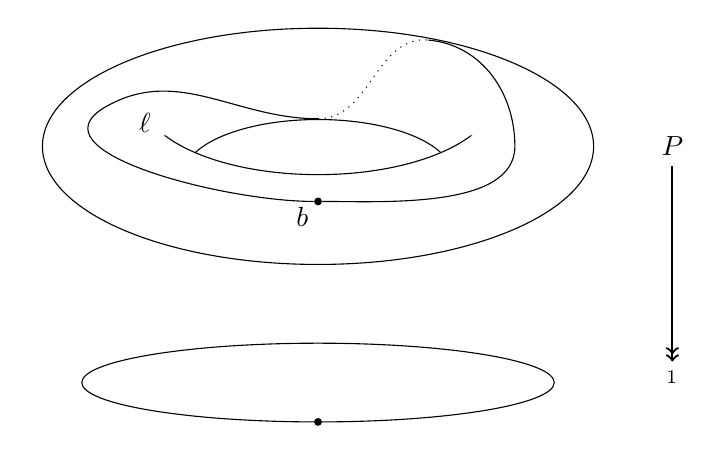
\begin{tikzpicture}
    \draw (0,0) ellipse (3 and .5);
    \draw (0,3) ellipse (3.5 and 1.5);
    \begin{scope}[yshift=4]
      \clip (-3,3) -- (-1.8,3) -- (-1.8,3.7) -- (1.8,3.7) -- (1.8,3) -- (3,3) -- (3,0) -- (-3,0) -- cycle;
      \draw[clip] (0,3.5) ellipse (2.25 and 1);
      \draw (0,2.5) ellipse (1.7 and .7);
    \end{scope}
    \node (P) at (4.5,3) {$P$};
    \node (S1) at (4.5,0) {$\Sn^1$};
    \draw[->>,thick] (P) -- (S1);
    \node[fill,circle,inner sep=1pt,label={below right:$\base$}] at (0,-.5) {};
    \node at (-2.6,.6) {$\lloop$};
    \node[fill,circle,\OPTblue,inner sep=1pt] (b) at (0,2.3) {};
    \node[\OPTblue] at (-.2,2.1) {$b$};
      \begin{scope}
        \draw[\OPTblue] (b) to[out=180,in=-150] (-2.7,3.5) to[out=30,in=180] (0,3.35);
        \draw[\OPTblue,dotted] (0,3.35) to[out=0,in=175] (1.4,4.35);
        \draw[\OPTblue] (1.4,4.35) to[out=-5,in=90] (2.5,3) to[out=-90,in=0,looseness=.8] (b);
      \end{scope}
      \node[\OPTblue] at (-2.2, 3.3) {$\ell$};
  \end{tikzpicture}
  \caption{$\Sn^1$ 的拓扑归纳原理}
  \label{fig:topS1ind}
\end{figure}

\begin{figure}
  \centering
  \begin{tikzpicture}
    \draw (0,0) ellipse (3 and .5);
    \draw (0,3) ellipse (3.5 and 1.5);
    \begin{scope}[yshift=4]
      \clip (-3,3) -- (-1.8,3) -- (-1.8,3.7) -- (1.8,3.7) -- (1.8,3) -- (3,3) -- (3,0) -- (-3,0) -- cycle;
      \draw[clip] (0,3.5) ellipse (2.25 and 1);
      \draw (0,2.5) ellipse (1.7 and .7);
    \end{scope}
    \node (P) at (4.5,3) {$P$};
    \node (S1) at (4.5,0) {$\Sn^1$};
    \draw[->>,thick] (P) -- (S1);
    \node[fill,circle,inner sep=1pt,label={below right:$\base$}] at (0,-.5) {};
    \node at (-2.6,.6) {$\lloop$};
    \node[fill,circle,\OPTblue,inner sep=1pt] (b) at (0,2.3) {};
      \node[\OPTblue] at (-.3,2.3) {$b$};
      \node[fill,circle,\OPTpurple,inner sep=1pt] (tb) at (0,1.8) {};
      % \draw[\OPTpurple,dashed] (b) to[out=0,in=0,looseness=5] (0,4) to[out=180,in=180] (tb);
      \draw[\OPTpurple,dashed] (b) arc (-90:90:2.9 and 0.85) arc (90:270:2.8 and 1.1);
      \begin{scope}
        \clip (b) -- ++(.1,0) -- (.1,1.8) -- ++(-.2,0) -- ++(0,-1) -- ++(3,2) -- ++(-3,0) -- (-.1,2.3) -- cycle;
        \draw[\OPTred,dotted,thick] (.2,2.07) ellipse (.2 and .57);
        \begin{scope}
          % \draw[clip] (b) -- ++(.1,0) |- (tb) -- ++(-.2,0) -- ++(0,-1) -| ++(3,3) -| (b);
          \clip (.2,0) rectangle (-2,3);
          \draw[\OPTred,thick] (.2,2.07) ellipse (.2 and .57);
        \end{scope}
      \end{scope}
      \node[\OPTred] at (1,1.2) {$\ell: \trans \lloop b=b$};
  \end{tikzpicture}
  \caption{$\Sn^1$ 的类型论归纳原理}
  \label{fig:ttS1ind}
\end{figure}

当然,我们期望能够从归纳原理证明递归原理,通过取 $P$ 为常值类型族。
这确实是如此,尽管从依赖计算规则(涉及 $\apdfunc f$)导出 $\lloop$ 的非依赖计算规则(涉及 $\apfunc f$)出乎意料地有些棘手。

\begin{lem}\label{thm:S1rec}
  \index{recursion principle!for S1@for $\Sn^1$}%
  \index{computation rule!for S1@for $\Sn^1$}%
  如果 $A$ 是一个类型,配备 $a:A$ 和 $p:\id[A]aa$,则存在一个函数 $f:\Sn^1\to{}A$ 满足
  \begin{align*}
    f(\base)&\defeq a \\
    \apfunc f(\lloop)&\defid p.
  \end{align*}
\end{lem}
\begin{proof}
  我们想将 $\Sn^1$ 的归纳原理应用于常值类型族 $(\lam{x} A): \Sn^1\to \UU$。
  为此所需的假设是 $(\lam{x} A)(\base) \jdeq A$ 的一个点,我们有(即 $a:A$),以及 $\dpath {x \mapsto A}{\lloop} a a$ 中的一条依赖道路,或等价地 $\transfib{x \mapsto A}{\lloop} a = a$。
  后一个类型与 $p$ 所在的类型 $\id[A]aa$ 不同,但它与之等价,因为由\cref{thm:trans-trivial}我们有 $\transconst{A}{\lloop}{a} : \transfib{x \mapsto A}{\lloop} a= a$。
  因此,给定 $a:A$ 和 $p:a=a$,我们可以考虑复合
  \[\transconst{A}{\lloop}{a} \ct p:(\dpath {x \mapsto A}\lloop aa).\]
  应用归纳原理,我们得到 $f:\Sn^1\to A$ 使得
  \begin{align}
    f(\base) &\jdeq a \qquad\text{以及}\label{eq:S1recindbase}\\
    \apdfunc f(\lloop) &= \transconst{A}{\lloop}{a} \ct p.\label{eq:S1recindloop}
  \end{align}
  还需要导出等式 $\apfunc f(\lloop)=p$。
  然而,由\cref{thm:apd-const},我们有
  \[\apdfunc f(\lloop) = \transconst{A}{\lloop}{f(\base)} \ct \apfunc f(\lloop).\]
  将此与\eqref{eq:S1recindloop}结合并消去 $\transconstf$ 的出现(由\eqref{eq:S1recindbase}它们是相同的),我们得到 $\apfunc f(\lloop)=p$。
\end{proof}

% Similarly, in this case we speak of defining $f$ by $f(\base)\defeq a$ and $\ap f \lloop \defid p$.
我们还有一个相应的唯一性原理。

\begin{lem}\label{thm:uniqueness-for-functions-on-S1}
  \index{uniqueness!principle, propositional!for functions on the circle}%
  如果 $A$ 是一个类型且 $f,g:\Sn^1\to{}A$ 是两个映射,配备两个等式 $p,q$:
  \begin{align*}
    p:f(\base)&=_Ag(\base),\\
    q:\map{f}\lloop&=^{\lam{x} x=_Ax}_p\map{g}\lloop.
  \end{align*}
  则对所有 $x:\Sn^1$ 我们有 $f(x)=g(x)$。
\end{lem}
\begin{proof}
  我们将 $\Sn^1$ 的归纳原理应用于类型族 $P(x)\defeq(f(x)=g(x))$。
  当 $x$ 是 $\base$ 时,$p$ 正是我们所需的。
  当 $x$ 沿 $\lloop$ 变化时,我们需要
  \(p=^{\lam{x} f(x)=g(x)}_{\lloop} p,\)
  这由\cref{thm:transport-path,thm:dpath-path}可归约为 $q$。
\end{proof}

\index{universal!property!of S1@of $\Sn^1$}%
这两个引理蕴含圆周的期望泛性质:

\begin{lem}\label{thm:S1ump}
  对任意类型 $A$,我们有一个自然等价
  \[ (\Sn^1 \to A) \;\eqvsym\;
  \sm{x:A} (x=x).
  \]
\end{lem}
\begin{proof}
  我们有一个由 $f(g) \defeq (g(\base),\ap g \lloop)$ 定义的典范函数 $f:(\Sn^1 \to A) \to \sm{x:A} (x=x)$。
  反方向,我们有 $g:\sm{x:A} (x=x) \to (\Sn^1 \to A)$,它将一对 $(b,\ell)$ 映射到由圆周的递归原理给出的函数 $\Sn^1 \to A$。

  现在,由递归原理的计算规则,$f \circ g \htpy \idfunc$。
  而 $g \circ f \htpy \idfunc$ 由唯一性原理得出,
  因为 \((g \circ f)(\lloop) =^{\lam{x} x=_Ax}_{\refl{\base}} \lloop\),再次由圆周的递归原理的计算规则。
  因此,$f$ 有一个拟逆,从而是一个等价。
\end{proof}

\index{type!circle|)}%

如\cref{sec:htpy-inductive}中那样,我们可以证明\cref{thm:S1ump}的结论等价于具有带命题计算规则的归纳原理。
其他高阶归纳类型也满足类似于\cref{thm:S1rec,thm:S1ump}的引理;我们通常将其证明留给读者。
我们现在继续考虑许多例子。


\section{区间}
\label{sec:interval}

\index{type!interval|(defstyle}%
\indexsee{interval!type}{type, interval}%
\define{区间},我们记作 $\interval$,可能是比圆周更简单的高阶归纳类型。
它由以下构造子生成:
\begin{itemize}
\item 一个点 $\izero:\interval$,
\item 一个点 $\ione:\interval$,以及
\item 一条道路 $\seg : \id[\interval]\izero\ione$。
\end{itemize}
\index{recursion principle!for interval type}%
区间的递归原理说如果给定类型 $B$ 连同
\begin{itemize}
\item 一个点 $b_0:B$,
\item 一个点 $b_1:B$,以及
\item 一条道路 $s:b_0=b_1$,
\end{itemize}
则存在函数 $f:\interval\to B$ 使得 $f(\izero)\jdeq b_0$,$f(\ione)\jdeq b_1$,且 $\ap f \seg = s$。
\index{induction principle!for interval type}%
归纳原理说如果给定 $P:\interval\to\type$ 连同
\begin{itemize}
\item 一个点 $b_0:P(\izero)$,
\item 一个点 $b_1:P(\ione)$,以及
\item 一条道路 $s:\dpath{P}{\seg}{b_0}{b_1}$,
\end{itemize}
则存在函数 $f:\prd{x:\interval} P(x)$ 使得 $f(\izero)\jdeq b_0$,$f(\ione)\jdeq b_1$,且 $\apd f \seg = s$。

纯粹从同伦的角度看,区间并不是很有趣:

\begin{lem}\label{thm:contr-interval}
  类型 $\interval$ 是可缩的。
\end{lem}

\begin{proof}
  我们证明对所有 $x:\interval$ 有 $x=_\interval\ione$。换言之,我们想要一个类型为 $\prd{x:\interval}(x=_\interval\ione)$ 的函数 $f$。我们以如下方式开始定义 $f$:
  \begin{alignat*}{2}
    f(\izero)&\defeq \seg  &:\izero&=_\interval\ione,\\
    f(\ione)&\defeq \refl\ione &:\ione &=_\interval\ione.
  \end{alignat*}
  还需要定义 $\apd{f}\seg$,它必须具有类型 $\seg =_\seg^{\lam{x} x=_\interval\ione}\refl \ione$。
  根据定义,这个类型是 $\trans\seg\seg=_{\ione=_\interval\ione}\refl\ione$,这又等价于 $\rev\seg\ct\seg=\refl\ione$。
  但该类型有一个典范元素,即道路逆确实是逆的证明。
\end{proof}

然而,类型论上区间确实有一些有趣的特征,就像经典同伦论中的拓扑区间一样。
例如,它使我们能够给出函数外延性的一个简单证明。
(当然,如\cref{sec:univalence-implies-funext}中那样,在以下证明期间,我们暂停我们对函数外延性公理的总体假设。)

\begin{lem}\label{thm:interval-funext}
  \index{function extensionality!proof from interval type}%
  如果 $f,g:A\to{}B$ 是两个函数使得对每个 $x:A$ 有 $f(x)=g(x)$,则在类型 $A\to{}B$ 中 $f=g$。
\end{lem}

\begin{proof}
  设我们有的证明为 $p:\prd{x:A}(f(x)=g(x))$。对所有 $x:A$ 我们定义一个函数 $\widetilde{p}_x:\interval\to{}B$,由
  \begin{align*}
    \widetilde{p}_x(\izero) &\defeq f(x), \\
    \widetilde{p}_x(\ione) &\defeq g(x), \\
    \map{\widetilde{p}_x}\seg &\defid p(x).
  \end{align*}
  我们现在定义 $q:\interval\to(A\to{}B)$,由
  \[q(i)\defeq(\lam{x} \widetilde{p}_x(i))\]
  则 $q(\izero)$ 是函数 $\lam{x} \widetilde{p}_x(\izero)$,它等于 $f$,因为 $\widetilde{p}_x(\izero)$ 由 $f(x)$ 定义。
  类似地,我们有 $q(\ione)=g$,因此
  \[\map{q}\seg:f=_{(A\to{}B)}g \qedhere\]
\end{proof}

在\cref{ex:funext-from-interval}中,我们请读者完成从\cref{thm:interval-funext}得到完整函数外延性公理的证明。

\index{type!interval|)}%

\section{圆周与球面}
\label{sec:circle}

\index{type!circle|(}%
我们已经讨论了圆周 $\Sn^1$ 作为由以下构造子生成的高阶归纳类型:
\begin{itemize}
\item 一个点 $\base:\Sn^1$,以及
\item 一条道路 $\lloop : {\id[\Sn^1]\base\base}$。
\end{itemize}
\index{induction principle!for S1@for $\Sn^1$}%
它的归纳原理说给定 $P:\Sn^1\to\type$ 连同 $b:P(\base)$ 和 $\ell :\dpath P \lloop b b$,我们有 $f:\prd{x:\Sn^1} P(x)$ 满足 $f(\base)\jdeq b$ 且 $\apd f \lloop = \ell$。
它的非依赖递归原理说给定 $B$ 配备 $b:B$ 和 $\ell:b=b$,我们有 $f:\Sn^1\to B$ 满足 $f(\base)\jdeq b$ 且 $\ap f \lloop = \ell$。

我们观察到圆周是非平凡的。

\begin{lem}\label{thm:loop-nontrivial}
  $\lloop\neq\refl{\base}$。
\end{lem}
\begin{proof}
  假设 $\lloop=\refl{\base}$。
  则由于对任意类型 $A$ 配备 $x:A$ 和 $p:x=x$,存在由 $f(\base)\defeq x$ 和 $\ap f \lloop \defid p$ 定义的函数 $f:\Sn^1\to A$,我们有
  \[p = f(\lloop) = f(\refl{\base}) = \refl{x}.\]
  但这蕴含每个类型都是集合,而我们已经看到这不是情况(见\cref{thm:type-is-not-a-set})。
\end{proof}

圆周还有以下有趣的性质,它可用作反例的来源。

\begin{lem}\label{thm:S1-autohtpy}
  存在 $\prd{x:\Sn^1} (x=x)$ 的一个元素,它不等于 $x\mapsto \refl{x}$。
\end{lem}
\begin{proof}
  我们通过 $\Sn^1$-归纳定义 $f:\prd{x:\Sn^1} (x=x)$。
  当 $x$ 是 $\base$ 时,我们令 $f(\base)\defeq \lloop$。
  现在当 $x$ 沿 $\lloop$ 变化时(见\cref{rmk:varies-along}),我们必须证明 $\transfib{x\mapsto x=x}{\lloop}{\lloop} = \lloop$。
  然而,在\cref{sec:compute-paths}中我们观察到 $\transfib{x\mapsto x=x}{p}{q} = \opp{p} \ct q \ct p$,所以我们要证明的是 $\opp{\lloop} \ct \lloop \ct \lloop = \lloop$。
  但这通过消去逆显然成立。

  要证明 $f\neq (x\mapsto \refl{x})$,只需证明 $f(\base) \neq \refl{\base}$。
  但 $f(\base)=\lloop$,所以这就是前一个引理。
\end{proof}

例如,这使我们能够扩展\cref{thm:type-is-not-a-set},证明任何包含圆周的宇宙都不能是 1-类型。

\begin{cor}
  如果类型 $\Sn^1$ 属于某个宇宙 \type,则 \type 不是 1-类型。
\end{cor}
\begin{proof}
  由泛等性,\type 中的类型 $\Sn^1=\Sn^1$ 等价于 $\Sn^1$ 的自等价类型 $\eqv{\Sn^1}{\Sn^1}$,所以只需证明 $\eqv{\Sn^1}{\Sn^1}$ 不是集合。
  \index{automorphism!of S1@of $\Sn^1$}%
  为此,只需证明其等式类型 $\id[(\eqv{\Sn^1}{\Sn^1})]{\idfunc[\Sn^1]}{\idfunc[\Sn^1]}$ 不是纯命题。
  由于是等价是纯命题,这个类型等价于 $\id[(\Sn^1\to\Sn^1)]{\idfunc[\Sn^1]}{\idfunc[\Sn^1]}$。
  但由函数外延性,这等价于 $\prd{x:\Sn^1} (x=x)$,我们在\cref{thm:S1-autohtpy}中已经看到它包含两个不相等的元素。
\end{proof}

\index{type!circle|)}%

\index{type!2-sphere|(}%
\indexsee{sphere type}{type, sphere}%
我们也提到过 2-球面 $\Sn^2$ 应该是由以下构造子生成的高阶归纳类型
\symlabel{s2b}
\begin{itemize}
\item 一个点 $\base:\Sn^2$,以及
\item 一条 2 维道路 $\surf:\refl{\base} = \refl{\base}$ 在 ${\base=\base}$ 中。
\end{itemize}
\index{recursion principle!for S2@for $\Sn^2$}%
$\Sn^2$ 的递归原理不难:它说给定 $B$ 配备 $b:B$ 和 $s:\refl b = \refl b$,我们有 $f:\Sn^2\to B$ 满足 $f(\base)\jdeq b$ 且 $\aptwo f \surf = s$。
这里``$\aptwo f \surf$''表示 $f$ 的函子作用到 2 维道路的扩展,可以精确地陈述如下。

\begin{lem}\label{thm:ap2}
  给定 $f:A\to B$ 和 $x,y:A$ 和 $p,q:x=y$,以及 $r:p=q$,我们有道路 $\aptwo f r : \ap f p = \ap f q$。
\end{lem}
\begin{proof}
  通过道路归纳,我们可以假设 $p\jdeq q$ 且 $r$ 是自反性。
  但这时我们可以定义 $\aptwo f {\refl p} \defeq \refl{\ap f p}$。
\end{proof}

为了陈述一般归纳原理,我们需要这个引理对依赖函数的一个版本,这又需要依赖 2 维道路的概念。
像以前一样,有许多方式来定义这样的东西;一种是通过传输的 2 维版本。

\begin{lem}\label{thm:transport2}
  给定 $P:A\to\type$ 和 $x,y:A$ 和 $p,q:x=y$ 和 $r:p=q$,对任意 $u:P(x)$ 我们有 $\transtwo r u : \trans p u = \trans q u$。
\end{lem}
\begin{proof}
  通过道路归纳。
\end{proof}

现在假设给定 $x,y:A$ 和 $p,q:x=y$ 和 $r:p=q$,以及点 $u:P(x)$ 和 $v:P(y)$ 和依赖道路 $h:\dpath P p u v$ 和 $k:\dpath P q u v$。
由我们对依赖道路的定义,这意味着 $h:\trans p u = v$ 且 $k:\trans q u = v$。
因此,将位于 $r$ 上方的依赖 2-道路的类型定义为
\[ (\dpath P r h k )\defeq (h = \transtwo r u \ct k) \]
是合理的。
我们现在可以陈述\cref{thm:ap2}的依赖版本。

\begin{lem}\label{thm:apd2}
  给定 $P:A\to\type$ 和 $x,y:A$ 和 $p,q:x=y$ 和 $r:p=q$ 以及函数 $f:\prd{x:A} P(x)$,我们有
  $\apdtwo f r : \dpath P r {\apd f p}{\apd f q}$。
\end{lem}
\begin{proof}
  道路归纳。
\end{proof}

\index{induction principle!for S2@for $\Sn^2$}%
现在我们可以陈述 $\Sn^2$ 的归纳原理:假设给定 $P:\Sn^2\to\type$ 配备 $b:P(\base)$ 和 $s:\dpath Q \surf {\refl b}{\refl b}$,其中 $Q\defeq\lam{p} \dpath P p b b$。则存在函数 $f:\prd{x:\Sn^2} P(x)$ 使得 $f(\base)\jdeq b$ 且 $\apdtwo f \surf = s$。

\index{type!2-sphere|)}%

当然,随着维度的增加,这种显式方法变得越来越复杂。
因此,如果我们想为所有 $n$ 定义 $n$-球面,我们需要一些更系统的想法。
一种方法是直接使用 $n$ 维环路\index{loop!n-@$n$-},而不是一般的 $n$ 维道路\index{path!n-@$n$-}。

\index{type!pointed}%
回顾\cref{sec:equality}中\emph{点型类型} $\type_*$ 和 $n$ 重环路空间\index{loop space!iterated} $\Omega^n : \type_* \to \type_*$ 的定义
(\cref{def:pointedtype,def:loopspace})。现在我们可以将 $n$-球面 $\Sn^n$ 定义为由以下构造子生成的高阶归纳类型
\index{type!n-sphere@$n$-sphere}%
\begin{itemize}
\item 一个点 $\base:\Sn^n$,以及
\item 一个 $n$-环路 $\lloop_n : \Omega^n(\Sn^n,\base)$。
\end{itemize}
为了写出这种表示的归纳原理,我们需要定义``依赖 $n$-环路\indexdef{loop!dependent n-@dependent $n$-}''的概念,以及依赖函数在 $n$-环路上的作用。
我们将此留给读者(见\cref{ex:nspheres});在下一节中,我们将讨论另一种有时更易处理的球面定义方式。


\section{悬挂}
\label{sec:suspension}

\indexsee{type!suspension of}{suspension}%
\index{suspension|(defstyle}%
类型 $A$ 的\define{悬挂}是将 $A$ 的点变成道路的泛方式(从而 $A$ 中的道路变成 2-道路,等等)。
它是由以下生成元定义的类型 $\susp A$:\footnote{与依赖对类型有一个不幸的记号冲突,当然后者也用 $\Sigma$ 书写。然而,上下文通常能消歧义。}
\begin{itemize}
\item 一个点 $\north:\susp A$,
\item 一个点 $\south:\susp A$,以及
\item 一个函数 $\merid:A \to (\id[\susp A]\north\south)$。
\end{itemize}
这些名称意在暗示某种``球体'',有北极、南极,以及 $A$ 那么多的经线
\indexdef{pole}%
\indexdef{meridian}%
从一个到另一个。
事实上,正如我们将看到的,如果 $A=\Sn^1$,则其悬挂等价于普通球面的表面 $\Sn^2$。

\index{recursion principle!for suspension}%
$\susp A$ 的递归原理说给定类型 $B$ 连同
\begin{itemize}
\item 点 $n,s:B$,以及
\item 函数 $m:A \to (n=s)$,
\end{itemize}
我们有函数 $f:\susp A \to B$ 使得 $f(\north)\jdeq n$ 且 $f(\south)\jdeq s$,并且对所有 $a:A$ 我们有 $\ap f {\merid(a)} = m(a)$。
\index{induction principle!for suspension}%
类似地,归纳原理说给定 $P:\susp A \to \type$ 连同
\begin{itemize}
\item 一个点 $n:P(\north)$,
\item 一个点 $s:P(\south)$,以及
\item 对每个 $a:A$,一条道路 $m(a):\dpath P{\merid(a)}ns$,
\end{itemize}
存在函数 $f:\prd{x:\susp A} P(x)$ 使得 $f(\north)\jdeq n$ 且 $f(\south)\jdeq s$,并且对每个 $a:A$ 我们有 $\apd f {\merid(a)} = m(a)$。

我们关于悬挂的第一个观察是它提供了定义圆周的另一种方式。

\begin{lem}\label{thm:suspbool}
  \index{type!circle}%
  $\eqv{\susp\bool}{\Sn^1}$。
\end{lem}
\begin{proof}
  通过递归定义 $f:\susp\bool\to\Sn^1$,使得 $f(\north)\defeq \base$ 且 $f(\south)\defeq\base$,同时 $\ap f{\merid(\bfalse)}\defid\lloop$ 但 $\ap f{\merid(\btrue)} \defid \refl{\base}$。
  通过递归定义 $g:\Sn^1\to\susp\bool$,使得 $g(\base)\defeq \north$ 且 $\ap g \lloop \defid \merid(\bfalse) \ct \opp{\merid(\btrue)}$。
  我们现在证明 $f$ 和 $g$ 是拟逆。

  首先通过归纳证明对所有 $x:\susp \bool$ 有 $g(f(x))=x$。
  如果 $x\jdeq\north$,则 $g(f(\north)) \jdeq g(\base)\jdeq \north$,所以我们有 $\refl{\north} : g(f(\north))=\north$。
  如果 $x\jdeq\south$,则 $g(f(\south)) \jdeq g(\base)\jdeq \north$,我们选择等式 $\merid(\btrue) : g(f(\south)) = \south$。
  还需证明对任意 $y:\bool$,这些等式在 $x$ 沿 $\merid(y)$ 变化时保持,即当 $\refl{\north}$ 沿 $\merid(y)$ 传输时得到 $\merid(\btrue)$。
  由道路空间和拉回纤维化中的传输,这意味着我们要证明
  \[ \opp{\ap g {\ap f {\merid(y)}}} \ct \refl{\north} \ct \merid(y) = \merid(\btrue). \]
  当然,我们可以消去 $\refl{\north}$。
  现在通过 \bool-归纳,我们可以假设 $y\jdeq \bfalse$ 或 $y\jdeq \btrue$。
  如果 $y\jdeq \bfalse$,则我们有
  \begin{align*}
    \opp{\ap g {\ap f {\merid(\bfalse)}}} \ct \merid(\bfalse)
    &= \opp{\ap g {\lloop}} \ct \merid(\bfalse)\\
    &= \opp{(\merid(\bfalse) \ct \opp{\merid(\btrue)})} \ct \merid(\bfalse)\\
    &= \merid(\btrue) \ct \opp{\merid(\bfalse)} \ct \merid(\bfalse)\\
    &= \merid(\btrue)
  \end{align*}
  而如果 $y\jdeq \btrue$,则我们有
  \begin{align*}
    \opp{\ap g {\ap f {\merid(\btrue)}}} \ct \merid(\btrue)
    &= \opp{\ap g {\refl{\base}}} \ct \merid(\btrue)\\
    &= \opp{\refl{\north}} \ct \merid(\btrue)\\
    &= \merid(\btrue).
  \end{align*}
  因此,对所有 $x:\susp \bool$,我们有 $g(f(x))=x$。

  现在通过归纳证明对所有 $x:\Sn^1$ 有 $f(g(x))=x$。
  如果 $x\jdeq \base$,则 $f(g(\base))\jdeq f(\north)\jdeq\base$,所以我们有 $\refl{\base} : f(g(\base))=\base$。
  还需证明这个等式在 $x$ 沿 $\lloop$ 变化时保持,即它沿 $\lloop$ 传输到自身。
  再次,由道路空间和拉回纤维化中的传输,这意味着要证明
  \[ \opp{\ap f {\ap g {\lloop}}} \ct \refl{\base} \ct \lloop = \refl{\base}.\]
  然而,我们有
  \begin{align*}
    \ap f {\ap g {\lloop}} &= \ap f {\merid(\bfalse) \ct \opp{\merid(\btrue)}}\\
    &= \ap f {\merid(\bfalse)} \ct \opp{\ap f {\merid(\btrue)}}\\
    &= \lloop \ct \refl{\base}
  \end{align*}
  所以这容易得出。
\end{proof}

拓扑上,两点空间 \bool 也被称为\emph{0 维球面} $\Sn^0$。
(例如,它是 $\mathbb{R}^1$ 中到原点距离为 $1$ 的点的空间,就像拓扑 1-球面是 $\mathbb{R}^2$ 中到原点距离为 $1$ 的点的空间一样。)
因此,\cref{thm:suspbool}可以暗示性地表述为 $\eqv{\susp\Sn^0}{\Sn^1}$。
\index{type!n-sphere@$n$-sphere|defstyle}%
\indexsee{n-sphere@$n$-sphere}{type, $n$-sphere}%
事实上,这种模式继续下去:我们可以归纳地定义所有球面
\begin{equation}\label{eq:Snsusp}
  \Sn^0 \defeq \bool
  \qquad\text{且}\qquad
  \Sn^{n+1} \defeq \susp \Sn^n.
\end{equation}
我们甚至可以从低一维开始,定义 $\Sn^{-1}\defeq \emptyt$,并观察 $\eqv{\susp\emptyt}{\bool}$。

要仔细证明这与前一节中 $\Sn^n$ 的定义一致需要使后者更加明确。
然而,我们可以证明递归定义具有我们期望另一个定义具有的相同泛性质。
如果 $(A,a_0)$ 和 $(B,b_0)$ 是点型类型(基点通常省略),令 $\Map_*(A,B)$ 表示基点保持映射的类型:
\index{based map}
\symlabel{based-maps}
\[ \Map_*(A,B) \defeq \sm{f:A\to B} (f(a_0)=b_0). \]
注意任何类型 $A$ 都产生一个点型类型 $A_+ \defeq A+\unit$,其基点为 $\inr(\ttt)$;这称为\emph{添加一个不相交基点}。
\indexdef{basepoint!adjoining a disjoint}%
\index{disjoint!basepoint}%
\index{adjoining a disjoint basepoint}%

\begin{lem}
  对于类型 $A$ 和点型类型 $(B,b_0)$,我们有
  \[ \eqv{\Map_*(A_+,B)}{(A\to B)} \]
\end{lem}
注意右边是从 $A$ 到 $B$ 的\emph{非基点保持}函数的普通类型。
\begin{proof}
  从左到右,给定 $f:A_+ \to B$ 配备 $p:f(\inr(\ttt)) = b_0$,我们有 $f\circ \inl : A \to B$。
  从右到左,给定 $g:A\to B$ 我们定义 $g':A_+ \to B$,由 $g'(\inl(a))\defeq g(a)$ 且 $g'(\inr(u)) \defeq b_0$。
  我们将证明这些是拟逆运算留给读者。
\end{proof}

特别地,注意 $\eqv{\bool}{\unit_+}$。
因此,对任意点型类型 $B$ 我们有
\[{\Map_*(\bool,B)} \eqvsym {(\unit \to B)}\eqvsym B.\]
%
现在回顾环路空间\index{loop space}运算 $\Omega$ 作用于点型类型,定义为 $\Omega(A,a_0) \defeq (\id[A]{a_0}{a_0},\refl{a_0})$。
我们也可以使悬挂 $\susp$ 作用于点型类型,由 $\susp(A,a_0)\defeq (\susp A,\north)$。

\begin{lem}\label{lem:susp-loop-adj}
  \index{universal!property!of suspension}%
  对于点型类型 $(A,a_0)$ 和 $(B,b_0)$,我们有
  \[ \eqv{\Map_*(\susp A, B)}{\Map_*(A,\Omega B)}.\]
\end{lem}
\addtocounter{thm}{1}           % Because we removed a numbered equation in commit 8f54d16
\begin{proof}
我们首先观察以下等价链:
\begin{align*}
\Map_*(\susp A, B) & \defeq \sm{f:\susp A\to B} (f(\north)=b_0) \\
                   & \eqvsym \sm{f:\sm{b_n : B}{b_s : B} (A \to (b_n = b_s))} (\fst(f)=b_0) \\
                   & \eqvsym \sm{b_n : B}{b_s : B} \big(A \to (b_n = b_s)\big) \times (b_n=b_0) \\
                   & \eqvsym \sm{p : \sm{b_n : B} (b_n=b_0)}{b_s : B} (A \to (\fst(p) = b_s)) \\
                   & \eqvsym \sm{b_s : B} (A \to (b_0 = b_s))
\end{align*}
第一个等价由悬挂的泛性质得出,即
\[ \Parens{\susp A \to B} \eqvsym \Parens{\sm{b_n : B} \sm{b_s : B} (A \to (b_n = b_s)) } \]
其中从右到左的函数由递归器给出(见\cref{ex:susp-lump})。
第二个和第三个等价由\cref{ex:sigma-assoc}得出,连同分量的重排。
最后,最后一个等价由\cref{thm:omit-contr}得出,因为由\cref{thm:contr-paths},$\sm{b_n : B} (b_n=b_0)$ 是以 $(b_0, \refl{b_0})$ 为中心的可缩类型。

证明现在由以下等价链完成:
\begin{align*}
  \sm{b_s : B} (A \to (b_0 = b_s))
  &\eqvsym \sm{b_s : B}{g:A \to (b_0 = b_s)}{q:b_0 = b_s} (g(a_0) = q)\\
  &\eqvsym \sm{r : \sm{b_s : B}(b_0 = b_s)}{g:A \to (b_0 = \proj1(r))} (g(a_0) = \proj2(r))\\
  &\eqvsym \sm{g:A \to (b_0 = b_0)} (g(a_0) = \refl{b_0})\\
  &\jdeq \Map_*(A,\Omega B).
\end{align*}
与之前类似,第一个和最后一个等价由\cref{thm:omit-contr,thm:contr-paths}得出,第二个由\cref{ex:sigma-assoc}和分量的重排得出。
\end{proof}

\index{type!n-sphere@$n$-sphere|defstyle}%
特别地,对于按\eqref{eq:Snsusp}定义的球面,我们有
\index{universal!property!of Sn@of $\Sn^n$}%
\[ \Map_*(\Sn^n,B) \eqvsym \Map_*(\Sn^{n-1}, \Omega B) \eqvsym \cdots \eqvsym \Map_*(\bool,\Omega^n B) \eqvsym \Omega^n B. \]
因此,这些球面 $\Sn^n$ 具有我们从\cref{sec:circle}中直接用 $n$ 重环路空间\index{loop space!iterated}定义的球面所期望的泛性质。

\index{suspension|)}%

\section{胞腔复形}
\label{sec:cell-complexes}

\index{cell complex|(defstyle}%
\index{CW complex|(defstyle}%
在经典拓扑中,\emph{胞腔复形}是通过沿边界依次粘贴圆盘获得的空间。
如果 $n$ 维圆盘\index{disc}的边界被约束在维数严格小于 $n$ 的圆盘中($(n-1)$-骨架),则称为\emph{CW 复形}\index{skeleton!of a CW-complex}。

任何有限 CW 复形都可以表示为高阶归纳类型,方法是将 $n$ 维圆盘变成 $n$ 维道路,并将粘贴映射\index{attaching map}的像分成源\index{source!of a path constructor}和靶\index{target!of a path constructor},每个都写成低维道路的复合。
我们在\cref{sec:circle}中对 $\Sn^1$ 和 $\Sn^2$ 的显式定义就是这种形式。

\index{torus}%
另一个例子是环面 $T^2$,它由以下构造子生成:
\begin{itemize}
\item 一个点 $b:T^2$,
\item 一条道路 $p:b=b$,
\item 另一条道路 $q:b=b$,以及
\item 一条 2-道路 $t: p\ct q = q \ct p$。
\end{itemize}
也许看出这是环面的最简单方式是从一个矩形开始,有四个角 $a,b,c,d$,四条边 $p,q,r,s$,和一个内部,它显然是从 $p\ct q$ 到 $r\ct s$ 的 2-道路 $t$:
\begin{equation*}
  \xymatrix{
      a\ar@{=}[r]^p\ar@{=}[d]_r \ar@{}[dr]|{\Downarrow t} &
      b\ar@{=}[d]^q\\
      c\ar@{=}[r]_s &
      d
      }
\end{equation*}
现在将边 $r$ 与 $q$ 等同,边 $s$ 与 $p$ 等同,结果也将所有四个角等同。
拓扑上,这种等同可以被看作产生一个环面。

\index{induction principle!for torus}%
\index{torus!induction principle for}%
环面的归纳原理是我们目前写出的最棘手的。
给定 $P:T^2\to\type$,对于一个截面 $\prd{x:T^2} P(x)$,我们需要
\begin{itemize}
\item 一个点 $b':P(b)$,
\item 一条道路 $p' : \dpath P p {b'} {b'}$,
\item 一条道路 $q' : \dpath P q {b'} {b'}$,以及
\item 一条 2-道路 $t'$,介于``复合'' $p'\ct q'$ 和 $q'\ct p'$ 之间,位于 $t$ 上方。
\end{itemize}
为了理解最后一个数据,我们需要依赖道路的复合运算,但这不难定义。
然后归纳原理给出函数 $f:\prd{x:T^2} P(x)$ 使得 $f(b)\jdeq b'$ 且 $\apd f {p} = p'$ 且 $\apd f {q} = q'$ 以及类似``$\apdtwo f t = t'$''的东西。
然而,这作为陈述并不良型,首先因为等式 $\apd f {p} = p'$ 和 $\apd f {q} = q'$ 不是判断的,其次因为 $\apdfunc f$ 只在同伦意义下保持道路串联。
我们将细节留给读者(见\cref{ex:torus})。

当然,环面的另一个定义是 $T^2 \defeq \Sn^1 \times \Sn^1$(在\cref{ex:torus-s1-times-s1}中我们请读者验证这两者的等价性)。
\index{Klein bottle}%
\index{projective plane}%
然而,胞腔复形的定义很容易推广到没有这类描述的其他空间,如克莱因瓶、射影平面等。
但写出归纳原理确实变得越来越困难,需要我们定义依赖 $n$-道路的概念以及 $\apdfunc{}$ 作用于 $n$-道路。
幸运的是,一旦我们有了球面,就有一种方法可以绕过这个问题。

\section{轮毂与辐条}
\label{sec:hubs-spokes}

\indexsee{spoke}{hub and spoke}%
\index{hub and spoke|(defstyle}%

在拓扑中,人们通常说通过沿其 $(n-1)$ 维边界球面粘贴 $n$ 维圆盘来构建 CW 复形。
\index{attaching map}%
然而,另一种表达方式是粘入 $(n-1)$ 维球面的\emph{锥}%
\index{cone!of a sphere}。
也就是说,我们将圆盘\index{disc}视为由一个锥点(或``轮毂'')组成,连续地用经线
\index{meridian}%
(或``辐条'')将该点连接到边界上的每一点,如\cref{fig:hub-and-spokes}所示。

\begin{figure}
  \centering
  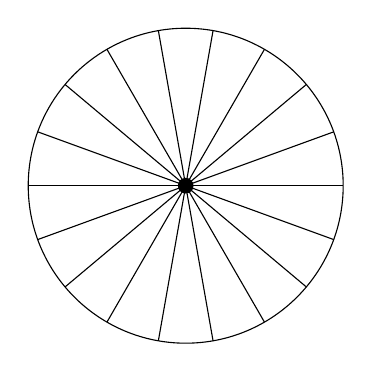
\begin{tikzpicture}
    \draw (0,0) circle (2cm);
    \foreach \x in {0,20,...,350}
      \draw[\OPTblue] (0,0) -- (\x:2cm);
    \node[\OPTblue,circle,fill,inner sep=2pt] (hub) at (0,0) {};
  \end{tikzpicture}
  \caption{由轮毂和辐条组成的 2-圆盘}
  \label{fig:hub-and-spokes}
\end{figure}

我们可以使用这个想法将包含 $n>1$ 维道路构造子的高阶归纳类型用只包含 1 维道路构造子的类型来表达。
关键是我们可以将 $n$ 维道路作为由 $(n-1)$ 维对象参数化的 1 维道路的连续族获得。
最简单的 $(n-1)$ 维对象是 $(n-1)$-球面,尽管在某些情况下可能更喜欢不同的对象。
(回想我们在\cref{sec:suspension}中能够使用悬挂归纳地定义球面,而悬挂只涉及 1 维道路构造子。
事实上,悬挂也可以看作是这个想法的一个实例,因为它涉及由被悬挂类型参数化的 1 维道路族。)

\index{torus}
例如,上一节的环面 $T^2$ 可以改为由以下构造子生成:
\begin{itemize}
\item 一个点 $b:T^2$,
\item 一条道路 $p:b=b$,
\item 另一条道路 $q:b=b$,
\item 一个点 $h:T^2$,以及
\item 对每个 $x:\Sn^1$,一条道路 $s(x) : f(x)=h$,其中 $f:\Sn^1\to T^2$ 由 $f(\base)\defeq b$ 和 $\ap f \lloop \defid p \ct q \ct \opp p \ct \opp q$ 定义。
\end{itemize}
这个版本的环面的归纳原理说给定 $P:T^2\to\type$,对于一个截面 $\prd{x:T^2} P(x)$,我们需要
\begin{itemize}
\item 一个点 $b':P(b)$,
\item 一条道路 $p' : \dpath P p {b'} {b'}$,
\item 一条道路 $q' : \dpath P q {b'} {b'}$,
\item 一个点 $h':P(h)$,以及
\item 对每个 $x:\Sn^1$,一条道路 $\dpath {P}{s(x)}{g(x)}{h'}$,其中 $g:\prd{x:\Sn^1} P(f(x))$ 由 $g(\base)\defeq b'$ 和 $\apd g \lloop \defid t(p' \ct q' \ct \opp{(p')} \ct \opp{(q')})$ 定义。
  在后者中,$\ct$ 表示依赖道路的串联,而 $t:\eqv{(\dpath{P}{\ap f \lloop}{b'}{b'})}{(\dpath{P\circ f}{\lloop}{b'}{b'})}$ 的定义留给读者。
\end{itemize}
注意不需要依赖 2-道路或 $\apdtwofunc{}$。
我们将计算规则的写出留给读者。

\begin{rmk}\label{rmk:spokes-no-hub}
人们可能会质疑引入轮毂点 $h$ 的必要性;为什么我们不能简单地添加道路,连续地将圆盘的边界关联到该边界\emph{上}的一点,如\cref{fig:spokes-no-hub}所示?
然而,这在没有进一步修改的情况下是行不通的。
因为如果给定某个 $f:\Sn^1 \to X$,我们给出一个道路构造子连接每个 $f(x)$ 到 $f(\base)$,那么我们最终得到的更像是\cref{fig:spokes-no-hub-ii}中的图片,一个锥的顶点被扭曲并粘贴到其底部的某点上。
问题是从 $f(\base)$ 到自身的指定道路可能不是自反性。
我们可以通过添加一个 2 维道路构造子来补救这个问题以确保这一点,但使用一个单独的轮毂避免了对维度高于 1 的任何道路构造子的需要。
\end{rmk}

\begin{figure}
  \centering
  \begin{minipage}{2in}
    \begin{center}
      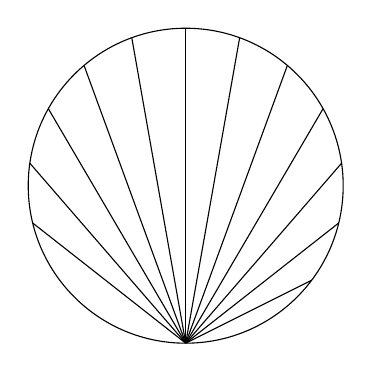
\begin{tikzpicture}
        \draw (0,0) circle (2cm);
        \clip (0,0) circle (2cm);
        \foreach \x in {0,15,...,165}
        \draw[\OPTblue] (0,-2cm) -- (\x:4cm);
      \end{tikzpicture}
    \end{center}
    \caption{无轮毂的辐条}
    \label{fig:spokes-no-hub}
  \end{minipage}
  \qquad
  \begin{minipage}{2in}
    \begin{center}
      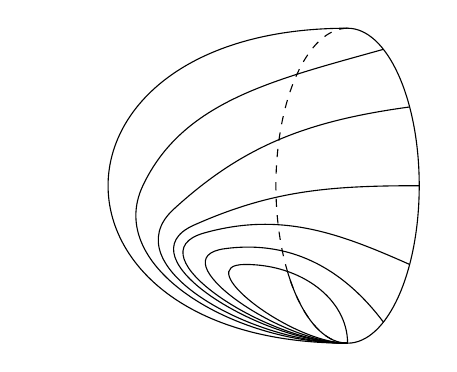
\begin{tikzpicture}[xscale=1.3]
        \draw (0,0) arc (-90:90:.7cm and 2cm) ;
        \draw[dashed] (0,4cm) arc (90:270:.7cm and 2cm) ;
        \draw[\OPTblue] (0,0) to[out=90,in=0] (-1,1) to[out=180,in=180] (0,0);
        \draw[\OPTblue] (0,4cm) to[out=180,in=180,looseness=2] (0,0);
        \path (0,0) arc (-90:-60:.7cm and 2cm) node (a) {};
        \draw[\OPTblue] (a.center) to[out=120,in=10] (-1.2,1.2) to[out=190,in=180] (0,0);
        \path (0,0) arc (-90:-30:.7cm and 2cm) node (b) {};
        \draw[\OPTblue] (b.center) to[out=150,in=20] (-1.4,1.4) to[out=200,in=180] (0,0);
        \path (0,0) arc (-90:0:.7cm and 2cm) node (c) {};
        \draw[\OPTblue] (c.center) to[out=180,in=30] (-1.5,1.5) to[out=210,in=180] (0,0);
        \path (0,0) arc (-90:30:.7cm and 2cm) node (d) {};
        \draw[\OPTblue] (d.center) to[out=190,in=50] (-1.7,1.7) to[out=230,in=180] (0,0);
        \path (0,0) arc (-90:60:.7cm and 2cm) node (e) {};
        \draw[\OPTblue] (e.center) to[out=200,in=70] (-2,2) to[out=250,in=180] (0,0);
        \clip (0,0) to[out=90,in=0] (-1,1) to[out=180,in=180] (0,0);
        \draw (0,4cm) arc (90:270:.7cm and 2cm) ;
      \end{tikzpicture}
    \end{center}
    \caption{无轮毂的辐条,II}
    \label{fig:spokes-no-hub-ii}
  \end{minipage}
\end{figure}

\begin{rmk}
  \index{computation rule!propositional}%
  还要注意,这种将高阶道路``翻译''为 1-道路的方式不保留这些道路的判断计算规则,尽管它确实保留命题计算规则。
\end{rmk}

\index{cell complex|)}%
\index{CW complex|)}%

\index{hub and spoke|)}%


\section{推出}
\label{sec:colimits}

\index{type!limit}%
\index{type!colimit}%
\index{limit!of types}%
\index{colimit!of types}%
从范畴论的角度来看,任何基础系统的重要方面之一是构造极限和余极限的能力。
在集合论基础中,这些是集合的极限和余极限,而在我们的情况下,它们是\emph{类型}的极限和余极限。
我们在\cref{sec:universal-properties}中看到笛卡尔积类型具有类型的范畴积的正确泛性质,在\cref{ex:coprod-ump}中看到余积类型同样具有其期望的泛性质。

如\cref{sec:universal-properties}中所述,更一般的极限可以使用恒等类型和 $\Sigma$-类型来构造,例如 $f:A\to C$ 和 $g:B\to C$ 的拉回\index{pullback}是 $\sm{a:A}{b:B} (f(a)=g(b))$(见\cref{ex:pullback})。
然而,更一般的\emph{余极限}需要等同来自不同类型的元素,高阶归纳类型非常适合这一点。
由于我们所有的构造都是同伦不变的,我们所有的余极限必然是\emph{同伦余极限},但为简洁起见,我们省略这个普遍的形容词。

在本节中,我们讨论\emph{推出},作为也许最简单和最有用的余极限之一。
事实上,人们期望所有有限余极限(对于``有限''的适当同伦定义)都可以从推出和有限余积构造。
也可以使用高阶归纳类型直接构造更一般的余极限,但这有些技术性,而且也不完全令人满意,因为我们还没有一个好的同伦相容图的完全一般概念。

\indexsee{type!pushout of}{pushout}%
\index{pushout|(defstyle}%
\index{span}%
假设给定类型和函数的跨越:
\[\Ddiag=\;\vcenter{\xymatrix{C \ar^g[r] \ar_f[d] & B \\ A & }}\]
这个跨越的\define{推出}是由以下呈现的高阶归纳类型 $A\sqcup^CB$:
\begin{itemize}
\item 一个函数 $\inl:A\to A\sqcup^CB$,
\item 一个函数 $\inr:B \to A\sqcup^CB$,以及
\item 对每个 $c:C$ 一条道路 $\glue(c):(\inl(f(c))=\inr(g(c)))$。
\end{itemize}
换言之,$A\sqcup^CB$ 是 $A$ 和 $B$ 的不相交并,连同对每个 $c:C$ 一个 $f(c)$ 和 $g(c)$ 相等的见证。
递归原理说如果 $D$ 是另一个类型,我们可以通过定义以下来定义映射 $s:A\sqcup^CB\to{}D$:
\begin{itemize}
\item 对每个 $a:A$,$s(\inl(a)):D$ 的值,
\item 对每个 $b:B$,$s(\inr(b)):D$ 的值,以及
\item 对每个 $c:C$,$\mapfunc{s}(\glue(c)):s(\inl(f(c)))=s(\inr(g(c)))$ 的值。
\end{itemize}
我们将归纳原理的表述留给读者。
它还蕴含唯一性原理,即如果 $s,s':A\sqcup^CB\to{}D$ 是两个映射使得
\index{uniqueness!principle, propositional!for functions on a pushout}%
\begin{align*}
  s(\inl(a))&=s'(\inl(a))\\
  s(\inr(b))&=s'(\inr(b))\\
  \mapfunc{s}(\glue(c))&=\mapfunc{s'}(\glue(c))
  \qquad\text{(模前两个等式)}
\end{align*}
对每个 $a,b,c$ 成立,则 $s=s'$。

为了表述推出的泛性质,我们引入以下定义。

\begin{defn}\label{defn:cocone}
  给定跨越 $\Ddiag= (A \xleftarrow{f} C \xrightarrow{g} B)$ 和类型 $D$,\define{顶点为 $D$ 的 $\Ddiag$ 下的余锥}
  \indexdef{cocone}%
  \index{vertex of a cocone}%
  由函数 $i:A\to{}D$ 和 $j:B\to{}D$ 以及同伦 $h : \prd{c:C} (i(f(c))=j(g(c)))$ 组成:
  \[\uppercurveobject{{ }}\lowercurveobject{{ }}\twocellhead{{ }}
  \xymatrix{C \ar^g[r] \ar_f[d] \drtwocell{^h} & B \ar^j[d] \\ A \ar_i[r] & D
  }\]
  我们用 $\cocone{\Ddiag}{D}$ 表示所有这类余锥的类型,即
  \[ \cocone{\Ddiag}{D} \defeq
  \sm{i:A\to D}{j:B\to D} \prd{c:C} (i(f(c))=j(g(c))).
  \]
\end{defn}

当然,存在顶点为 $A\sqcup^C B$ 的 $\Ddiag$ 下的一个典范余锥,由 $\inl$、$\inr$ 和 $\glue$ 组成。
\[\uppercurveobject{{ }}\lowercurveobject{{ }}\twocellhead{{ }}
\xymatrix{C \ar^g[r] \ar_f[d] \drtwocell{^\glue\ \ } & B \ar^\inr[d] \\
  A \ar_-\inl[r] & A\sqcup^CB }\]
以下引理说这是泛余锥。

\begin{lem}\label{thm:pushout-ump}
  \index{universal!property!of pushout}%
  对任意类型 $E$,存在等价
  \[ (A\sqcup^C B \to E) \;\eqvsym\; \cocone{\Ddiag}{E}. \]
\end{lem}
\begin{proof}
  考虑任意类型 $E:\type$。
  存在由以下定义的典范函数 $c_\sqcup$
  \[\function{(A\sqcup^CB\to{}E)}{\cocone{\Ddiag}{E}}
  {t}{(t\circ{}\inl,t\circ{}\inr,\mapfunc{t}\circ{}\glue)}\]
  我们非形式地将这个函数写作 $t\mapsto\composecocone{t}c_\sqcup$。
  我们证明这是一个等价。

  首先,给定 $c=(i,j,h):\cocone{\mathscr{D}}{E}$,我们需要构造一个从 $A\sqcup^CB$ 到 $E$ 的映射 $\mathsf{s}(c)$。
  \[\uppercurveobject{{ }}\lowercurveobject{{ }}\twocellhead{{ }}
  \xymatrix{C \ar^g[r] \ar_f[d] \drtwocell{^h} & B \ar^{j}[d] \\
    A \ar_-{i}[r] & E }\]
 映射 $\mathsf{s}(c)$ 以如下方式定义
  \begin{align*}
    \mathsf{s}(c)(\inl(a))&\defeq i(a),\\
    \mathsf{s}(c)(\inr(b))&\defeq j(b),\\
    \mapfunc{\mathsf{s}(c)}(\glue(x))&\defid h(x).
  \end{align*}
我们定义了映射
\[\function{\cocone{\Ddiag}{E}}{(A\sqcup^CB\to{}E)}{c}{\mathsf{s}(c)}\]
我们需要证明这个映射是 $t\mapsto{}\composecocone{t}c_\sqcup$ 的逆。
一方面,如果 $c=(i,j,h):\cocone{\Ddiag}{E}$,我们有
\begin{align*}
  \composecocone{\mathsf{s}(c)}c_\sqcup & =
  (\mathsf{s}(c)\circ\inl,\mathsf{s}(c)\circ\inr,
  \mapfunc{\mathsf{s}(c)}\circ\glue) \\
  & = (\lamu{a:A} \mathsf{s}(c)(\inl(a)),\;
  \lamu{b:B} \mathsf{s}(c)(\inr(b)),\;
  \lamu{x:C} \mapfunc{\mathsf{s}(c)}(\glue(x))) \\
  & = (\lamu{a:A} i(a),\;
  \lamu{b:B} j(b),\;
  \lamu{x:C} h(x)) \\
  & \jdeq (i, j, h) \\
  & = c.
\end{align*}
%
另一方面,如果 $t:A\sqcup^CB\to{}E$,我们想证明
$\mathsf{s}(\composecocone{t}c_\sqcup)=t$。
对 $a:A$,我们有
\[\mathsf{s}(\composecocone{t}c_\sqcup)(\inl(a))=t(\inl(a))\]
因为 $\composecocone{t}c_\sqcup$ 的第一个分量是 $t\circ\inl$。以同样的方式,对 $b:B$ 我们有
\[\mathsf{s}(\composecocone{t}c_\sqcup)(\inr(b))=t(\inr(b))\]
对 $x:C$ 我们有
\[\mapfunc{\mathsf{s}(\composecocone{t}c_\sqcup)}(\glue(x))
=\mapfunc{t}(\glue(x))\]
因此 $\mathsf{s}(\composecocone{t}c_\sqcup)=t$。

这证明了 $c\mapsto\mathsf{s}(c)$ 是 $t\mapsto{}\composecocone{t}c_\sqcup$ 的拟逆,如所需。
\end{proof}

许多标准的同伦论构造可以表示为(同伦)推出。
\begin{itemize}
\item 跨越 $\unit \leftarrow A \to \unit$ 的推出是\define{悬挂} $\susp A$(见\cref{sec:suspension})。%
  \index{suspension}
\symlabel{join}
\item $A \xleftarrow{\proj1} A\times B \xrightarrow{\proj2} B$ 的推出称为 $A$ 和 $B$ 的\define{连接},记作 $A*B$。%
  \indexdef{join!of types}
\item $\unit \leftarrow A \xrightarrow{f} B$ 的推出是 $f$ 的\define{锥}或\define{余纤维}。%
  \indexdef{cone!of a function}%
  \indexsee{mapping cone}{cone of a function}%
  \indexdef{cofiber of a function}%
\symlabel{wedge}
\item 如果 $A$ 和 $B$ 配备基点 $a_0:A$ 和 $b_0:B$,则 $A \xleftarrow{a_0} \unit \xrightarrow{b_0} B$ 的推出是\define{楔和} $A\vee B$。%
  \indexdef{wedge}
\symlabel{smash}
\item 如果 $A$ 和 $B$ 如前配备基点,定义 $f:A\vee B \to A\times B$,由 $f(\inl(a))\defeq (a,b_0)$ 和 $f(\inr(b))\defeq (a_0,b)$,以及 $\ap f \glue \defid \refl{(a_0,b_0)}$。
  则 $f$ 的锥称为\define{粉碎积} $A\wedge B$。%
  \indexdef{smash product}
\end{itemize}
我们将在\cref{cha:hlevels,cha:homotopy}中进一步讨论推出。

\begin{rmk}
  如\cref{subsec:prop-trunc}中所述,粉碎积和点型空间的楔和的记号 $\wedge$ 和 $\vee$ 也在逻辑中用于``与''和``或''。
  由于同伦类型论中的类型可以表现得像空间或像命题,因此技术上存在冲突的可能——但由于它们很少同时表现为两者,上下文通常能消歧义。
  此外,粉碎积和楔和只适用于\emph{点型}空间,而唯一的点型纯命题是 $\top\jdeq\unit$——且无论 $\wedge$ 和 $\vee$ 的哪种含义,我们都有 $\unit\wedge \unit = \unit$ 和 $\unit\vee\unit=\unit$。
\end{rmk}

\index{pushout|)}%

\begin{rmk}
  注意余极限一般不保持截断性。
  例如,$\Sn^0$ 和 \unit 都是集合,但 $\unit \leftarrow \Sn^0 \to \unit$ 的推出是 $\Sn^1$,它不是集合。
  如果我们对 $n$-类型范畴中的余极限感兴趣(特别是集合范畴),我们需要以某种方式``截断''余极限。
  我们将在\cref{sec:hittruncations,cha:hlevels,cha:set-math}中回到这一点。
\end{rmk}


\section{截断}
\label{sec:hittruncations}

\index{truncation!propositional|(}%
在\cref{subsec:prop-trunc}中,我们将命题截断引入为一种新的类型形成运算;
我们现在观察到它可以作为高阶归纳类型的特例获得。
这将理解截断的问题归约为理解高阶归纳类型的问题,后者至少可以系统地处理。
这也很有趣,因为它提供了我们第一个真正\emph{递归}的高阶归纳类型的例子,即其构造子的输入来自正在定义的类型(就像后继 $\suc:\nat\to\nat$ 一样)。

令 $A$ 是一个类型;我们将其命题截断 $\brck A$ 定义为由以下生成的高阶归纳类型:
\begin{itemize}
\item 一个函数 $\bprojf : A \to \brck A$,以及
\item 对每个 $x,y:\brck A$,一条道路 $x=y$。
\end{itemize}
注意第二个构造子根据定义就是断言 $\brck A$ 是纯命题。
因此,$\brck A$ 的定义可以解释为说 $\brck A$ 是由函数 $A\to\brck A$ 和它是纯命题的事实自由生成的。

这个高阶归纳定义的递归原理很容易写出:它说给定任意类型 $B$ 连同
\begin{itemize}
\item 一个函数 $g:A\to B$,以及
\item 对任意 $x,y:B$,一条道路 $x=_B y$,
\end{itemize}
存在函数 $f:\brck A \to B$ 使得
\begin{itemize}
\item 对所有 $a:A$ 有 $f(\bproj a) \jdeq g(a)$,以及
\item 对任意 $x,y:\brck A$,函数 $\apfunc f$ 将 $\brck A$ 中指定的道路 $x=y$ 映射到 $B$ 中指定的道路 $f(x) = f(y)$(命题地)。
\end{itemize}
\index{recursion principle!for truncation}%
这些正是我们在\cref{subsec:prop-trunc}中陈述的命题截断的递归原理的假设——一个函数 $A\to B$ 使得 $B$ 是纯命题——而结论的第一部分也正是我们在那里陈述的。
第二部分($\apfunc f$ 的作用)之前没有提到,但在这种情况下它实际上是空洞的,因为 $B$ 是纯命题,所以其中任意两条道路都自动相等。

\index{induction principle!for truncation}%
也有 $\brck A$ 的归纳原理,它说给定任意 $B:\brck A \to \type$ 连同
\begin{itemize}
\item 一个函数 $g:\prd{a:A} B(\bproj a)$,以及
\item 对任意 $x,y:\brck A$ 和 $u:B(x)$ 和 $v:B(y)$,一条依赖道路 $q:\dpath{B}{p(x,y)}{u}{v}$,其中 $p(x,y)$ 是来自 $\brck A$ 的第二个构造子的道路,
\end{itemize}
存在 $f:\prd{x:\brck A} B(x)$ 使得对 $a:A$ 有 $f(\bproj a)\jdeq g(a)$,以及另一个计算规则。
然而,由于任意两个纯命题之间最多有一个函数(在同伦意义下),这个归纳原理实际上不太有用(另见\cref{ex:prop-trunc-ind})。

\index{truncation!propositional|)}%
\index{truncation!set|(}%

\index{set|(}%
然而,我们可以扩展这个想法来构造类似的落入 $n$-类型的截断,对任意 $n$。
例如,我们可以定义\emph{0-截断} $\trunc0A$ 为由以下生成:
\begin{itemize}
\item 一个函数 $\tprojf0 : A \to \trunc0 A$,以及
\item 对每个 $x,y:\trunc0A$ 和每个 $p,q:x=y$,一条道路 $p=q$。
\end{itemize}
则 $\trunc0A$ 将由函数 $A\to \trunc0A$ 连同断言 $\trunc0A$ 是集合的事实自由生成。
其自然归纳原理将说给定 $B:\trunc0 A \to \type$ 连同
\begin{itemize}
\item 一个函数 $g:\prd{a:A} B(\tproj0a)$,以及
\item 对任意 $x,y:\trunc0A$ 配备 $z:B(x)$ 和 $w:B(y)$,以及每个 $p,q:x=y$ 配备 $r:\dpath{B}{p}{z}{w}$ 和 $s:\dpath{B}{q}{z}{w}$,一条 2-道路 $v:\dpath{\dpath{B}{-}{z}{w}}{u(x,y,p,q)}{r}{s}$,其中 $u(x,y,p,q):p=q$ 从 $\trunc0A$ 的第二个构造子获得,
\end{itemize}
存在 $f:\prd{x:\trunc0A} B(x)$ 使得对所有 $a:A$ 有 $f(\tproj0a)\jdeq g(a)$,以及 $\apdtwo{f}{u(x,y,p,q)}$ 是上面指定的 2-道路。
(如命题情况那样,后一个条件实际上是无趣的。)
然而,从此我们可以证明一个更有用的归纳原理。

\begin{lem}\label{thm:trunc0-ind}
  假设给定 $B:\trunc0 A \to \type$ 连同 $g:\prd{a:A} B(\tproj0a)$,并假设每个 $B(x)$ 是集合。
  则存在 $f:\prd{x:\trunc0A} B(x)$ 使得对所有 $a:A$ 有 $f(\tproj0a)\jdeq g(a)$。
\end{lem}
\begin{proof}
  只需对任意如上的 $x,y,z,w,p,q,r,s$ 构造一条 2-道路 $v:\dpath{B}{u(x,y,p,q)}{r}{s}$。
  然而,由依赖 2-道路的定义,这是纤维 $B(y)$ 中的普通 2-道路。
  由于 $B(y)$ 是集合,任意两条平行道路之间都存在 2-道路。
\end{proof}

这蕴含期望的泛性质。

\begin{lem}\label{thm:trunc0-lump}
  \index{universal!property!of truncation}%
  对任意集合 $B$ 和任意类型 $A$,与 $\tprojf0:A\to \trunc0A$ 的复合确定一个等价
  \[ \eqvspaced{(\trunc0A\to B)}{(A\to B)}. \]
\end{lem}
\begin{proof}
  当 $B$ 是常值族时,\cref{thm:trunc0-ind}的特例给出从右到左的映射,它是``与 $\tprojf0$ 复合''函数从左到右的右逆。
  要证明它也是左逆,令 $h:\trunc0A\to B$,并通过将\cref{thm:trunc0-ind}应用于复合 $a\mapsto h(\tproj0a)$ 定义 $h':\trunc0A\to B$。
  因此,$h'(\tproj0a)=h(\tproj0a)$。

  然而,由于 $B$ 是集合,对任意 $x:\trunc0A$,类型 $h(x)=h'(x)$ 是纯命题,因此也是集合。
  因此,由\cref{thm:trunc0-ind},对任意 $a:A$ 有 $h'(\tproj0a)=h(\tproj0a)$ 的观察蕴含对任意 $x:\trunc0A$ 有 $h(x)=h'(x)$,因此 $h=h'$。
\end{proof}

\index{limit!of sets}%
\index{colimit!of sets}%
例如,这使我们能够构造集合的余极限。
我们已经看到如果 $A \xleftarrow{f} C \xrightarrow{g} B$ 是集合的跨越,则推出 $A\sqcup^C B$ 可能不再是集合。
(例如,如果 $A$ 和 $B$ 是 \unit 而 $C$ 是 \bool,则推出是 $\Sn^1$。)
然而,我们可以通过截断构造一个是集合的推出,并对其他集合具有期望的泛性质。

\begin{lem}\label{thm:set-pushout}
  \index{universal!property!of pushout}%
  令 $A \xleftarrow{f} C \xrightarrow{g} B$ 是集合的跨越\index{span}。
  则对任意集合 $E$,存在典范等价
  \[ \Parens{\trunc0{A\sqcup^C B} \to E} \;\eqvsym\; \cocone{\Ddiag}{E}. \]
\end{lem}
\begin{proof}
  组合\cref{thm:pushout-ump,thm:trunc0-lump}中的等价。
\end{proof}

我们将 $\trunc0{A\sqcup^C B}$ 称为 $f$ 和 $g$ 的\define{集合-推出}
\indexdef{set-pushout}%
\index{pushout!of sets}
,以区别于(同伦)推出 $A\sqcup^C B$。
或者,我们可以修改\cref{sec:colimits}中推出的定义,直接包含 0-截断构造子,避免事后截断的需要。
类似的说明适用于任何类型的集合余极限;我们将在\cref{cha:set-math}中进一步探讨这一点。

然而,虽然上述 0-截断的定义有效——它给出我们想要的,并且是一致的——它有几个问题。
首先,它不太适合高阶归纳类型的一般理论。
一般来说,直接处理像我们为 $\trunc0A$ 给出的第二个那样的构造子是棘手的,其\emph{输入}不仅涉及正在定义的类型的元素,还涉及其中的道路。

然而,这可以相当容易地绕过。
回顾在\cref{sec:bool-nat}中我们提到,我们可以允许归纳类型 $W$ 的构造子通过让其接受类型为 $\nat\to W$ 的单个参数来接受 $W$ 类型的``无穷多个参数''。
这背后有一个一般原则:要建模具有奇怪输入的构造子,使用一个辅助归纳类型(如 \nat)来参数化它们,将输入归约为具有归纳定义域的简单函数。

对于 0-截断,我们可以考虑由两个点 $a,b:S$ 和两条道路 $p,q:a=b$ 生成的辅助\emph{高阶}归纳类型 $S$。
则 $\trunc 0A$ 的可疑构造子可以替换为无可厚非的
\begin{itemize}
\item 对每个 $f:S\to \trunc 0A$,一条道路 $\apfunc{f}(p) = \apfunc{f}(q)$。
\end{itemize}
由于给出从 $S$ 的映射等同于给出两点和它们之间的两条平行道路,这产生相同的归纳原理。

\index{set|)}%

\index{truncation!set|)}%
\index{truncation!n-truncation@$n$-truncation}%
然而,我们当前 0-截断定义的一个更严重的问题是它推广得不太好。
如果我们想对所有 $n:\nat$ 统一描述``$n$-截断''到 $n$-类型的定义概念,那么这种方法是不可行的,因为第二个构造子需要的参数数量随 $n$ 增加。
因此,在\cref{sec:truncations}中,我们将使用不同的想法来构造这些,基于上面引入的类型 $S$ 等价于圆周 $\Sn^1$ 的观察。
这包括 0-截断作为特例,并满足\cref{thm:trunc0-ind,thm:trunc0-lump}的推广版本。


\section{商}
\label{sec:set-quotients}

集合的一种特别重要的余极限是关于关系的\emph{商}。
即,令 $A$ 是集合且 $R:A\times A \to \prop$ 是纯命题族(一个\define{纯关系})。
\indexdef{relation!mere}%
\indexdef{mere relation}%
它的商应该是两个投影
\[ \tsm{a,b:A} R(a,b) \rightrightarrows A \]
的集合-等值化子。
我们也可以直接描述它,作为由以下生成的高阶归纳类型 $A/R$
\index{set-quotient|(defstyle}%
\indexsee{quotient of sets}{set-quotient}%
\indexsee{type!quotient}{set-quotient}%
\begin{itemize}
\item 一个函数 $q:A\to A/R$;
\item 对每个 $a,b:A$ 使得 $R(a,b)$,一个等式 $q(a)=q(b)$;以及
\item 0-截断构造子:对所有 $x,y:A/R$ 和 $r,s:x=y$,我们有 $r=s$。
\end{itemize}
我们有时将这个高阶归纳类型 $A/R$ 称为 $A$ 关于 $R$ 的\define{集合-商},以强调它根据定义产生一个集合。
(在同伦论中有更一般的``商''概念,但它们大多超出本书的范围。
然而,在\cref{sec:rezk}中我们将考虑类型关于 1-群胚的``商'',它是集合-商的上一层。)

\begin{rmk}\label{rmk:quotient-of-non-set}
  对于集合-商的定义及其大部分性质,实际上不需要 $A$ 是集合。
  然而,这通常是最感兴趣的情况。
\end{rmk}

\begin{lem}\label{thm:quotient-surjective}
  函数 $q:A\to A/R$ 是满射。
\end{lem}
\begin{proof}
  我们必须证明对任意 $x:A/R$ 纯粹存在 $a:A$ 使得 $q(a)=x$。
  我们使用 $A/R$ 的归纳原理。
  第一种情况是平凡的:如果 $x$ 是 $q(a)$,则当然纯粹存在 $a$ 使得 $q(a)=q(a)$。
  由于目标是纯命题,它自动遵守所有道路构造子,所以我们完成了。
\end{proof}

我们现在可以证明集合-商具有(集合-)等值化子的期望泛性质。

\begin{lem}\label{thm:quotient-ump}
  对任意集合 $B$,与 $q$ 预复合产生等价
  \[ \eqvspaced{(A/R \to B)}{\Parens{\sm{f:A\to B} \prd{a,b:A} R(a,b) \to (f(a)=f(b))}}.\]
\end{lem}
\begin{proof}
  $\blank\circ q$ 的拟逆,从右到左,就是 $A/R$ 的递归原理。
  即,给定 $f:A\to B$ 使得
  \narrowequation{\prd{a,b:A} R(a,b) \to (f(a)=f(b)),}
  我们定义 $\bar f:A/R\to B$,由 $\bar f(q(a))\defeq f(a)$。
  这个定义方程精确地说 $(f\mapsto \bar f)$ 是 $(\blank\circ q)$ 的右逆。

  为使它也是左逆,我们必须证明对任意 $g:A/R\to B$ 和 $x:A/R$ 有 $g(x) = \overline{g\circ q}(x)$。
  然而,由\cref{thm:quotient-surjective},纯粹存在 $a$ 使得 $q(a)=x$。
  由于我们想要的等式是纯命题,我们可以假设纯粹存在这样的 $a$,在这种情况下 $g(x) = g(q(a)) = \overline{g\circ q}(q(a)) = \overline{g\circ q}(x)$。
\end{proof}

当然,经典地通常考虑的情况是 $R$ 是\define{等价关系},即我们有
\indexdef{relation!equivalence}%
\indexsee{equivalence!relation}{relation, equivalence}%
%
\begin{itemize}
\item \define{自反性}:$\prd{a:A} R(a,a)$,
  \indexdef{reflexivity!of a relation}%
  \indexdef{relation!reflexive}%
\item \define{对称性}:$\prd{a,b:A} R(a,b) \to R(b,a)$,以及
  \indexdef{symmetry!of a relation}%
  \indexdef{relation!symmetric}%
\item \define{传递性}:$\prd{a,b,c:C} R(a,b) \times R(b,c) \to R(a,c)$。
  \indexdef{transitivity!of a relation}%
  \indexdef{relation!transitive}%
\end{itemize}
%
在这种情况下,集合-商 $A/R$ 有额外的好性质,我们将在\cref{sec:piw-pretopos}中看到:例如,我们有 $R(a,b) \eqvsym (\id[A/R]{q(a)}{q(b)})$。
\symlabel{equivalencerelation}
我们通常将等价关系 $R(a,b)$ 中缀地写作 $a\eqr b$。

等价关系的商也可以用其他方式构造。
集合论方法是将等价类的集合作为 $A$ 的幂集\index{power set}的子集来考虑。
我们也可以在类型论中模仿这种``非谓词''构造。
\index{impredicative!quotient}

\begin{defn}
  如果纯粹存在 $a:A$ 使得对所有 $b:A$ 有 $\eqv{R(a,b)}{P(b)}$,则谓词 $P:A\to\prop$ 是关系 $R : A \times A \to \prop$ 的\define{等价类}。
  \indexdef{equivalence!class}%
\end{defn}

由于 $R$ 和 $P$ 是纯命题,等价 $\eqv{R(a,b)}{P(b)}$ 等同于蕴含 $R(a,b) \to P(b)$ 和 $P(b) \to R(a,b)$。
当然,对任意 $a:A$ 我们有典范等价类 $P_a(b) \defeq R(a,b)$。

\begin{defn}\label{def:VVquotient}
  我们定义
  \begin{equation*}
    A\sslash R \defeq \setof{ P:A\to\prop | P \text{ 是 } R \text{ 的等价类}}.
  \end{equation*}
  函数 $q':A\to A\sslash R$ 由 $q'(a) \defeq P_a$ 定义。
\end{defn}

\begin{thm}
  对任意 $A$ 上的等价关系 $R$,类型 $A\sslash R$ 等价于集合-商 $A/R$。
\end{thm}
\begin{proof}
  首先,注意如果 $R(a,b)$,则由于 $R$ 是等价关系,对任意 $c:A$ 有 $R(a,c) \Leftrightarrow R(b,c)$。
  因此,由泛等性有 $R(a,c) = R(b,c)$,由函数外延性有 $P_a=P_b$,即 $q'(a)=q'(b)$。
  因此,由\cref{thm:quotient-ump}我们有诱导映射 $f:A/R \to A\sslash R$ 使得 $f\circ q = q'$。

  我们证明 $f$ 是单射和满射,因此是等价。
  满射性直接由 $q'$ 是满射的事实得出,这又基本上由 $A\sslash R$ 的定义为真。
  对于单射性,如果 $f(x)=f(y)$,则要证明纯命题 $x=y$,由 $q$ 的满射性我们可以假设 $x=q(a)$ 且 $y=q(b)$ 对某些 $a,b:A$。
  则对任意 $c:A$ 有 $R(a,c) = f(q(a))(c) = f(q(b))(c) = R(b,c)$,特别地 $R(a,b) = R(b,b)$。
  但 $R(b,b)$ 是有居民的,因为 $R$ 是等价关系,因此 $R(a,b)$ 也是。
  因此 $q(a)=q(b)$,所以 $x=y$。
\end{proof}

在\cref{subsec:quotients}中,我们将给出这个定理的另一个证明。
注意与 $A/R$ 不同,构造 $A\sslash R$ 提升宇宙层级:如果 $A:\UU_i$ 且 $R:A\to A\to \prop_{\UU_i}$,则在 $A\sslash R$ 的定义中我们也必须使用 $\prop_{\UU_i}$ 来包含所有等价类,使得 $A\sslash R : \UU_{i+1}$。
当然,如果我们假设\cref{subsec:prop-subsets}中的命题重整大小公理,我们可以避免这一点。

\begin{rmk}\label{defn-Z}
前两个构造提供了一般性的商,但在特定情况下可能有更简单的构造。
例如,我们可以将整数 \Z 定义为集合-商
\indexdef{integers}%
\indexdef{number!integers}%
%
\[ \Z \defeq (\N \times \N)/{\eqr} \]
%
其中 $\eqr$ 是由
%
\[ (a,b) \eqr (c,d) \defeq (a + d = b + c) \]
%
定义的等价关系。
换言之,一对 $(a,b)$ 表示整数 $a - b$。
然而,在这种情况下,等价类有\emph{典范代表}:形如 $(n,0)$ 或 $(0,n)$ 的那些。
\end{rmk}

以下引理说当这类事情发生时,我们不需要任何一般的商构造。
(函数 $r:A\to A$ 称为\define{幂等的}
\indexdef{function!idempotent}%
\indexdef{idempotent!function}%
如果 $r\circ r = r$。)

\begin{lem}\label{lem:quotient-when-canonical-representatives}
  假设 $\eqr$ 是集合 $A$ 上的关系,且存在幂等函数 $r : A \to A$ 使得对所有 $x, y: A$ 有 $\eqv{(r(x) = r(y))}{(x \eqr y)}$。
  (这蕴含 $\eqr$ 是等价关系。)
  则类型
  %
  \begin{equation*}
    (A/{\eqr}) \defeq \Parens{\sm{x : A} r(x) = x}
  \end{equation*}
  %
  满足 $A$ 关于 $\eqr$ 的集合-商的泛性质,因此与之等价。
  换言之,存在映射 $q : A \to (A/{\eqr})$ 使得对每个集合 $B$,与 $q$ 预复合诱导等价
  %
  \begin{equation}
    \label{eq:quotient-when-canonical}
    \Parens{(A/{\eqr}) \to B} \eqvsym \Parens{\sm{g : A \to B} \prd{x, y : A} (x \eqr y) \to (g(x) = g(y))}.
  \end{equation}
\end{lem}

\begin{proof}
  令 $i : \prd{x : A} r(r(x)) = r(x)$ 见证 $r$ 的幂等性。
  映射 $q : A \to (A/{\eqr})$ 由 $q(x) \defeq (r(x), i(x))$ 定义。
  注意由于 $A$ 是集合,我们有 $q(x)=q(y)$ 当且仅当 $r(x)=r(y)$,因此(由假设)当且仅当 $x \eqr y$。
  我们定义\eqref{eq:quotient-when-canonical}中从左到右的映射 $e$,由
  \[ e(f) \defeq (f \circ q, \nameless), \]
  %
  其中下划线 $\nameless$ 表示以下证明:如果 $x, y : A$ 且 $x \eqr y$,则如上所述 $q(x)=q(y)$,因此 $f(q(x)) = f(q(y))$。
  要看出 $e$ 是等价,考虑反方向的映射 $e'$,定义为
  %
  \[ e'(g, s) (x,p) \defeq g(x). \]
  %
  给定任意 $f : (A/{\eqr}) \to B$,
  %
  \[ e'(e(f))(x, p) \jdeq f(q(x)) \jdeq f(r(x), i(x)) = f(x, p) \]
  %
  其中最后一个等式成立因为 $p : r(x) = x$,所以 $(x,p) = (r(x), i(x))$,因为 $A$ 是集合。类似地我们计算
  %
  \[ e(e'(g, s)) \jdeq e(g \circ \proj{1}) \jdeq (g \circ \proj{1} \circ q, {\nameless}). \]
  %
  由于 $B$ 是集合,我们不需要担心 $\nameless$ 部分,而对于第一个分量我们有
  %
  \[ g(\proj{1}(q(x))) \jdeq g(r(x)) = g(x), \]
  %
  其中最后一个方程成立因为 $r(x) \eqr x$,而 $g$ 由假设 $s$ 遵守 $\eqr$。
\end{proof}

\begin{cor}\label{thm:retraction-quotient}
  假设 $p:A\to B$ 是集合之间的收缩。
  则 $B$ 是 $A$ 关于由
  \[ (a_1 \eqr a_2) \defeq (p(a_1) = p(a_2)) \]
  定义的等价关系 $\eqr$ 的商。
\end{cor}
\begin{proof}
  假设 $s:B\to A$ 是 $p$ 的截面。
  则 $s\circ p : A\to A$ 是满足\cref{lem:quotient-when-canonical-representatives}对这个 $\eqr$ 的条件的幂等函数,而 $s$ 诱导从 $B$ 到其不动点集的同构。
\end{proof}

\begin{rmk}\label{Z-quotient-by-canonical-representatives}
\cref{lem:quotient-when-canonical-representatives}应用于 \Z,配备由
%
\begin{equation*}
  r(a, b) =
  \begin{cases}
    (a - b, 0) & \text{如果 $a \geq b$,} \\
    (0, b - a) & \text{否则}
  \end{cases}
\end{equation*}
%
定义的幂等函数 $r : \N \times \N \to \N \times \N$。
(即使构造性地这也是有效的定义,因为 $\N$ 上的关系 $\geq$ 是可判定的。)
因此非负整数典范地表示为 $(k, 0)$,非正整数表示为 $(0, m)$,对 $k,m:\N$。
这种情况划分蕴含以下整数的``归纳原理'',它将在\cref{cha:homotopy}中有用。
\index{natural numbers}%
(像往常一样,我们将自然数 $n$ 与相应的非负整数等同,即 $\N\times\N$ 中 $(n,0)$ 在 $\Z$ 中的像。)
\end{rmk}

\begin{lem}\label{thm:sign-induction}
  \index{integers!induction principle for}%
  \index{induction principle!for integers}%
  假设 $P:\Z\to\type$ 是类型族且我们有
  \begin{itemize}
  \item $d_0: P(0)$,
  \item $d_+: \prd{n:\N} P(n) \to P(\suc(n))$,以及
  \item $d_- : \prd{n:\N} P(-n) \to P(-\suc(n))$。
  \end{itemize}
  则我们有 $f:\prd{z:\Z} P(z)$ 使得
  \begin{itemize}
    \item $f(0) = d_0$,
    \item 对所有 $n:\N$ 有 $f(\suc(n)) = d_+(n,f(n))$,以及
    \item 对所有 $n:\N$ 有 $f(-\suc(n)) = d_-(n,f(-n))$。
  \end{itemize}
\end{lem}
\begin{proof}
  为了这个证明,令 $\Z$ 表示 $\sm{x:\N\times\N}(r(x)=x)$,其中 $r$ 是上述幂等函数。
  (我们可以将结果传输到任何等价的 $\Z$ 定义。)
  令 $q:\N\times\N\to\Z$ 是商映射,由\cref{lem:quotient-when-canonical-representatives}中的 $q(x) = (r(x),i(x))$ 定义。
  现在定义 $Q\defeq P\circ q:\N\times \N \to \type$。
  通过将给定数据跨越适当的等式传输,我们得到
  \begin{align*}
    d'_0 &: Q(0,0)\\
    d'_+ &: \prd{n:\N} Q(n,0) \to Q(\suc(n),0)\\
    d'_- &: \prd{n:\N} Q(0,n) \to Q(0,\suc(n)).
  \end{align*}
  还要注意由于 $q(n,m) = q(\suc(n),\suc(m))$,我们有诱导等价
  \[e_{n,m}:\eqv{Q(n,m)}{Q(\suc(n),\suc(m))}.\]
  我们然后可以通过对 $x$ 的双重归纳构造 $g:\prd{x:\N\times \N} Q(x)$:
  \begin{align*}
    g(0,0) &\defeq d'_0,\\
    g(\suc(n),0) &\defeq d'_+(n,g(n,0)),\\
    g(0,\suc(m)) &\defeq d'_-(m,g(0,m)),\\
    g(\suc(n),\suc(m)) &\defeq e_{n,m}(g(n,m)).
  \end{align*}
  现在我们有 $\proj1 : \Z \to \N\times\N$,具有性质 $q\circ \proj1 = \idfunc$。
  特别地,因此我们有 $Q\circ \proj1 = P$,从而有等价族 $s:\prd{z:\Z} \eqv{Q(\proj1(z))}{P(z)}$。
  因此,我们可以定义 $f(z) = s(z,g(\proj1(z)))$ 得到 $f:\prd{z:\Z} P(z)$,并验证期望的等式。
\end{proof}

我们有时用模式匹配语法表示由\cref{thm:sign-induction}得到的函数 $f:\prd{z:\Z} P(z)$,涉及三种情况 $d_0$、$d_+$ 和 $d_-$:
\begin{align*}
  f(0) &\defid d_0\\
  f(\suc(n)) &\defid d_+(n,f(n))\\
  f(-\suc(n)) &\defid d_-(n,f(-n))
\end{align*}
我们使用 $\defid$ 而不是 $\defeq$,就像我们对高阶归纳类型的道路构造子所做的那样,以表明\cref{thm:sign-induction}蕴含的``计算''规则只是命题等式。
例如,以这种方式我们可以为任意整数 $n$ 定义环路的 $n$ 重串联。

\begin{cor}\label{thm:looptothe}
  \indexdef{path!concatenation!n-fold@$n$-fold}%
  令 $A$ 是类型,配备 $a:A$ 和 $p:a=a$。
  存在函数 $\prd{n:\Z} (a=a)$,记作 $n\mapsto p^n$,定义为
  \begin{align*}
    p^0 &\defid \refl{a}\\
    p^{n+1} &\defid p^n \ct p
    & &\text{对 $n\ge 0$}\\
    p^{n-1} &\defid p^n \ct \opp p
    & &\text{对 $n\le 0$。}
  \end{align*}
\end{cor}

我们将在\cref{sec:free-algebras,sec:field-rati-numb}中进一步讨论整数。

\index{set-quotient|)}%

\section{代数}
\label{sec:free-algebras}

除了构造像球面和胞腔复形这样的高维对象外,即使只处理集合,高阶归纳类型也非常有用。
我们已经在\cref{thm:set-pushout}中看到一个例子:它们允许我们构造任何集合图的余极限,这在\cref{cha:typetheory}的基本类型论中是不可能的。
当我们研究具有代数结构的集合时,高阶归纳类型也非常有用。

作为本节的运行例子,我们考虑\emph{群},它对大多数数学家来说是熟悉的,并展示了基本现象(且在后面的章节中会需要)。
然而,我们所说的大部分同样适用于任何类型的代数结构。

\index{monoid|(}%

\begin{defn}
  \define{幺半群}
  \indexdef{monoid}%
  是集合 $G$ 配备
  \begin{itemize}
  \item 一个\emph{乘法}
    \indexdef{multiplication!in a monoid}%
    \indexdef{multiplication!in a group}%
    函数 $G\times G\to G$,中缀地写作 $(x,y) \mapsto x\cdot y$;以及
  \item 一个\emph{单位}
    \indexdef{unit!of a monoid}%
    \indexdef{unit!of a group}%
    元素 $e:G$;使得
  \item 对任意 $x:G$,有 $x\cdot e = x$ 且 $e\cdot x = x$;以及
  \item 对任意 $x,y,z:G$,有 $x\cdot (y\cdot z) = (x\cdot y)\cdot z$。
    \index{associativity!in a monoid}%
    \index{associativity!in a group}%
  \end{itemize}
  \define{群}
  \indexdef{group}%
  是幺半群 $G$ 配备
  \begin{itemize}
  \item 一个\emph{逆}函数 $i:G\to G$,写作 $x\mapsto \opp x$;使得
    \index{inverse!in a group}%
  \item 对任意 $x:G$ 有 $x\cdot \opp x = e$ 且 $\opp x \cdot x = e$。
  \end{itemize}
\end{defn}

\begin{rmk}\label{rmk:infty-group}
注意我们要求群是集合。
我们可以考虑不是集合的更一般的``$\infty$-群''%
\index{.infinity-group@$\infty$-group}
概念,但这会把我们带得比目前合适的更远。
用我们目前的定义,我们可以期望得到的``群论''与它在集合论数学中的行为类似(需要注意的是,除非我们假设\LEM{},它将是``构造性''群论)。\index{mathematics!constructive}
\end{rmk}

\begin{eg}
  自然数 \N 在加法下是幺半群,单位为 $0$,在乘法下也是幺半群,单位为 $1$。
  如果我们以明显的方式定义整数 \Z 上的算术运算,则像往常一样它们在加法下是群,在乘法下是幺半群(当然,还是环)。
  例如,如果 $u, v \in \Z$ 分别由 $(a,b)$ 和 $(c,d)$ 表示,则 $u + v$ 由 $(a + c, b + d)$ 表示,$-u$ 由 $(b, a)$ 表示,$u v$ 由 $(a c + b d, a d + b c)$ 表示。
\end{eg}

\begin{eg}\label{thm:homotopy-groups}
  我们本质上在\cref{sec:equality}中观察到,如果 $(A,a)$ 是点型类型,则其环路空间\index{loop space} $\Omega(A,a)\defeq (\id[A]aa)$ 具有群的所有结构,除了它一般不是集合。
  它应该是\cref{rmk:infty-group}中提到意义上的``$\infty$-群'',但我们也可以通过截断使它成为群。
  具体地,我们定义 $A$ 在 $a:A$ 处的\define{基本群}
  \indexsee{group!fundamental}{fundamental group}%
  \indexdef{fundamental!group}%
  为
  \[\pi_1(A,a)\defeq \trunc0{\Omega(A,a)}.\]
  这继承了群结构;例如,乘法 $\pi_1(A,a) \times \pi_1(A,a) \to \pi_1(A,a)$ 由对截断的双重归纳从道路串联定义。

  更一般地,$(A,a)$ 的\define{第 $n$ 同伦群}
  \index{homotopy!group}%
  \indexsee{group!homotopy}{homotopy group}%
  是 $\pi_n(A,a)\defeq \trunc0{\Omega^n(A,a)}$。
  \index{loop space!iterated}%
  则对 $n\ge 1$ 有 $\pi_n(A,a) = \pi_1(\Omega^{n-1}(A,a))$,所以它也是群。
  (当 $n=0$ 时,我们有 $\pi_0(A) \jdeq \trunc0 A$,它不是群。)
  此外,Eckmann--Hilton 论证\index{Eckmann--Hilton argument}(\cref{thm:EckmannHilton})蕴含如果 $n\ge 2$,则 $\pi_n(A,a)$ 是\emph{阿贝尔}\index{group!abelian}群,即对所有 $x,y$ 有 $x\cdot y = y\cdot x$。
  \cref{cha:homotopy}将主要是对这些群的研究。
\end{eg}

\index{algebra!free}%
\index{free!algebraic structure}%
群论中的一个重要概念是由集合生成的\emph{自由群},或更一般地由生成元\index{generator!of a group}和关系\emph{表示}的群。
在类型论中众所周知,\emph{某些}自由代数对象可以使用\emph{普通}归纳类型定义。
\symlabel{lst-freemonoid}%
\indexdef{type!of lists}%
\indexsee{list type}{type, of lists}%
\index{monoid!free|(}%
例如,集合 $A$ 上的自由幺半群可以与 $A$ 的元素的\emph{有限列表}\index{finite!lists, type of}类型 $\lst A$ 等同,它由以下归纳生成:
\begin{itemize}
\item 一个构造子 $\nil:\lst A$,以及
\item 对每个 $\ell:\lst A$ 和 $a:A$,一个元素 $\cons(a,\ell):\lst A$。
\end{itemize}
我们有明显的包含 $\eta : A\to \lst A$,由 $a\mapsto \cons(a,\nil)$ 定义。
$\lst A$ 上的幺半群运算是串联,递归地定义为
\begin{align*}
  \nil \cdot \ell &\defeq \ell\\
  \cons (a,\ell_1) \cdot \ell_2 &\defeq \cons(a, \ell_1\cdot\ell_2).
\end{align*}
使用 $\lst A$ 的归纳原理,证明 $\lst A$ 是集合且列表串联是结合的
\index{associativity!of list concatenation}%
且以 $\nil$ 为单位是直接的。
因此,$\lst A$ 是幺半群。

\begin{lem}\label{thm:free-monoid}
  \indexsee{free!monoid}{monoid, free}%
  对任意集合 $A$,类型 $\lst A$ 是 $A$ 上的自由幺半群。
  换言之,对任意幺半群 $G$,与 $\eta$ 的复合是等价
  \[ \eqv{\hom_{\mathrm{Monoid}}(\lst A,G)}{(A\to G)}, \]
  其中 $\hom_{\mathrm{Monoid}}(\blank,\blank)$ 表示幺半群同态(保持乘法和单位的函数)的集合。
  \indexdef{homomorphism!monoid}%
  \indexdef{monoid!homomorphism}%
\end{lem}
\begin{proof}
  给定 $f:A\to G$,我们递归地定义 $\bar{f}:\lst A \to G$:
  \begin{align*}
    \bar{f}(\nil) &\defeq e\\
    \bar{f}(\cons(a,\ell)) &\defeq f(a) \cdot \bar{f}(\ell).
  \end{align*}
  通过归纳直接证明 $\bar{f}$ 是幺半群同态,且 $f\mapsto \bar f$ 是 $(\blank\circ \eta)$ 的拟逆;见\cref{ex:free-monoid}。
\end{proof}

\index{monoid!free|)}%

这种自由幺半群的构造之所以可能,本质上是因为自由幺半群的元素有可计算的典范形式(即有限列表)。
然而,其他自由(和表示的)代数结构——如群——的元素一般没有\emph{可计算的}典范形式。
例如,群表示中的字等价性是算法上\index{algorithm}不可判定的。
然而,我们仍然可以将自由代数对象描述为\emph{高阶}归纳类型,通过简单地将所有公理方程断言为道路构造子。

\indexsee{free!group}{group, free}%
\index{group!free|(}%
例如,令 $A$ 是集合,并定义高阶归纳类型 $\freegroup{A}$ 具有以下生成元。
\begin{itemize}
\item 一个函数 $\eta:A\to \freegroup{A}$。
\item 一个函数 $m: \freegroup{A} \times \freegroup{A} \to \freegroup{A}$。
\item 一个元素 $e:\freegroup{A}$。
\item 一个函数 $i:\freegroup{A} \to \freegroup{A}$。
\item 对每个 $x,y,z:\freegroup{A}$,一个等式 $m(x,m(y,z)) = m(m(x,y),z)$。
\item 对每个 $x:\freegroup{A}$,等式 $m(x,e) = x$ 和 $m(e,x) = x$。
\item 对每个 $x:\freegroup{A}$,等式 $m(x,i(x)) = e$ 和 $m(i(x),x) = e$。
\item 0-截断构造子:对任意 $x,y:\freegroup{A}$ 和 $p,q:x=y$,有 $p=q$。
\end{itemize}
第一个构造子说 $A$ 映射到 $\freegroup{A}$。
接下来三个给 $\freegroup{A}$ 群的运算:乘法、单位元和逆。
之后三个构造子断言群的公理:结合律\index{associativity}、单位性和逆。
最后,最后一个构造子断言 $\freegroup{A}$ 是集合。

因此,$\freegroup{A}$ 是群。
以下也是直接证明的:

\begin{thm}
  \index{universal!property!of free group}%
  $\freegroup{A}$ 是 $A$ 上的自由群。
  换言之,对任意(集合)群 $G$,与 $\eta:A\to \freegroup{A}$ 的复合确定等价
  \[ \hom_{\mathrm{Group}}(\freegroup{A},G) \eqvsym (A\to G) \]
  其中 $\hom_{\mathrm{Group}}(\blank,\blank)$ 表示两个群之间群同态的集合。
  \indexdef{group!homomorphism}%
  \indexdef{homomorphism!group}%
\end{thm}
\begin{proof}
  高阶归纳类型 $\freegroup{A}$ 的递归原理\emph{精确地}说如果 $G$ 是群且我们有 $f:A\to G$,则有 $\bar{f}:\freegroup{A} \to G$。
  它的计算规则说 $\bar{f}\circ \eta \jdeq f$,且 $\bar f$ 是群同态。
  因此,$(\blank\circ \eta) :  \hom_{\mathrm{Group}}(\freegroup{A},G) \to (A\to G)$ 有右逆。
  使用 $\freegroup{A}$ 的归纳原理直接证明这也是左逆。
\end{proof}

\index{acceptance}
值得退后一步考虑我们刚才做了什么。
我们\emph{没有}给出任何集合上的自由群的显式构造就证明了它的存在。
本质上我们只需写下它应该满足的泛性质。
在集合论中,我们可以通过诉诸伴随函子定理\index{adjoint!functor theorem}这样的黑箱来实现类似的结果;类型论将这类构造建入数学的基础。

当然,有时具体描述自由代数结构也是有用的。
对于自由群,我们可以使用商提供一个。
考虑 $\lst{A+A}$,其中在 $A+A$ 中我们将 $\inl(a)$ 写作 $a$,$\inr(a)$ 写作 $\hat{a}$(意在代表 $a$ 的形式逆)。
$\lst{A+A}$ 的元素是 $A$ 上自由群的\emph{字}。

\begin{thm}
  令 $A$ 是集合,令 $\freegroupx{A}$ 是 $\lst{A+A}$ 关于以下关系的集合-商。
  \begin{align*}
    (\dots,a_1,a_2,\widehat{a_2},a_3,\dots) &=
    (\dots,a_1,a_3,\dots)\\
    (\dots,a_1,\widehat{a_2},a_2,a_3,\dots) &=
    (\dots,a_1,a_3,\dots).
  \end{align*}
  则 $\freegroupx{A}$ 也是集合 $A$ 上的自由群。
\end{thm}
\begin{proof}
  首先我们证明 $\freegroupx{A}$ 是群。
  我们已经看到 $\lst{A+A}$ 是幺半群;我们声称幺半群结构下降到商。
  我们通过双重商递归定义 $\freegroupx{A} \times \freegroupx{A} \to \freegroupx{A}$;只需检查由给定关系生成的等价关系在列表串联下保持。
  类似地,我们通过商归纳证明结合律和单位律。

  为了在 $\freegroupx{A}$ 中定义逆,我们首先通过列表递归定义 $\mathsf{reverse}:\lst B\to\lst B$:
  \begin{align*}
    \mathsf{reverse}(\nil) &\defeq \nil,\\
    \mathsf{reverse}(\cons(b,\ell))&\defeq \mathsf{reverse}(\ell)\cdot \cons(b,\nil).
  \end{align*}
  现在我们通过商递归定义 $i:\freegroupx{A}\to \freegroupx{A}$,作用于列表 $\ell:\lst{A+A}$ 时交换 $A$ 的两个副本并反转列表。
  这保持关系,因此下降到商。
  我们可以通过归纳证明对 $x:\freegroupx{A}$ 有 $i(x) \cdot x = e$。
  首先,商归纳允许我们假设 $x$ 来自 $\ell:\lst{A+A}$,然后我们可以做列表归纳;如果我们将商映射写作 $q:\lst{A+A}\to \freegroupx{A}$,情况是
  \begin{align*}
    i(q(\nil)) \ct q(\nil) &= q(\nil) \ct q(\nil)\\
    &= q(\nil)\\
    i(q(\cons(a,\ell))) \ct q(\cons(a,\ell)) &= i(q(\ell)) \ct q(\cons(\hat{a},\nil)) \ct q(\cons(a,\ell))\\
    &= i(q(\ell)) \ct q(\cons(\hat{a},\cons(a,\ell)))\\
    &= i(q(\ell)) \ct q(\ell)\\
    &= q(\nil). \tag{由归纳假设}
  \end{align*}
  (我们省略了一些关于列表串联行为等的相当明显的引理。)

  这完成了 $\freegroupx{A}$ 是群的证明。
  现在如果 $G$ 是任意群,配备函数 $f:A\to G$,我们可以定义 $A+A\to G$ 为在 $A$ 的第一个副本上是 $f$,在第二个副本上是 $f$ 与 $G$ 的逆映射的复合。
  现在 $G$ 是幺半群的事实产生幺半群同态 $\lst{A+A} \to G$。
  由于 $G$ 是群,这个映射遵守关系,因此下降到映射 $\freegroupx{A}\to G$。
  直接证明这是群同态,且是限制到 $A$ 上为 $f$ 的唯一这样的同态。
\end{proof}

\index{monoid|)}%

如果 $A$ 有可判定等式\index{decidable!equality}(例如如果我们假设排中律),则定义 $\freegroupx{A}$ 的商可以像\cref{lem:quotient-when-canonical-representatives}中那样从幂等函数获得。
我们定义一个字,我们回顾它只是 $\lst{A+A}$ 的元素,如果它不包含形如 $(a,\hat a)$ 或 $(\hat a,a)$ 的相邻对,则称为\define{约化的}
\indexdef{reduced word in a free group}
。
当 $A$ 有可判定等式时,定义字的\define{约化}
\index{reduction!of a word in a free group}%
是直接的,它是生成适当商的幂等函数;我们将细节留给读者。

如果 $A\defeq \unit$,它有可判定等式,约化的字必须完全由 $\ttt$ 组成或完全由 $\hat{\ttt}$ 组成。
因此,$\unit$ 上的自由群等价于整数 \Z,其中 $0$ 对应于 $\nil$,正整数 $n$ 对应于 $n$ 个 $\ttt$ 的约化字,负整数 $(-n)$ 对应于 $n$ 个 $\hat{\ttt}$ 的约化字。
当然,也可以直接证明 \Z 具有 $\freegroup{\unit}$ 的泛性质。

\begin{rmk}\label{thm:freegroup-nonset}
  在 $\freegroup{A}$ 和 $\freegroupx{A}$ 的构造及其泛性质的证明中,我们没有在任何地方使用 $A$ 是集合的假设。
  因此,我们实际上可以构造任意类型上的自由群。
  比较泛性质,我们得出 $\eqv{\freegroup{A}}{\freegroup{\trunc0A}}$。
\end{rmk}

\index{group!free|)}%

\index{algebra!colimits of}%
我们也可以使用高阶归纳类型来构造代数对象的余极限。
例如,假设 $f:G\to H$ 和 $g:G\to K$ 是群同态。
它们在群范畴中的推出,称为\define{合并自由积}
\indexdef{amalgamated free product}%
\indexdef{free!product!amalgamated}%
$H *_G K$,可以构造为由以下生成的高阶归纳类型:
\begin{itemize}
\item 函数 $h:H\to H *_G K$ 和 $k:K\to H *_G K$。
\item 群的运算和公理,如 $\freegroup{A}$ 的定义中那样。
\item 断言 $h$ 和 $k$ 是群同态的公理。
\item 对 $x:G$,我们有 $h(f(x)) = k(g(x))$。
\item 0-截断构造子。
\end{itemize}
另一方面,它也可以显式构造为 $\lst{H+K}$ 关于以下关系的集合-商:
\begin{align*}
  (\dots, x_1, x_2, \dots) &= (\dots, x_1\cdot x_2, \dots)
  & &\text{对 $x_1,x_2:H$}\\
  (\dots, y_1, y_2, \dots) &= (\dots, y_1\cdot y_2, \dots)
  & &\text{对 $y_1,y_2:K$}\\
  (\dots, 1_G, \dots) &= (\dots, \dots) &&  \\
  (\dots, 1_H, \dots) &= (\dots, \dots) &&  \\
  (\dots, f(x), \dots) &= (\dots, g(x), \dots)
  & &\text{对 $x:G$。}
\end{align*}
我们将证明留给读者。
在 $G$ 是平凡群的特殊情况下,最后一个关系是不必要的,我们得到\define{自由积}
\indexdef{free!product}%
$H*K$,群范畴中的余积。
(这个记号不幸地与\cref{sec:colimits}中类型的\emph{连接}的记号冲突,但上下文通常能消歧义。)

\index{presentation!of a group}%
注意由\emph{表示}定义的群可以看作是余极限的特例。
假设给定集合(或更一般地类型)$A$,和一对函数 $R\rightrightarrows \freegroup{A}$。
我们将 $R$ 视为``关系''的类型,两个函数将每个关系分配给它使相等的两个字。
例如,在表示 $\langle a \mid a^2 = e \rangle$ 中,我们将有 $A\defeq \unit$ 和 $R\defeq \unit$,两个态射 $R\rightrightarrows \freegroup{A}$ 分别选出列表 $(a,a)$ 和空列表 $\nil$。
然后由自由群的泛性质,我们得到一对群同态 $\freegroup{R} \rightrightarrows \freegroup{A}$。
它们在群范畴中的等值化子,可以像推出一样构建,就是这个表示\emph{表示}的群。

\mentalpause

注意所有这类构造只适用于\emph{代数}理论\index{theory!algebraic},即公理是涉及来自给定签名\index{signature!of an algebraic theory}的变量、常量和运算的(全称量化的)方程的理论。
它们可以修改为也适用于所谓的\emph{本质代数理论}\index{theory!essentially algebraic}:其运算部分定义在由前面运算之间的等式指定的定义域上的理论。
它们不适用于,例如域论,其中``逆''运算部分定义在由前面运算之间的\emph{不等式} $\setof{x | x \mathrel{\#} 0}$ 指定的定义域上,见\cref{RD-inverse-apart-0}。
事实上,众所周知域的范畴没有初始对象。
\index{initial!field}%

另一方面,这些构造同样适用于\emph{无穷}\index{infinitary!algebraic theory}代数理论,其``运算''可以接受无穷多个输入。
在这种情况下,可能没有自由代数或代数余极限作为简单商的表示,除非我们假设选择公理。
这意味着高阶归纳类型代表构造性类型论的显著加强(不一定是证明论强度,而是实际能力),而且在某些方面比 Zermelo--Fraenkel\index{set theory!Zermelo--Fraenkel}集合论(没有选择)更强~\cite{blass:freealg}。
% We will see an example of this in \cref{sec:ordinals}.


\section{展平引理}
\label{sec:flattening}

正如我们将在\cref{cha:homotopy}中看到的,当我们将高阶归纳类型与泛等性结合时,会发生令人惊奇的事情。
这主要通过以下方式发生:如果 $W$ 是高阶归纳类型且 \UU 是类型宇宙,则我们可以通过使用 $W$ 的递归原理定义类型族 $P:W\to\UU$。
当我们到达递归原理处理 $W$ 的道路构造子的子句时,我们将需要提供 \UU 中的道路,这就是泛等性发挥作用的地方。

例如,假设我们有类型 $X$ 和自等价 $e:\eqv X X$。
则我们可以使用 $\Sn^1$-递归定义类型族 $P:\Sn^1 \to \UU$:
\begin{equation*}
  P(\base) \defeq X
  \qquad\text{且}\qquad
  \ap P\lloop \defid \ua(e).
\end{equation*}
类型 $X$ 因此作为 $P$ 在基点上方的纤维 $P(\base)$ 出现。
自等价 $e$ 在 $P$ 中稍微隐藏一些,但以下引理说它可以通过沿 \lloop 传输提取出来。

\begin{lem}\label{thm:transport-is-given}
  给定 $B:A\to\type$ 和 $x,y:A$,配备道路 $p:x=y$ 和等价 $e:\eqv{B(x)}{B(y)}$ 使得 $\ap{B}p = \ua(e)$,则对任意 $u:B(x)$ 我们有
  \begin{align*}
    \transfib{B}{p}{u} &= e(u).
  \end{align*}
\end{lem}
\begin{proof}
  应用\cref{thm:transport-is-ap},我们有
  \begin{align*}
    \transfib{B}{p}{u} &= \idtoeqv(\ap{B}p)(u)\\
    &= \idtoeqv(\ua(e))(u)\\
    &= e(u).\qedhere
  \end{align*}
\end{proof}

我们以前见过由递归定义的类型族:在\cref{sec:compute-coprod,sec:compute-nat}中我们使用它们来刻画(普通)归纳类型的恒等类型。
在\cref{cha:homotopy}中,我们将使用类似的想法来计算高阶归纳类型的同伦群。

在本节中,我们描述关于这类类型族的一个一般引理,它在后面会有用。
我们称之为\define{展平引理}:
\indexdef{flattening lemma}%
\indexdef{lemma!flattening}%
它说如果 $P:W\to\UU$ 如上面那样递归定义,则其全空间 $\sm{x:W} P(x)$ 等价于一个``展平的''高阶归纳类型,其构造子可以从 $W$ 的构造子和 $P$ 的定义推导出来。
(从范畴论的角度看,$\sm{x:W} P(x)$ 是 $P$ 的``Grothendieck\index{Grothendieck construction}构造'',展平引理表达了它作为``松弛\index{lax colimit}余极限''的泛性质。尽管因为同伦类型论中的类型(如 $W$)范畴地对应于 $\infty$-群胚(因为所有道路都是可逆的),在这种情况下松弛余极限与伪余极限相同。)

我们在这里证明展平引理的一个一般情况,它直接蕴含许多特殊情况并暗示证明其他情况的方法。
假设我们有 $A,B:\type$ 和 $f,g:B\to{}A$,且高阶归纳类型 $W$ 由以下生成:
\begin{itemize}
\item $\cc:A\to{}W$,以及
\item $\pp:\prd{b:B} (\cc(f(b))=_W\cc(g(b)))$。
\end{itemize}
因此,$W$ 是 $f$ 和 $g$ 的\define{(同伦)等值化子}
\indexdef{coequalizer}%
\indexdef{type!coequalizer}%
。
使用二元和(余积)和依赖和($\Sigma$-类型),许多有趣的非递归高阶归纳类型可以用这种形式表示。所有点构造子必须捆绑在类型 $A$ 中,所有道路构造子捆绑在类型 $B$ 中。
例如:
\begin{itemize}
\item 圆周 $\Sn^1$ 可以通过取 $A\defeq \unit$ 和 $B\defeq \unit$ 来表示,$f$ 和 $g$ 是恒等映射。
\item $j:X\to Y$ 和 $k:X\to Z$ 的推出可以通过取 $A\defeq Y+Z$ 和 $B\defeq X$ 来表示,$f\defeq \inl \circ j$ 且 $g\defeq \inr\circ k$。
\end{itemize}
现在进一步假设
\begin{itemize}
\item $C:A\to\type$ 是 $A$ 上的类型族,以及
\item $D:\prd{b:B}\eqv{C(f(b))}{C(g(b))}$ 是 $B$ 上的等价族。
\end{itemize}
递归地定义类型族 $P : W\to\type$,由
\begin{align*}
  P(\cc(a)) &\defeq C(a)\\
  \map{P}{\pp(b)} &\defid \ua(D(b)).
\end{align*}
令 \Wtil 是由以下生成的高阶归纳类型:
\begin{itemize}
\item $\cct:\prd{a:A} C(a) \to \Wtil$,以及
\item $\ppt:\prd{b:B}{y:C(f(b))} (\cct(f(b),y)=_{\Wtil}\cct(g(b),D(b)(y)))$。
\end{itemize}

展平引理是:

\begin{lem}[展平引理]\label{thm:flattening}
  在上述情况下,我们有
  \[ \eqvspaced{\Parens{\sm{x:W} P(x)}}{\widetilde{W}}. \]
\end{lem}

\index{universal!property!of dependent pair type}%
如上所述,这个等价可以看作是表达 $\sm{x:W} P(x)$ 作为 $P$ 在 $W$ 上的``松弛\index{lax colimit}余极限''的泛性质。
它也可以看作是余极限的\emph{稳定性和下降}性质的一部分,这是高阶意象的特征。%
\index{.infinity1-topos@$(\infty,1)$-topos}%
\index{stability!and descent}%

\cref{thm:flattening}的证明占据本节的其余部分。
它有些技术性,可以在第一遍阅读时跳过。
但它也是``证明相关数学''的一个好例子,
\index{mathematics!proof-relevant}%
所以我们推荐在第二遍阅读时阅读。

想法是证明 $\sm{x:W} P(x)$ 具有与 \Wtil 相同的泛性质。
我们首先证明它配备有 $\cct$ 和 $\ppt$ 的类似物。

\begin{lem}\label{thm:flattening-cp}
  存在函数
  \begin{itemize}
  \item $\cct':\prd{a:A} C(a) \to \sm{x:W} P(x)$,以及
  \item $\ppt':\prd{b:B}{y:C(f(b))} \Big(\cct'(f(b),y)=_{\sm{w:W}P(w)}\cct'(g(b),D(b)(y))\Big)$。
  \end{itemize}
\end{lem}
\begin{proof}
  第一个很简单;定义 $\cct'(a,x) \defeq (\cc(a),x)$ 并注意根据定义 $P(\cc(a))\jdeq C(a)$。
  对于第二个,假设给定 $b:B$ 和 $y:C(f(b))$;我们必须给出等式
  \[ (\cc(f(b)),y) = (\cc(g(b)),D(b)(y)). \]
  由于我们有 $\pp(b):\cc(f(b))=\cc(g(b))$,由 $\Sigma$-类型中的等式,只需给出等式 $\trans{\pp(b)}{y} = D(b)(y)$。
  但这由\cref{thm:transport-is-given}使用 $P$ 的定义得出。
\end{proof}

现在以下引理说要定义 $\sm{w:W} P(w)$ 上类型族的截面,只需给出与 \Wtil 情况类似的数据。

\begin{lem}\label{thm:flattening-rect}
  假设 $Q:\big(\sm{x:W} P(x)\big) \to \type$ 是类型族且我们有
  \begin{itemize}
  \item $c : \prd{a:A}{x:C(a)} Q(\cct'(a,x))$,以及
  \item $p : \prd{b:B}{y:C(f(b))} \Big(\trans{\ppt'(b,y)}{c(f(b),y)} = c(g(b),D(b)(y))\Big)$。 %_{Q(\cct'(g(b),D(b)(y)))}
  \end{itemize}
  则存在 $k:\prd{z:\sm{w:W} P(w)} Q(z)$ 使得 $k(\cct'(a,x)) \jdeq c(a,x)$。
\end{lem}
\begin{proof}
  假设给定 $w:W$ 和 $x:P(w)$;我们必须产生元素 $k(w,x):Q(w,x)$。
  通过对 $w$ 归纳,只需考虑两种情况。
  当 $w\jdeq \cc(a)$ 时,我们有 $x:C(a)$,所以 $c(a,x):Q(\cc(a),x)$ 如所需。
  (这部分定义也确保了陈述的计算规则成立。)

  现在我们必须证明这个定义在沿 $\pp(b)$ 传输时对任意 $b:B$ 保持。
  由于我们对所有 $w:W$ 定义的是类型为 $\prd{x:P(w)} Q(w,x)$ 的函数,由\cref{thm:dpath-forall}只需证明对任意 $y:C(f(b))$,我们有
  \[ \transfib{Q}{\pairpath(\pp(b),\refl{\trans{\pp(b)}{y}})}{c(f(b),y)} = c(g(b),\trans{\pp(b)}{y}). \]
  令 $q:\trans{\pp(b)}{y} = D(b)(y)$ 是从\cref{thm:transport-is-given}得到的道路。
  则我们有
  \begin{align}
    c(g(b),\trans{\pp(b)}{y})
    &= \transfib{x\mapsto Q(\cct'(g(b),x))}{\opp{q}}{c(g(b),D(b)(y))}
    \tag{由 $\opp{\apdfunc{x\mapsto c(g(b),x)}(\opp q)}$} \\
    &= \transfib{Q}{\apfunc{x\mapsto \cct'(g(b),x)}(\opp q)}{c(g(b),D(b)(y))}
    \tag{由\cref{thm:transport-compose}}。
  \end{align}
  因此,只需证明
  \begin{multline*}
    \Transfib{Q}{\pairpath(\pp(b),\refl{\trans{\pp(b)}{y}})}{c(f(b),y)} = {}\\
    \Transfib{Q}{\apfunc{x\mapsto \cct'(g(b),x)}(\opp q)}{c(g(b),D(b)(y))}.
  \end{multline*}
  将右边的传输移到另一边,并组合两个传输,这等价于
  %
  \begin{narrowmultline*}
    \Transfib{Q}{\pairpath(\pp(b),\refl{\trans{\pp(b)}{y}}) \ct
      \apfunc{x\mapsto \cct'(g(b),x)}(q)}{c(f(b),y)} =
    \narrowbreak
    c(g(b),D(b)(y)).
  \end{narrowmultline*}
  %
  然而,我们有
  \begin{multline*}
    \pairpath(\pp(b),\refl{\trans{\pp(b)}{y}}) \ct \apfunc{x\mapsto \cct'(g(b),x)}(q)
    = {} \\
    \pairpath(\pp(b),\refl{\trans{\pp(b)}{y}}) \ct \pairpath(\refl{\cc(g(b))},q)
    = \pairpath(\pp(b),q)
    = \ppt'(b,y)
  \end{multline*}
  所以构造由假设 $p(b,y)$ 完成,其类型为
  \[ \transfib{Q}{\ppt'(b,y)}{c(f(b),y)} = c(g(b),D(b)(y)). \qedhere \]
\end{proof}

\cref{thm:flattening-rect}\emph{几乎}给 $\sm{w:W}P(w)$ 与 \Wtil 相同的归纳原理。
缺失的部分是等式 $\apdfunc{k}(\ppt'(b,y)) = p(b,y)$。
为了证明这一点,我们需要分析\cref{thm:flattening-rect}的证明,这当然就是 $k$ 的定义。

应该可以这样做,但事实证明我们只需要非依赖递归原理的计算规则。
因此,我们现在给出递归器的一个稍微简单的直接构造,以及其计算规则的证明。

\begin{lem}\label{thm:flattening-rectnd}
  假设 $Q$ 是类型且我们有
  \begin{itemize}
  \item $c : \prd{a:A} C(a) \to Q$,以及
  \item $p : \prd{b:B}{y:C(f(b))} \Big(c(f(b),y) =_Q c(g(b),D(b)(y))\Big)$。
  \end{itemize}
  则存在 $k:\big(\sm{w:W} P(w)\big) \to Q$ 使得 $k(\cct'(a,x)) \jdeq c(a,x)$。
\end{lem}
\begin{proof}
  如\cref{thm:flattening-rect}中那样,我们通过对 $w:W$ 归纳定义 $k(w,x)$。
  当 $w\jdeq \cc(a)$ 时,我们定义 $k(\cc(a),x)\defeq c(a,x)$。
  现在由\cref{thm:dpath-arrow},只需考虑对 $b:B$ 和 $y:C(f(b))$,复合道路
  \begin{equation}\label{eq:flattening-rectnd}
    \transfib{x\mapsto Q}{\pp(b)}{c(f(b),y)}
    = c(g(b),\transfib{P}{\pp(b)}{y})
  \end{equation}
  %
  定义为复合
  %
  \begin{align}
    \transfib{x\mapsto Q}{\pp(b)}{c(f(b),y)}
    &= c(f(b),y) \tag{由\cref{thm:trans-trivial}}\\
    &= c(g(b),D(b)(y)) \tag{由 $p(b,y)$}\\
    &= c(g(b),\transfib{P}{\pp(b)}{y}). \tag{由\cref{thm:transport-is-given}}
  \end{align}
  计算规则 $k(\cct'(a,x)) \jdeq c(a,x)$ 像以前一样由定义得出。
\end{proof}

对于第二个计算规则,我们需要以下引理。

\begin{lem}\label{thm:ap-sigma-rect-path-pair}
  令 $Y:X\to\type$ 是类型族且令 $k:(\sm{x:X}Y(x)) \to Z$ 由 $k(x,y) \defeq d(x)(y)$ 分量地定义,其中 $d:\prd{x:X} Y(x)\to Z$ 是柯里化函数。
  则对任意 $s:\id[X]{x_1}{x_2}$ 和任意 $y_1:Y(x_1)$ 和 $y_2:Y(x_2)$ 配备道路 $r:\trans{s}{y_1}=y_2$,道路
  \[\apfunc k (\pairpath(s,r)) :k(x_1,y_1) = k(x_2,y_2)\]
  等于复合
  \begin{align}
    k(x_1,y_1)
    &\jdeq d(x_1)(y_1) \notag\\
    &= \transfib{x\mapsto Z}{s}{d(x_1)(y_1)}
    \tag{由 $\opp{\text{(\cref{thm:trans-trivial})}}$}\\
    &= \transfib{x\mapsto Z}{s}{d(x_1)(\trans{\opp s}{\trans{s}{y_1}})}
    \notag\\
    &= \big(\transfib{x\mapsto (Y(x)\to Z)}{s}{d(x_1)}\big)(\trans{s}{y_1})
    \tag{由~\eqref{eq:transport-arrow}}\\
    &= d(x_2)(\trans{s}{y_1})
    \tag{由 $\happly(\apdfunc{d}(s))(\trans{s}{y_1}$}\\
    &= d(x_2)(y_2)
    \tag{由 $\apfunc{d(x_2)}(r)$}\\
    &\jdeq k(x_2,y_2).
    \notag
  \end{align}
\end{lem}
\begin{proof}
  在对 $s$ 和 $r$ 道路归纳后,两个等式都归约为自反性。
\end{proof}

起初可能令人惊讶的是\cref{thm:ap-sigma-rect-path-pair}有如此复杂的陈述,而它可以如此简单地证明。
复杂性的原因是确保陈述是良型的:$\apfunc k (\pairpath(s,r))$ 和它声称等于的复合道路必须都有相同的起点和终点。
一旦我们设法做到这一点,由道路归纳证明就很容易。

\begin{lem}\label{thm:flattening-rectnd-beta-ppt}
  在\cref{thm:flattening-rectnd}的情况下,我们有 $\apfunc{k}(\ppt'(b,y)) = p(b,y)$。
\end{lem}
\begin{proof}
  回顾 $\ppt'(b,y) \defeq \pairpath(\pp(b),q)$,其中 $q:\trans{\pp(b)}{y} = D(b)(y)$ 来自\cref{thm:transport-is-given}。
  因此,由于 $k$ 是分量地定义的,我们可以由\cref{thm:ap-sigma-rect-path-pair}计算 $\apfunc{k}(\ppt'(b,y))$,其中
  \begin{align*}
    x_1 &\defeq \cc(f(b)) & y_1 &\defeq y\\
    x_2 &\defeq \cc(g(b)) & y_2 &\defeq D(b)(y)\\
    s &\defeq \pp(b)      &   r &\defeq q.
  \end{align*}
  柯里化函数 $d:\prd{w:W} P(w) \to Q$ 由对 $w:W$ 归纳定义;
  要应用\cref{thm:ap-sigma-rect-path-pair}我们需要理解 $\apfunc{d(x_2)}(r)$ 和 $\happly(\apdfunc{d}(s),\trans s {y_1})$。

  对于第一个,由于 $d(\cc(a),x)\jdeq c(a,x)$,我们有
  \[ \apfunc{d(x_2)}(r) \jdeq \apfunc{c(g(b),-)}(q). \]
  对于第二个,$W$ 的归纳原理的计算规则告诉我们 $\apdfunc{d}(\pp(b))$ 等于复合\eqref{eq:flattening-rectnd},通过\cref{thm:dpath-arrow}的等价传递。
  因此,\cref{thm:dpath-arrow}中给出的计算规则蕴含 $\happly(\apdfunc{d}(\pp(b)),\trans {\pp(b)}{y})$ 等于复合
  \begin{align}
    \big(\trans{\pp(b)}{c(f(b),-)}\big)(\trans {\pp(b)}{y})
    &= \trans{\pp(b)}{c(f(b),\trans{\opp {\pp(b)}}{\trans {\pp(b)}{y}})}
    \tag{由~\eqref{eq:transport-arrow}}\\
    &= \trans{\pp(b)}{c(f(b),y)}
    \notag \\
    &= c(f(b),y)
    \tag{由\cref{thm:trans-trivial}}\\
    &= c(g(b),D(b)(y))
   \tag{由 $p(b,y)$}\\
    &= c(g(b),\trans{\pp(b)}{y}).
    \tag{由 $\opp{\apfunc{c(g(b),-)}(q)}$}
  \end{align}
  最后,将 $\apfunc{d(x_2)}(r)$ 和 $\happly(\apdfunc{d}(s),\trans s {y_1})$ 的这些值代入\cref{thm:ap-sigma-rect-path-pair},我们看到所有道路成对消去,只剩下 $p(b,y)$。
\end{proof}

现在我们终于准备好证明展平引理了。

\begin{proof}[证明\cref{thm:flattening}]
  我们使用 \Wtil 的递归原理定义 $h:\Wtil \to \sm{w:W}P(w)$,以 $\cct'$ 和 $\ppt'$ 作为输入数据。
  类似地,我们使用\cref{thm:flattening-rectnd}的递归原理定义 $k:(\sm{w:W}P(w)) \to \Wtil$,以 $\cct$ 和 $\ppt$ 作为输入数据。

  一方面,我们必须证明对任意 $z:\Wtil$,有 $k(h(z))=z$。
  通过对 $z$ 归纳,只需考虑 \Wtil 的两个构造子。
  但我们有
  \[k(h(\cct(a,x))) \jdeq k(\cct'(a,x)) \jdeq \cct(a,x)\]
  由定义,而类似地
  \[\ap k{\ap h{\ppt(b,y)}} = \ap k{\ppt'(b,y)} = \ppt(b,y) \]
  使用 \Wtil 的命题计算规则和\cref{thm:flattening-rectnd-beta-ppt}。

  另一方面,我们必须证明对任意 $z:\sm{w:W}P(w)$,有 $h(k(z))=z$。
  但这本质上是相同的,使用\cref{thm:flattening-rect}进行``对 $\sm{w:W}P(w)$ 归纳''和相同的计算规则。
\end{proof}

\section{高阶归纳定义的一般语法}
\label{sec:naturality}

在\cref{sec:strictly-positive}中,我们讨论了使假设的``归纳定义''可接受的条件,即类型在其构造子中的所有归纳出现都是``严格正''的。\index{strict!positivity}
在本节中,我们说一些关于\emph{高阶}归纳定义所需的额外条件。
找到有效高阶归纳定义的一般句法描述是当前研究的领域,迄今为止提出的所有解决方案在本质上都有些技术性;因此我们只给出一般描述而不是精确定义。
幸运的是,边界情况在实践中似乎从不出现。

像普通归纳定义一样,高阶归纳定义由\emph{构造子}列表指定,每个构造子都是(依赖)函数。
为简单起见,我们可以要求每个构造子的输入满足与普通归纳类型构造子输入相同的条件。
特别是,它们可能只严格正地包含正在定义的类型。
注意这排除了像\cref{sec:hittruncations}中呈现的 $0$-截断那样的定义,其中构造子的输入不仅包含正在定义的归纳类型,还包含其恒等类型。
可能可以扩展语法以允许这类定义;但同样,在\cref{sec:truncations}中我们将给出 $0$-截断的不同构造,其构造子确实满足更限制性的条件。

那么,普通归纳定义和高阶归纳定义之间的唯一区别是构造子的\emph{输出}类型可以不是正在定义的类型(比如说 $W$),而是其某个恒等类型,如 $\id[W]uv$,或更一般地迭代恒等类型如 $\id[({\id[W]uv})]pq$。
因此,当我们给出高阶归纳定义时,我们不仅要指定每个构造子的输入,还要指定表达式 $u$ 和 $v$(或 $u$、$v$、$p$ 和 $q$,等等),它们确定正在构造的道路的源\index{source!of a path constructor}和靶\index{target!of a path constructor}。

重要的是,这些表达式可以引用 $W$ 的\emph{其他}构造子。
例如,在 $\Sn^1$ 的定义中,构造子 $\lloop$ 的 $u$ 和 $v$ 都是 $\base$,即前一个构造子。
为了理解这一点,我们要求高阶归纳类型的构造子按\emph{顺序}指定,并且我们允许每个构造子的源和靶表达式 $u$ 和 $v$ 引用前面的构造子,但不能引用后面的。
(当然,在实践中任何归纳定义的构造子都是按某种顺序写下的,但对于普通归纳类型,那个顺序是无关紧要的。)

注意这个顺序不一定是``维度''的顺序:原则上,1 维道路构造子可以引用 2 维道路构造子,因此需要在它后面。
然而,我们没有给 0 维构造子(点构造子)任何引用前面构造子的方式,所以它们可能都先出现。
而如果我们使用轮毂和辐条构造(\cref{sec:hubs-spokes})将所有构造子归约为点和 1-道路,那么我们可以假设所有点构造子先出现,然后是所有 1-道路构造子——但 1-道路构造子之间的顺序继续重要。

剩下的问题是,$u$ 和 $v$ 可以是什么样的表达式?
我们可能希望它们可以是任何涉及前面构造子的表达式。
然而,以下例子表明这个想法的朴素方法是行不通的。

\begin{eg}\label{eg:unnatural-hit}
  考虑函数族 $f:\prd{X:\type} (X\to X)$。
  当然,$f_X$ 对所有 $X$ 可能只是 $\idfunc[X]$,但其他这样的 $f$ 也可能存在。
  例如,没有什么阻止 $f_{\bool}:\bool\to\bool$ 成为非恒等自同构\index{automorphism!of 2, nonidentity@of $\bool$, nonidentity}(见\cref{ex:unnatural-endomorphisms})。

  现在假设我们试图定义由以下生成的高阶归纳类型 $K$:
  \begin{itemize}
  \item 两个元素 $a,b:K$,以及
  \item 一条道路 $\sigma:f_K(a)=f_K(b)$。
  \end{itemize}
  $K$ 的归纳原理会说什么?
  我们将假设一个类型族 $P:K\to\type$,当然我们需要 $x:P(a)$ 和 $y:P(b)$。
  剩余的数据应该是 $P$ 中位于 $\sigma$ 上方的依赖道路,它因此必须连接 $P(f_K(a))$ 的某个元素到 $P(f_K(b))$ 的某个元素。
  但这些元素可能是什么?
  我们知道 $P(a)$ 和 $P(b)$ 分别由 $x$ 和 $y$ 居住,但这告诉我们关于 $P(f_K(a))$ 和 $P(f_K(b))$ 的什么呢?
\end{eg}

显然需要对 $u$ 和 $v$ 有某些条件才能使定义有意义。
看起来,就像每个构造子的定义域被要求是(除其他外)\emph{协变函子}一样,对表达式 $u$ 和 $v$ 的适当条件是它们定义\emph{自然变换}。
精确理解这个要求超出了本书的范围,但非形式地它意味着 $u$ 和 $v$ 只能涉及由类型之间的所有函数保持的运算。

例如,$u$ 和 $v$ 可以引用道路串联,如\cref{sec:cell-complexes}中环面的最后一个构造子的情况,因为类型论中的所有函数都保持道路串联(在同伦意义下)。
然而,它们不能引用像\cref{eg:unnatural-hit}中函数 $f$ 那样的运算,它不一定是自然的:可能存在某个函数 $g:X\to Y$ 使得 $f_Y \circ g \neq g\circ f_X$。
(泛等性蕴含 $f_X$ 必须对所有\emph{等价}是自然的,但不一定对不是等价的函数是自然的。)

自然性的直觉只提供了何时高阶归纳定义是允许的粗略指南。
即使可以在本书中给出这类定义的允许形式的精确规范,这样的规范可能很快就会过时,因为对该理论的新扩展正在不断被探索。
例如,在\cref{sec:circle}末尾提到的用``依赖 $n$-环路\index{loop!dependent n-@dependent $n$-}''表示 $n$-球面,以及\cref{cha:real-numbers}中使用的``高阶归纳-递归定义'',都是在本书撰写期间引入的创新。
我们鼓励读者谨慎地进行实验。


\sectionNotes

高阶归纳类型的一般思想是在 Andrej Bauer、Peter Lumsdaine、Mike Shulman 和 Michael Warren 于 2011 年 Oberwolfach 会议上的讨论中构思的,尽管早期工作中有一些特殊情况的暗示。随后,Guillaume Brunerie 和 Dan Licata 对一般理论做出了实质性贡献,特别是找到了在计算机证明助手中方便地表示它们并用它们进行同伦论的方法
\index{proof!assistant}
(见\cref{cha:homotopy})。

关于高阶归纳类型的语法及其在高阶范畴模型中的语义的一般讨论见于~\cite{ls:hits}。
与普通归纳类型一样,高阶归纳类型的模型可以通过超限迭代过程构造;一个口号是普通归纳类型描述\emph{自由}单子,而高阶归纳类型描述单子的\emph{表示}\index{monad}。
道路构造子的引入还涉及``右同伦''(使用道路空间定义)和``左同伦''(使用柱面定义)之间的模型范畴论等价——这种等价通常只在同伦意义下成立,这提供了偏好道路构造子的命题计算规则的语义理由。

偏好命题计算规则的另一个(临时的)理由来自现有计算机实现的限制。
证明助手\index{proof!assistant}如 \Coq 和 \Agda 有内置的普通归纳类型,但还没有高阶归纳类型。
我们当然可以通过假设许多公理来引入它们,但这只产生命题计算规则。
然而,有一个归功于 Dan Licata 的技巧使用私有数据类型实现高阶归纳类型;这对点构造子产生判断规则,但对道路构造子不是。

\cref{sec:circle,sec:suspension}中使用环路空间和悬挂对更高球面的类型论描述主要归功于 Brunerie 和 Licata;Hou 给出了使用 $n$ 维道路\index{path!n-@$n$-}的替代描述的类型论版本。
将高阶道路归约为具有轮毂和辐条的 1 维道路(\cref{sec:hubs-spokes})归功于 Lumsdaine 和 Shulman。
截断作为高阶归纳类型的描述归功于 Lumsdaine;$(-1)$-截断与~\cite{ab:bracket-types}的``括号类型''密切相关。
展平引理首先由 Brunerie 一般地表述。

\index{set-quotient}
商类型在外延类型论中是没有问题的,如 \NuPRL~\cite{constable+86nuprl-book}。
它们通常通过传递到 setoid 的扩展系统来添加\index{setoid}。
然而,在内涵类型论(同伦类型论的起点)中商是更棘手的问题,因为人们不能简单地添加新的命题等式而不指定它们应该如何行为。这个问题的一些解决方案已经被研究~\cite{hofmann:thesis,Altenkirch1999,altenkirch+07ott},几种不同的商类型概念已经被考虑。使用高阶归纳构造集合-商为我们的特定方法(它类似于一些先前考虑过的方法)提供了一个论据,因为它作为一般机制的实例出现。我们的构造尚未为与商相关的所有计算问题提供新的解决方案,因为我们仍然缺乏对高阶归纳类型的良好计算理解——但这意味着关于高阶归纳的计算解释的持续工作也适用于商。用等价类构造商当然是标准的集合论思想,也是初等意象论的众所周知的方面;它在类型论中的使用(依赖于泛等性公理,至少对于纯命题)由 Voevodsky 提出。内涵类型论中的商类型蕴含函数外延性由~\cite{hofmann:thesis}证明,受~\cite{carboni}关于正合完备化工作的启发;\cref{thm:interval-funext}是此类论证的改编。

\sectionExercises

\begin{ex}\label{ex:torus}
  定义依赖道路的串联,证明依赖函数的应用保持串联,并写出带计算规则的环面 $T^2$ 的精确归纳原理。\index{torus}
\end{ex}

\begin{ex}\label{ex:suspS1}
  使用\cref{sec:circle}中用 $\base$ 和 $\surf$ 给出的 $\Sn^2$ 的显式定义,证明 $\eqv{\susp \Sn^1}{\Sn^2}$。
\end{ex}

\begin{ex}\label{ex:torus-s1-times-s1}
  证明\cref{sec:cell-complexes}中定义的环面 $T^2$ 等价于 $\Sn^1\times \Sn^1$。
  (警告:这里的道路代数相当困难。)
\end{ex}

\begin{ex}\label{ex:nspheres}
  定义依赖 $n$-环路\index{loop!dependent n-@dependent $n$-}以及依赖函数在 $n$-环路上的作用,并写出\cref{sec:circle}末尾定义的 $n$-球面的归纳原理。
\end{ex}

\begin{ex}\label{ex:susp-spheres-equiv}
  使用\cref{sec:circle}中用 $\Omega^n$ 的 $\Sn^n$ 定义,证明 $\eqv{\susp \Sn^n}{\Sn^{n+1}}$。
\end{ex}

\begin{ex}\label{ex:spheres-make-U-not-2-type}
  证明如果类型 $\Sn^2$ 属于某个宇宙 \type,则 \type 不是 2-类型。
\end{ex}

\begin{ex}\label{ex:monoid-eq-prop}
  证明如果 $G$ 是幺半群且 $x:G$,则 $\sm{y:G}((x\cdot y = e) \times (y\cdot x =e))$ 是纯命题。
  利用唯一选择原理(\cref{cor:UC})得出结论,将群定义为这样的幺半群是等价的:对每个 $x:G$,纯粹存在 $y:G$ 使得 $x\cdot y = e$ 且 $y\cdot x=e$。
\end{ex}

\begin{ex}\label{ex:free-monoid}
  证明如果 $A$ 是集合,则 $\lst A$ 是幺半群。
  然后完成\cref{thm:free-monoid}的证明。\index{monoid!free}
\end{ex}

\begin{ex}\label{ex:unnatural-endomorphisms}
  假设 \LEM{},构造函数族 $f:\prd{X:\type}(X\to X)$ 使得 $f_\bool:\bool\to\bool$ 是非恒等自同构。\index{automorphism!of 2, nonidentity@of $\bool$, nonidentity}
\end{ex}

\begin{ex}\label{ex:funext-from-interval}
  证明\cref{thm:interval-funext}中构造的映射实际上是 $\happly$ 的拟逆,所以区间类型蕴含完整的函数外延性公理。
  (你可能需要使用\cref{ex:strong-from-weak-funext}。)
\end{ex}

\begin{ex}\label{ex:susp-lump}
  证明悬挂的泛性质:
  \[ \Parens{\susp A \to B} \eqvsym \Parens{\sm{b_n : B} \sm{b_s : B} (A \to (b_n = b_s)) } \]
\end{ex}

\begin{ex}\label{ex:alt-integers}
  证明 $\eqv{\Z}{\N+\unit+\N}$。
  证明如果我们将 \Z 定义为 $\N+\unit+\N$,则我们可以得到带判断计算规则的\cref{thm:sign-induction}。
\end{ex}

\begin{ex}\label{ex:trunc-bool-interval}
  证明我们也可以通过使用 $\brck \bool$ 代替 $\interval$ 来证明\cref{thm:interval-funext}。
\end{ex}

\index{type!higher inductive|)}%

% Local Variables:
% TeX-master: "../main-zh"
% End:


\chapter{同伦n-类型}
\label{cha:hlevels}
\label{cha:hlevels}

\index{n-type@$n$-类型|(}%
\indexsee{h-level}{$n$-类型}

同伦论的一个基本概念是\emph{同伦$n$-类型}:一个在维度$n$以上不包含有趣同伦的空间。
例如,同伦$0$-类型本质上是一个集合,不包含非平凡道路,而同伦$1$-类型可能包含非平凡道路,但不包含道路之间的非平凡道路。
同伦$n$-类型也称为\emph{$n$-截断空间}。
我们在\cref{sec:basics-sets}中已经提到过这个概念;本章的第一个目标是在同伦类型论中给出它的精确定义。

与截断性对偶的概念是连通性:一个空间是\emph{$n$-连通的},如果它在维度$n$及\emph{以下}没有有趣的同伦。
例如,一个空间是$0$-连通的(也简称为``连通的''),如果它只有一个连通分支,而$1$-连通的(也称为``单连通的'')如果它也没有非平凡环路(尽管它可能有循环之间的非平凡高阶循环\index{loop!n-@$n$-})。

截断性和连通性之间的对偶性通过将两个概念扩展到映射最容易看出。
我们称一个映射为\emph{$n$-截断的}或\emph{$n$-连通的},如果它的所有纤维都是如此。
那么$n$-连通映射和$n$-截断映射构成\emph{正交分解系统}的两类映射,
\index{正交分解系统}
\indexsee{分解!系统, 正交}{正交分解系统}
即每个映射都唯一地分解为$n$-连通映射后跟$n$-截断映射。

在$n={-1}$的情况下,$n$-截断映射是嵌入,$n$-连通映射是满射,如\cref{sec:mono-surj}中所定义。
因此,$n$-连通分解系统是集合之间函数的标准像分解(分解为满射后跟单射)的大规模推广。
在本章末尾,我们简要概述一个更一般的理论:任何类型论\emph{模态}都产生类似的分解系统。


\section{\texorpdfstring{$n$}{n}-类型的定义}
\label{sec:n-types}

如\cref{sec:basics-sets,sec:contractibility}所述,从零以下两层开始定义$n$-类型是方便的,$(-1)$-类型是纯粹命题,$(-2)$-类型是可缩的。

\begin{defn}\label{def:hlevel}
  递归地定义谓词$\istype{n} : \type \to \type$,对于$n \geq -2$:
  \[ \istype{n}(X) \defeq
  \begin{cases}
    \iscontr(X) & \text{ 若 } n = -2, \\
    \prd{x,y : X} \istype{n'}(\id[X]{x}{y}) & \text{ 若 } n = n'+1.
  \end{cases}
  \]
  我们说$X$是一个\define{$n$-类型},有时也说它是\emph{$n$-截断的},
  \indexdef{n-类型@$n$-类型}%
  \indexsee{n-截断@$n$-截断!类型}{$n$-类型}%
  \indexsee{类型!n-类型@$n$-类型}{$n$-类型}%
  \indexsee{类型!n-截断@$n$-截断}{$n$-类型}%
 如果$\istype{n}(X)$有居留元。
\end{defn}

\begin{rmk}
  \cref{def:hlevel}中的数$n$的范围是所有大于或等于$-2$的整数。
  我们可以通过定义一个这样整数的类型$\Z_{{\geq}-2}$(其归纳原理与$\nat$相同),或者通过为$k : \nat$定义谓词$\istype{(k-2)}$来使这正式化。
  无论哪种方式,我们都可以通过对$n$进行归纳来证明关于$n$-类型的定理,其中$n = -2$是基本情形。
\end{rmk}

\begin{eg}
  \index{集合}
  我们在\cref{thm:prop-minusonetype}中看到$X$是$(-1)$-类型当且仅当它是纯粹命题。
  因此,$X$是$0$-类型当且仅当它是集合。
\end{eg}

我们也看到有些类型不是集合(\cref{thm:type-is-not-a-set})。
然而,到目前为止,我们还没有对任何$n>0$证明存在不是$n$-类型的类型。
不过,在\cref{cha:homotopy}中,我们将证明$(n+1)$-球面$\Sn^{n+1}$不是$n$-类型。
(Kraus还证明了第$n$层嵌套的泛等宇宙也不是$n$-类型,不使用任何高阶归纳类型。)
此外,在\cref{sec:whitehead}中我们将给出一个对于\emph{任何}(有限)数$n$都不是$n$-类型的类型的例子。

我们从证明$n$-类型在某些运算和构造子下封闭开始$n$-类型的一般理论。

\begin{thm}\label{thm:h-level-retracts}
  \index{收缩!类型的}%
  \index{收缩}%
 设$p : X \to Y$是一个收缩,并假设$X$是$n$-类型,对于任意$n\geq -2$。
 则$Y$也是$n$-类型。
\end{thm}

\begin{proof}
 我们对$n$进行归纳。
 基本情形$n=-2$由\cref{thm:retract-contr}处理。

 对于归纳步骤,假设$n$-类型的任何收缩是$n$-类型,并且$X$是$\nplusone$-类型。
 设$y, y' : Y$;我们必须证明$\id{y}{y'}$是$n$-类型。
 设$s$是$p$的截面,设$\epsilon$是同伦$\epsilon : p \circ s \htpy 1$。
 由于$X$是$\nplusone$-类型,$\id[X]{s(y)}{s(y')}$是$n$-类型。
 我们声称$\id{y}{y'}$是$\id[X]{s(y)}{s(y')}$的收缩。
 对于截面,我们取
 \[ \apfunc s : (y=y') \to (s(y)=s(y')). \]
 对于收缩,我们定义$t:(s(y)=s(y'))\to(y=y')$为
 \[ t(q) \defeq  \opp{\epsilon_y} \ct \ap p q \ct \epsilon_{y'}.\]
 为了证明$t$是$\apfunc s$的收缩,我们必须证明
 \[ \opp{\epsilon_y} \ct \ap p {\ap sr} \ct \epsilon_{y'} = r \]
 对于任意$r:y=y'$。
 但这由\cref{lem:htpy-natural}得出。
\end{proof}

作为直接推论,我们得到$n$-类型在等价下的稳定性(这也直接由泛等公理得出):

\begin{cor}\label{cor:preservation-hlevels-weq}
 如果$\eqv{X}{Y}$且$X$是$n$-类型,则$Y$也是。
\end{cor}

回忆\cref{sec:mono-surj}中嵌入的概念。

\begin{thm}\label{thm:isntype-mono}
  \index{函数!嵌入}
  如果$f:X\to Y$是嵌入且$Y$是某个$n\ge -1$的$n$-类型,则$X$也是。
\end{thm}
\begin{proof}
  设$x,x':X$;我们必须证明$\id[X]{x}{x'}$是$\nminusone$-类型。
  但由于$f$是嵌入,我们有$(\id[X]{x}{x'}) \eqvsym (\id[Y]{f(x)}{f(x')})$,后者由假设是$\nminusone$-类型。
\end{proof}

注意这个定理在$n=-2$时失效:映射$\emptyt \to \unit$是嵌入,但$\unit$是$(-2)$-类型而$\emptyt$不是。

\begin{thm}\label{thm:hlevel-cumulative}
 $n$-类型的层级是累积的,意思是:
   给定数$n \geq -2$,如果$X$是$n$-类型,则它也是$\nplusone$-类型。
\end{thm}

\begin{proof}
 我们对$n$进行归纳。

 对于$n = -2$,我们需要证明可缩类型,比如$A$,有可缩的道路空间。
       设$a_0: A$是$A$的收缩中心,设$x, y : A$。我们证明$\id[A]{x}{y}$是可缩的。
       由$A$的可缩性,我们有道路$\contr_x \ct \opp{\contr_y} : x = y$,我们选择它作为$\id{x}{y}$的收缩中心。
       给定任意$p : x = y$,我们需要证明$p = \contr_x \ct \opp{\contr_y}$。
           通过道路归纳,只需证明$\refl{x} = \contr_x \ct \opp{\contr_x}$,这是平凡的。

 对于归纳步骤,我们需要证明$\id[X]{x}{y}$是$\nplusone$-类型,假设$X$是$\nplusone$-类型。对$\id[X]{x}{y}$应用归纳假设得到所需结果。
\end{proof}

% \section{构造子下的保持}
% \label{sec:ntype-pres}

我们现在证明$n$-类型在大多数类型形成运算下保持。

\begin{thm}\label{thm:ntypes-sigma}
 设$n \geq -2$,设$A : \type$和$B : A \to \type$。
 如果$A$是$n$-类型且对于所有$a : A$,$B(a)$是$n$-类型,则$\sm{x : A} B(x)$也是。
\end{thm}

\begin{proof}
 我们对$n$进行归纳。

 对于$n = -2$,我们选择$\sm{x : A} B(x)$的收缩中心为配对$(a_0, b_0)$,其中$a_0 : A$是$A$的收缩中心,$b_0 : B(a_0)$是$B(a_0)$的收缩中心。
       给定$\sm{x : A} B(x)$的任何其他元素$(a,b)$,我们分别通过$A$和$B(a_0)$的可缩性提供道路$\id{(a, b)}{(a_0,b_0)}$。

 对于归纳步骤,假设$A$是$\nplusone$-类型且对于任意$a : A$,$B(a)$是$\nplusone$-类型。我们证明$\sm{x : A} B(x)$是$\nplusone$-类型:
      固定$\sm{x : A} B(x)$中的$(a_1, b_1)$和$(a_2,b_2)$,
     我们证明$\id{(a_1, b_1)}{(a_2,b_2)}$是$n$-类型。
      由\cref{thm:path-sigma}我们有
      \[ \eqvspaced{(\id{(a_1, b_1)}{(a_2,b_2)})}{\sm{p : \id{a_1}{a_2}} (\id[B(a_2)]{\trans{p}{b_1}}{b_2})} \]
   由$n$-类型在等价下的保持(\cref{cor:preservation-hlevels-weq}),只需证明后者是$n$-类型。这由归纳假设得出。
\end{proof}

作为特例,如果$A$和$B$是$n$-类型,则$A\times B$也是。
还要注意\cref{thm:hlevel-cumulative}意味着如果$A$是$n$-类型,则对于任意$x,y:A$,$\id[A]xy$也是$n$-类型。
结合\cref{thm:ntypes-sigma},我们看到对于$n$-类型之间的任意函数$f:A\to C$和$g:B\to C$,它们的拉回\index{拉回}
\[ A\times_C B \defeq \sm{x:A}{y:B} (f(x)=g(y)) \]
(见\cref{ex:pullback})也是$n$-类型。
更一般地,$n$-类型在所有\emph{极限}下封闭。

\begin{thm}\label{thm:hlevel-prod}
 设$n\geq -2$,设$A : \type$和$B : A \to \type$。
 如果对于所有$a : A$,$B(a)$是$n$-类型,则$\prd{x : A} B(x)$也是。
\end{thm}

\begin{proof}
  我们对$n$进行归纳。
  对于$n = -2$,结果就是\cref{thm:contr-forall}。

  对于归纳步骤,假设结果对$n$-类型成立,且每个$B(a)$是$\nplusone$-类型。
  设$f, g : \prd{a:A}B(a)$。
  我们需要证明$\id{f}{g}$是$n$-类型。
  由函数外延性和$n$-类型在等价下的封闭性,只需证明$\prd{a : A} (\id[B(a)]{f(a)}{g(a)})$是$n$-类型。
  这由归纳假设得出。
\end{proof}

作为上述定理的特例,如果$B$是$n$-类型,则函数空间$A \to B$是$n$-类型。
我们现在可以推广\cref{cha:basics}中$\isset(A)$和$\isprop(A)$是纯粹命题的观察。

\begin{thm}\label{thm:isaprop-isofhlevel}
 对于任意$n \geq -2$和任意类型$X$,类型$\istype{n}(X)$是纯粹命题。
\end{thm}
\begin{proof}
  我们对$n$进行归纳。

 对于基本情形,我们需要证明对于任意$X$,类型$\iscontr(X)$是纯粹命题。
 这是\cref{thm:isprop-iscontr}。

对于归纳步骤,我们需要证明
\[\prd{X : \type} \isprop (\istype{n}(X)) \to \prd{X : \type} \isprop (\istype{\nplusone}(X)). \]
为了证明这个蕴涵的结论,我们需要证明对于任意类型$X$,类型
\[\prd{x, x' : X}\istype{n}(x = x')\]
是纯粹命题。由\cref{thm:isprop-forall}或\cref{thm:hlevel-prod},只需证明对于任意$x, x' : X$,类型$\istype{n}(x =_X x')$是纯粹命题。
但这由归纳假设应用于类型$(x =_X x')$得出。
\end{proof}

最后,我们证明$n$-类型的类型本身是$\nplusone$-类型。
我们将其定义为:
\symlabel{universe-of-ntypes}
\[\ntype{n} \defeq \sm{X : \type} \istype{n}(X). \]
如有必要,我们可以通过写$\ntypeU{n}$来指定宇宙$\UU$。
特别地,我们有$\prop \defeq \ntype{(-1)}$和$\set \defeq \ntype{0}$,如\cref{cha:basics}中所定义。
注意正如对于\prop和\set一样,因为$\istype{n}(X)$是纯粹命题,由\cref{thm:path-subset}对于任意$(X,p), (X',p'):\ntype{n}$我们有
\begin{align*}
  \Big(\id[\ntype{n}]{(X, p)}{(X', p')}\Big) &\eqvsym (\id[\type] X X')\\
  &\eqvsym (\eqv{X}{X'}).
\end{align*}

\begin{thm}\label{thm:hleveln-of-hlevelSn}
 对于任意$n \geq -2$,类型$\ntype{n}$是$\nplusone$-类型。
\end{thm}
\begin{proof}%[证明 \cref{thm:hleveln-of-hlevelSn}]
  设$(X, p), (X', p') : \ntype{n}$;我们需要证明$\id{(X, p)}{(X', p')}$是$n$-类型。
  由上述观察,这个类型等价于$\eqv{X}{X'}$。
  接下来,我们观察投影
  \[(\eqv{X}{X'}) \to (X \rightarrow X').\]
  是嵌入,所以如果$n\geq -1$,由\cref{thm:isntype-mono}只需证明$X \rightarrow X'$是$n$-类型。
  但由于$n$-类型在箭头类型下保持,这归结为$X'$是$n$-类型的假设。

  在$n=-2$的情况下,这个论证表明$\eqv{X}{X'}$是$(-1)$-类型---但它也有居留元,因为任意两个可缩类型都等价于\unit,因此彼此等价。
  因此,$\eqv{X}{X'}$也是$(-2)$-类型。
\end{proof}

\section{恒等式证明的唯一性与Hedberg定理}
\label{sec:hedberg}

\index{集合|(}%

在\cref{sec:basics-sets}中我们将类型$X$定义为\emph{集合},如果对于所有$x, y : X$和$p, q : x =_X y$我们有$p = q$。
在传统类型论中,这个性质称为\define{恒等式证明的唯一性(UIP)}。
\indexdef{唯一性!恒等式证明的}%
我们也看到它等价于是前一节意义下的$0$-类型。
这里是另一个等价刻画,涉及Streicher的``公理K'' \cite{Streicher93}:

\begin{thm}\label{thm:h-set-uip-K}
 类型$X$是集合当且仅当它满足\define{公理K}:
 \indexdef{公理!Streicher公理K}%
 对于所有$x : X$和$p : (x =_A x)$我们有$p = \refl{x}$。
\end{thm}

\begin{proof}
  显然公理K是UIP的特例。
  反之,如果$X$满足公理K,设$x, y : X$和$p, q : (\id{x}{y})$;我们想证明$p=q$。
  但对$q$的归纳将这个目标精确地归约为公理K。
\end{proof}

我们强调\emph{我们}不是假设UIP或K原理作为公理!
它们只是特定类型可能满足或不满足的性质(它们等价于是集合)。
回忆\cref{thm:type-is-not-a-set}表明\emph{不是}所有类型都是集合。

下面的定理是证明类型是集合的另一个有用方法。

\begin{thm}\label{thm:h-set-refrel-in-paths-sets}
  \index{关系!自反}%
  假设$R$是类型$X$上蕴涵恒等的自反\index{自反性!关系的}纯粹关系。
  则$X$是集合,且对于所有$x,y:X$,$R(x,y)$等价于$\id[X]{x}{y}$。
\end{thm}

\begin{proof}
  设$\rho : \prd{x:X} R(x,x)$见证$R$的自反性,设\narrowequation{f : \prd{x,y:X} R(x,y) \to (\id[X]{x}{y})}见证$R$蕴涵恒等。
  首先注意定理中的两个陈述是等价的。
  一方面,如果$X$是集合,则$\id[X]xy$是纯粹命题,由于它与纯粹命题$R(x,y)$在假设下逻辑等价,它也必须与之等价。
  另一方面,如果$\id[X]xy$等价于$R(x,y)$,则像后者一样它对于所有$x,y:X$是纯粹命题,因此$X$是集合。

  我们给出这个定理的两个证明。
  第一个直接证明$X$是集合;第二个直接证明$R(x,y)\eqvsym (x=y)$。

  \emph{第一个证明:}我们证明$X$是集合。
  想法与\cref{thm:prop-set}相同:函数$f$在其参数$x$和$y$中必须是连续的。
  然而,由于我们必须处理类型$R(x,y)$的额外参数,记号上稍微复杂一些。

  首先,对于任意$x:X$和$p:\id[X]xx$,考虑$\apdfunc{f(x)}(p)$。
  这是从$f(x,x)$到自身的依赖道路。
  由于$f(x,x)$仍然是函数$R(x,x) \to (\id[X]xx)$,由\cref{thm:dpath-arrow}这对于任意$r:R(x,x)$给出道路
  \[\trans{p}{f(x,x,r)} = f(x,x,\trans{p}r).
  \]
  在左边,我们有恒等类型中的传输,即拼接。
  在右边,我们有$\trans{p}r = r$,因为两者都在纯粹命题$R(x,x)$中。
  因此,代入$r\defeq \rho(x)$,我们得到
  \[ f(x,x,\rho(x)) \ct p = f(x,x,\rho(x)). \]
  通过消去,$p=\refl{x}$。
  所以$X$满足公理K,因此是集合。

  \emph{第二个证明:}我们证明每个$f(x,y) : R(x,y) \to \id[X]{x}{y}$是等价。
  由\cref{thm:total-fiber-equiv},只需证明$f$诱导全空间的等价:
  \begin{equation*}
    \eqv{\Parens{\sm{y:X}R(x,y)}}{\Parens{\sm{y:X}\id[X]{x}{y}}}.
  \end{equation*}
  由\cref{thm:contr-paths},右边的类型是可缩的,所以只需证明左边的类型是可缩的。作为收缩中心我们取配对$\pairr{x,\rho(x)}$。还需证明,对于每个${y:X}$和每个${H:R(x,y)}$
  \begin{equation*}
    \id{\pairr{x,\rho(x)}}{\pairr{y,H}}.
  \end{equation*}
  但由于$R(x,y)$是纯粹命题,由\cref{thm:path-sigma}只需证明$\id[X]{x}{y}$,这由$f(H)$得到。
\end{proof}

\begin{cor}\label{notnotstable-equality-to-set}
  如果类型$X$有性质:对于任意$x,y:X$有$\neg\neg(x=y)\to(x=y)$,则$X$是集合。
\end{cor}

证明类型是集合的另一个方便方法如下。
回忆\cref{sec:intuitionism}中如果对于所有$x, y : X$我们有
\index{可判定!等式|(}%
\[(x =_X y) + \neg (x =_X y),\]
则称类型$X$有\emph{可判定等式}。
\index{类型论中函数的连续性@类型论中函数的``连续性''}%
\index{类型论中函数的函子性@类型论中函数的``函子性''}%
这是非常强的条件:它说当道路$x=y$存在时,可以在$x$和$y$中连续地(或可计算地,或函子性地)选择它。
这通过\cref{thm:h-set-refrel-in-paths-sets}和以下引理蕴涵$X$是集合。

\begin{lem}\label{lem:hedberg-helper}
对于任意类型$A$我们有$(A+\neg A)\to(\neg\neg A\to A)$。
\end{lem}

\begin{proof}
这在\cref{thm:not-lem}中本质上已经证明,但我们重复论证。
假设$x:A+\neg A$。我们有两种情况要考虑。
如果$x$是$\inl(a)$对于某个$a:A$,则我们有常值函数$\neg\neg A
\to A$将一切映到$a$。如果$x$是$\inr(t)$对于某个$t:\neg A$,
对于每个$g:\neg\neg A$我们有$g(t):\emptyt$。因此我们可以使用
\emph{ex falso quodlibet},即$\rec{\emptyt}$,对于任意$g:\neg\neg A$得到$A$的元素。
\end{proof}

\index{愤怒}
\begin{thm}[Hedberg]\label{thm:hedberg}
  \index{Hedberg定理}%
  \index{定理!Hedberg}%
  如果$X$有可判定等式,则$X$是集合。
\end{thm}

\begin{proof}
如果$X$有可判定等式,则对于任意$x,y:X$有$\neg\neg(x=y)\to(x=y)$。因此,Hedberg定理由\cref{notnotstable-equality-to-set}得出。
\end{proof}

当然,这个定理与\cref{thm:not-lem}之间有很强的联系。
被\cref{thm:not-lem}否定的陈述\LEM{\infty}显然蕴涵每个类型都有可判定等式,因此是集合,我们知道这不成立。
\index{排中律}%
注意\cref{sec:intuitionism}中一致的公理\LEM{}只蕴涵每个类型\emph{纯粹可判定等式},即对于任意$A$我们有
\indexdef{等式!纯粹可判定}%
\indexdef{纯粹!可判定等式}%
\[ \prd{a,b:A} (\brck{a=b} + \neg\brck{a=b}). \]

\index{可判定!等式|)}%

作为\cref{thm:hedberg}的一个示例应用,回忆在\cref{thm:nat-set}中我们观察到$\nat$是集合,使用我们在\cref{sec:compute-nat}中对其等式类型的刻画。
这个定理的更传统的证明只使用~\eqref{eq:zero-not-succ}和~\eqref{eq:suc-injective},而不是\cref{thm:path-nat}的完整刻画,用\cref{thm:hedberg}来填补空白。

\begin{thm}\label{prop:nat-is-set}
 自然数类型$\nat$有可判定等式,因此是集合。
\end{thm}

\begin{proof}
  给定$x, y : \nat$;我们对$x$进行归纳并对$y$进行情况分析来证明$(x=y)+\neg(x=y)$。
  如果$x \jdeq 0$且$y \jdeq 0$,我们取$\inl(\refl0)$。
  如果$x \jdeq 0$且$y \jdeq \suc(n)$,则由~\eqref{eq:zero-not-succ}我们得到$\neg (0 = \suc (n))$。

  对于归纳步骤,设$x \jdeq \suc (n)$。
  如果$y \jdeq 0$,我们再次使用~\eqref{eq:zero-not-succ}。
  最后,如果$y \jdeq \suc (m)$,归纳假设给出$(m = n)+\neg(m = n)$。
  在第一种情况,如果$p:m=n$,则$\ap \suc p:\suc(m)=\suc(n)$。
  在第二种情况,~\eqref{eq:suc-injective}给出$\neg(\suc(m)=\suc(n))$。
\end{proof}

\index{集合|)}%

\index{公理!Streicher公理K!推广到n-类型@推广到$n$-类型}%
虽然Hedberg定理看起来相当特殊于集合($0$-类型),但``公理K''自然地推广到$n$-类型。
注意普通的公理K(作为类型$X$的性质)陈述对于所有$x:X$,环路空间\index{环路空间}$\Omega(X,x)$(见\cref{def:loopspace})是可缩的。
由于$\Omega(X,x)$总是有居留元(由$\refl{x}$),这等价于它是纯粹命题($(-1)$-类型)。
由于$0 = (-1)+1$,这提示以下推广。

\begin{thm}\label{thm:hlevel-loops}
  对于任意$n\geq -1$,类型$X$是$\nplusone$-类型当且仅当对于所有$x : X$,类型$\Omega(X, x)$是$n$-类型。
\end{thm}

在证明这个之前,我们证明一个辅助引理:

\begin{lem}\label{lem:hlevel-if-inhab-hlevel}
  给定$n \geq -1$和$X : \type$。
  如果给定$X$的任何居留元可以得出$X$是$n$-类型,则$X$是$n$-类型。
\end{lem}
\begin{proof}
  设$f : X \to \istype{n}(X)$是给定的映射。
  我们需要证明对于任意$x, x' : X$,类型$\id{x}{x'}$是$\nminusone$-类型。
  但此时$f(x)$表明$X$是$n$-类型,因此它的所有道路空间是$\nminusone$-类型。
\end{proof}

\begin{proof}[\cref{thm:hlevel-loops}的证明]
  ``只要''方向是显然的,因为$\Omega(X,x)\defeq (\id[X]xx)$。
  反之,为了证明$X$是$\nplusone$-类型,我们需要证明对于任意$x, x' : X$,类型$\id{x}{x'}$是$n$-类型。
  根据\cref{lem:hlevel-if-inhab-hlevel}只需给出映射
  \[ (\id{x}{x'}) \to \istype{n}(\id{x}{x'}). \]
  通过道路归纳,只需在$x\jdeq x'$时做这个,此时它由$\Omega(X, x)$是$n$-类型的假设得出。
\end{proof}

\index{鞭打}
通过归纳和一些稍微巧妙的鞭打,我们可以得到K性质对$n>0$的推广。

\begin{thm}\label{thm:ntype-nloop}
  \index{环路空间!迭代}%
  对于每个$n\ge -1$,类型$A$是$n$-类型当且仅当对于所有$a:A$,$\Omega^{n+1}(A,a)$是可缩的。
\end{thm}
\begin{proof}
  回忆$\Omega^0(A,a) = (A,a)$,$n=-1$的情况是\cref{ex:prop-inhabcontr}。
  $n=0$的情况是\cref{thm:h-set-uip-K}。
  现在我们使用归纳;假设命题对$n:\N$成立。
  由\cref{thm:hlevel-loops},$A$是$(n+1)$-类型当且仅当对于所有$a:A$,$\Omega(A,a)$是$n$-类型。
  由归纳假设,后者等价于说对于所有$p:\Omega(A,a)$,$\Omega^{n+1}(\Omega(A,a),p)$是可缩的。

  由于$\Omega^{n+2}(A,a) \defeq \Omega^{n+1}(\Omega(A,a),\refl{a})$,且$\Omega^{n+1} = \Omega^n \circ \Omega$,只需证明$\Omega(\Omega(A,a),p)$在有点类型$\pointed\type$的类型中等于$\Omega(\Omega(A,a),\refl{a})$。
  为此,只需给出等价
  \[ g : \Omega(\Omega(A,a),p) \eqvsym \Omega(\Omega(A,a),\refl{a}) \]
  将基点$\refl{p}$映到基点$\refl{\refl{a}}$。
  对于$q:p=p$,定义$g(q):\refl{a} = \refl{a}$为以下复合:
  \[ \refl{a} = p\ct \opp p \overset{q}{=} p\ct\opp p = \refl{a}, \]
  其中标记为``$q$''的道路实际上是$\apfunc{\lam{r} r\ct\opp p} (q)$。
  那么$g$是等价因为它是等价的复合
  \[ (p=p) \xrightarrow{\apfunc{\lam{r} r\ct\opp p}} (p\ct \opp p = p\ct \opp p) \xrightarrow{i\ct - \ct \opp i} (\refl{a} = \refl{a}). \]
  使用\cref{eg:concatequiv,thm:paths-respects-equiv},其中$i:\refl{a} = p\ct \opp p$是典范等式。
  而且显然$g(\refl{p}) = \refl{\refl{a}}$。
\end{proof}

\section{截断}
\label{sec:truncations}

\indexsee{n-截断@$n$-截断}{截断}%
\index{截断!n-截断@$n$-截断|(defstyle}%

在\cref{subsec:prop-trunc}中我们引入了命题截断,它构造类型的``最佳近似''使之成为纯粹命题,即$(-1)$-类型。
在\cref{sec:hittruncations}中我们将这个截断构造为高阶归纳类型,并给出了将其推广到$0$-截断的一种方式。
我们现在解释一个更好的推广,它将任意类型截断为任意$n\geq -2$的$n$-类型;在经典同伦论中这称为它的\define{第$n$个Postnikov截面}。\index{Postnikov塔}

想法是利用\cref{thm:ntype-nloop},它陈述$A$是$n$-类型恰当$\Omega^{n+1}(A,a)$
\index{环路空间!迭代}%
对于所有$a:A$是可缩的,以及\cref{lem:susp-loop-adj},它蕴涵
\narrowequation{\Omega^{n+1}(A,a) \eqvsym \Map_{*}(\Sn^{n+1},(A,a)),}其中$\Sn^{n+1}$配有某个基点,我们不妨称之为\base。
然而,$\Map_*(\Sn^{n+1},(A,a))$的可缩性是我们可以通过给出道路构造子直接确保的东西。

\index{轮毂与辐条}%
我们将使用\cref{sec:hubs-spokes}中的``轮毂与辐条''构造。
因此,对于$n\ge -1$,我们取$\trunc nA$为由以下生成的高阶归纳类型:
\begin{itemize}
\item 函数$\tprojf n : A \to \trunc n A$,
\item 对于每个$r:\Sn^{n+1} \to \trunc n A$,一个\emph{轮毂}点$h(r):\trunc n A$,和
\item 对于每个$r:\Sn^{n+1} \to \trunc n A$和每个$x:\Sn^{n+1}$,一条\emph{辐条}道路$s_r(x):r(x) = h(r)$。
\end{itemize}

\noindent
这些构造子的存在性现在足以证明:

\begin{lem}
  $\trunc n A$是$n$-类型。
\end{lem}
\begin{proof}
  由\cref{thm:ntype-nloop},只需证明对于所有$b:\trunc nA$,$\Omega ^{n+1}(\trunc nA,b)$是可缩的,由\cref{lem:susp-loop-adj}这等价于\narrowequation{\Map_*(\Sn^{n+1},(\trunc nA,b)).}
  作为后者的收缩中心,我们选择常值于$b$的函数$c_b:\Sn^{n+1} \to \trunc nA$,连同$\refl b : c_b(\base) = b$。

  现在,$\Map_*(\Sn^{n+1},(\trunc nA,b))$的任意元素由映射$r:\Sn^{n+1} \to \trunc n A$连同道路$p:r(\base)=b$组成。
  由函数外延性,为了证明$r = c_b$只需给出,对于每个$x:\Sn^{n+1}$,道路$r(x)=c_b(x) \jdeq b$。
  我们选择这是复合$s_r(x) \ct \opp{s_r(\base)} \ct p$,其中$s_r(x)$是$x$处的辐条。


  最后,我们必须证明当沿这个等式$r=c_b$传输时,道路$p$变成$\refl b$。
  通过道路类型中的传输,这意味着我们需要
  \[\opp{(s_r(\base) \ct \opp{s_r(\base)} \ct p)} \ct p = \refl b.\]
  但这直接由道路运算得出。
\end{proof}

(这个构造对$n=-2$失效,但在那种情况下我们可以简单地对所有$A$定义$\trunc{-2}{A}\defeq \unit$。
从现在起我们假设$n\ge -1$。)

\index{归纳原理!截断的}%
为了证明$n$-截断的所需泛性质,我们需要归纳原理。
我们用通常的方式从构造子中提取它;它说给定$P:\trunc nA\to\type$连同
\begin{itemize}
\item 对于每个$a:A$,元素$g(a) : P(\tproj na)$,
\item 对于每个$r:\Sn^{n+1} \to \trunc n A$和$r':\prd{x:\Sn^{n+1}} P(r(x))$,元素$h'(r,r'):P(h(r))$,
\item 对于每个$r:\Sn^{n+1} \to \trunc n A$和$r':\prd{x:\Sn^{n+1}} P(r(x))$,和每个$x:\Sn^{n+1}$,依赖道路$\dpath{P}{s_r(x)}{r'(x)}{h'(r,r')}$,
\end{itemize}
存在截面$f:\prd{x:\trunc n A} P(x)$满足对于所有$a:A$有$f(\tproj n a) \jdeq g(a)$。
为了使这更有用,我们将其重新表述如下。

\begin{thm}\label{thm:truncn-ind}
  对于任意类型族$P:\trunc n A \to \type$使得每个$P(x)$是$n$-类型,和任意函数$g : \prd{a:A} P(\tproj n a)$,存在截面$f:\prd{x:\trunc n A} P(x)$使得对于所有$a:A$有$f(\tproj n a)\defeq g(a)$。
\end{thm}
\begin{proof}
  只需构造上面列出的第二和第三个数据就够了,因为$g$正好有第一个数据的类型。
  给定$r:\Sn^{n+1} \to \trunc n A$和$r':\prd{x:\Sn^{n+1}} P(r(x))$,我们有$h(r):\trunc n A$和$s_r :\prd{x:\Sn^{n+1}} (r(x) = h(r))$。
  定义$t:\Sn^{n+1} \to P(h(r))$为$t(x) \defeq \trans{s_r(x)}{r'(x)}$。
  那么由于$P(h(r))$是$n$-截断的,存在点$u:P(h(r))$和收缩$v:\prd{x:\Sn^{n+1}} (t(x) = u)$。
  定义$h'(r,r') \defeq u$,给出第二个数据。
  然后(回忆依赖道路的定义),$v$正好有第三个数据所需的类型。
\end{proof}

特别地,如果$E$是某个$n$-类型,我们可以考虑对于$A$的每个点都等于$E$的常值类型族。
\symlabel{extend}
\index{递归原理!截断的}%
因此,每个映射$f:A\to{}E$可以扩展为映射$\extend{f}:\trunc nA\to{}E$,由$\extend{f}(\tproj na)\defeq f(a)$定义;这是$\trunc n A$的\emph{递归原理}。

归纳原理还蕴涵这种形式函数的唯一性原理。
\index{唯一性!原理, 命题!截断上函数的}%
即,如果$E$是$n$-类型且$g,g':\trunc nA\to{}E$满足对于每个$a:A$有$g(\tproj na)=g'(\tproj na)$,则对于所有$x:\trunc nA$有$g(x)=g'(x)$,因为类型$g(x)=g'(x)$是$n$-类型。
因此,$g=g'$。
(事实上,这个唯一性原理在$E$是$\nplusone$-类型时更一般地成立。)
这给出以下泛性质。

\begin{lem}[截断的泛性质]\label{thm:trunc-reflective}
  \index{泛!性质!截断的}%
  设$n\ge-2$,$A:\type$和$B:\typele{n}$。以下映射是等价:
  \[\function{(\trunc nA\to{}B)}{(A\to{}B)}{g}{g\circ\tprojf n}\]
\end{lem}

\begin{proof}
  给定$B$是$n$-截断的,任意$f:A\to{}B$可以扩展为映射$\extend{f}:\trunc nA\to{}B$。
  映射$\extend{f}\circ\tprojf n$等于$f$,因为对于每个$a:A$由定义有$\extend{f}(\tproj na)=f(a)$。
  而映射$\extend{g\circ\tprojf n}$等于$g$,因为它们都将$\tproj na$送到$g(\tproj na)$。
\end{proof}

用范畴语言说,这表明$n$-类型形成类型范畴的\emph{反射子范畴}。
\index{反射!子范畴}%
(要完全精确地陈述这一点,应该使用$(\infty,1)$-范畴的语言。)
\index{.infinity1-范畴@$(\infty,1)$-范畴}%
特别地,这蕴涵$n$-截断是函子的:
给定$f:A\to B$,将递归原理应用于复合$A\xrightarrow{f} B \to \trunc n B$得到映射$\trunc n f: \trunc n A \to \trunc n B$。
由定义,我们有同伦
\begin{equation}
  \mathsf{nat}^f_n : \prd{a:A} \trunc n f(\tproj n a) = \tproj n {f(a)},\label{eq:trunc-nat}
\end{equation}
表达映射$\tprojf n$的\emph{自然性}。

唯一性蕴涵函子性法则如$\trunc n {g\circ f} = \trunc n g \circ \trunc n f$和$\trunc n{\idfunc[A]} = \idfunc[\trunc n A]$,以及伴随的一致性法则。
我们也有更高函子性,例如:

\begin{lem}\label{thm:trunc-htpy}
  给定$f,g:A\to B$和同伦$h:f\htpy g$,有诱导的同伦$\trunc n h : \trunc n f \htpy \trunc n g$使得复合
  \begin{equation}
    \xymatrix@C=3.6pc{\tproj n{f(a)} \ar@{=}[r]^-{\opp{\mathsf{nat}^f_n(a)}} &
      \trunc n f(\tproj n a) \ar@{=}[r]^-{\trunc n h(\tproj na)} &
      \trunc n g(\tproj n a) \ar@{=}[r]^-{\mathsf{nat}^g_n(a)} &
      \tproj n{g(a)}}\label{eq:trunc-htpy}
  \end{equation}
  等于$\apfunc{\tprojf n}(h(a))$。
\end{lem}
\begin{proof}
  首先,我们确实有分量为$\apfunc{\tprojf n}(h(a)) : \tproj n{f(a)} = \tproj n{g(a)}$的同伦。
  在两边与道路$\tproj n{f(a)} = \trunc n f(\tproj n a)$和$\tproj n{g(a)} = \trunc n g(\tproj n a)$(由$\trunc n f$和$\trunc ng$的定义产生)复合,我们得到同伦$(\trunc n f \circ \tprojf n) \htpy (\trunc n g \circ \tprojf n)$,因此由函数外延性得到等式。
  但由于$(\blank\circ \tprojf n)$是等价,必须有道路$\trunc nf = \trunc ng$诱导它,而函数外延性的一致性法则蕴涵~\eqref{eq:trunc-htpy}。
\end{proof}

以下关于反射子范畴的观察也是标准的。

\begin{cor}
  类型$A$是$n$-类型当且仅当$\tprojf n : A \to \trunc n A$是等价。
\end{cor}
\begin{proof}
  ``如果''由$n$-类型在等价下封闭得出。
  另一方面,如果$A$是$n$-类型,我们可以定义$\ext(\idfunc[A]):\trunc n A\to{}A$。
  那么由定义我们有$\ext(\idfunc[A])\circ\tprojf n=\idfunc[A]:A\to{}A$。为了证明$\tprojf n\circ\ext(\idfunc[A])=\idfunc[\trunc nA]$,我们只需证明
  $\tprojf n\circ\ext(\idfunc[A])\circ\tprojf n=
  \idfunc[\trunc nA]\circ\tprojf n$。
  这再次成立:
  \[\raisebox{\depth-\height+1em}{\xymatrix{
    A \ar^-{\tprojf n}[r] \ar_{\idfunc[A]}[rd] &
    \trunc nA \ar^>>>{\ext(\idfunc[A])}[d] \ar@/^40pt/^{\idfunc[\trunc nA]}[dd] \\
    & A \ar_{\tprojf n}[d] \\
    & \trunc nA}}
  \qedhere\]
\end{proof}

$n$-类型的范畴还有一些不是所有反射子范畴都具有的特殊性质。
例如,反射子$\trunc n-$保持有限乘积。

\begin{thm}\label{cor:trunc-prod}
  对于任意类型$A$和$B$,诱导的映射$\trunc n{A\times B} \to \trunc nA \times \trunc nB$是等价。
\end{thm}
\begin{proof}
  只需证明$\trunc nA \times \trunc nB$有与$\trunc n{A\times B}$相同的泛性质。
  因此,设$C$是$n$-类型;我们有
  \begin{align*}
    (\trunc nA \times \trunc nB \to C)
    &= (\trunc nA \to (\trunc nB \to C))\\
    &= (\trunc nA \to (B \to C))\\
    &= (A \to (B \to C))\\
    &= (A \times B \to C)
  \end{align*}
  使用$\trunc nB$和$\trunc nA$的泛性质,以及由于$C$是$n$-类型所以$B\to C$是$n$-类型的事实。
  直接验证这个等价由与$\tprojf n \times \tprojf n$复合给出,如所需。
\end{proof}

以下关于依赖和的相关事实常常有用。

\begin{thm}\label{thm:trunc-in-truncated-sigma}
设$P:A\to\type$是类型族。则有等价
\begin{equation*}
\eqv{\Trunc n{\sm{x:A}\trunc n{P(x)}}}{\Trunc n{\sm{x:A}P(x)}}.
\end{equation*}
\end{thm}

\begin{proof}
我们多次使用$n$-截断的归纳原理来构造函数
\begin{align*}
\varphi & : \Trunc n{\sm{x:A}\trunc n{P(x)}}\to\Trunc n{\sm{x:A}P(x)}\\
\psi & : \Trunc n{\sm{x:A}P(x)}\to \Trunc n{\sm{x:A} \trunc n{P(x)}}
\end{align*}
和同伦$H:\varphi\circ\psi\htpy \idfunc$和$K:\psi\circ\varphi\htpy
\idfunc$表明它们是拟逆。
我们定义$\varphi$为$\varphi(\tproj n{\pairr{x,\tproj nu}})\defeq\tproj n{\pairr{x,u}}$。
我们定义$\psi$为$\psi(\tproj n{\pairr{x,u}})\defeq\tproj n{\pairr{x,\tproj nu}}$。
然后我们定义$H(\tproj n{\pairr{x,u}})\defeq \refl{\tproj n{\pairr{x,u}}}$和
$K(\tproj n{\pairr{x,\tproj nu}})\defeq \refl{\tproj n{\pairr{x,\tproj nu}}}$。
\end{proof}

\begin{cor}\label{thm:refl-over-ntype-base}
  如果$A$是$n$-类型且$P:A\to\type$是任意类型族,则
  \[ \eqv{\sm{a:A} \trunc n{P(a)}}{\Trunc n{\sm{a:A}P(a)}} \]
\end{cor}
\begin{proof}
  如果$A$是$n$-类型,则上面的左边类型已经是$n$-类型,因此等价于它的$n$-截断;从而这由\cref{thm:trunc-in-truncated-sigma}得出。
\end{proof}

我们可以使用与\cref{sec:compute-coprod,sec:compute-nat}中对余积和自然数(以及我们将在\cref{cha:homotopy}中用于计算同伦群)相同的方法来刻画截断的道路空间。
不出所料,$A$的$(n+1)$-截断中的道路空间是$A$的道路空间的$n$-截断。
确实,对于任意$x,y:A$有典范映射
\begin{equation}
  f:\ttrunc n{x=_Ay}\to \Big(\tproj {n+1}x=_{\trunc{n+1}A}\tproj {n+1}y\Big)\label{eq:path-trunc-map}
\end{equation}
由
\[f(\tproj n{p})\defeq \apfunc{\tprojf {n+1}}(p) \]
定义。
这个定义使用$\truncf n$的递归原理,这是正确的因为$\trunc {n+1}A$是$(n+1)$-截断的,所以$f$的陪域是$n$-截断的。

\begin{thm} \label{thm:path-truncation}
  对于任意$A$和$x,y:A$和$n\ge -2$,映射~\eqref{eq:path-trunc-map}是等价;因此我们有
  \[ \eqv{\ttrunc n{x=_Ay}}{\Big(\tproj {n+1}x=_{\trunc{n+1}A}\tproj {n+1}y\Big)}. \]
\end{thm}

\begin{proof}
  证明是编码-解码方法的简单应用:
  如同以前的情况,我们不能直接定义映射~\eqref{eq:path-trunc-map}的拟逆因为没有办法对$\tproj {n+1}x$和$\tproj {n+1}y$之间的等式进行归纳。
  因此,我们推广它的类型,以便有类型$\trunc{n+1}A$的一般元素而不是$\tproj {n+1}x$和$\tproj {n+1}y$。
  定义$P:\trunc {n+1}A\to\trunc {n+1}A\to\typele{n}$为
  \[P(\tproj {n+1}x,\tproj {n+1}y)\defeq \trunc n{x=_Ay}\]
  这个定义是正确的因为$\trunc n{x=_Ay}$是$n$-截断的,且$\typele{n}$由\cref{thm:hleveln-of-hlevelSn}是$(n+1)$-截断的。
  现在对于每个$u,v:\trunc{n+1}A$,有映射
  \[\decode:P(u,v) \to \big(u=_{\trunc{n+1}A}v\big)\]
  对于$u=\tproj {n+1}x$和$v=\tproj {n+1}y$和$p:x=y$由
  \[\decode(\tproj n{p})\defeq \apfunc{\tprojf{n+1}} (p)\]
  定义。
  由于$\decode$的陪域是$n$-截断的,只需对这种形式的$u$和$v$定义它就够了,然后它与以前的定义相同。
  我们还定义函数
  \[ r : \prd{u:\trunc{n+1} A} P(u,u) \]
  通过对$u$的归纳,其中$r(\tproj{n+1} x) \defeq \tproj n {\refl x}$。

  现在我们可以定义逆映射
  \[\encode: (u=_{\trunc{n+1}A}v) \to P(u,v)\]
  为
  \[\encode(p) \defeq \transfib{v\mapsto P(u,v)}{p}{r(u)}. \]
  为了证明复合
  \[ (u=_{\trunc{n+1}A}v) \xrightarrow{\encode} P(u,v) \xrightarrow{\decode} (u=_{\trunc{n+1}A}v) \]
  是恒等函数,通过道路归纳只需对$\refl u : u=u$检验,此时我们需要知道$\decode(r(u)) = \refl{u}$。
  但由于这是$(n-1)$-类型,因此也是$(n+1)$-类型,我们可以假设$u\jdeq \tproj {n+1} x$,此时它由$r$和$\decode$的定义得出。
  最后,为了证明
  \[ P(u,v) \xrightarrow{\decode} (u=_{\trunc{n+1}A}v) \xrightarrow{\encode} P(u,v) \]
  是恒等函数,由于这个目标再次是$(n-1)$-类型,我们可以假设$u=\tproj {n+1}x$和$v=\tproj {n+1}y$并且我们正在考虑某个$p:x=y$的$\tproj n p:P(\tproj{n+1}x,\tproj{n+1}y)$。
  则我们有
  \begin{align*}
    \encode(\decode(\tproj n p)) &= \encode(\apfunc{\tprojf{n+1}}(p))\\
    &= \transfib{v\mapsto P(\tproj{n+1}x,v)}{\apfunc{\tprojf{n+1}}(p)}{\tproj n {\refl x}}\\
    &= \transfib{y\mapsto \trunc n{x=y}}{p}{\tproj n {\refl x}}\\
    &= \tproj n {\transfib{y \mapsto (x=y)}{p}{\refl x}}\\
    &= \tproj n p,
  \end{align*}
  使用\cref{thm:transport-compose,thm:ap-transport}。
  (或者,我们可以对$p$进行道路归纳;所需的等式然后判定性成立。)
  这完成了\decode和\encode是拟逆的证明。
  陈述的结果是$u=\tproj {n+1}x$和$v=\tproj {n+1}y$的特殊情况。
\end{proof}

\begin{cor}
  设$n\ge-2$且$(A,a)$是有点类型。则
  \[\ttrunc n{\Omega(A,a)}=\Omega\mathopen{}\left(\trunc{n+1}{(A,a)}\right)\]
\end{cor}
\begin{proof}
  这是前面引理$x=y=a$的特殊情况。
\end{proof}

\begin{cor}
  设$n\ge -2$和$k\ge 0$且$(A,a)$是有点类型。则
  \[\ttrunc n{\Omega^k(A,a)} = \Omega^k\mathopen{}\left(\trunc{n+k}{(A,a)}\right). \]
\end{cor}
\begin{proof}
  对$k$进行归纳,使用$\Omega^k$的递归定义。
\end{proof}

我们也观察到``截断是累积的'':如果我们先截断到$n$-类型然后到$k$-类型($k\le n$),那么我们不如直接截断到$k$-类型。

\begin{lem} \label{lem:truncation-le}
  设$k,n\ge-2$满足$k\le{}n$且$A:\type$。则
  $\trunc k{\trunc nA}=\trunc kA$。
\end{lem}
\begin{proof}
  我们定义两个映射$f:\trunc k{\trunc nA}\to\trunc kA$和
  $g:\trunc kA\to\trunc k{\trunc nA}$为
  %
  \[
   f(\tproj k{\tproj na}) \defeq \tproj ka
   \qquad\text{和}\qquad
   g(\tproj ka) \defeq \tproj k{\tproj na}.
  \]
  %
  映射$f$是良定义的因为$\trunc kA$是$k$-截断的也是$n$-截断的(因为$k\le{}n$),而映射$g$是良定义的因为$\trunc k{\trunc nA}$是$k$-截断的。

  复合$f\circ{}g:\trunc kA\to\trunc kA$满足$(f\circ{}g)(\tproj ka)=\tproj ka$,因此$f\circ{}g=\idfunc[\trunc kA]$。
  类似地,我们有$(g\circ{}f)(\tproj k{\tproj na})=\tproj k{\tproj na}$因此$g\circ{}f=\idfunc[\trunc k{\trunc nA}]$。
\end{proof}

% \begin{lem}
%   我们有$\trunc n{\unit}=\unit$。
% \end{lem}
% \begin{proof}
%   确实,$\unit$对于每个$n$是$n$-截断的因此$\trunc n{\unit}=\unit$由
%   \cref{reflectPequiv}得出。
% \end{proof}

\index{截断!n-截断@$n$-截断|)}%

\section{\texorpdfstring{$n$}{n}-类型的余极限}
\label{sec:pushouts}

回忆在\cref{sec:colimits}中,我们使用高阶归纳类型定义了类型的推出,并证明了它们的泛性质。
一般地,$n$-类型的(同伦)余极限可能不再是$n$-类型(一个极端的反例,见\cref{ex:s2-colim-unit})。
然而,如果我们$n$-截断它,我们得到一个$n$-类型,它对于其他$n$-类型满足正确的泛性质。

在这一节中我们对推出证明这一点,这是余极限的最重要和非平凡的情况。
回忆\cref{sec:colimits}中的以下定义。

\begin{defn}
  一个\define{跨度}% 在$\P$中
  \indexdef{跨度} %
  是5元组$\Ddiag=(A,B,C,f,g)$满足% $A,B,C:\P$和
  $f:C\to{}A$和$g:C\to{}B$。
  \[\Ddiag=\quad\vcenter{\xymatrix{C \ar^g[r] \ar_f[d] & B \\ A & }}\]
\end{defn}

\begin{defn}
  给定跨度$\Ddiag=(A,B,C,f,g)$和类型$D$,%$D:\P$,
  \define{$\Ddiag$下以$D$为底的余锥}是三元组$(i, j, h)$
  \index{余锥} %
  满足$i:A\to{}D$,$j:B\to{}D$和$h : \prd{c:C}i(f(c))=j(g(c))$:
  \[\uppercurveobject{{ }}\lowercurveobject{{ }}\twocellhead{{ }}
  \xymatrix{C \ar^g[r] \ar_f[d] \drtwocell{^h} & B \ar^j[d] \\ A \ar_i[r] & D
  }\]
  我们用$\cocone{\Ddiag}{D}$表示所有这样余锥的类型。
\end{defn}

余锥的类型是(协变)函子的。
例如,给定$D,E$% $D,E:\P$
和映射$t:D\to{}E$,有映射
  \[\function{\cocone{\Ddiag}{D}}{\cocone{\Ddiag}{E}}{c}{\composecocone{t}c}\]
  由以下定义:
  \[\composecocone{t}(i,j,h)=(t\circ{}i,t\circ{}j,\mapfunc{t}\circ{}h).\]
给定$D,E,F$,%$:\P$,
函数$t:D\to{}E$,$u:E\to{}F$和$c:\cocone{\Ddiag}{D}$,我们有
\begin{align}
  \composecocone{\idfunc[D]}c &= c \label{eq:composeconeid}\\
  \composecocone{(u\circ{}t)}c&=\composecocone{u}(\composecocone{t}c). \label{eq:composeconefunc}
\end{align}

\begin{defn}
  给定$n$-类型的跨度$\Ddiag$,$n$-类型$D$,和余锥$c:\cocone{\Ddiag}{D}$,对偶$(D,c)$称为\define{$\Ddiag$在$n$-类型中的推出}
  \indexdef{推出!在n-类型中@在$n$-类型中}%
  如果对于每个$n$-类型$E$,映射
  \[\function{(D\to{}E)}{\cocone{\Ddiag}{E}}{t}{\composecocone{t}c}\]
  是等价。
\end{defn}

\begin{comment}
我们在\cref{thm:pushout-ump}中证明了当$\P$是\type本身时推出存在,通过给出用高阶归纳类型的直接构造。
对于一般的\P,推出可能存在也可能不存在,但如果它们存在,则它们是唯一的。

\begin{lem}
  如果$(D,c)$和$(D',c')$是$\Ddiag$在$\P$中的两个推出,则$(D,c)=(D',c')$。
\end{lem}
\begin{proof}
  我们首先证明两个类型$D$和$D'$是等价的。

  使用$D$对$D'$的泛性质,我们看到以下映射是等价
  %
  \[
    \function{(D\to{}D')}{\cocone{\Ddiag}{D'}}{t}{\composecocone{t}c}
  \]
  %
  特别地,有函数$f:D\to{}D'$满足$\composecocone{f}c=c'$。同样有函数$g:D'\to{}D$满足$\composecocone{g}c'=c$。

  为了证明$g\circ{}f=\idfunc[D]$我们使用$D$对$D$的泛性质,它说以下映射是等价:
  %
  \[
  \function{(D\to{}D)}{\cocone{\Ddiag}{D}}{t}{\composecocone{t}c}
  \]
  %
  使用$t\mapsto{}\composecocone{t}c$的函子性我们看到
  \begin{align*}
    \composecocone{(g\circ{}f)}c &= \composecocone{g}(\composecocone{f}c) \\
    &= \composecocone{g}c' \\
    &= c \\
    &= \composecocone{\idfunc[D]}c
  \end{align*}
  因此$g\circ{}f=\idfunc[D]$,因为等价是单射的。同样的论证用$D'$代替$D$证明$f\circ{}g=\idfunc[D']$。

  因此$D$和$D'$相等,而$(D,c)=(D',c')$的事实由我们刚才定义的$D$和$D'$之间的等价将$c$送到$c'$得出。
\end{proof}

\begin{cor}
  $\Ddiag$在$\P$中的推出的类型是纯粹命题。特别地如果推出纯粹存在则它们实际存在。
\end{cor}

如同拉回的情况,如果\P是反射的,则\P中的推出总是存在。
然而,与拉回的情况不同,\P中的推出与\type中的推出不同:它们通过应用反射子得到。
\end{comment}

为了构造$n$-类型的推出,我们需要解释如何反射跨度和余锥。

\bgroup
\def\reflect(#1){\trunc n{#1}}

\begin{defn}
  设
  \[\Ddiag=\quad\vcenter{\xymatrix{C \ar^g[r] \ar_f[d] & B \\ A & }}\]
  是跨度。我们用$\reflect(\Ddiag)$表示以下$n$-类型的跨度:
  \[\reflect(\Ddiag)\defeq\quad \vcenter{\xymatrix{\reflect(C) \ar^{\reflect(g)}[r]
      \ar_{\reflect(f)}[d] & \reflect(B) \\ \reflect(A) & }}\]
\end{defn}

\begin{defn}
  设$D:\type$和$c=(i,j,h):\cocone{\Ddiag}{D}$。
  我们定义
  \[\reflect(c)=(\reflect(i),\reflect(j),k):
  \cocone{\reflect(\Ddiag)}{\reflect(D)}\]
  其中$k$是复合同伦
  \[ \reflect(i) \circ \reflect(f) \htpy \reflect(i\circ f) \htpy \reflect(j\circ g) \htpy \reflect(j) \circ \reflect(g) \]
  使用\cref{thm:trunc-htpy}和$\reflect(\blank)$的函子性。
  % \[\reflect(h):\prd{c:\reflect(C)}\reflect(i)(\reflect(f)(c))=\reflect(j)(\reflect(g)(c))\]
  % 定义如下:
\end{defn}

\egroup

我们现在观察从每个类型到其$n$-截断的映射组合成跨度的映射,在以下意义上。

\begin{defn}
  设
  \[\Ddiag=\quad\vcenter{\xymatrix{C \ar^g[r] \ar_f[d] & B \\ A & }}
  \qquad\text{和}\qquad
  \Ddiag'=\quad\vcenter{\xymatrix{C' \ar^{g'}[r] \ar_{f'}[d] & B' \\ A' & }}
  \]
  是跨度。
  \define{跨度的映射}
  \indexdef{映射!跨度的}%
  $\Ddiag \to \Ddiag'$由函数$\alpha:A\to A'$,$\beta:B\to B'$,和$\gamma:C\to C'$以及同伦$\phi: \alpha\circ f \htpy f'\circ \gamma$和$\psi:\beta\circ g \htpy g' \circ \gamma$组成。
\end{defn}

因此,对于任意跨度$\Ddiag$,我们有跨度的映射$\tprojf[\Ddiag] n : \Ddiag \to \trunc n\Ddiag$由$\tprojf[A]n$,$\tprojf[B]n$,$\tprojf[C]n$,和~\eqref{eq:trunc-nat}中的自然性同伦$\mathsf{nat}^f_n$和$\mathsf{nat}^g_n$组成。

我们也需要知道跨度的映射表现为函子的。
即,如果$(\alpha,\beta,\gamma,\phi,\psi):\Ddiag \to \Ddiag'$是跨度的映射且$D$是任意类型,则我们有
\[ \function{\cocone{\Ddiag'}{D}}{\cocone{\Ddiag}{D}}{(i,j,h)}{(i\circ \alpha,j\circ\beta, k)} \]
其中$k: \prd{z:C} i(\alpha(f(z))) = j(\beta(g(z)))$是复合
\begin{equation}\label{eq:mapofspans-htpy}
\xymatrix{
  i(\alpha(f(z))) \ar@{=}[r]^{\apfunc{i}(\phi)} &
  i(f'(\gamma(z))) \ar@{=}[r]^{h(\gamma(z))} &
  j(g'(\gamma(z))) \ar@{=}[r]^{\apfunc{j}(\psi)} &
  j(\beta(g(z))). }
\end{equation}
我们将这个余锥记作$(i,j,h) \circ (\alpha,\beta,\gamma,\phi,\psi)$。
此外,这个函子作用与余锥的另一个函子性交换:

\begin{lem}\label{thm:conemap-funct}
  给定$(\alpha,\beta,\gamma,\phi,\psi):\Ddiag \to \Ddiag'$和$t:D\to E$,以下图表交换:
  \begin{equation*}
    \vcenter{\xymatrix{
        \cocone{\Ddiag'}{D}\ar[r]^{t \circ {\blank}}\ar[d] &
        \cocone{\Ddiag'}{E}\ar[d]\\
        \cocone{\Ddiag}{D}\ar[r]_{t \circ {\blank}} &
        \cocone{\Ddiag}{E}
      }}
  \end{equation*}
\end{lem}
\begin{proof}
  给定$(i,j,h):\cocone{\Ddiag'}{D}$,注意两个复合给出前两个分量为$t\circ i\circ \alpha$和$t\circ j\circ\beta$的余锥。
  因此,还需验证同伦一致。
  对于右上复合,同伦是~\eqref{eq:mapofspans-htpy}将$(i,j,h)$替换为$(t\circ i, t\circ j, \apfunc{t}\circ h)$:
  \begin{equation*}
    \xymatrix@+2.8em{
      {t \, i \, \alpha \, f \, z} \ar@{=}[r]^{\apfunc{t\circ i}(\phi)} &
      {t \, i \, f' \, \gamma \, z} \ar@{=}[r]^{\apfunc{t}(h(\gamma(z)))} &
      {t \, j \, g' \, \gamma \, z} \ar@{=}[r]^{\apfunc{t\circ j}(\psi)} &
      {t \, j \, \beta \, g \, z}
    }
  \end{equation*}
  (为简洁起见,我们省略了函数参数周围的括号。)
  另一方面,对于左下复合,同伦是$\apfunc{t}$应用于~\eqref{eq:mapofspans-htpy}。
  由于$\apfunc{}$保持道路拼接,这等于
  \begin{equation*}
    \xymatrix@+2.8em{
      {t \, i \, \alpha \, f \, z} \ar@{=}[r]^{\apfunc{t}(\apfunc{i}(\phi))} &
      {t \, i \, f' \, \gamma \, z} \ar@{=}[r]^{\apfunc{t}(h(\gamma(z)))} &
      {t \, j \, g' \, \gamma \, z} \ar@{=}[r]^{\apfunc{t}(\apfunc{j}(\psi))} &
      {t \, j \, \beta \, g \, z}. }
  \end{equation*}
  但$\apfunc{t}\circ \apfunc{i} = \apfunc{t\circ i}$对$j$也类似,所以这两个同伦相等。
\end{proof}

最后,注意由于我们使用\cref{thm:trunc-htpy}定义$\trunc nc : \cocone{\trunc n \Ddiag}{\trunc n D}$,额外条件~\eqref{eq:trunc-htpy}蕴涵
\begin{equation}
  \tprojf[D] n \circ c = \trunc n c \circ \tprojf[\Ddiag]n. \label{eq:conetrunc}
\end{equation}
对于任意$c:\cocone{\Ddiag}{D}$。
现在我们可以证明所需的定理。

\begin{thm}
  \label{reflectcommutespushout}
  \index{泛!性质!推出的}%
  设$\Ddiag$是跨度且$(D,c)$是它的推出。
  则$(\trunc nD,\trunc n c)$是$\trunc n\Ddiag$在$n$-类型中的推出。
\end{thm}
\begin{proof}
  设$E$是$n$-类型,考虑以下图表:
\bgroup
\def\reflect(#1){\trunc n{#1}}
  \begin{equation*}
  \vcenter{\xymatrix{
      (\trunc nD \to E)\ar[r]^-{\blank\circ \tprojf[D] n}\ar[d]_{\blank\circ \trunc nc} &
      (D\to E)\ar[d]^{\blank\circ c}\\
      \cocone{\trunc n \Ddiag}{E}\ar[r]^-{\blank\circ \tprojf[\Ddiag]n}\ar@{<-}[d]_{\ell_1} &
      \cocone{\Ddiag}{E}\ar@{<-}[d]^{\ell_2}\\
      (\reflect(A)\to{}E)\times_{(\reflect(C)\to{}E)}(\reflect(B)\to{}E)\ar[r] &
      (A\to{}E)\times_{(C\to{}E)}(B\to{}E)
      }}
  \end{equation*}
\egroup
  上方水平箭头是等价因为$E$是$n$-类型,而$\blank\circ c$是等价因为$c$是推出余锥。
  因此,由三分之二性质,要证明$\blank\circ \trunc nc$是等价,只需证明上方方块交换且中间水平箭头是等价。
  为了看到上方方块交换,设$t:\trunc nD \to E$;则
  \begin{align}
    \big(t \circ \trunc n c\big) \circ \tprojf[\Ddiag] n
    &= t \circ \big(\trunc n c \circ \tprojf[\Ddiag] n\big)
    \tag{由\cref{thm:conemap-funct}}\\
    &= t\circ \big(\tprojf[D]n \circ c\big)
    \tag{由~\eqref{eq:conetrunc}}\\
    &= \big(t\circ \tprojf[D]n\big) \circ c
    \tag{由~\eqref{eq:composeconefunc}}.
  \end{align}
  要证明中间水平箭头是等价,考虑下方方块。
  两个下方垂直箭头简单地是$\happly$的应用:
  \begin{align*}
    \ell_1(i,j,p) &\defeq (i,j,\happly(p))\\
    \ell_2(i,j,p) &\defeq (i,j,\happly(p))
  \end{align*}
  因此由函数外延性是等价。
  最下方水平箭头由以下定义
  \[ (i,j,p) \mapsto \big( i\circ \tprojf[A]n,\;\; j \circ \tprojf[B] n,\;\; q\big) \]
  其中$q$是复合
  \begin{align}
    i\circ \tprojf[A]n \circ f
    &= i\circ \trunc nf \circ \tprojf[C]n
    \tag{由$\funext(\lam{z} \apfunc{i}(\mathsf{nat}^f_n(z)))$}\\
    &= j\circ \trunc ng \circ \tprojf[C]n
    \tag{由$\apfunc{\blank\circ \tprojf[C] n}(p)$}\\
    &= j\circ \tprojf[B]n \circ g.
    \tag{由$\funext(\lam{z} \apfunc{j}(\mathsf{nat}^g_n(z)))$}
  \end{align}
  这是等价,因为它由余跨度的等价诱导。
  因此,由三分之二,只需证明下方方块交换。
  但绕下方方块的两个复合在前两个分量上定义性一致,所以只需证明对于左下角的$(i,j,p)$和$z:C$,道路
  \[ \happly(q,z) : i(\tproj n{f(z)}) = j(\tproj n{g(z)}) \]
  ($q$如上)
  等于复合
  \begin{align}
    i(\tproj n{f(z)})
    &= i(\trunc nf(\tproj nz))
    \tag{由$\apfunc{i}(\mathsf{nat}^f_n(z))$}\\
    &= j(\trunc ng(\tproj nz))
    \tag{由$\happly(p,\tproj nz)$}\\
    &= j(\tproj n{g(z)}).
    \tag{由$\apfunc{j}(\mathsf{nat}^g_n(z))$}
  \end{align}
  然而,由于$\happly$是函子的,只需检验三个分量道路的等式:
  \begin{align*}
    \happly({\funext(\lam{z} \apfunc{i}(\mathsf{nat}^f_n(z)))},z)
    &= {\apfunc{i}(\mathsf{nat}^f_n(z))}\\
    \happly(\apfunc{\blank\circ \tprojf[C] n}(p), z)
    &= {\happly(p,\tproj nz)}\\
    \happly({\funext(\lam{z} \apfunc{j}(\mathsf{nat}^g_n(z)))},z)
    &= {\apfunc{j}(\mathsf{nat}^g_n(z))}.
  \end{align*}
  第一和第三个是$\happly$是$\funext$的拟逆的事实,而第二个是关于$\happly$和前复合的简单一般引理。
\end{proof}


\section{连通性}
\label{sec:connectivity}

$n$-类型是在维度$n$以上没有有趣信息的类型。
相反,\emph{$n$-连通类型}是在维度$n$\emph{以下}没有有趣信息的类型。
事实证明,对函数研究更一般的概念也是自然的。

\begin{defn}
函数$f:A\to B$称为\define{$n$-连通的}
\indexdef{函数!n-连通@$n$-连通}%
\indexsee{n-连通@$n$-连通!函数}{函数,$n$-连通}%
如果对于所有$b:B$,类型$\trunc n{\hfiber f b}$是可缩的:
\begin{equation*}
  \mathsf{conn}_n(f)\defeq \prd{b:B}\iscontr(\trunc n{\hfiber{f}b}).
\end{equation*}
类型$A$称为\define{$n$-连通的}
\indexsee{n-连通@$n$-连通!类型}{类型,$n$-连通}%
\indexdef{类型!n-连通@$n$-连通}%
 如果唯一的函数$A\to\unit$是$n$-连通的,即如果$\trunc nA$是可缩的。
\end{defn}
\indexsee{连通!函数}{函数,$n$-连通}

因此,函数$f:A\to B$是$n$-连通的当且仅当对于每个$b:B$,$\hfib{f}b$是$n$-连通的。
当然,每个函数都是$(-2)$-连通的。
在下一层,我们有:

\begin{lem}\label{thm:minusoneconn-surjective}
  \index{函数!满射}%
  函数$f$是$(-1)$-连通的当且仅当它是\cref{sec:mono-surj}意义下的满射。
\end{lem}
\begin{proof}
  我们定义$f$是满射如果对于所有$b$,$\trunc{-1}{\hfiber f b}$有居留元。
  但由于它是纯粹命题,有居留元等价于可缩性。
\end{proof}

因此,对于$n\ge 0$,函数的$n$-连通性可以被认为是满射性的强形式。
范畴论上,$(-1)$-连通性对应于对象上的本质满射性,而$n$-连通性对应于对$k\le n+1$的$k$-态射的本质满射性。

\cref{thm:minusoneconn-surjective}还蕴涵类型$A$是$(-1)$-连通的当且仅当它纯粹有居留元。
当类型是$0$-连通时我们可以简单地说它是\define{连通的},
\indexdef{连通!类型}%
\indexdef{类型!连通}%
当它是$1$-连通时我们说它是\define{单连通的}。
\indexdef{单连通类型}%
\indexdef{类型!单连通}%

\begin{rmk}\label{rmk:connectedness-indexing}
  虽然我们对类型的$n$-连通性概念与同伦论中的标准概念一致,但我们对\emph{函数}的$n$-连通性概念与经典同伦论中的常见索引差一。
  我们说函数$f$是$n$-连通的如果它的所有纤维是$n$-连通的,而一些经典同伦论学者会称这样的函数为$(n+1)$-连通的。
  (这是由于历史上关注\emph{余纤维}而不是纤维。)
\end{rmk}

我们现在观察连通映射的一些封闭性质。
\index{函数!n-连通@$n$-连通}

\begin{lem}
\index{收缩!函数的}%
假设$g$是$n$-连通函数$f$的收缩。则$g$是$n$-连通的。
\end{lem}
\begin{proof}
这是\cref{lem:func_retract_to_fiber_retract}的直接推论。
\end{proof}

\begin{cor}
如果$g$与$n$-连通函数$f$同伦,则$g$是$n$-连通的。
\end{cor}

\begin{lem}\label{lem:nconnected_postcomp}
假设$f:A\to B$是$n$-连通的。则$g:B\to C$是$n$-连通的当且仅当$g\circ f$是$n$-连通的。
\end{lem}

\begin{proof}
对于任意$c:C$,我们有
\begin{align*}
  \trunc n{\hfib{g\circ f}c}
  & \eqvsym \Trunc n{ \sm{w:\hfib{g}c}\hfib{f}{\proj1 w}}
  \tag{由\cref{ex:unstable-octahedron}}\\
  & \eqvsym \Trunc n{\sm{w:\hfib{g}c} \trunc n{\hfib{f}{\proj1 w}}}
  \tag{由\cref{thm:trunc-in-truncated-sigma}}\\
  & \eqvsym \trunc n{\hfib{g}c}.
  \tag{由于$\trunc n{\hfib{f}{\proj1 w}}$是可缩的}
\end{align*}
由此得出$\trunc n{\hfib{g}c}$是可缩的当且仅当$\trunc n{\hfib{g\circ f}c}$是可缩的。
\end{proof}

重要的是,$n$-连通函数可以等价地刻画为那些满足关于$n$-类型的``归纳原理''的函数。\index{归纳原理!连通映射的}
这个想法将直接引导我们在\cref{sec:freudenthal}中证明Freudenthal悬挂定理。

\begin{lem}\label{prop:nconnected_tested_by_lv_n_dependent types}
对于$f:A\to B$和$P:B\to\type$,考虑以下函数:
\begin{equation*}
\lam{s} s\circ f :\Parens{\prd{b:B} P(b)}\to\Parens{\prd{a:A}P(f(a))}.
\end{equation*}
对于固定的$f$和$n\ge -2$,以下是等价的。
\begin{enumerate}
\item $f$是$n$-连通的。\label{item:conntest1}
\item 对于每个$P:B\to\ntype{n}$,映射$\lam{s} s\circ f$是等价。\label{item:conntest2}
\item 对于每个$P:B\to\ntype{n}$,映射$\lam{s} s\circ f$有截面。\label{item:conntest3}
\end{enumerate}
\end{lem}

\begin{proof}
假设$f$是$n$-连通的且设$P:B\to\ntype{n}$。则我们有等价
\begin{align}
  \prd{b:B} P(b) & \eqvsym \prd{b:B} \Parens{\trunc n{\hfib{f}b} \to P(b)}
  \tag{由于$\trunc n{\hfib{f}b}$是可缩的}\\
  & \eqvsym \prd{b:B} \Parens{\hfib{f}b\to P(b)}
  \tag{由于$P(b)$是$n$-类型}\\
  & \eqvsym \prd{b:B}{a:A}{p:f(a)= b} P(b)
  \tag{由$\Sigma$-类型的左泛性质}\\
  & \eqvsym \prd{a:A} P(f(a)).
  \tag{由道路类型的左泛性质}
\end{align}
我们省略这个等价确实由$\lam{s} s\circ f$给出的证明。
因此,~\ref{item:conntest1}$\Rightarrow$\ref{item:conntest2},且显然~\ref{item:conntest2}$\Rightarrow$\ref{item:conntest3}。
为了证明~\ref{item:conntest3}$\Rightarrow$\ref{item:conntest1},考虑类型族
\begin{equation*}
P(b)\defeq \trunc n{\hfib{f}b}.
\end{equation*}
则~\ref{item:conntest3}给出映射$c:\prd{b:B} \trunc n{\hfib{f}b}$满足$c(f(a))=\tproj n{\pairr{a,\refl{f(a)}}}$。为了证明每个$\trunc n{\hfib{f}b}$是可缩的,我们将找到类型为
\begin{equation*}
\prd{b:B}{w:\trunc n{\hfib{f}b}} w= c(b)
\end{equation*}
的函数。
由\cref{thm:truncn-ind},为此只需找到类型为
\begin{equation*}
\prd{b:B}{a:A}{p:f(a)= b} \tproj n{\pairr{a,p}}= c(b)
\end{equation*}
的函数。
但通过重新排列变量和道路归纳,这等价于类型
\begin{equation*}
\prd{a:A} \tproj n{\pairr{a,\refl{f(a)}}}= c(f(a)).
\end{equation*}
这个性质由我们对$c(f(a))$的选择成立。
\end{proof}

\begin{cor}\label{cor:totrunc-is-connected}
对于任意$A$,典范函数$\tprojf n:A\to\trunc n A$是$n$-连通的。
\end{cor}
\begin{proof}
由\cref{thm:truncn-ind}和相关的唯一性原理,\cref{prop:nconnected_tested_by_lv_n_dependent types}的条件成立。
\end{proof}

例如,当$n=-1$时,\cref{cor:totrunc-is-connected}说从类型到其命题截断的映射$A\to \brck A$是满射。

\begin{cor}\label{thm:nconn-to-ntype-const}\label{connectedtotruncated}
类型$A$是$n$-连通的当且仅当映射
\begin{equation*}
  \lam{b}{a} b: B \to (A\to B)
\end{equation*}
对于每个$n$-类型$B$是等价。
换句话说,``从$A$到$n$-类型的每个映射都是常值的''。
\end{cor}
\begin{proof}
  由\cref{prop:nconnected_tested_by_lv_n_dependent types}应用于陪域为$\unit$的函数。
\end{proof}

\begin{lem}\label{lem:nconnected_to_leveln_to_equiv}
设$B$是$n$-类型且设$f:A\to B$是函数。则诱导的函数$g:\trunc n A\to B$是等价当且仅当$f$是$n$-连通的。
\end{lem}

\begin{proof}
由\cref{cor:totrunc-is-connected},$\tprojf n$是$n$-连通的。
因此,由于$f = g\circ \tprojf n$,由\cref{lem:nconnected_postcomp}$f$是$n$-连通的当且仅当$g$是$n$-连通的。
但由于$g$是$n$-类型之间的函数,它的纤维也是$n$-类型。
因此,$g$是$n$-连通的当且仅当它是等价。
\end{proof}

我们也可以用其基点的包含的连通性来刻画连通有点类型。

\begin{lem}\label{thm:connected-pointed}
  \index{基点}%
  设$A$是类型且$a_0:\unit\to A$是基点,设$n\ge -1$。
  则$A$是$n$-连通的当且仅当映射$a_0$是$(n-1)$-连通的。
\end{lem}
\begin{proof}
  首先假设$a_0:\unit\to A$是$(n-1)$-连通的且设$B$是$n$-类型;我们将使用\cref{thm:nconn-to-ntype-const}。
  映射$\lam{b}{a} b: B \to (A\to B)$有由$f\mapsto f(a_0)$给出的收缩,所以只需证明它也有截面,即对于任意$f:A\to B$存在$b:B$使得$f = \lam{a}b$。
  我们选择$b\defeq f(a_0)$。
  定义$P:A\to\type$为$P(a) \defeq (f(a)=f(a_0))$。
  则$P$是$(n-1)$-类型族且我们有$P(a_0)$;因此我们有$\prd{a:A} P(a)$因为$a_0:\unit\to A$是$(n-1)$-连通的。
  从而,$f = \lam{a} f(a_0)$如所需。

  现在假设$A$是$n$-连通的,且设$P:A\to\ntype{(n-1)}$和$u:P(a_0)$给定。
  由\cref{prop:nconnected_tested_by_lv_n_dependent types},只需构造$f:\prd{a:A} P(a)$使得$f(a_0)=u$。
  现在$\ntype{(n-1)}$是$n$-类型且$A$是$n$-连通的,所以由\cref{thm:nconn-to-ntype-const},存在$n$-类型$B$使得$P = \lam{a} B$。
  因此,我们有等价族$g:\prd{a:A} (\eqv{P(a)}{B})$。
  定义$f(a) \defeq \opp{g_a}(g_{a_0}(u))$;则$f:\prd{a:A} P(a)$且$f(a_0) = u$如所需。
\end{proof}

特别地,有点类型$(A,a_0)$是0-连通的当且仅当$a_0:\unit\to A$是满射的,即$\prd{x:A} \brck{x=a_0}$。
对于不一定有点情况的类似结果,见\cref{ex:connectivity-inductively}。

\cref{lem:nconnected_postcomp}的一个有用变体是:

\begin{lem}\label{lem:nconnected_postcomp_variation}
设$f:A\to B$是函数且$P:A\to\type$和$Q:B\to\type$是类型族。假设$g:\prd{a:A} P(a)\to Q(f(a))$
是纤维化$n$-连通%
\index{纤维化!n-连通函数族@$n$-连通函数族}
函数族,即每个函数$g_a : P(a) \to Q(f(a))$是$n$-连通的。
如果$f$也是$n$-连通的,则函数
\begin{align*}
\varphi &:\Parens{\sm{a:A} P(a)}\to\Parens{\sm{b:B} Q(b)}\\
\varphi(a,u) &\defeq \pairr{f(a),g_a(u)}
\end{align*}
也是$n$-连通的。
反之,如果$\varphi$和每个$g_a$是$n$-连通的,且$Q$是纤维化纯粹有居留元的(即对于所有$b:B$我们有$\brck{Q(b)}$),则$f$是$n$-连通的。
\end{lem}

\begin{proof}
对于任意$b:B$和$v:Q(b)$我们有
{\allowdisplaybreaks
\begin{align*}
\trunc n{\hfib{\varphi}{\pairr{b,v}}} & \eqvsym \Trunc n{\sm{a:A}{u:P(a)}{p:f(a)= b} \trans{p}{g_a(u)}= v}\\
& \eqvsym \Trunc n{\sm{w:\hfib{f}b}{u:P(\proj1(w))} g_{\proj 1 w}(u)= \trans{\opp{\proj2(w)}}{v}}\\
& \eqvsym \Trunc n{\sm{w:\hfib{f}b} \hfib{g(\proj1 w)}{\trans{\opp{\proj 2(w)}}{v}}}\\
& \eqvsym \Trunc n{\sm{w:\hfib{f}b} \trunc n{\hfib{g(\proj1 w)}{\trans{\opp{\proj 2(w)}}{v}}}}\\
& \eqvsym \trunc n{\hfib{f}b}
\end{align*}}%
其中沿$f(p)$和$f(p)^{-1}$的传输关于$Q$。
因此,如果其中之一是可缩的,另一个也是。

特别地,如果$f$是$n$-连通的,则对于所有$b:B$,$\trunc n{\hfib{f}b}$是可缩的,因此对于所有$(b,v):\sm{b:B} Q(b)$,$\trunc n{\hfib{\varphi}{\pairr{b,v}}}$也是可缩的。
另一方面,如果$\varphi$是$n$-连通的,则对于所有$(b,v)$,$\trunc n{\hfib{\varphi}{\pairr{b,v}}}$是可缩的,因此对于任意$b:B$只要存在某个$v:Q(b)$,$\trunc n{\hfib{f}b}$也是可缩的。
最后,由于可缩性是纯粹命题,只需纯粹有这样的$v$就够了。
\end{proof}

如果$Q$不是纤维化纯粹有居留元的,\cref{lem:nconnected_postcomp_variation}的逆方向可能失败。
例如,如果$P$和$Q$都常值于$\emptyt$,则$\varphi$和每个$g_a$是等价,但$f$可以是任意的。

在另一个方向,我们有

\begin{lem}\label{prop:nconn_fiber_to_total}
设$P,Q:A\to\type$是类型族,考虑纤维化变换\index{纤维化!变换}
\begin{equation*}
f:\prd{a:A} \Parens{P(a)\to Q(a)}
\end{equation*}
从$P$到$Q$。则诱导的映射$\total f: \sm{a:A}P(a) \to \sm{a:A} Q(a)$是$n$-连通的当且仅当每个$f(a)$是$n$-连通的。
\end{lem}

当然,``只要''方向也是\cref{lem:nconnected_postcomp_variation}的特例。

\begin{proof}
由\cref{fibwise-fiber-total-fiber-equiv},我们有
$\hfib{\total f}{\pairr{x,v}}\eqvsym\hfib{f(x)}v$
对于每个$x:A$和$v:Q(x)$。因此$\trunc n{\hfib{\total f}{\pairr{x,v}}}$是可缩的当且仅当$\trunc n{\hfib{f(x)}v}$是可缩的。
\end{proof}

关于连通映射的另一个有用事实是它们在$n$-截断上诱导等价:

\begin{lem} \label{lem:connected-map-equiv-truncation}
如果$f : A \to B$是$n$-连通的,则它诱导等价$\eqv{\trunc{n}{A}}{\trunc{n}{B}}$。
\end{lem}
\begin{proof}
设$c$是$f$是$n$-连通的证明。从左到右,我们使用映射$\trunc{n}{f} : \trunc{n}{A} \to \trunc{n}{B}$。
为了定义从右到左的映射,由截断的泛性质,只需给出映射$\mathsf{back} : B \to {\trunc{n}{A}}$。我们可以如下定义这个映射:
\[
\mathsf{back}(y) \defeq \trunc{n}{\proj{1}}{(\proj{1}{(c(y))})}.
\]
由定义,$c(y)$的类型是$\iscontr(\trunc n {\hfiber{f}y})$,所以它的第一分量的类型是$\trunc n{\hfiber{f}y}$,我们可以通过投影从中得到$\trunc n A$的元素。

接下来,我们证明复合是恒等。在两个方向,因为目标是$n$-截断类型中的道路,只需覆盖构造子$\tprojf{n}$的情况。

在一个方向,我们必须证明对于所有$x:A$,
\[
\trunc{n}{\proj{1}}{(\proj{1}{(c(f(x)))})} = \tproj{n}{x}.
\]
但$\tproj{n}{(x, \refl{f(x)})} : \trunc n{\hfiber{f}{f(x)}}$,且$c(f(x))$说这个类型是可缩的,所以
\[
\proj{1}{(c(f(x)))} = \tproj{n}{(x, \refl{})}.
\]
将$\trunc{n}{\proj{1}}$应用于这个等式的两边得到结果。

在另一个方向,我们必须证明对于所有$y:B$,
\[
\trunc{n}{f}(\trunc{n}{\proj{1}} (\proj{1}{(c(y))})) = \tproj{n}{y}.
\]
$\proj{1}{(c(y))}$的类型是$\trunc n {\hfiber{f}y}$,我们想要的道路本质上是$\hfiber{f}y$的第二分量,但我们需要确保截断能配合。

一般地,假设给定$p:\trunc{n}{\sm{x:A} B(x)}$且想证明$P(\trunc{n}{\proj{1}{}}(p))$。由截断归纳,只需对所有$a:A$和$b:B(a)$证明$P(\tproj{n}{a})$。在这种情况下应用这个原理,只需证明
\[
\trunc{n}{f}(\tproj{n}{a}) = \tproj{n}{y}
\]
给定$a:A$和$b:f (a) = y$。但左边等于$\tproj{n}{f (a)}$,所以将$\tprojf{n}$应用于$b$的两边得到结果。
\end{proof}

人们可能猜测这个事实刻画了$n$-连通映射,但实际上是$n$-连通比这稍强。
例如,包含$\bfalse:\unit \to\bool$在$(-1)$-截断上诱导等价,但不是满射(即$(-1)$-连通)。
在\cref{sec:long-exact-sequence-homotopy-groups}中我们将看到一般情况下的差异是类似的额外一点满射性。


\section{正交分解}
\label{sec:image-factorization}

\index{唯一!分解系统|(}%
\index{正交分解系统|(}%
在集合论中,满射和单射形成唯一分解系统:每个函数本质唯一地分解为满射后跟单射。
我们已经看到满射自然地推广到$n$-连通映射,所以很自然地询问这些是否也参与分解系统。
这里是单射的相应推广。

\begin{defn}
  函数$f:A\to B$是\define{$n$-截断的}
  \indexdef{n-截断@$n$-截断!函数}%
  \indexdef{函数!n-截断@$n$-截断}%
如果纤维$\hfib f b$对于所有$b:B$是$n$-类型。
\end{defn}

特别地,$f$是$(-2)$-截断的当且仅当它是等价。
当然,$A$是$n$-类型当且仅当$A\to\unit$是$n$-截断的。
此外,$n$-截断映射可以等价地递归定义,像$n$-类型一样。

\begin{lem}\label{thm:modal-mono}
  对于任意$n\ge -2$,函数$f:A\to B$是$(n+1)$-截断的当且仅当对于所有$x,y:A$,映射$\apfunc{f}:(x=y) \to (f(x)=f(y))$是$n$-截断的。
  \index{函数!嵌入}%
  \index{函数!单射}%
  特别地,$f$是$(-1)$-截断的当且仅当它是\cref{sec:mono-surj}意义下的嵌入。
\end{lem}
\begin{proof}
  注意对于任意$(x,p),(y,q):\hfib f b$,我们有
  \begin{align*}
    \big((x,p) = (y,q)\big)
    &= \sm{r:x=y} (p = \apfunc f(r)\ct q)\\
    &= \sm{r:x=y} (\apfunc f (r) = p\ct \opp q)\\
    &= \hfib{\apfunc{f}}{p\ct \opp q}.
  \end{align*}
  因此,$f$的任意纤维中的任意道路空间是$\apfunc{f}$的纤维。
  另一方面,选择$b\defeq f(y)$和$q\defeq \refl{f(y)}$我们看到$\apfunc f$的任意纤维是$f$的纤维中的道路空间。
  结果得出,因为$f$是$\nplusone$-截断的如果它的纤维的所有道路空间是$n$-类型。
\end{proof}

我们现在可以以相当明显的方式构造分解。

\begin{defn}\label{defn:modal-image}
设$f:A\to B$是函数。$f$的\define{$n$-像}
\indexdef{像}%
\indexdef{像!n-像@$n$-像}%
\indexdef{n-像@$n$-像}%
\indexdef{函数!n-像@$n$-像}%
定义为
\begin{equation*}
\im_n(f)\defeq \sm{b:B} \trunc n{\hfib{f}b}.
\end{equation*}
当$n=-1$时,我们简单写$\im(f)$并称之为$f$的\define{像}。
\end{defn}

\begin{lem}\label{prop:to_image_is_connected}
对于任意函数$f:A\to B$,典范函数$\tilde{f}:A\to\im_n(f)$是$n$-连通的。
因此,任意函数分解为$n$-连通函数后跟$n$-截断函数。
\end{lem}

\begin{proof}
注意$A\eqvsym\sm{b:B}\hfib{f}b$。函数$\tilde{f}$是由典范纤维化变换
\begin{equation*}
\prd{b:B} \Parens{\hfib{f}b\to\trunc n{\hfib{f}b}}
\end{equation*}
诱导的全空间上的函数。
由于每个映射$\hfib{f}b\to\trunc n{\hfib{f}b}$由\cref{cor:totrunc-is-connected}是$n$-连通的,$\tilde{f}$由\cref{prop:nconn_fiber_to_total}是$n$-连通的。
最后,投影$\proj1:\im_n(f) \to B$是$n$-截断的,因为它的纤维等价于$f$的纤维的$n$-截断。
\end{proof}

在以下引理中我们建立一些机制来证明唯一分解定理。

\begin{lem}\label{prop:factor_equiv_fiber}
假设我们有函数的交换图
\begin{equation*}
  \xymatrix{
    {A} \ar[r]^{g_1} \ar[d]_{g_2} &
    {X_1} \ar[d]^{h_1} &
    \\
    {X_2} \ar[r]_{h_2}
    &
    {B}
  }
\end{equation*}
满足$H:h_1\circ g_1\htpy h_2\circ g_2$,其中$g_1$和$g_2$是$n$-连通的而$h_1$和$h_2$是$n$-截断的。
则对于任意$b:B$有等价
\begin{equation*}
E(H,b):\hfib{h_1}b\eqvsym\hfib{h_2}b
\end{equation*}
使得对于任意$a:A$我们有恒等式
\[\overline{E}(H,a) :  E(H,h_1(g_1(a)))({g_1(a),\refl{h_1(g_1(a))}}) = \pairr{g_2(a),\opp{H(a)}}.\]
\end{lem}

\begin{proof}
设$b:B$。则我们有以下等价:
\begin{align}
\hfib{h_1}b
& \eqvsym \sm{w:\hfib{h_1}b} \trunc n{ \hfib{g_1}{\proj1 w}}
\tag{由于$g_1$是$n$-连通的}\\
& \eqvsym \Trunc n{\sm{w:\hfib{h_1}b}\hfib{g_1}{\proj1 w}}
\tag{由\cref{thm:refl-over-ntype-base},由于$h_1$是$n$-截断的}\\
& \eqvsym \trunc n{\hfib{h_1\circ g_1}b}
\tag{由\cref{ex:unstable-octahedron}}
\end{align}
对$h_2$和$g_2$同样。
另外,由于我们有同伦$H:h_1\circ g_1\htpy h_2\circ g_2$,有明显的等价$\hfib{h_1\circ g_1}b\eqvsym\hfib{h_2\circ g_2}b$。
因此我们得到
\begin{equation*}
\hfib{h_1}b\eqvsym\hfib{h_2}b
\end{equation*}
对于任意$b:B$。通过分析底层函数,我们得到对于元素$\pairr{g_1(a),\refl{h_1(g_1(a))}}$应用$E$的每个等价分量后发生什么的以下表示。
一些恒等式是判定的,但其他的(下面用$=$标记)只是命题的;将它们放在一起我们得到$\overline E(H,a)$。
{\allowdisplaybreaks
\begin{align*}
\pairr{g_1(a),\refl{h_1(g_1(a))}} &
    \overset{=}{\mapsto} \Pairr{\pairr{g_1(a),\refl{h_1(g_1(a))}}, \tproj n{ \pairr{a,\refl{g_1(a)}}}}\\
  & \mapsto \tproj n { \pairr{\pairr{g_1(a),\refl{h_1(g_1(a))}}, \pairr{a,\refl{g_1(a)}} }}\\
  & \mapsto \tproj n { \pairr{a,\refl{h_1(g_1(a))}}}\\
  & \overset{=}{\mapsto} \tproj n { \pairr{a,\opp{H(a)}}}\\
  & \mapsto \tproj n { \pairr{\pairr{g_2(a),\opp{H(a)}},\pairr{a,\refl{g_2(a)}}} }\\
  & \mapsto \Pairr{\pairr{g_2(a),\opp{H(a)}}, \tproj n {\pairr{a,\refl{g_2(a)}}} }\\
  & \mapsto \pairr{g_2(a),\opp{H(a)}}
\end{align*}}
第一个等式是因为对于一般的$b$,映射
\narrowequation{ \hfib{h_1}b \to \sm{w:\hfib{h_1}b} \trunc n{ \hfib{g_1}{\proj1 w}} }
插入由$g_1$是$n$-截断的假设提供的$\trunc n{ \hfib{g_1}{\proj1 w}}$的收缩中心;而在所考虑的情况下这个类型有明显的居留元$\tproj n{ \pairr{a,\refl{g_1(a)}}}$,由可缩性它必须等于中心。
第二个命题等式是因为等价$\hfib{h_1\circ g_1}b\eqvsym\hfib{h_2\circ g_2}b$将第二分量与$\opp{H(a)}$拼接,且我们有$\opp{H(a)} \ct \refl{} = \opp{H(a)}$。
读者可以检验其他等式是判定的(假设\cref{ex:unstable-octahedron}的合理解)。
\end{proof}

% 等价$E(H,b)$使得$E(H^{-1},b)= E(H,b)^{-1}$。

结合\cref{prop:to_image_is_connected,prop:factor_equiv_fiber},我们有以下唯一分解结果:

\begin{thm}\label{thm:orth-fact}
对于每个$f:A\to B$,由以下定义的空间$\fact_n(f)$
\begin{equation*}
\sm{X:\type}{g:A\to X}{h:X\to B} (h\circ g\htpy f)\times\mathsf{conn}_n(g)\times\mathsf{trunc}_n(h)
\end{equation*}
是可缩的。
它的收缩中心是由\cref{prop:to_image_is_connected}产生的元素
\begin{equation*}
\pairr{\im_n(f),\tilde{f},\proj1,\theta,\varphi,\psi}:\fact_n(f)
\end{equation*}
其中$\theta:\proj1\circ\tilde{f}\htpy f$是典范同伦,其中$\varphi$是\cref{prop:to_image_is_connected}的证明,而$\psi$是$\proj1:\im_n(f)\to B$有$n$-截断纤维的明显证明。
\end{thm}

\begin{proof}
由\cref{prop:to_image_is_connected}我们知道$\fact_n(f)$有元素,因此只需证明$\fact_n(f)$是纯粹命题。假设我们有两个$n$-分解
\begin{equation*}
\pairr{X_1,g_1,h_1,H_1,\varphi_1,\psi_1}\qquad\text{和}\qquad\pairr{X_2,g_2,h_2,H_2,\varphi_2,\psi_2}
\end{equation*}
的$f$。则我们有逐点拼接的同伦
\[ H\defeq (\lam{a} H_1(a) \ct H_2^{-1}(a)) \,:\, (h_1\circ g_1\htpy h_2\circ g_2).\]
由泛等性和$\Sigma$-类型、函数类型和道路类型中道路和传输的刻画,只需证明
\begin{enumerate}
\item 有等价$e:X_1\eqvsym X_2$,
\item 有同伦$\zeta:e\circ g_1\htpy g_2$,
% \note{足够容易看到这些元素是各种传输吗?}
\item 有同伦$\eta:h_2\circ e\htpy h_1$,
\item 对于任意$a:A$我们有$\opp{\apfunc{h_2}(\zeta(a))} \ct \eta(g_1(a)) \ct H_1(a) = H_2(a)$。
\end{enumerate}
%其中$\underline{e}$是等价的底层函数。
我们按这个顺序证明这四个断言。
\begin{enumerate}
\item 由\cref{prop:factor_equiv_fiber},我们有纤维化等价
% \note{对于书来说这可能是一个好的练习来证明
% 如果$f_1:A_1\to B$和$f_2:A_2\to B$有等价的纤维,则$A_1\eqvsym A_2$}。
\begin{equation*}
E(H) : \prd{b:B} \eqv{\hfib{h_1}b}{\hfib{h_2}b}.
\end{equation*}
这诱导全空间的等价,即我们有
\begin{equation*}
\eqvspaced{\Parens{\sm{b:B} \hfib{h_1}b}}{\Parens{\sm{b:B}\hfib{h_2}b}}.
\end{equation*}
当然,我们也有来自\cref{thm:total-space-of-the-fibers}的等价$X_1\eqvsym\sm{b:B}\hfib{h_1}b$和$X_2\eqvsym\sm{b:B}
\hfib{h_2}b$。
这给了我们等价$e:X_1\eqvsym X_2$;读者可以验证$e$的底层函数由
\begin{equation*}
e(x) \jdeq \proj1(E(H,h_1(x))(x,\refl{h_1(x)}))
\end{equation*}
给出。
\item 由\cref{prop:factor_equiv_fiber},我们可以选择$\zeta(a) \defeq \apfunc{\proj1}(\overline E(H,a)) : e(g_1(a)) = g_2(a)$。
  \label{item:orth-fact-2}
\item 对于每个$x:X_1$,我们有
\begin{equation*}
\proj2(E(H,h_1(x))({x,\refl{h_1(x)}})) :h_2(e(x))= h_1(x),
\end{equation*}
给了我们同伦$\eta:h_2\circ e\htpy h_1$。
\item 由纤维中道路的刻画(\cref{lem:hfib}),来自\cref{prop:factor_equiv_fiber}的道路$\overline E(H,a)$给了我们$\eta(g_1(a)) = \apfunc{h_2}(\zeta(a)) \ct \opp{H(a)}$。
  所需的等式由代入$H$的定义并重新排列道路得出。\qedhere
\end{enumerate}
\end{proof}

% 我理解不了这个,而且它似乎不是必要的
%
% \begin{cor}
% 函数$f:A\to B$是$n$-连通的当且仅当
% \begin{equation*}
% \prd C\prd{g:\modalfunc(B\to C)} \iscontr\big(\sm{h:\modalfunc(B\to C)}\underline{h}\circ
% f\htpy\underline{g}\circ f\big).
% \end{equation*}
% \end{cor}

通过标准论证,这给出以下正交性原理。

\begin{thm}
  设$e:A\to B$是$n$-连通的且$m:C\to D$是$n$-截断的。
  则映射
  \[ \varphi: (B\to C) \;\to\; \sm{h:A\to C}{k:B\to D} (m\circ h \htpy k \circ e) \]
  是等价。
\end{thm}
\begin{proof}[证明草图]
  对于陪域中的任意$(h,k,H)$,设$h = h_2 \circ h_1$和$k = k_2 \circ k_1$,其中$h_1$和$k_1$是$n$-连通的而$h_2$和$k_2$是$n$-截断的。
  则$f = (m\circ h_2) \circ h_1$和$f = k_2 \circ (k_1\circ e)$都是$m \circ h = k\circ e$的$n$-分解。
  因此,它们之间有唯一的等价。
  从中提取$\hfib\varphi{(h,k,H)}$是可缩的是直接的(虽然有些繁琐)。
\end{proof}

\index{正交分解系统|)}%
\index{唯一!分解系统|)}%

我们以证明像在拉回下稳定结束。
\index{像!拉回下的稳定性}
\index{分解!拉回下的稳定性}

\begin{lem}\label{lem:hfiber_wrt_pullback}
假设方块
\begin{equation*}
  \vcenter{\xymatrix{
      A\ar[r]\ar[d]_f &
      C\ar[d]^g\\
      B\ar[r]_-h &
      D
      }}
\end{equation*}
是拉回方块且设$b:B$。则$\hfib{f}b\eqvsym\hfib{g}{h(b)}$。
\end{lem}

\begin{proof}
这由拉回的粘贴(\cref{ex:pullback-pasting})得出,因为图
\begin{equation*}
  \vcenter{\xymatrix{
      X\ar[r]\ar[d] &
      A\ar[r]\ar[d]_f &
      C\ar[d]^g\\
      \unit\ar[r]_b &
      B\ar[r]_h &
      D
      }}
\end{equation*}
中的类型$X$是左方块的拉回当且仅当它是外矩形的拉回,而$\hfib{f}b$是左方块的拉回且$\hfib{g}{h(b)}$是外矩形的拉回。
\end{proof}

\begin{thm}\label{thm:stable-images}
\index{稳定性!像在拉回下的}%
考虑函数$f:A\to B$,$g:C\to D$和图
\begin{equation*}
  \vcenter{\xymatrix{
      A\ar[r]\ar[d]_{\tilde{f}_n} &
      C\ar[d]^{\tilde{g}_n}\\
      \im_n(f)\ar[r]\ar[d]_{\proj1} &
      \im_n(g)\ar[d]^{\proj1}\\
      B\ar[r]_h &
      D
      }}
\end{equation*}
如果外矩形是拉回,则下方方块也是(因此上方方块也是,由\cref{ex:pullback-pasting})。因此,像在拉回下稳定。
\end{thm}

\begin{proof}
假设外方块是拉回,我们有等价
\begin{align*}
B\times_D\im_n(g) & \jdeq \sm{b:B}{w:\im_n(g)} h(b)=\proj1 w\\
& \eqvsym \sm{b:B}{d:D}{w:\trunc n{\hfib{g}d}} h(b)= d\\
& \eqvsym \sm{b:B} \trunc n{\hfib{g}{h(b)}}\\
& \eqvsym \sm{b:B} \trunc n{\hfib{f}b} &&
\text{(由\cref{lem:hfiber_wrt_pullback})}\\
& \equiv \im_n(f). && \qedhere
\end{align*}
\end{proof}

\index{n-类型@$n$-类型|)}%

\section{模态}
\label{sec:modalities}

\index{模态|(}

几乎所有关于$n$-类型和连通性的理论都可以在更大的一般性下进行。
本节将不会在本书的其余部分使用。

我们关于推广$n$-类型理论的第一个想法可能是将\cref{thm:trunc-reflective}作为定义。

\begin{defn}\label{defn:reflective-subuniverse}
  \define{反射子宇宙}
  \indexdef{反射!子宇宙}%
  \indexdef{子宇宙,反射}%
  是谓词$P:\type\to\prop$使得对于每个$A:\type$我们有类型$\reflect A$满足$P(\reflect A)$和映射$\project_A:A\to\reflect A$,具有对于每个$B:\type$满足$P(B)$,以下映射是等价的性质:
  \[\function{(\reflect A\to{}B)}{(A\to{}B)}{f}{f\circ\project_A}.\]
\end{defn}

我们写$\P \defeq \setof{A:\type | P(A)}$,所以$A:\P$意味着$A:\type$且我们有$P(A)$。
我们也为上述映射的拟逆写$\rec{\modal}$。
记号$\reflect$可能看起来有点奇怪,但它很快就会有意义。

对于任意反射子宇宙,我们可以用通常的方式证明范畴论中关于反射子范畴的所有熟悉事实。
例如,我们有:
\begin{itemize}
\item 类型$A$在$\P$中当且仅当$\project_A:A\to\reflect A$是等价。
\item $\P$在收缩下封闭。
  特别地,一旦$\project_A$允许收缩,$A$就在$\P$中。
\item 运算$\reflect$在适当的一致同伦意义下是函子,我们可以在必要的高层次上使其精确。
\item $\P$中的类型在所有极限下封闭,如乘积和拉回。
  特别地,对于任意$A:\P$和$x,y:A$,恒等类型$(x=_A y)$也在$\P$中,因为它是两个函数$\unit\to A$的拉回。
\item $\P$中的余极限可以通过将$\reflect$应用于类型的普通余极限来构造。
\end{itemize}

重要的是,乘积下的封闭性也扩展到``无限乘积'',即依赖函数类型。

\begin{thm}\label{thm:reflsubunv-forall}
  如果$B:A\to\P$是反射子宇宙\P中的类型族,则$\prd{x:A} B(x)$也在\P中。
\end{thm}
\begin{proof}
  对于任意$x:A$,考虑函数$\mathsf{ev}_x : (\prd{x:A} B(x)) \to B(x)$由$\mathsf{ev}_x(f) \defeq f(x)$定义。
  由于$B(x)$在$P$中,这扩展为函数
  \[ \rec{\modal}(\mathsf{ev}_x) : \reflect\Parens{\prd{x:A} B(x)} \to B(x). \]
  因此我们可以定义$h:\reflect(\prd{x:A} B(x)) \to \prd{x:A} B(x)$为$h(z)(x) \defeq \rec{\modal}(\mathsf{ev}_x)(z)$。
  则$h$是$\project_{\prd{x:A} B(x)}$的收缩,所以${\prd{x:A} B(x)}$在$\P$中。
\end{proof}

特别地,如果$B:\P$且$A$是任意类型,则$(A\to B)$在\P中。
用范畴语言,这意味着任意反射子宇宙是\define{指数理想}。
\indexdef{指数理想}%
这又由标准论证蕴涵反射子保持有限乘积。

\begin{cor}\label{cor:trunc_prod}
  对于任意类型$A$和$B$以及任意反射子宇宙,诱导的映射$\reflect(A\times B) \to \reflect(A) \times \reflect(B)$是等价。
\end{cor}
\begin{proof}
  只需证明$\reflect(A) \times \reflect(B)$有与$\reflect(A\times B)$相同的泛性质。
  它由上述评论在\P中因为\P中的类型在极限下封闭。
  现在设$C:\P$;我们有
  \begin{align*}
    (\reflect(A) \times \reflect(B) \to C)
    &= (\reflect(A) \to (\reflect(B) \to C))\\
    &= (\reflect(A) \to (B \to C))\\
    &= (A \to (B \to C))\\
    &= (A \times B \to C)
  \end{align*}
  使用$\reflect(B)$和$\reflect(A)$的泛性质,以及由于$C$在\P中所以$B\to C$在\P中的事实。
  直接验证这个等价由与$\mreturn_A \times \mreturn_B$复合给出,如所需。
\end{proof}

每个反射类型子范畴都自动是指数理想,带有保持乘积的反射子,这可能看起来有点奇怪。
然而,由于相同的原因,这在\emph{集合}的经典范畴中也是如此。
只是这个事实通常不被提及,因为经典集合范畴---与同伦类型范畴不同---没有很多有趣的反射子范畴。

$n$-类型的两个基本性质\emph{不}被一般反射子宇宙共享:\cref{thm:ntypes-sigma}($\Sigma$-类型下的封闭性)和\cref{thm:truncn-ind}(截断归纳)。
然而,这两个性质的类比彼此等价。


\begin{thm}\label{thm:modal-char}
  对于反射子宇宙\P,以下在逻辑上等价。
  \begin{enumerate}
  \item 如果$A:\P$且$B:A\to \P$,则$\sm{x:A} B(x)$在\P中。\label{item:mchr1}
  \item 对于每个$A:\type$,类型族$B:\reflect A\to\P$,和映射$g:\prd{a:A} B(\project(a))$,存在$f:\prd{z:\reflect A} B(z)$使得对于所有$a:A$有$f(\project(a)) = g(a)$。\label{item:mchr2}
  \end{enumerate}
\end{thm}
\begin{proof}
  假设~\ref{item:mchr1}。
  则在~\ref{item:mchr2}的情况下,类型$\sm{z:\reflect A} B(z)$在$\P$中,且我们有$g':A\to \sm{z:\reflect A} B(z)$由$g'(a)\defeq (\project(a),g(a))$定义。
  因此,我们有$\rec{\modal}(g'):\reflect A \to \sm{z:\reflect A} B(z)$使得$\rec{\modal}(g')(\project(a)) = (\project(a),g(a))$。

  现在考虑函数$\proj1 \circ \rec{\modal}(g') : \reflect A \to \reflect A$和$\idfunc[\reflect A]$。
  由假设,这些在与$\project$复合后变得相等。
  因此,由$\reflect$的泛性质,它们已经相等,即对于所有$z$我们有$p_z:\proj1(\rec{\modal}(g')(z)) = z$。
  现在我们可以定义
  %
  \narrowequation{f(z) \defeq \trans{p_z}{\proj2(\rec{\modal}(g')(z))},}
  %
  使用定义~\ref{defn:reflective-subuniverse}的等价的伴随性质,可以证明
  %
  \narrowequation{\rec{\modal}(g')(\project(a)) = (\project(a),g(a))}
  %
  的第一分量等于$p_{\project(a)}$。因此,它的第二分量给出$f(\project(a)) = g(a)$,如所需。

  反之,假设~\ref{item:mchr2},且$A:\P$和$B:A\to\P$。
  设$h$是复合
  \[ \reflect\Parens{\sm{x:A} B(x)} \xrightarrow{\reflect(\proj1)} \reflect A \xrightarrow{\opp{(\project_A)}} A. \]
  则对于$z:\sm{x:A} B(x)$我们有
  \begin{align*}
    h(\project(z)) &= \opp\project(\reflect(\proj1)(\project(z)))\\
    &= \opp\project(\project(\proj1(z)))\\
    &= \proj1(z).
  \end{align*}
  将这条道路记为$p_z$。
  现在如果我们定义$C:\reflect(\sm{x:A} B(x)) \to \type$为$C(w) \defeq B(h(w))$,我们有
  \[ g \defeq \lam{z} \trans{p_z}{\proj2(z)} \;:\; \prd{z:\sm{x:A} B(x)} C(\project(z)). \]
  因此,假设给出
  %
  \narrowequation{f:\prd{w:\reflect(\sm{x:A}B(x))} C(w)}
  %
  使得$f(\project(z)) = g(z)$。
  一起,$h$和$f$给出函数
  %
  \narrowequation{k:\reflect(\sm{x:A}B(x)) \to \sm{x:A}B(x)}
  %
  由$k(w) \defeq (h(w),f(w))$定义,而$p_z$和等式$f(\project(z)) = g(z)$表明$k$是$\project_{\sm{x:A}B(x)}$的收缩。
  因此,$\sm{x:A}B(x)$在\P中。
\end{proof}

注意与\cref{sec:htpy-inductive}中讨论的相似性。
\index{递归原理!模态的}%
\index{归纳原理!模态的}%
\index{唯一性!原理, 命题!模态的}%
反射子宇宙的反射子的泛性质像带有唯一性性质的递归原理,而\cref{thm:modal-char}\ref{item:mchr2}像相应的归纳原理。
与\cref{sec:htpy-inductive}不同,两者在这里不等价,因为我们只能消除到$\P$中的类型的限制。
条件~\ref{item:mchr1}的\cref{thm:modal-char}修复了这个断开。

当然,不出所料,如果我们有归纳原理,我们可以导出递归原理。
我们也可以导出它的唯一性性质,只要我们允许自己消除到道路类型。
这提示以下定义。
注意任何反射子宇宙可以由运算$\reflect:\type\to\type$和函数$\project_A:A\to \reflect A$刻画,因为我们有$P(A) = \isequiv(\project_A)$。

\begin{defn}\label{defn:modality}
\define{模态}
\indexdef{模态}
是运算$\modal:\type\to\type$,对于它有
\begin{enumerate}
\item 对于每个类型$A$的函数$\mreturn^\modal_A:A\to\modal(A)$。\label{item:modal1}
\item 对于每个$A:\type$和每个类型族$B:\modal(A)\to\type$,函数\label{item:modal2}
\begin{equation*}
\ind{\modal}:\Parens{\prd{a:A}\modal(B(\mreturn^\modal_A(a)))}\to\prd{z:\modal(A)}\modal(B(z)).
\end{equation*}
\item 对于每个$f:\prd{a:A}\modal(B(\mreturn^\modal_A(a)))$的道路$\ind\modal(f)(\mreturn^\modal_A(a)) = f(a)$。\label{item:modal3}
\item 对于任意$z,z':\modal(A)$,函数$\mreturn^\modal_{z=z'} : (z=z') \to \modal(z=z')$是等价。\label{item:modal4}
\end{enumerate}
我们说$A$对$\modal$是\define{模态的}
\indexdef{模态!类型}%
\indexdef{类型!模态}%
如果$\mreturn^\modal_A:A\to\modal(A)$是等价,我们写
\begin{equation}
  \modaltype\defeq\setof{X:\type | X \text{ 是$\modal$-模态的} }\label{eq:modaltype}
\end{equation}
为模态类型的类型。
\end{defn}

条件~\ref{item:modal2}和~\ref{item:modal3}与\cref{thm:modal-char}\ref{item:mchr2}非常相似,但用$\modal B(z)$而不是假设$B$取值于$\P$来表述。
这允许我们纯粹用运算$\modal$来陈述条件,而不需要预先给出谓词$P:\type\to\prop$。
(这不完全令人满意,因为我们仍然必须在条款~\ref{item:modal4}中不那么微妙地引用$P$。
我们不知道~\ref{item:modal4}是否由~\ref{item:modal1}--\ref{item:modal3}得出。)
然而,\cref{thm:modal-char}\ref{item:mchr2}的更强性质由\cref{defn:modality}\ref{item:modal2}和~\ref{item:modal3}得出,因为对于任意$C:\modal A \to \modaltype$我们有$C(z) \eqvsym \modal C(z)$,我们可以穿过这个等价。

\index{泛!性质!模态的}%
与其他归纳原理一样,这蕴涵泛性质。

\begin{thm}\label{prop:lv_n_deptype_sec_equiv_by_precomp}
设$A$是类型且设$B:\modal(A)\to\modaltype$。则函数
\begin{equation*}
(\blank\circ \mreturn^\modal_A) : \Parens{\prd{z:\modal(A)}B(z)} \to \Parens{\prd{a:A}B(\mreturn^\modal_A(a))}
\end{equation*}
是等价。
\end{thm}
\begin{proof}
由定义,运算$\ind{\modal}$是$(\blank\circ \mreturn^\modal_A)$的右逆。
因此,我们只需找到同伦
\begin{equation*}
\prd{z:\modal(A)}s(z)= \ind{\modal}(s\circ \mreturn^\modal_A)(z)
\end{equation*}
对于每个$s:\prd{z:\modal(A)}B(z)$,表明它也是左逆。
由假设,每个$B(z)$是模态的,因此每个类型$s(z)= R^\modal_X(s\circ \mreturn^\modal_A)(z)$也是模态的。
因此,只需找到类型为
\begin{equation*}
\prd{a:A}s(\mreturn^\modal_A(a))= \ind{\modal}(s\circ \mreturn^\modal_A)(\mreturn^\modal_A(a))
\end{equation*}
的函数,这由\cref{defn:modality}\ref{item:modal3}得出。
\end{proof}

特别地,对于每个类型$A$和每个模态类型$B$,我们有等价$(\modal A\to B)\eqvsym (A\to B)$。

\begin{cor}
  对于任意模态$\modal$,$\modal$-模态类型形成满足\cref{thm:modal-char}等价条件的反射子宇宙。
\end{cor}

因此,模态可以与在$\Sigma$-类型下封闭的反射子宇宙等同。
名称\emph{模态}当然来自\emph{模态逻辑}\index{模态!逻辑},它研究我们可以形成诸如``可能$A$''(通常写作$\diamond A$)或``必然$A$''(通常写作$\Box A$)这样陈述的逻辑。
符号$\modal$对于任意模态算子\index{模态!算子}是相当常见的。% (而不是特定的如$\diamond$或$\Box$)。
在命题即类型原则下,模态逻辑意义上的模态对应于\emph{类型}上的运算,而\cref{defn:modality}似乎是这样的运算应该如何定义的合理候选。
(更精确地说,我们也许应该称这些为\emph{幂等、单子}模态;见注释。)
\index{幂等!模态}%
如\cref{subsec:when-trunc}所述,我们通常可以使用副词\index{副词}来非正式地谈论这样的模态,如对于命题截断使用``纯粹''\index{纯粹}和对于恒等模态使用``纯然地''\index{纯然地}
\index{恒等!模态}%
\index{模态!恒等}%
(即由$\modal A \defeq A$定义的模态)。

对于任意模态$\modal$,我们定义映射$f:A\to B$是\define{$\modal$-连通的}
\indexdef{函数!.circle-连通@$\modal$-连通}%
\indexdef{.circle-连通函数@$\modal$-连通函数}%
如果对于所有$b:B$,$\modal(\hfib f b)$是可缩的,是\define{$\modal$-截断的}
\indexdef{函数!.circle-截断@$\modal$-截断}%
\indexdef{.circle-截断函数@$\modal$-截断函数}%
如果对于所有$b:B$,$\hfib f b$是模态的。
\cref{sec:connectivity,sec:image-factorization}中所有不涉及关联不同$n$值的$n$-类型的理论都逐字适用于这种一般性。
\index{正交分解系统}%
\index{唯一!分解系统}%
特别地,我们有正交分解系统。

一类\emph{不}包括$n$-截断的重要模态类是\emph{左正合}模态:那些函子$\modal$保持拉回和有限乘积的模态。
\index{拓扑!Lawvere-Tierney}%
这些是初等意象\index{topos}论中``Lawvere-Tierney\index{Lawvere}\index{Tierney}拓扑''的范畴化,
在高范畴语义中对应于子$(\infty,1)$-意象。
\index{.infinity1-topos@$(\infty,1)$-意象}%
然而,这超出了本书的范围。

除$n$-截断外的模态的一些特定例子可以在练习中找到。

\index{模态|)}

\sectionNotes

经典同伦论中同伦$n$-类型的概念相当古老。
Voevodsky意识到这个概念可以在同伦类型论中从可缩性开始递归定义。

\index{公理!Streicher公理K}%
Thomas Streicher将性质``公理K''命名为恒等类型的J之后的性质,后者是恒等类型消除子的传统名称。
\cref{thm:hedberg}由Hedberg~\cite{hedberg1998coherence}提出;\cite{krausgeneralizations}包含更多信息和推广。

$n$-连通空间和函数的概念在同伦论中也是经典的,虽然如前所述,我们对函数连通性的索引与经典索引差一。
由Rezk、Lurie等人的高意象论的最近工作强调了由此产生的分解系统的重要性。%
\index{.infinity1-topos@$(\infty,1)$-意象}
特别地,本章的结果应该与~\cite[\S6.5.1]{lurie:higher-topoi}比较。
在\cref{sec:freudenthal}中,$n$-连通映射的理论将对我们证明Freudenthal悬挂定理至关重要。

\emph{简单}类型论中的模态算子\index{模态!算子}已被广泛研究;见例如~\cite{modalTT}。在依赖类型论的设置中,\cite{ab:bracket-types}将命题截断($(-1)$-截断)的特殊情况作为模态算子\index{模态!算子}处理。这里呈现的发展大大扩展和推广了这项工作,同时也借鉴了意象论\index{topos}的思想。

一般地,模态算子\index{模态!算子}至少有两种风味:那些如$\diamond$(``可能'')满足$A\Rightarrow \diamond A$的,和那些如$\Box$(``必然'')满足$\Box A \Rightarrow A$的。
当它们也是\emph{幂等的}(即$\diamond A = \diamond{\diamond A}$或$\Box A = \Box{\Box A}$)时,前者可以与反射子范畴(或等价地,幂等单子)等同,后者可以与余反射子范畴(或幂等余单子)等同。
\index{单子}
\index{余单子}
然而,在依赖类型论中处理余单子类型更棘手,因为它们更少地在拉回下稳定,因此不能被解释为宇宙\UU上的运算。
有时有办法绕过这个问题(见例如~\cite{QGFTinCHoTT12}),但为简单起见,这里我们坚持单子类型。

在计算方面,单子(因此模态\index{模态})被用于在函数式编程中建模计算效果~\cite{Moggi89}。%
\index{编程}%
\index{计算效果}
如果计算的执行没有副作用(如打印消息到屏幕、播放音乐或通过互联网发送数据),则称计算是\emph{纯}的。
存在``纯函数式''编程语言,如Haskell\index{Haskell},其中技术上只能写纯函数:副作用通过将``单子''应用于输出类型来表示。
例如,类型为$\mathsf{Int}\to\mathsf{Int}$的函数是纯的,而类型为$\mathsf{Int}\to \mathsf{IO}(\mathsf{Int})$的函数可能在计算结果的过程中执行输入和输出;运算$\mathsf{IO}$是单子。
\index{纯然地}%
(这是我们对恒等单子使用副词``纯然地''的起源,因为它在计算上对应于没有副作用的纯函数。)
我们在本章考虑的模态都是幂等的,而函数式编程中使用的很少是幂等的,但思想仍然密切相关。


\sectionExercises

\begin{ex}\label{ex:all-types-sets}\
  \begin{enumerate}
    \item 使用\cref{thm:h-set-refrel-in-paths-sets}证明如果对于每个类型$A$有$\brck{A}\to A$,则每个类型都是集合。
    \item 证明如果每个满射函数(纯粹地)分裂,即如果对于每个$f:A\to B$有
    %
    \narrowequation{\prd{b:B}\brck{\hfib{f}{b}}\to\prd{b:B}\hfib{f}{b}}
    %
    则每个类型都是集合。
  \end{enumerate}
\end{ex}

\begin{ex}\label{ex:s2-colim-unit}
  在这个练习中,我们考虑以下一般的余极限概念。
  定义\define{图}\indexdef{图}$\Gamma$由类型$\Gamma_0$和族$\Gamma_1 : \Gamma_0 \to \Gamma_0 \to \UU$组成。
  图$\Gamma$上的(类型的)\define{图表}\index{图表}由族$F:\Gamma_0 \to \UU$连同对于每个$x,y:\Gamma_0$,函数$F_{x,y}:\Gamma_1(x,y) \to F(x) \to F(y)$组成。
  这样图表的\define{余极限}\index{余极限!类型的}是由以下生成的高阶归纳类型$\colim(F)$
  \begin{itemize}
  \item 对于每个$x:\Gamma_0$,函数$\inc_x:F(x) \to \colim(F)$,和
  \item 对于每个$x,y:\Gamma_0$和$\gamma:\Gamma_1(x,y)$和$a:F(x)$,道路$\inc_y(F_{x,y}(\gamma,a)) = \inc_x(a)$。
  \end{itemize}
  还有更一般的余极限类型(见例如\cref{ex:s2-colim-unit-2}),但这对于许多目的已经足够了。
  \begin{enumerate}
  \item 展示图$\Gamma$使得$\Gamma$-图表的余极限可以与\cref{sec:colimits}中定义的推出等同。
    换句话说,每个跨度应该诱导$\Gamma$上的图表,其余极限是跨度的推出。
  \item 展示图$\Gamma$和$\Gamma$上的图表$F$使得对于所有$x$有$F(x)=\unit$,但$\colim(F)=\Sn^2$。
    注意$\unit$是$(-2)$-类型,而$\Sn^2$预期对于任何有限$n$不是$n$-类型。
    另见\cref{ex:s2-colim-unit-2}。
  \end{enumerate}
\end{ex}

\begin{ex}\label{ex:ntypes-closed-under-wtypes}
  证明如果$A$是$n$-类型且$B:A\to \ntype{n}$是$n$-类型族,其中$n\ge -1$,则$W$-类型$\wtype{a:A} B(a)$(见\cref{sec:w-types})也是$n$-类型。
\end{ex}

\begin{ex}\label{ex:connected-pointed-all-section-retraction}
  使用\cref{prop:nconn_fiber_to_total}将\cref{thm:connected-pointed}扩展到任意截面-收缩对。
\end{ex}

\begin{ex}\label{ex:ntype-from-nconn-const}
  证明\cref{thm:nconn-to-ntype-const}也在另一个方向作为刻画:$B$是$n$-类型当且仅当从$n$-连通类型到$B$的每个映射都是常值的。
  理想情况下,你的证明应该适用于如\cref{sec:modalities}中的任意模态。
\end{ex}

\begin{ex}\label{ex:connectivity-inductively}
  证明对于$n\ge -1$,类型$A$是$n$-连通的当且仅当它纯粹有居留元且对于所有$a,b:A$类型$\id[A]ab$是$(n-1)$-连通的。
  因此,由于每个类型都是$(-2)$-连通的,类型的$n$-连通性可以仅使用命题截断归纳定义。
  (特别地,$A$是0-连通的当且仅当$\brck{A}$且$\prd{a,b:A} \brck{a=b}$。)
\end{ex}

\begin{ex}\label{ex:lemnm}
  \indexdef{排中律!LEMnm@$\LEM{n,m}$}%
  对于$-1\le n,m \le\infty$,设$\LEM{n,m}$表示陈述
  \[ \prd{A:\ntype{n}} \trunc m{A + \neg A},\]
  其中$\ntype{\infty} \defeq \type$和$\trunc{\infty}{X}\defeq X$。
  证明:
  \begin{enumerate}
  \item 如果$n=-1$或$m=-1$,则$\LEM{n,m}$等价于\cref{sec:intuitionism}中的$\LEM{}$。
  \item 如果$n\ge 0$且$m\ge 0$,则$\LEM{n,m}$与泛等公理不一致。
  \end{enumerate}
\end{ex}

\begin{ex}\label{ex:acnm}
  \indexdef{公理!选择!ACnm@$\choice{n,m}$}%
  对于$-1\le n,m\le\infty$,设$\choice{n,m}$表示陈述
  \[ \prd{X:\set}{Y:X\to\ntype{n}}
  \Parens{\prd{x:X} \trunc m{Y(x)}}
  \to
  \Trunc m{\prd{x:X} Y(x)},
  \]
  约定如\cref{ex:lemnm}。
  因此$\choice{0,-1}$是\cref{sec:axiom-choice}中的选择公理,
  而$\choice{\infty,\infty}$是恒等函数。
  (如果我们类似于\eqref{eq:ac}而不是\eqref{eq:epis-split}来表述$\choice{n,m}$,$\choice{\infty,\infty}$将像\cref{thm:ttac}。)
  已知$\choice{\infty,-1}$与泛等公理一致,因为它在Voevodsky的单纯模型中成立。
  \begin{enumerate}
  \item 不使用泛等公理,证明$\LEM{n,\infty}$对于所有$m$蕴涵$\choice{n,m}$。
    (另一方面,在\cref{subsec:emacinsets}中我们将证明$\choice{}=\choice{0,-1}$蕴涵$\LEM{}=\LEM{-1,-1}$。)
  \item 当然,$\choice{n,m}\Rightarrow \choice{k,m}$如果$k\le n$。
    原理$\choice{n,m}$之间有其他蕴涵吗?
    $\choice{n,m}$对于任意$m\ge 0$和任意$n$与泛等公理一致吗?
    (这些是开放问题。)\index{开放!问题}
  \end{enumerate}
\end{ex}

\begin{ex}\label{ex:acnm-surjset}
  证明$\choice{n,-1}$蕴涵对于任意$n$-类型$A$,纯粹存在集合$B$和满射$B\to A$。
\end{ex}

\begin{ex}\label{ex:acconn}
  定义\define{$n$-连通选择公理}
  \indexdef{n-连通@$n$-连通!选择公理}%
  \indexdef{公理!选择!n-连通@$n$-连通}%
  为陈述
  \begin{quote}
    如果$X$是集合且$Y:X\to \type$是类型族使得每个$Y(x)$是$n$-连通的,则$\prd{x:X} Y(x)$是$n$-连通的。
  \end{quote}
  注意$(-1)$-连通选择公理是\cref{ex:acnm}中的$\choice{\infty,-1}$。
  \begin{enumerate}
  \item 证明$(-1)$-连通选择公理对于所有$n\ge -1$蕴涵$n$-连通选择公理。
  \item $n$-连通选择公理和原理$\choice{n,m}$之间有其他蕴涵吗?
    (这是开放问题。)\index{开放!问题}
  \end{enumerate}
\end{ex}

\begin{ex}\label{ex:n-truncation-not-left-exact}
  证明对于任意$n\ge -1$,$n$-截断模态不是左正合的。
  即,展示它不能保持的拉回。
\end{ex}

\begin{ex}\label{ex:double-negation-modality}
  证明$X\mapsto (\neg\neg X)$是模态。\index{模态!算子}%
\end{ex}

\begin{ex}\label{ex:prop-modalities}
  设$P$是纯粹命题。
  \begin{enumerate}
  \item 证明$X\mapsto (P\to X)$是左正合模态。
    这称为与$P$关联的\define{开模态}。
    \indexdef{开!模态}%
    \indexdef{模态!开}%
  \item 证明$X\mapsto P*X$是左正合模态,其中$*$表示连接(见\cref{sec:colimits})。
    这称为与$P$关联的\define{闭模态}。
    \indexdef{闭!模态}%
    \indexdef{模态!闭}%
  \end{enumerate}
\end{ex}

\begin{ex}\label{ex:f-local-type}
  设$f:A\to B$是映射;如果$(\blank\circ f):(B\to Z) \to (A\to Z)$是等价,则称类型$Z$是\define{$f$-局部的}。
  \indexdef{f-局部类型@$f$-局部类型}%
  \indexdef{类型!f-局部@$f$-局部}%
  \begin{enumerate}
  \item 证明$f$-局部类型形成反射子宇宙。
    你会想使用高阶归纳类型来定义反射子(局部化)。
  \item 证明如果$B=\unit$,则这个子宇宙是模态。
  \end{enumerate}
\end{ex}

\begin{ex}\label{ex:trunc-spokes-no-hub}
  证明与\cref{rmk:spokes-no-hub}相反,我们可以等价地定义$\trunc nA$为由函数$\tprojf n : A \to \trunc n A$连同对于每个$r:\Sn^{n+1} \to \trunc n A$和每个$x:\Sn^{n+1}$,道路$s_r(x):r(x) = r(\base)$生成。
\end{ex}

\begin{ex}\label{ex:s2-colim-unit-2}
  在这个练习中,我们考虑比\cref{ex:s2-colim-unit}稍微复杂的余极限概念。
  定义\define{带复合的图}\indexdef{图!带复合的}$\Gamma$为如\cref{ex:s2-colim-unit}中的图连同对于每个$x,y,z:\Gamma_0$,函数$\Gamma_1(y,z) \to \Gamma_1(x,y) \to \Gamma_1(x,z)$,写作$\delta\mapsto\gamma \mapsto \delta \circ \gamma$。
  (例如,如\cref{cha:category-theory}中的任意预范畴是带复合的图。)
  带复合的图$\Gamma$上的\define{图表}\index{图表}$F$由底层图上的图表连同对于每个$x,y,z:\Gamma_0$和$\gamma:\Gamma_1(x,y)$和$\delta:\Gamma_1(y,z)$,同伦$\cmp_{x,y,z}(\delta,\gamma) : F_{y,z}(\delta) \circ F_{x,y}(\gamma) \htpy F_{x,z}(\delta\circ\gamma)$组成。
  这样图表的\define{余极限}\index{余极限!类型的}是由以下生成的高阶归纳类型$\colim(F)$
  \begin{itemize}
  \item 对于每个$x:\Gamma_0$,函数$\inc_x:F(x) \to \colim(F)$,
  \item 对于每个$x,y:\Gamma_0$和$\gamma:\Gamma_1(x,y)$和$a:F(x)$,道路$\glue_{x,y}(\gamma,a) : \inc_y(F_{x,y}(\gamma,a)) = \inc_x(a)$,和
  \item 对于每个$x,y,z:\Gamma_0$和$\gamma:\Gamma_1(x,y)$和$\delta:\Gamma_1(y,z)$和$a:F(x)$,道路
    \[ \ap{\inc_z}{\cmp_{x,y,z}(\delta,\gamma,a)} \ct \glue_{x,z}(\delta\circ \gamma,a) = \glue_{y,z}(\delta,F_{x,y}(\gamma,a)) \ct \glue_{x,y}(\gamma,a). \]
  \end{itemize}
  (这是完全同伦论图表和余极限概念的``二阶近似'',应该涉及所有更高层次的这种``一致性道路''。
  在类型论中定义这样的东西是一个重要的开放问题。)

  展示带复合的图$\Gamma$使得$\Gamma_0$是集合且每个类型$\Gamma_1(x,y)$是纯粹命题,以及$\Gamma$上的图表$F$使得对于所有$x$有$F(x)=\unit$,使$\colim(F)=\Sn^2$。
\end{ex}

\begin{ex}\label{ex:fiber-map-not-conn}
  比较\cref{lem:nconnected_postcomp_variation,prop:nconn_fiber_to_total},人们可能试图猜想如果$f:A\to B$是$n$-连通的且$g:\prd{a:A} P(a) \to Q(f(a))$诱导$n$-连通映射$\Parens{\sm{a:A} P(a)} \to \Parens{\sm{b:B} Q(b)}$,则$g$是纤维化$n$-连通的。
  给出反例表明这是错误的。
  (事实上,当推广到模态时,这个性质刻画了左正合模态;见\cref{ex:prop-modalities}。)
\end{ex}

\begin{ex}\label{ex:is-conn-trunc-functor}
  证明如果$f : A \to B$是$n$-连通的,则$\trunc kf : \trunc kA \to \trunc kB$也是$n$-连通的。
\end{ex}

\begin{ex}\label{ex:categorical-connectedness}
  我们说类型$A$是\define{范畴连通的}
  \indexdef{连通!范畴地} 如果对于每个类型$B, C$典范映射$e_{A, B, C}:((A\to B) + (A\to C)) \to (A \to B + C)$定义为
  \begin{align*}
    e_{A,B,C}(\inl(g)) &\defeq \lam{x} \inl(g(x)),\\
    e_{A,B,C}(\inr(g)) &\defeq \lam{x} \inr(g(x))
  \end{align*}
  是等价。
  \begin{enumerate}
  \item 证明任何连通类型是范畴连通的。
  \item 证明所有范畴连通类型是连通的当且仅当$\LEM{}$成立。(提示:考虑$A \defeq \Sigma P$使得$\neg \neg P$成立。)
  \end{enumerate}
\end{ex}

%%% Local Variables:
%%% mode: latex
%%% TeX-master: "hott-online"
%%% End:


% ============================================
% 第二部分:数学
% ============================================
\part{数学}
\label{part:mathematics}

\chapter{同伦论}
\label{cha:homotopy}
% 第8章 同伦论 / Chapter 8: Homotopy Theory
% 翻译状态:未开始
% 译者:
% 审校:

% TODO: 翻译 homotopy.tex
% 原文件位置: ../homotopy.tex

% 请从这里开始翻译...


\chapter{范畴论}
\label{cha:category-theory}
% 第9章 范畴论 / Chapter 9: Category Theory
% 翻译状态:未开始
% 译者:
% 审校:

% TODO: 翻译 categories.tex
% 原文件位置: ../categories.tex

% ============================================
% 占位符节标签 (翻译时替换为完整内容)
% ============================================

\section{范畴与预范畴}
\label{sec:categories}

\section{函子与变换}
\label{sec:functors-cats}

\section{伴随}
\label{sec:adjunctions}

\section{等价}
\label{sec:equivalences-cats}

\section{Yoneda引理}
\label{sec:yoneda}

\section{严格范畴}
\label{sec:strict-categories}

\section{dagger范畴}
\label{sec:dagger}

\section{Rezk完备化}
\label{sec:rezk}

\section{范畴的结构同一性原则}
\label{sec:sip-categories}


\chapter{集合论}
\label{cha:set-math}
% 第10章 集合论 / Chapter 10: Set Theory
% 翻译状态:未开始
% 译者:
% 审校:

% TODO: 翻译 setmath.tex
% 原文件位置: ../setmath.tex

% ============================================
% 占位符节标签 (翻译时替换为完整内容)
% ============================================

\section{π-W-预拓扑}
\label{sec:piw-pretopos}

\section{集合的范畴}
\label{sec:set-category}

\section{基数}
\label{sec:cardinals}

\section{序数}
\label{sec:ordinals}

\section{累积层次}
\label{sec:cumulative-hierarchy}


\chapter{实数}
\label{cha:real-numbers}
% 第11章 实数 / Chapter 11: Real Numbers
% 翻译状态:未开始
% 译者:
% 审校:

% TODO: 翻译 reals.tex
% 原文件位置: ../reals.tex

% 请从这里开始翻译...


% ============================================
% 附录
% ============================================
\appendix
\part*{附录}

\chapter{形式类型论}
\label{cha:rules}
% 附录 形式类型论 / Appendix: Formal Type Theory
% 翻译状态:未开始
% 译者:
% 审校:

% TODO: 翻译 formal.tex
% 原文件位置: ../formal.tex

% 请从这里开始翻译...


% 参考文献
\bibliographystyle{halpha}
\bibliography{../references}

% 符号索引
% 符号索引 / Index of Symbols
% 翻译状态:未开始
% 译者:
% 审校:

% TODO: 翻译 symbols.tex
% 原文件位置: ../symbols.tex

% 请从这里开始翻译...


% 索引
\printindex

\end{document}
